\label{chap:hard-vdu}

The VDU card is a semi-intelligent Video Display Unit controller inspired by
both the Motorola MC6845 (and various designs based on it) and the Texas
Instruments TMS9918. It is capable of a number of useful features designed to
offload simple tasks from the processor:

\begin{itemize}
\item 640×480 and 320×480 native resolutions.
\item Square pixels at a 4:3 aspect ratio.
\item Text modes include: 40×30, 40×60, 80×30 and 80×60.
\item Low resolution graphics from 40×30 to 160×120.
\item High resolution bitmap graphics include 320×240, 320×480, 640×240 and
  640×480.
\item Any permuation of horizontal and vertical resolution can be used,
  including ones with exotic pixel aspect ratios.
\item Analogue VGA Output.
\item 64 colours (6 bits per pixel) with no look-up tables (palettes).
\item Hardware cursor with blink and colour control.
\item Inverse and Blink attributes.
\item Fully reprogrammable character generator capable of 4,096 16-line
  characters.
\item Up to 1,024 different characters can appear per mode.
\item 24-bit planar storage model multiplexed on 256K×16 Static RAM memory.\footnote{Physical memory may be larger than needed.}
\item Limited terminal-like behaviour.
\item Smooth (pixel-level) horizontal and vertical srolling.
\item Cell-level scrolling and paging in all modes using a 128×512 virtual
  screen.
\item Fully programmable independent split screen modes (top-bottom).
\item Can generate interrupts on vertical sync or when an arbitrary scanline is
  reached.
\end{itemize}

Some of these features were implemented as ‘bells and whistles’ (the generic
nature of split screens and smooth scrolling is an example), but most are side
effects of the simplicity of the rest of the design.

Much of this chapter assumes knowledge of how raster displays work. A full
explanation is beyond the scope of this document, but many can be found online.


\todo{Move these unconnected sections into the standard outline.}

\section{History}

The VDU card has undergone various revisions. The original version
used discrete HC family CMOS logic, and was meant to drive up to
640×400 using the canonical 25.175~MHz VGA pixel clock.

The second revision refined the design, keeping the discrete logic. It
was simulated successfully up to a point, but meeting constraints and
fixing timing bugs became too much of a hassle.

The third revision rebuilt the design on a Xilinx CPLD using the same
resolution and pixel clock.

The fourth and current revision migrated to an Altera Max V CPLD. The
resolution increased to 640×480 using a slightly non-standard 32~MHz
clock — the standard VGA clock is 31.5~MHz. The pixel clock is derived
from a 64~MHz clock used to drive a complex SDRAM memory controller
state machine.

\section{Design}

The main design constraint for the VDU card has been allowing easy access from
the CFT host to the video memory. Most home computer with video capacibilities
were designed {\em around\/} their graphic subsystems rather than vice
versa. This was often done to the extreme: in many cases, the processor clock
rate was lowered a lot to simplify the host/video memory sharing logic. In the
case of the CFT this was never a consideration, and so the processor and VDU
subsystem are in two different clock domains. The CFT runs in a 4 MHz clock
domain, while the VDU card runs in a 25 MHz clock domain.

Also, the CFT uses banked memory, and this considerably limits the convenience
of accessing memory directly, as well as the amount of memory that can easily
be mapped.

The solution to both problems is (somewhat counter-intuitively) to {\em
  never\/} let the CFT access video display memory directly. Once video memory
is entirely the domain of the VDU card, its design is simplified greatly.

Instead of direct access to the memory, an indirect system is provided. In this
way, both the processor and VDU can run at optimal speeds, and communicate
asynchronously.


\subsection{VDU Engine}

The VDU card is designed to be built around a CPLD chip. Like the DEB card,
this may be seen as ‘breaking project rules’, but I have my reasons:

\begin{itemize}
\item Ability to debug. More likely than not, I would need to locate and fix
  numerous issues with the implementation after construction. This would be
  much easier with a CPLD, where the connections between units are described
  rather than made with a soldering iron.
\item Board size. Early on in the project, the VDU board started to compete
  against the processor boards in size and complexity. The chip count of the
  yet unfinished board was nearly 100.
\item Cost. Board size, chip count, and complexity directly translate to
  cost. Building the processor is the heart of the project — having the VDU
  card is nice, but beyond the original scope of the project.
\item Timings. A CPLD chip has 1ns propagation delays. With discretes,
  a large portion of the design effort centres around not violating
  timing constraints.
\item Better derating margins. CPLD chips are designed to run at over
  100~MHz, and this design runs mostly at 32~MHz, with a small portion
  clocked at 64~MHz.
\item Chip availability. A number of 74AC family chips are required
  due to their low (6ns) propagation delays. These are quite hard to
  find in through-hole packages, and costlier.
\item Image quality. I have a good eye, and bad image quality grates on me. With a
  CPLD chip the timings can be tighter, and display quality can be crisp
  without pushing the limits of the technology.
\item Still a learning experience. This would be my first ever surface mount
  project, my first CPLD project, my second 3.3V-based project, my first
  multi-voltage project, and my first video-generating project.
\item Backplane space. There are 19 slots on the CFT backplane, and I would
  like to avoid using all of them. With a CPLD, the entire design can fit
  comfortably on one board.
\end{itemize}

This change in direction may affect other boards, too, to keep costs down.

Using a CPLD opens up the design to cheaper, 3.3V components, but it
also makes it significantly simpler. There are seven active components
on the board: the CPLD, three SRAM chips, two \HCT{245} buffers used
as level shifters, and a 64~MHz oscillator. A rendered version of this
board can be seen in~\fcf{fig:vdu-board}.

\begin{figure}
\centering
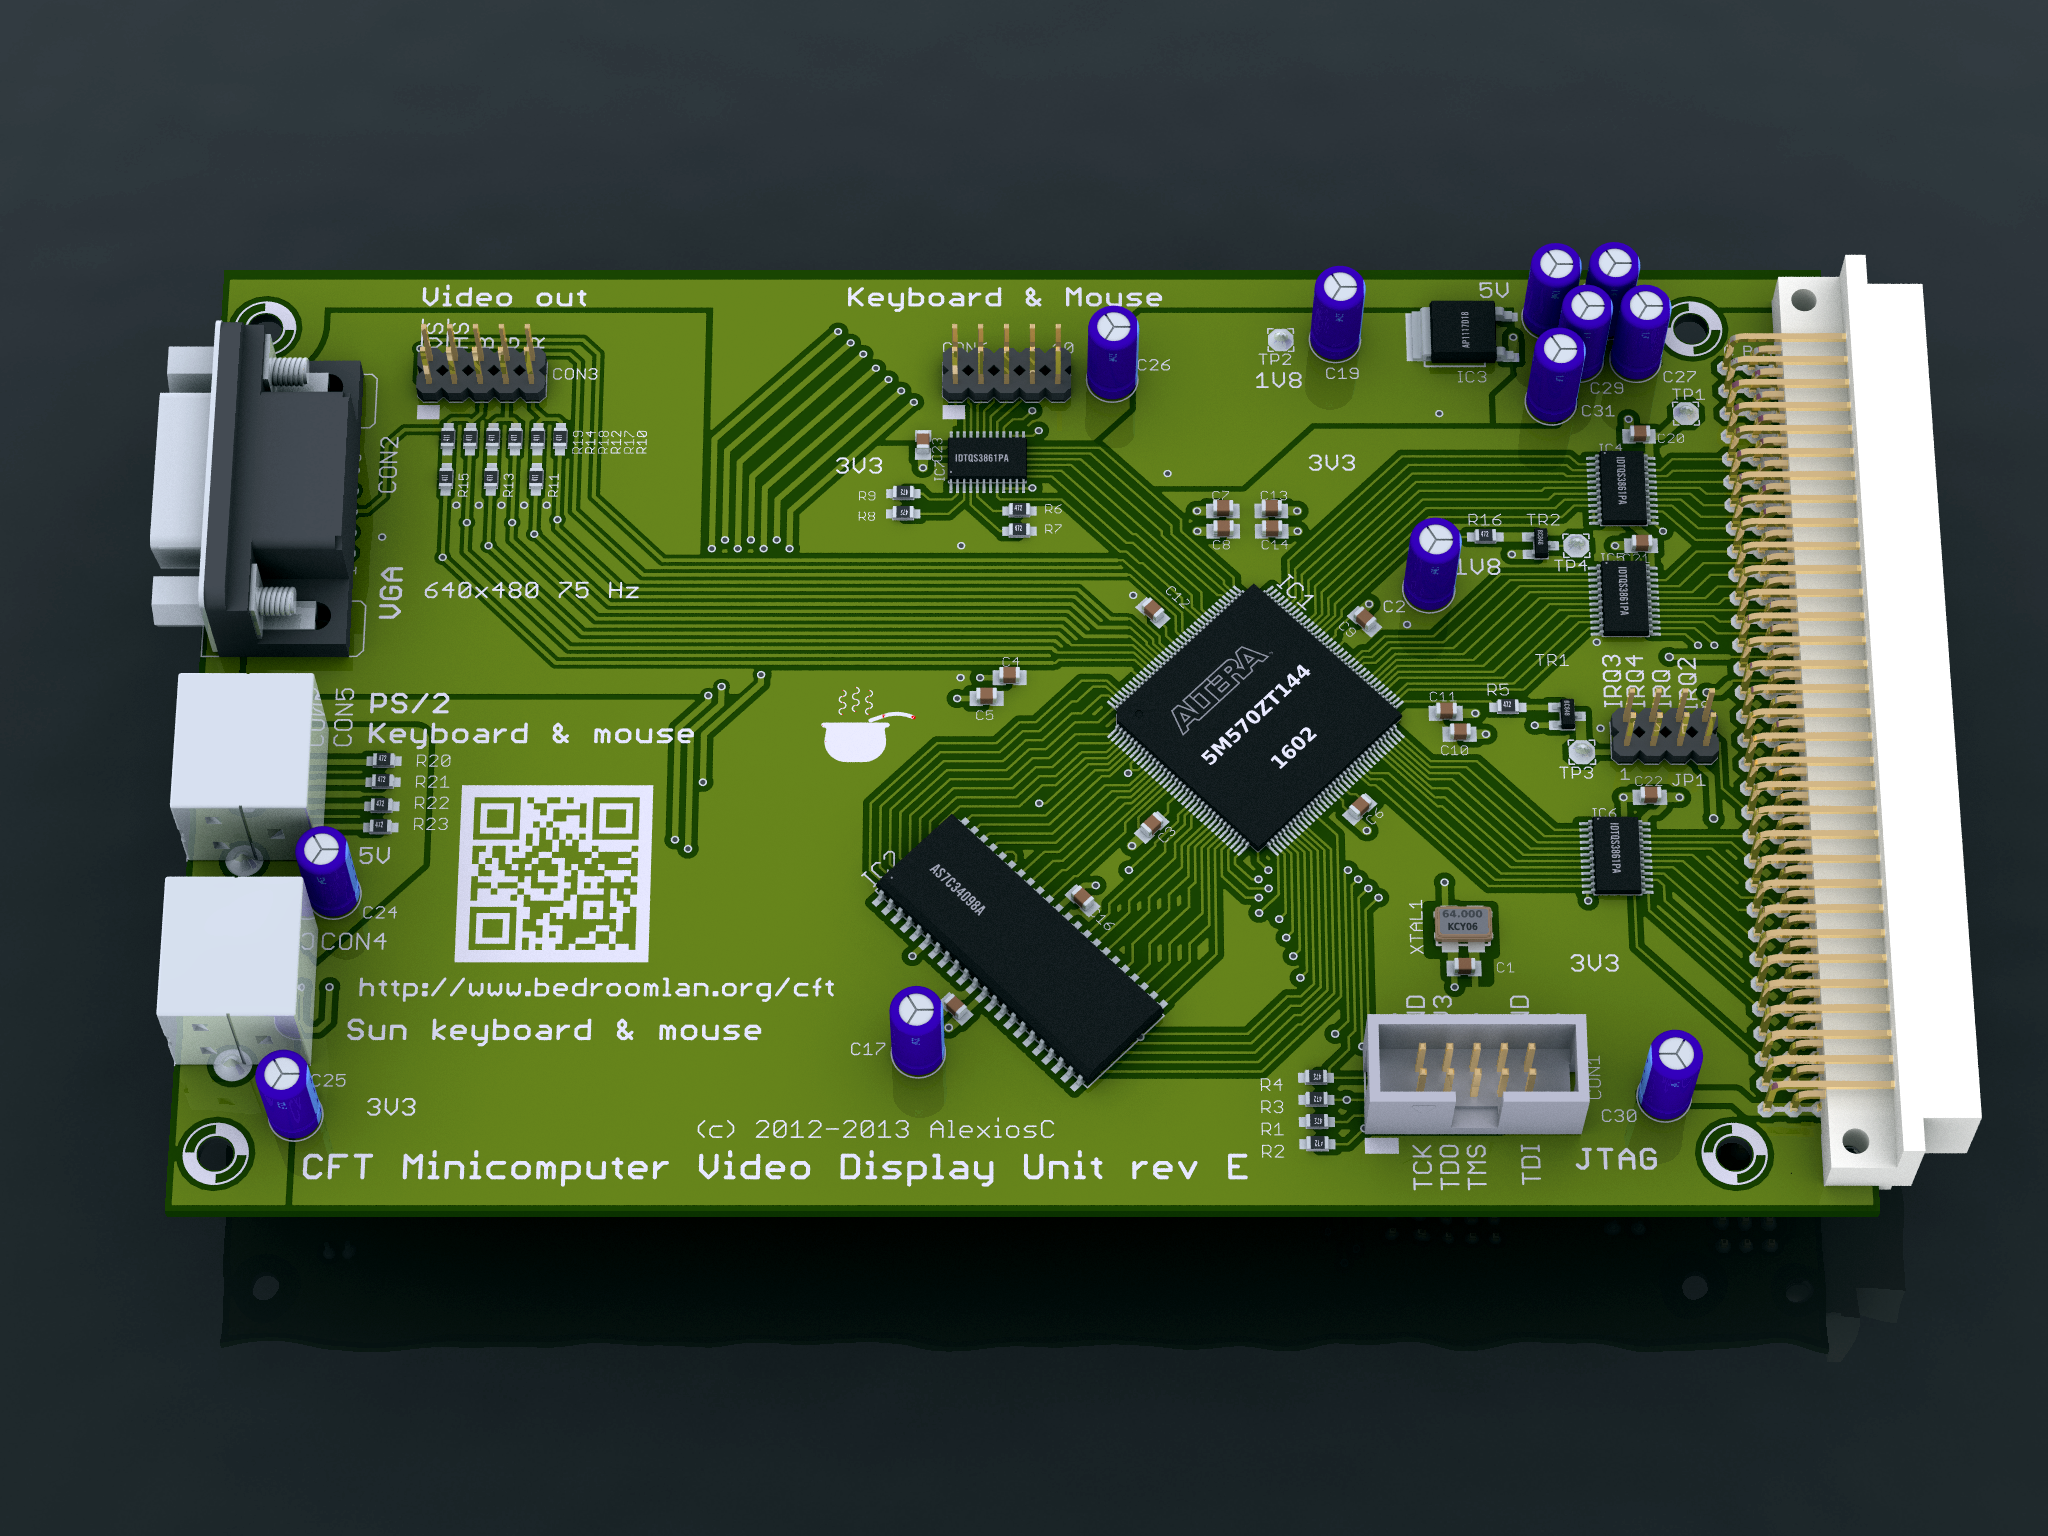
\includegraphics[width=0.85\columnwidth]{figs/cft-vdu-board3.png}\vspace{1em}\\
\caption{\label{fig:vdu-board}A rendered image of the VDU board. The CPLD makes
  the design quite sparse, and routing the board is easy — after all, the pins
  can be assigned any function and re-ordered at will to match the board
  layout.}
\end{figure}


\subsection{Video Format}

A video frame consists of a number of scan lines, each made of a
number of pixels, as shown in~\fcf{fig:video-frame-format}.

Each line is sent to the display serially, left to right. To help monitor
timing, lines start with a horizontal sync pulse (\ns{HSYNC}) to help
synchronise the framebuffer and display. This pulse is preceded by a number of
‘blank’ pixels known as the ‘front porch’, and followed by a similar zone
called the ‘back porch’. The horizontal sync pulse signals the display to begin
a new field. So, counter-intuitively, the front porch is the {\em end\/}
(right) of the previous field, and the back porch is the beginning of the
next. The formal horizontal waveform is shown in~\fcf{fig:vdu-horz-timing}.

Multiple fields are sent to the display serially, top to bottom. A blanked Front
Porch is sent first, followed by a vertical sync pulse (\ns{VSYNC}), followed
by a Back Porch and a number of fields in the format described above. Since
\ns{VSYNC} instructs the display to move to the top of the screen, starting a
new frame, the vertical Front Porch will appear at the bottom of the {\em
  previous\/} frame, while the Back Porch will appear at the top of the next
frame. The formal vertical waveform is shown in~\fcf{fig:vdu-vert-timing}.

The width of each of these subfields of each field and frame is expressed in
ticks of a {\em pixel clock\/}. A video format or mode is thus defined in terms
of the following nine parameters (often expressed in terms of other parameters,
arithmetically derived from these):

\begin{itemize}
\item The frequency or period of the pixel clock. This controls the physical size of each pixel on the screen, as well as the display resolution. It serves as the unit of timing, and all other parameters are expressed in terms of integer multiples of the pixel clock period.
\item The number of horizontal front porch pixels.
\item The number of horizontal video pixels. This is the same as the horizontal resolution in pixels.
\item The number of horizontal back porch pixels.
\item The number of pixels for which horizontal sync is active.
\item The number of vertical front porch pixels.
\item The number of vertical video pixels. This is the same as the vertical resolution in pixels.
\item The number of vertical back porch pixels.
\item The number of pixels for which vertical sync is active.
\end{itemize}

The CFT's VDU produces a single timing mode which produces an almost standard
VESA 640×480 resolution (at 74 frames per second, where VESA specifies 75)
using the following timings:

\begin{center}
\label{table:vdu-timings}
\zebra
\begin{tabular}{lrlrl}
            & Value & Unit & Time & Unit \\
\hline
Pixel clock frequency            &   32.000 & MHz    &  31.2500 & ns \\
\hline
Horizontal Front Porch width     &       24 & pixels &  0.7500 & μs \\
Horizontal Sync width            &       40 & pixels &  1.2500 & μs \\
Horizontal Back Porch width      &      128 & pixels &  4.0000 & μs \\
Horizontal Line width            &      640 & pixels & 20.0000 & μs \\
Total line width                 &      832 & pixels & 26.0000 & μs \\
Line (horizontal sync) frequency &   38.462 & kHz    & 26.0000 & μs \\
\hline
Vertical Front Porch height      &        9 & lines &   0.2340 & ms \\
Vertical Sync height             &        3 & lines &   0.0780 & ms \\
Vertical Back porch height       &       28 & lines &   0.7280 & ms \\
Vertical video height            &      480 & lines &  12.4800 & ms \\
Total frame height               &      520 & lines &  13.5200 & ms \\
Frame frequency (refresh rate)   &   73.965 & Hz    &  13.5200 & ms \\
\hline
\end{tabular}
\end{center}

These timings were generated using the VESA Co-ordinated Timing Generator
spreadsheet\footnote{Available at
  \url{http://files.bedroomlan.org/cft/video-board/CVTd6r1.xls}.} to maximise
compatibility and were tested on a number of monitors.

A horizontal resolution of 640 was chosen because it allows for 80 columns of
8-pixel wide characters. The vertical resolution of 480 was a more difficult
choice. 480 lines provide a classical 4:3 aspect ratio. Even though this is
running at a very slightly non-standard refresh rate, it is well within
tolerance for most, if not all multisync devices and works particularly well
with TFT monitors, producing images as crisp as can be expected from an
interpolated scaled up image.

A number of other resolutions were originally considered and ruled out:

\begin{itemize}
\item the 320×200 MCGA resolution is actually a 640×400 resolution with
  horizontal and vertical pixel doubling, implemented this way because the
  horizontal scan frequency of single-frequency VGA monitors was 31.15~kHz. As
  such, this would reduce the pixel resolution but still have the same timing
  requirements.
\item the 640×200 CGA resolution is, again, a 640×400 resolution with vertical
  line doubling and pixels with an aspect ratio of 8:3 — not particularly
  pleasing or useful. Since the horizontal resolution is the biggest hurdle in
  timing, this was also abandoned.
\item The 640×350 EGA-compatible resolution is a VGA 640×400 resolution with taller front
  and back porches, and the wrong pixel aspect ratio for modern monitors. Like
  the resolutions above, it made no sense to use it.
\item 640×400 was also attempted, and the design ran on this resolution for a
  while.  This is a 16:10 aspect ratio mode, so displays either slightly
  distorted on modern 16:9 devices, or using pillarboxes (narrow black bars at
  the left and right edge of the screen). This depends on the monitor
  used. However, many TFT monitors had trouble displaying a crisp image at this
  resolution. Additionally, the standard VGA pixel clock (25.175~MHz) for
  640×400 could not be used: the VDU design needed a clock double that of the
  pixel clock to allow both video and host accesses to the video memory, and
  there are no 50.35~MHz oscillators in the market.
\end{itemize}



\begin{figure}
 \centering     
 % -*- latex -*-
\documentclass[class=memoir,preview]{standalone}
% -*- latex -*-
\usepackage{pgf}
\usepackage{tikz}
%\usetikzlibrary{arrows,positioning,automata,shadows,fit,shapes,counters}
\usetikzlibrary{arrows,positioning,automata,shadows,fit,shapes,patterns}
%\usetikzlibrary{external}
%\tikzexternalize[prefix=tikz/]
%\tikzset{external/system call={xelatex \tikzexternalcheckshellescape -halt-on-error -interaction=batchmode -jobname "\image" "\texsource"}}
\usepackage{standalone}

\usepackage{layout}

%\usepackage[tocindentauto]{tocstyle}

%\usepackage[cam,a4,center]{crop}

\hypersetup{
    pdftitle={CFT Minicomputer Programming Guide},
    pdfauthor={Alexios Chouchoulas},
    pdfkeywords={},
    bookmarksnumbered,
    pagebackref=true,
    breaklinks=true,
%    pdfview=FitH,       % Or try pdfstartview={FitV}, This lead to uncorrect bookmarks
    urlcolor=darkblue,
    colorlinks=true,
    citecolor=cftoutline,          %citeref's color
    linkcolor=cftoutline,
        }

\makeindex
\makeglossaries
% -*- latex -*-

\renewcommand\glspostdescription{}

\newcommand\newglossaryabbr[3]{%
  \newglossaryentry{abbr#1}{name=\glslink{#1}{#2}, text={#2}, description={#3}}
  \newacronym[description={\glslink{abbr#1}{#2}}]{#1}{#1}{#2}
}

\newglossaryentry{IBUS}{name=IBUS,
  description={
  Internal Bus: the single, internal 16-bit bus of the CFT processor.
  }}
  
\newglossaryentry{Data Bus}{name=Data Bus, description={ A
    16-bit bus used to move data between the processor and
    peripherals.  }}
  
\newglossaryentry{Address Bus}{name=Address Bus, description={A
    16-bit bus used to select a peripheral nor memory location to
    access.}}
  
\newglossaryentry{Video Display Unit}{name=Video Display Unit,
  description={ Video Display Unit (VDU): a device that drives a
    display monitor to show character or graphics data on a
    screen. Often also contains one or more input devices (keyboard,
    mouse).}}
  
\newglossaryentry{von Neumann architecture}{name=Von Neumann architecture,
  description={ Named after the work of
    John von Neumann, the von Neumann architecture is a ‘modern’
    computer architecture that includes a register file, arithmetic
    and logic units, memory and input/output, and uses the same
    storage for programs and data.}}

\newglossaryentry{stored program computer}{name=Stored program computer,
  description={ A type of computer that
    uses the same storage for programs and data. All modern computers
    are stored program computers, allowing self-modification of their
    programs. Early designs and many modern microcontrollers stored
    programs and data in separate media, and did not or could not
    treat programs as data.}}

\newglossaryabbr{ALU}{Arithmetic/Logic Unit}{Describe this!}
\newglossaryabbr{ISR}{Interrupt Service Routine}{Describe this!}
\newglossaryentry{UART}{name=UART, description={
    Short for Universal Asynchronous Receiver/Transmitter. UARTs are
    devices that handle asynchronous serial communications such as RS-232, RS-485 or USB.
    }
}
%% \newglossaryentry{alu}{name=\glslink{ALU}{Arithmetic/Logic Unit}, text=Arithmetic/Logic Unit,
%%   description={TODO}}
%% \newacronym[description={\glslink{alu}{Arithmetic/Logic Unit}}]{ALU}{ALU}{Arithmetic/Logic Unit}

\newacronym{SBU}{SBU}{Skip/Branch Unit}

\newacronym{AGL}{AGL}{Address Generation Logic}

\newglossaryentry{DEB}{name=DEB, description={
    Designation of the CFT Debugging/Testing board, a peripheral that
    allows remote control and testing of the computer and its
    peripherals in the style of a virtual front panel. The DEB board
    is discussed in~\ccf{chap:deb}.
}}

\newglossaryentry{VDU}{name=VDU, description={ Video Display
    Unit. Designation of the CFT graphic card and keyboard
    controller. The VDU board is discussed in~\ccf{chap:vdu}.  }}

\newglossaryentry{MSB}{name=MSB, description={
    Most Significant Bits. Usually used to refer to the upper eight bits of a CFT word.
}}
\newglossaryentry{LSB}{name=LSB, description={
    Least Significant Bits. Usually used to refer to the lower eight bits of a CFT word.
}}

\newglossaryentry{NYBBLE}{name=Nybble, description={Sometimes
    nibble. A four-bit quantity, represented as a single hexadecimal
    digit.
}}

% \newacronym{MCU}{MCU}{Micro-Controller Unit}

\newglossaryabbr{MCU}{Micro-Controller Unit}{A single-chip device
  containing a simple microprocessor, general purpose input/output,
  serial input/output, timers, and other useful devices.}

\newacronym{USB}{USB}{Universal Serial Bus}

\newacronym{GPIO}{GPIO}{General-Purpose Input/Output}

\newglossaryentry{Verilog}{name=Verilog,
  description={
    One of the two major hardware
    description languages, the other being VHDL. In the CFT project,
    Verilog is used to perform 74xxx chip-level simulation and
    verification of the CFT processor.
}}

\newglossaryentry{I2C}{name=I²C, description={A two-wire, open-drain
    bus, often used for communication between \gls{MCU}s and
    peripheral chips, including EEPROMs and sensors. For more
    information, please consult
    \url{http://en.wikipedia.org/wiki/I2C}.}}

\newglossaryentry{data stack}{name=Data Stack,
  description=To Do}

\newglossaryentry{postfix}{name=postfix,
  description=To Do}

\newglossaryentry{stack effect comment}{name=stack effect comment,
  description=To Do}

\newglossaryentry{Wait State}{name=Wait State, 
  description={An additional state added to the processor state machine
  to accommodate slow devices. External devices signal their need for a
  wait state to the processor using an appropriate procotol. The
  processor then enters the Wait State and does not leave until the
  device is ready. The processor performs no action during this time,
  hence the name.}}


\newglossaryentry{Twos Complement}{name=Two's Complement,
  description={Currently the most popular means of representing signed
    integers in binary. For a bit width $n$, non-negative numbers $0 \leq
    x < 2^{n-1}$ are represented as unsigned $n$-bit binary
    integers. Negative numbers $-2^{n-1} \leq x < 0$ are represented in
    the form $2^n - x$, with the most significant bit set. On the CFT,
    with $n=16$, this provides a signed range of $[-32,768,
      32,767]$. Two's complement has many useful mathematical
    properties: only one representation of zero, the most significant
    bit also acts as a sign bit, and both addition and subtraction can
    be performed by the same circuitry. For a full discussion, please refer
    to \url{http://en.wikipedia.org/wiki/Two's\_complement}.  }}

\newglossaryentry{Assembly}{name=Assembly, description={A symbolic form of
    \gls{machine code}, meant to be used by humans. Some architectures,
    including the CFT, have simple machine code that can be learned in minutes,
    but the human brain deals better with symbols. Assembly languages also
    provide productivity enhancing features like comments, labels, macros,
    simple arithmetic for literals, and other such facilities. The CFT
    Assembler provides all of these facilities.  }}

\newglossaryentry{DIP}{name=DIP, description={Dual In-line Package, the
    most common integrated circuit package until the introduction of
    Surface Mount Technology: DIP chips have two rows of pins, with pins
    set at distances of 2.54~mm (0.1~inch).
}}

\newglossaryentry{PLCC}{name=PLCC, description={Plastic Leaded Chip
    Carrier, a square surface mount chip packaging easily adapted to
    2.54mm grids by means of suitable IC sockets. The CFT uses
    numerous PLCC chips to save board space and because they offer
    more choice of chips, and thus better value for money. All CFT
    PLCC packages are either Flash devices or UARTs.}}

\newglossaryentry{MEM}{name=MEM, description={ Designation of the
    memory board, which, depending on construction details provides up
    to 512 or 1,024 kWords of RAM and/or ROM. The MEM board is
    discussed in~\ccf{chap:mem}.
}}

\newglossaryentry{MBU}{name=MBU, description={Designation of the
    Memory Banking Unit. This was originally slated to be a separate
    peripheral, but has become so important to the project that it is
    now considered to be part of the processor, and constructed as
    such. The MBU breaks memory space in logical and physical
    addresses, and allows the processor's limited 64 kWord address
    space to be expanded to a 21 bit, 2,048 kWord address space using
    memory banking techniques. More details may be found in
    \ccf{chap:mbu}.  }}

\newglossaryentry{Interrupt Service Routine}{name=Interrupt Service Routine (ISR),
  description={TO DO}}

\newglossaryentry{Page}{name=Page, description={The CFT instruction set allows
    for a 10-bit operand, which allows instructions to address up to
    $2^{10}=1024$ locations. This 1,024-word range is known as a page. The CFT
    address space contains 64 such 1 kWord pages. \gls{Page Zero} at addresses
    \hex{0000}–\hex{03FF} has special significance in the programming model, as
    discussed in~\cf{sec:memory-space}.
 }}

\newglossaryentry{Page Zero}{name=Page Zero, description={Page Zero occupies
    the first 1,024 addresses (\hex{0000}–\hex{03FFF}) of the memory address
    space. It is used to simulate 1,024 registers, global variables or
    constants accessible from anywhere in memory. Addresses
    \hex{0080}–\hex{00FF} are autoindex locations: they increment when accessed
    in \gls{Indirect Mode}.}}

\newglossaryentry{Addressing Mode}{name=Addressing Mode, description={An
    addressing mode is the method in which an instruction operand is
    interpreted. The CFT can treat operands as literal values (\gls{Literal
      Mode}), addresses of data (\gls{Direct Mode}), or addresses of addresses
    of data (\gls{Indirect Mode}), similar to pointersin high-level languages
    such as C and Pascal. Addressing modes are discussed
    in~\cf{sec:addressing-modes}}.}

\newglossaryentry{Indirect Mode}{name=Indirect Mode, description={An addressing
    mode where an instruction operand identifies the memory location which
    contains the address of the data to access. Compare \gls{Direct
      Mode}. Addressing modes are discussed in~\cf{sec:addressing-modes}.}}

\newglossaryentry{Direct Mode}{name=Direct Mode, description={An addressing
    mode where an instruction operand identifies the memory location of the
    data to access. Compare \gls{Indirect Mode}. Addressing modes are discussed
    in~\cf{sec:addressing-modes}.}}

\newglossaryentry{Literal Mode}{name=Literal Mode, description={An addressing
    mode where an instruction operand identifies the memory location of the
    data to access. Compare \gls{Indirect Mode}. Addressing modes are discussed
    in~\cf{sec:addressing-modes}.}}

\newglossaryentry{register}{name=Register, description={ A data storage device
    inside a processor. Registers are usually faster than memory, and so are
    used to store intermediate results. In many architectures, notably
    \glspl{ABA}, the only way for the processor to
    manipulate data is to transfer it to a register, operate on the register,
    then transfer it back to its intended location. CFT registers are discussed
    in~\cf{sec:registers}.}}

\newglossaryentry{Accumulator}{name=Accumulator, description={The main
    \gls{register} in an \gls{ABA}. Data must be transferred to the Accumulator
    before it can be operated on by the processor. In the CFT, the Accumulator
    is the only such general purpose register available. The term comes from
    the days of tabulating machines, which used accumulators to accumulate
    (sum) numbers. The Accumulator is designated ‘\AC’ on the CFT. Its hardware
    design is discussed in~\cf{sec:major-registers} and its operation from a
    programmer's point of view is discussed in~\cf{sec:accumulator}.}}

\newglossaryabbr{ABA}{Accumulator-Based Architecture}{A processor architecture
  built around a single (or in some cases, a few) accumulators. Most early
  computers followed this design because of its simplicity, and the CFT does
  too. Having a single register draastically simplifies the instruction format,
  too: from a two-operand instruction format (source, destination), we move to
  a single operand (source or destination). The other operand is always the
  accumulator.  }

\newglossaryentry{nybble}{name=Nybble, description={(sometimes nibble)
    A 4-bit quantity, corresponding to one hexadecimal digit, half a
    byte, or one quarter of a CFT \gls{Word}.}}

\newglossaryentry{Word}{name=Word, description={One CFT Word is a
    16-bit quantity. CFT memory and I/O accesses transfer exactly one
    word each. CFT instructions are also one Word wide. This is not to
    be confused with the Forth concept of a \gls{word} (an identifier).}}

\newglossaryentry{word}{name=Word, description={A Forth word is any
    sequence of non-whitespace characters that is not a number. This
    is not to be confused with the more common concept of the
    \gls{Word} as a numeric datatype.}}

\newglossaryentry{machine code}{name=Machine code, description={Machine code is
    the native language of every processor, where machine instructions and data
    are represented in binary. Machine code is easy for the computer to
    process, but humans find it useful to apply abstraction layers to it: data
    are represented in other bases (octal, decimal and hexadecimal being the
    most common), and symbolic instruction names (rather than binary
    instruction numbers) are used. This set of abstractions is \gls{Assembly}
    language.}}

\newglossaryentry{disk label}{name=Disk Label, description={ A disk label
    stores information about a storage device (not always a disk), including a
    magic number to help detect the block, some optional boot code, and
    definitions for one to sixteen \glspl{disk slice} (partitions). The disk
    label always resides in the first block of a device. The best-known disk
    label format is the MS-DOS Master Boot Record, MBR. The CFT's disk label is
    discussed in~\cf{sec:disk-label}.}}

\newglossaryentry{disk slice}{name=Disk Slice, description={Part of a disk intended to
    hold a \gls{filesystem} or other data. Disks are sliced to make them easier
    to manage, so different operating systems can be used, to control the size
    of stored data, and to avoid corruption in one filesystem destroying all
    data. In the MS-DOS world, slices are known as ‘partitions’, and the
    \gls{disk label} is known as a ‘partition table’ or ‘Master Boot Record’
    depending whether it resides on a data disk or bootable disk. The CFT's
    slice scheme is discussed in~\cf{sec:disk-slices}}.}

\newglossaryentry{filesystem}{name=Filesystem, description={ A large data
    structure used to view a storage medium as a hierarchical collection of
    data objects called files. The filesystem abstracts the natural
    array-of-blocks structure of the storage medium, and provides the user with
    an interface for creating, reading and otherwise operating on files by
    their name, location and other attributes. Files can be larger than the
    natural block size, and this is again handled transparently by the
    filesystem code. The CFT's filesystem is described in~\cf{sec:fs}}}

\newglossaryabbr{VD}{Volume Directory}{A data structure
  describing a CFT \gls{filesystem}. Comparable to a Unix filesystem
  superblock. The VDD is the exact same data structure as a
  \gls{DD}. The difference is in the magic number and the contents of
  the first directory slot (the header), which contains a volume
  header structure.}

\newglossaryabbr{DD}{Directory Descriptor}{A data structure describing
  a directory in a CFT \gls{filesystem}.}

\newglossaryentry{block pointer}{name=Block Pointer, description={A
    32-bit value (\gls{MSB} first) denoting the number of a filesystem
    block. A filesystem's first block is block \hex{00000000}.}}

\newglossaryabbr{DH}{Directory Header}{A data structure describing a
  CFT directory. This is the first entry of a \gls{DD}.}

\newglossaryabbr{OOP}{Object Oriented Programming}{A programming
  paradigm where data and code are bundled together in data structures
  called objects. Programs are built based on the interactions and
  interrelations of these objects.}

\newglossaryentry{descriptor}{name=Descriptor, description={In the CFT Filesystem, a data structure
    that holds metadata on an object in the CFT filesystem. Descriptors share
    some common metadata (e.g. filenames, flags, creation time and date). They
    are located inside container objects (volumes and directories). Containers
    and descriptors are discussed in~\cfp{sec:fs-containers}.}}

\newglossaryentry{volume}{name=Volume, description={A \gls{disk slice} which
    has been structured according to the CFT Filesystem. In \gls{OOP} terms, a
    volume is the object (instance) and the CFT Filesystem is the class.}}

\newglossaryentry{container}{name=Container, description={In the CFT
    Filesystem, a data structure that contains other filesystem objects. Entire
    filesystem \glspl{volume} are containers, and so are directories. Each
    container owns a maximum number of \glspl{descriptor}, identifying the
    contained objects. Once this limit is reached, continuation blocks are
    allocated for the container. These continuation blocks form a doubly linked
    list. Containers are discussed in~\fcf{sec:fs-containers}.}}

\newglossaryabbr{PEL}{Picture Element}{The smallest addressable
  picture element of a display mode. A PEL is usually a block of
  multiple pixels.}

\newglossaryabbr{MTBF}{Mean Time Between Failures}{The average life
  expectancy of a device.}

\newglossaryentry{codepoint}{name=Codepoint, description={A number
    identifying a character within a character set. For example, in
    the ASCII set, codepoint 65 is the character ‘A’.}}

\newglossaryabbr{SDRAM}{Synchronous Dynamic Random Access Memory}{A
  type of modern dynamic RAM that operates using a clock, not
  asynchronously like original DRAMs. The memory contains a command
  pipeline, because data appears on the bus two to three clock ticks
  after a read is signalled. Multiple reads are pipelined, making the
  memory very fast for many use patterns.}

\newglossaryabbr{SRAM}{Static Random Access Memory}{A type of
  relatively low-density memory that trades off capacity and price for
  speed and interface simplicity. SRAMs do not need to be refreshed
  and are faster than similar dynamic RAMs.}

\newglossaryentry{extended instruction}{name=Instruction!Extended,
  description={An address in I/O space that provides side effects
    useful enough to be seen as extending the processor's instruction
    set. They are usually aliases of single \asm{IN}, \asm{OUT} or
    \asm{IOT} instructions.}}

\newglossaryabbr{SR}{Switch Register}{A 16-bit read-only register that
  provides the value of the 16 data entry switches on the front
  panel.}

\newglossaryabbr{DSR}{DIP Switch Register}{A 12 to 16-bit read-only
  register driven by a bank of DIP switches on the Front Panel
  Controller board. The DSR can be used to set non-volatile prefrences
  for the computer's early boot.}

\newglossaryabbr{MFD}{Multi-Function Display}{A bank of 16 lights on
  the front panel which can display a user-selectable register. The
  user can elect to show the value of the Data Register, Output
  Register, or the 15-bit microcode store address. A switch on the
  front panel is used to do this.}


\usepackage{listings}
\lstset{%
  xleftmargin=35pt,
  xrightmargin=5pt,
  basicstyle={\ttfamily},
  backgroundcolor=\color{cfthl!25},
  rulecolor=\color{cfthl!25},
  framesep=5pt,
  rulesep=5pt,
  frame=tlrb,
  framexleftmargin=10pt,
  flexiblecolumns=true,
  keepspaces=true,
  numbers=left,
  numbersep=5pt,
  numberstyle={\scriptsize\sffamily\color{cftlight}}
}




%%%%%%%%%%%%%%%%%%%%%%%%%%%%%%%%%%%%%%%%%%%%%%%%%%%%%%%%%%%%%%%%%%%%%%%%%%%%%%%
%%
%% LISTS OF THINGS
%%
%%%%%%%%%%%%%%%%%%%%%%%%%%%%%%%%%%%%%%%%%%%%%%%%%%%%%%%%%%%%%%%%%%%%%%%%%%%%%%%

%% %%%\addtolength\cftfignumwidth{1.5em}
\makeatletter
%% \addtolength{\cftchapternumwidth}{0.5em}
%% \addtolength{\cftsectionnumwidth}{0.5em}
%% \addtolength{\cftsubsectionnumwidth}{0.5em}
%% \addtolength{\cftfigurenumwidth}{0.5em}
%% \addtolength{\cfttablenumwidth}{0.5em}
\renewcommand*\l@section{\@dottedtocline{1}{1.5em}{2.3em}}
\renewcommand*\l@subsection{\@dottedtocline{2}{3.8em}{3.2em}}
\renewcommand*\l@subsubsection{\@dottedtocline{3}{7.0em}{4.1em}}
\renewcommand*\l@paragraph{\@dottedtocline{4}{10em}{5em}}
\renewcommand*\l@subparagraph{\@dottedtocline{5}{12em}{6em}}
\setcounter{maxsecnumdepth}{3}

%\addtolength{\cftschematicsnumwidth}{1em}
\renewcommand{\@pnumwidth}{3em}
\renewcommand{\@tocrmarg}{4em}
\makeatother

%\newcommand\listalgname{List of Algorithms} 
%\newlistof{alg}{algorithm}

%
% Schematics
%

\newcommand\listschematicname{List of Schematics} 
\newlistof{listofschematic}{los}{\listschematicname}
\newcounter{schematic}
\newcommand{\schematic}[1]{%
  \refstepcounter{schematic}%
  \par\noindent\textbf{Schematic \theschematic. #1}
  \addcontentsline{los}{section}{\protect\numberline{\theschematic}#1}\par%
}
\newcommand\listofschematics\listofschematic

%
% I/O Ports
%

\newcommand\listioportname{List of Input/Output Ports} 
\newlistof{listofioport}{loioport}{\listioportname}
%% \newcommand{\registerioport}[1]{%
%%   \refstepcounter{ioport}%
%%   \addcontentsline{loioport}{section}{\protect\numberline{\ }%
%% }
\newcommand\listofioports\listofioport



\newcommand\caution[1]{\textcolor{caution}{\textbf{#1}}}
%\newcommand\todo[1]{\textcolor{caution}{\bf{TODO: #1}}}

%
% Tasks
%

\newcommand\listtasksname{List of Incomplete Tasks} 
\newlistof{listoftask}{lotasks}{\listtasksname}
\newcounter{task}
\newcommand{\todo}[1]{%
  \refstepcounter{task}%
  {\textcolor{caution}{\textbf{TODO: #1}}}
  \addcontentsline{lotasks}{section}{\protect\numberline{\arabic{task}}To Do: #1}\par%
}
\newcommand{\bug}[2]{%
  \refstepcounter{task}%
  {\textcolor{caution}{\textbf{BUG: #1 #2}}}
  \addcontentsline{lotasks}{section}{\protect\numberline{\arabic{task}}Bug: #1}\par%
}
\newcommand\listoftasks\listoftask

%
% Data structures
%

\newcommand\listdatastructurename{List of Data Structures} 
\newlistof{listofdatastructure}{lods}{\listdatastructurename}
\newcounter{datastructure}
%\newcommand{\datastructure}[1]{%
%  \refstepcounter{datastructure}%
%  \par\noindent\textbf{Data Structure \thedatastructure. #1}
%  \addcontentsline{lods}{section}{\protect\numberline{\thedatastructure}#1}\par%
%}
\newcommand\listofdatastructures\listofdatastructure



%%%%%%%%%%%%%%%%%%%%%%%%%%%%%%%%%%%%%%%%%%%%%%%%%%%%%%%%%%%%%%%%%%%%%%%%%%%%%%%
%%
%% SECTION STYLING
%%
%%%%%%%%%%%%%%%%%%%%%%%%%%%%%%%%%%%%%%%%%%%%%%%%%%%%%%%%%%%%%%%%%%%%%%%%%%%%%%%



%% \usepackage{kpfonts}
\usepackage[explicit]{titlesec}

\counterwithin*{chapter}{part}
\counterwithin*{figure}{chapter}
\counterwithin*{schematic}{chapter}
\counterwithin*{datastructure}{chapter}
\counterwithin*{table}{chapter}

%%%%%%%%%%%%%%%%%%%%%%%%%%%%%%%%%%%%%%%%%%%%%%%%%%%%%%%%%%%%%%%%%%%%%%%%%%%%%%%

\renewcommand\thepart{\Alph{part}}
\cftpagenumbersoff{part}
%\newcommand*\partlabel{}

\makeatletter
\patchcmd{\l@part}{\hss#2}{}{}{}
\makeatother


\renewcommand\partnamefont{\normalfont\sffamily\Huge\scshape}
\renewcommand\partnumfont{\bfseries}
\renewcommand\printparttitle[1]{
  \thispagestyle{empty}
    \begin{tikzpicture}[remember picture,overlay]
      \node[yshift=-\paperheight, draw opacity=0] at (current page.north west)
           {\begin{tikzpicture}[remember picture, overlay]
               \draw[fill=cftlight] (0,0) rectangle
               (\paperwidth,\paperheight);
               \draw[fill=cftoutline] (0,1cm) rectangle
               (\paperwidth,0);
               \node[anchor=east,yshift=0.5\paperheight,xshift=.87\paperwidth,rectangle]
                    {\scalebox{2}{\color{white}\printpartname~\printpartnum}};
                    \node[anchor=east,yshift=0.43\paperheight,xshift=.87\paperwidth,rectangle]
                         {\scalebox{1.5}{\color{white} #1}};
             \end{tikzpicture}
           };
    \end{tikzpicture}
}


\newcommand*\chapterlabel{}
\titleformat{\chapter}
  {\gdef\chapterlabel{}
   \normalfont\sffamily\Huge}
  {\gdef\chapterlabel{\thechapter\ }}{0pt}
  {%
    \setcounter{page}{1}
    \begin{tikzpicture}[remember picture,overlay]
    \node[yshift=-5cm, draw opacity=0] at (current page.north west)
      {\begin{tikzpicture}[remember picture, overlay]
        \draw[fill=cftlight] (0,0) rectangle
          (\paperwidth,5cm);
        \draw[fill=cftoutline] (0,0.25cm) rectangle
          (\paperwidth,0);
        \node[anchor=east,yshift=2cm,xshift=.87\paperwidth,rectangle]
              {\color{white}\chapterlabel#1};
       \end{tikzpicture}
      };
   \end{tikzpicture}
  }
\titlespacing*{\chapter}{0pt}{50pt}{20pt}

\titleformat{\section}
            {\gdef\sectionlabel{}\normalfont\sffamily\Large}
            {\gdef\sectionlabel{\thesection\ }}{0pt}
            {\color{cftoutline}\thesection\quad #1\\
              \titlerule[2pt]
            }[{\vspace{-30pt}\color{cftoutline}\rule{\textwidth}{2pt}}]


\titleformat{\subsection}
  {\gdef\subsectionlabel{}
   \normalfont\sffamily\bfseries\large}
  {\gdef\subsectionlabel{\thesubsection\ }}{0pt}
  {\color{cftoutline}\thesubsection\quad #1}


\titleformat{\subsubsection}
  {\gdef\subsubsectionlabel{}
   \normalfont\sffamily\large}
  {\gdef\subsubsectionlabel{\thesubsubsection\ }}{0pt}
  {\color{cftoutline}#1}


%%%%%%%%%%%%%%%%%%%%%%%%%%%%%%%%%%%%%%%%%%%%%%%%%%%%%%%%%%%%%%%%%%%%%%%%%%%%%%%










%% \titleformat{\paragraph}
%%   {\gdef\chapterlabel{}
%%    \normalfont\bfseries}
%%   {\gdef\chapterlabel{\theparagraph\ }}{0pt}
%%   {\color{cftoutline}#1}



%\geometry{a4paper, hoffset=0in, voffset=-.25in, left=1.5cm, right=1.5cm,
%  top=2.5cm, bottom=2.5cm}
%\geometry{paperwidth=17.5cm, paperheight=23.1cm, hoffset=0in, voffset=-.25in, left=1in, right=1in,
%  top=1in, bottom=1in}
\geometry{a4paper, hoffset=0in, left=1.2in, right=1.2in,
  top=1.2in, bottom=1.2in, includefoot, footskip=40pt}
%\sloppy


% Fonts
%\defaultfontfeatures{Mapping=tex-text}
\setmainfont{Minion Pro}
\setsansfont{Myriad Pro}
\setmonofont[]{Inconsolata}


% Not really used here, but never mind.
\setlength\columnsep{7mm}


% Input our local macro definitions
% -*- latex -*-

\definecolor{caution}{RGB}{192,0,0}

\newcommand\textcond{\fontspec{Myriad Pro Condensed}}

% Primary index entries
\newcommand\pie[1]{\textbf{\hyperpage{#1}}}

% Use hyperlinking when rendering PDFs
\newcommand{\barecf}[1]{\hyperref[#1]{\ref*{#1}}}
\newcommand{\cf}[2][section]{\hyperref[#2]{%
        \ifthenelse{\equal{\pageref*{#2}}{\thepage}}%
        {#1 \ref*{#2}}%
        {#1 \ref*{#2} (p.~\pageref*{#2})}%
}}
\newcommand{\cfp}[2][section]{\hyperref[#2]{%
        \ifthenelse{\equal{\pageref*{#2}}{\thepage}}%
        {#1 \ref*{#2}}%
        {#1 \ref*{#2}, p.~\pageref*{#2}}%
}}
\newcommand{\fcf}[1]{\cf[figure]{#1}}
\newcommand{\fcfp}[1]{\cfp[figure]{#1}}
\newcommand{\tcf}[1]{\cf[table]{#1}}
\newcommand{\tcfp}[1]{\cfp[table]{#1}}
\newcommand{\ccf}[1]{\cf[chapter]{#1}}
\newcommand{\ccfp}[1]{\cfp[chapter]{#1}}
%
\newcommand{\npcf}[2][section]{\hyperref[#2]{#1 \ref*{#2}}}
\newcommand{\appcf}[1]{\cf[appendix]{#1}}
\newcommand{\ecf}[1]{\cf[equation]{#1}}
\newcommand{\algcf}[1]{\cf[algorithm]{#1}}
\newcommand{\npappcf}[1]{\npcf[appendix]{#1}}
\newcommand{\npccf}[1]{\npcf[chapter]{#1}}
\newcommand{\npfcf}[1]{\npcf[figure]{#1}}
\newcommand{\nptcf}[1]{\npcf[table]{#1}}
\newcommand{\npecf}[1]{\npcf[equation]{#1}}
\newcommand{\npalgcf}[1]{\npcf[algorithm]{#1}}

\newcommand\hyperemail[1]{\sffamily\href{mailto:#1}{#1}}
\newcommand\link[1]{\sffamily\href{http://#1}{#1}}
\newcommand\ahref[2]{\sffamily\href{#1}{#2}}

\newcommand\op[1]{{\ttfamily #1}}
\newcommand\fwni[1]{{\ttfamily{#1}}}
\newcommand\fw[1]{\fwni{#1}\index{#1@\protect\fwni{#1}}}
%                           \index{#1@\fwni{#1}|(pie}%

\newcommand\f[1]{{\texttt{#1}}}
\newcommand\hex[1]{\textsf{#1}}
\newcommand\bin[1]{\textsf{#1}}
\newcommand\bitmap[1]{\texttt{#1}}
\newcommand\bus[1]{{#1}}
\newcommand\unit[1]{{#1}}
\newcommand\IBUS{\bus{\gls{IBUS}\index{IBUS}}}
\newcommand\DBUS{\bus{\gls{Data Bus}\index{Data Bus}}}
\newcommand\ABUS{\bus{\gls{Address Bus}\index{Address Bus}}}
\newcommand\ALU{\unit{\gls{ALU}\index{ALU}}}
\newcommand\SBU{\unit{\gls{SBU}\index{SBU}}}
\newcommand\AGL{\unit{\gls{AGL}\index{AGL}}}
\newcommand\register[1]{\textsf{#1}\index{Registers!#1}}
\newcommand\A{\register{AC}}
\newcommand\AC{\A}
\newcommand\Areg{\A}
\newcommand\Lreg{\register{L}}
\newcommand\Ireg{\register{I}}
\newcommand\Zreg{\register{Z}}
\newcommand\Vreg{\register{V}}
\newcommand\Nreg{\register{N}}
\newcommand\AR{\register{AR}}
\newcommand\MAR{\AR}
\newcommand\DR{\register{DR}}
\newcommand\PC{\register{PC}}
\newcommand\IR{\register{IR}}

\newcommand{\asm}[1]{\texttt{#1}}
\newcommand{\instr}[1]{\asm{#1}}
\newcommand{\nsni}[1]{$\overline{\mbox{\textsf{{#1}}}}$}
\newcommand{\ns}[1]{\nsni{#1}\index{#1@{$\protect\overline{\protect\mbox{\textsf{#1}}}$}}}
\newcommand{\psni}[1]{\textsf{#1}}
\newcommand{\ps}[1]{\psni{#1}\index{#1@\psni{#1}}}
\newcommand{\lt}[1]{\textsf{#1}}
\newcommand{\sw}[1]{\textsf{#1\index{Switch, front panel!#1}}}
\newcommand{\HC}[1]{\chip{74HC{#1}}}
\newcommand{\HCT}[1]{\chip{74HCT{#1}}}
\newcommand{\chip}[1]{#1\index{#1}}

\newcommand{\schpt}[1]{#1\textsf{#1}}
\newcommand{\farnell}[1]{#1}

\newcommand\BUS[2]{\ps{#1}$_{\mbox{\scriptsize #2}}$}
\newcommand\nBUS[2]{\ns{#1}$_{\mbox{\scriptsize #2}}$}

\newcommand\UINSTR{\ns{uINSTR18}}
\newcommand\HALT{\ns{HALT}}
\newcommand\END{\ns{END}}
\newcommand\IRQ{\ns{IRQ}}
\newcommand\IRQS{\ns{IRQS}}
\newcommand\IRQn[1]{\nBUS{IRQ}{#1}}
\newcommand\RUNITn[1]{\BUS{RUNIT}{#1}}
\newcommand\WUNITn[1]{\BUS{WUNIT}{#1}}
\newcommand\TPA{\ps{TPA}}
\newcommand\TPC{\ps{TPC}}
\newcommand\WAC{\ns{WAC}}
\newcommand\WALU{\ns{WALU}}
\newcommand\WDR{\ns{WDR}}
\newcommand\WIR{\ns{WIR}}
\newcommand\WMAR{\ns{WMAR}}
\newcommand\WPC{\ns{WPC}}
\newcommand\SYSDEV{\ns{SYSDEV}}
\newcommand\IODEV[1]{\ns{IODEV{#1}XX}}
\newcommand\OPIFn[1]{\BUS{OPIF}{#1}}
\newcommand\OPIF{\ps{OPIF}}
\newcommand\GUARDPULSE{\ns{GUARD}}
\newcommand\GP{\GUARDPULSE}
\newcommand\CLOCK[1]{\BUS{CLK}{#1}}
\newcommand\RSTHOLD{\ns{RSTHOLD}}
\newcommand\BOE{\ns{BOE}}
\newcommand\UOE{\ns{UOE}}
\newcommand\SKIP{\ns{SKIP}}
\newcommand\AINDEX{\ps{AINDEX}}
\newcommand\CLL{\ns{CLL}}
\newcommand\CPL{\ns{CPL}}
\newcommand\CLI{\ns{CLI}}
\newcommand\STI{\ns{STI}}
\newcommand\IRn[1]{\BUS{IR}{#1}}
\newcommand\PCn[1]{\BUS{PC}{#1}}
\newcommand\IBUSn[1]{\BUS{IBUS}{#1}}
\newcommand\DBUSn[1]{\BUS{DBUS}{#1}}
\newcommand\ABUSn[1]{\BUS{AB}{#1}}
\newcommand\AEXTn[1]{\BUS{AEXT}{#1}}
\newcommand\ISROLL{\ps{ISROLL}}
\newcommand\RAC{\ns{RAC}}
\newcommand\RAGL{\ns{RAGL}}
\newcommand\RDR{\ns{RDR}}
\newcommand\RPC{\ns{RPC}}
\newcommand\INCPC{\ns{INCPC}}
\newcommand\STPAC{\ns{STPAC}}
\newcommand\STPDR{\ns{STPDR}}
\newcommand\INCAC{\STPAC}
\newcommand\INCDR{\STPDR}
\newcommand\DEC{\ns{DEC}}
\newcommand\MEM{\ns{MEM}}
\newcommand\IO{\ns{IO}}
\newcommand\R{\ns{R}}
\newcommand\WRITE{\ns{W}}
\newcommand\WEN{\ns{WEN}}
\newcommand\READ{\ns{R}}
\newcommand\FL{\ps{FL}}
\newcommand\FV{\ps{FV}}
\newcommand\FZERO{\ps{FZERO}}
\newcommand\FNEG{\ps{FNEG}}
\newcommand\RESET{\ns{RESET}}
\newcommand\abbr[1]{#1}
\newcommand\SKIPEXT{\ns{SKIPEXT}}
\newcommand\ENDEXT{\ns{ENDEXT}}
\newcommand\WS{\ns{WS}}
\newcommand\UPC{\ps{µPC}}
\newcommand\UCB{\ps{µCB}}

\newcommand\NB{\textbf{Nota Bene:\ }}

\newcommand\bit[1]{{\texttt{#1}}}

\newcommand\notes[1]{{\small\verbatiminput{#1}}}

\newcommand\field[1]{\textsf{#1}}
\newcommand\port[1]{\textsf{#1}}

\newcommand\cftin[1]{\textsf{#1}}
\newcommand\cftout[1]{\textsf{#1}}
\let\cftcode\cftout
\let\cftkbd\cftin

\newcommand\li[1]{\item{\bfseries #1}}

% Temporary question environment
\newcommand\question[2]{\textbf{#1} #2}


%%%%%%%%%%%%%%%%%%%%%%%%%%%%%%%%%%%%%%%%%%%%%%%%%%%%%%%%%%%%%%%%%%%%%%%%%%%%%%%
%
% THE I/O PORT AND EXTENDED COMMAND INDEX
%
%%%%%%%%%%%%%%%%%%%%%%%%%%%%%%%%%%%%%%%%%%%%%%%%%%%%%%%%%%%%%%%%%%%%%%%%%%%%%%%

%% \makeatletter
%% \newcommand\ioport@[4]{%
%%   \label{ioport:#1-#4}
%%   \vspace{0.5em}
%%   \noindent\hex{\bfseries{#2}} (\texttt{#1}): {\bfseries\asm{\bfseries{#3}}} — {#4}
%%   \vspace{0.5em}
%% }
%
%
% \ioport{port}{crwvehf}{regname}{descr}
%
%% \newcommand\ioport[4]{%
%%   \ioport@{#1}{#2}{#3}{#4}
%%   \addcontentsline{loioport}{section}{\hex{#2} (\texttt{#1}) \textbf{\asm{#3}} — soup}%
%% }

% \begin{ioport}{VDU}{1F0}{--wvehf}{MCR0}{Mode Control Register 0}
% ...
% \end{ioport}

\newenvironment{ioport}[5]{%
  \vspace{0.5em}
  \addcontentsline{loioport}{section}{\hex{#2} (\texttt{#3}) \textbf{\cftout{#1} \cftout{#4} — #5}}%
  \noindent\hex{\bfseries{#2}} (\texttt{#3}): {\bfseries\asm{\bfseries{#4}}} — {#5}%
  \noindent%
}{%
  \vspace{0.5em}
}

% \begin{extcmd}{PFP}{SR1}{4409}{009}{--wvehf}{Mode Control Register 0}
% ...
% \end{extcmd}
\newenvironment{extcmd}[7]{%
  \vspace{0.5em}
  \addcontentsline{loioport}{section}{\hex{#2} (\texttt{#4}) \textbf{\cftout{#1} \cftout{#2} — #6}}%
  \noindent\hex{\bfseries{#2}} \hex{#3} (I/O port \hex{#4} — \texttt{#5}): {\bfseries{#6}}%
  \noindent%
}{%
  \vspace{0.5em}
}

%\newcommand\extcmda[7]{%
%  \label{ioport:#5-#2}
%  \vspace{0.5em}
%  \noindent\hex{\bfseries{#2}} (\texttt{#1}): {\bfseries\asm{\bfseries{#3}}} — {#4}
%  \vspace{0.5em}
%  \ioport{#4}{#5}{#1}{#7}
%}
%\newcommand\extcmd[7]{% 
%  \extcmda{#1}{#2}{#3}{#4}{#5}{#6}{#7}
%  \addcontentsline{loioport}{section}{\hex{#5} (\texttt{#4}) \textbf{\asm{#1}} — {#6}}%
%  \addcontentsline{loioport}{section}{\protect\numberline{\ }%
%}
\makeatother


%%%%%%%%%%%%%%%%%%%%%%%%%%%%%%%%%%%%%%%%%%%%%%%%%%%%%%%%%%%%%%%%%%%%%%%%%%%%%%%
%
% CODE FOR DISPLAYING AND INDEXING SCHEMATICS
%
%%%%%%%%%%%%%%%%%%%%%%%%%%%%%%%%%%%%%%%%%%%%%%%%%%%%%%%%%%%%%%%%%%%%%%%%%%%%%%%


% \schematic{page number}{description}{label}
\def\schematicsFile{figs/schematics.pdf}
\newcommand\includesch[3]{%
  \stepcounter{subsection}%
  \phantomsection%
  \addcontentsline{toc}{subsection}{\protect\numberline{\thesubsection} #2}%
  \includeschns{#1}{#2}{#3}
}

\newcommand\includeschns[3]{%
  \label{#3}%
  \stepcounter{schematic}%
  \addcontentsline{los}{section}{\protect\numberline{\theschematic} #2}%
  \includepdf[
    pages={#1}
    ,landscape,
    ,fitpaper=true,
%    ,pagecommand={\thispagestyle{lscape}}  
    ,pagecommand={\thispagestyle{empty}}  
  ]{\schematicsFile}%
}


\newcommand\tU{$\uparrow$}
\newcommand\tD{$\downarrow$}

\newcommand\lstkbd[1]{\mathbf{\textbf{#1}}}
%\newcommand\lstfkbd[1]{\underline{\mathbf{\textbf{#1}}}}
\newcommand\lstfkbd[1]{\color{cftoutline}{\mathbf{\textbf{#1}}}}
\lstset{%
        keywordstyle=\fontspec{Inconsolata Bold},%
        keywordstyle=[2]\color{cftoutline}\fontspec{Inconsolata Bold},%
        keywordstyle=[3]\fontspec{Inconsolata Bold},%
        commentstyle=\color{cftlight}%
}
\lstdefinestyle{deb}{mathescape=true,numbers=none}
\lstdefinestyle{forthprogram}{}
\lstdefinelanguage{cftasm}{%
        mathescape=true,
        morekeywords={TRAP,IOT,LOAD,STORE,IN,OUT,JMP,JSR,ADD,AND,OR,%
                      XOR,OP1,OP2,ISZ,LIA,R,I,IFL,IFV,CLA,CLL,NOT,%
                      INC,CPL,RBL,RBR,RNL,RNR,NOP,SNA,SZA,SSL,SSV,SKIP,%
                      SNN,SNZ,SCL,SCV,CLI,SEI,SEL,NEG,ING,LI,SPA,SNP,RET,%
                      RTT,RTI,SBL,SBR},%
        morekeywords=[2]{.equ,.reg,.include,.word,.fill,%
                      .str,.data,.strp,.strn,.page,.macro,.end},%
        alsoletter=.,%
        sensitive=false,%
        morecomment=[l]{/},%
        morecomment=[l]{;},%
}

\lstdefinestyle{longmcasm}{%
        language=mcasm,
        xleftmargin=25pt,
        xrightmargin=5pt,
        framexleftmargin=20pt,
        basicstyle={\footnotesize\ttfamily},
}
\lstdefinelanguage{mcasm}{%
        mathescape=false,
        morekeywords={cond,field,signal,start,hold},%
        morekeywords=[2]{\#define,\#ifdef,\#endif,\#if,\#undef,\#line,\#warning,\#warn,\#error},%
        morekeywords=[3]{INT,RST,V,L,OP,I,SKIP,INC,uaddr},%
        alsoletter=\#,%
        sensitive=false,%
        morecomment=[l]{//},%
        %morecomment=[s]{( }{ )},%
}


\lstdefinelanguage{forth}{%
        mathescape=true,
        %morekeywords={TRAP,IOT,LOAD,STORE,IN,OUT,JMP,JSR,ADD,AND,OR,%
        %              XOR,OP1,OP2,ISZ,LIA,R,I,IFL,IFV,CLA,CLL,NOT,%
        %              INC,CPL,RBL,RBR,RNL,RNR,NOP,SNA,SZA,SSL,SSV,SKIP,%
        %              SNN,SNZ,SCL,SCV,CLI,SEI,SEL,NEG,ING,LI,SPA,SNP,RET,%
        %              RTT,RTI,SBL,SBR},%
        morekeywords=[3]{ok}
        %alsoletter=.,%
        sensitive=false,%
        %morecomment=[l]{\},%
        %morecomment=[s]{( }{ )},%
}

% Machine Code Semantics

\newcommand\mem[1]{\mbox{\bfseries mem}\left[#1\right]}
\newcommand\memmem[1]{\mbox{\bfseries mem}\left[\mbox{\bfseries mem}\left[{#1}\right]\right]}
\newcommand\io[1]{\mbox{\bfseries io}\left[#1\right]}
\newcommand\eq{\leftarrow}

%%%%%%%%%%%%%%%%%%%%%%%%%%%%%%%%%%%%%%%%%%%%%%%%%%%%%%%%%%%%%%%%%%%%%%%%%%%%%%%
%
% DATA STRUCTURES
%
%%%%%%%%%%%%%%%%%%%%%%%%%%%%%%%%%%%%%%%%%%%%%%%%%%%%%%%%%%%%%%%%%%%%%%%%%%%%%%%

% Data structures
\newcommand\ds[1]{{\ttfamily #1\index{#1@{\texttt{#1}}}}}
\makeatletter
\newcommand{\simpledatastructure}[1]{%
  \label{ds:#1}
  \refstepcounter{datastructure}%
  \addcontentsline{lods}{section}{\protect\numberline{\thedatastructure}{\ttfamily #1}}%
  \index{#1@{\texttt{#1}}|(pie}%
  {\textbf{\texttt{#1}:}}
}
\newenvironment{datastructure}[2][Address]{%
  \refstepcounter{datastructure}%
  \addcontentsline{lods}{section}{\protect\numberline{\thedatastructure}{\ttfamily #2}}%
  \index{#2@{\texttt{#2}}|(pie}%
  \label{ds:#1}
  \begin{center}
    \zebrarow{10}
    \begin{longtable}{>{\textbf\bgroup}r<{\egroup}lp{.7\columnwidth}}
      %
      % First header
      %
      \hiderowcolors
      {#1} & Type & Description\\
      \hline
      \noalign{\global\rownum 0\relax}\showrowcolors
      \endfirsthead
      %
      % Subsequent headers
      %
      \hiderowcolors
      \multicolumn{3}{l}{\em Continued from previous page.}\\
      \noalign{\smallskip\smallskip}
      {#1} & Type & Description\\
      \hline
      \noalign{\global\rownum 1\relax}\showrowcolors
      \endhead
      %
      % Footer
      %
      \hiderowcolors
      \hline\noalign{\smallskip\smallskip}
      \multicolumn{3}{r}{\em Continued on next page.}\\
      \endfoot
      %
      % Last footer
      %
      \hiderowcolors
      \hline
      \endlastfoot
      %
      % Content
      %
      \showrowcolors
}{%
    \end{longtable}
  \end{center}%
  \@afterindentfalse%
  \@afterheading%
}
\makeatother
\newcommand\dsdesc[3]{
{#1}&\ds{#2}&{#3}\\
}


%%%%%%%%%%%%%%%%%%%%%%%%%%%%%%%%%%%%%%%%%%%%%%%%%%%%%%%%%%%%%%%%%%%%%%%%%%%%%%%
%
% BITFIELDS
%
%%%%%%%%%%%%%%%%%%%%%%%%%%%%%%%%%%%%%%%%%%%%%%%%%%%%%%%%%%%%%%%%%%%%%%%%%%%%%%%

\newcounter{bitfieldBit}
\makeatletter
\def\bitfieldHeight{0.7}
\def\bitfieldHeightText{0.225}
\def\bitfieldTickMark{0.15}
\def\bitfieldBits{16}

\newenvironment{bitfield@}[1][]{%
  \pgfmathsetmacro{\bitfieldBitsMinusOne}{\bitfieldBits - 1}
  \pgfmathsetmacro{\bitfieldBitsMinusTwo}{\bitfieldBits - 2}
  \pgfmathsetmacro{\bitfieldStep}{\bitfieldWidth / \bitfieldBits}
  \vspace{0.5em}
  \setcounter{bitfieldBit}{0}
  \begin{tikzpicture}
    \draw[fill=white, heavy] (0,0) rectangle (\bitfieldWidth,\bitfieldHeight);
    \foreach \x in {0, ..., \bitfieldBitsMinusOne}{
      \begin{scope}[xshift=\bitfieldWidth cm - \bitfieldStep * (\x cm + 1 cm)]
        \draw(0,0) -- +(0,\bitfieldHeight);
        \draw(\bitfieldStep / 2, \bitfieldHeight / 2) %
        node {\textcond\small\textbf{#1}};
        \draw[color=cftdark!50](\bitfieldStep / 2,\bitfieldHeight) node[above] {\scriptsize\x};
      \end{scope}
      \foreach \x in {0, ..., \bitfieldBitsMinusTwo}{
        \draw[xshift=\bitfieldWidth cm - \bitfieldStep * (\x cm + 1 cm)]%
        (0,\bitfieldHeight) -- +(0, \bitfieldTickMark);
      }
    }
}{%
  \draw[fill=none, heavy] (0,0) rectangle (\bitfieldWidth,\bitfieldHeight);
  \end{tikzpicture}
  \vspace{0.5em}
}
\newenvironment{bitfield}[1][]{%
  \def\bitfieldWidth{10}
  \begin{center}%
    \begin{bitfield@}{#1}%
}{%
    \end{bitfield@}
  \end{center}
}
\newenvironment{cbitfield}[1][]{%
  \def\bitfieldWidth{14}
  \begin{center}%
    \begin{bitfield@}{#1}%
}{%
    \end{bitfield@}
  \end{center}
}

\newenvironment{nbitfield}[2][]{%
  \def\bitfieldWidth{14}
  \def\bitfieldBits{#2}
  \begin{center}%
    \begin{bitfield@}{#1}%
}{%
    \end{bitfield@}
  \end{center}
}


\makeatother

\newcommand\bitfieldItem[3]{%
  \begin{scope}[xshift=\bitfieldWidth cm - \bitfieldStep * (\arabic{bitfieldBit} cm + #1 cm)]
    \draw[fill=#2, draw opacity=0] (0,0) rectangle (\bitfieldStep * #1, \bitfieldHeight);
    \draw(\bitfieldStep * #1 / 2, \bitfieldHeightText) %
    node[anchor=base] {\textcond{\small {#3}}};
    \draw[thick] (0,0) -- +(0, \bitfieldHeight);
    \draw[thick,xshift=\bitfieldStep * #1 cm] (0,0) -- +(0, \bitfieldHeight);
  \end{scope}
  \addtocounter{bitfieldBit}{#1}
}

\newcommand\bitfieldGroup[3]{%
  \begin{scope}[xshift=\bitfieldWidth cm - \bitfieldStep * (\arabic{bitfieldBit} cm + #1 cm)]
    \draw[fill=#2, draw opacity=0] (0,0) rectangle (\bitfieldStep * #1, \bitfieldHeight);
    \draw(\bitfieldStep * #1 / 2, \bitfieldHeightText) %
    node[anchor=base] {\textcond{\small{#3}} };
    \draw[thick] (0,0) -- +(0, \bitfieldHeight);
    \draw[heavy,xshift=\bitfieldStep * #1 cm] (0,0) -- +(0, \bitfieldHeight);
  \end{scope}
  \addtocounter{bitfieldBit}{#1}
}

\newcommand\bitfieldConst[1]{\bitfieldItem{1}{white}{\textbf{#1}}}
\newcommand\bitfieldRepConst[2]{%
  \foreach \x in {1,...,#1} \bitfieldConst{#2};
  \draw[heavy,xshift=\bitfieldStep * #1 cm] (0,0) -- +(0, \bitfieldHeight);
}




% End of file.

%%%%%%%%%%%%%%%%%%%%%%%%%%%%%%%%%%%%%%%%%%%%%%%%%%%%%%%%%%%%%%%%%%%%%%%%%%%%%%%
%
% BILL OF MATERIALS (AUTOMATICALLY GENERATED)
%
%%%%%%%%%%%%%%%%%%%%%%%%%%%%%%%%%%%%%%%%%%%%%%%%%%%%%%%%%%%%%%%%%%%%%%%%%%%%%%%

\newcommand\bomv[1]{{%
    \footnotesize
    \zebrarow{10}
    \begin{longtable}{r%
        %@{{\scriptsize(line \number\rownum)\ }}%
        P{0.2\textwidth}P{0.2\textwidth}P{0.15\textwidth}P{0.2\textwidth}}
      %
      % First header
      %
      \hiderowcolors
    \noalign{\smallskip}\hline\noalign{\smallskip}
    \textbf{Qty} & \textbf{Description} & \textbf{Parts} & \textbf{Order No} & \textbf{Notes} \\
    \noalign{\smallskip}\hline\noalign{\smallskip}
    \noalign{\global\rownum 0\relax}\showrowcolors
    \endfirsthead
    %
    % Subsequent headers
    %
    \hiderowcolors
    \multicolumn{5}{l}{\em Continued from previous page.}\\
    \noalign{\smallskip\smallskip}\hline\noalign{\smallskip}
    \textbf{Qty} & \textbf{Description} & \textbf{Parts} & \textbf{Order No} & \textbf{Notes} \\
    \noalign{\smallskip}\hline\noalign{\smallskip}
    \noalign{\global\rownum 1\relax}\showrowcolors
    \endhead
    %
    % Footer
    %
    \hiderowcolors
    \noalign{\smallskip\smallskip}
    \multicolumn{5}{l}{\em Continued on next page.}\\
    \endfoot
    %
    % Last footer
    %
    \hiderowcolors
    \noalign{\smallskip}\hline\noalign{\smallskip}
    \endlastfoot
    %
    % Content
    %
    \showrowcolors
    \input{../generated/#1-bom-values}
  \end{longtable}
}}

%%%%%%%%%%%%%%%%%%%%%%%%%%%%%%%%%%%%%%%%%%%%%%%%%%%%%%%%%%%%%%%%%%%%%%%%%%%%%%%
%
% INDEX OF PARTS (AUTOMATICALLY GENERATED)
%
%%%%%%%%%%%%%%%%%%%%%%%%%%%%%%%%%%%%%%%%%%%%%%%%%%%%%%%%%%%%%%%%%%%%%%%%%%%%%%%

\newcommand\bomp[1]{{%
  \footnotesize
  \zebra
  \begin{longtable}{P{0.15\textwidth}P{0.3\textwidth}P{0.2\textwidth}P{0.2\textwidth}}
    %
    % First header
    %
    \hiderowcolors
    \noalign{\smallskip}\hline\noalign{\smallskip}
    {\textbf{Part}} & {\textbf{Description}} & {\textbf{Order No}} & {\textbf{Notes}}\\
    \noalign{\smallskip}\hline\noalign{\smallskip}
    \noalign{\global\rownum 1\relax}\showrowcolors
    \endfirsthead
    %
    % Subsequent headers
    %
    \hiderowcolors
    \multicolumn{4}{l}{\em Continued from previous page.}\\
    \noalign{\smallskip\smallskip}\hline\noalign{\smallskip}
    {\textbf{Part}} & {\textbf{Description}} & {\textbf{Order No}} & {\textbf{Notes}}\\
    \noalign{\smallskip}\hline\noalign{\smallskip}
    \noalign{\global\rownum 1\relax}\showrowcolors
    \endhead
    %
    % Footer
    %
    \hiderowcolors
    \noalign{\smallskip\smallskip}
    \multicolumn{4}{l}{\em Continued on next page.}\\
    \endfoot
    %
    % Last footer
    %
    \hiderowcolors
    \noalign{\smallskip}\hline\noalign{\smallskip}
    \endlastfoot
    %
    % Content
    %
    \showrowcolors
    \input{../generated/#1-bom-parts}
  \end{longtable}
}}


% End of file.


%%%%%%%%%%%%%%%%%%%%%%%%%%%%%%%%%%%%%%%%%%%%%%%%%%%%%%%%%%%%%%%%%%%%%%%%%%%%%%%
%%%%%%%%%%%%%%%%%%%%%%%%%%%%%%%%%%%%%%%%%%%%%%%%%%%%%%%%%%%%%%%%%%%%%%%%%%%%%%%
%%%%%%%%%%%%%%%%%%%%%%%%%%%%%%%%%%%%%%%%%%%%%%%%%%%%%%%%%%%%%%%%%%%%%%%%%%%%%%%
%%%%%%%%%%%%%%%%%%%%%%%%%%%%%%%%%%%%%%%%%%%%%%%%%%%%%%%%%%%%%%%%%%%%%%%%%%%%%%%




\begin{document}%
%\tikzexternaldisable%
\begin{tikzpicture}%

   \def\frameWidth{12cm}
   \def\frameHeight{8cm}

   \draw[fill=cfthl!25] (0,0) rectangle (\frameWidth + 1,\frameHeight);
   \draw[fill=cfthl!50] (11,0) rectangle +(1,\frameHeight);

   \begin{scope}
     \draw[fill=cfthl!50] (0,0) rectangle +(\frameWidth,1);
     \draw[thick] (\frameWidth / 2, 0.5) node { Vertical Sync };
   \end{scope}

   \begin{scope}[yshift=1cm]
     \draw[fill=none] (0,0) rectangle +(\frameWidth,1);
     \draw[fill=none] (\frameWidth / 2, 0.5) node { Vertical Front Porch };
   \end{scope}
   
   \begin{scope}[yshift=7cm]
     \draw[fill=none] (0,0) rectangle +(\frameWidth,1);
     \draw[thick] (\frameWidth / 2, 0.5) node { Vertical Back Porch };
   \end{scope}

   \begin{scope}[yshift=2cm]
     \draw[fill=none] (0,0) rectangle +(1,5);
     \draw[fill=none] (10,0) rectangle +(1,5);
     \draw[fill=none] (11,0) rectangle +(1,5);

     \draw (0.5,2.5) node[rotate=90] { Horizontal Back Porch};
     \draw (10.5,2.5) node[rotate=90] { Horizontal Front Porch};
     \draw (11.5,2.5) node[rotate=90] { Horizontal Sync};

     \draw[heavy,fill=cfthl] (1,0) rectangle +(9,5);
     \draw (5.5, 2.5) node { Visible RGB data };
   \end{scope}

   \draw (1,0) -- +(0,8);
   \draw (10,0) -- +(0,8);
   \draw (11,0) -- +(0,8);

   \draw[heavy] (0,0) rectangle (\frameWidth + 1,\frameHeight);


\end{tikzpicture}%
%\tikzexternalenable%
\end{document}

% End of file.

 \caption[Video frame format]{\label{fig:video-frame-format} Format of a video
   frame, showing porches, sync signals and video data. The frame is not drawn
   to scale.}
\end{figure}



\subsection{Output Format}

Video data is output via a standard analogue VGA socket, as illustrated
in~\fcf{fig:vdu-vga-pinout}. The video data is split into RGB data and
synchronisation signals.

Video data is output in separate Red, Green and Blue channels as analogue
waveforms in the range 0–0.7V, where 0V ideally represents an absence of colour
in that channel, and 0.7V represents full intensity of that colour. The VDU
card can put four voltages on each line (shown in~\fcfp{fig:vdu-analogue-ramp}):

\begin{center}
\zebra
\begin{tabular}{rccc} 
  Voltage & Intensity & Value & Equivalent X11 hex value \\
  \hline
  0~mV      & 0\%      & 0 &  \hex{00} \\
  233~mV    & 33\%     & 1 & \hex{55} \\
  466~mV    & 66\%     & 2 & \hex{AA} \\
  700~mV    & 100\%    & 3 & \hex{FF} \\
  \hline
\end{tabular}
\end{center}

Since each channel may have four values and there are three channels, there are
$4^3=64$ total colours available. These intensities are identical to the
intensities used in the vast majority of 64-colour display platforms, including
the IBM CGA (though the CGA could only generate 16 of these colours) and IBM
EGA. The entire gamut of colours is illustrated
in~\fcf{fig:vdu-colour-palette}\footnote{But only in principle — printed
documents cannot display video colours correctly.}.

In the spirit of supporting badly calibrated or designed drivers, many monitors
allow for variations in the voltage ramp: some monitors calibrate the minimum
intensity based on voltage measurements during horizontal or vertical
sync. Other devices extend the maximum intensity based on what the driver is
producing, perhaps up to 1V. The VESA standard dictates 0–700mV, however.


\begin{figure*}
  \centering
  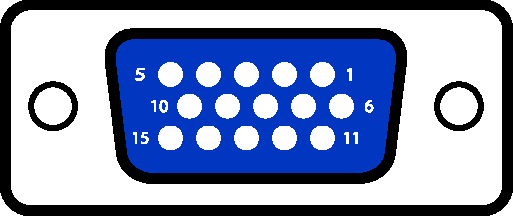
\includegraphics[width=6cm]{figs/DE15_Connector_Pinout.pdf}
  \vspace{1em}\par

  \zebra
  \begin{tabular}{rlll}
    Pin & Standard VGA & CFT VDU \\
    \hline
    1  & Red video & Red video \\
    2  & Green video & Green video \\
    3  & Blue video & Blue video \\
    4  & ID2/Reserved & Not connected \\
    5  & Ground & Ground \\
    6  & Red return & Analogue ground \\
    7  & Green return & Analogue ground \\
    8  & Blue return & Analogue ground \\
    9  & Key/+5V~DC & +5V~DC \\
    10 & Ground & Ground \\
    11 & ID0/Reserved & Not connected \\
    12 & ID1/SDA & Not connected \\
    13 & Horizontal sync & Horizontal sync \\
    14 & Vertical sync & Vertical sync \\
    15 & ID3/SCL & Not connected \\
    \hline
  \end{tabular}
  \caption[VGA Connector Pin-Out]{\label{fig:vdu-vga-pinout}VGA Connector
    pin-out. This is a view of the mating side of a VGA socket. The \ps{ID0–3}
    signals are obsolete and have been replaced (on a conformant VGA) with an
    I²C two-wire interface to transfer monitor parameters to the host. This is
    ignored on the CFT. The ‘key’ pin was missing on original VGAs to allow
    socket keying, but now carries 5V power.}
\end{figure*}

\begin{figure}
 \centering
 % -*- latex -*-
\documentclass[class=memoir,border=200pt]{standalone}
% -*- latex -*-

%%%%%%%%%%%%%%%%%%%%%%%%%%%%%%%%%%%%%%%%%%%%%%%%%%%%%%%%%%%%%%%%%%%%%%%%%%%%%%%
%%
%% PACKAGES
%%
%%%%%%%%%%%%%%%%%%%%%%%%%%%%%%%%%%%%%%%%%%%%%%%%%%%%%%%%%%%%%%%%%%%%%%%%%%%%%%%

\usepackage{ifxetex}
\usepackage{graphicx}

\usepackage{verbatim}
\usepackage{ifthen}
\usepackage{float}
\usepackage{floatflt}
\usepackage{lipsum}
\usepackage{layout}
\usepackage{calc}
\usepackage{rotating}
\usepackage{array}
\usepackage{color}
\usepackage[table]{xcolor}
\usepackage[includefoot]{geometry}

% Conditional packages
\ifxetex
  % Load fontspec and set fonts
  \usepackage{fontspec}
  \setmainfont{Minion Pro}
  \setsansfont{Myriad Pro}
  \setmonofont[]{Inconsolata}

  \usepackage{pdftricks}
  \usepackage{pdfpages}

  \def\HCode#1{}

\else
  \newcounter{Hfootnote}
  \newcommand\fontspec[1]{}
  %\usepackage[main=english,greek]{babel}
  \usepackage[utf8]{inputenc}
  \usepackage{newunicodechar}
  \newunicodechar{®}{\HCode{&reg;}}
  \newunicodechar{µ}{\HCode{&mu;}} % ‘micro’ (from latin-1 plane)
  \newunicodechar{μ}{\HCode{&mu;}} % mu (from Greek plane)
  \newunicodechar{–}{--}
  \newunicodechar{—}{---}
  \newunicodechar{×}{\ensuremath{\times}}
  \newunicodechar{°}{\HCode{&deg;}}
  \newunicodechar{±}{\HCode{&plusm;}}
  \newunicodechar{Ω}{\ensuremath{\Omega}}
  \newunicodechar{÷}{\ensuremath{\div}}
  %\newunicodechar{²}{\HCode{&sup2;}}
  \newunicodechar{²}{*2*}
  \newunicodechar{¼}{\HCode{&\#188;}}
  \newunicodechar{½}{\HCode{&\#189;}}
  \newunicodechar{≤}{\HCode{ &le; }}
  \newunicodechar{≥}{\HCode{ &ge; }}
  \newunicodechar{≠}{\HCode{ &ne; }}
\fi

%%%%%%%%%%%%%%%%%%%%%%%%%%%%%%%%%%%%%%%%%%%%%%%%%%%%%%%%%%%%%%%%%%%%%%%%%%%%%%%
%%
%% TABLES
%%
%%%%%%%%%%%%%%%%%%%%%%%%%%%%%%%%%%%%%%%%%%%%%%%%%%%%%%%%%%%%%%%%%%%%%%%%%%%%%%%

\renewcommand*\arraystretch{1.25}
\newcolumntype{P}[1]{>{\raggedright\arraybackslash}p{#1}}


%%%%%%%%%%%%%%%%%%%%%%%%%%%%%%%%%%%%%%%%%%%%%%%%%%%%%%%%%%%%%%%%%%%%%%%%%%%%%%%
%%
%% FIGURE DRAWING WITH PGF/TIKZ
%%
%%%%%%%%%%%%%%%%%%%%%%%%%%%%%%%%%%%%%%%%%%%%%%%%%%%%%%%%%%%%%%%%%%%%%%%%%%%%%%%

\ifxetex
  \usepackage{pgf}
  \usepackage{tikz}
  \usepackage{rotating}
  \usepackage[absolute]{textpos}

  %\usetikzlibrary{arrows,positioning,automata,shadows,fit,shapes,counters}
  \usetikzlibrary{arrows,positioning,automata,shadows,fit,shapes,patterns}
  \usetikzlibrary{shadows.blur}
  %\usetikzlibrary{external}
  %\tikzexternalize[prefix=tikz/]
  %\tikzset{external/system call={xelatex \tikzexternalcheckshellescape -halt-on-error -interaction=batchmode -jobname "\image" "\texsource"}}
  \usepackage{standalone}

  \usepackage{tikz-timing}[2009/07/28]
  \usetikztiminglibrary{either}[2009/07/28]
  \tikzset{>=latex}
  \tikzset{timing/z/.append style={black},}
  \tikzset{timing/.append style={x=1ex, y=2ex, line cap=round, line join=round, line width=1.3pt}}
  \tikzset{timing/slope=0.33}
  \tikzstyle{semithick}=[line width=1pt]
  \tikzstyle{heavy}=[line width=2pt]
  \tikzstyle{heavy outline}=[line width=3.5pt]
  \tikzstyle{plot line}=[line width=4pt]
  \tikzstyle{arrow}=[semithick]
  \tikzstyle{thick arrow}=[heavy]
  \tikzstyle{thick outline arrow}=[thick arrow, heavy outline, color=white, draw opacity=0.8]
  \tikzstyle{help lines}=[dotted, line width=0.5pt]
  \tikzstyle{col1}=[draw=p1,fill=p1!60]
  \tikzstyle{col2}=[draw=p2,fill=p2!60]
  \tikzstyle{col3}=[draw=p3,fill=p3!60]
  \tikzstyle{col4}=[draw=p4,fill=p4!60]
  \tikzstyle{col5}=[draw=p5,fill=p5!60]
  \tikzstyle{col6}=[draw=p6,fill=p6!60]
  \tikzstyle{dropshadow}=[] % shade,blur shadow={shadow blur steps=5, shadow blur extra rounding=1.3pt}]
  \tikzset{fsmstate/.style={state,rectangle,rounded corners,dropshadow,minimum width=10em,line width=1pt}}
  % Create a hatch pattern
  \newlength{\hatchspread}
  \newlength{\hatchthickness}
  % declaring the keys in tikz
  \tikzset{hatchspread/.code={\setlength{\hatchspread}{#1}},
           hatchthickness/.code={\setlength{\hatchthickness}{#1}}}
  \tikzset{hatchspread=3pt,
           hatchthickness=0.4pt}
  \pgfdeclarepatternformonly[\hatchspread,\hatchthickness]% variables
     {hatch}% name
     {\pgfqpoint{-2\hatchthickness}{-2\hatchthickness}}% lower left corner
     {\pgfqpoint{\dimexpr\hatchspread+2\hatchthickness}{\dimexpr\hatchspread+2\hatchthickness}}% upper right corner
     {\pgfqpoint{\hatchspread}{\hatchspread}}% tile size
     {% shape description
      \pgfsetlinewidth{\hatchthickness}
      \pgfpathmoveto{\pgfqpoint{0pt}{\hatchspread}}
      \pgfpathlineto{\pgfqpoint{\dimexpr\hatchspread+0.15pt}{-0.15pt}}
      \pgfusepath{stroke}
     }
\fi


%%%%%%%%%%%%%%%%%%%%%%%%%%%%%%%%%%%%%%%%%%%%%%%%%%%%%%%%%%%%%%%%%%%%%%%%%%%%%%%
%%
%% HYPERREF
%%
%%%%%%%%%%%%%%%%%%%%%%%%%%%%%%%%%%%%%%%%%%%%%%%%%%%%%%%%%%%%%%%%%%%%%%%%%%%%%%%

\makeatletter
\@ifpackageloaded{standalone}{}{
  \ifxetex
    \usepackage[CJKbookmarks,bookmarks=true,bookmarksopen=true,pdfpagelabels,pdfstartpage=1]{hyperref}
  \else
    \usepackage[tex4ht]{hyperref}
  \fi
}

\let\old@part\part
\renewcommand\part[1]{%
  \setcounter{chapter}{0}%
  \old@part{#1}%
}
%\renewcommand*{\theHchapter}{\thepart.\thechapter}
\makeatother


%%%%%%%%%%%%%%%%%%%%%%%%%%%%%%%%%%%%%%%%%%%%%%%%%%%%%%%%%%%%%%%%%%%%%%%%%%%%%%%
%%
%% INDEX AND GLOSSARY
%%
%%%%%%%%%%%%%%%%%%%%%%%%%%%%%%%%%%%%%%%%%%%%%%%%%%%%%%%%%%%%%%%%%%%%%%%%%%%%%%%

\usepackage{makeidx}
% Glossaries
\usepackage[acronym]{glossaries}
%\makeindex
%\makeglossaries
% -*- latex -*-

\renewcommand\glspostdescription{}

\newcommand\newglossaryabbr[3]{%
  \newglossaryentry{abbr#1}{name=\glslink{#1}{#2}, text={#2}, description={#3}}
  \newacronym[description={\glslink{abbr#1}{#2}}]{#1}{#1}{#2}
}

\newglossaryentry{IBUS}{name=IBUS,
  description={
  Internal Bus: the single, internal 16-bit bus of the CFT processor.
  }}
  
\newglossaryentry{Data Bus}{name=Data Bus, description={ A
    16-bit bus used to move data between the processor and
    peripherals.  }}
  
\newglossaryentry{Address Bus}{name=Address Bus, description={A
    16-bit bus used to select a peripheral nor memory location to
    access.}}
  
\newglossaryentry{Video Display Unit}{name=Video Display Unit,
  description={ Video Display Unit (VDU): a device that drives a
    display monitor to show character or graphics data on a
    screen. Often also contains one or more input devices (keyboard,
    mouse).}}
  
\newglossaryentry{von Neumann architecture}{name=Von Neumann architecture,
  description={ Named after the work of
    John von Neumann, the von Neumann architecture is a ‘modern’
    computer architecture that includes a register file, arithmetic
    and logic units, memory and input/output, and uses the same
    storage for programs and data.}}

\newglossaryentry{stored program computer}{name=Stored program computer,
  description={ A type of computer that
    uses the same storage for programs and data. All modern computers
    are stored program computers, allowing self-modification of their
    programs. Early designs and many modern microcontrollers stored
    programs and data in separate media, and did not or could not
    treat programs as data.}}

\newglossaryabbr{ALU}{Arithmetic/Logic Unit}{Describe this!}
\newglossaryabbr{ISR}{Interrupt Service Routine}{Describe this!}
\newglossaryentry{UART}{name=UART, description={
    Short for Universal Asynchronous Receiver/Transmitter. UARTs are
    devices that handle asynchronous serial communications such as RS-232, RS-485 or USB.
    }
}
%% \newglossaryentry{alu}{name=\glslink{ALU}{Arithmetic/Logic Unit}, text=Arithmetic/Logic Unit,
%%   description={TODO}}
%% \newacronym[description={\glslink{alu}{Arithmetic/Logic Unit}}]{ALU}{ALU}{Arithmetic/Logic Unit}

\newacronym{SBU}{SBU}{Skip/Branch Unit}

\newacronym{AGL}{AGL}{Address Generation Logic}

\newglossaryentry{DEB}{name=DEB, description={
    Designation of the CFT Debugging/Testing board, a peripheral that
    allows remote control and testing of the computer and its
    peripherals in the style of a virtual front panel. The DEB board
    is discussed in~\ccf{chap:deb}.
}}

\newglossaryentry{VDU}{name=VDU, description={ Video Display
    Unit. Designation of the CFT graphic card and keyboard
    controller. The VDU board is discussed in~\ccf{chap:vdu}.  }}

\newglossaryentry{MSB}{name=MSB, description={
    Most Significant Bits. Usually used to refer to the upper eight bits of a CFT word.
}}
\newglossaryentry{LSB}{name=LSB, description={
    Least Significant Bits. Usually used to refer to the lower eight bits of a CFT word.
}}

\newglossaryentry{NYBBLE}{name=Nybble, description={Sometimes
    nibble. A four-bit quantity, represented as a single hexadecimal
    digit.
}}

% \newacronym{MCU}{MCU}{Micro-Controller Unit}

\newglossaryabbr{MCU}{Micro-Controller Unit}{A single-chip device
  containing a simple microprocessor, general purpose input/output,
  serial input/output, timers, and other useful devices.}

\newacronym{USB}{USB}{Universal Serial Bus}

\newacronym{GPIO}{GPIO}{General-Purpose Input/Output}

\newglossaryentry{Verilog}{name=Verilog,
  description={
    One of the two major hardware
    description languages, the other being VHDL. In the CFT project,
    Verilog is used to perform 74xxx chip-level simulation and
    verification of the CFT processor.
}}

\newglossaryentry{I2C}{name=I²C, description={A two-wire, open-drain
    bus, often used for communication between \gls{MCU}s and
    peripheral chips, including EEPROMs and sensors. For more
    information, please consult
    \url{http://en.wikipedia.org/wiki/I2C}.}}

\newglossaryentry{data stack}{name=Data Stack,
  description=To Do}

\newglossaryentry{postfix}{name=postfix,
  description=To Do}

\newglossaryentry{stack effect comment}{name=stack effect comment,
  description=To Do}

\newglossaryentry{Wait State}{name=Wait State, 
  description={An additional state added to the processor state machine
  to accommodate slow devices. External devices signal their need for a
  wait state to the processor using an appropriate procotol. The
  processor then enters the Wait State and does not leave until the
  device is ready. The processor performs no action during this time,
  hence the name.}}


\newglossaryentry{Twos Complement}{name=Two's Complement,
  description={Currently the most popular means of representing signed
    integers in binary. For a bit width $n$, non-negative numbers $0 \leq
    x < 2^{n-1}$ are represented as unsigned $n$-bit binary
    integers. Negative numbers $-2^{n-1} \leq x < 0$ are represented in
    the form $2^n - x$, with the most significant bit set. On the CFT,
    with $n=16$, this provides a signed range of $[-32,768,
      32,767]$. Two's complement has many useful mathematical
    properties: only one representation of zero, the most significant
    bit also acts as a sign bit, and both addition and subtraction can
    be performed by the same circuitry. For a full discussion, please refer
    to \url{http://en.wikipedia.org/wiki/Two's\_complement}.  }}

\newglossaryentry{Assembly}{name=Assembly, description={A symbolic form of
    \gls{machine code}, meant to be used by humans. Some architectures,
    including the CFT, have simple machine code that can be learned in minutes,
    but the human brain deals better with symbols. Assembly languages also
    provide productivity enhancing features like comments, labels, macros,
    simple arithmetic for literals, and other such facilities. The CFT
    Assembler provides all of these facilities.  }}

\newglossaryentry{DIP}{name=DIP, description={Dual In-line Package, the
    most common integrated circuit package until the introduction of
    Surface Mount Technology: DIP chips have two rows of pins, with pins
    set at distances of 2.54~mm (0.1~inch).
}}

\newglossaryentry{PLCC}{name=PLCC, description={Plastic Leaded Chip
    Carrier, a square surface mount chip packaging easily adapted to
    2.54mm grids by means of suitable IC sockets. The CFT uses
    numerous PLCC chips to save board space and because they offer
    more choice of chips, and thus better value for money. All CFT
    PLCC packages are either Flash devices or UARTs.}}

\newglossaryentry{MEM}{name=MEM, description={ Designation of the
    memory board, which, depending on construction details provides up
    to 512 or 1,024 kWords of RAM and/or ROM. The MEM board is
    discussed in~\ccf{chap:mem}.
}}

\newglossaryentry{MBU}{name=MBU, description={Designation of the
    Memory Banking Unit. This was originally slated to be a separate
    peripheral, but has become so important to the project that it is
    now considered to be part of the processor, and constructed as
    such. The MBU breaks memory space in logical and physical
    addresses, and allows the processor's limited 64 kWord address
    space to be expanded to a 21 bit, 2,048 kWord address space using
    memory banking techniques. More details may be found in
    \ccf{chap:mbu}.  }}

\newglossaryentry{Interrupt Service Routine}{name=Interrupt Service Routine (ISR),
  description={TO DO}}

\newglossaryentry{Page}{name=Page, description={The CFT instruction set allows
    for a 10-bit operand, which allows instructions to address up to
    $2^{10}=1024$ locations. This 1,024-word range is known as a page. The CFT
    address space contains 64 such 1 kWord pages. \gls{Page Zero} at addresses
    \hex{0000}–\hex{03FF} has special significance in the programming model, as
    discussed in~\cf{sec:memory-space}.
 }}

\newglossaryentry{Page Zero}{name=Page Zero, description={Page Zero occupies
    the first 1,024 addresses (\hex{0000}–\hex{03FFF}) of the memory address
    space. It is used to simulate 1,024 registers, global variables or
    constants accessible from anywhere in memory. Addresses
    \hex{0080}–\hex{00FF} are autoindex locations: they increment when accessed
    in \gls{Indirect Mode}.}}

\newglossaryentry{Addressing Mode}{name=Addressing Mode, description={An
    addressing mode is the method in which an instruction operand is
    interpreted. The CFT can treat operands as literal values (\gls{Literal
      Mode}), addresses of data (\gls{Direct Mode}), or addresses of addresses
    of data (\gls{Indirect Mode}), similar to pointersin high-level languages
    such as C and Pascal. Addressing modes are discussed
    in~\cf{sec:addressing-modes}}.}

\newglossaryentry{Indirect Mode}{name=Indirect Mode, description={An addressing
    mode where an instruction operand identifies the memory location which
    contains the address of the data to access. Compare \gls{Direct
      Mode}. Addressing modes are discussed in~\cf{sec:addressing-modes}.}}

\newglossaryentry{Direct Mode}{name=Direct Mode, description={An addressing
    mode where an instruction operand identifies the memory location of the
    data to access. Compare \gls{Indirect Mode}. Addressing modes are discussed
    in~\cf{sec:addressing-modes}.}}

\newglossaryentry{Literal Mode}{name=Literal Mode, description={An addressing
    mode where an instruction operand identifies the memory location of the
    data to access. Compare \gls{Indirect Mode}. Addressing modes are discussed
    in~\cf{sec:addressing-modes}.}}

\newglossaryentry{register}{name=Register, description={ A data storage device
    inside a processor. Registers are usually faster than memory, and so are
    used to store intermediate results. In many architectures, notably
    \glspl{ABA}, the only way for the processor to
    manipulate data is to transfer it to a register, operate on the register,
    then transfer it back to its intended location. CFT registers are discussed
    in~\cf{sec:registers}.}}

\newglossaryentry{Accumulator}{name=Accumulator, description={The main
    \gls{register} in an \gls{ABA}. Data must be transferred to the Accumulator
    before it can be operated on by the processor. In the CFT, the Accumulator
    is the only such general purpose register available. The term comes from
    the days of tabulating machines, which used accumulators to accumulate
    (sum) numbers. The Accumulator is designated ‘\AC’ on the CFT. Its hardware
    design is discussed in~\cf{sec:major-registers} and its operation from a
    programmer's point of view is discussed in~\cf{sec:accumulator}.}}

\newglossaryabbr{ABA}{Accumulator-Based Architecture}{A processor architecture
  built around a single (or in some cases, a few) accumulators. Most early
  computers followed this design because of its simplicity, and the CFT does
  too. Having a single register draastically simplifies the instruction format,
  too: from a two-operand instruction format (source, destination), we move to
  a single operand (source or destination). The other operand is always the
  accumulator.  }

\newglossaryentry{nybble}{name=Nybble, description={(sometimes nibble)
    A 4-bit quantity, corresponding to one hexadecimal digit, half a
    byte, or one quarter of a CFT \gls{Word}.}}

\newglossaryentry{Word}{name=Word, description={One CFT Word is a
    16-bit quantity. CFT memory and I/O accesses transfer exactly one
    word each. CFT instructions are also one Word wide. This is not to
    be confused with the Forth concept of a \gls{word} (an identifier).}}

\newglossaryentry{word}{name=Word, description={A Forth word is any
    sequence of non-whitespace characters that is not a number. This
    is not to be confused with the more common concept of the
    \gls{Word} as a numeric datatype.}}

\newglossaryentry{machine code}{name=Machine code, description={Machine code is
    the native language of every processor, where machine instructions and data
    are represented in binary. Machine code is easy for the computer to
    process, but humans find it useful to apply abstraction layers to it: data
    are represented in other bases (octal, decimal and hexadecimal being the
    most common), and symbolic instruction names (rather than binary
    instruction numbers) are used. This set of abstractions is \gls{Assembly}
    language.}}

\newglossaryentry{disk label}{name=Disk Label, description={ A disk label
    stores information about a storage device (not always a disk), including a
    magic number to help detect the block, some optional boot code, and
    definitions for one to sixteen \glspl{disk slice} (partitions). The disk
    label always resides in the first block of a device. The best-known disk
    label format is the MS-DOS Master Boot Record, MBR. The CFT's disk label is
    discussed in~\cf{sec:disk-label}.}}

\newglossaryentry{disk slice}{name=Disk Slice, description={Part of a disk intended to
    hold a \gls{filesystem} or other data. Disks are sliced to make them easier
    to manage, so different operating systems can be used, to control the size
    of stored data, and to avoid corruption in one filesystem destroying all
    data. In the MS-DOS world, slices are known as ‘partitions’, and the
    \gls{disk label} is known as a ‘partition table’ or ‘Master Boot Record’
    depending whether it resides on a data disk or bootable disk. The CFT's
    slice scheme is discussed in~\cf{sec:disk-slices}}.}

\newglossaryentry{filesystem}{name=Filesystem, description={ A large data
    structure used to view a storage medium as a hierarchical collection of
    data objects called files. The filesystem abstracts the natural
    array-of-blocks structure of the storage medium, and provides the user with
    an interface for creating, reading and otherwise operating on files by
    their name, location and other attributes. Files can be larger than the
    natural block size, and this is again handled transparently by the
    filesystem code. The CFT's filesystem is described in~\cf{sec:fs}}}

\newglossaryabbr{VD}{Volume Directory}{A data structure
  describing a CFT \gls{filesystem}. Comparable to a Unix filesystem
  superblock. The VDD is the exact same data structure as a
  \gls{DD}. The difference is in the magic number and the contents of
  the first directory slot (the header), which contains a volume
  header structure.}

\newglossaryabbr{DD}{Directory Descriptor}{A data structure describing
  a directory in a CFT \gls{filesystem}.}

\newglossaryentry{block pointer}{name=Block Pointer, description={A
    32-bit value (\gls{MSB} first) denoting the number of a filesystem
    block. A filesystem's first block is block \hex{00000000}.}}

\newglossaryabbr{DH}{Directory Header}{A data structure describing a
  CFT directory. This is the first entry of a \gls{DD}.}

\newglossaryabbr{OOP}{Object Oriented Programming}{A programming
  paradigm where data and code are bundled together in data structures
  called objects. Programs are built based on the interactions and
  interrelations of these objects.}

\newglossaryentry{descriptor}{name=Descriptor, description={In the CFT Filesystem, a data structure
    that holds metadata on an object in the CFT filesystem. Descriptors share
    some common metadata (e.g. filenames, flags, creation time and date). They
    are located inside container objects (volumes and directories). Containers
    and descriptors are discussed in~\cfp{sec:fs-containers}.}}

\newglossaryentry{volume}{name=Volume, description={A \gls{disk slice} which
    has been structured according to the CFT Filesystem. In \gls{OOP} terms, a
    volume is the object (instance) and the CFT Filesystem is the class.}}

\newglossaryentry{container}{name=Container, description={In the CFT
    Filesystem, a data structure that contains other filesystem objects. Entire
    filesystem \glspl{volume} are containers, and so are directories. Each
    container owns a maximum number of \glspl{descriptor}, identifying the
    contained objects. Once this limit is reached, continuation blocks are
    allocated for the container. These continuation blocks form a doubly linked
    list. Containers are discussed in~\fcf{sec:fs-containers}.}}

\newglossaryabbr{PEL}{Picture Element}{The smallest addressable
  picture element of a display mode. A PEL is usually a block of
  multiple pixels.}

\newglossaryabbr{MTBF}{Mean Time Between Failures}{The average life
  expectancy of a device.}

\newglossaryentry{codepoint}{name=Codepoint, description={A number
    identifying a character within a character set. For example, in
    the ASCII set, codepoint 65 is the character ‘A’.}}

\newglossaryabbr{SDRAM}{Synchronous Dynamic Random Access Memory}{A
  type of modern dynamic RAM that operates using a clock, not
  asynchronously like original DRAMs. The memory contains a command
  pipeline, because data appears on the bus two to three clock ticks
  after a read is signalled. Multiple reads are pipelined, making the
  memory very fast for many use patterns.}

\newglossaryabbr{SRAM}{Static Random Access Memory}{A type of
  relatively low-density memory that trades off capacity and price for
  speed and interface simplicity. SRAMs do not need to be refreshed
  and are faster than similar dynamic RAMs.}

\newglossaryentry{extended instruction}{name=Instruction!Extended,
  description={An address in I/O space that provides side effects
    useful enough to be seen as extending the processor's instruction
    set. They are usually aliases of single \asm{IN}, \asm{OUT} or
    \asm{IOT} instructions.}}

\newglossaryabbr{SR}{Switch Register}{A 16-bit read-only register that
  provides the value of the 16 data entry switches on the front
  panel.}

\newglossaryabbr{DSR}{DIP Switch Register}{A 12 to 16-bit read-only
  register driven by a bank of DIP switches on the Front Panel
  Controller board. The DSR can be used to set non-volatile prefrences
  for the computer's early boot.}

\newglossaryabbr{MFD}{Multi-Function Display}{A bank of 16 lights on
  the front panel which can display a user-selectable register. The
  user can elect to show the value of the Data Register, Output
  Register, or the 15-bit microcode store address. A switch on the
  front panel is used to do this.}

%\newcommand\gls[1]{#1}
%\newcommand\glsresetall{}
\ifxetex
  \glsSetCompositor{-}
  \renewcommand{\delimR}{–}
\fi


%%%%%%%%%%%%%%%%%%%%%%%%%%%%%%%%%%%%%%%%%%%%%%%%%%%%%%%%%%%%%%%%%%%%%%%%%%%%%%%
%%
%% LISTINGS OF THINGS
%%
%%%%%%%%%%%%%%%%%%%%%%%%%%%%%%%%%%%%%%%%%%%%%%%%%%%%%%%%%%%%%%%%%%%%%%%%%%%%%%%

% Lists of things (memoir already includes this if running XeTeX)
\ifxetex
  \relax
\else
  \usepackage{tocloft}
\fi


% Listings
\usepackage{minted}
\newminted{deb}{fontsize=\small}
\newminted{cftasm}{fontsize=\small}
\newminted{c}{fontsize=\small}
\newminted{forth}{fontsize=\small}
\newminted{intr}{fontsize=\small}
\newminted{mcasm}{fontsize=\small}
\newmintedfile{mcasm}{linenos=true,fontsize=\small}

\ifxetex
  \relax
\else

% Modify the minted way of invoking pygmentize if running with
% HTLatex. We'll be converting listings DIRECTLY to HTML and importing
% them into the TeX4ht output with specials.
  \makeatletter
  \newcounter{minted@temp}
  \renewcommand\minted@pygmentize[2][\jobname.pyg]{
    \stepcounter{minted@temp}
    \def\minted@cmd{pygmentize -l #2 -f html -F tokenmerge
      \minted@opt{gobble} \minted@opt{texcl} \minted@opt{mathescape}
      \minted@opt{startinline} \minted@opt{funcnamehighlighting}
      \minted@opt{linenos} -P "verboptions=\minted@opt{extra}"
      -o \jobname-\arabic{minted@temp}.out.pyg #1}
    \immediate\write18{\minted@cmd}
    % Remove kludgy markup hints (four or more @)
    \immediate\write18{sed -i -e s/@@@@//g \jobname-\arabic{minted@temp}.out.pyg}
    % For debugging, uncomment:
    %\immediate\typeout{\minted@cmd}
    \ifthenelse{\equal{\minted@opt@bgcolor}{}}
     {}
     {\begin{minted@colorbg}{\minted@opt@bgcolor}}
     \HCode{<div class="minted #2">}
     \special{t4ht*<\jobname-\arabic{minted@temp}.out.pyg} % Import the HTML output
     \HCode{</div>}
    \ifthenelse{\equal{\minted@opt@bgcolor}{}}
     {}
     {\end{minted@colorbg}}
    %\DeleteFile{\jobname.out.pyg}
  }
  \makeatother
\fi


% Old-style listings
\usepackage{listings}
\lstset{%
  xleftmargin=35pt,
  xrightmargin=5pt,
  basicstyle={\ttfamily},
  backgroundcolor=\color{cfthl!25},
  rulecolor=\color{cfthl!25},
  framesep=5pt,
  rulesep=5pt,
  frame=tlrb,
  framexleftmargin=10pt,
  flexiblecolumns=true,
  keepspaces=true,
  numbers=left,
  numbersep=5pt,
  numberstyle={\scriptsize\sffamily\color{cftlight}}
}


%%%%%%%%%%%%%%%%%%%%%%%%%%%%%%%%%%%%%%%%%%%%%%%%%%%%%%%%%%%%%%%%%%%%%%%%%%%%%%%
%%
%% COLOURS
%%
%%%%%%%%%%%%%%%%%%%%%%%%%%%%%%%%%%%%%%%%%%%%%%%%%%%%%%%%%%%%%%%%%%%%%%%%%%%%%%%

\definecolor{r0}{rgb}{0.33, 0.1, 0.1}
\definecolor{r1}{rgb}{1, 0.3, 0.3}

\definecolor{g0}{rgb}{0.1, 0.33, 0.1}
\definecolor{g1}{rgb}{0.3, 1, 0.3}

\definecolor{cftdark}{cmyk}{0,0.42,0.72,0.84}
\definecolor{cftoutline}{cmyk}{0,0.43,0.72,0.53}
\definecolor{cftlight}{cmyk}{0,0.43,0.72,0.22}
\definecolor{cfthl}{rgb}{.89,.698,.529}

\definecolor{darkblue}{RGB}{0,0,128}
\definecolor{caution}{RGB}{192,0,0}

% Graph colours

\definecolor{p1}{rgb}{0.863, .729, .318} % dcb951
\definecolor{p2}{rgb}{.792, .514, .251}  % c98340
\definecolor{p3}{rgb}{.667, .314, .176}  % aa502c
%\definecolor{p4}{rgb}{.475, .102, .098}
\definecolor{p4}{rgb}{.675, .239, .239}  % ac3d3b
\definecolor{p5}{rgb}{.435, .443, .267}  % 8e9158
\definecolor{p6}{rgb}{.345, .427, .568}  % 586d91


% End of file.


\begin{document}%
%\tikzexternaldisable%
\begin{tikzpicture}%

  \def\w{55mm}
  \def\h{50mm}
  \def\p{10mm}
  \def\step{10mm}
  \def\gstep{2.5mm}
  \def\ia{\p}
  \def\ib{\p+\step}
  \def\ic{\p+2*\step}
  \def\id{\h-\p}

  \draw[draw opacity=0,fill=cfthl!25] (0,\ia) -- (\ia,\ia) -- (\id, \id) -- (\w,\id) -- (\w,\ia) -- (0,\ia);

  \begin{scope}
    \clip (0,0) -- (\w,0) -- (\w,\h) -- (0,\h) -- (0,0);
    \begin{scope}[xshift=\p-\step,yshift=\p-\step]
      \draw[step=\gstep,color=cfthl!90] (0,0) grid (2*\w,2*\h);
    \end{scope}
  \end{scope}
  %\draw[heavy,color=cfthl!90] (0,\h-\p) -- (\w,\h-\p);

  \foreach \y in {\ia, \ib, \ic, \id} {
    \begin{scope}[yshift=\y]
      \draw[thick,color=cfthl!90] (0,0) grid (\w,0);
    \end{scope}
    \begin{scope}[xshift=\y]
      \draw[thick,color=cfthl!90] (0,0) grid (0,\h);
    \end{scope}
  }

  % Vertical axis
  \draw (0,\ia) node[left] {0};
  \begin{scope}[yshift=\ib]\draw (0,0) node[left] {33};\end{scope}
  \begin{scope}[yshift=\ic]\draw (0,0) node[left] {66};\end{scope}
  \begin{scope}[yshift=\id]\draw (0,0) node[left] {100};\end{scope}
  \draw (0,\h) node[left] {\textbf{\% Intensity}};

  % Horizontal axis
  \draw (\ia,0) node[below] {0};
  \begin{scope}[xshift=\ib]\draw (0,0) node[below] {233};\end{scope}
  \begin{scope}[xshift=\ic]\draw (0,0) node[below] {466};\end{scope}
  \begin{scope}[xshift=\id]\draw (0,0) node[below] {700};\end{scope}
  \draw (\w,0) node[below left] {\textbf{mV}};

  % Origin
  \draw[thick,color=cfthl] (0,\p) -- (\w,\p);
  \draw[thick,color=cfthl] (\p,0) -- (\p,\h);
  %\draw[dotted,thick] (0,\p) -- (\w,\p);
  %\draw[dotted,thick] (\p,0) -- (\p,\h);

  % Plot line and bars
  \draw[cfthl,plot line] (0,\ia) -- (\ia,\ia) -- (\id, \id) -- (\w,\id);
  \draw[plot line,color=black] (\ia, \ia) -- (\ib, \ia) -- (\ib, \ib) -- (\ic, \ib) %
  -- (\ic, \ic) -- (\id, \ic) -- (\id, \id);% -- (\w, \id) -- (\w, \ia) -- (\ia, \ia);

  % Frame
  \draw[heavy] (0,0) rectangle (\w, \h);

\end{tikzpicture}%
%\tikzexternalenable%
\end{document}

% End of file.


 \caption[Analogue Channel Ramp]{\label{fig:vdu-analogue-ramp} Analogue channel
   ramp. The black line represents the VDU's ramp superimposed on the ideal
   (analogue) ramp.}
\end{figure}


\subsection{Memory}

The VDU board addresses 17 bits of 16-bit memory, for a 262,144×16 address
space. This memory is implemented as a single static RAM chip with an access
time of 15~ns or below. This memory is used for three distinct memory blocks,
discussed in~\cf{sec:vdu:memory-org}. Using a single chip keeps the design
simpler, reduces the number of bus signals between the CPLD and memory, keeps
signal integrity high by minimising trace lengths, and simplifies routing the
PCB.

\subsection{Indirect Host Access}

Rather than a complex scheme of multiplexed memory accesses, the VDU card
accesses its memory privately. To facilitate host access, it makes available
addresses, data and VDU commands via I/O ports. All communication with the
processor is now achieved via a mere three registers, with additional ones used
to change other variables of the VDU subsystem.

On most computers, a three-port access would constitute a severe
bottleneck. This is certainly the case for architectures with relative indirect
addressing and linear memory. On the CFT, however, accessing a linearly mapped
VDU device would involve performing address arithmetic, storing the result in a
register, then using this value to perform an indirect memory access. This is
precisely the way it is done by the VDU card. Rather than using a memory space
register to store the intermediate address result, a VDU register is used
instead. Commands allow autoincrement of these addresses in the X and/or Y
direction, and reduce the number of CFT instructions needed to perform most
tasks.

Commands are dispatched to the VDU card asynchronously (as far as it is
concerned), and executed at first opportunity. This can be longer than a CFT
write cycle, especially when using repeated commands. Four techniques may be
combined freely to detect if a command has completed execution:

\begin{enumerate}
\item Polling the \port{CRR} register (for repeated commands only). While the
  value is non-zero, the VDU is busy.
\item Polling the \field{GO} bit in the \port{CMD} register.
\item Reading from the \port{HAR} or \port{CPORT} registers will block with
  with zero or more wait states until the VDU host interface is idle. This
  allows synchronous access without the tedium of polling loops.
\item Interrupt-based operation: if configured to do so, the VDU will signal an
  interrupt when command execution has completed.
\end{enumerate}

%% \subsection{Video}

%% The video side of the VDU card is a simple analogue VGA output using either a
%% DB15 socket or a 5×2 header. Analogue output is achieved by using a resistor
%% ladder with two values per channel. This gives six bits of colour, or 64
%% colours.

%% The timing of the video frame is a compromise between easily obtained
%% oscillators for the pixel clock and compatibility with a wide range of display
%% devices. As illustrated in~\pageref{table:vdu-timings}, the mode displa

%% output is timed for approximate (but not match) the timings of VESA CVT 0.26MA, which is a 640×480
%% display mode with a 31.500~MHz pixel clock and a 75~Hz (actually, 74.228~Hz)
%% refresh rate. This mode is guaranteed to work with a very wide range of display
%% devices because it happens to be the same display mode PC compatibles use to
%% display their power on self-test messages.

%% The video card lacks a programmable frame engine, but this particular set of
%% timings can be used to provide a wide range of modes, from 40×30 to
%% 640×480. That is five octaves per dimension, allowing 25 different base modes.

\section{Logical Design}

This section describes the design in greater detail, focusing on how the VDU
behaves from a software perspective. The discussion is based on the high level
block diagram of the VDU, shown in~\fcf{fig:vdu:block-diagram}.

\begin{description}

\li{The display registers} (\cfp{sec:vdu:display-registers}) allow the VDU's
behaviour to be modified by the host.

\li{The frame engine} (\cfp{sec:vdu:frame-engine}) generates a properly timed
image frame, including video enables and sync signals.

\li{The character generator} (\cfp{sec:vdu:chargen}) receives codepoints,
character set information and screen geometry data from the sequencer, and
yields pixel patterns for the video generator.

\li{The colour/attribute engine} (\cfp{sec:vdu:colour-engine}) receives colour
information from the sequencer, combines it with hardware cursor data, and
provides foreground and background colours for the video generator.

\li{The video out circuitry} (\cfp{sec:vdu:video-out}) receives pixel and
colour data and produces RGB colour and synchronisation signals used to
directly drive a monitor.

\li{The display memory} (\cfp{sec:vdu:memory-org}) stores video data received
from the host, and transmitted to the video generation circuitry via the memory
sequencer.

\li{The memory sequencer} (\cfp{sec:vdu:memory-sequencer}) uses the timing
signals from the video engine to co-ordinate memory accesses, reading from
display memory and generating a data stream used to drive the character
generator and colour/attribute engine.

\li{The host interface} (\cfp{sec:vdu:host-interface}) provides an additional
set of host-accessible registers which give the CFT indirect access to display
memory, but make up for it by providing some advanced functionality to offload
common tasks from the processor to the VDU.

\end{description}


\begin{figure}
 \centering
 % -*- latex -*-
\documentclass[class=memoir]{standalone}
% -*- latex -*-
\usepackage{pgf}
\usepackage{tikz}
%\usetikzlibrary{arrows,positioning,automata,shadows,fit,shapes,counters}
\usetikzlibrary{arrows,positioning,automata,shadows,fit,shapes,patterns}
%\usetikzlibrary{external}
%\tikzexternalize[prefix=tikz/]
%\tikzset{external/system call={xelatex \tikzexternalcheckshellescape -halt-on-error -interaction=batchmode -jobname "\image" "\texsource"}}
\usepackage{standalone}

\usepackage{layout}

%\usepackage[tocindentauto]{tocstyle}

%\usepackage[cam,a4,center]{crop}

\hypersetup{
    pdftitle={CFT Minicomputer Programming Guide},
    pdfauthor={Alexios Chouchoulas},
    pdfkeywords={},
    bookmarksnumbered,
    pagebackref=true,
    breaklinks=true,
%    pdfview=FitH,       % Or try pdfstartview={FitV}, This lead to uncorrect bookmarks
    urlcolor=darkblue,
    colorlinks=true,
    citecolor=cftoutline,          %citeref's color
    linkcolor=cftoutline,
        }

\makeindex
\makeglossaries
% -*- latex -*-

\renewcommand\glspostdescription{}

\newcommand\newglossaryabbr[3]{%
  \newglossaryentry{abbr#1}{name=\glslink{#1}{#2}, text={#2}, description={#3}}
  \newacronym[description={\glslink{abbr#1}{#2}}]{#1}{#1}{#2}
}

\newglossaryentry{IBUS}{name=IBUS,
  description={
  Internal Bus: the single, internal 16-bit bus of the CFT processor.
  }}
  
\newglossaryentry{Data Bus}{name=Data Bus, description={ A
    16-bit bus used to move data between the processor and
    peripherals.  }}
  
\newglossaryentry{Address Bus}{name=Address Bus, description={A
    16-bit bus used to select a peripheral nor memory location to
    access.}}
  
\newglossaryentry{Video Display Unit}{name=Video Display Unit,
  description={ Video Display Unit (VDU): a device that drives a
    display monitor to show character or graphics data on a
    screen. Often also contains one or more input devices (keyboard,
    mouse).}}
  
\newglossaryentry{von Neumann architecture}{name=Von Neumann architecture,
  description={ Named after the work of
    John von Neumann, the von Neumann architecture is a ‘modern’
    computer architecture that includes a register file, arithmetic
    and logic units, memory and input/output, and uses the same
    storage for programs and data.}}

\newglossaryentry{stored program computer}{name=Stored program computer,
  description={ A type of computer that
    uses the same storage for programs and data. All modern computers
    are stored program computers, allowing self-modification of their
    programs. Early designs and many modern microcontrollers stored
    programs and data in separate media, and did not or could not
    treat programs as data.}}

\newglossaryabbr{ALU}{Arithmetic/Logic Unit}{Describe this!}
\newglossaryabbr{ISR}{Interrupt Service Routine}{Describe this!}
\newglossaryentry{UART}{name=UART, description={
    Short for Universal Asynchronous Receiver/Transmitter. UARTs are
    devices that handle asynchronous serial communications such as RS-232, RS-485 or USB.
    }
}
%% \newglossaryentry{alu}{name=\glslink{ALU}{Arithmetic/Logic Unit}, text=Arithmetic/Logic Unit,
%%   description={TODO}}
%% \newacronym[description={\glslink{alu}{Arithmetic/Logic Unit}}]{ALU}{ALU}{Arithmetic/Logic Unit}

\newacronym{SBU}{SBU}{Skip/Branch Unit}

\newacronym{AGL}{AGL}{Address Generation Logic}

\newglossaryentry{DEB}{name=DEB, description={
    Designation of the CFT Debugging/Testing board, a peripheral that
    allows remote control and testing of the computer and its
    peripherals in the style of a virtual front panel. The DEB board
    is discussed in~\ccf{chap:deb}.
}}

\newglossaryentry{VDU}{name=VDU, description={ Video Display
    Unit. Designation of the CFT graphic card and keyboard
    controller. The VDU board is discussed in~\ccf{chap:vdu}.  }}

\newglossaryentry{MSB}{name=MSB, description={
    Most Significant Bits. Usually used to refer to the upper eight bits of a CFT word.
}}
\newglossaryentry{LSB}{name=LSB, description={
    Least Significant Bits. Usually used to refer to the lower eight bits of a CFT word.
}}

\newglossaryentry{NYBBLE}{name=Nybble, description={Sometimes
    nibble. A four-bit quantity, represented as a single hexadecimal
    digit.
}}

% \newacronym{MCU}{MCU}{Micro-Controller Unit}

\newglossaryabbr{MCU}{Micro-Controller Unit}{A single-chip device
  containing a simple microprocessor, general purpose input/output,
  serial input/output, timers, and other useful devices.}

\newacronym{USB}{USB}{Universal Serial Bus}

\newacronym{GPIO}{GPIO}{General-Purpose Input/Output}

\newglossaryentry{Verilog}{name=Verilog,
  description={
    One of the two major hardware
    description languages, the other being VHDL. In the CFT project,
    Verilog is used to perform 74xxx chip-level simulation and
    verification of the CFT processor.
}}

\newglossaryentry{I2C}{name=I²C, description={A two-wire, open-drain
    bus, often used for communication between \gls{MCU}s and
    peripheral chips, including EEPROMs and sensors. For more
    information, please consult
    \url{http://en.wikipedia.org/wiki/I2C}.}}

\newglossaryentry{data stack}{name=Data Stack,
  description=To Do}

\newglossaryentry{postfix}{name=postfix,
  description=To Do}

\newglossaryentry{stack effect comment}{name=stack effect comment,
  description=To Do}

\newglossaryentry{Wait State}{name=Wait State, 
  description={An additional state added to the processor state machine
  to accommodate slow devices. External devices signal their need for a
  wait state to the processor using an appropriate procotol. The
  processor then enters the Wait State and does not leave until the
  device is ready. The processor performs no action during this time,
  hence the name.}}


\newglossaryentry{Twos Complement}{name=Two's Complement,
  description={Currently the most popular means of representing signed
    integers in binary. For a bit width $n$, non-negative numbers $0 \leq
    x < 2^{n-1}$ are represented as unsigned $n$-bit binary
    integers. Negative numbers $-2^{n-1} \leq x < 0$ are represented in
    the form $2^n - x$, with the most significant bit set. On the CFT,
    with $n=16$, this provides a signed range of $[-32,768,
      32,767]$. Two's complement has many useful mathematical
    properties: only one representation of zero, the most significant
    bit also acts as a sign bit, and both addition and subtraction can
    be performed by the same circuitry. For a full discussion, please refer
    to \url{http://en.wikipedia.org/wiki/Two's\_complement}.  }}

\newglossaryentry{Assembly}{name=Assembly, description={A symbolic form of
    \gls{machine code}, meant to be used by humans. Some architectures,
    including the CFT, have simple machine code that can be learned in minutes,
    but the human brain deals better with symbols. Assembly languages also
    provide productivity enhancing features like comments, labels, macros,
    simple arithmetic for literals, and other such facilities. The CFT
    Assembler provides all of these facilities.  }}

\newglossaryentry{DIP}{name=DIP, description={Dual In-line Package, the
    most common integrated circuit package until the introduction of
    Surface Mount Technology: DIP chips have two rows of pins, with pins
    set at distances of 2.54~mm (0.1~inch).
}}

\newglossaryentry{PLCC}{name=PLCC, description={Plastic Leaded Chip
    Carrier, a square surface mount chip packaging easily adapted to
    2.54mm grids by means of suitable IC sockets. The CFT uses
    numerous PLCC chips to save board space and because they offer
    more choice of chips, and thus better value for money. All CFT
    PLCC packages are either Flash devices or UARTs.}}

\newglossaryentry{MEM}{name=MEM, description={ Designation of the
    memory board, which, depending on construction details provides up
    to 512 or 1,024 kWords of RAM and/or ROM. The MEM board is
    discussed in~\ccf{chap:mem}.
}}

\newglossaryentry{MBU}{name=MBU, description={Designation of the
    Memory Banking Unit. This was originally slated to be a separate
    peripheral, but has become so important to the project that it is
    now considered to be part of the processor, and constructed as
    such. The MBU breaks memory space in logical and physical
    addresses, and allows the processor's limited 64 kWord address
    space to be expanded to a 21 bit, 2,048 kWord address space using
    memory banking techniques. More details may be found in
    \ccf{chap:mbu}.  }}

\newglossaryentry{Interrupt Service Routine}{name=Interrupt Service Routine (ISR),
  description={TO DO}}

\newglossaryentry{Page}{name=Page, description={The CFT instruction set allows
    for a 10-bit operand, which allows instructions to address up to
    $2^{10}=1024$ locations. This 1,024-word range is known as a page. The CFT
    address space contains 64 such 1 kWord pages. \gls{Page Zero} at addresses
    \hex{0000}–\hex{03FF} has special significance in the programming model, as
    discussed in~\cf{sec:memory-space}.
 }}

\newglossaryentry{Page Zero}{name=Page Zero, description={Page Zero occupies
    the first 1,024 addresses (\hex{0000}–\hex{03FFF}) of the memory address
    space. It is used to simulate 1,024 registers, global variables or
    constants accessible from anywhere in memory. Addresses
    \hex{0080}–\hex{00FF} are autoindex locations: they increment when accessed
    in \gls{Indirect Mode}.}}

\newglossaryentry{Addressing Mode}{name=Addressing Mode, description={An
    addressing mode is the method in which an instruction operand is
    interpreted. The CFT can treat operands as literal values (\gls{Literal
      Mode}), addresses of data (\gls{Direct Mode}), or addresses of addresses
    of data (\gls{Indirect Mode}), similar to pointersin high-level languages
    such as C and Pascal. Addressing modes are discussed
    in~\cf{sec:addressing-modes}}.}

\newglossaryentry{Indirect Mode}{name=Indirect Mode, description={An addressing
    mode where an instruction operand identifies the memory location which
    contains the address of the data to access. Compare \gls{Direct
      Mode}. Addressing modes are discussed in~\cf{sec:addressing-modes}.}}

\newglossaryentry{Direct Mode}{name=Direct Mode, description={An addressing
    mode where an instruction operand identifies the memory location of the
    data to access. Compare \gls{Indirect Mode}. Addressing modes are discussed
    in~\cf{sec:addressing-modes}.}}

\newglossaryentry{Literal Mode}{name=Literal Mode, description={An addressing
    mode where an instruction operand identifies the memory location of the
    data to access. Compare \gls{Indirect Mode}. Addressing modes are discussed
    in~\cf{sec:addressing-modes}.}}

\newglossaryentry{register}{name=Register, description={ A data storage device
    inside a processor. Registers are usually faster than memory, and so are
    used to store intermediate results. In many architectures, notably
    \glspl{ABA}, the only way for the processor to
    manipulate data is to transfer it to a register, operate on the register,
    then transfer it back to its intended location. CFT registers are discussed
    in~\cf{sec:registers}.}}

\newglossaryentry{Accumulator}{name=Accumulator, description={The main
    \gls{register} in an \gls{ABA}. Data must be transferred to the Accumulator
    before it can be operated on by the processor. In the CFT, the Accumulator
    is the only such general purpose register available. The term comes from
    the days of tabulating machines, which used accumulators to accumulate
    (sum) numbers. The Accumulator is designated ‘\AC’ on the CFT. Its hardware
    design is discussed in~\cf{sec:major-registers} and its operation from a
    programmer's point of view is discussed in~\cf{sec:accumulator}.}}

\newglossaryabbr{ABA}{Accumulator-Based Architecture}{A processor architecture
  built around a single (or in some cases, a few) accumulators. Most early
  computers followed this design because of its simplicity, and the CFT does
  too. Having a single register draastically simplifies the instruction format,
  too: from a two-operand instruction format (source, destination), we move to
  a single operand (source or destination). The other operand is always the
  accumulator.  }

\newglossaryentry{nybble}{name=Nybble, description={(sometimes nibble)
    A 4-bit quantity, corresponding to one hexadecimal digit, half a
    byte, or one quarter of a CFT \gls{Word}.}}

\newglossaryentry{Word}{name=Word, description={One CFT Word is a
    16-bit quantity. CFT memory and I/O accesses transfer exactly one
    word each. CFT instructions are also one Word wide. This is not to
    be confused with the Forth concept of a \gls{word} (an identifier).}}

\newglossaryentry{word}{name=Word, description={A Forth word is any
    sequence of non-whitespace characters that is not a number. This
    is not to be confused with the more common concept of the
    \gls{Word} as a numeric datatype.}}

\newglossaryentry{machine code}{name=Machine code, description={Machine code is
    the native language of every processor, where machine instructions and data
    are represented in binary. Machine code is easy for the computer to
    process, but humans find it useful to apply abstraction layers to it: data
    are represented in other bases (octal, decimal and hexadecimal being the
    most common), and symbolic instruction names (rather than binary
    instruction numbers) are used. This set of abstractions is \gls{Assembly}
    language.}}

\newglossaryentry{disk label}{name=Disk Label, description={ A disk label
    stores information about a storage device (not always a disk), including a
    magic number to help detect the block, some optional boot code, and
    definitions for one to sixteen \glspl{disk slice} (partitions). The disk
    label always resides in the first block of a device. The best-known disk
    label format is the MS-DOS Master Boot Record, MBR. The CFT's disk label is
    discussed in~\cf{sec:disk-label}.}}

\newglossaryentry{disk slice}{name=Disk Slice, description={Part of a disk intended to
    hold a \gls{filesystem} or other data. Disks are sliced to make them easier
    to manage, so different operating systems can be used, to control the size
    of stored data, and to avoid corruption in one filesystem destroying all
    data. In the MS-DOS world, slices are known as ‘partitions’, and the
    \gls{disk label} is known as a ‘partition table’ or ‘Master Boot Record’
    depending whether it resides on a data disk or bootable disk. The CFT's
    slice scheme is discussed in~\cf{sec:disk-slices}}.}

\newglossaryentry{filesystem}{name=Filesystem, description={ A large data
    structure used to view a storage medium as a hierarchical collection of
    data objects called files. The filesystem abstracts the natural
    array-of-blocks structure of the storage medium, and provides the user with
    an interface for creating, reading and otherwise operating on files by
    their name, location and other attributes. Files can be larger than the
    natural block size, and this is again handled transparently by the
    filesystem code. The CFT's filesystem is described in~\cf{sec:fs}}}

\newglossaryabbr{VD}{Volume Directory}{A data structure
  describing a CFT \gls{filesystem}. Comparable to a Unix filesystem
  superblock. The VDD is the exact same data structure as a
  \gls{DD}. The difference is in the magic number and the contents of
  the first directory slot (the header), which contains a volume
  header structure.}

\newglossaryabbr{DD}{Directory Descriptor}{A data structure describing
  a directory in a CFT \gls{filesystem}.}

\newglossaryentry{block pointer}{name=Block Pointer, description={A
    32-bit value (\gls{MSB} first) denoting the number of a filesystem
    block. A filesystem's first block is block \hex{00000000}.}}

\newglossaryabbr{DH}{Directory Header}{A data structure describing a
  CFT directory. This is the first entry of a \gls{DD}.}

\newglossaryabbr{OOP}{Object Oriented Programming}{A programming
  paradigm where data and code are bundled together in data structures
  called objects. Programs are built based on the interactions and
  interrelations of these objects.}

\newglossaryentry{descriptor}{name=Descriptor, description={In the CFT Filesystem, a data structure
    that holds metadata on an object in the CFT filesystem. Descriptors share
    some common metadata (e.g. filenames, flags, creation time and date). They
    are located inside container objects (volumes and directories). Containers
    and descriptors are discussed in~\cfp{sec:fs-containers}.}}

\newglossaryentry{volume}{name=Volume, description={A \gls{disk slice} which
    has been structured according to the CFT Filesystem. In \gls{OOP} terms, a
    volume is the object (instance) and the CFT Filesystem is the class.}}

\newglossaryentry{container}{name=Container, description={In the CFT
    Filesystem, a data structure that contains other filesystem objects. Entire
    filesystem \glspl{volume} are containers, and so are directories. Each
    container owns a maximum number of \glspl{descriptor}, identifying the
    contained objects. Once this limit is reached, continuation blocks are
    allocated for the container. These continuation blocks form a doubly linked
    list. Containers are discussed in~\fcf{sec:fs-containers}.}}

\newglossaryabbr{PEL}{Picture Element}{The smallest addressable
  picture element of a display mode. A PEL is usually a block of
  multiple pixels.}

\newglossaryabbr{MTBF}{Mean Time Between Failures}{The average life
  expectancy of a device.}

\newglossaryentry{codepoint}{name=Codepoint, description={A number
    identifying a character within a character set. For example, in
    the ASCII set, codepoint 65 is the character ‘A’.}}

\newglossaryabbr{SDRAM}{Synchronous Dynamic Random Access Memory}{A
  type of modern dynamic RAM that operates using a clock, not
  asynchronously like original DRAMs. The memory contains a command
  pipeline, because data appears on the bus two to three clock ticks
  after a read is signalled. Multiple reads are pipelined, making the
  memory very fast for many use patterns.}

\newglossaryabbr{SRAM}{Static Random Access Memory}{A type of
  relatively low-density memory that trades off capacity and price for
  speed and interface simplicity. SRAMs do not need to be refreshed
  and are faster than similar dynamic RAMs.}

\newglossaryentry{extended instruction}{name=Instruction!Extended,
  description={An address in I/O space that provides side effects
    useful enough to be seen as extending the processor's instruction
    set. They are usually aliases of single \asm{IN}, \asm{OUT} or
    \asm{IOT} instructions.}}

\newglossaryabbr{SR}{Switch Register}{A 16-bit read-only register that
  provides the value of the 16 data entry switches on the front
  panel.}

\newglossaryabbr{DSR}{DIP Switch Register}{A 12 to 16-bit read-only
  register driven by a bank of DIP switches on the Front Panel
  Controller board. The DSR can be used to set non-volatile prefrences
  for the computer's early boot.}

\newglossaryabbr{MFD}{Multi-Function Display}{A bank of 16 lights on
  the front panel which can display a user-selectable register. The
  user can elect to show the value of the Data Register, Output
  Register, or the 15-bit microcode store address. A switch on the
  front panel is used to do this.}


\usepackage{listings}
\lstset{%
  xleftmargin=35pt,
  xrightmargin=5pt,
  basicstyle={\ttfamily},
  backgroundcolor=\color{cfthl!25},
  rulecolor=\color{cfthl!25},
  framesep=5pt,
  rulesep=5pt,
  frame=tlrb,
  framexleftmargin=10pt,
  flexiblecolumns=true,
  keepspaces=true,
  numbers=left,
  numbersep=5pt,
  numberstyle={\scriptsize\sffamily\color{cftlight}}
}




%%%%%%%%%%%%%%%%%%%%%%%%%%%%%%%%%%%%%%%%%%%%%%%%%%%%%%%%%%%%%%%%%%%%%%%%%%%%%%%
%%
%% LISTS OF THINGS
%%
%%%%%%%%%%%%%%%%%%%%%%%%%%%%%%%%%%%%%%%%%%%%%%%%%%%%%%%%%%%%%%%%%%%%%%%%%%%%%%%

%% %%%\addtolength\cftfignumwidth{1.5em}
\makeatletter
%% \addtolength{\cftchapternumwidth}{0.5em}
%% \addtolength{\cftsectionnumwidth}{0.5em}
%% \addtolength{\cftsubsectionnumwidth}{0.5em}
%% \addtolength{\cftfigurenumwidth}{0.5em}
%% \addtolength{\cfttablenumwidth}{0.5em}
\renewcommand*\l@section{\@dottedtocline{1}{1.5em}{2.3em}}
\renewcommand*\l@subsection{\@dottedtocline{2}{3.8em}{3.2em}}
\renewcommand*\l@subsubsection{\@dottedtocline{3}{7.0em}{4.1em}}
\renewcommand*\l@paragraph{\@dottedtocline{4}{10em}{5em}}
\renewcommand*\l@subparagraph{\@dottedtocline{5}{12em}{6em}}
\setcounter{maxsecnumdepth}{3}

%\addtolength{\cftschematicsnumwidth}{1em}
\renewcommand{\@pnumwidth}{3em}
\renewcommand{\@tocrmarg}{4em}
\makeatother

%\newcommand\listalgname{List of Algorithms} 
%\newlistof{alg}{algorithm}

%
% Schematics
%

\newcommand\listschematicname{List of Schematics} 
\newlistof{listofschematic}{los}{\listschematicname}
\newcounter{schematic}
\newcommand{\schematic}[1]{%
  \refstepcounter{schematic}%
  \par\noindent\textbf{Schematic \theschematic. #1}
  \addcontentsline{los}{section}{\protect\numberline{\theschematic}#1}\par%
}
\newcommand\listofschematics\listofschematic

%
% I/O Ports
%

\newcommand\listioportname{List of Input/Output Ports} 
\newlistof{listofioport}{loioport}{\listioportname}
%% \newcommand{\registerioport}[1]{%
%%   \refstepcounter{ioport}%
%%   \addcontentsline{loioport}{section}{\protect\numberline{\ }%
%% }
\newcommand\listofioports\listofioport



\newcommand\caution[1]{\textcolor{caution}{\textbf{#1}}}
%\newcommand\todo[1]{\textcolor{caution}{\bf{TODO: #1}}}

%
% Tasks
%

\newcommand\listtasksname{List of Incomplete Tasks} 
\newlistof{listoftask}{lotasks}{\listtasksname}
\newcounter{task}
\newcommand{\todo}[1]{%
  \refstepcounter{task}%
  {\textcolor{caution}{\textbf{TODO: #1}}}
  \addcontentsline{lotasks}{section}{\protect\numberline{\arabic{task}}To Do: #1}\par%
}
\newcommand{\bug}[2]{%
  \refstepcounter{task}%
  {\textcolor{caution}{\textbf{BUG: #1 #2}}}
  \addcontentsline{lotasks}{section}{\protect\numberline{\arabic{task}}Bug: #1}\par%
}
\newcommand\listoftasks\listoftask

%
% Data structures
%

\newcommand\listdatastructurename{List of Data Structures} 
\newlistof{listofdatastructure}{lods}{\listdatastructurename}
\newcounter{datastructure}
%\newcommand{\datastructure}[1]{%
%  \refstepcounter{datastructure}%
%  \par\noindent\textbf{Data Structure \thedatastructure. #1}
%  \addcontentsline{lods}{section}{\protect\numberline{\thedatastructure}#1}\par%
%}
\newcommand\listofdatastructures\listofdatastructure



%%%%%%%%%%%%%%%%%%%%%%%%%%%%%%%%%%%%%%%%%%%%%%%%%%%%%%%%%%%%%%%%%%%%%%%%%%%%%%%
%%
%% SECTION STYLING
%%
%%%%%%%%%%%%%%%%%%%%%%%%%%%%%%%%%%%%%%%%%%%%%%%%%%%%%%%%%%%%%%%%%%%%%%%%%%%%%%%



%% \usepackage{kpfonts}
\usepackage[explicit]{titlesec}

\counterwithin*{chapter}{part}
\counterwithin*{figure}{chapter}
\counterwithin*{schematic}{chapter}
\counterwithin*{datastructure}{chapter}
\counterwithin*{table}{chapter}

%%%%%%%%%%%%%%%%%%%%%%%%%%%%%%%%%%%%%%%%%%%%%%%%%%%%%%%%%%%%%%%%%%%%%%%%%%%%%%%

\renewcommand\thepart{\Alph{part}}
\cftpagenumbersoff{part}
%\newcommand*\partlabel{}

\makeatletter
\patchcmd{\l@part}{\hss#2}{}{}{}
\makeatother


\renewcommand\partnamefont{\normalfont\sffamily\Huge\scshape}
\renewcommand\partnumfont{\bfseries}
\renewcommand\printparttitle[1]{
  \thispagestyle{empty}
    \begin{tikzpicture}[remember picture,overlay]
      \node[yshift=-\paperheight, draw opacity=0] at (current page.north west)
           {\begin{tikzpicture}[remember picture, overlay]
               \draw[fill=cftlight] (0,0) rectangle
               (\paperwidth,\paperheight);
               \draw[fill=cftoutline] (0,1cm) rectangle
               (\paperwidth,0);
               \node[anchor=east,yshift=0.5\paperheight,xshift=.87\paperwidth,rectangle]
                    {\scalebox{2}{\color{white}\printpartname~\printpartnum}};
                    \node[anchor=east,yshift=0.43\paperheight,xshift=.87\paperwidth,rectangle]
                         {\scalebox{1.5}{\color{white} #1}};
             \end{tikzpicture}
           };
    \end{tikzpicture}
}


\newcommand*\chapterlabel{}
\titleformat{\chapter}
  {\gdef\chapterlabel{}
   \normalfont\sffamily\Huge}
  {\gdef\chapterlabel{\thechapter\ }}{0pt}
  {%
    \setcounter{page}{1}
    \begin{tikzpicture}[remember picture,overlay]
    \node[yshift=-5cm, draw opacity=0] at (current page.north west)
      {\begin{tikzpicture}[remember picture, overlay]
        \draw[fill=cftlight] (0,0) rectangle
          (\paperwidth,5cm);
        \draw[fill=cftoutline] (0,0.25cm) rectangle
          (\paperwidth,0);
        \node[anchor=east,yshift=2cm,xshift=.87\paperwidth,rectangle]
              {\color{white}\chapterlabel#1};
       \end{tikzpicture}
      };
   \end{tikzpicture}
  }
\titlespacing*{\chapter}{0pt}{50pt}{20pt}

\titleformat{\section}
            {\gdef\sectionlabel{}\normalfont\sffamily\Large}
            {\gdef\sectionlabel{\thesection\ }}{0pt}
            {\color{cftoutline}\thesection\quad #1\\
              \titlerule[2pt]
            }[{\vspace{-30pt}\color{cftoutline}\rule{\textwidth}{2pt}}]


\titleformat{\subsection}
  {\gdef\subsectionlabel{}
   \normalfont\sffamily\bfseries\large}
  {\gdef\subsectionlabel{\thesubsection\ }}{0pt}
  {\color{cftoutline}\thesubsection\quad #1}


\titleformat{\subsubsection}
  {\gdef\subsubsectionlabel{}
   \normalfont\sffamily\large}
  {\gdef\subsubsectionlabel{\thesubsubsection\ }}{0pt}
  {\color{cftoutline}#1}


%%%%%%%%%%%%%%%%%%%%%%%%%%%%%%%%%%%%%%%%%%%%%%%%%%%%%%%%%%%%%%%%%%%%%%%%%%%%%%%










%% \titleformat{\paragraph}
%%   {\gdef\chapterlabel{}
%%    \normalfont\bfseries}
%%   {\gdef\chapterlabel{\theparagraph\ }}{0pt}
%%   {\color{cftoutline}#1}



%\geometry{a4paper, hoffset=0in, voffset=-.25in, left=1.5cm, right=1.5cm,
%  top=2.5cm, bottom=2.5cm}
%\geometry{paperwidth=17.5cm, paperheight=23.1cm, hoffset=0in, voffset=-.25in, left=1in, right=1in,
%  top=1in, bottom=1in}
\geometry{a4paper, hoffset=0in, left=1.2in, right=1.2in,
  top=1.2in, bottom=1.2in, includefoot, footskip=40pt}
%\sloppy


% Fonts
%\defaultfontfeatures{Mapping=tex-text}
\setmainfont{Minion Pro}
\setsansfont{Myriad Pro}
\setmonofont[]{Inconsolata}


% Not really used here, but never mind.
\setlength\columnsep{7mm}


% Input our local macro definitions
% -*- latex -*-

\definecolor{caution}{RGB}{192,0,0}

\newcommand\textcond{\fontspec{Myriad Pro Condensed}}

% Primary index entries
\newcommand\pie[1]{\textbf{\hyperpage{#1}}}

% Use hyperlinking when rendering PDFs
\newcommand{\barecf}[1]{\hyperref[#1]{\ref*{#1}}}
\newcommand{\cf}[2][section]{\hyperref[#2]{%
        \ifthenelse{\equal{\pageref*{#2}}{\thepage}}%
        {#1 \ref*{#2}}%
        {#1 \ref*{#2} (p.~\pageref*{#2})}%
}}
\newcommand{\cfp}[2][section]{\hyperref[#2]{%
        \ifthenelse{\equal{\pageref*{#2}}{\thepage}}%
        {#1 \ref*{#2}}%
        {#1 \ref*{#2}, p.~\pageref*{#2}}%
}}
\newcommand{\fcf}[1]{\cf[figure]{#1}}
\newcommand{\fcfp}[1]{\cfp[figure]{#1}}
\newcommand{\tcf}[1]{\cf[table]{#1}}
\newcommand{\tcfp}[1]{\cfp[table]{#1}}
\newcommand{\ccf}[1]{\cf[chapter]{#1}}
\newcommand{\ccfp}[1]{\cfp[chapter]{#1}}
%
\newcommand{\npcf}[2][section]{\hyperref[#2]{#1 \ref*{#2}}}
\newcommand{\appcf}[1]{\cf[appendix]{#1}}
\newcommand{\ecf}[1]{\cf[equation]{#1}}
\newcommand{\algcf}[1]{\cf[algorithm]{#1}}
\newcommand{\npappcf}[1]{\npcf[appendix]{#1}}
\newcommand{\npccf}[1]{\npcf[chapter]{#1}}
\newcommand{\npfcf}[1]{\npcf[figure]{#1}}
\newcommand{\nptcf}[1]{\npcf[table]{#1}}
\newcommand{\npecf}[1]{\npcf[equation]{#1}}
\newcommand{\npalgcf}[1]{\npcf[algorithm]{#1}}

\newcommand\hyperemail[1]{\sffamily\href{mailto:#1}{#1}}
\newcommand\link[1]{\sffamily\href{http://#1}{#1}}
\newcommand\ahref[2]{\sffamily\href{#1}{#2}}

\newcommand\op[1]{{\ttfamily #1}}
\newcommand\fwni[1]{{\ttfamily{#1}}}
\newcommand\fw[1]{\fwni{#1}\index{#1@\protect\fwni{#1}}}
%                           \index{#1@\fwni{#1}|(pie}%

\newcommand\f[1]{{\texttt{#1}}}
\newcommand\hex[1]{\textsf{#1}}
\newcommand\bin[1]{\textsf{#1}}
\newcommand\bitmap[1]{\texttt{#1}}
\newcommand\bus[1]{{#1}}
\newcommand\unit[1]{{#1}}
\newcommand\IBUS{\bus{\gls{IBUS}\index{IBUS}}}
\newcommand\DBUS{\bus{\gls{Data Bus}\index{Data Bus}}}
\newcommand\ABUS{\bus{\gls{Address Bus}\index{Address Bus}}}
\newcommand\ALU{\unit{\gls{ALU}\index{ALU}}}
\newcommand\SBU{\unit{\gls{SBU}\index{SBU}}}
\newcommand\AGL{\unit{\gls{AGL}\index{AGL}}}
\newcommand\register[1]{\textsf{#1}\index{Registers!#1}}
\newcommand\A{\register{AC}}
\newcommand\AC{\A}
\newcommand\Areg{\A}
\newcommand\Lreg{\register{L}}
\newcommand\Ireg{\register{I}}
\newcommand\Zreg{\register{Z}}
\newcommand\Vreg{\register{V}}
\newcommand\Nreg{\register{N}}
\newcommand\AR{\register{AR}}
\newcommand\MAR{\AR}
\newcommand\DR{\register{DR}}
\newcommand\PC{\register{PC}}
\newcommand\IR{\register{IR}}

\newcommand{\asm}[1]{\texttt{#1}}
\newcommand{\instr}[1]{\asm{#1}}
\newcommand{\nsni}[1]{$\overline{\mbox{\textsf{{#1}}}}$}
\newcommand{\ns}[1]{\nsni{#1}\index{#1@{$\protect\overline{\protect\mbox{\textsf{#1}}}$}}}
\newcommand{\psni}[1]{\textsf{#1}}
\newcommand{\ps}[1]{\psni{#1}\index{#1@\psni{#1}}}
\newcommand{\lt}[1]{\textsf{#1}}
\newcommand{\sw}[1]{\textsf{#1\index{Switch, front panel!#1}}}
\newcommand{\HC}[1]{\chip{74HC{#1}}}
\newcommand{\HCT}[1]{\chip{74HCT{#1}}}
\newcommand{\chip}[1]{#1\index{#1}}

\newcommand{\schpt}[1]{#1\textsf{#1}}
\newcommand{\farnell}[1]{#1}

\newcommand\BUS[2]{\ps{#1}$_{\mbox{\scriptsize #2}}$}
\newcommand\nBUS[2]{\ns{#1}$_{\mbox{\scriptsize #2}}$}

\newcommand\UINSTR{\ns{uINSTR18}}
\newcommand\HALT{\ns{HALT}}
\newcommand\END{\ns{END}}
\newcommand\IRQ{\ns{IRQ}}
\newcommand\IRQS{\ns{IRQS}}
\newcommand\IRQn[1]{\nBUS{IRQ}{#1}}
\newcommand\RUNITn[1]{\BUS{RUNIT}{#1}}
\newcommand\WUNITn[1]{\BUS{WUNIT}{#1}}
\newcommand\TPA{\ps{TPA}}
\newcommand\TPC{\ps{TPC}}
\newcommand\WAC{\ns{WAC}}
\newcommand\WALU{\ns{WALU}}
\newcommand\WDR{\ns{WDR}}
\newcommand\WIR{\ns{WIR}}
\newcommand\WMAR{\ns{WMAR}}
\newcommand\WPC{\ns{WPC}}
\newcommand\SYSDEV{\ns{SYSDEV}}
\newcommand\IODEV[1]{\ns{IODEV{#1}XX}}
\newcommand\OPIFn[1]{\BUS{OPIF}{#1}}
\newcommand\OPIF{\ps{OPIF}}
\newcommand\GUARDPULSE{\ns{GUARD}}
\newcommand\GP{\GUARDPULSE}
\newcommand\CLOCK[1]{\BUS{CLK}{#1}}
\newcommand\RSTHOLD{\ns{RSTHOLD}}
\newcommand\BOE{\ns{BOE}}
\newcommand\UOE{\ns{UOE}}
\newcommand\SKIP{\ns{SKIP}}
\newcommand\AINDEX{\ps{AINDEX}}
\newcommand\CLL{\ns{CLL}}
\newcommand\CPL{\ns{CPL}}
\newcommand\CLI{\ns{CLI}}
\newcommand\STI{\ns{STI}}
\newcommand\IRn[1]{\BUS{IR}{#1}}
\newcommand\PCn[1]{\BUS{PC}{#1}}
\newcommand\IBUSn[1]{\BUS{IBUS}{#1}}
\newcommand\DBUSn[1]{\BUS{DBUS}{#1}}
\newcommand\ABUSn[1]{\BUS{AB}{#1}}
\newcommand\AEXTn[1]{\BUS{AEXT}{#1}}
\newcommand\ISROLL{\ps{ISROLL}}
\newcommand\RAC{\ns{RAC}}
\newcommand\RAGL{\ns{RAGL}}
\newcommand\RDR{\ns{RDR}}
\newcommand\RPC{\ns{RPC}}
\newcommand\INCPC{\ns{INCPC}}
\newcommand\STPAC{\ns{STPAC}}
\newcommand\STPDR{\ns{STPDR}}
\newcommand\INCAC{\STPAC}
\newcommand\INCDR{\STPDR}
\newcommand\DEC{\ns{DEC}}
\newcommand\MEM{\ns{MEM}}
\newcommand\IO{\ns{IO}}
\newcommand\R{\ns{R}}
\newcommand\WRITE{\ns{W}}
\newcommand\WEN{\ns{WEN}}
\newcommand\READ{\ns{R}}
\newcommand\FL{\ps{FL}}
\newcommand\FV{\ps{FV}}
\newcommand\FZERO{\ps{FZERO}}
\newcommand\FNEG{\ps{FNEG}}
\newcommand\RESET{\ns{RESET}}
\newcommand\abbr[1]{#1}
\newcommand\SKIPEXT{\ns{SKIPEXT}}
\newcommand\ENDEXT{\ns{ENDEXT}}
\newcommand\WS{\ns{WS}}
\newcommand\UPC{\ps{µPC}}
\newcommand\UCB{\ps{µCB}}

\newcommand\NB{\textbf{Nota Bene:\ }}

\newcommand\bit[1]{{\texttt{#1}}}

\newcommand\notes[1]{{\small\verbatiminput{#1}}}

\newcommand\field[1]{\textsf{#1}}
\newcommand\port[1]{\textsf{#1}}

\newcommand\cftin[1]{\textsf{#1}}
\newcommand\cftout[1]{\textsf{#1}}
\let\cftcode\cftout
\let\cftkbd\cftin

\newcommand\li[1]{\item{\bfseries #1}}

% Temporary question environment
\newcommand\question[2]{\textbf{#1} #2}


%%%%%%%%%%%%%%%%%%%%%%%%%%%%%%%%%%%%%%%%%%%%%%%%%%%%%%%%%%%%%%%%%%%%%%%%%%%%%%%
%
% THE I/O PORT AND EXTENDED COMMAND INDEX
%
%%%%%%%%%%%%%%%%%%%%%%%%%%%%%%%%%%%%%%%%%%%%%%%%%%%%%%%%%%%%%%%%%%%%%%%%%%%%%%%

%% \makeatletter
%% \newcommand\ioport@[4]{%
%%   \label{ioport:#1-#4}
%%   \vspace{0.5em}
%%   \noindent\hex{\bfseries{#2}} (\texttt{#1}): {\bfseries\asm{\bfseries{#3}}} — {#4}
%%   \vspace{0.5em}
%% }
%
%
% \ioport{port}{crwvehf}{regname}{descr}
%
%% \newcommand\ioport[4]{%
%%   \ioport@{#1}{#2}{#3}{#4}
%%   \addcontentsline{loioport}{section}{\hex{#2} (\texttt{#1}) \textbf{\asm{#3}} — soup}%
%% }

% \begin{ioport}{VDU}{1F0}{--wvehf}{MCR0}{Mode Control Register 0}
% ...
% \end{ioport}

\newenvironment{ioport}[5]{%
  \vspace{0.5em}
  \addcontentsline{loioport}{section}{\hex{#2} (\texttt{#3}) \textbf{\cftout{#1} \cftout{#4} — #5}}%
  \noindent\hex{\bfseries{#2}} (\texttt{#3}): {\bfseries\asm{\bfseries{#4}}} — {#5}%
  \noindent%
}{%
  \vspace{0.5em}
}

% \begin{extcmd}{PFP}{SR1}{4409}{009}{--wvehf}{Mode Control Register 0}
% ...
% \end{extcmd}
\newenvironment{extcmd}[7]{%
  \vspace{0.5em}
  \addcontentsline{loioport}{section}{\hex{#2} (\texttt{#4}) \textbf{\cftout{#1} \cftout{#2} — #6}}%
  \noindent\hex{\bfseries{#2}} \hex{#3} (I/O port \hex{#4} — \texttt{#5}): {\bfseries{#6}}%
  \noindent%
}{%
  \vspace{0.5em}
}

%\newcommand\extcmda[7]{%
%  \label{ioport:#5-#2}
%  \vspace{0.5em}
%  \noindent\hex{\bfseries{#2}} (\texttt{#1}): {\bfseries\asm{\bfseries{#3}}} — {#4}
%  \vspace{0.5em}
%  \ioport{#4}{#5}{#1}{#7}
%}
%\newcommand\extcmd[7]{% 
%  \extcmda{#1}{#2}{#3}{#4}{#5}{#6}{#7}
%  \addcontentsline{loioport}{section}{\hex{#5} (\texttt{#4}) \textbf{\asm{#1}} — {#6}}%
%  \addcontentsline{loioport}{section}{\protect\numberline{\ }%
%}
\makeatother


%%%%%%%%%%%%%%%%%%%%%%%%%%%%%%%%%%%%%%%%%%%%%%%%%%%%%%%%%%%%%%%%%%%%%%%%%%%%%%%
%
% CODE FOR DISPLAYING AND INDEXING SCHEMATICS
%
%%%%%%%%%%%%%%%%%%%%%%%%%%%%%%%%%%%%%%%%%%%%%%%%%%%%%%%%%%%%%%%%%%%%%%%%%%%%%%%


% \schematic{page number}{description}{label}
\def\schematicsFile{figs/schematics.pdf}
\newcommand\includesch[3]{%
  \stepcounter{subsection}%
  \phantomsection%
  \addcontentsline{toc}{subsection}{\protect\numberline{\thesubsection} #2}%
  \includeschns{#1}{#2}{#3}
}

\newcommand\includeschns[3]{%
  \label{#3}%
  \stepcounter{schematic}%
  \addcontentsline{los}{section}{\protect\numberline{\theschematic} #2}%
  \includepdf[
    pages={#1}
    ,landscape,
    ,fitpaper=true,
%    ,pagecommand={\thispagestyle{lscape}}  
    ,pagecommand={\thispagestyle{empty}}  
  ]{\schematicsFile}%
}


\newcommand\tU{$\uparrow$}
\newcommand\tD{$\downarrow$}

\newcommand\lstkbd[1]{\mathbf{\textbf{#1}}}
%\newcommand\lstfkbd[1]{\underline{\mathbf{\textbf{#1}}}}
\newcommand\lstfkbd[1]{\color{cftoutline}{\mathbf{\textbf{#1}}}}
\lstset{%
        keywordstyle=\fontspec{Inconsolata Bold},%
        keywordstyle=[2]\color{cftoutline}\fontspec{Inconsolata Bold},%
        keywordstyle=[3]\fontspec{Inconsolata Bold},%
        commentstyle=\color{cftlight}%
}
\lstdefinestyle{deb}{mathescape=true,numbers=none}
\lstdefinestyle{forthprogram}{}
\lstdefinelanguage{cftasm}{%
        mathescape=true,
        morekeywords={TRAP,IOT,LOAD,STORE,IN,OUT,JMP,JSR,ADD,AND,OR,%
                      XOR,OP1,OP2,ISZ,LIA,R,I,IFL,IFV,CLA,CLL,NOT,%
                      INC,CPL,RBL,RBR,RNL,RNR,NOP,SNA,SZA,SSL,SSV,SKIP,%
                      SNN,SNZ,SCL,SCV,CLI,SEI,SEL,NEG,ING,LI,SPA,SNP,RET,%
                      RTT,RTI,SBL,SBR},%
        morekeywords=[2]{.equ,.reg,.include,.word,.fill,%
                      .str,.data,.strp,.strn,.page,.macro,.end},%
        alsoletter=.,%
        sensitive=false,%
        morecomment=[l]{/},%
        morecomment=[l]{;},%
}

\lstdefinestyle{longmcasm}{%
        language=mcasm,
        xleftmargin=25pt,
        xrightmargin=5pt,
        framexleftmargin=20pt,
        basicstyle={\footnotesize\ttfamily},
}
\lstdefinelanguage{mcasm}{%
        mathescape=false,
        morekeywords={cond,field,signal,start,hold},%
        morekeywords=[2]{\#define,\#ifdef,\#endif,\#if,\#undef,\#line,\#warning,\#warn,\#error},%
        morekeywords=[3]{INT,RST,V,L,OP,I,SKIP,INC,uaddr},%
        alsoletter=\#,%
        sensitive=false,%
        morecomment=[l]{//},%
        %morecomment=[s]{( }{ )},%
}


\lstdefinelanguage{forth}{%
        mathescape=true,
        %morekeywords={TRAP,IOT,LOAD,STORE,IN,OUT,JMP,JSR,ADD,AND,OR,%
        %              XOR,OP1,OP2,ISZ,LIA,R,I,IFL,IFV,CLA,CLL,NOT,%
        %              INC,CPL,RBL,RBR,RNL,RNR,NOP,SNA,SZA,SSL,SSV,SKIP,%
        %              SNN,SNZ,SCL,SCV,CLI,SEI,SEL,NEG,ING,LI,SPA,SNP,RET,%
        %              RTT,RTI,SBL,SBR},%
        morekeywords=[3]{ok}
        %alsoletter=.,%
        sensitive=false,%
        %morecomment=[l]{\},%
        %morecomment=[s]{( }{ )},%
}

% Machine Code Semantics

\newcommand\mem[1]{\mbox{\bfseries mem}\left[#1\right]}
\newcommand\memmem[1]{\mbox{\bfseries mem}\left[\mbox{\bfseries mem}\left[{#1}\right]\right]}
\newcommand\io[1]{\mbox{\bfseries io}\left[#1\right]}
\newcommand\eq{\leftarrow}

%%%%%%%%%%%%%%%%%%%%%%%%%%%%%%%%%%%%%%%%%%%%%%%%%%%%%%%%%%%%%%%%%%%%%%%%%%%%%%%
%
% DATA STRUCTURES
%
%%%%%%%%%%%%%%%%%%%%%%%%%%%%%%%%%%%%%%%%%%%%%%%%%%%%%%%%%%%%%%%%%%%%%%%%%%%%%%%

% Data structures
\newcommand\ds[1]{{\ttfamily #1\index{#1@{\texttt{#1}}}}}
\makeatletter
\newcommand{\simpledatastructure}[1]{%
  \label{ds:#1}
  \refstepcounter{datastructure}%
  \addcontentsline{lods}{section}{\protect\numberline{\thedatastructure}{\ttfamily #1}}%
  \index{#1@{\texttt{#1}}|(pie}%
  {\textbf{\texttt{#1}:}}
}
\newenvironment{datastructure}[2][Address]{%
  \refstepcounter{datastructure}%
  \addcontentsline{lods}{section}{\protect\numberline{\thedatastructure}{\ttfamily #2}}%
  \index{#2@{\texttt{#2}}|(pie}%
  \label{ds:#1}
  \begin{center}
    \zebrarow{10}
    \begin{longtable}{>{\textbf\bgroup}r<{\egroup}lp{.7\columnwidth}}
      %
      % First header
      %
      \hiderowcolors
      {#1} & Type & Description\\
      \hline
      \noalign{\global\rownum 0\relax}\showrowcolors
      \endfirsthead
      %
      % Subsequent headers
      %
      \hiderowcolors
      \multicolumn{3}{l}{\em Continued from previous page.}\\
      \noalign{\smallskip\smallskip}
      {#1} & Type & Description\\
      \hline
      \noalign{\global\rownum 1\relax}\showrowcolors
      \endhead
      %
      % Footer
      %
      \hiderowcolors
      \hline\noalign{\smallskip\smallskip}
      \multicolumn{3}{r}{\em Continued on next page.}\\
      \endfoot
      %
      % Last footer
      %
      \hiderowcolors
      \hline
      \endlastfoot
      %
      % Content
      %
      \showrowcolors
}{%
    \end{longtable}
  \end{center}%
  \@afterindentfalse%
  \@afterheading%
}
\makeatother
\newcommand\dsdesc[3]{
{#1}&\ds{#2}&{#3}\\
}


%%%%%%%%%%%%%%%%%%%%%%%%%%%%%%%%%%%%%%%%%%%%%%%%%%%%%%%%%%%%%%%%%%%%%%%%%%%%%%%
%
% BITFIELDS
%
%%%%%%%%%%%%%%%%%%%%%%%%%%%%%%%%%%%%%%%%%%%%%%%%%%%%%%%%%%%%%%%%%%%%%%%%%%%%%%%

\newcounter{bitfieldBit}
\makeatletter
\def\bitfieldHeight{0.7}
\def\bitfieldHeightText{0.225}
\def\bitfieldTickMark{0.15}
\def\bitfieldBits{16}

\newenvironment{bitfield@}[1][]{%
  \pgfmathsetmacro{\bitfieldBitsMinusOne}{\bitfieldBits - 1}
  \pgfmathsetmacro{\bitfieldBitsMinusTwo}{\bitfieldBits - 2}
  \pgfmathsetmacro{\bitfieldStep}{\bitfieldWidth / \bitfieldBits}
  \vspace{0.5em}
  \setcounter{bitfieldBit}{0}
  \begin{tikzpicture}
    \draw[fill=white, heavy] (0,0) rectangle (\bitfieldWidth,\bitfieldHeight);
    \foreach \x in {0, ..., \bitfieldBitsMinusOne}{
      \begin{scope}[xshift=\bitfieldWidth cm - \bitfieldStep * (\x cm + 1 cm)]
        \draw(0,0) -- +(0,\bitfieldHeight);
        \draw(\bitfieldStep / 2, \bitfieldHeight / 2) %
        node {\textcond\small\textbf{#1}};
        \draw[color=cftdark!50](\bitfieldStep / 2,\bitfieldHeight) node[above] {\scriptsize\x};
      \end{scope}
      \foreach \x in {0, ..., \bitfieldBitsMinusTwo}{
        \draw[xshift=\bitfieldWidth cm - \bitfieldStep * (\x cm + 1 cm)]%
        (0,\bitfieldHeight) -- +(0, \bitfieldTickMark);
      }
    }
}{%
  \draw[fill=none, heavy] (0,0) rectangle (\bitfieldWidth,\bitfieldHeight);
  \end{tikzpicture}
  \vspace{0.5em}
}
\newenvironment{bitfield}[1][]{%
  \def\bitfieldWidth{10}
  \begin{center}%
    \begin{bitfield@}{#1}%
}{%
    \end{bitfield@}
  \end{center}
}
\newenvironment{cbitfield}[1][]{%
  \def\bitfieldWidth{14}
  \begin{center}%
    \begin{bitfield@}{#1}%
}{%
    \end{bitfield@}
  \end{center}
}

\newenvironment{nbitfield}[2][]{%
  \def\bitfieldWidth{14}
  \def\bitfieldBits{#2}
  \begin{center}%
    \begin{bitfield@}{#1}%
}{%
    \end{bitfield@}
  \end{center}
}


\makeatother

\newcommand\bitfieldItem[3]{%
  \begin{scope}[xshift=\bitfieldWidth cm - \bitfieldStep * (\arabic{bitfieldBit} cm + #1 cm)]
    \draw[fill=#2, draw opacity=0] (0,0) rectangle (\bitfieldStep * #1, \bitfieldHeight);
    \draw(\bitfieldStep * #1 / 2, \bitfieldHeightText) %
    node[anchor=base] {\textcond{\small {#3}}};
    \draw[thick] (0,0) -- +(0, \bitfieldHeight);
    \draw[thick,xshift=\bitfieldStep * #1 cm] (0,0) -- +(0, \bitfieldHeight);
  \end{scope}
  \addtocounter{bitfieldBit}{#1}
}

\newcommand\bitfieldGroup[3]{%
  \begin{scope}[xshift=\bitfieldWidth cm - \bitfieldStep * (\arabic{bitfieldBit} cm + #1 cm)]
    \draw[fill=#2, draw opacity=0] (0,0) rectangle (\bitfieldStep * #1, \bitfieldHeight);
    \draw(\bitfieldStep * #1 / 2, \bitfieldHeightText) %
    node[anchor=base] {\textcond{\small{#3}} };
    \draw[thick] (0,0) -- +(0, \bitfieldHeight);
    \draw[heavy,xshift=\bitfieldStep * #1 cm] (0,0) -- +(0, \bitfieldHeight);
  \end{scope}
  \addtocounter{bitfieldBit}{#1}
}

\newcommand\bitfieldConst[1]{\bitfieldItem{1}{white}{\textbf{#1}}}
\newcommand\bitfieldRepConst[2]{%
  \foreach \x in {1,...,#1} \bitfieldConst{#2};
  \draw[heavy,xshift=\bitfieldStep * #1 cm] (0,0) -- +(0, \bitfieldHeight);
}




% End of file.

%%%%%%%%%%%%%%%%%%%%%%%%%%%%%%%%%%%%%%%%%%%%%%%%%%%%%%%%%%%%%%%%%%%%%%%%%%%%%%%
%
% BILL OF MATERIALS (AUTOMATICALLY GENERATED)
%
%%%%%%%%%%%%%%%%%%%%%%%%%%%%%%%%%%%%%%%%%%%%%%%%%%%%%%%%%%%%%%%%%%%%%%%%%%%%%%%

\newcommand\bomv[1]{{%
    \footnotesize
    \zebrarow{10}
    \begin{longtable}{r%
        %@{{\scriptsize(line \number\rownum)\ }}%
        P{0.2\textwidth}P{0.2\textwidth}P{0.15\textwidth}P{0.2\textwidth}}
      %
      % First header
      %
      \hiderowcolors
    \noalign{\smallskip}\hline\noalign{\smallskip}
    \textbf{Qty} & \textbf{Description} & \textbf{Parts} & \textbf{Order No} & \textbf{Notes} \\
    \noalign{\smallskip}\hline\noalign{\smallskip}
    \noalign{\global\rownum 0\relax}\showrowcolors
    \endfirsthead
    %
    % Subsequent headers
    %
    \hiderowcolors
    \multicolumn{5}{l}{\em Continued from previous page.}\\
    \noalign{\smallskip\smallskip}\hline\noalign{\smallskip}
    \textbf{Qty} & \textbf{Description} & \textbf{Parts} & \textbf{Order No} & \textbf{Notes} \\
    \noalign{\smallskip}\hline\noalign{\smallskip}
    \noalign{\global\rownum 1\relax}\showrowcolors
    \endhead
    %
    % Footer
    %
    \hiderowcolors
    \noalign{\smallskip\smallskip}
    \multicolumn{5}{l}{\em Continued on next page.}\\
    \endfoot
    %
    % Last footer
    %
    \hiderowcolors
    \noalign{\smallskip}\hline\noalign{\smallskip}
    \endlastfoot
    %
    % Content
    %
    \showrowcolors
    \input{../generated/#1-bom-values}
  \end{longtable}
}}

%%%%%%%%%%%%%%%%%%%%%%%%%%%%%%%%%%%%%%%%%%%%%%%%%%%%%%%%%%%%%%%%%%%%%%%%%%%%%%%
%
% INDEX OF PARTS (AUTOMATICALLY GENERATED)
%
%%%%%%%%%%%%%%%%%%%%%%%%%%%%%%%%%%%%%%%%%%%%%%%%%%%%%%%%%%%%%%%%%%%%%%%%%%%%%%%

\newcommand\bomp[1]{{%
  \footnotesize
  \zebra
  \begin{longtable}{P{0.15\textwidth}P{0.3\textwidth}P{0.2\textwidth}P{0.2\textwidth}}
    %
    % First header
    %
    \hiderowcolors
    \noalign{\smallskip}\hline\noalign{\smallskip}
    {\textbf{Part}} & {\textbf{Description}} & {\textbf{Order No}} & {\textbf{Notes}}\\
    \noalign{\smallskip}\hline\noalign{\smallskip}
    \noalign{\global\rownum 1\relax}\showrowcolors
    \endfirsthead
    %
    % Subsequent headers
    %
    \hiderowcolors
    \multicolumn{4}{l}{\em Continued from previous page.}\\
    \noalign{\smallskip\smallskip}\hline\noalign{\smallskip}
    {\textbf{Part}} & {\textbf{Description}} & {\textbf{Order No}} & {\textbf{Notes}}\\
    \noalign{\smallskip}\hline\noalign{\smallskip}
    \noalign{\global\rownum 1\relax}\showrowcolors
    \endhead
    %
    % Footer
    %
    \hiderowcolors
    \noalign{\smallskip\smallskip}
    \multicolumn{4}{l}{\em Continued on next page.}\\
    \endfoot
    %
    % Last footer
    %
    \hiderowcolors
    \noalign{\smallskip}\hline\noalign{\smallskip}
    \endlastfoot
    %
    % Content
    %
    \showrowcolors
    \input{../generated/#1-bom-parts}
  \end{longtable}
}}


% End of file.


%%%%%%%%%%%%%%%%%%%%%%%%%%%%%%%%%%%%%%%%%%%%%%%%%%%%%%%%%%%%%%%%%%%%%%%%%%%%%%%
%%%%%%%%%%%%%%%%%%%%%%%%%%%%%%%%%%%%%%%%%%%%%%%%%%%%%%%%%%%%%%%%%%%%%%%%%%%%%%%
%%%%%%%%%%%%%%%%%%%%%%%%%%%%%%%%%%%%%%%%%%%%%%%%%%%%%%%%%%%%%%%%%%%%%%%%%%%%%%%
%%%%%%%%%%%%%%%%%%%%%%%%%%%%%%%%%%%%%%%%%%%%%%%%%%%%%%%%%%%%%%%%%%%%%%%%%%%%%%%




\begin{document}%
\begin{tikzpicture}

   %\draw[step=0.25cm,color=cfthl!90] (0,0) grid (10,10);

   \begin{scope}[xshift=9cm]
     \draw[heavy,fill=cfthl!25] (0,-4) rectangle +(1,12);
     \draw[heavy] (0.5,2) node[rotate=-90] {CFT Expansion Bus};
   \end{scope}

   \begin{scope}[xshift=4.5cm]
     \begin{scope}[yshift=7cm]
       \draw[heavy,fill=cfthl!50] (-4.5,0) rectangle +(8,1);
       \draw[heavy,fill=cfthl!50] (-0.5,0.5) node {Display Register File};
       \draw[thick arrow, stealth-stealth] (4.5,0.5) -- (3.5,0.5);
     \end{scope}
     
     \begin{scope}[yshift=-2cm]
       \draw[heavy,fill=cfthl!50] (0,0) rectangle +(3.5,5);
       \draw[heavy,fill=cfthl!50] (1.75,2.5) node {Memory Sequencer};
       \draw[thick arrow, stealth-stealth] (1.75,-1) -- (1.75,0);
     \end{scope}
     
     \begin{scope}[yshift=4cm]
       \draw[heavy,fill=cfthl!50] (0,0) rectangle +(3.5,2);
       \draw[heavy,fill=cfthl!50] (1.75,1) node {Frame Engine};
       \draw[thick arrow, -stealth] (1.75,3) -- (1.75,2);
       \draw[thick arrow, stealth-] (1.75,-1) -- (1.75,0);

     \end{scope}
     
     \begin{scope}[yshift=-4cm]
       \draw[heavy,fill=cfthl!50] (0,0) rectangle +(3.5,1);
       \draw[heavy,fill=cfthl!50] (1.75,0.5) node {Host Interface};
       \draw[thick arrow, stealth-stealth] (4.5,0.5) -- (3.5,0.5);
     \end{scope}
   \end{scope}

   \begin{scope}[yshift=-4cm]
     \draw[heavy,fill=cfthl!50] (0,0) rectangle +(3.5,3);
     \draw[heavy,fill=cfthl!50] (1.75,1.5) node {Video Memory};
     \draw[thick arrow, stealth-stealth] (4.5,2.5) -- (3.5,2.5);
   \end{scope}

   \begin{scope}[yshift=4cm]
     \draw[heavy,fill=cfthl!50] (0,0) rectangle +(3.5,2);
     \draw[heavy,fill=cfthl!50] (1.75,1) node {Video Out};
     \draw[thick arrow, -stealth] (4.5,1) -- (3.5,1);
   \end{scope}


   \begin{scope}[yshift=0cm]
     \draw[heavy,fill=cfthl!50] (0,0) rectangle +(3.5,1);
     \draw[heavy,fill=cfthl!50] (1.75,0.5) node {Character Generator};
     \draw[thick arrow, color=black!10] (1,1) -- +(0,2.8);
     \draw[thick arrow, -stealth] (4.5,0.5) -- (3.5,0.5);
     \draw[thick arrow, -stealth] (1,3.1) -- +(0,0.9);
     \draw[thick arrow] (1,1) -- +(0,0.9);
   \end{scope}

   \begin{scope}[yshift=2cm]
     \draw[heavy,fill=cfthl!50] (0,0) rectangle +(3.5,1);
     \draw[heavy,fill=cfthl!50] (1.75,0.5) node {Colour/Attr Engine};
     \draw[thick arrow, -stealth] (4.5,0.5) -- (3.5,0.5);
     \draw[thick arrow, -stealth] (1.75,1) -- +(0,1);
   \end{scope}

\end{tikzpicture}%
\end{document}

% End of file.


 \caption[High Level Block Diagram of the VDU
   Card]{\label{fig:vdu:block-diagram} High Level Block diagram of the VDU
   card.}
\end{figure}


\subsection{Display Registers}
\label{sec:vdu:display-registers}

From the host's point of view, there are twelve display registers (including
the keyboard register), most of which are write-only. They are meant to be
accessible in a block of 16 at I/O addresses \hex{1F0}–\hex{1FF}, the remaining
locations allocated to the host interface and keyboard interface.

From the VDU's point of view, there are many more, narrower registers; they are
simply bundled up into groups of up to 16 bits for easier, simultaneous access
by the host.

There are two copies of some registers, numbered with a ‘0’ or ‘1’
suffix. These are used in split screen layouts, each copy performing the same
task for the top and bottom part of the split.

The register file is shown in~\fcf{fig:vdu-register-file}.


\subsection{Frame Engine}
\label{sec:vdu:frame-engine}

The video engine generates a properly timed image frame, including video
enables and sync signals. It also generates strobes for the sequencer, which it
uses to start memory reads early. This is done so that a full character is read
for display as soon as video is enabled. Since this takes three memory reads
plus decoding, the frame engine signals the sequencer early. This phase
difference is adjustable to allow for implementation differences. It is also
runtime-adjustable between zero and seven pixel clocks. This can be used to
shift the screen one to seven pixels to the left, facilitating smooth
horizontal scrolling.

The horizontal and vertical frame waveforms are very similar. They are shown
in~\fcf{fig:vdu-horz-timing} and~\fcf{fig:vdu-vert-timing}.

Internally, the frame engine is implemented as a relatively unremarkable video
frame state machine, using two counters (for horizontal and vertical
positions), comparators, and a number of single-bit registers to hold the
current state of sync, video enable, and other signals.

The frame engine is clocked at one eighth the pixel clock frequency, because it
deals with whole 8-pixel cells and horizontal frame timings are more often than
not multiples of 8. This is a remnant of the days when the frame engine was a
bank of \HC{590} counters and \HC{688} comparators, where the cell rate was
well within tolerances but the pixel rate was tough to meet. This is also the
historical reason for the frame measurements' divisibility by 8 in the CGA, EGA
and VGA. Even though VGAs never used discrete ICs for frame generation, the
CGA's MC6845 used this technique to meet timings.

\begin{figure*}
\centering
\begin{tikztimingtable}
  State                & D{} 7D{\textcond FRONT PORCH} 5D{\textcond HSYNC} 7D{\textcond BACK PORCH} 40D{\textcond VIDEO} D{} \\
  \ps{HSYNC}           & 8L 5H 48L \\
  \ps{HVIDEO}          & 20L 40H L \\
  Sequencer enable      & 16L 40H 5L \\
  Line data            & 20L 40D { \textcond ANALOGUE RGB LINE DATA } L \\
\end{tikztimingtable}
\caption[Horizontal Timing]{\label{fig:vdu-horz-timing} Horizontal video timing. The polarity of \ps{HSYNC} is reversed before driving the monitor (negative horizontal sync).}
\end{figure*}

\begin{figure*}
\centering
\begin{tikztimingtable}
  State                & D{} 7D{\textcond FRONT PORCH} 5D{\textcond VSYNC} 7D{\textcond BACK PORCH} 40D{\textcond VIDEO} D{} \\
  \ns{VSYNC}           & 8L 5H 48L \\
  \ps{VVIDEO}          & 20L 40H L \\
  Raster lines         & 20L 40D { \textcond ANALOGUE RGB LINE DATA \& HSYNC } L \\
\end{tikztimingtable}
\caption[Vertical Timing]{\label{fig:vdu-vert-timing} Vertical video timing. The polarity of \ps{VSYNC} is reversed to drive the monitor (negative vertical sync).}
\end{figure*}





\subsection{Character Generator}
\label{sec:vdu:chargen}

The Character Generator is responsible for interpreting the codepoints in the B
plane and producing their actual, visible representation in pixels. In many
respects, it may be considered as a font renderer. It always renders fonts in
an 8×16 pixel cell, although depending on the mode, not all lines need be
used. It does this by providing an address scheme for a 65,536×8 area in
display memory, using information from various sources.

\begin{cbitfield}
  \bitfieldGroup{4}{cfthl!50}{Line (0-15)}
  \bitfieldGroup{8}{cfthl!25}{B Plane Value (0–255)}
  \bitfieldGroup{2}{cfthl!50}{CS1}
  \bitfieldGroup{2}{cfthl!25}{CS2}
\end{cbitfield}

The \field{Line} field identifies which line of the character cell is
required. An 8×16 character cell means there are 16 lines in each character
shape. The character itself is identified by the the remaining bits in the
address.

The primary source of information comes from the B plane, in the form of the
character codepoint within a character set. There are 256 codepoints (and thus
characters) per character set.

There are sixteen character sets, and four of these may be used per mode,
according to the values of \field{CS1} and \field{CS2}. \field{CS1} is set in
the C plane, so may be set independently for each character displayed. This
implies that up to 1,024 different character shapes may appear simultaneously
on-screen. \field{CS2} is set in the mode register, and thus globally for the
entire screen. The following table shows the character sets and their origin
addresses:

\begin{center}
  \zebra
  \begin{tabular}{rrrc}
    %\noalign{\smallskip}\hline\noalign{\smallskip}
    %\\\hline
    \field{CS2} & \field{CS1} & Set & Start Address\\
    %\noalign{\smallskip}\hline\noalign{\smallskip}
    \hline
    0 & 0 &  0 & \hex{0000} \\
    0 & 1 &  1 & \hex{1000} \\
    0 & 2 &  2 & \hex{2000} \\
    0 & 3 &  3 & \hex{3000} \\
    \hline
    1 & 0 &  4 & \hex{4000} \\
    1 & 1 &  5 & \hex{5000} \\
    1 & 2 &  6 & \hex{6000} \\
    1 & 3 &  7 & \hex{7000} \\
    \hline
    2 & 0 &  8 & \hex{8000} \\
    2 & 1 &  9 & \hex{9000} \\
    2 & 2 & 10 & \hex{a000} \\
    2 & 3 & 11 & \hex{b000} \\
    \hline
    3 & 0 & 12 & \hex{c000} \\
    3 & 1 & 13 & \hex{d000} \\
    3 & 2 & 14 & \hex{e000} \\
    3 & 3 & 15 & \hex{f000} \\
    \hline
  \end{tabular}
\end{center}


Since four bits of the character generator RAM address are always used for the
cell line, all character patterns are formed in a 16-line cell and character
patterns are always aligned with a 16-byte boundary. Depending on the mode,
only some of these patterns will be used:

\begin{center}
  \zebra
  \begin{tabular}{rrll}
    %\noalign{\smallskip}\hline\noalign{\smallskip}
    %\\\hline
    Screen Lines & Cell & Cell lines & CG Address range\\
    %\noalign{\smallskip}\hline\noalign{\smallskip}
    \hline
     30 & 8×16 & 0–15 & \hex{XXXX} (all)\\
     60 & 8x8  & 0–7  & \hex{XXX0}–\hex{XXX7}\\
    120 & 8×4  & 0–3  & \hex{XXX0}–\hex{XXX3}\\
    240 & 8×2  & 0–1  & \hex{XXX0}–\hex{XXX1}\\
    480 & 8×1  & 0    & \hex{XXX0}\\
    \hline
  \end{tabular}
\end{center}

Each 8-bit value in display memory corresponds to a group of eight pixels. A
set bit (\bin{1}) corresponds to a foreground pixel, and a \bin{0} bit
corresponds to a background pixel. The most significant bit is shifted out
first and corresponds to the leftmost pixel in the group. This is the de facto
standard behaviour for most bitmap-based character generators.




\subsection{Colour/Attribute Engine}
\label{sec:vdu:colour-engine}

The colour/attribute engine controls how the character generator's outputs are
interpreted. The character generator outputs binary patterns corresponding to
foreground and background colours. These colours are selected by the
colour/attribute engine using the following information:

\begin{itemize}
  \li The foreground and background colours at this position, as read from the
  C plane.

  \li Whether or not this position contains the hardware cursor, and
  the cursor is on or blinking (and currently in the ‘on’ blink state). If the
  cursor is steadily on or blinking and in the ‘on’ state, the cursor
  foreground and background colours override the current positions's colours as
  retrieved by the C plane.

  \li Whether or not this position has the inverse video attribute. If so, the
  foreground and background colours specified in the C plane are swapped.

  \li Whether or not this position has the blink video attribute, and blinking
  is in the ‘off’ state. If this is the case, the foreground is made equal to
  the background, making pixels ‘disappear’. This is identical to the CGA's
  (and VGA's) blink behaviour, where characters disappear and reappear against
  their background. If both inverse video and blinking are selected, both
  work. The net effect is that inverted blinking has a 180° phase difference to
  normal blinking: characters appear when normal blink characters disappear,
  and vice versa.
\end{itemize}

\subsubsection{Colour Space}

The VDU card has a palette of 64 RGB colours. No look-up tables (LUTs)
are used and all colours may be present on the same frame. Colours are
defined in traditional RGB format, with two bits per channel, for a
total of six bits (64 colours).

\begin{datastructure}[Bits]{Colour}
  \dsdesc{\hex{0}–\hex{1}}{Bits}{%
    The value of the colour's red component.
  }
  %
  \dsdesc{\hex{2}–\hex{3}}{Bits}{%
    The value of the colour's green component.
  }
  %
  \dsdesc{\hex{4}–\hex{5}}{Bits}{%
    The value of the colour's blue component.
  }
  %
\end{datastructure}

\begin{nbitfield}{6}
    \bitfieldGroup{2}{red!25}{Red}
    \bitfieldGroup{2}{green!25}{Green}
    \bitfieldGroup{2}{blue!25}{Blue}
\end{nbitfield}

Possible colour components are 0\%, 33\%, 66\% and 100\%. In hexadecimal,
components are \hex{00}, \hex{55}, \hex{AA} and \hex{FF}, which match the
colour components of IBM display cards from the CGA to the EGA (which has the
exact same palette, though it can only display up to 16 colours at a time).

\begin{figure*}
 \centering
 % -*- latex -*-
\documentclass[class=memoir,preview]{standalone}
% -*- latex -*-
\usepackage{pgf}
\usepackage{tikz}
%\usetikzlibrary{arrows,positioning,automata,shadows,fit,shapes,counters}
\usetikzlibrary{arrows,positioning,automata,shadows,fit,shapes,patterns}
%\usetikzlibrary{external}
%\tikzexternalize[prefix=tikz/]
%\tikzset{external/system call={xelatex \tikzexternalcheckshellescape -halt-on-error -interaction=batchmode -jobname "\image" "\texsource"}}
\usepackage{standalone}

\usepackage{layout}

%\usepackage[tocindentauto]{tocstyle}

%\usepackage[cam,a4,center]{crop}

\hypersetup{
    pdftitle={CFT Minicomputer Programming Guide},
    pdfauthor={Alexios Chouchoulas},
    pdfkeywords={},
    bookmarksnumbered,
    pagebackref=true,
    breaklinks=true,
%    pdfview=FitH,       % Or try pdfstartview={FitV}, This lead to uncorrect bookmarks
    urlcolor=darkblue,
    colorlinks=true,
    citecolor=cftoutline,          %citeref's color
    linkcolor=cftoutline,
        }

\makeindex
\makeglossaries
% -*- latex -*-

\renewcommand\glspostdescription{}

\newcommand\newglossaryabbr[3]{%
  \newglossaryentry{abbr#1}{name=\glslink{#1}{#2}, text={#2}, description={#3}}
  \newacronym[description={\glslink{abbr#1}{#2}}]{#1}{#1}{#2}
}

\newglossaryentry{IBUS}{name=IBUS,
  description={
  Internal Bus: the single, internal 16-bit bus of the CFT processor.
  }}
  
\newglossaryentry{Data Bus}{name=Data Bus, description={ A
    16-bit bus used to move data between the processor and
    peripherals.  }}
  
\newglossaryentry{Address Bus}{name=Address Bus, description={A
    16-bit bus used to select a peripheral nor memory location to
    access.}}
  
\newglossaryentry{Video Display Unit}{name=Video Display Unit,
  description={ Video Display Unit (VDU): a device that drives a
    display monitor to show character or graphics data on a
    screen. Often also contains one or more input devices (keyboard,
    mouse).}}
  
\newglossaryentry{von Neumann architecture}{name=Von Neumann architecture,
  description={ Named after the work of
    John von Neumann, the von Neumann architecture is a ‘modern’
    computer architecture that includes a register file, arithmetic
    and logic units, memory and input/output, and uses the same
    storage for programs and data.}}

\newglossaryentry{stored program computer}{name=Stored program computer,
  description={ A type of computer that
    uses the same storage for programs and data. All modern computers
    are stored program computers, allowing self-modification of their
    programs. Early designs and many modern microcontrollers stored
    programs and data in separate media, and did not or could not
    treat programs as data.}}

\newglossaryabbr{ALU}{Arithmetic/Logic Unit}{Describe this!}
\newglossaryabbr{ISR}{Interrupt Service Routine}{Describe this!}
\newglossaryentry{UART}{name=UART, description={
    Short for Universal Asynchronous Receiver/Transmitter. UARTs are
    devices that handle asynchronous serial communications such as RS-232, RS-485 or USB.
    }
}
%% \newglossaryentry{alu}{name=\glslink{ALU}{Arithmetic/Logic Unit}, text=Arithmetic/Logic Unit,
%%   description={TODO}}
%% \newacronym[description={\glslink{alu}{Arithmetic/Logic Unit}}]{ALU}{ALU}{Arithmetic/Logic Unit}

\newacronym{SBU}{SBU}{Skip/Branch Unit}

\newacronym{AGL}{AGL}{Address Generation Logic}

\newglossaryentry{DEB}{name=DEB, description={
    Designation of the CFT Debugging/Testing board, a peripheral that
    allows remote control and testing of the computer and its
    peripherals in the style of a virtual front panel. The DEB board
    is discussed in~\ccf{chap:deb}.
}}

\newglossaryentry{VDU}{name=VDU, description={ Video Display
    Unit. Designation of the CFT graphic card and keyboard
    controller. The VDU board is discussed in~\ccf{chap:vdu}.  }}

\newglossaryentry{MSB}{name=MSB, description={
    Most Significant Bits. Usually used to refer to the upper eight bits of a CFT word.
}}
\newglossaryentry{LSB}{name=LSB, description={
    Least Significant Bits. Usually used to refer to the lower eight bits of a CFT word.
}}

\newglossaryentry{NYBBLE}{name=Nybble, description={Sometimes
    nibble. A four-bit quantity, represented as a single hexadecimal
    digit.
}}

% \newacronym{MCU}{MCU}{Micro-Controller Unit}

\newglossaryabbr{MCU}{Micro-Controller Unit}{A single-chip device
  containing a simple microprocessor, general purpose input/output,
  serial input/output, timers, and other useful devices.}

\newacronym{USB}{USB}{Universal Serial Bus}

\newacronym{GPIO}{GPIO}{General-Purpose Input/Output}

\newglossaryentry{Verilog}{name=Verilog,
  description={
    One of the two major hardware
    description languages, the other being VHDL. In the CFT project,
    Verilog is used to perform 74xxx chip-level simulation and
    verification of the CFT processor.
}}

\newglossaryentry{I2C}{name=I²C, description={A two-wire, open-drain
    bus, often used for communication between \gls{MCU}s and
    peripheral chips, including EEPROMs and sensors. For more
    information, please consult
    \url{http://en.wikipedia.org/wiki/I2C}.}}

\newglossaryentry{data stack}{name=Data Stack,
  description=To Do}

\newglossaryentry{postfix}{name=postfix,
  description=To Do}

\newglossaryentry{stack effect comment}{name=stack effect comment,
  description=To Do}

\newglossaryentry{Wait State}{name=Wait State, 
  description={An additional state added to the processor state machine
  to accommodate slow devices. External devices signal their need for a
  wait state to the processor using an appropriate procotol. The
  processor then enters the Wait State and does not leave until the
  device is ready. The processor performs no action during this time,
  hence the name.}}


\newglossaryentry{Twos Complement}{name=Two's Complement,
  description={Currently the most popular means of representing signed
    integers in binary. For a bit width $n$, non-negative numbers $0 \leq
    x < 2^{n-1}$ are represented as unsigned $n$-bit binary
    integers. Negative numbers $-2^{n-1} \leq x < 0$ are represented in
    the form $2^n - x$, with the most significant bit set. On the CFT,
    with $n=16$, this provides a signed range of $[-32,768,
      32,767]$. Two's complement has many useful mathematical
    properties: only one representation of zero, the most significant
    bit also acts as a sign bit, and both addition and subtraction can
    be performed by the same circuitry. For a full discussion, please refer
    to \url{http://en.wikipedia.org/wiki/Two's\_complement}.  }}

\newglossaryentry{Assembly}{name=Assembly, description={A symbolic form of
    \gls{machine code}, meant to be used by humans. Some architectures,
    including the CFT, have simple machine code that can be learned in minutes,
    but the human brain deals better with symbols. Assembly languages also
    provide productivity enhancing features like comments, labels, macros,
    simple arithmetic for literals, and other such facilities. The CFT
    Assembler provides all of these facilities.  }}

\newglossaryentry{DIP}{name=DIP, description={Dual In-line Package, the
    most common integrated circuit package until the introduction of
    Surface Mount Technology: DIP chips have two rows of pins, with pins
    set at distances of 2.54~mm (0.1~inch).
}}

\newglossaryentry{PLCC}{name=PLCC, description={Plastic Leaded Chip
    Carrier, a square surface mount chip packaging easily adapted to
    2.54mm grids by means of suitable IC sockets. The CFT uses
    numerous PLCC chips to save board space and because they offer
    more choice of chips, and thus better value for money. All CFT
    PLCC packages are either Flash devices or UARTs.}}

\newglossaryentry{MEM}{name=MEM, description={ Designation of the
    memory board, which, depending on construction details provides up
    to 512 or 1,024 kWords of RAM and/or ROM. The MEM board is
    discussed in~\ccf{chap:mem}.
}}

\newglossaryentry{MBU}{name=MBU, description={Designation of the
    Memory Banking Unit. This was originally slated to be a separate
    peripheral, but has become so important to the project that it is
    now considered to be part of the processor, and constructed as
    such. The MBU breaks memory space in logical and physical
    addresses, and allows the processor's limited 64 kWord address
    space to be expanded to a 21 bit, 2,048 kWord address space using
    memory banking techniques. More details may be found in
    \ccf{chap:mbu}.  }}

\newglossaryentry{Interrupt Service Routine}{name=Interrupt Service Routine (ISR),
  description={TO DO}}

\newglossaryentry{Page}{name=Page, description={The CFT instruction set allows
    for a 10-bit operand, which allows instructions to address up to
    $2^{10}=1024$ locations. This 1,024-word range is known as a page. The CFT
    address space contains 64 such 1 kWord pages. \gls{Page Zero} at addresses
    \hex{0000}–\hex{03FF} has special significance in the programming model, as
    discussed in~\cf{sec:memory-space}.
 }}

\newglossaryentry{Page Zero}{name=Page Zero, description={Page Zero occupies
    the first 1,024 addresses (\hex{0000}–\hex{03FFF}) of the memory address
    space. It is used to simulate 1,024 registers, global variables or
    constants accessible from anywhere in memory. Addresses
    \hex{0080}–\hex{00FF} are autoindex locations: they increment when accessed
    in \gls{Indirect Mode}.}}

\newglossaryentry{Addressing Mode}{name=Addressing Mode, description={An
    addressing mode is the method in which an instruction operand is
    interpreted. The CFT can treat operands as literal values (\gls{Literal
      Mode}), addresses of data (\gls{Direct Mode}), or addresses of addresses
    of data (\gls{Indirect Mode}), similar to pointersin high-level languages
    such as C and Pascal. Addressing modes are discussed
    in~\cf{sec:addressing-modes}}.}

\newglossaryentry{Indirect Mode}{name=Indirect Mode, description={An addressing
    mode where an instruction operand identifies the memory location which
    contains the address of the data to access. Compare \gls{Direct
      Mode}. Addressing modes are discussed in~\cf{sec:addressing-modes}.}}

\newglossaryentry{Direct Mode}{name=Direct Mode, description={An addressing
    mode where an instruction operand identifies the memory location of the
    data to access. Compare \gls{Indirect Mode}. Addressing modes are discussed
    in~\cf{sec:addressing-modes}.}}

\newglossaryentry{Literal Mode}{name=Literal Mode, description={An addressing
    mode where an instruction operand identifies the memory location of the
    data to access. Compare \gls{Indirect Mode}. Addressing modes are discussed
    in~\cf{sec:addressing-modes}.}}

\newglossaryentry{register}{name=Register, description={ A data storage device
    inside a processor. Registers are usually faster than memory, and so are
    used to store intermediate results. In many architectures, notably
    \glspl{ABA}, the only way for the processor to
    manipulate data is to transfer it to a register, operate on the register,
    then transfer it back to its intended location. CFT registers are discussed
    in~\cf{sec:registers}.}}

\newglossaryentry{Accumulator}{name=Accumulator, description={The main
    \gls{register} in an \gls{ABA}. Data must be transferred to the Accumulator
    before it can be operated on by the processor. In the CFT, the Accumulator
    is the only such general purpose register available. The term comes from
    the days of tabulating machines, which used accumulators to accumulate
    (sum) numbers. The Accumulator is designated ‘\AC’ on the CFT. Its hardware
    design is discussed in~\cf{sec:major-registers} and its operation from a
    programmer's point of view is discussed in~\cf{sec:accumulator}.}}

\newglossaryabbr{ABA}{Accumulator-Based Architecture}{A processor architecture
  built around a single (or in some cases, a few) accumulators. Most early
  computers followed this design because of its simplicity, and the CFT does
  too. Having a single register draastically simplifies the instruction format,
  too: from a two-operand instruction format (source, destination), we move to
  a single operand (source or destination). The other operand is always the
  accumulator.  }

\newglossaryentry{nybble}{name=Nybble, description={(sometimes nibble)
    A 4-bit quantity, corresponding to one hexadecimal digit, half a
    byte, or one quarter of a CFT \gls{Word}.}}

\newglossaryentry{Word}{name=Word, description={One CFT Word is a
    16-bit quantity. CFT memory and I/O accesses transfer exactly one
    word each. CFT instructions are also one Word wide. This is not to
    be confused with the Forth concept of a \gls{word} (an identifier).}}

\newglossaryentry{word}{name=Word, description={A Forth word is any
    sequence of non-whitespace characters that is not a number. This
    is not to be confused with the more common concept of the
    \gls{Word} as a numeric datatype.}}

\newglossaryentry{machine code}{name=Machine code, description={Machine code is
    the native language of every processor, where machine instructions and data
    are represented in binary. Machine code is easy for the computer to
    process, but humans find it useful to apply abstraction layers to it: data
    are represented in other bases (octal, decimal and hexadecimal being the
    most common), and symbolic instruction names (rather than binary
    instruction numbers) are used. This set of abstractions is \gls{Assembly}
    language.}}

\newglossaryentry{disk label}{name=Disk Label, description={ A disk label
    stores information about a storage device (not always a disk), including a
    magic number to help detect the block, some optional boot code, and
    definitions for one to sixteen \glspl{disk slice} (partitions). The disk
    label always resides in the first block of a device. The best-known disk
    label format is the MS-DOS Master Boot Record, MBR. The CFT's disk label is
    discussed in~\cf{sec:disk-label}.}}

\newglossaryentry{disk slice}{name=Disk Slice, description={Part of a disk intended to
    hold a \gls{filesystem} or other data. Disks are sliced to make them easier
    to manage, so different operating systems can be used, to control the size
    of stored data, and to avoid corruption in one filesystem destroying all
    data. In the MS-DOS world, slices are known as ‘partitions’, and the
    \gls{disk label} is known as a ‘partition table’ or ‘Master Boot Record’
    depending whether it resides on a data disk or bootable disk. The CFT's
    slice scheme is discussed in~\cf{sec:disk-slices}}.}

\newglossaryentry{filesystem}{name=Filesystem, description={ A large data
    structure used to view a storage medium as a hierarchical collection of
    data objects called files. The filesystem abstracts the natural
    array-of-blocks structure of the storage medium, and provides the user with
    an interface for creating, reading and otherwise operating on files by
    their name, location and other attributes. Files can be larger than the
    natural block size, and this is again handled transparently by the
    filesystem code. The CFT's filesystem is described in~\cf{sec:fs}}}

\newglossaryabbr{VD}{Volume Directory}{A data structure
  describing a CFT \gls{filesystem}. Comparable to a Unix filesystem
  superblock. The VDD is the exact same data structure as a
  \gls{DD}. The difference is in the magic number and the contents of
  the first directory slot (the header), which contains a volume
  header structure.}

\newglossaryabbr{DD}{Directory Descriptor}{A data structure describing
  a directory in a CFT \gls{filesystem}.}

\newglossaryentry{block pointer}{name=Block Pointer, description={A
    32-bit value (\gls{MSB} first) denoting the number of a filesystem
    block. A filesystem's first block is block \hex{00000000}.}}

\newglossaryabbr{DH}{Directory Header}{A data structure describing a
  CFT directory. This is the first entry of a \gls{DD}.}

\newglossaryabbr{OOP}{Object Oriented Programming}{A programming
  paradigm where data and code are bundled together in data structures
  called objects. Programs are built based on the interactions and
  interrelations of these objects.}

\newglossaryentry{descriptor}{name=Descriptor, description={In the CFT Filesystem, a data structure
    that holds metadata on an object in the CFT filesystem. Descriptors share
    some common metadata (e.g. filenames, flags, creation time and date). They
    are located inside container objects (volumes and directories). Containers
    and descriptors are discussed in~\cfp{sec:fs-containers}.}}

\newglossaryentry{volume}{name=Volume, description={A \gls{disk slice} which
    has been structured according to the CFT Filesystem. In \gls{OOP} terms, a
    volume is the object (instance) and the CFT Filesystem is the class.}}

\newglossaryentry{container}{name=Container, description={In the CFT
    Filesystem, a data structure that contains other filesystem objects. Entire
    filesystem \glspl{volume} are containers, and so are directories. Each
    container owns a maximum number of \glspl{descriptor}, identifying the
    contained objects. Once this limit is reached, continuation blocks are
    allocated for the container. These continuation blocks form a doubly linked
    list. Containers are discussed in~\fcf{sec:fs-containers}.}}

\newglossaryabbr{PEL}{Picture Element}{The smallest addressable
  picture element of a display mode. A PEL is usually a block of
  multiple pixels.}

\newglossaryabbr{MTBF}{Mean Time Between Failures}{The average life
  expectancy of a device.}

\newglossaryentry{codepoint}{name=Codepoint, description={A number
    identifying a character within a character set. For example, in
    the ASCII set, codepoint 65 is the character ‘A’.}}

\newglossaryabbr{SDRAM}{Synchronous Dynamic Random Access Memory}{A
  type of modern dynamic RAM that operates using a clock, not
  asynchronously like original DRAMs. The memory contains a command
  pipeline, because data appears on the bus two to three clock ticks
  after a read is signalled. Multiple reads are pipelined, making the
  memory very fast for many use patterns.}

\newglossaryabbr{SRAM}{Static Random Access Memory}{A type of
  relatively low-density memory that trades off capacity and price for
  speed and interface simplicity. SRAMs do not need to be refreshed
  and are faster than similar dynamic RAMs.}

\newglossaryentry{extended instruction}{name=Instruction!Extended,
  description={An address in I/O space that provides side effects
    useful enough to be seen as extending the processor's instruction
    set. They are usually aliases of single \asm{IN}, \asm{OUT} or
    \asm{IOT} instructions.}}

\newglossaryabbr{SR}{Switch Register}{A 16-bit read-only register that
  provides the value of the 16 data entry switches on the front
  panel.}

\newglossaryabbr{DSR}{DIP Switch Register}{A 12 to 16-bit read-only
  register driven by a bank of DIP switches on the Front Panel
  Controller board. The DSR can be used to set non-volatile prefrences
  for the computer's early boot.}

\newglossaryabbr{MFD}{Multi-Function Display}{A bank of 16 lights on
  the front panel which can display a user-selectable register. The
  user can elect to show the value of the Data Register, Output
  Register, or the 15-bit microcode store address. A switch on the
  front panel is used to do this.}


\usepackage{listings}
\lstset{%
  xleftmargin=35pt,
  xrightmargin=5pt,
  basicstyle={\ttfamily},
  backgroundcolor=\color{cfthl!25},
  rulecolor=\color{cfthl!25},
  framesep=5pt,
  rulesep=5pt,
  frame=tlrb,
  framexleftmargin=10pt,
  flexiblecolumns=true,
  keepspaces=true,
  numbers=left,
  numbersep=5pt,
  numberstyle={\scriptsize\sffamily\color{cftlight}}
}




%%%%%%%%%%%%%%%%%%%%%%%%%%%%%%%%%%%%%%%%%%%%%%%%%%%%%%%%%%%%%%%%%%%%%%%%%%%%%%%
%%
%% LISTS OF THINGS
%%
%%%%%%%%%%%%%%%%%%%%%%%%%%%%%%%%%%%%%%%%%%%%%%%%%%%%%%%%%%%%%%%%%%%%%%%%%%%%%%%

%% %%%\addtolength\cftfignumwidth{1.5em}
\makeatletter
%% \addtolength{\cftchapternumwidth}{0.5em}
%% \addtolength{\cftsectionnumwidth}{0.5em}
%% \addtolength{\cftsubsectionnumwidth}{0.5em}
%% \addtolength{\cftfigurenumwidth}{0.5em}
%% \addtolength{\cfttablenumwidth}{0.5em}
\renewcommand*\l@section{\@dottedtocline{1}{1.5em}{2.3em}}
\renewcommand*\l@subsection{\@dottedtocline{2}{3.8em}{3.2em}}
\renewcommand*\l@subsubsection{\@dottedtocline{3}{7.0em}{4.1em}}
\renewcommand*\l@paragraph{\@dottedtocline{4}{10em}{5em}}
\renewcommand*\l@subparagraph{\@dottedtocline{5}{12em}{6em}}
\setcounter{maxsecnumdepth}{3}

%\addtolength{\cftschematicsnumwidth}{1em}
\renewcommand{\@pnumwidth}{3em}
\renewcommand{\@tocrmarg}{4em}
\makeatother

%\newcommand\listalgname{List of Algorithms} 
%\newlistof{alg}{algorithm}

%
% Schematics
%

\newcommand\listschematicname{List of Schematics} 
\newlistof{listofschematic}{los}{\listschematicname}
\newcounter{schematic}
\newcommand{\schematic}[1]{%
  \refstepcounter{schematic}%
  \par\noindent\textbf{Schematic \theschematic. #1}
  \addcontentsline{los}{section}{\protect\numberline{\theschematic}#1}\par%
}
\newcommand\listofschematics\listofschematic

%
% I/O Ports
%

\newcommand\listioportname{List of Input/Output Ports} 
\newlistof{listofioport}{loioport}{\listioportname}
%% \newcommand{\registerioport}[1]{%
%%   \refstepcounter{ioport}%
%%   \addcontentsline{loioport}{section}{\protect\numberline{\ }%
%% }
\newcommand\listofioports\listofioport



\newcommand\caution[1]{\textcolor{caution}{\textbf{#1}}}
%\newcommand\todo[1]{\textcolor{caution}{\bf{TODO: #1}}}

%
% Tasks
%

\newcommand\listtasksname{List of Incomplete Tasks} 
\newlistof{listoftask}{lotasks}{\listtasksname}
\newcounter{task}
\newcommand{\todo}[1]{%
  \refstepcounter{task}%
  {\textcolor{caution}{\textbf{TODO: #1}}}
  \addcontentsline{lotasks}{section}{\protect\numberline{\arabic{task}}To Do: #1}\par%
}
\newcommand{\bug}[2]{%
  \refstepcounter{task}%
  {\textcolor{caution}{\textbf{BUG: #1 #2}}}
  \addcontentsline{lotasks}{section}{\protect\numberline{\arabic{task}}Bug: #1}\par%
}
\newcommand\listoftasks\listoftask

%
% Data structures
%

\newcommand\listdatastructurename{List of Data Structures} 
\newlistof{listofdatastructure}{lods}{\listdatastructurename}
\newcounter{datastructure}
%\newcommand{\datastructure}[1]{%
%  \refstepcounter{datastructure}%
%  \par\noindent\textbf{Data Structure \thedatastructure. #1}
%  \addcontentsline{lods}{section}{\protect\numberline{\thedatastructure}#1}\par%
%}
\newcommand\listofdatastructures\listofdatastructure



%%%%%%%%%%%%%%%%%%%%%%%%%%%%%%%%%%%%%%%%%%%%%%%%%%%%%%%%%%%%%%%%%%%%%%%%%%%%%%%
%%
%% SECTION STYLING
%%
%%%%%%%%%%%%%%%%%%%%%%%%%%%%%%%%%%%%%%%%%%%%%%%%%%%%%%%%%%%%%%%%%%%%%%%%%%%%%%%



%% \usepackage{kpfonts}
\usepackage[explicit]{titlesec}

\counterwithin*{chapter}{part}
\counterwithin*{figure}{chapter}
\counterwithin*{schematic}{chapter}
\counterwithin*{datastructure}{chapter}
\counterwithin*{table}{chapter}

%%%%%%%%%%%%%%%%%%%%%%%%%%%%%%%%%%%%%%%%%%%%%%%%%%%%%%%%%%%%%%%%%%%%%%%%%%%%%%%

\renewcommand\thepart{\Alph{part}}
\cftpagenumbersoff{part}
%\newcommand*\partlabel{}

\makeatletter
\patchcmd{\l@part}{\hss#2}{}{}{}
\makeatother


\renewcommand\partnamefont{\normalfont\sffamily\Huge\scshape}
\renewcommand\partnumfont{\bfseries}
\renewcommand\printparttitle[1]{
  \thispagestyle{empty}
    \begin{tikzpicture}[remember picture,overlay]
      \node[yshift=-\paperheight, draw opacity=0] at (current page.north west)
           {\begin{tikzpicture}[remember picture, overlay]
               \draw[fill=cftlight] (0,0) rectangle
               (\paperwidth,\paperheight);
               \draw[fill=cftoutline] (0,1cm) rectangle
               (\paperwidth,0);
               \node[anchor=east,yshift=0.5\paperheight,xshift=.87\paperwidth,rectangle]
                    {\scalebox{2}{\color{white}\printpartname~\printpartnum}};
                    \node[anchor=east,yshift=0.43\paperheight,xshift=.87\paperwidth,rectangle]
                         {\scalebox{1.5}{\color{white} #1}};
             \end{tikzpicture}
           };
    \end{tikzpicture}
}


\newcommand*\chapterlabel{}
\titleformat{\chapter}
  {\gdef\chapterlabel{}
   \normalfont\sffamily\Huge}
  {\gdef\chapterlabel{\thechapter\ }}{0pt}
  {%
    \setcounter{page}{1}
    \begin{tikzpicture}[remember picture,overlay]
    \node[yshift=-5cm, draw opacity=0] at (current page.north west)
      {\begin{tikzpicture}[remember picture, overlay]
        \draw[fill=cftlight] (0,0) rectangle
          (\paperwidth,5cm);
        \draw[fill=cftoutline] (0,0.25cm) rectangle
          (\paperwidth,0);
        \node[anchor=east,yshift=2cm,xshift=.87\paperwidth,rectangle]
              {\color{white}\chapterlabel#1};
       \end{tikzpicture}
      };
   \end{tikzpicture}
  }
\titlespacing*{\chapter}{0pt}{50pt}{20pt}

\titleformat{\section}
            {\gdef\sectionlabel{}\normalfont\sffamily\Large}
            {\gdef\sectionlabel{\thesection\ }}{0pt}
            {\color{cftoutline}\thesection\quad #1\\
              \titlerule[2pt]
            }[{\vspace{-30pt}\color{cftoutline}\rule{\textwidth}{2pt}}]


\titleformat{\subsection}
  {\gdef\subsectionlabel{}
   \normalfont\sffamily\bfseries\large}
  {\gdef\subsectionlabel{\thesubsection\ }}{0pt}
  {\color{cftoutline}\thesubsection\quad #1}


\titleformat{\subsubsection}
  {\gdef\subsubsectionlabel{}
   \normalfont\sffamily\large}
  {\gdef\subsubsectionlabel{\thesubsubsection\ }}{0pt}
  {\color{cftoutline}#1}


%%%%%%%%%%%%%%%%%%%%%%%%%%%%%%%%%%%%%%%%%%%%%%%%%%%%%%%%%%%%%%%%%%%%%%%%%%%%%%%










%% \titleformat{\paragraph}
%%   {\gdef\chapterlabel{}
%%    \normalfont\bfseries}
%%   {\gdef\chapterlabel{\theparagraph\ }}{0pt}
%%   {\color{cftoutline}#1}



%\geometry{a4paper, hoffset=0in, voffset=-.25in, left=1.5cm, right=1.5cm,
%  top=2.5cm, bottom=2.5cm}
%\geometry{paperwidth=17.5cm, paperheight=23.1cm, hoffset=0in, voffset=-.25in, left=1in, right=1in,
%  top=1in, bottom=1in}
\geometry{a4paper, hoffset=0in, left=1.2in, right=1.2in,
  top=1.2in, bottom=1.2in, includefoot, footskip=40pt}
%\sloppy


% Fonts
%\defaultfontfeatures{Mapping=tex-text}
\setmainfont{Minion Pro}
\setsansfont{Myriad Pro}
\setmonofont[]{Inconsolata}


% Not really used here, but never mind.
\setlength\columnsep{7mm}


% Input our local macro definitions
% -*- latex -*-

\definecolor{caution}{RGB}{192,0,0}

\newcommand\textcond{\fontspec{Myriad Pro Condensed}}

% Primary index entries
\newcommand\pie[1]{\textbf{\hyperpage{#1}}}

% Use hyperlinking when rendering PDFs
\newcommand{\barecf}[1]{\hyperref[#1]{\ref*{#1}}}
\newcommand{\cf}[2][section]{\hyperref[#2]{%
        \ifthenelse{\equal{\pageref*{#2}}{\thepage}}%
        {#1 \ref*{#2}}%
        {#1 \ref*{#2} (p.~\pageref*{#2})}%
}}
\newcommand{\cfp}[2][section]{\hyperref[#2]{%
        \ifthenelse{\equal{\pageref*{#2}}{\thepage}}%
        {#1 \ref*{#2}}%
        {#1 \ref*{#2}, p.~\pageref*{#2}}%
}}
\newcommand{\fcf}[1]{\cf[figure]{#1}}
\newcommand{\fcfp}[1]{\cfp[figure]{#1}}
\newcommand{\tcf}[1]{\cf[table]{#1}}
\newcommand{\tcfp}[1]{\cfp[table]{#1}}
\newcommand{\ccf}[1]{\cf[chapter]{#1}}
\newcommand{\ccfp}[1]{\cfp[chapter]{#1}}
%
\newcommand{\npcf}[2][section]{\hyperref[#2]{#1 \ref*{#2}}}
\newcommand{\appcf}[1]{\cf[appendix]{#1}}
\newcommand{\ecf}[1]{\cf[equation]{#1}}
\newcommand{\algcf}[1]{\cf[algorithm]{#1}}
\newcommand{\npappcf}[1]{\npcf[appendix]{#1}}
\newcommand{\npccf}[1]{\npcf[chapter]{#1}}
\newcommand{\npfcf}[1]{\npcf[figure]{#1}}
\newcommand{\nptcf}[1]{\npcf[table]{#1}}
\newcommand{\npecf}[1]{\npcf[equation]{#1}}
\newcommand{\npalgcf}[1]{\npcf[algorithm]{#1}}

\newcommand\hyperemail[1]{\sffamily\href{mailto:#1}{#1}}
\newcommand\link[1]{\sffamily\href{http://#1}{#1}}
\newcommand\ahref[2]{\sffamily\href{#1}{#2}}

\newcommand\op[1]{{\ttfamily #1}}
\newcommand\fwni[1]{{\ttfamily{#1}}}
\newcommand\fw[1]{\fwni{#1}\index{#1@\protect\fwni{#1}}}
%                           \index{#1@\fwni{#1}|(pie}%

\newcommand\f[1]{{\texttt{#1}}}
\newcommand\hex[1]{\textsf{#1}}
\newcommand\bin[1]{\textsf{#1}}
\newcommand\bitmap[1]{\texttt{#1}}
\newcommand\bus[1]{{#1}}
\newcommand\unit[1]{{#1}}
\newcommand\IBUS{\bus{\gls{IBUS}\index{IBUS}}}
\newcommand\DBUS{\bus{\gls{Data Bus}\index{Data Bus}}}
\newcommand\ABUS{\bus{\gls{Address Bus}\index{Address Bus}}}
\newcommand\ALU{\unit{\gls{ALU}\index{ALU}}}
\newcommand\SBU{\unit{\gls{SBU}\index{SBU}}}
\newcommand\AGL{\unit{\gls{AGL}\index{AGL}}}
\newcommand\register[1]{\textsf{#1}\index{Registers!#1}}
\newcommand\A{\register{AC}}
\newcommand\AC{\A}
\newcommand\Areg{\A}
\newcommand\Lreg{\register{L}}
\newcommand\Ireg{\register{I}}
\newcommand\Zreg{\register{Z}}
\newcommand\Vreg{\register{V}}
\newcommand\Nreg{\register{N}}
\newcommand\AR{\register{AR}}
\newcommand\MAR{\AR}
\newcommand\DR{\register{DR}}
\newcommand\PC{\register{PC}}
\newcommand\IR{\register{IR}}

\newcommand{\asm}[1]{\texttt{#1}}
\newcommand{\instr}[1]{\asm{#1}}
\newcommand{\nsni}[1]{$\overline{\mbox{\textsf{{#1}}}}$}
\newcommand{\ns}[1]{\nsni{#1}\index{#1@{$\protect\overline{\protect\mbox{\textsf{#1}}}$}}}
\newcommand{\psni}[1]{\textsf{#1}}
\newcommand{\ps}[1]{\psni{#1}\index{#1@\psni{#1}}}
\newcommand{\lt}[1]{\textsf{#1}}
\newcommand{\sw}[1]{\textsf{#1\index{Switch, front panel!#1}}}
\newcommand{\HC}[1]{\chip{74HC{#1}}}
\newcommand{\HCT}[1]{\chip{74HCT{#1}}}
\newcommand{\chip}[1]{#1\index{#1}}

\newcommand{\schpt}[1]{#1\textsf{#1}}
\newcommand{\farnell}[1]{#1}

\newcommand\BUS[2]{\ps{#1}$_{\mbox{\scriptsize #2}}$}
\newcommand\nBUS[2]{\ns{#1}$_{\mbox{\scriptsize #2}}$}

\newcommand\UINSTR{\ns{uINSTR18}}
\newcommand\HALT{\ns{HALT}}
\newcommand\END{\ns{END}}
\newcommand\IRQ{\ns{IRQ}}
\newcommand\IRQS{\ns{IRQS}}
\newcommand\IRQn[1]{\nBUS{IRQ}{#1}}
\newcommand\RUNITn[1]{\BUS{RUNIT}{#1}}
\newcommand\WUNITn[1]{\BUS{WUNIT}{#1}}
\newcommand\TPA{\ps{TPA}}
\newcommand\TPC{\ps{TPC}}
\newcommand\WAC{\ns{WAC}}
\newcommand\WALU{\ns{WALU}}
\newcommand\WDR{\ns{WDR}}
\newcommand\WIR{\ns{WIR}}
\newcommand\WMAR{\ns{WMAR}}
\newcommand\WPC{\ns{WPC}}
\newcommand\SYSDEV{\ns{SYSDEV}}
\newcommand\IODEV[1]{\ns{IODEV{#1}XX}}
\newcommand\OPIFn[1]{\BUS{OPIF}{#1}}
\newcommand\OPIF{\ps{OPIF}}
\newcommand\GUARDPULSE{\ns{GUARD}}
\newcommand\GP{\GUARDPULSE}
\newcommand\CLOCK[1]{\BUS{CLK}{#1}}
\newcommand\RSTHOLD{\ns{RSTHOLD}}
\newcommand\BOE{\ns{BOE}}
\newcommand\UOE{\ns{UOE}}
\newcommand\SKIP{\ns{SKIP}}
\newcommand\AINDEX{\ps{AINDEX}}
\newcommand\CLL{\ns{CLL}}
\newcommand\CPL{\ns{CPL}}
\newcommand\CLI{\ns{CLI}}
\newcommand\STI{\ns{STI}}
\newcommand\IRn[1]{\BUS{IR}{#1}}
\newcommand\PCn[1]{\BUS{PC}{#1}}
\newcommand\IBUSn[1]{\BUS{IBUS}{#1}}
\newcommand\DBUSn[1]{\BUS{DBUS}{#1}}
\newcommand\ABUSn[1]{\BUS{AB}{#1}}
\newcommand\AEXTn[1]{\BUS{AEXT}{#1}}
\newcommand\ISROLL{\ps{ISROLL}}
\newcommand\RAC{\ns{RAC}}
\newcommand\RAGL{\ns{RAGL}}
\newcommand\RDR{\ns{RDR}}
\newcommand\RPC{\ns{RPC}}
\newcommand\INCPC{\ns{INCPC}}
\newcommand\STPAC{\ns{STPAC}}
\newcommand\STPDR{\ns{STPDR}}
\newcommand\INCAC{\STPAC}
\newcommand\INCDR{\STPDR}
\newcommand\DEC{\ns{DEC}}
\newcommand\MEM{\ns{MEM}}
\newcommand\IO{\ns{IO}}
\newcommand\R{\ns{R}}
\newcommand\WRITE{\ns{W}}
\newcommand\WEN{\ns{WEN}}
\newcommand\READ{\ns{R}}
\newcommand\FL{\ps{FL}}
\newcommand\FV{\ps{FV}}
\newcommand\FZERO{\ps{FZERO}}
\newcommand\FNEG{\ps{FNEG}}
\newcommand\RESET{\ns{RESET}}
\newcommand\abbr[1]{#1}
\newcommand\SKIPEXT{\ns{SKIPEXT}}
\newcommand\ENDEXT{\ns{ENDEXT}}
\newcommand\WS{\ns{WS}}
\newcommand\UPC{\ps{µPC}}
\newcommand\UCB{\ps{µCB}}

\newcommand\NB{\textbf{Nota Bene:\ }}

\newcommand\bit[1]{{\texttt{#1}}}

\newcommand\notes[1]{{\small\verbatiminput{#1}}}

\newcommand\field[1]{\textsf{#1}}
\newcommand\port[1]{\textsf{#1}}

\newcommand\cftin[1]{\textsf{#1}}
\newcommand\cftout[1]{\textsf{#1}}
\let\cftcode\cftout
\let\cftkbd\cftin

\newcommand\li[1]{\item{\bfseries #1}}

% Temporary question environment
\newcommand\question[2]{\textbf{#1} #2}


%%%%%%%%%%%%%%%%%%%%%%%%%%%%%%%%%%%%%%%%%%%%%%%%%%%%%%%%%%%%%%%%%%%%%%%%%%%%%%%
%
% THE I/O PORT AND EXTENDED COMMAND INDEX
%
%%%%%%%%%%%%%%%%%%%%%%%%%%%%%%%%%%%%%%%%%%%%%%%%%%%%%%%%%%%%%%%%%%%%%%%%%%%%%%%

%% \makeatletter
%% \newcommand\ioport@[4]{%
%%   \label{ioport:#1-#4}
%%   \vspace{0.5em}
%%   \noindent\hex{\bfseries{#2}} (\texttt{#1}): {\bfseries\asm{\bfseries{#3}}} — {#4}
%%   \vspace{0.5em}
%% }
%
%
% \ioport{port}{crwvehf}{regname}{descr}
%
%% \newcommand\ioport[4]{%
%%   \ioport@{#1}{#2}{#3}{#4}
%%   \addcontentsline{loioport}{section}{\hex{#2} (\texttt{#1}) \textbf{\asm{#3}} — soup}%
%% }

% \begin{ioport}{VDU}{1F0}{--wvehf}{MCR0}{Mode Control Register 0}
% ...
% \end{ioport}

\newenvironment{ioport}[5]{%
  \vspace{0.5em}
  \addcontentsline{loioport}{section}{\hex{#2} (\texttt{#3}) \textbf{\cftout{#1} \cftout{#4} — #5}}%
  \noindent\hex{\bfseries{#2}} (\texttt{#3}): {\bfseries\asm{\bfseries{#4}}} — {#5}%
  \noindent%
}{%
  \vspace{0.5em}
}

% \begin{extcmd}{PFP}{SR1}{4409}{009}{--wvehf}{Mode Control Register 0}
% ...
% \end{extcmd}
\newenvironment{extcmd}[7]{%
  \vspace{0.5em}
  \addcontentsline{loioport}{section}{\hex{#2} (\texttt{#4}) \textbf{\cftout{#1} \cftout{#2} — #6}}%
  \noindent\hex{\bfseries{#2}} \hex{#3} (I/O port \hex{#4} — \texttt{#5}): {\bfseries{#6}}%
  \noindent%
}{%
  \vspace{0.5em}
}

%\newcommand\extcmda[7]{%
%  \label{ioport:#5-#2}
%  \vspace{0.5em}
%  \noindent\hex{\bfseries{#2}} (\texttt{#1}): {\bfseries\asm{\bfseries{#3}}} — {#4}
%  \vspace{0.5em}
%  \ioport{#4}{#5}{#1}{#7}
%}
%\newcommand\extcmd[7]{% 
%  \extcmda{#1}{#2}{#3}{#4}{#5}{#6}{#7}
%  \addcontentsline{loioport}{section}{\hex{#5} (\texttt{#4}) \textbf{\asm{#1}} — {#6}}%
%  \addcontentsline{loioport}{section}{\protect\numberline{\ }%
%}
\makeatother


%%%%%%%%%%%%%%%%%%%%%%%%%%%%%%%%%%%%%%%%%%%%%%%%%%%%%%%%%%%%%%%%%%%%%%%%%%%%%%%
%
% CODE FOR DISPLAYING AND INDEXING SCHEMATICS
%
%%%%%%%%%%%%%%%%%%%%%%%%%%%%%%%%%%%%%%%%%%%%%%%%%%%%%%%%%%%%%%%%%%%%%%%%%%%%%%%


% \schematic{page number}{description}{label}
\def\schematicsFile{figs/schematics.pdf}
\newcommand\includesch[3]{%
  \stepcounter{subsection}%
  \phantomsection%
  \addcontentsline{toc}{subsection}{\protect\numberline{\thesubsection} #2}%
  \includeschns{#1}{#2}{#3}
}

\newcommand\includeschns[3]{%
  \label{#3}%
  \stepcounter{schematic}%
  \addcontentsline{los}{section}{\protect\numberline{\theschematic} #2}%
  \includepdf[
    pages={#1}
    ,landscape,
    ,fitpaper=true,
%    ,pagecommand={\thispagestyle{lscape}}  
    ,pagecommand={\thispagestyle{empty}}  
  ]{\schematicsFile}%
}


\newcommand\tU{$\uparrow$}
\newcommand\tD{$\downarrow$}

\newcommand\lstkbd[1]{\mathbf{\textbf{#1}}}
%\newcommand\lstfkbd[1]{\underline{\mathbf{\textbf{#1}}}}
\newcommand\lstfkbd[1]{\color{cftoutline}{\mathbf{\textbf{#1}}}}
\lstset{%
        keywordstyle=\fontspec{Inconsolata Bold},%
        keywordstyle=[2]\color{cftoutline}\fontspec{Inconsolata Bold},%
        keywordstyle=[3]\fontspec{Inconsolata Bold},%
        commentstyle=\color{cftlight}%
}
\lstdefinestyle{deb}{mathescape=true,numbers=none}
\lstdefinestyle{forthprogram}{}
\lstdefinelanguage{cftasm}{%
        mathescape=true,
        morekeywords={TRAP,IOT,LOAD,STORE,IN,OUT,JMP,JSR,ADD,AND,OR,%
                      XOR,OP1,OP2,ISZ,LIA,R,I,IFL,IFV,CLA,CLL,NOT,%
                      INC,CPL,RBL,RBR,RNL,RNR,NOP,SNA,SZA,SSL,SSV,SKIP,%
                      SNN,SNZ,SCL,SCV,CLI,SEI,SEL,NEG,ING,LI,SPA,SNP,RET,%
                      RTT,RTI,SBL,SBR},%
        morekeywords=[2]{.equ,.reg,.include,.word,.fill,%
                      .str,.data,.strp,.strn,.page,.macro,.end},%
        alsoletter=.,%
        sensitive=false,%
        morecomment=[l]{/},%
        morecomment=[l]{;},%
}

\lstdefinestyle{longmcasm}{%
        language=mcasm,
        xleftmargin=25pt,
        xrightmargin=5pt,
        framexleftmargin=20pt,
        basicstyle={\footnotesize\ttfamily},
}
\lstdefinelanguage{mcasm}{%
        mathescape=false,
        morekeywords={cond,field,signal,start,hold},%
        morekeywords=[2]{\#define,\#ifdef,\#endif,\#if,\#undef,\#line,\#warning,\#warn,\#error},%
        morekeywords=[3]{INT,RST,V,L,OP,I,SKIP,INC,uaddr},%
        alsoletter=\#,%
        sensitive=false,%
        morecomment=[l]{//},%
        %morecomment=[s]{( }{ )},%
}


\lstdefinelanguage{forth}{%
        mathescape=true,
        %morekeywords={TRAP,IOT,LOAD,STORE,IN,OUT,JMP,JSR,ADD,AND,OR,%
        %              XOR,OP1,OP2,ISZ,LIA,R,I,IFL,IFV,CLA,CLL,NOT,%
        %              INC,CPL,RBL,RBR,RNL,RNR,NOP,SNA,SZA,SSL,SSV,SKIP,%
        %              SNN,SNZ,SCL,SCV,CLI,SEI,SEL,NEG,ING,LI,SPA,SNP,RET,%
        %              RTT,RTI,SBL,SBR},%
        morekeywords=[3]{ok}
        %alsoletter=.,%
        sensitive=false,%
        %morecomment=[l]{\},%
        %morecomment=[s]{( }{ )},%
}

% Machine Code Semantics

\newcommand\mem[1]{\mbox{\bfseries mem}\left[#1\right]}
\newcommand\memmem[1]{\mbox{\bfseries mem}\left[\mbox{\bfseries mem}\left[{#1}\right]\right]}
\newcommand\io[1]{\mbox{\bfseries io}\left[#1\right]}
\newcommand\eq{\leftarrow}

%%%%%%%%%%%%%%%%%%%%%%%%%%%%%%%%%%%%%%%%%%%%%%%%%%%%%%%%%%%%%%%%%%%%%%%%%%%%%%%
%
% DATA STRUCTURES
%
%%%%%%%%%%%%%%%%%%%%%%%%%%%%%%%%%%%%%%%%%%%%%%%%%%%%%%%%%%%%%%%%%%%%%%%%%%%%%%%

% Data structures
\newcommand\ds[1]{{\ttfamily #1\index{#1@{\texttt{#1}}}}}
\makeatletter
\newcommand{\simpledatastructure}[1]{%
  \label{ds:#1}
  \refstepcounter{datastructure}%
  \addcontentsline{lods}{section}{\protect\numberline{\thedatastructure}{\ttfamily #1}}%
  \index{#1@{\texttt{#1}}|(pie}%
  {\textbf{\texttt{#1}:}}
}
\newenvironment{datastructure}[2][Address]{%
  \refstepcounter{datastructure}%
  \addcontentsline{lods}{section}{\protect\numberline{\thedatastructure}{\ttfamily #2}}%
  \index{#2@{\texttt{#2}}|(pie}%
  \label{ds:#1}
  \begin{center}
    \zebrarow{10}
    \begin{longtable}{>{\textbf\bgroup}r<{\egroup}lp{.7\columnwidth}}
      %
      % First header
      %
      \hiderowcolors
      {#1} & Type & Description\\
      \hline
      \noalign{\global\rownum 0\relax}\showrowcolors
      \endfirsthead
      %
      % Subsequent headers
      %
      \hiderowcolors
      \multicolumn{3}{l}{\em Continued from previous page.}\\
      \noalign{\smallskip\smallskip}
      {#1} & Type & Description\\
      \hline
      \noalign{\global\rownum 1\relax}\showrowcolors
      \endhead
      %
      % Footer
      %
      \hiderowcolors
      \hline\noalign{\smallskip\smallskip}
      \multicolumn{3}{r}{\em Continued on next page.}\\
      \endfoot
      %
      % Last footer
      %
      \hiderowcolors
      \hline
      \endlastfoot
      %
      % Content
      %
      \showrowcolors
}{%
    \end{longtable}
  \end{center}%
  \@afterindentfalse%
  \@afterheading%
}
\makeatother
\newcommand\dsdesc[3]{
{#1}&\ds{#2}&{#3}\\
}


%%%%%%%%%%%%%%%%%%%%%%%%%%%%%%%%%%%%%%%%%%%%%%%%%%%%%%%%%%%%%%%%%%%%%%%%%%%%%%%
%
% BITFIELDS
%
%%%%%%%%%%%%%%%%%%%%%%%%%%%%%%%%%%%%%%%%%%%%%%%%%%%%%%%%%%%%%%%%%%%%%%%%%%%%%%%

\newcounter{bitfieldBit}
\makeatletter
\def\bitfieldHeight{0.7}
\def\bitfieldHeightText{0.225}
\def\bitfieldTickMark{0.15}
\def\bitfieldBits{16}

\newenvironment{bitfield@}[1][]{%
  \pgfmathsetmacro{\bitfieldBitsMinusOne}{\bitfieldBits - 1}
  \pgfmathsetmacro{\bitfieldBitsMinusTwo}{\bitfieldBits - 2}
  \pgfmathsetmacro{\bitfieldStep}{\bitfieldWidth / \bitfieldBits}
  \vspace{0.5em}
  \setcounter{bitfieldBit}{0}
  \begin{tikzpicture}
    \draw[fill=white, heavy] (0,0) rectangle (\bitfieldWidth,\bitfieldHeight);
    \foreach \x in {0, ..., \bitfieldBitsMinusOne}{
      \begin{scope}[xshift=\bitfieldWidth cm - \bitfieldStep * (\x cm + 1 cm)]
        \draw(0,0) -- +(0,\bitfieldHeight);
        \draw(\bitfieldStep / 2, \bitfieldHeight / 2) %
        node {\textcond\small\textbf{#1}};
        \draw[color=cftdark!50](\bitfieldStep / 2,\bitfieldHeight) node[above] {\scriptsize\x};
      \end{scope}
      \foreach \x in {0, ..., \bitfieldBitsMinusTwo}{
        \draw[xshift=\bitfieldWidth cm - \bitfieldStep * (\x cm + 1 cm)]%
        (0,\bitfieldHeight) -- +(0, \bitfieldTickMark);
      }
    }
}{%
  \draw[fill=none, heavy] (0,0) rectangle (\bitfieldWidth,\bitfieldHeight);
  \end{tikzpicture}
  \vspace{0.5em}
}
\newenvironment{bitfield}[1][]{%
  \def\bitfieldWidth{10}
  \begin{center}%
    \begin{bitfield@}{#1}%
}{%
    \end{bitfield@}
  \end{center}
}
\newenvironment{cbitfield}[1][]{%
  \def\bitfieldWidth{14}
  \begin{center}%
    \begin{bitfield@}{#1}%
}{%
    \end{bitfield@}
  \end{center}
}

\newenvironment{nbitfield}[2][]{%
  \def\bitfieldWidth{14}
  \def\bitfieldBits{#2}
  \begin{center}%
    \begin{bitfield@}{#1}%
}{%
    \end{bitfield@}
  \end{center}
}


\makeatother

\newcommand\bitfieldItem[3]{%
  \begin{scope}[xshift=\bitfieldWidth cm - \bitfieldStep * (\arabic{bitfieldBit} cm + #1 cm)]
    \draw[fill=#2, draw opacity=0] (0,0) rectangle (\bitfieldStep * #1, \bitfieldHeight);
    \draw(\bitfieldStep * #1 / 2, \bitfieldHeightText) %
    node[anchor=base] {\textcond{\small {#3}}};
    \draw[thick] (0,0) -- +(0, \bitfieldHeight);
    \draw[thick,xshift=\bitfieldStep * #1 cm] (0,0) -- +(0, \bitfieldHeight);
  \end{scope}
  \addtocounter{bitfieldBit}{#1}
}

\newcommand\bitfieldGroup[3]{%
  \begin{scope}[xshift=\bitfieldWidth cm - \bitfieldStep * (\arabic{bitfieldBit} cm + #1 cm)]
    \draw[fill=#2, draw opacity=0] (0,0) rectangle (\bitfieldStep * #1, \bitfieldHeight);
    \draw(\bitfieldStep * #1 / 2, \bitfieldHeightText) %
    node[anchor=base] {\textcond{\small{#3}} };
    \draw[thick] (0,0) -- +(0, \bitfieldHeight);
    \draw[heavy,xshift=\bitfieldStep * #1 cm] (0,0) -- +(0, \bitfieldHeight);
  \end{scope}
  \addtocounter{bitfieldBit}{#1}
}

\newcommand\bitfieldConst[1]{\bitfieldItem{1}{white}{\textbf{#1}}}
\newcommand\bitfieldRepConst[2]{%
  \foreach \x in {1,...,#1} \bitfieldConst{#2};
  \draw[heavy,xshift=\bitfieldStep * #1 cm] (0,0) -- +(0, \bitfieldHeight);
}




% End of file.

%%%%%%%%%%%%%%%%%%%%%%%%%%%%%%%%%%%%%%%%%%%%%%%%%%%%%%%%%%%%%%%%%%%%%%%%%%%%%%%
%
% BILL OF MATERIALS (AUTOMATICALLY GENERATED)
%
%%%%%%%%%%%%%%%%%%%%%%%%%%%%%%%%%%%%%%%%%%%%%%%%%%%%%%%%%%%%%%%%%%%%%%%%%%%%%%%

\newcommand\bomv[1]{{%
    \footnotesize
    \zebrarow{10}
    \begin{longtable}{r%
        %@{{\scriptsize(line \number\rownum)\ }}%
        P{0.2\textwidth}P{0.2\textwidth}P{0.15\textwidth}P{0.2\textwidth}}
      %
      % First header
      %
      \hiderowcolors
    \noalign{\smallskip}\hline\noalign{\smallskip}
    \textbf{Qty} & \textbf{Description} & \textbf{Parts} & \textbf{Order No} & \textbf{Notes} \\
    \noalign{\smallskip}\hline\noalign{\smallskip}
    \noalign{\global\rownum 0\relax}\showrowcolors
    \endfirsthead
    %
    % Subsequent headers
    %
    \hiderowcolors
    \multicolumn{5}{l}{\em Continued from previous page.}\\
    \noalign{\smallskip\smallskip}\hline\noalign{\smallskip}
    \textbf{Qty} & \textbf{Description} & \textbf{Parts} & \textbf{Order No} & \textbf{Notes} \\
    \noalign{\smallskip}\hline\noalign{\smallskip}
    \noalign{\global\rownum 1\relax}\showrowcolors
    \endhead
    %
    % Footer
    %
    \hiderowcolors
    \noalign{\smallskip\smallskip}
    \multicolumn{5}{l}{\em Continued on next page.}\\
    \endfoot
    %
    % Last footer
    %
    \hiderowcolors
    \noalign{\smallskip}\hline\noalign{\smallskip}
    \endlastfoot
    %
    % Content
    %
    \showrowcolors
    \input{../generated/#1-bom-values}
  \end{longtable}
}}

%%%%%%%%%%%%%%%%%%%%%%%%%%%%%%%%%%%%%%%%%%%%%%%%%%%%%%%%%%%%%%%%%%%%%%%%%%%%%%%
%
% INDEX OF PARTS (AUTOMATICALLY GENERATED)
%
%%%%%%%%%%%%%%%%%%%%%%%%%%%%%%%%%%%%%%%%%%%%%%%%%%%%%%%%%%%%%%%%%%%%%%%%%%%%%%%

\newcommand\bomp[1]{{%
  \footnotesize
  \zebra
  \begin{longtable}{P{0.15\textwidth}P{0.3\textwidth}P{0.2\textwidth}P{0.2\textwidth}}
    %
    % First header
    %
    \hiderowcolors
    \noalign{\smallskip}\hline\noalign{\smallskip}
    {\textbf{Part}} & {\textbf{Description}} & {\textbf{Order No}} & {\textbf{Notes}}\\
    \noalign{\smallskip}\hline\noalign{\smallskip}
    \noalign{\global\rownum 1\relax}\showrowcolors
    \endfirsthead
    %
    % Subsequent headers
    %
    \hiderowcolors
    \multicolumn{4}{l}{\em Continued from previous page.}\\
    \noalign{\smallskip\smallskip}\hline\noalign{\smallskip}
    {\textbf{Part}} & {\textbf{Description}} & {\textbf{Order No}} & {\textbf{Notes}}\\
    \noalign{\smallskip}\hline\noalign{\smallskip}
    \noalign{\global\rownum 1\relax}\showrowcolors
    \endhead
    %
    % Footer
    %
    \hiderowcolors
    \noalign{\smallskip\smallskip}
    \multicolumn{4}{l}{\em Continued on next page.}\\
    \endfoot
    %
    % Last footer
    %
    \hiderowcolors
    \noalign{\smallskip}\hline\noalign{\smallskip}
    \endlastfoot
    %
    % Content
    %
    \showrowcolors
    \input{../generated/#1-bom-parts}
  \end{longtable}
}}


% End of file.


%%%%%%%%%%%%%%%%%%%%%%%%%%%%%%%%%%%%%%%%%%%%%%%%%%%%%%%%%%%%%%%%%%%%%%%%%%%%%%%
%%%%%%%%%%%%%%%%%%%%%%%%%%%%%%%%%%%%%%%%%%%%%%%%%%%%%%%%%%%%%%%%%%%%%%%%%%%%%%%
%%%%%%%%%%%%%%%%%%%%%%%%%%%%%%%%%%%%%%%%%%%%%%%%%%%%%%%%%%%%%%%%%%%%%%%%%%%%%%%
%%%%%%%%%%%%%%%%%%%%%%%%%%%%%%%%%%%%%%%%%%%%%%%%%%%%%%%%%%%%%%%%%%%%%%%%%%%%%%%




\begin{document}%
%\tikzexternaldisable%
\begin{tikzpicture}%

     \newcommand\tohex[1]{%
       \ifthenelse{#1 = 1}{00}{%
       \ifthenelse{#1 = 2}{55}{%
       \ifthenelse{#1 = 3}{AA}{FF}}}}
     \newcounter{colour} 
     \setcounter{colour}{0}

     \def\swatchWidth{32mm}
     \def\swatchHeight{9mm}

     \foreach \b [count=\bb] in {0, 0.333, 0.666, 1}{
       \foreach \g [count=\gg] in {0, 0.333, 0.666, 1}{
         \foreach \r [count=\rr] in {0, 0.333, 0.666, 1}{
           \begin{scope}[xshift=\rr * 34mm, yshift=\gg * -11mm + \bb * -44mm]
             %
             \definecolor{tempcolour}{rgb}{\r, \g, \b}
             \definecolor{tempfgcolour}{rgb}{0, 0, 0}
             \ifthenelse{\arabic{colour} = 0}{\definecolor{tempfgcolour}{rgb}{1,1,1}}{}
             \ifthenelse{\arabic{colour} = 1}{\definecolor{tempfgcolour}{rgb}{1,1,1}}{}
             \ifthenelse{\arabic{colour} = 2}{\definecolor{tempfgcolour}{rgb}{1,1,1}}{}
             \ifthenelse{\arabic{colour} = 4}{\definecolor{tempfgcolour}{rgb}{1,1,1}}{}
             \ifthenelse{\arabic{colour} = 5}{\definecolor{tempfgcolour}{rgb}{1,1,1}}{}
             \ifthenelse{\arabic{colour} = 8}{\definecolor{tempfgcolour}{rgb}{1,1,1}}{}
             \ifthenelse{\arabic{colour} = 16}{\definecolor{tempfgcolour}{rgb}{1,1,1}}{}
             \ifthenelse{\arabic{colour} = 17}{\definecolor{tempfgcolour}{rgb}{1,1,1}}{}
             \ifthenelse{\arabic{colour} = 18}{\definecolor{tempfgcolour}{rgb}{1,1,1}}{}
             \ifthenelse{\arabic{colour} = 20}{\definecolor{tempfgcolour}{rgb}{1,1,1}}{}
             \ifthenelse{\arabic{colour} = 21}{\definecolor{tempfgcolour}{rgb}{1,1,1}}{}
             \ifthenelse{\arabic{colour} = 32}{\definecolor{tempfgcolour}{rgb}{1,1,1}}{}
             \ifthenelse{\arabic{colour} = 33}{\definecolor{tempfgcolour}{rgb}{1,1,1}}{}
             \ifthenelse{\arabic{colour} = 34}{\definecolor{tempfgcolour}{rgb}{1,1,1}}{}
             \ifthenelse{\arabic{colour} = 36}{\definecolor{tempfgcolour}{rgb}{1,1,1}}{}
             \ifthenelse{\arabic{colour} = 37}{\definecolor{tempfgcolour}{rgb}{1,1,1}}{}
             \ifthenelse{\arabic{colour} = 48}{\definecolor{tempfgcolour}{rgb}{1,1,1}}{}
             \ifthenelse{\arabic{colour} = 49}{\definecolor{tempfgcolour}{rgb}{1,1,1}}{}
             \ifthenelse{\arabic{colour} = 52}{\definecolor{tempfgcolour}{rgb}{1,1,1}}{}
             \draw[heavy,fill=tempcolour] (0,0) rectangle +(\swatchWidth,\swatchHeight);
             \draw[color=tempfgcolour](\swatchWidth / 2, \swatchHeight / 2) node %
                  {\arabic{colour}. \hex{\#\tohex{\rr}\tohex{\gg}\tohex{\bb}}};
                  \stepcounter{colour}
             %
           \end{scope}
         }
       }
     }

\end{tikzpicture}%
%\tikzexternalenable%
\end{document}

% End of file.


 \caption[The 64-colour palette]{\label{fig:vdu-colour-palette} The 64-colour
   palette. Each colour swatch is numbered as on the CFT, and includes its
   X11-style 24-bit hexacedimal RGB triplet for reference. Please note that
   colours may render slightly differently depending on the medium used. The
   eight classic video colours are 0 (black), 3 (red), 12 (green), 15 (yellow),
   48 (blue), 51 (magenta), 60 (cyan) and 63 (white). There is a four-stage
   grey ramp with 0 (black), 21 (dark grey), 42 (light grey), 63 (white).}
\end{figure*}


\subsubsection{Blinking}

There are two schools of thought on implementing blinking. The Sinclair
approach did it by toggling the inverse video attribute at set intervals. This
resulted in characters' foreground and background colours alternating for a
characteristic look, which does not quite resemble true blinking. The IBM
approach is what most people would expect from blinking: text disappears and
reappears at set intervals. This is the method used by the VDU, as mentioned
above. It is implemented by assigning the background colour to the foreground
colour at set intervals, which effectively makes foreground pixels disappear
into the background.

The intervals in question are using the vertical synchronisation signal
(defining the frame rate) as a clock, so blinking is synchronised with the
frame and all blinking characters on the screen blink in unison. Two blink
rates are produced: fast blink, where the frame rate is divided by 16, and slow
blink, where it is divided by 32. Slow blinking is used to blink
characters. Slow or fast blink may be used to blink the hardware cursor, to
enhance its visibility.

With the VDU's 73.965~Hz refresh rate, fast blink has an approximate 4.6~Hz
frequency (432~ms period), while slow blink has a frequency of 2.3~Hz (864~ms
period).

\begin{figure}
  \centering
  \includegraphics[width=0.9\columnwidth]{../figs/attribute-test.png}
  \caption[Demonstration of Attributes]{\label{fig:attributes}A demonstration
    of all four attribute combinations using white text on a black
    background. From left to right: normal text, inverse video (black on
    white), blinking, and inverse video with blinking. The top frame is phase 0 of the
    blinking timer, the bottom frame is phase 1, showing how blinking text
    changes over time.}
\end{figure}


\subsubsection{Hardware Cursor}
\label{sec:vdu:cursor}

The hardware cursor is merely a location in video memory where colours are
altered to highlight where data entry is taking place. The location, foreground
and background are freely adjustable using two registers. Additionally, the
cursor appearance may be changed: it may be steadily on, blink slowly, blink
rapidly, or be altogether disabled.

The cursor may be hidden by assigning it to an off-screen location, or by
turning it off using its control register.

There is only one cursor, even in split screen mode. If the two halves of a
split screen mode partially (or wholly, for whatever reason) overlap and the
cursor is within their intersection, it will appear in both, with an identical
appearance. Its size may differ, depending on the modes set in the two halves.

The standard appearance of the cursor is orange background (colour 11, or
\hex{\#FFAA00}), black foreground and fast blink.

Due to the way the cursor is generated, it will always cover the entire cell it
is positioned at. Underline and half-block cursors are not possible, and
neither are shaped cursors like the Apple chequered box. These may, however, be
implemented in software.

\subsubsection{Attributes and the Cursor in Graphics Modes}

High-resolution graphics modes are functionally identical to text modes, and
the colour and attribute engine treats them as such. Conventional use of
graphics modes disables attributes and the hardware cursor. Not so on the VDU
board. The programmer is free to disable the hardware cursor and not use
attributes, but they are still there and can be used.

Special effects may be achieved by using the blink and/or invert attributes,
and even altering the character set field may be useful in some cases. The
cursor may be made visible, but will not be particularly useful: it will appear
as an 8 or 16-pixel wide line.

\subsection{Video Out Circuitry}
\label{sec:vdu:video-out}

This part of the VDU is responsible for generating the video signal as sent to
the monitor. It is sent sync and video enable signals, as well as a pixel
pattern from the character generator and foreground and background RGB data
from the colour/attribute engine.

It enforces video blanking by sending out black pixels while video enable is
off (outside of the visible areas of the image frame). It also appropriately
formats the sync signals — currently, by inverting both of them.

At the centre of the video out circuitry is a shift register and
multiplexer. The shift register shifts the pixel data one bit at a time, most
significant bit first, and uses each bit to select between the background (when
the bit is clear) and foreground (when the bit is set). Both foreground and
background are expressed as three pairs of RGB signals, two bits per
channel.

The colour bits selected by the multiplexer, along with the sync signals are
registered to synchronise them fully, then output to the monitor. The sync
signals are output as is, while the RGB signals directly drive three 2-bit
resistor networks to generate the appropriate voltages.

This is the most timing-critical part of the VDU, as the shift register and
colour registers must be loaded simultaneously, and immediately after the end
of the previous cell data. This is easy with a CPLD, but not as trivial with
discrete logic.



\subsection{Video Memory}
\label{sec:vdu:memory-org}

The VDU board uses three 65,536 sections of memory, one 16 bits wide and two 8
bits wide. This memory is arranged around a 16-bit data bus. The CPLD
multiplexes these sections to fit a single 128K×16 SRAM device, although a
256K×16 device is used. 16-bit SRAM devices may be operated as two disjoint
8-bit devices, which allows the VDU to take better advantage of the space, as
shown in~\fcf{fig:vdu-memory-map}.

Using this feature, two of the three memory areas are folded together and
stored in the same addresses. The 17th address line is used to select between
these two areas and the third, 16-bit one. To reduce the number of signals
between display memory and CPLD, the memory sequencer accesses these areas
sequentially, not simultaneously.

\begin{figure}
 \centering
 % -*- latex -*-
\documentclass[class=memoir,preview]{standalone}
% -*- latex -*-
\usepackage{pgf}
\usepackage{tikz}
%\usetikzlibrary{arrows,positioning,automata,shadows,fit,shapes,counters}
\usetikzlibrary{arrows,positioning,automata,shadows,fit,shapes,patterns}
%\usetikzlibrary{external}
%\tikzexternalize[prefix=tikz/]
%\tikzset{external/system call={xelatex \tikzexternalcheckshellescape -halt-on-error -interaction=batchmode -jobname "\image" "\texsource"}}
\usepackage{standalone}

\usepackage{layout}

%\usepackage[tocindentauto]{tocstyle}

%\usepackage[cam,a4,center]{crop}

\hypersetup{
    pdftitle={CFT Minicomputer Programming Guide},
    pdfauthor={Alexios Chouchoulas},
    pdfkeywords={},
    bookmarksnumbered,
    pagebackref=true,
    breaklinks=true,
%    pdfview=FitH,       % Or try pdfstartview={FitV}, This lead to uncorrect bookmarks
    urlcolor=darkblue,
    colorlinks=true,
    citecolor=cftoutline,          %citeref's color
    linkcolor=cftoutline,
        }

\makeindex
\makeglossaries
% -*- latex -*-

\renewcommand\glspostdescription{}

\newcommand\newglossaryabbr[3]{%
  \newglossaryentry{abbr#1}{name=\glslink{#1}{#2}, text={#2}, description={#3}}
  \newacronym[description={\glslink{abbr#1}{#2}}]{#1}{#1}{#2}
}

\newglossaryentry{IBUS}{name=IBUS,
  description={
  Internal Bus: the single, internal 16-bit bus of the CFT processor.
  }}
  
\newglossaryentry{Data Bus}{name=Data Bus, description={ A
    16-bit bus used to move data between the processor and
    peripherals.  }}
  
\newglossaryentry{Address Bus}{name=Address Bus, description={A
    16-bit bus used to select a peripheral nor memory location to
    access.}}
  
\newglossaryentry{Video Display Unit}{name=Video Display Unit,
  description={ Video Display Unit (VDU): a device that drives a
    display monitor to show character or graphics data on a
    screen. Often also contains one or more input devices (keyboard,
    mouse).}}
  
\newglossaryentry{von Neumann architecture}{name=Von Neumann architecture,
  description={ Named after the work of
    John von Neumann, the von Neumann architecture is a ‘modern’
    computer architecture that includes a register file, arithmetic
    and logic units, memory and input/output, and uses the same
    storage for programs and data.}}

\newglossaryentry{stored program computer}{name=Stored program computer,
  description={ A type of computer that
    uses the same storage for programs and data. All modern computers
    are stored program computers, allowing self-modification of their
    programs. Early designs and many modern microcontrollers stored
    programs and data in separate media, and did not or could not
    treat programs as data.}}

\newglossaryabbr{ALU}{Arithmetic/Logic Unit}{Describe this!}
\newglossaryabbr{ISR}{Interrupt Service Routine}{Describe this!}
\newglossaryentry{UART}{name=UART, description={
    Short for Universal Asynchronous Receiver/Transmitter. UARTs are
    devices that handle asynchronous serial communications such as RS-232, RS-485 or USB.
    }
}
%% \newglossaryentry{alu}{name=\glslink{ALU}{Arithmetic/Logic Unit}, text=Arithmetic/Logic Unit,
%%   description={TODO}}
%% \newacronym[description={\glslink{alu}{Arithmetic/Logic Unit}}]{ALU}{ALU}{Arithmetic/Logic Unit}

\newacronym{SBU}{SBU}{Skip/Branch Unit}

\newacronym{AGL}{AGL}{Address Generation Logic}

\newglossaryentry{DEB}{name=DEB, description={
    Designation of the CFT Debugging/Testing board, a peripheral that
    allows remote control and testing of the computer and its
    peripherals in the style of a virtual front panel. The DEB board
    is discussed in~\ccf{chap:deb}.
}}

\newglossaryentry{VDU}{name=VDU, description={ Video Display
    Unit. Designation of the CFT graphic card and keyboard
    controller. The VDU board is discussed in~\ccf{chap:vdu}.  }}

\newglossaryentry{MSB}{name=MSB, description={
    Most Significant Bits. Usually used to refer to the upper eight bits of a CFT word.
}}
\newglossaryentry{LSB}{name=LSB, description={
    Least Significant Bits. Usually used to refer to the lower eight bits of a CFT word.
}}

\newglossaryentry{NYBBLE}{name=Nybble, description={Sometimes
    nibble. A four-bit quantity, represented as a single hexadecimal
    digit.
}}

% \newacronym{MCU}{MCU}{Micro-Controller Unit}

\newglossaryabbr{MCU}{Micro-Controller Unit}{A single-chip device
  containing a simple microprocessor, general purpose input/output,
  serial input/output, timers, and other useful devices.}

\newacronym{USB}{USB}{Universal Serial Bus}

\newacronym{GPIO}{GPIO}{General-Purpose Input/Output}

\newglossaryentry{Verilog}{name=Verilog,
  description={
    One of the two major hardware
    description languages, the other being VHDL. In the CFT project,
    Verilog is used to perform 74xxx chip-level simulation and
    verification of the CFT processor.
}}

\newglossaryentry{I2C}{name=I²C, description={A two-wire, open-drain
    bus, often used for communication between \gls{MCU}s and
    peripheral chips, including EEPROMs and sensors. For more
    information, please consult
    \url{http://en.wikipedia.org/wiki/I2C}.}}

\newglossaryentry{data stack}{name=Data Stack,
  description=To Do}

\newglossaryentry{postfix}{name=postfix,
  description=To Do}

\newglossaryentry{stack effect comment}{name=stack effect comment,
  description=To Do}

\newglossaryentry{Wait State}{name=Wait State, 
  description={An additional state added to the processor state machine
  to accommodate slow devices. External devices signal their need for a
  wait state to the processor using an appropriate procotol. The
  processor then enters the Wait State and does not leave until the
  device is ready. The processor performs no action during this time,
  hence the name.}}


\newglossaryentry{Twos Complement}{name=Two's Complement,
  description={Currently the most popular means of representing signed
    integers in binary. For a bit width $n$, non-negative numbers $0 \leq
    x < 2^{n-1}$ are represented as unsigned $n$-bit binary
    integers. Negative numbers $-2^{n-1} \leq x < 0$ are represented in
    the form $2^n - x$, with the most significant bit set. On the CFT,
    with $n=16$, this provides a signed range of $[-32,768,
      32,767]$. Two's complement has many useful mathematical
    properties: only one representation of zero, the most significant
    bit also acts as a sign bit, and both addition and subtraction can
    be performed by the same circuitry. For a full discussion, please refer
    to \url{http://en.wikipedia.org/wiki/Two's\_complement}.  }}

\newglossaryentry{Assembly}{name=Assembly, description={A symbolic form of
    \gls{machine code}, meant to be used by humans. Some architectures,
    including the CFT, have simple machine code that can be learned in minutes,
    but the human brain deals better with symbols. Assembly languages also
    provide productivity enhancing features like comments, labels, macros,
    simple arithmetic for literals, and other such facilities. The CFT
    Assembler provides all of these facilities.  }}

\newglossaryentry{DIP}{name=DIP, description={Dual In-line Package, the
    most common integrated circuit package until the introduction of
    Surface Mount Technology: DIP chips have two rows of pins, with pins
    set at distances of 2.54~mm (0.1~inch).
}}

\newglossaryentry{PLCC}{name=PLCC, description={Plastic Leaded Chip
    Carrier, a square surface mount chip packaging easily adapted to
    2.54mm grids by means of suitable IC sockets. The CFT uses
    numerous PLCC chips to save board space and because they offer
    more choice of chips, and thus better value for money. All CFT
    PLCC packages are either Flash devices or UARTs.}}

\newglossaryentry{MEM}{name=MEM, description={ Designation of the
    memory board, which, depending on construction details provides up
    to 512 or 1,024 kWords of RAM and/or ROM. The MEM board is
    discussed in~\ccf{chap:mem}.
}}

\newglossaryentry{MBU}{name=MBU, description={Designation of the
    Memory Banking Unit. This was originally slated to be a separate
    peripheral, but has become so important to the project that it is
    now considered to be part of the processor, and constructed as
    such. The MBU breaks memory space in logical and physical
    addresses, and allows the processor's limited 64 kWord address
    space to be expanded to a 21 bit, 2,048 kWord address space using
    memory banking techniques. More details may be found in
    \ccf{chap:mbu}.  }}

\newglossaryentry{Interrupt Service Routine}{name=Interrupt Service Routine (ISR),
  description={TO DO}}

\newglossaryentry{Page}{name=Page, description={The CFT instruction set allows
    for a 10-bit operand, which allows instructions to address up to
    $2^{10}=1024$ locations. This 1,024-word range is known as a page. The CFT
    address space contains 64 such 1 kWord pages. \gls{Page Zero} at addresses
    \hex{0000}–\hex{03FF} has special significance in the programming model, as
    discussed in~\cf{sec:memory-space}.
 }}

\newglossaryentry{Page Zero}{name=Page Zero, description={Page Zero occupies
    the first 1,024 addresses (\hex{0000}–\hex{03FFF}) of the memory address
    space. It is used to simulate 1,024 registers, global variables or
    constants accessible from anywhere in memory. Addresses
    \hex{0080}–\hex{00FF} are autoindex locations: they increment when accessed
    in \gls{Indirect Mode}.}}

\newglossaryentry{Addressing Mode}{name=Addressing Mode, description={An
    addressing mode is the method in which an instruction operand is
    interpreted. The CFT can treat operands as literal values (\gls{Literal
      Mode}), addresses of data (\gls{Direct Mode}), or addresses of addresses
    of data (\gls{Indirect Mode}), similar to pointersin high-level languages
    such as C and Pascal. Addressing modes are discussed
    in~\cf{sec:addressing-modes}}.}

\newglossaryentry{Indirect Mode}{name=Indirect Mode, description={An addressing
    mode where an instruction operand identifies the memory location which
    contains the address of the data to access. Compare \gls{Direct
      Mode}. Addressing modes are discussed in~\cf{sec:addressing-modes}.}}

\newglossaryentry{Direct Mode}{name=Direct Mode, description={An addressing
    mode where an instruction operand identifies the memory location of the
    data to access. Compare \gls{Indirect Mode}. Addressing modes are discussed
    in~\cf{sec:addressing-modes}.}}

\newglossaryentry{Literal Mode}{name=Literal Mode, description={An addressing
    mode where an instruction operand identifies the memory location of the
    data to access. Compare \gls{Indirect Mode}. Addressing modes are discussed
    in~\cf{sec:addressing-modes}.}}

\newglossaryentry{register}{name=Register, description={ A data storage device
    inside a processor. Registers are usually faster than memory, and so are
    used to store intermediate results. In many architectures, notably
    \glspl{ABA}, the only way for the processor to
    manipulate data is to transfer it to a register, operate on the register,
    then transfer it back to its intended location. CFT registers are discussed
    in~\cf{sec:registers}.}}

\newglossaryentry{Accumulator}{name=Accumulator, description={The main
    \gls{register} in an \gls{ABA}. Data must be transferred to the Accumulator
    before it can be operated on by the processor. In the CFT, the Accumulator
    is the only such general purpose register available. The term comes from
    the days of tabulating machines, which used accumulators to accumulate
    (sum) numbers. The Accumulator is designated ‘\AC’ on the CFT. Its hardware
    design is discussed in~\cf{sec:major-registers} and its operation from a
    programmer's point of view is discussed in~\cf{sec:accumulator}.}}

\newglossaryabbr{ABA}{Accumulator-Based Architecture}{A processor architecture
  built around a single (or in some cases, a few) accumulators. Most early
  computers followed this design because of its simplicity, and the CFT does
  too. Having a single register draastically simplifies the instruction format,
  too: from a two-operand instruction format (source, destination), we move to
  a single operand (source or destination). The other operand is always the
  accumulator.  }

\newglossaryentry{nybble}{name=Nybble, description={(sometimes nibble)
    A 4-bit quantity, corresponding to one hexadecimal digit, half a
    byte, or one quarter of a CFT \gls{Word}.}}

\newglossaryentry{Word}{name=Word, description={One CFT Word is a
    16-bit quantity. CFT memory and I/O accesses transfer exactly one
    word each. CFT instructions are also one Word wide. This is not to
    be confused with the Forth concept of a \gls{word} (an identifier).}}

\newglossaryentry{word}{name=Word, description={A Forth word is any
    sequence of non-whitespace characters that is not a number. This
    is not to be confused with the more common concept of the
    \gls{Word} as a numeric datatype.}}

\newglossaryentry{machine code}{name=Machine code, description={Machine code is
    the native language of every processor, where machine instructions and data
    are represented in binary. Machine code is easy for the computer to
    process, but humans find it useful to apply abstraction layers to it: data
    are represented in other bases (octal, decimal and hexadecimal being the
    most common), and symbolic instruction names (rather than binary
    instruction numbers) are used. This set of abstractions is \gls{Assembly}
    language.}}

\newglossaryentry{disk label}{name=Disk Label, description={ A disk label
    stores information about a storage device (not always a disk), including a
    magic number to help detect the block, some optional boot code, and
    definitions for one to sixteen \glspl{disk slice} (partitions). The disk
    label always resides in the first block of a device. The best-known disk
    label format is the MS-DOS Master Boot Record, MBR. The CFT's disk label is
    discussed in~\cf{sec:disk-label}.}}

\newglossaryentry{disk slice}{name=Disk Slice, description={Part of a disk intended to
    hold a \gls{filesystem} or other data. Disks are sliced to make them easier
    to manage, so different operating systems can be used, to control the size
    of stored data, and to avoid corruption in one filesystem destroying all
    data. In the MS-DOS world, slices are known as ‘partitions’, and the
    \gls{disk label} is known as a ‘partition table’ or ‘Master Boot Record’
    depending whether it resides on a data disk or bootable disk. The CFT's
    slice scheme is discussed in~\cf{sec:disk-slices}}.}

\newglossaryentry{filesystem}{name=Filesystem, description={ A large data
    structure used to view a storage medium as a hierarchical collection of
    data objects called files. The filesystem abstracts the natural
    array-of-blocks structure of the storage medium, and provides the user with
    an interface for creating, reading and otherwise operating on files by
    their name, location and other attributes. Files can be larger than the
    natural block size, and this is again handled transparently by the
    filesystem code. The CFT's filesystem is described in~\cf{sec:fs}}}

\newglossaryabbr{VD}{Volume Directory}{A data structure
  describing a CFT \gls{filesystem}. Comparable to a Unix filesystem
  superblock. The VDD is the exact same data structure as a
  \gls{DD}. The difference is in the magic number and the contents of
  the first directory slot (the header), which contains a volume
  header structure.}

\newglossaryabbr{DD}{Directory Descriptor}{A data structure describing
  a directory in a CFT \gls{filesystem}.}

\newglossaryentry{block pointer}{name=Block Pointer, description={A
    32-bit value (\gls{MSB} first) denoting the number of a filesystem
    block. A filesystem's first block is block \hex{00000000}.}}

\newglossaryabbr{DH}{Directory Header}{A data structure describing a
  CFT directory. This is the first entry of a \gls{DD}.}

\newglossaryabbr{OOP}{Object Oriented Programming}{A programming
  paradigm where data and code are bundled together in data structures
  called objects. Programs are built based on the interactions and
  interrelations of these objects.}

\newglossaryentry{descriptor}{name=Descriptor, description={In the CFT Filesystem, a data structure
    that holds metadata on an object in the CFT filesystem. Descriptors share
    some common metadata (e.g. filenames, flags, creation time and date). They
    are located inside container objects (volumes and directories). Containers
    and descriptors are discussed in~\cfp{sec:fs-containers}.}}

\newglossaryentry{volume}{name=Volume, description={A \gls{disk slice} which
    has been structured according to the CFT Filesystem. In \gls{OOP} terms, a
    volume is the object (instance) and the CFT Filesystem is the class.}}

\newglossaryentry{container}{name=Container, description={In the CFT
    Filesystem, a data structure that contains other filesystem objects. Entire
    filesystem \glspl{volume} are containers, and so are directories. Each
    container owns a maximum number of \glspl{descriptor}, identifying the
    contained objects. Once this limit is reached, continuation blocks are
    allocated for the container. These continuation blocks form a doubly linked
    list. Containers are discussed in~\fcf{sec:fs-containers}.}}

\newglossaryabbr{PEL}{Picture Element}{The smallest addressable
  picture element of a display mode. A PEL is usually a block of
  multiple pixels.}

\newglossaryabbr{MTBF}{Mean Time Between Failures}{The average life
  expectancy of a device.}

\newglossaryentry{codepoint}{name=Codepoint, description={A number
    identifying a character within a character set. For example, in
    the ASCII set, codepoint 65 is the character ‘A’.}}

\newglossaryabbr{SDRAM}{Synchronous Dynamic Random Access Memory}{A
  type of modern dynamic RAM that operates using a clock, not
  asynchronously like original DRAMs. The memory contains a command
  pipeline, because data appears on the bus two to three clock ticks
  after a read is signalled. Multiple reads are pipelined, making the
  memory very fast for many use patterns.}

\newglossaryabbr{SRAM}{Static Random Access Memory}{A type of
  relatively low-density memory that trades off capacity and price for
  speed and interface simplicity. SRAMs do not need to be refreshed
  and are faster than similar dynamic RAMs.}

\newglossaryentry{extended instruction}{name=Instruction!Extended,
  description={An address in I/O space that provides side effects
    useful enough to be seen as extending the processor's instruction
    set. They are usually aliases of single \asm{IN}, \asm{OUT} or
    \asm{IOT} instructions.}}

\newglossaryabbr{SR}{Switch Register}{A 16-bit read-only register that
  provides the value of the 16 data entry switches on the front
  panel.}

\newglossaryabbr{DSR}{DIP Switch Register}{A 12 to 16-bit read-only
  register driven by a bank of DIP switches on the Front Panel
  Controller board. The DSR can be used to set non-volatile prefrences
  for the computer's early boot.}

\newglossaryabbr{MFD}{Multi-Function Display}{A bank of 16 lights on
  the front panel which can display a user-selectable register. The
  user can elect to show the value of the Data Register, Output
  Register, or the 15-bit microcode store address. A switch on the
  front panel is used to do this.}


\usepackage{listings}
\lstset{%
  xleftmargin=35pt,
  xrightmargin=5pt,
  basicstyle={\ttfamily},
  backgroundcolor=\color{cfthl!25},
  rulecolor=\color{cfthl!25},
  framesep=5pt,
  rulesep=5pt,
  frame=tlrb,
  framexleftmargin=10pt,
  flexiblecolumns=true,
  keepspaces=true,
  numbers=left,
  numbersep=5pt,
  numberstyle={\scriptsize\sffamily\color{cftlight}}
}




%%%%%%%%%%%%%%%%%%%%%%%%%%%%%%%%%%%%%%%%%%%%%%%%%%%%%%%%%%%%%%%%%%%%%%%%%%%%%%%
%%
%% LISTS OF THINGS
%%
%%%%%%%%%%%%%%%%%%%%%%%%%%%%%%%%%%%%%%%%%%%%%%%%%%%%%%%%%%%%%%%%%%%%%%%%%%%%%%%

%% %%%\addtolength\cftfignumwidth{1.5em}
\makeatletter
%% \addtolength{\cftchapternumwidth}{0.5em}
%% \addtolength{\cftsectionnumwidth}{0.5em}
%% \addtolength{\cftsubsectionnumwidth}{0.5em}
%% \addtolength{\cftfigurenumwidth}{0.5em}
%% \addtolength{\cfttablenumwidth}{0.5em}
\renewcommand*\l@section{\@dottedtocline{1}{1.5em}{2.3em}}
\renewcommand*\l@subsection{\@dottedtocline{2}{3.8em}{3.2em}}
\renewcommand*\l@subsubsection{\@dottedtocline{3}{7.0em}{4.1em}}
\renewcommand*\l@paragraph{\@dottedtocline{4}{10em}{5em}}
\renewcommand*\l@subparagraph{\@dottedtocline{5}{12em}{6em}}
\setcounter{maxsecnumdepth}{3}

%\addtolength{\cftschematicsnumwidth}{1em}
\renewcommand{\@pnumwidth}{3em}
\renewcommand{\@tocrmarg}{4em}
\makeatother

%\newcommand\listalgname{List of Algorithms} 
%\newlistof{alg}{algorithm}

%
% Schematics
%

\newcommand\listschematicname{List of Schematics} 
\newlistof{listofschematic}{los}{\listschematicname}
\newcounter{schematic}
\newcommand{\schematic}[1]{%
  \refstepcounter{schematic}%
  \par\noindent\textbf{Schematic \theschematic. #1}
  \addcontentsline{los}{section}{\protect\numberline{\theschematic}#1}\par%
}
\newcommand\listofschematics\listofschematic

%
% I/O Ports
%

\newcommand\listioportname{List of Input/Output Ports} 
\newlistof{listofioport}{loioport}{\listioportname}
%% \newcommand{\registerioport}[1]{%
%%   \refstepcounter{ioport}%
%%   \addcontentsline{loioport}{section}{\protect\numberline{\ }%
%% }
\newcommand\listofioports\listofioport



\newcommand\caution[1]{\textcolor{caution}{\textbf{#1}}}
%\newcommand\todo[1]{\textcolor{caution}{\bf{TODO: #1}}}

%
% Tasks
%

\newcommand\listtasksname{List of Incomplete Tasks} 
\newlistof{listoftask}{lotasks}{\listtasksname}
\newcounter{task}
\newcommand{\todo}[1]{%
  \refstepcounter{task}%
  {\textcolor{caution}{\textbf{TODO: #1}}}
  \addcontentsline{lotasks}{section}{\protect\numberline{\arabic{task}}To Do: #1}\par%
}
\newcommand{\bug}[2]{%
  \refstepcounter{task}%
  {\textcolor{caution}{\textbf{BUG: #1 #2}}}
  \addcontentsline{lotasks}{section}{\protect\numberline{\arabic{task}}Bug: #1}\par%
}
\newcommand\listoftasks\listoftask

%
% Data structures
%

\newcommand\listdatastructurename{List of Data Structures} 
\newlistof{listofdatastructure}{lods}{\listdatastructurename}
\newcounter{datastructure}
%\newcommand{\datastructure}[1]{%
%  \refstepcounter{datastructure}%
%  \par\noindent\textbf{Data Structure \thedatastructure. #1}
%  \addcontentsline{lods}{section}{\protect\numberline{\thedatastructure}#1}\par%
%}
\newcommand\listofdatastructures\listofdatastructure



%%%%%%%%%%%%%%%%%%%%%%%%%%%%%%%%%%%%%%%%%%%%%%%%%%%%%%%%%%%%%%%%%%%%%%%%%%%%%%%
%%
%% SECTION STYLING
%%
%%%%%%%%%%%%%%%%%%%%%%%%%%%%%%%%%%%%%%%%%%%%%%%%%%%%%%%%%%%%%%%%%%%%%%%%%%%%%%%



%% \usepackage{kpfonts}
\usepackage[explicit]{titlesec}

\counterwithin*{chapter}{part}
\counterwithin*{figure}{chapter}
\counterwithin*{schematic}{chapter}
\counterwithin*{datastructure}{chapter}
\counterwithin*{table}{chapter}

%%%%%%%%%%%%%%%%%%%%%%%%%%%%%%%%%%%%%%%%%%%%%%%%%%%%%%%%%%%%%%%%%%%%%%%%%%%%%%%

\renewcommand\thepart{\Alph{part}}
\cftpagenumbersoff{part}
%\newcommand*\partlabel{}

\makeatletter
\patchcmd{\l@part}{\hss#2}{}{}{}
\makeatother


\renewcommand\partnamefont{\normalfont\sffamily\Huge\scshape}
\renewcommand\partnumfont{\bfseries}
\renewcommand\printparttitle[1]{
  \thispagestyle{empty}
    \begin{tikzpicture}[remember picture,overlay]
      \node[yshift=-\paperheight, draw opacity=0] at (current page.north west)
           {\begin{tikzpicture}[remember picture, overlay]
               \draw[fill=cftlight] (0,0) rectangle
               (\paperwidth,\paperheight);
               \draw[fill=cftoutline] (0,1cm) rectangle
               (\paperwidth,0);
               \node[anchor=east,yshift=0.5\paperheight,xshift=.87\paperwidth,rectangle]
                    {\scalebox{2}{\color{white}\printpartname~\printpartnum}};
                    \node[anchor=east,yshift=0.43\paperheight,xshift=.87\paperwidth,rectangle]
                         {\scalebox{1.5}{\color{white} #1}};
             \end{tikzpicture}
           };
    \end{tikzpicture}
}


\newcommand*\chapterlabel{}
\titleformat{\chapter}
  {\gdef\chapterlabel{}
   \normalfont\sffamily\Huge}
  {\gdef\chapterlabel{\thechapter\ }}{0pt}
  {%
    \setcounter{page}{1}
    \begin{tikzpicture}[remember picture,overlay]
    \node[yshift=-5cm, draw opacity=0] at (current page.north west)
      {\begin{tikzpicture}[remember picture, overlay]
        \draw[fill=cftlight] (0,0) rectangle
          (\paperwidth,5cm);
        \draw[fill=cftoutline] (0,0.25cm) rectangle
          (\paperwidth,0);
        \node[anchor=east,yshift=2cm,xshift=.87\paperwidth,rectangle]
              {\color{white}\chapterlabel#1};
       \end{tikzpicture}
      };
   \end{tikzpicture}
  }
\titlespacing*{\chapter}{0pt}{50pt}{20pt}

\titleformat{\section}
            {\gdef\sectionlabel{}\normalfont\sffamily\Large}
            {\gdef\sectionlabel{\thesection\ }}{0pt}
            {\color{cftoutline}\thesection\quad #1\\
              \titlerule[2pt]
            }[{\vspace{-30pt}\color{cftoutline}\rule{\textwidth}{2pt}}]


\titleformat{\subsection}
  {\gdef\subsectionlabel{}
   \normalfont\sffamily\bfseries\large}
  {\gdef\subsectionlabel{\thesubsection\ }}{0pt}
  {\color{cftoutline}\thesubsection\quad #1}


\titleformat{\subsubsection}
  {\gdef\subsubsectionlabel{}
   \normalfont\sffamily\large}
  {\gdef\subsubsectionlabel{\thesubsubsection\ }}{0pt}
  {\color{cftoutline}#1}


%%%%%%%%%%%%%%%%%%%%%%%%%%%%%%%%%%%%%%%%%%%%%%%%%%%%%%%%%%%%%%%%%%%%%%%%%%%%%%%










%% \titleformat{\paragraph}
%%   {\gdef\chapterlabel{}
%%    \normalfont\bfseries}
%%   {\gdef\chapterlabel{\theparagraph\ }}{0pt}
%%   {\color{cftoutline}#1}



%\geometry{a4paper, hoffset=0in, voffset=-.25in, left=1.5cm, right=1.5cm,
%  top=2.5cm, bottom=2.5cm}
%\geometry{paperwidth=17.5cm, paperheight=23.1cm, hoffset=0in, voffset=-.25in, left=1in, right=1in,
%  top=1in, bottom=1in}
\geometry{a4paper, hoffset=0in, left=1.2in, right=1.2in,
  top=1.2in, bottom=1.2in, includefoot, footskip=40pt}
%\sloppy


% Fonts
%\defaultfontfeatures{Mapping=tex-text}
\setmainfont{Minion Pro}
\setsansfont{Myriad Pro}
\setmonofont[]{Inconsolata}


% Not really used here, but never mind.
\setlength\columnsep{7mm}


% Input our local macro definitions
% -*- latex -*-

\definecolor{caution}{RGB}{192,0,0}

\newcommand\textcond{\fontspec{Myriad Pro Condensed}}

% Primary index entries
\newcommand\pie[1]{\textbf{\hyperpage{#1}}}

% Use hyperlinking when rendering PDFs
\newcommand{\barecf}[1]{\hyperref[#1]{\ref*{#1}}}
\newcommand{\cf}[2][section]{\hyperref[#2]{%
        \ifthenelse{\equal{\pageref*{#2}}{\thepage}}%
        {#1 \ref*{#2}}%
        {#1 \ref*{#2} (p.~\pageref*{#2})}%
}}
\newcommand{\cfp}[2][section]{\hyperref[#2]{%
        \ifthenelse{\equal{\pageref*{#2}}{\thepage}}%
        {#1 \ref*{#2}}%
        {#1 \ref*{#2}, p.~\pageref*{#2}}%
}}
\newcommand{\fcf}[1]{\cf[figure]{#1}}
\newcommand{\fcfp}[1]{\cfp[figure]{#1}}
\newcommand{\tcf}[1]{\cf[table]{#1}}
\newcommand{\tcfp}[1]{\cfp[table]{#1}}
\newcommand{\ccf}[1]{\cf[chapter]{#1}}
\newcommand{\ccfp}[1]{\cfp[chapter]{#1}}
%
\newcommand{\npcf}[2][section]{\hyperref[#2]{#1 \ref*{#2}}}
\newcommand{\appcf}[1]{\cf[appendix]{#1}}
\newcommand{\ecf}[1]{\cf[equation]{#1}}
\newcommand{\algcf}[1]{\cf[algorithm]{#1}}
\newcommand{\npappcf}[1]{\npcf[appendix]{#1}}
\newcommand{\npccf}[1]{\npcf[chapter]{#1}}
\newcommand{\npfcf}[1]{\npcf[figure]{#1}}
\newcommand{\nptcf}[1]{\npcf[table]{#1}}
\newcommand{\npecf}[1]{\npcf[equation]{#1}}
\newcommand{\npalgcf}[1]{\npcf[algorithm]{#1}}

\newcommand\hyperemail[1]{\sffamily\href{mailto:#1}{#1}}
\newcommand\link[1]{\sffamily\href{http://#1}{#1}}
\newcommand\ahref[2]{\sffamily\href{#1}{#2}}

\newcommand\op[1]{{\ttfamily #1}}
\newcommand\fwni[1]{{\ttfamily{#1}}}
\newcommand\fw[1]{\fwni{#1}\index{#1@\protect\fwni{#1}}}
%                           \index{#1@\fwni{#1}|(pie}%

\newcommand\f[1]{{\texttt{#1}}}
\newcommand\hex[1]{\textsf{#1}}
\newcommand\bin[1]{\textsf{#1}}
\newcommand\bitmap[1]{\texttt{#1}}
\newcommand\bus[1]{{#1}}
\newcommand\unit[1]{{#1}}
\newcommand\IBUS{\bus{\gls{IBUS}\index{IBUS}}}
\newcommand\DBUS{\bus{\gls{Data Bus}\index{Data Bus}}}
\newcommand\ABUS{\bus{\gls{Address Bus}\index{Address Bus}}}
\newcommand\ALU{\unit{\gls{ALU}\index{ALU}}}
\newcommand\SBU{\unit{\gls{SBU}\index{SBU}}}
\newcommand\AGL{\unit{\gls{AGL}\index{AGL}}}
\newcommand\register[1]{\textsf{#1}\index{Registers!#1}}
\newcommand\A{\register{AC}}
\newcommand\AC{\A}
\newcommand\Areg{\A}
\newcommand\Lreg{\register{L}}
\newcommand\Ireg{\register{I}}
\newcommand\Zreg{\register{Z}}
\newcommand\Vreg{\register{V}}
\newcommand\Nreg{\register{N}}
\newcommand\AR{\register{AR}}
\newcommand\MAR{\AR}
\newcommand\DR{\register{DR}}
\newcommand\PC{\register{PC}}
\newcommand\IR{\register{IR}}

\newcommand{\asm}[1]{\texttt{#1}}
\newcommand{\instr}[1]{\asm{#1}}
\newcommand{\nsni}[1]{$\overline{\mbox{\textsf{{#1}}}}$}
\newcommand{\ns}[1]{\nsni{#1}\index{#1@{$\protect\overline{\protect\mbox{\textsf{#1}}}$}}}
\newcommand{\psni}[1]{\textsf{#1}}
\newcommand{\ps}[1]{\psni{#1}\index{#1@\psni{#1}}}
\newcommand{\lt}[1]{\textsf{#1}}
\newcommand{\sw}[1]{\textsf{#1\index{Switch, front panel!#1}}}
\newcommand{\HC}[1]{\chip{74HC{#1}}}
\newcommand{\HCT}[1]{\chip{74HCT{#1}}}
\newcommand{\chip}[1]{#1\index{#1}}

\newcommand{\schpt}[1]{#1\textsf{#1}}
\newcommand{\farnell}[1]{#1}

\newcommand\BUS[2]{\ps{#1}$_{\mbox{\scriptsize #2}}$}
\newcommand\nBUS[2]{\ns{#1}$_{\mbox{\scriptsize #2}}$}

\newcommand\UINSTR{\ns{uINSTR18}}
\newcommand\HALT{\ns{HALT}}
\newcommand\END{\ns{END}}
\newcommand\IRQ{\ns{IRQ}}
\newcommand\IRQS{\ns{IRQS}}
\newcommand\IRQn[1]{\nBUS{IRQ}{#1}}
\newcommand\RUNITn[1]{\BUS{RUNIT}{#1}}
\newcommand\WUNITn[1]{\BUS{WUNIT}{#1}}
\newcommand\TPA{\ps{TPA}}
\newcommand\TPC{\ps{TPC}}
\newcommand\WAC{\ns{WAC}}
\newcommand\WALU{\ns{WALU}}
\newcommand\WDR{\ns{WDR}}
\newcommand\WIR{\ns{WIR}}
\newcommand\WMAR{\ns{WMAR}}
\newcommand\WPC{\ns{WPC}}
\newcommand\SYSDEV{\ns{SYSDEV}}
\newcommand\IODEV[1]{\ns{IODEV{#1}XX}}
\newcommand\OPIFn[1]{\BUS{OPIF}{#1}}
\newcommand\OPIF{\ps{OPIF}}
\newcommand\GUARDPULSE{\ns{GUARD}}
\newcommand\GP{\GUARDPULSE}
\newcommand\CLOCK[1]{\BUS{CLK}{#1}}
\newcommand\RSTHOLD{\ns{RSTHOLD}}
\newcommand\BOE{\ns{BOE}}
\newcommand\UOE{\ns{UOE}}
\newcommand\SKIP{\ns{SKIP}}
\newcommand\AINDEX{\ps{AINDEX}}
\newcommand\CLL{\ns{CLL}}
\newcommand\CPL{\ns{CPL}}
\newcommand\CLI{\ns{CLI}}
\newcommand\STI{\ns{STI}}
\newcommand\IRn[1]{\BUS{IR}{#1}}
\newcommand\PCn[1]{\BUS{PC}{#1}}
\newcommand\IBUSn[1]{\BUS{IBUS}{#1}}
\newcommand\DBUSn[1]{\BUS{DBUS}{#1}}
\newcommand\ABUSn[1]{\BUS{AB}{#1}}
\newcommand\AEXTn[1]{\BUS{AEXT}{#1}}
\newcommand\ISROLL{\ps{ISROLL}}
\newcommand\RAC{\ns{RAC}}
\newcommand\RAGL{\ns{RAGL}}
\newcommand\RDR{\ns{RDR}}
\newcommand\RPC{\ns{RPC}}
\newcommand\INCPC{\ns{INCPC}}
\newcommand\STPAC{\ns{STPAC}}
\newcommand\STPDR{\ns{STPDR}}
\newcommand\INCAC{\STPAC}
\newcommand\INCDR{\STPDR}
\newcommand\DEC{\ns{DEC}}
\newcommand\MEM{\ns{MEM}}
\newcommand\IO{\ns{IO}}
\newcommand\R{\ns{R}}
\newcommand\WRITE{\ns{W}}
\newcommand\WEN{\ns{WEN}}
\newcommand\READ{\ns{R}}
\newcommand\FL{\ps{FL}}
\newcommand\FV{\ps{FV}}
\newcommand\FZERO{\ps{FZERO}}
\newcommand\FNEG{\ps{FNEG}}
\newcommand\RESET{\ns{RESET}}
\newcommand\abbr[1]{#1}
\newcommand\SKIPEXT{\ns{SKIPEXT}}
\newcommand\ENDEXT{\ns{ENDEXT}}
\newcommand\WS{\ns{WS}}
\newcommand\UPC{\ps{µPC}}
\newcommand\UCB{\ps{µCB}}

\newcommand\NB{\textbf{Nota Bene:\ }}

\newcommand\bit[1]{{\texttt{#1}}}

\newcommand\notes[1]{{\small\verbatiminput{#1}}}

\newcommand\field[1]{\textsf{#1}}
\newcommand\port[1]{\textsf{#1}}

\newcommand\cftin[1]{\textsf{#1}}
\newcommand\cftout[1]{\textsf{#1}}
\let\cftcode\cftout
\let\cftkbd\cftin

\newcommand\li[1]{\item{\bfseries #1}}

% Temporary question environment
\newcommand\question[2]{\textbf{#1} #2}


%%%%%%%%%%%%%%%%%%%%%%%%%%%%%%%%%%%%%%%%%%%%%%%%%%%%%%%%%%%%%%%%%%%%%%%%%%%%%%%
%
% THE I/O PORT AND EXTENDED COMMAND INDEX
%
%%%%%%%%%%%%%%%%%%%%%%%%%%%%%%%%%%%%%%%%%%%%%%%%%%%%%%%%%%%%%%%%%%%%%%%%%%%%%%%

%% \makeatletter
%% \newcommand\ioport@[4]{%
%%   \label{ioport:#1-#4}
%%   \vspace{0.5em}
%%   \noindent\hex{\bfseries{#2}} (\texttt{#1}): {\bfseries\asm{\bfseries{#3}}} — {#4}
%%   \vspace{0.5em}
%% }
%
%
% \ioport{port}{crwvehf}{regname}{descr}
%
%% \newcommand\ioport[4]{%
%%   \ioport@{#1}{#2}{#3}{#4}
%%   \addcontentsline{loioport}{section}{\hex{#2} (\texttt{#1}) \textbf{\asm{#3}} — soup}%
%% }

% \begin{ioport}{VDU}{1F0}{--wvehf}{MCR0}{Mode Control Register 0}
% ...
% \end{ioport}

\newenvironment{ioport}[5]{%
  \vspace{0.5em}
  \addcontentsline{loioport}{section}{\hex{#2} (\texttt{#3}) \textbf{\cftout{#1} \cftout{#4} — #5}}%
  \noindent\hex{\bfseries{#2}} (\texttt{#3}): {\bfseries\asm{\bfseries{#4}}} — {#5}%
  \noindent%
}{%
  \vspace{0.5em}
}

% \begin{extcmd}{PFP}{SR1}{4409}{009}{--wvehf}{Mode Control Register 0}
% ...
% \end{extcmd}
\newenvironment{extcmd}[7]{%
  \vspace{0.5em}
  \addcontentsline{loioport}{section}{\hex{#2} (\texttt{#4}) \textbf{\cftout{#1} \cftout{#2} — #6}}%
  \noindent\hex{\bfseries{#2}} \hex{#3} (I/O port \hex{#4} — \texttt{#5}): {\bfseries{#6}}%
  \noindent%
}{%
  \vspace{0.5em}
}

%\newcommand\extcmda[7]{%
%  \label{ioport:#5-#2}
%  \vspace{0.5em}
%  \noindent\hex{\bfseries{#2}} (\texttt{#1}): {\bfseries\asm{\bfseries{#3}}} — {#4}
%  \vspace{0.5em}
%  \ioport{#4}{#5}{#1}{#7}
%}
%\newcommand\extcmd[7]{% 
%  \extcmda{#1}{#2}{#3}{#4}{#5}{#6}{#7}
%  \addcontentsline{loioport}{section}{\hex{#5} (\texttt{#4}) \textbf{\asm{#1}} — {#6}}%
%  \addcontentsline{loioport}{section}{\protect\numberline{\ }%
%}
\makeatother


%%%%%%%%%%%%%%%%%%%%%%%%%%%%%%%%%%%%%%%%%%%%%%%%%%%%%%%%%%%%%%%%%%%%%%%%%%%%%%%
%
% CODE FOR DISPLAYING AND INDEXING SCHEMATICS
%
%%%%%%%%%%%%%%%%%%%%%%%%%%%%%%%%%%%%%%%%%%%%%%%%%%%%%%%%%%%%%%%%%%%%%%%%%%%%%%%


% \schematic{page number}{description}{label}
\def\schematicsFile{figs/schematics.pdf}
\newcommand\includesch[3]{%
  \stepcounter{subsection}%
  \phantomsection%
  \addcontentsline{toc}{subsection}{\protect\numberline{\thesubsection} #2}%
  \includeschns{#1}{#2}{#3}
}

\newcommand\includeschns[3]{%
  \label{#3}%
  \stepcounter{schematic}%
  \addcontentsline{los}{section}{\protect\numberline{\theschematic} #2}%
  \includepdf[
    pages={#1}
    ,landscape,
    ,fitpaper=true,
%    ,pagecommand={\thispagestyle{lscape}}  
    ,pagecommand={\thispagestyle{empty}}  
  ]{\schematicsFile}%
}


\newcommand\tU{$\uparrow$}
\newcommand\tD{$\downarrow$}

\newcommand\lstkbd[1]{\mathbf{\textbf{#1}}}
%\newcommand\lstfkbd[1]{\underline{\mathbf{\textbf{#1}}}}
\newcommand\lstfkbd[1]{\color{cftoutline}{\mathbf{\textbf{#1}}}}
\lstset{%
        keywordstyle=\fontspec{Inconsolata Bold},%
        keywordstyle=[2]\color{cftoutline}\fontspec{Inconsolata Bold},%
        keywordstyle=[3]\fontspec{Inconsolata Bold},%
        commentstyle=\color{cftlight}%
}
\lstdefinestyle{deb}{mathescape=true,numbers=none}
\lstdefinestyle{forthprogram}{}
\lstdefinelanguage{cftasm}{%
        mathescape=true,
        morekeywords={TRAP,IOT,LOAD,STORE,IN,OUT,JMP,JSR,ADD,AND,OR,%
                      XOR,OP1,OP2,ISZ,LIA,R,I,IFL,IFV,CLA,CLL,NOT,%
                      INC,CPL,RBL,RBR,RNL,RNR,NOP,SNA,SZA,SSL,SSV,SKIP,%
                      SNN,SNZ,SCL,SCV,CLI,SEI,SEL,NEG,ING,LI,SPA,SNP,RET,%
                      RTT,RTI,SBL,SBR},%
        morekeywords=[2]{.equ,.reg,.include,.word,.fill,%
                      .str,.data,.strp,.strn,.page,.macro,.end},%
        alsoletter=.,%
        sensitive=false,%
        morecomment=[l]{/},%
        morecomment=[l]{;},%
}

\lstdefinestyle{longmcasm}{%
        language=mcasm,
        xleftmargin=25pt,
        xrightmargin=5pt,
        framexleftmargin=20pt,
        basicstyle={\footnotesize\ttfamily},
}
\lstdefinelanguage{mcasm}{%
        mathescape=false,
        morekeywords={cond,field,signal,start,hold},%
        morekeywords=[2]{\#define,\#ifdef,\#endif,\#if,\#undef,\#line,\#warning,\#warn,\#error},%
        morekeywords=[3]{INT,RST,V,L,OP,I,SKIP,INC,uaddr},%
        alsoletter=\#,%
        sensitive=false,%
        morecomment=[l]{//},%
        %morecomment=[s]{( }{ )},%
}


\lstdefinelanguage{forth}{%
        mathescape=true,
        %morekeywords={TRAP,IOT,LOAD,STORE,IN,OUT,JMP,JSR,ADD,AND,OR,%
        %              XOR,OP1,OP2,ISZ,LIA,R,I,IFL,IFV,CLA,CLL,NOT,%
        %              INC,CPL,RBL,RBR,RNL,RNR,NOP,SNA,SZA,SSL,SSV,SKIP,%
        %              SNN,SNZ,SCL,SCV,CLI,SEI,SEL,NEG,ING,LI,SPA,SNP,RET,%
        %              RTT,RTI,SBL,SBR},%
        morekeywords=[3]{ok}
        %alsoletter=.,%
        sensitive=false,%
        %morecomment=[l]{\},%
        %morecomment=[s]{( }{ )},%
}

% Machine Code Semantics

\newcommand\mem[1]{\mbox{\bfseries mem}\left[#1\right]}
\newcommand\memmem[1]{\mbox{\bfseries mem}\left[\mbox{\bfseries mem}\left[{#1}\right]\right]}
\newcommand\io[1]{\mbox{\bfseries io}\left[#1\right]}
\newcommand\eq{\leftarrow}

%%%%%%%%%%%%%%%%%%%%%%%%%%%%%%%%%%%%%%%%%%%%%%%%%%%%%%%%%%%%%%%%%%%%%%%%%%%%%%%
%
% DATA STRUCTURES
%
%%%%%%%%%%%%%%%%%%%%%%%%%%%%%%%%%%%%%%%%%%%%%%%%%%%%%%%%%%%%%%%%%%%%%%%%%%%%%%%

% Data structures
\newcommand\ds[1]{{\ttfamily #1\index{#1@{\texttt{#1}}}}}
\makeatletter
\newcommand{\simpledatastructure}[1]{%
  \label{ds:#1}
  \refstepcounter{datastructure}%
  \addcontentsline{lods}{section}{\protect\numberline{\thedatastructure}{\ttfamily #1}}%
  \index{#1@{\texttt{#1}}|(pie}%
  {\textbf{\texttt{#1}:}}
}
\newenvironment{datastructure}[2][Address]{%
  \refstepcounter{datastructure}%
  \addcontentsline{lods}{section}{\protect\numberline{\thedatastructure}{\ttfamily #2}}%
  \index{#2@{\texttt{#2}}|(pie}%
  \label{ds:#1}
  \begin{center}
    \zebrarow{10}
    \begin{longtable}{>{\textbf\bgroup}r<{\egroup}lp{.7\columnwidth}}
      %
      % First header
      %
      \hiderowcolors
      {#1} & Type & Description\\
      \hline
      \noalign{\global\rownum 0\relax}\showrowcolors
      \endfirsthead
      %
      % Subsequent headers
      %
      \hiderowcolors
      \multicolumn{3}{l}{\em Continued from previous page.}\\
      \noalign{\smallskip\smallskip}
      {#1} & Type & Description\\
      \hline
      \noalign{\global\rownum 1\relax}\showrowcolors
      \endhead
      %
      % Footer
      %
      \hiderowcolors
      \hline\noalign{\smallskip\smallskip}
      \multicolumn{3}{r}{\em Continued on next page.}\\
      \endfoot
      %
      % Last footer
      %
      \hiderowcolors
      \hline
      \endlastfoot
      %
      % Content
      %
      \showrowcolors
}{%
    \end{longtable}
  \end{center}%
  \@afterindentfalse%
  \@afterheading%
}
\makeatother
\newcommand\dsdesc[3]{
{#1}&\ds{#2}&{#3}\\
}


%%%%%%%%%%%%%%%%%%%%%%%%%%%%%%%%%%%%%%%%%%%%%%%%%%%%%%%%%%%%%%%%%%%%%%%%%%%%%%%
%
% BITFIELDS
%
%%%%%%%%%%%%%%%%%%%%%%%%%%%%%%%%%%%%%%%%%%%%%%%%%%%%%%%%%%%%%%%%%%%%%%%%%%%%%%%

\newcounter{bitfieldBit}
\makeatletter
\def\bitfieldHeight{0.7}
\def\bitfieldHeightText{0.225}
\def\bitfieldTickMark{0.15}
\def\bitfieldBits{16}

\newenvironment{bitfield@}[1][]{%
  \pgfmathsetmacro{\bitfieldBitsMinusOne}{\bitfieldBits - 1}
  \pgfmathsetmacro{\bitfieldBitsMinusTwo}{\bitfieldBits - 2}
  \pgfmathsetmacro{\bitfieldStep}{\bitfieldWidth / \bitfieldBits}
  \vspace{0.5em}
  \setcounter{bitfieldBit}{0}
  \begin{tikzpicture}
    \draw[fill=white, heavy] (0,0) rectangle (\bitfieldWidth,\bitfieldHeight);
    \foreach \x in {0, ..., \bitfieldBitsMinusOne}{
      \begin{scope}[xshift=\bitfieldWidth cm - \bitfieldStep * (\x cm + 1 cm)]
        \draw(0,0) -- +(0,\bitfieldHeight);
        \draw(\bitfieldStep / 2, \bitfieldHeight / 2) %
        node {\textcond\small\textbf{#1}};
        \draw[color=cftdark!50](\bitfieldStep / 2,\bitfieldHeight) node[above] {\scriptsize\x};
      \end{scope}
      \foreach \x in {0, ..., \bitfieldBitsMinusTwo}{
        \draw[xshift=\bitfieldWidth cm - \bitfieldStep * (\x cm + 1 cm)]%
        (0,\bitfieldHeight) -- +(0, \bitfieldTickMark);
      }
    }
}{%
  \draw[fill=none, heavy] (0,0) rectangle (\bitfieldWidth,\bitfieldHeight);
  \end{tikzpicture}
  \vspace{0.5em}
}
\newenvironment{bitfield}[1][]{%
  \def\bitfieldWidth{10}
  \begin{center}%
    \begin{bitfield@}{#1}%
}{%
    \end{bitfield@}
  \end{center}
}
\newenvironment{cbitfield}[1][]{%
  \def\bitfieldWidth{14}
  \begin{center}%
    \begin{bitfield@}{#1}%
}{%
    \end{bitfield@}
  \end{center}
}

\newenvironment{nbitfield}[2][]{%
  \def\bitfieldWidth{14}
  \def\bitfieldBits{#2}
  \begin{center}%
    \begin{bitfield@}{#1}%
}{%
    \end{bitfield@}
  \end{center}
}


\makeatother

\newcommand\bitfieldItem[3]{%
  \begin{scope}[xshift=\bitfieldWidth cm - \bitfieldStep * (\arabic{bitfieldBit} cm + #1 cm)]
    \draw[fill=#2, draw opacity=0] (0,0) rectangle (\bitfieldStep * #1, \bitfieldHeight);
    \draw(\bitfieldStep * #1 / 2, \bitfieldHeightText) %
    node[anchor=base] {\textcond{\small {#3}}};
    \draw[thick] (0,0) -- +(0, \bitfieldHeight);
    \draw[thick,xshift=\bitfieldStep * #1 cm] (0,0) -- +(0, \bitfieldHeight);
  \end{scope}
  \addtocounter{bitfieldBit}{#1}
}

\newcommand\bitfieldGroup[3]{%
  \begin{scope}[xshift=\bitfieldWidth cm - \bitfieldStep * (\arabic{bitfieldBit} cm + #1 cm)]
    \draw[fill=#2, draw opacity=0] (0,0) rectangle (\bitfieldStep * #1, \bitfieldHeight);
    \draw(\bitfieldStep * #1 / 2, \bitfieldHeightText) %
    node[anchor=base] {\textcond{\small{#3}} };
    \draw[thick] (0,0) -- +(0, \bitfieldHeight);
    \draw[heavy,xshift=\bitfieldStep * #1 cm] (0,0) -- +(0, \bitfieldHeight);
  \end{scope}
  \addtocounter{bitfieldBit}{#1}
}

\newcommand\bitfieldConst[1]{\bitfieldItem{1}{white}{\textbf{#1}}}
\newcommand\bitfieldRepConst[2]{%
  \foreach \x in {1,...,#1} \bitfieldConst{#2};
  \draw[heavy,xshift=\bitfieldStep * #1 cm] (0,0) -- +(0, \bitfieldHeight);
}




% End of file.

%%%%%%%%%%%%%%%%%%%%%%%%%%%%%%%%%%%%%%%%%%%%%%%%%%%%%%%%%%%%%%%%%%%%%%%%%%%%%%%
%
% BILL OF MATERIALS (AUTOMATICALLY GENERATED)
%
%%%%%%%%%%%%%%%%%%%%%%%%%%%%%%%%%%%%%%%%%%%%%%%%%%%%%%%%%%%%%%%%%%%%%%%%%%%%%%%

\newcommand\bomv[1]{{%
    \footnotesize
    \zebrarow{10}
    \begin{longtable}{r%
        %@{{\scriptsize(line \number\rownum)\ }}%
        P{0.2\textwidth}P{0.2\textwidth}P{0.15\textwidth}P{0.2\textwidth}}
      %
      % First header
      %
      \hiderowcolors
    \noalign{\smallskip}\hline\noalign{\smallskip}
    \textbf{Qty} & \textbf{Description} & \textbf{Parts} & \textbf{Order No} & \textbf{Notes} \\
    \noalign{\smallskip}\hline\noalign{\smallskip}
    \noalign{\global\rownum 0\relax}\showrowcolors
    \endfirsthead
    %
    % Subsequent headers
    %
    \hiderowcolors
    \multicolumn{5}{l}{\em Continued from previous page.}\\
    \noalign{\smallskip\smallskip}\hline\noalign{\smallskip}
    \textbf{Qty} & \textbf{Description} & \textbf{Parts} & \textbf{Order No} & \textbf{Notes} \\
    \noalign{\smallskip}\hline\noalign{\smallskip}
    \noalign{\global\rownum 1\relax}\showrowcolors
    \endhead
    %
    % Footer
    %
    \hiderowcolors
    \noalign{\smallskip\smallskip}
    \multicolumn{5}{l}{\em Continued on next page.}\\
    \endfoot
    %
    % Last footer
    %
    \hiderowcolors
    \noalign{\smallskip}\hline\noalign{\smallskip}
    \endlastfoot
    %
    % Content
    %
    \showrowcolors
    \input{../generated/#1-bom-values}
  \end{longtable}
}}

%%%%%%%%%%%%%%%%%%%%%%%%%%%%%%%%%%%%%%%%%%%%%%%%%%%%%%%%%%%%%%%%%%%%%%%%%%%%%%%
%
% INDEX OF PARTS (AUTOMATICALLY GENERATED)
%
%%%%%%%%%%%%%%%%%%%%%%%%%%%%%%%%%%%%%%%%%%%%%%%%%%%%%%%%%%%%%%%%%%%%%%%%%%%%%%%

\newcommand\bomp[1]{{%
  \footnotesize
  \zebra
  \begin{longtable}{P{0.15\textwidth}P{0.3\textwidth}P{0.2\textwidth}P{0.2\textwidth}}
    %
    % First header
    %
    \hiderowcolors
    \noalign{\smallskip}\hline\noalign{\smallskip}
    {\textbf{Part}} & {\textbf{Description}} & {\textbf{Order No}} & {\textbf{Notes}}\\
    \noalign{\smallskip}\hline\noalign{\smallskip}
    \noalign{\global\rownum 1\relax}\showrowcolors
    \endfirsthead
    %
    % Subsequent headers
    %
    \hiderowcolors
    \multicolumn{4}{l}{\em Continued from previous page.}\\
    \noalign{\smallskip\smallskip}\hline\noalign{\smallskip}
    {\textbf{Part}} & {\textbf{Description}} & {\textbf{Order No}} & {\textbf{Notes}}\\
    \noalign{\smallskip}\hline\noalign{\smallskip}
    \noalign{\global\rownum 1\relax}\showrowcolors
    \endhead
    %
    % Footer
    %
    \hiderowcolors
    \noalign{\smallskip\smallskip}
    \multicolumn{4}{l}{\em Continued on next page.}\\
    \endfoot
    %
    % Last footer
    %
    \hiderowcolors
    \noalign{\smallskip}\hline\noalign{\smallskip}
    \endlastfoot
    %
    % Content
    %
    \showrowcolors
    \input{../generated/#1-bom-parts}
  \end{longtable}
}}


% End of file.


%%%%%%%%%%%%%%%%%%%%%%%%%%%%%%%%%%%%%%%%%%%%%%%%%%%%%%%%%%%%%%%%%%%%%%%%%%%%%%%
%%%%%%%%%%%%%%%%%%%%%%%%%%%%%%%%%%%%%%%%%%%%%%%%%%%%%%%%%%%%%%%%%%%%%%%%%%%%%%%
%%%%%%%%%%%%%%%%%%%%%%%%%%%%%%%%%%%%%%%%%%%%%%%%%%%%%%%%%%%%%%%%%%%%%%%%%%%%%%%
%%%%%%%%%%%%%%%%%%%%%%%%%%%%%%%%%%%%%%%%%%%%%%%%%%%%%%%%%%%%%%%%%%%%%%%%%%%%%%%




\begin{document}%
\begin{tikzpicture}

  \def\w{80mm}
  \def\h{60mm}

   %\draw[step=0.25cm,color=cfthl!90] (0,0) grid (10,10);

  \draw[heavy, fill=cfthl!25] (0,0) rectangle +(\w,0.25 * \h);
  \draw[heavy, fill=cfthl!50] (0,0.5 * \h) rectangle +(\w,0.25 * \h);
  \draw[heavy] (0,0) rectangle (\w,\h);

  \draw (0,\h) node[above] {\small 15};
  \draw (0.5 * \w,\h) node[above] {\small 8};
  \draw (\w,\h) node[above] {\small 0};

  \draw (0,\h) node[below left] {\hex{3FFFF}};
  \draw (0,0.75 * \h) node[left] {\hex{30000}};
  \draw (0,0.5 * \h) node[left] {\hex{20000}};
  \draw (0,0.25 * \h) node[left] {\hex{10000}};
  \draw (0,0) node[left] {\hex{00000}};

  \draw [heavy] (0.5 * \w, 0.5 * \h) -- (0.5 * \w, 0.75 * \h);

  \draw (0.25 * \w, 0.625 * \h) node[above] {Character Generator};
  \draw (0.25 * \w, 0.625 * \h) node[below] {RAM (65,536×8 bits)};

  \draw (0.75 * \w, 0.625 * \h) node[above] {B Plane};
  \draw (0.75 * \w, 0.625 * \h) node[below] {(65,536×8 bits)};

  \draw (0.5 * \w, 0.125 * \h) node {C Plane (65,536×16 bits)};

  \draw (0.5 * \w, 0.375 * \h) node {Reserved for future expansion (65,536×16 bits)};
  \draw (0.5 * \w, 0.875 * \h) node {Reserved for future expansion (65,536×16 bits)};

\end{tikzpicture}%
\end{document}

% End of file.


 \caption[VDU Memory Map]{\label{fig:vdu-memory-map} Internal VDU memory organisation.}
\end{figure}

The three memory sections are as follows:

\begin{description}
  \li{The B Plane} is 8 bits wide and has one location per character cell. This plane
  contains the \gls{codepoint} of a character in the current character set.

  \li{The C Plane} is 16 bits wide and matches the B plane location for location. It
  describes the colour and appearance of the character contained in the
  corresponding location of the B plane\footnote{There is no A plane — B is for
    ‘bitmap’ and C is for ‘colour’.}.

  For obvious reasons, both B and C planes are the same size. They contain 65,536
  locations.

  \li{The Character Generator RAM} is the third section of memory. For each
  codepoint in the B plane, this section of display memory contains the pixel
  patterns for each line of the character. This section of memory is organised as
  65,536×8 bits. Each character shape is described by 16 bytes, which allows for
  up to 4,096 characters.
\end{description}


\subsubsection{Plane Organisation}

Each plane is organised as 512 rows of 128 columns each, as shown
in~\fcf{fig:plane-org}. This implies that the organisation of a plane is not
linear as is the case with other graphics systems: it is more like a
two-dimensional geometric plane. Each location is identified uniquely by a
16-bit address which may be seen as a co-ordinate data structure:

%\pagebreak

\begin{datastructure}[Bits]{PlaneAddressVector}
  \dsdesc{\hex{0}–\hex{6}}{Integer}{%
    The X ordinate in the range 0–127.
  }
  %
  \dsdesc{\hex{7}–\hex{15}}{Integer}{%
    The Y ordinate in the range 0–511.
  }
  %
\end{datastructure}

\noindent This is word-packed as follows:

\begin{cbitfield}
  \bitfieldGroup{7}{cfthl!50}{Column (0–127)}
  \bitfieldGroup{9}{cfthl!25}{Row (0–511)}
\end{cbitfield}

\noindent This scheme has a number of advantages: it simplifies plane
organisation from the hardware standpoint, avoiding additional counters and
possible modulo-N circuitry. It also makes it very easy to calculate addresses
on a computer that has no hardware multiply instruction. The downside is an
apparent waste of memory, but this is not actually so. The additional memory is
used as a large virtual screen, with the visible portion treated as a smaller
viewport.

To calculate the address of co-ordinates $(x,y)$, it is enough to evaluate
$128y+x$. This may be reduced to a bitwise left shift and a bitwise or:
\cftin{(y << 7) | x} (in C). In CFT Assembly:

\begin{lstlisting}[language=cftasm]
         LOAD y                      ; Load x
         RNL                         ; Roll left 4
         RNL                         ; Roll left 4
         SBR                         ; Shift right 1 bit
         OR x                        ; OR X (no addition needed)
\end{lstlisting}

\noindent Since the X and Y ordinates are encoded separately in the address word, an
address may be seen as a two-dimensional vector. This provides additional
useful side-effects, discussed below.

\begin{itemize}
\item Virtual screens.
\item Hardware scrolling.
\item Double buffering and animation.
\item Toroidal (modulo N) virtual screen topology.
\item Limiting the virtual screen size with Modulo Vectors. 
\end{itemize}

\begin{figure}
 \centering
 % -*- latex -*-
\documentclass[class=memoir,border=200pt]{standalone}
% -*- latex -*-

%%%%%%%%%%%%%%%%%%%%%%%%%%%%%%%%%%%%%%%%%%%%%%%%%%%%%%%%%%%%%%%%%%%%%%%%%%%%%%%
%%
%% PACKAGES
%%
%%%%%%%%%%%%%%%%%%%%%%%%%%%%%%%%%%%%%%%%%%%%%%%%%%%%%%%%%%%%%%%%%%%%%%%%%%%%%%%

\usepackage{ifxetex}
\usepackage{graphicx}

\usepackage{verbatim}
\usepackage{ifthen}
\usepackage{float}
\usepackage{floatflt}
\usepackage{lipsum}
\usepackage{layout}
\usepackage{calc}
\usepackage{rotating}
\usepackage{array}
\usepackage{color}
\usepackage[table]{xcolor}
\usepackage[includefoot]{geometry}

% Conditional packages
\ifxetex
  % Load fontspec and set fonts
  \usepackage{fontspec}
  \setmainfont{Minion Pro}
  \setsansfont{Myriad Pro}
  \setmonofont[]{Inconsolata}

  \usepackage{pdftricks}
  \usepackage{pdfpages}

  \def\HCode#1{}

\else
  \newcounter{Hfootnote}
  \newcommand\fontspec[1]{}
  %\usepackage[main=english,greek]{babel}
  \usepackage[utf8]{inputenc}
  \usepackage{newunicodechar}
  \newunicodechar{®}{\HCode{&reg;}}
  \newunicodechar{µ}{\HCode{&mu;}} % ‘micro’ (from latin-1 plane)
  \newunicodechar{μ}{\HCode{&mu;}} % mu (from Greek plane)
  \newunicodechar{–}{--}
  \newunicodechar{—}{---}
  \newunicodechar{×}{\ensuremath{\times}}
  \newunicodechar{°}{\HCode{&deg;}}
  \newunicodechar{±}{\HCode{&plusm;}}
  \newunicodechar{Ω}{\ensuremath{\Omega}}
  \newunicodechar{÷}{\ensuremath{\div}}
  %\newunicodechar{²}{\HCode{&sup2;}}
  \newunicodechar{²}{*2*}
  \newunicodechar{¼}{\HCode{&\#188;}}
  \newunicodechar{½}{\HCode{&\#189;}}
  \newunicodechar{≤}{\HCode{ &le; }}
  \newunicodechar{≥}{\HCode{ &ge; }}
  \newunicodechar{≠}{\HCode{ &ne; }}
\fi

%%%%%%%%%%%%%%%%%%%%%%%%%%%%%%%%%%%%%%%%%%%%%%%%%%%%%%%%%%%%%%%%%%%%%%%%%%%%%%%
%%
%% TABLES
%%
%%%%%%%%%%%%%%%%%%%%%%%%%%%%%%%%%%%%%%%%%%%%%%%%%%%%%%%%%%%%%%%%%%%%%%%%%%%%%%%

\renewcommand*\arraystretch{1.25}
\newcolumntype{P}[1]{>{\raggedright\arraybackslash}p{#1}}


%%%%%%%%%%%%%%%%%%%%%%%%%%%%%%%%%%%%%%%%%%%%%%%%%%%%%%%%%%%%%%%%%%%%%%%%%%%%%%%
%%
%% FIGURE DRAWING WITH PGF/TIKZ
%%
%%%%%%%%%%%%%%%%%%%%%%%%%%%%%%%%%%%%%%%%%%%%%%%%%%%%%%%%%%%%%%%%%%%%%%%%%%%%%%%

\ifxetex
  \usepackage{pgf}
  \usepackage{tikz}
  \usepackage{rotating}
  \usepackage[absolute]{textpos}

  %\usetikzlibrary{arrows,positioning,automata,shadows,fit,shapes,counters}
  \usetikzlibrary{arrows,positioning,automata,shadows,fit,shapes,patterns}
  \usetikzlibrary{shadows.blur}
  %\usetikzlibrary{external}
  %\tikzexternalize[prefix=tikz/]
  %\tikzset{external/system call={xelatex \tikzexternalcheckshellescape -halt-on-error -interaction=batchmode -jobname "\image" "\texsource"}}
  \usepackage{standalone}

  \usepackage{tikz-timing}[2009/07/28]
  \usetikztiminglibrary{either}[2009/07/28]
  \tikzset{>=latex}
  \tikzset{timing/z/.append style={black},}
  \tikzset{timing/.append style={x=1ex, y=2ex, line cap=round, line join=round, line width=1.3pt}}
  \tikzset{timing/slope=0.33}
  \tikzstyle{semithick}=[line width=1pt]
  \tikzstyle{heavy}=[line width=2pt]
  \tikzstyle{heavy outline}=[line width=3.5pt]
  \tikzstyle{plot line}=[line width=4pt]
  \tikzstyle{arrow}=[semithick]
  \tikzstyle{thick arrow}=[heavy]
  \tikzstyle{thick outline arrow}=[thick arrow, heavy outline, color=white, draw opacity=0.8]
  \tikzstyle{help lines}=[dotted, line width=0.5pt]
  \tikzstyle{col1}=[draw=p1,fill=p1!60]
  \tikzstyle{col2}=[draw=p2,fill=p2!60]
  \tikzstyle{col3}=[draw=p3,fill=p3!60]
  \tikzstyle{col4}=[draw=p4,fill=p4!60]
  \tikzstyle{col5}=[draw=p5,fill=p5!60]
  \tikzstyle{col6}=[draw=p6,fill=p6!60]
  \tikzstyle{dropshadow}=[] % shade,blur shadow={shadow blur steps=5, shadow blur extra rounding=1.3pt}]
  \tikzset{fsmstate/.style={state,rectangle,rounded corners,dropshadow,minimum width=10em,line width=1pt}}
  % Create a hatch pattern
  \newlength{\hatchspread}
  \newlength{\hatchthickness}
  % declaring the keys in tikz
  \tikzset{hatchspread/.code={\setlength{\hatchspread}{#1}},
           hatchthickness/.code={\setlength{\hatchthickness}{#1}}}
  \tikzset{hatchspread=3pt,
           hatchthickness=0.4pt}
  \pgfdeclarepatternformonly[\hatchspread,\hatchthickness]% variables
     {hatch}% name
     {\pgfqpoint{-2\hatchthickness}{-2\hatchthickness}}% lower left corner
     {\pgfqpoint{\dimexpr\hatchspread+2\hatchthickness}{\dimexpr\hatchspread+2\hatchthickness}}% upper right corner
     {\pgfqpoint{\hatchspread}{\hatchspread}}% tile size
     {% shape description
      \pgfsetlinewidth{\hatchthickness}
      \pgfpathmoveto{\pgfqpoint{0pt}{\hatchspread}}
      \pgfpathlineto{\pgfqpoint{\dimexpr\hatchspread+0.15pt}{-0.15pt}}
      \pgfusepath{stroke}
     }
\fi


%%%%%%%%%%%%%%%%%%%%%%%%%%%%%%%%%%%%%%%%%%%%%%%%%%%%%%%%%%%%%%%%%%%%%%%%%%%%%%%
%%
%% HYPERREF
%%
%%%%%%%%%%%%%%%%%%%%%%%%%%%%%%%%%%%%%%%%%%%%%%%%%%%%%%%%%%%%%%%%%%%%%%%%%%%%%%%

\makeatletter
\@ifpackageloaded{standalone}{}{
  \ifxetex
    \usepackage[CJKbookmarks,bookmarks=true,bookmarksopen=true,pdfpagelabels,pdfstartpage=1]{hyperref}
  \else
    \usepackage[tex4ht]{hyperref}
  \fi
}

\let\old@part\part
\renewcommand\part[1]{%
  \setcounter{chapter}{0}%
  \old@part{#1}%
}
%\renewcommand*{\theHchapter}{\thepart.\thechapter}
\makeatother


%%%%%%%%%%%%%%%%%%%%%%%%%%%%%%%%%%%%%%%%%%%%%%%%%%%%%%%%%%%%%%%%%%%%%%%%%%%%%%%
%%
%% INDEX AND GLOSSARY
%%
%%%%%%%%%%%%%%%%%%%%%%%%%%%%%%%%%%%%%%%%%%%%%%%%%%%%%%%%%%%%%%%%%%%%%%%%%%%%%%%

\usepackage{makeidx}
% Glossaries
\usepackage[acronym]{glossaries}
%\makeindex
%\makeglossaries
% -*- latex -*-

\renewcommand\glspostdescription{}

\newcommand\newglossaryabbr[3]{%
  \newglossaryentry{abbr#1}{name=\glslink{#1}{#2}, text={#2}, description={#3}}
  \newacronym[description={\glslink{abbr#1}{#2}}]{#1}{#1}{#2}
}

\newglossaryentry{IBUS}{name=IBUS,
  description={
  Internal Bus: the single, internal 16-bit bus of the CFT processor.
  }}
  
\newglossaryentry{Data Bus}{name=Data Bus, description={ A
    16-bit bus used to move data between the processor and
    peripherals.  }}
  
\newglossaryentry{Address Bus}{name=Address Bus, description={A
    16-bit bus used to select a peripheral nor memory location to
    access.}}
  
\newglossaryentry{Video Display Unit}{name=Video Display Unit,
  description={ Video Display Unit (VDU): a device that drives a
    display monitor to show character or graphics data on a
    screen. Often also contains one or more input devices (keyboard,
    mouse).}}
  
\newglossaryentry{von Neumann architecture}{name=Von Neumann architecture,
  description={ Named after the work of
    John von Neumann, the von Neumann architecture is a ‘modern’
    computer architecture that includes a register file, arithmetic
    and logic units, memory and input/output, and uses the same
    storage for programs and data.}}

\newglossaryentry{stored program computer}{name=Stored program computer,
  description={ A type of computer that
    uses the same storage for programs and data. All modern computers
    are stored program computers, allowing self-modification of their
    programs. Early designs and many modern microcontrollers stored
    programs and data in separate media, and did not or could not
    treat programs as data.}}

\newglossaryabbr{ALU}{Arithmetic/Logic Unit}{Describe this!}
\newglossaryabbr{ISR}{Interrupt Service Routine}{Describe this!}
\newglossaryentry{UART}{name=UART, description={
    Short for Universal Asynchronous Receiver/Transmitter. UARTs are
    devices that handle asynchronous serial communications such as RS-232, RS-485 or USB.
    }
}
%% \newglossaryentry{alu}{name=\glslink{ALU}{Arithmetic/Logic Unit}, text=Arithmetic/Logic Unit,
%%   description={TODO}}
%% \newacronym[description={\glslink{alu}{Arithmetic/Logic Unit}}]{ALU}{ALU}{Arithmetic/Logic Unit}

\newacronym{SBU}{SBU}{Skip/Branch Unit}

\newacronym{AGL}{AGL}{Address Generation Logic}

\newglossaryentry{DEB}{name=DEB, description={
    Designation of the CFT Debugging/Testing board, a peripheral that
    allows remote control and testing of the computer and its
    peripherals in the style of a virtual front panel. The DEB board
    is discussed in~\ccf{chap:deb}.
}}

\newglossaryentry{VDU}{name=VDU, description={ Video Display
    Unit. Designation of the CFT graphic card and keyboard
    controller. The VDU board is discussed in~\ccf{chap:vdu}.  }}

\newglossaryentry{MSB}{name=MSB, description={
    Most Significant Bits. Usually used to refer to the upper eight bits of a CFT word.
}}
\newglossaryentry{LSB}{name=LSB, description={
    Least Significant Bits. Usually used to refer to the lower eight bits of a CFT word.
}}

\newglossaryentry{NYBBLE}{name=Nybble, description={Sometimes
    nibble. A four-bit quantity, represented as a single hexadecimal
    digit.
}}

% \newacronym{MCU}{MCU}{Micro-Controller Unit}

\newglossaryabbr{MCU}{Micro-Controller Unit}{A single-chip device
  containing a simple microprocessor, general purpose input/output,
  serial input/output, timers, and other useful devices.}

\newacronym{USB}{USB}{Universal Serial Bus}

\newacronym{GPIO}{GPIO}{General-Purpose Input/Output}

\newglossaryentry{Verilog}{name=Verilog,
  description={
    One of the two major hardware
    description languages, the other being VHDL. In the CFT project,
    Verilog is used to perform 74xxx chip-level simulation and
    verification of the CFT processor.
}}

\newglossaryentry{I2C}{name=I²C, description={A two-wire, open-drain
    bus, often used for communication between \gls{MCU}s and
    peripheral chips, including EEPROMs and sensors. For more
    information, please consult
    \url{http://en.wikipedia.org/wiki/I2C}.}}

\newglossaryentry{data stack}{name=Data Stack,
  description=To Do}

\newglossaryentry{postfix}{name=postfix,
  description=To Do}

\newglossaryentry{stack effect comment}{name=stack effect comment,
  description=To Do}

\newglossaryentry{Wait State}{name=Wait State, 
  description={An additional state added to the processor state machine
  to accommodate slow devices. External devices signal their need for a
  wait state to the processor using an appropriate procotol. The
  processor then enters the Wait State and does not leave until the
  device is ready. The processor performs no action during this time,
  hence the name.}}


\newglossaryentry{Twos Complement}{name=Two's Complement,
  description={Currently the most popular means of representing signed
    integers in binary. For a bit width $n$, non-negative numbers $0 \leq
    x < 2^{n-1}$ are represented as unsigned $n$-bit binary
    integers. Negative numbers $-2^{n-1} \leq x < 0$ are represented in
    the form $2^n - x$, with the most significant bit set. On the CFT,
    with $n=16$, this provides a signed range of $[-32,768,
      32,767]$. Two's complement has many useful mathematical
    properties: only one representation of zero, the most significant
    bit also acts as a sign bit, and both addition and subtraction can
    be performed by the same circuitry. For a full discussion, please refer
    to \url{http://en.wikipedia.org/wiki/Two's\_complement}.  }}

\newglossaryentry{Assembly}{name=Assembly, description={A symbolic form of
    \gls{machine code}, meant to be used by humans. Some architectures,
    including the CFT, have simple machine code that can be learned in minutes,
    but the human brain deals better with symbols. Assembly languages also
    provide productivity enhancing features like comments, labels, macros,
    simple arithmetic for literals, and other such facilities. The CFT
    Assembler provides all of these facilities.  }}

\newglossaryentry{DIP}{name=DIP, description={Dual In-line Package, the
    most common integrated circuit package until the introduction of
    Surface Mount Technology: DIP chips have two rows of pins, with pins
    set at distances of 2.54~mm (0.1~inch).
}}

\newglossaryentry{PLCC}{name=PLCC, description={Plastic Leaded Chip
    Carrier, a square surface mount chip packaging easily adapted to
    2.54mm grids by means of suitable IC sockets. The CFT uses
    numerous PLCC chips to save board space and because they offer
    more choice of chips, and thus better value for money. All CFT
    PLCC packages are either Flash devices or UARTs.}}

\newglossaryentry{MEM}{name=MEM, description={ Designation of the
    memory board, which, depending on construction details provides up
    to 512 or 1,024 kWords of RAM and/or ROM. The MEM board is
    discussed in~\ccf{chap:mem}.
}}

\newglossaryentry{MBU}{name=MBU, description={Designation of the
    Memory Banking Unit. This was originally slated to be a separate
    peripheral, but has become so important to the project that it is
    now considered to be part of the processor, and constructed as
    such. The MBU breaks memory space in logical and physical
    addresses, and allows the processor's limited 64 kWord address
    space to be expanded to a 21 bit, 2,048 kWord address space using
    memory banking techniques. More details may be found in
    \ccf{chap:mbu}.  }}

\newglossaryentry{Interrupt Service Routine}{name=Interrupt Service Routine (ISR),
  description={TO DO}}

\newglossaryentry{Page}{name=Page, description={The CFT instruction set allows
    for a 10-bit operand, which allows instructions to address up to
    $2^{10}=1024$ locations. This 1,024-word range is known as a page. The CFT
    address space contains 64 such 1 kWord pages. \gls{Page Zero} at addresses
    \hex{0000}–\hex{03FF} has special significance in the programming model, as
    discussed in~\cf{sec:memory-space}.
 }}

\newglossaryentry{Page Zero}{name=Page Zero, description={Page Zero occupies
    the first 1,024 addresses (\hex{0000}–\hex{03FFF}) of the memory address
    space. It is used to simulate 1,024 registers, global variables or
    constants accessible from anywhere in memory. Addresses
    \hex{0080}–\hex{00FF} are autoindex locations: they increment when accessed
    in \gls{Indirect Mode}.}}

\newglossaryentry{Addressing Mode}{name=Addressing Mode, description={An
    addressing mode is the method in which an instruction operand is
    interpreted. The CFT can treat operands as literal values (\gls{Literal
      Mode}), addresses of data (\gls{Direct Mode}), or addresses of addresses
    of data (\gls{Indirect Mode}), similar to pointersin high-level languages
    such as C and Pascal. Addressing modes are discussed
    in~\cf{sec:addressing-modes}}.}

\newglossaryentry{Indirect Mode}{name=Indirect Mode, description={An addressing
    mode where an instruction operand identifies the memory location which
    contains the address of the data to access. Compare \gls{Direct
      Mode}. Addressing modes are discussed in~\cf{sec:addressing-modes}.}}

\newglossaryentry{Direct Mode}{name=Direct Mode, description={An addressing
    mode where an instruction operand identifies the memory location of the
    data to access. Compare \gls{Indirect Mode}. Addressing modes are discussed
    in~\cf{sec:addressing-modes}.}}

\newglossaryentry{Literal Mode}{name=Literal Mode, description={An addressing
    mode where an instruction operand identifies the memory location of the
    data to access. Compare \gls{Indirect Mode}. Addressing modes are discussed
    in~\cf{sec:addressing-modes}.}}

\newglossaryentry{register}{name=Register, description={ A data storage device
    inside a processor. Registers are usually faster than memory, and so are
    used to store intermediate results. In many architectures, notably
    \glspl{ABA}, the only way for the processor to
    manipulate data is to transfer it to a register, operate on the register,
    then transfer it back to its intended location. CFT registers are discussed
    in~\cf{sec:registers}.}}

\newglossaryentry{Accumulator}{name=Accumulator, description={The main
    \gls{register} in an \gls{ABA}. Data must be transferred to the Accumulator
    before it can be operated on by the processor. In the CFT, the Accumulator
    is the only such general purpose register available. The term comes from
    the days of tabulating machines, which used accumulators to accumulate
    (sum) numbers. The Accumulator is designated ‘\AC’ on the CFT. Its hardware
    design is discussed in~\cf{sec:major-registers} and its operation from a
    programmer's point of view is discussed in~\cf{sec:accumulator}.}}

\newglossaryabbr{ABA}{Accumulator-Based Architecture}{A processor architecture
  built around a single (or in some cases, a few) accumulators. Most early
  computers followed this design because of its simplicity, and the CFT does
  too. Having a single register draastically simplifies the instruction format,
  too: from a two-operand instruction format (source, destination), we move to
  a single operand (source or destination). The other operand is always the
  accumulator.  }

\newglossaryentry{nybble}{name=Nybble, description={(sometimes nibble)
    A 4-bit quantity, corresponding to one hexadecimal digit, half a
    byte, or one quarter of a CFT \gls{Word}.}}

\newglossaryentry{Word}{name=Word, description={One CFT Word is a
    16-bit quantity. CFT memory and I/O accesses transfer exactly one
    word each. CFT instructions are also one Word wide. This is not to
    be confused with the Forth concept of a \gls{word} (an identifier).}}

\newglossaryentry{word}{name=Word, description={A Forth word is any
    sequence of non-whitespace characters that is not a number. This
    is not to be confused with the more common concept of the
    \gls{Word} as a numeric datatype.}}

\newglossaryentry{machine code}{name=Machine code, description={Machine code is
    the native language of every processor, where machine instructions and data
    are represented in binary. Machine code is easy for the computer to
    process, but humans find it useful to apply abstraction layers to it: data
    are represented in other bases (octal, decimal and hexadecimal being the
    most common), and symbolic instruction names (rather than binary
    instruction numbers) are used. This set of abstractions is \gls{Assembly}
    language.}}

\newglossaryentry{disk label}{name=Disk Label, description={ A disk label
    stores information about a storage device (not always a disk), including a
    magic number to help detect the block, some optional boot code, and
    definitions for one to sixteen \glspl{disk slice} (partitions). The disk
    label always resides in the first block of a device. The best-known disk
    label format is the MS-DOS Master Boot Record, MBR. The CFT's disk label is
    discussed in~\cf{sec:disk-label}.}}

\newglossaryentry{disk slice}{name=Disk Slice, description={Part of a disk intended to
    hold a \gls{filesystem} or other data. Disks are sliced to make them easier
    to manage, so different operating systems can be used, to control the size
    of stored data, and to avoid corruption in one filesystem destroying all
    data. In the MS-DOS world, slices are known as ‘partitions’, and the
    \gls{disk label} is known as a ‘partition table’ or ‘Master Boot Record’
    depending whether it resides on a data disk or bootable disk. The CFT's
    slice scheme is discussed in~\cf{sec:disk-slices}}.}

\newglossaryentry{filesystem}{name=Filesystem, description={ A large data
    structure used to view a storage medium as a hierarchical collection of
    data objects called files. The filesystem abstracts the natural
    array-of-blocks structure of the storage medium, and provides the user with
    an interface for creating, reading and otherwise operating on files by
    their name, location and other attributes. Files can be larger than the
    natural block size, and this is again handled transparently by the
    filesystem code. The CFT's filesystem is described in~\cf{sec:fs}}}

\newglossaryabbr{VD}{Volume Directory}{A data structure
  describing a CFT \gls{filesystem}. Comparable to a Unix filesystem
  superblock. The VDD is the exact same data structure as a
  \gls{DD}. The difference is in the magic number and the contents of
  the first directory slot (the header), which contains a volume
  header structure.}

\newglossaryabbr{DD}{Directory Descriptor}{A data structure describing
  a directory in a CFT \gls{filesystem}.}

\newglossaryentry{block pointer}{name=Block Pointer, description={A
    32-bit value (\gls{MSB} first) denoting the number of a filesystem
    block. A filesystem's first block is block \hex{00000000}.}}

\newglossaryabbr{DH}{Directory Header}{A data structure describing a
  CFT directory. This is the first entry of a \gls{DD}.}

\newglossaryabbr{OOP}{Object Oriented Programming}{A programming
  paradigm where data and code are bundled together in data structures
  called objects. Programs are built based on the interactions and
  interrelations of these objects.}

\newglossaryentry{descriptor}{name=Descriptor, description={In the CFT Filesystem, a data structure
    that holds metadata on an object in the CFT filesystem. Descriptors share
    some common metadata (e.g. filenames, flags, creation time and date). They
    are located inside container objects (volumes and directories). Containers
    and descriptors are discussed in~\cfp{sec:fs-containers}.}}

\newglossaryentry{volume}{name=Volume, description={A \gls{disk slice} which
    has been structured according to the CFT Filesystem. In \gls{OOP} terms, a
    volume is the object (instance) and the CFT Filesystem is the class.}}

\newglossaryentry{container}{name=Container, description={In the CFT
    Filesystem, a data structure that contains other filesystem objects. Entire
    filesystem \glspl{volume} are containers, and so are directories. Each
    container owns a maximum number of \glspl{descriptor}, identifying the
    contained objects. Once this limit is reached, continuation blocks are
    allocated for the container. These continuation blocks form a doubly linked
    list. Containers are discussed in~\fcf{sec:fs-containers}.}}

\newglossaryabbr{PEL}{Picture Element}{The smallest addressable
  picture element of a display mode. A PEL is usually a block of
  multiple pixels.}

\newglossaryabbr{MTBF}{Mean Time Between Failures}{The average life
  expectancy of a device.}

\newglossaryentry{codepoint}{name=Codepoint, description={A number
    identifying a character within a character set. For example, in
    the ASCII set, codepoint 65 is the character ‘A’.}}

\newglossaryabbr{SDRAM}{Synchronous Dynamic Random Access Memory}{A
  type of modern dynamic RAM that operates using a clock, not
  asynchronously like original DRAMs. The memory contains a command
  pipeline, because data appears on the bus two to three clock ticks
  after a read is signalled. Multiple reads are pipelined, making the
  memory very fast for many use patterns.}

\newglossaryabbr{SRAM}{Static Random Access Memory}{A type of
  relatively low-density memory that trades off capacity and price for
  speed and interface simplicity. SRAMs do not need to be refreshed
  and are faster than similar dynamic RAMs.}

\newglossaryentry{extended instruction}{name=Instruction!Extended,
  description={An address in I/O space that provides side effects
    useful enough to be seen as extending the processor's instruction
    set. They are usually aliases of single \asm{IN}, \asm{OUT} or
    \asm{IOT} instructions.}}

\newglossaryabbr{SR}{Switch Register}{A 16-bit read-only register that
  provides the value of the 16 data entry switches on the front
  panel.}

\newglossaryabbr{DSR}{DIP Switch Register}{A 12 to 16-bit read-only
  register driven by a bank of DIP switches on the Front Panel
  Controller board. The DSR can be used to set non-volatile prefrences
  for the computer's early boot.}

\newglossaryabbr{MFD}{Multi-Function Display}{A bank of 16 lights on
  the front panel which can display a user-selectable register. The
  user can elect to show the value of the Data Register, Output
  Register, or the 15-bit microcode store address. A switch on the
  front panel is used to do this.}

%\newcommand\gls[1]{#1}
%\newcommand\glsresetall{}
\ifxetex
  \glsSetCompositor{-}
  \renewcommand{\delimR}{–}
\fi


%%%%%%%%%%%%%%%%%%%%%%%%%%%%%%%%%%%%%%%%%%%%%%%%%%%%%%%%%%%%%%%%%%%%%%%%%%%%%%%
%%
%% LISTINGS OF THINGS
%%
%%%%%%%%%%%%%%%%%%%%%%%%%%%%%%%%%%%%%%%%%%%%%%%%%%%%%%%%%%%%%%%%%%%%%%%%%%%%%%%

% Lists of things (memoir already includes this if running XeTeX)
\ifxetex
  \relax
\else
  \usepackage{tocloft}
\fi


% Listings
\usepackage{minted}
\newminted{deb}{fontsize=\small}
\newminted{cftasm}{fontsize=\small}
\newminted{c}{fontsize=\small}
\newminted{forth}{fontsize=\small}
\newminted{intr}{fontsize=\small}
\newminted{mcasm}{fontsize=\small}
\newmintedfile{mcasm}{linenos=true,fontsize=\small}

\ifxetex
  \relax
\else

% Modify the minted way of invoking pygmentize if running with
% HTLatex. We'll be converting listings DIRECTLY to HTML and importing
% them into the TeX4ht output with specials.
  \makeatletter
  \newcounter{minted@temp}
  \renewcommand\minted@pygmentize[2][\jobname.pyg]{
    \stepcounter{minted@temp}
    \def\minted@cmd{pygmentize -l #2 -f html -F tokenmerge
      \minted@opt{gobble} \minted@opt{texcl} \minted@opt{mathescape}
      \minted@opt{startinline} \minted@opt{funcnamehighlighting}
      \minted@opt{linenos} -P "verboptions=\minted@opt{extra}"
      -o \jobname-\arabic{minted@temp}.out.pyg #1}
    \immediate\write18{\minted@cmd}
    % Remove kludgy markup hints (four or more @)
    \immediate\write18{sed -i -e s/@@@@//g \jobname-\arabic{minted@temp}.out.pyg}
    % For debugging, uncomment:
    %\immediate\typeout{\minted@cmd}
    \ifthenelse{\equal{\minted@opt@bgcolor}{}}
     {}
     {\begin{minted@colorbg}{\minted@opt@bgcolor}}
     \HCode{<div class="minted #2">}
     \special{t4ht*<\jobname-\arabic{minted@temp}.out.pyg} % Import the HTML output
     \HCode{</div>}
    \ifthenelse{\equal{\minted@opt@bgcolor}{}}
     {}
     {\end{minted@colorbg}}
    %\DeleteFile{\jobname.out.pyg}
  }
  \makeatother
\fi


% Old-style listings
\usepackage{listings}
\lstset{%
  xleftmargin=35pt,
  xrightmargin=5pt,
  basicstyle={\ttfamily},
  backgroundcolor=\color{cfthl!25},
  rulecolor=\color{cfthl!25},
  framesep=5pt,
  rulesep=5pt,
  frame=tlrb,
  framexleftmargin=10pt,
  flexiblecolumns=true,
  keepspaces=true,
  numbers=left,
  numbersep=5pt,
  numberstyle={\scriptsize\sffamily\color{cftlight}}
}


%%%%%%%%%%%%%%%%%%%%%%%%%%%%%%%%%%%%%%%%%%%%%%%%%%%%%%%%%%%%%%%%%%%%%%%%%%%%%%%
%%
%% COLOURS
%%
%%%%%%%%%%%%%%%%%%%%%%%%%%%%%%%%%%%%%%%%%%%%%%%%%%%%%%%%%%%%%%%%%%%%%%%%%%%%%%%

\definecolor{r0}{rgb}{0.33, 0.1, 0.1}
\definecolor{r1}{rgb}{1, 0.3, 0.3}

\definecolor{g0}{rgb}{0.1, 0.33, 0.1}
\definecolor{g1}{rgb}{0.3, 1, 0.3}

\definecolor{cftdark}{cmyk}{0,0.42,0.72,0.84}
\definecolor{cftoutline}{cmyk}{0,0.43,0.72,0.53}
\definecolor{cftlight}{cmyk}{0,0.43,0.72,0.22}
\definecolor{cfthl}{rgb}{.89,.698,.529}

\definecolor{darkblue}{RGB}{0,0,128}
\definecolor{caution}{RGB}{192,0,0}

% Graph colours

\definecolor{p1}{rgb}{0.863, .729, .318} % dcb951
\definecolor{p2}{rgb}{.792, .514, .251}  % c98340
\definecolor{p3}{rgb}{.667, .314, .176}  % aa502c
%\definecolor{p4}{rgb}{.475, .102, .098}
\definecolor{p4}{rgb}{.675, .239, .239}  % ac3d3b
\definecolor{p5}{rgb}{.435, .443, .267}  % 8e9158
\definecolor{p6}{rgb}{.345, .427, .568}  % 586d91


% End of file.

% -*- latex -*-


%%%%%%%%%%%%%%%%%%%%%%%%%%%%%%%%%%%%%%%%%%%%%%%%%%%%%%%%%%%%%%%%%%%%%%%%%%%%%%%
%%
%% WORKAROUNDS
%%
%%%%%%%%%%%%%%%%%%%%%%%%%%%%%%%%%%%%%%%%%%%%%%%%%%%%%%%%%%%%%%%%%%%%%%%%%%%%%%%

%% \ifxetex
%%   % XeTeX doesn't have HTML output, of course.
%%   \def\HCode#1{}
%% \else
%%   % This is a hack.
%%   \newcounter{Hfootnote}
%% \fi



%%%%%%%%%%%%%%%%%%%%%%%%%%%%%%%%%%%%%%%%%%%%%%%%%%%%%%%%%%%%%%%%%%%%%%%%%%%%%%%
%%
%% HTML GENERATION
%%
%%%%%%%%%%%%%%%%%%%%%%%%%%%%%%%%%%%%%%%%%%%%%%%%%%%%%%%%%%%%%%%%%%%%%%%%%%%%%%%

\ifxetex
  \def\texonly#1{#1}
  \def\htmlonly#1{}
  \newenvironment{htmldiv}[1]{}{}
  \newcommand{\htmlspan}[2]{#2}
  \newcommand{\htmlbreak}{}
\else
  \def\texonly#1{}
  \def\htmlonly#1{#1}
  \newenvironment{htmldiv}[1]{\HCode{<div class="#1">}}{\HCode{</div>}}
  \newcommand{\htmlspan}[2]{\HCode{<span class="#1">}{#2}\HCode{</span>}}
  \newcommand{\htmlbreak}{\HCode{<div class="break" />}}
\fi


%%%%%%%%%%%%%%%%%%%%%%%%%%%%%%%%%%%%%%%%%%%%%%%%%%%%%%%%%%%%%%%%%%%%%%%%%%%%%%%
%%
%% LINKING TO LOCATIONS IN THE DOCUMENT
%%
%%%%%%%%%%%%%%%%%%%%%%%%%%%%%%%%%%%%%%%%%%%%%%%%%%%%%%%%%%%%%%%%%%%%%%%%%%%%%%%

% Use hyperlinking when rendering PDFs
\newcommand{\barecf}[1]{\hyperref[#1]{\ref*{#1}}}

\newcommand{\cf}[2][section]{\hyperref[#2]{%
  \ifxetex%
    \ifthenelse{\equal{\pageref*{#2}}{\thepage}}%
               {#1 \ref*{#2}}%
               {#1 \ref*{#2} (p.~\pageref*{#2})}%
  \else%
               {#1 \ref*{#2}}%
  \fi%
}}

\newcommand{\cfp}[2][section]{\hyperref[#2]{%
  \ifxetex%
    \ifthenelse{\equal{\pageref*{#2}}{\thepage}}%
      {#1 \ref*{#2}}%
      {#1 \ref*{#2}, p.~\pageref*{#2}}%
  \else
     {#1 \ref*{#2}}%
  \fi%
}}

\newcommand{\fcf}[1]{\cf[figure]{#1}}
\newcommand{\fcfp}[1]{\cfp[figure]{#1}}
\newcommand{\tcf}[1]{\cf[table]{#1}}
\newcommand{\tcfp}[1]{\cfp[table]{#1}}
\newcommand{\ccf}[1]{\cf[chapter]{#1}}
\newcommand{\ccfp}[1]{\cfp[chapter]{#1}}
%
\newcommand{\npcf}[2][section]{\hyperref[#2]{#1 \ref*{#2}}}
\newcommand{\appcf}[1]{\cf[appendix]{#1}}
\newcommand{\ecf}[1]{\cf[equation]{#1}}
\newcommand{\algcf}[1]{\cf[algorithm]{#1}}
\newcommand{\npappcf}[1]{\npcf[appendix]{#1}}
\newcommand{\npccf}[1]{\npcf[chapter]{#1}}
\newcommand{\npfcf}[1]{\npcf[figure]{#1}}
\newcommand{\nptcf}[1]{\npcf[table]{#1}}
\newcommand{\npecf}[1]{\npcf[equation]{#1}}
\newcommand{\npalgcf}[1]{\npcf[algorithm]{#1}}



%%%%%%%%%%%%%%%%%%%%%%%%%%%%%%%%%%%%%%%%%%%%%%%%%%%%%%%%%%%%%%%%%%%%%%%%%%%%%%%
%%
%% LISTS OF THINGS
%%
%%%%%%%%%%%%%%%%%%%%%%%%%%%%%%%%%%%%%%%%%%%%%%%%%%%%%%%%%%%%%%%%%%%%%%%%%%%%%%%

%% %%%\addtolength\cftfignumwidth{1.5em}
\ifxetex
  \makeatletter
  \renewcommand*\l@section{\@dottedtocline{1}{1.5em}{2.3em}}
  \renewcommand*\l@subsection{\@dottedtocline{2}{3.8em}{3.2em}}
  \renewcommand*\l@subsubsection{\@dottedtocline{3}{7.0em}{4.1em}}
  \renewcommand*\l@paragraph{\@dottedtocline{4}{10em}{5em}}
  \renewcommand*\l@subparagraph{\@dottedtocline{5}{12em}{6em}}
  \setcounter{maxsecnumdepth}{3}

  \renewcommand{\@pnumwidth}{3em}
  \renewcommand{\@tocrmarg}{4em}
  \makeatother
\else
  \relax
\fi

%
% Schematics
%

\newcommand\listschematicname{List of Schematics} 
\newcommand{\schematic}[1]{%
  \refstepcounter{schematic}%
  \par\noindent\textbf{Schematic \theschematic. #1}
  \addcontentsline{los}{section}{\protect\numberline{\theschematic}#1}\par%
}
\newcommand{\listofschematics}{\listofschematic}

%
% I/O Ports
%

\newcommand\listioportname{List of Input/Output Ports} 
\newlistof{listofioport}{loioport}{\listioportname}
%% \newcommand{\registerioport}[1]{%
%%   \refstepcounter{ioport}%
%%   \addcontentsline{loioport}{section}{\protect\numberline{\ }%
%% }
\newcommand\listofioports\listofioport



\newcommand\caution[1]{\textcolor{caution}{\textbf{#1}}}
%\newcommand\todo[1]{\textcolor{caution}{\bf{TODO: #1}}}

\ifxetex
  \newenvironment{obsoleted}{}{}
\else
  \newenvironment{obsoleted}{\begin{htmldiv}{obsoleted box}}{\end{htmldiv}}
\fi

%
% Tasks
%

\newcommand\listtasksname{List of Incomplete Tasks} 
\newlistof{listoftask}{lotasks}{\listtasksname}
\newcounter{task}

\ifxetex
  \newcommand{\todo}[1]{%
    \refstepcounter{task}%
    {\textcolor{caution}{\textbf{TODO: #1}}}
    \addcontentsline{lotasks}{section}{\protect\numberline{\arabic{task}}To Do: #1}\par%
  }
  \newcommand{\bug}[2]{%
    \refstepcounter{task}%
    {\textcolor{caution}{\textbf{BUG: #1 #2}}}
    \addcontentsline{lotasks}{section}{\protect\numberline{\arabic{task}}Bug: #1}\par%
  }
\else
  \newcommand{\todo}[1]{%
    \refstepcounter{task}%
    {\htmlspan{todo}{#1}}%
  }
  \newcommand{\bug}[2]{%
    \refstepcounter{task}%
    {\htmlspan{bug}{#1 #2}}%
  }
\fi
\newcommand\listoftasks\listoftask

%
% Data structures
%

\newcommand\listdatastructurename{List of Data Structures} 
\newlistof{listofdatastructure}{lods}{\listdatastructurename}
\newcounter{datastructure}
%\newcommand{\datastructure}[1]{%
%  \refstepcounter{datastructure}%
%  \par\noindent\textbf{Data Structure \thedatastructure. #1}
%  \addcontentsline{lods}{section}{\protect\numberline{\thedatastructure}#1}\par%
%}
\newcommand\listofdatastructures\listofdatastructure


%%%%%%%%%%%%%%%%%%%%%%%%%%%%%%%%%%%%%%%%%%%%%%%%%%%%%%%%%%%%%%%%%%%%%%%%%%%%%%%
%%
%% LISTINGS
%%
%%%%%%%%%%%%%%%%%%%%%%%%%%%%%%%%%%%%%%%%%%%%%%%%%%%%%%%%%%%%%%%%%%%%%%%%%%%%%%%

\newcommand\lstkbd[1]{%
  \ifxetex%
    \ensuremath{\mathbf{\textbf{#1}}}%
  \else%
    \htmlspan{input}{#1 }%
  \fi%
}
%\newcommand\lstfkbd[1]{\underline{\mathbf{\textbf{#1}}}}
\newcommand\lstfkbd[1]{\color{cftoutline}{\mathbf{\textbf{#1}}}}
\ifxetex
  \lstset{%
          keywordstyle=\fontspec{Inconsolata Bold},%
          keywordstyle=[2]\color{cftoutline}\fontspec{Inconsolata Bold},%
          keywordstyle=[3]\fontspec{Inconsolata Bold},%
          commentstyle=\color{cftlight}%
  }
\else
  \lstset{%
          keywordstyle=\textbf,%
          keywordstyle=[2]\textbf,%
          keywordstyle=[3]\textit,%
          commentstyle=\texttt%
  }
\fi
\lstdefinestyle{deb}{
  mathescape=true,
  numbers=none,
  moredelim=*[s][\textbf]{[}{]}
}
\lstdefinestyle{forthprogram}{}
\lstdefinelanguage{cftasm}{%
        mathescape=true,
        morekeywords={TRAP,IOT,LOAD,STORE,IN,OUT,JMP,JSR,ADD,AND,OR,%
                      XOR,OP1,OP2,ISZ,LIA,R,I,IFL,IFV,CLA,CLL,NOT,%
                      INC,CPL,RBL,RBR,RNL,RNR,NOP,SNA,SZA,SSL,SSV,SKIP,%
                      SNN,SNZ,SCL,SCV,CLI,SEI,SEL,NEG,ING,LI,SPA,SNP,RET,%
                      RTT,RTI,SBL,SBR},%
        morekeywords=[2]{.equ,.reg,.include,.word,.fill,%
                      .str,.data,.strp,.strn,.page,.macro,.end},%
        alsoletter=.,%
        sensitive=false,%
        morecomment=[l]{/},%
        morecomment=[l]{;},%
}

\lstdefinestyle{longmcasm}{%
        language=mcasm,
        xleftmargin=25pt,
        xrightmargin=5pt,
        framexleftmargin=20pt,
        basicstyle={\footnotesize\ttfamily},
}
\lstdefinelanguage{mcasm}{%
        mathescape=false,
        morekeywords={cond,field,signal,start,hold},%
        morekeywords=[2]{\#define,\#ifdef,\#endif,\#if,\#undef,\#line,\#warning,\#warn,\#error},%
        morekeywords=[3]{INT,RST,V,L,OP,I,SKIP,INC,uaddr},%
        alsoletter=\#,%
        sensitive=false,%
        morecomment=[l]{//},%
        %morecomment=[s]{( }{ )},%
}


\lstdefinelanguage{forth}{%
        mathescape=true,
        %morekeywords={TRAP,IOT,LOAD,STORE,IN,OUT,JMP,JSR,ADD,AND,OR,%
        %              XOR,OP1,OP2,ISZ,LIA,R,I,IFL,IFV,CLA,CLL,NOT,%
        %              INC,CPL,RBL,RBR,RNL,RNR,NOP,SNA,SZA,SSL,SSV,SKIP,%
        %              SNN,SNZ,SCL,SCV,CLI,SEI,SEL,NEG,ING,LI,SPA,SNP,RET,%
        %              RTT,RTI,SBL,SBR},%
        morekeywords=[3]{ok}
        %alsoletter=.,%
        sensitive=false,%
        %morecomment=[l]{\},%
        %morecomment=[s]{( }{ )},%
}
\newcommand\notes[1]{{\small\verbatiminput{#1}}}


%%%%%%%%%%%%%%%%%%%%%%%%%%%%%%%%%%%%%%%%%%%%%%%%%%%%%%%%%%%%%%%%%%%%%%%%%%%%%%%
%%
%% GRAPHICS
%%
%%%%%%%%%%%%%%%%%%%%%%%%%%%%%%%%%%%%%%%%%%%%%%%%%%%%%%%%%%%%%%%%%%%%%%%%%%%%%%%

% This includes a TikZ figure (if compiling with XeTeX), or a static
% PNG image (for htLaTeX).
\ifxetex
  \newcommand{\inputfigure}[2][]{\input{#2}}
\else
  %% \newcommand{\inputfigure}[2][]{%
  %%   \begin{htmldiv}{includegraphics png}%
  %%     \includegraphics{#2.png}%
  %%   \end{htmldiv}%
  %% }
  \newcommand{\inputfigure}[2][]{%
    \begin{htmldiv}{includegraphics svg}%
      %\special{t4ht*<#2.svg}
      \HCode{<img src="#2.svg" />}
    \end{htmldiv}%
  }
\fi


% This includes a PDF image (for PDF generation), or a PNG
% (autoconverted from the PDF).
\ifxetex
  \newcommand{\includeimage}[2]{\includegraphics[#1]{#2.pdf}}
\else
  \newcommand{\includeimage}[2][]{%
    \begin{htmldiv}{includegraphics png}%
      \includegraphics[#1]{#2.png}%
    \end{htmldiv}%
  }
\fi

\ifxetex
  \newcommand{\includelarge}[2]{\includegraphics[#1]{#2}}
\else
  \newcommand{\includelarge}[2][]{%
    \begin{htmldiv}{includegraphics large jpeg}%
      \includegraphics[#1]{#2}%
    \end{htmldiv}%
  }
\fi

\ifxetex
  \newcommand{\includesmall}[2]{\includegraphics[#1]{#2}}
\else
  \newcommand{\includesmall}[2][]{%
    \begin{htmldiv}{includegraphics small jpeg}%
      \includegraphics[#1]{#2}%
    \end{htmldiv}%
  }
\fi

%%%%%%%%%%%%%%%%%%%%%%%%%%%%%%%%%%%%%%%%%%%%%%%%%%%%%%%%%%%%%%%%%%%%%%%%%%%%%%%
%%
%% TYPOGRAPHY
%%
%%%%%%%%%%%%%%%%%%%%%%%%%%%%%%%%%%%%%%%%%%%%%%%%%%%%%%%%%%%%%%%%%%%%%%%%%%%%%%%

\newcommand\textcond{%
  \ifxetex%
    \fontspec{Myriad Pro Condensed}%
  \else%
    \relax%
  \fi%
}


% Hypertext
\newcommand\hyperemail[1]{\sffamily\href{mailto:#1}{#1}}
\newcommand\link[1]{\sffamily\href{http://#1}{#1}}
\newcommand\ahref[2]{\sffamily\href{#1}{#2}}

% Basic stuff
\newcommand\hex[1]{\textsf{#1}}
\newcommand\bin[1]{\textsf{#1}}

% Signals
\newcommand\tU{$\uparrow$}
\newcommand\tD{$\downarrow$}
\ifxetex
  \newcommand{\nsni}[1]{$\overline{\mbox{\textsf{{#1}}}}$}
  \newcommand{\psni}[1]{\textsf{#1}}
\else
  \newcommand{\nsni}[1]{\htmlspan{signal neg}{#1}}
  \newcommand{\psni}[1]{\htmlspan{signal}{#1}}
\fi
\newcommand{\ps}[1]{\index{#1@\psni{#1}}%
  \psni{#1}}
\newcommand{\ns}[1]{\index{#1@{$\protect\overline{\protect\mbox{\textsf{#1}}}$}}%
  \nsni{#1}}
\newcommand\BUS[2]{\ps{#1}$_{\mbox{\scriptsize #2}}$}
\newcommand\nBUS[2]{\ns{#1}$_{\mbox{\scriptsize #2}}$}

% Less than basic stuff
\newcommand{\asm}[1]{\texttt{#1}}
\newcommand{\register}[1]{\textsf{#1}\index{Registers!#1}}
\newcommand{\bus}[1]{{#1}}
\newcommand{\unit}[1]{{#1}}
\newcommand{\board}[1]{#1\index{Boards!#1}}
\newcommand{\lt}[1]{\textsf{#1}}
\newcommand{\sw}[1]{\textsf{#1\index{Switch, front panel!#1}}}
\newcommand{\instr}[1]{\asm{#1}}
\newcommand{\HC}[1]{\chip{74HC{#1}}}
\newcommand{\HCT}[1]{\chip{74HCT{#1}}}
\newcommand{\chip}[1]{#1\index{#1}}
\newcommand{\schpt}[1]{#1\textsf{#1}}
\newcommand\field[1]{\textsf{#1}}
\newcommand\port[1]{\textsf{#1}}
\newcommand\bit[1]{{\texttt{#1}}}

% CFT input and output typesetting
\newcommand\cftin[1]{\textsf{#1}}
\newcommand\cftout[1]{\textsf{#1}}
\let\cftcode\cftout
\let\cftkbd\cftin

% Machine registers
\newcommand\A{\register{AC}}
\newcommand\AC{\A}
\newcommand\DR{\register{DR}}
\newcommand\PC{\register{PC}}
\newcommand\IR{\register{IR}}
\newcommand\AR{\register{AR}}
\newcommand\MAR{\AR}
\newcommand\Areg{\A}
\newcommand\Ireg{\register{I}}
\newcommand\Lreg{\register{L}}
\newcommand\Zreg{\register{Z}}
\newcommand\Vreg{\register{V}}
\newcommand\Nreg{\register{N}}

% Buses and units
\newcommand\IBUS{\bus{\gls{IBUS}\index{IBUS}}}
\newcommand\DBUS{\bus{\gls{Data Bus}\index{Data Bus}}}
\newcommand\AEXT{\bus{\gls{AExt}\index{AExt}}}
\newcommand\ABUS{\bus{\gls{Address Bus}\index{Address Bus}}}
\newcommand\ALU{\unit{\gls{ALU}\index{ALU}}}

\newcommand\SBU{\unit{\gls{SBU}\index{SBU}}}
\newcommand\AGL{\unit{\gls{AGL}\index{AGL}}}

% Signals
\newcommand\CLOCK[1]{\BUS{CLK}{#1}}
\newcommand\CLKn[1]{\CLOCK{#1}}
\newcommand\CLL{\ns{CLL}}
\newcommand\CPL{\ns{CPL}}
\newcommand\STPAC{\ns{STPAC}}
\newcommand\STPDR{\ns{STPDR}}
\newcommand\UINSTR{\ns{uINSTR18}}
\newcommand\HALT{\ns{HALT}}
\newcommand\END{\ns{END}}
\newcommand\IRQ{\ns{IRQ}}
\newcommand\IRQS{\ns{IRQS}}
\newcommand\IRQn[1]{\nBUS{IRQ}{#1}}
\newcommand\RUNITn[1]{\BUS{RUNIT}{#1}}
\newcommand\WUNITn[1]{\BUS{WUNIT}{#1}}
\newcommand\TPA{\ps{TPA}}
\newcommand\TPC{\ps{TPC}}
\newcommand\WAC{\ns{WAC}}
\newcommand\WALU{\ns{WALU}}
\newcommand\WDR{\ns{WDR}}
\newcommand\WIR{\ns{WIR}}
\newcommand\WMAR{\ns{WMAR}}
\newcommand\WPC{\ns{WPC}}
\newcommand\SYSDEV{\ns{SYSDEV}}
\newcommand\IODEV[1]{\ns{IODEV{#1}XX}}
\newcommand\OPIFn[1]{\BUS{OPIF}{#1}}
\newcommand\OPIF{\ps{OPIF}}
\newcommand\GUARDPULSE{\ns{GUARD}}
\newcommand\GP{\GUARDPULSE}
\newcommand\RSTHOLD{\ns{RSTHOLD}}
\newcommand\BOE{\ns{BOE}}
\newcommand\UOE{\ns{UOE}}
\newcommand\SKIP{\ns{SKIP}}
\newcommand\AINDEX{\ps{AINDEX}}
\newcommand\CLI{\ns{CLI}}
\newcommand\STI{\ns{STI}}
\newcommand\IRn[1]{\BUS{IR}{#1}}
\newcommand\PCn[1]{\BUS{PC}{#1}}
\newcommand\IBUSn[1]{\BUS{IBUS}{#1}}
\newcommand\ACn[1]{\BUS{AC}{#1}}
\newcommand\DBUSn[1]{\BUS{DBUS}{#1}}
\newcommand\ABUSn[1]{\BUS{AB}{#1}}
\newcommand\AEXTn[1]{\BUS{AEXT}{#1}}
\newcommand\ISROLL{\ps{ISROLL}}
\newcommand\RAC{\ns{RAC}}
\newcommand\RAGL{\ns{RAGL}}
\newcommand\RDR{\ns{RDR}}
\newcommand\RPC{\ns{RPC}}
\newcommand\INCPC{\ns{INCPC}}
\newcommand\INCAC{\STPAC}
\newcommand\INCDR{\STPDR}
\newcommand\DEC{\ns{DEC}}
\newcommand\MEM{\ns{MEM}}
\newcommand\IO{\ns{IO}}
\newcommand\R{\ns{R}}
\newcommand\WRITE{\ns{W}}
\newcommand\WEN{\ns{WEN}}
\newcommand\WAR{\ns{WAR}}
\newcommand\READ{\ns{R}}
\newcommand\FL{\ps{FL}}
\newcommand\FV{\ps{FV}}
\newcommand\FZERO{\ps{FZERO}}
\newcommand\FNEG{\ps{FNEG}}
\newcommand\RESET{\ns{RESET}}
\newcommand\abbr[1]{#1}
\newcommand\SKIPEXT{\ns{SKIPEXT}}
\newcommand\ENDEXT{\ns{ENDEXT}}
\newcommand\WS{\ns{WS}}
\newcommand\UPC{\ps{µPC}}
\newcommand\UCB{\ps{µCB}}
\newcommand\ACCPL{\ns{ACCPL}}

% Semantics
\newcommand\mem[1]{\mbox{\bfseries mem}\left[#1\right]}
\newcommand\memmem[1]{\mbox{\bfseries mem}\left[\mbox{\bfseries mem}\left[{#1}\right]\right]}
\newcommand\io[1]{\mbox{\bfseries io}\left[#1\right]}
\newcommand\eq{\leftarrow}

% Forth
\newcommand\f[1]{{\texttt{#1}}}



%%%%%%%%%%%%%%%%%%%%%%%%%%%%%%%%%%%%%%%%%%%%%%%%%%%%%%%%%%%%%%%%%%%%%%%%%%%%%%%
%%
%% MEMORY LOCATIONS
%%
%%%%%%%%%%%%%%%%%%%%%%%%%%%%%%%%%%%%%%%%%%%%%%%%%%%%%%%%%%%%%%%%%%%%%%%%%%%%%%%

\makeatletter
\newcommand\ioport@[4]{%
  \label{ioport:#1-#4}
  \vspace{0.5em}
  \noindent\hex{\bfseries{#2}} (\texttt{#1}): {\bfseries\asm{\bfseries{#3}}} — {#4}
  \vspace{0.5em}
}

% \ioport{port}{crwvehf}{regname}{descr}
%
%% \newcommand\ioport[4]{%
%%   \ioport@{#1}{#2}{#3}{#4}
%%   \addcontentsline{loioport}{section}{\hex{#2} (\texttt{#1}) \textbf{\asm{#3}} — soup}%
%% }

\newenvironment{ioport}[5]{%
  \begin{htmldiv}{ioport}
    \vspace{0.5em}
    \addcontentsline{loioport}{section}{\hex{#2} (\texttt{#3}) \textbf{\cftout{#1} \cftout{#4} — #5}}%
    \noindent\hex{\bfseries{#2}} (\texttt{#3}): {\bfseries\asm{\bfseries{#4}}} — {#5}%
    \noindent%
}{%
    \vspace{0.5em}
  \end{htmldiv}
}

\ifxetex
  \newenvironment{extcmd}[7]{%
    \vspace{0.5em}
    %% \addcontentsline{loioport}{section}{\hex{#2} (\texttt{#4}) \textbf{\cftout{#1} \cftout{#2} — #6}}%
    \noindent\hex{\bfseries{#2}} \hex{#3} (I/O port \hex{#4} — \texttt{#5}): {\bfseries{#6}}%
    \noindent%
  }{%
    \vspace{0.5em}
  }
\else
  \newenvironment{extcmd}[6]{%
    \begin{htmldiv}{extcmd}
      \begin{htmldiv}{header}
        %% \addcontentsline{loioport}{section}{\hex{#2} (\texttt{#4}) \textbf{\cftout{#1} \cftout{#2} — #6}}%
        \noindent%
        \htmlspan{instruction}{#2}
        \htmlspan{addr}{I/O port \hex{#3}}
        \htmlspan{flags}{#4}
        \htmlspan{title}{#6}
      \end{htmldiv}
      \begin{htmldiv}{body}
  }{%
      \end{htmldiv}
    \end{htmldiv}
  }
\fi


% \extcmda{HALT}{OUT R 000A}{540A}{crwvehf}{00a}{Short Descr}{Long Descr}
\newcommand\extcmda[7]{%
  \begin{htmldiv}{extcmda}
    \label{ioport:#5-#2}
    \vspace{0.5em}
    \noindent\hex{\bfseries{#2}} (\texttt{#1}): {\bfseries\asm{\bfseries{#3}}} — {#4}
    \vspace{0.5em}
    #1 #2 #3 #4 #5 #6 #7
    %% \ioport{#4}{#5}{#1}{#7}
  \end{htmldiv}
}
\makeatother


%%%%%%%%%%%%%%%%%%%%%%%%%%%%%%%%%%%%%%%%%%%%%%%%%%%%%%%%%%%%%%%%%%%%%%%%%%%%%%%
%%
%% TABLES
%%
%%%%%%%%%%%%%%%%%%%%%%%%%%%%%%%%%%%%%%%%%%%%%%%%%%%%%%%%%%%%%%%%%%%%%%%%%%%%%%%

\ifxetex
  \newcommand{\zebrarow}[1]{\rowcolors{#1}{cfthl!50}{cfthl!25}}
  \newcommand\zebra{\zebrarow{2}}
  \newcommand\zebrahdr{\zebrarow{1}}
  %\newcommand\zebra*[1]{\rowcolors{#1}{gray!10}{white}}
\else
  \newcommand{\zebrarow}[1]{}
  \newcommand\zebra{\zebrarow{2}}
  \newcommand\zebrahdr{\zebrarow{1}}
\fi


%%%%%%%%%%%%%%%%%%%%%%%%%%%%%%%%%%%%%%%%%%%%%%%%%%%%%%%%%%%%%%%%%%%%%%%%%%%%%%%
%
% DISPLAYING AND INDEXING SCHEMATICS
%
%%%%%%%%%%%%%%%%%%%%%%%%%%%%%%%%%%%%%%%%%%%%%%%%%%%%%%%%%%%%%%%%%%%%%%%%%%%%%%%


% \schematic{page number}{description}{label}
\newcounter{schematic}
\def\schematicsFile{figs/schematics}
\newcommand\includesch[3]{%
  \stepcounter{subsection}%
  \phantomsection%
  \addcontentsline{toc}{subsection}{\protect\numberline{\thesubsection} #2}%
  \includeschns{#1}{#2}{#3}
}

\newcommand\includeschns[3]{%
  \label{#3}%
  \stepcounter{schematic}%
  \addcontentsline{los}{section}{\protect\numberline{\theschematic} #2}%
  \ifxetex
    \includepdf[
      pages={#1}
      ,landscape,
      ,fitpaper=true,
  %    ,pagecommand={\thispagestyle{lscape}}  
      ,pagecommand={\thispagestyle{empty}}  
    ]{\schematicsFile.pdf}%
  \else
    \begin{htmldiv}{includegraphics large landscape schematic}
      \includegraphics{\schematicsFile-#1.png}%
    \end{htmldiv}
  \fi
}


%%%%%%%%%%%%%%%%%%%%%%%%%%%%%%%%%%%%%%%%%%%%%%%%%%%%%%%%%%%%%%%%%%%%%%%%%%%%%%%
%%
%% BITFIELDS
%%
%%%%%%%%%%%%%%%%%%%%%%%%%%%%%%%%%%%%%%%%%%%%%%%%%%%%%%%%%%%%%%%%%%%%%%%%%%%%%%%

\newcounter{bitfieldBit}
\makeatletter
\def\bitfieldHeight{0.7}
\def\bitfieldHeightText{0.225}
\def\bitfieldTickMark{0.15}
\def\bitfieldBits{16}
\ifxetex
\else
  \newcommand\bitfield@cells{}
\fi

\newenvironment{bitfield@}[1][]{%
  \ifxetex
    \pgfmathsetmacro{\bitfieldBitsMinusOne}{\bitfieldBits - 1}
    \pgfmathsetmacro{\bitfieldBitsMinusTwo}{\bitfieldBits - 2}
    \pgfmathsetmacro{\bitfieldStep}{\bitfieldWidth / \bitfieldBits}
    \vspace{0.5em}
    \setcounter{bitfieldBit}{0}
    \begin{tikzpicture}
      \draw[fill=white, heavy] (0,0) rectangle (\bitfieldWidth,\bitfieldHeight);
      \foreach \x in {0, ..., \bitfieldBitsMinusOne}{
        \begin{scope}[xshift=\bitfieldWidth cm - \bitfieldStep * (\x cm + 1 cm)]
          \draw(0,0) -- +(0,\bitfieldHeight);
          \draw(\bitfieldStep / 2, \bitfieldHeight / 2) %
          node {\textcond\small\textbf{#1}};
          \draw[color=cftdark!50](\bitfieldStep / 2,\bitfieldHeight) node[above] {\scriptsize\x};
        \end{scope}
        \foreach \x in {0, ..., \bitfieldBitsMinusTwo}{
          \draw[xshift=\bitfieldWidth cm - \bitfieldStep * (\x cm + 1 cm)]%
          (0,\bitfieldHeight) -- +(0, \bitfieldTickMark);
        }
      }
  \else
    \HCode{<table class="bitfield"><thead><tr class="bitnumbers">}
    % Print out the bit numbers
    \count@\bitfieldBits
    \loop\ifnum\count@>0
      \advance\count@-1
      \HCode{<th class="b\the\count@">\the\count@</th>}
    \repeat
    % Print out the tick marks
    \HCode{</tr><tr class="ticks">}
    \count@\bitfieldBits
    \loop\ifnum\count@>0
      \advance\count@-1
      \HCode{<th></th>}
    \repeat
    \HCode{</tr></thead><tbody><tr class="fields">}
    % Bits come in the reverse order of what HTML tables expect, so
    % store the cells in a LIFO macro.
    \def\bitfield@cells{}
  \fi
}{%
  \ifxetex
    \draw[fill=none, heavy] (0,0) rectangle (\bitfieldWidth,\bitfieldHeight);
    \end{tikzpicture}
    \vspace{0.5em}
  \else
    \bitfield@cells
    \HCode{</tr></tbody></table>}
  \fi
}
\newenvironment{bitfield}[1][]{%
  \def\bitfieldWidth{10}
  \begin{center}%
    \begin{bitfield@}{#1}%
}{%
    \end{bitfield@}
  \end{center}
}
\newenvironment{cbitfield}[1][]{%
  \def\bitfieldWidth{14}
  \begin{center}%
    \begin{bitfield@}{#1}%
}{%
    \end{bitfield@}
  \end{center}
}

\newenvironment{nbitfield}[2][]{%
  \def\bitfieldWidth{14}
  \def\bitfieldBits{#2}
  \begin{center}%
    \begin{bitfield@}{#1}%
}{%
    \end{bitfield@}
  \end{center}
}

\newcommand\bitfieldItem[3]{%
  \ifxetex
    \begin{scope}[xshift=\bitfieldWidth cm - \bitfieldStep * (\arabic{bitfieldBit} cm + #1 cm)]
      \draw[fill=#2, draw opacity=0] (0,0) rectangle (\bitfieldStep * #1, \bitfieldHeight);
      \draw(\bitfieldStep * #1 / 2, \bitfieldHeightText) %
      node[anchor=base] {\textcond{\small {#3}}};
      \draw[thick] (0,0) -- +(0, \bitfieldHeight);
      \draw[thick,xshift=\bitfieldStep * #1 cm] (0,0) -- +(0, \bitfieldHeight);
    \end{scope}
    \addtocounter{bitfieldBit}{#1}
  \else
    \edef\bitfield@cells{\HCode{<td colspan="#1" data-color="#2" class="condensed">#3</td>}\bitfield@cells}
  \fi
}

\newcommand\bitfieldGroup[3]{%
  \ifxetex
    \begin{scope}[xshift=\bitfieldWidth cm - \bitfieldStep * (\arabic{bitfieldBit} cm + #1 cm)]
      \draw[fill=#2, draw opacity=0] (0,0) rectangle (\bitfieldStep * #1, \bitfieldHeight);
      \draw(\bitfieldStep * #1 / 2, \bitfieldHeightText) %
      node[anchor=base] {\textcond{\small{#3}} };
      \draw[thick] (0,0) -- +(0, \bitfieldHeight);
      \draw[heavy,xshift=\bitfieldStep * #1 cm] (0,0) -- +(0, \bitfieldHeight);
    \end{scope}
    \addtocounter{bitfieldBit}{#1}
  \else 
    \edef\bitfield@cells{\HCode{<td data-bg="#2" class="condensed" colspan="#1">#3</td>}\bitfield@cells}
  \fi
}

\newcommand\bitfieldConst[1]{%
  \ifxetex
    \bitfieldItem{1}{white}{\textbf{#1}}
  \else
    \edef\bitfield@cells{\HCode{<td class="constant">#1</td>}\bitfield@cells}
  \fi
}
\newcommand\bitfieldRepConst[2]{%
  \ifxetex
    \foreach \x in {1,...,#1} \bitfieldConst{#2};
    \draw[heavy,xshift=\bitfieldStep * #1 cm] (0,0) -- +(0, \bitfieldHeight);
  \else
    \count@#1
    \loop\ifnum\count@>0
      \advance\count@-1
      \edef\bitfield@cells{\HCode{<td class="condensed constant">#2</td>}\bitfield@cells}
    \repeat
  \fi
}

\makeatother



%%%%%%%%%%%%%%%%%%%%%%%%%%%%%%%%%%%%%%%%%%%%%%%%%%%%%%%%%%%%%%%%%%%%%%%%%%%%%%%
%
% DATA STRUCTURES
%
%%%%%%%%%%%%%%%%%%%%%%%%%%%%%%%%%%%%%%%%%%%%%%%%%%%%%%%%%%%%%%%%%%%%%%%%%%%%%%%

% Data structures
\newcommand\ds[1]{{\ttfamily #1\index{#1@{\texttt{#1}}}}}
\makeatletter
\newcommand{\simpledatastructure}[1]{%
  \label{ds:#1}
  \refstepcounter{datastructure}%
  \addcontentsline{lods}{section}{\protect\numberline{\thedatastructure}{\ttfamily #1}}%
  \index{#1@{\texttt{#1}}|(pie}%
  {\textbf{\texttt{#1}:}}
}
\newenvironment{datastructure}[2][Address]{%
  \refstepcounter{datastructure}%
  \addcontentsline{lods}{section}{\protect\numberline{\thedatastructure}{\ttfamily #2}}%
  \index{#2@{\texttt{#2}}|(pie}%
  \label{ds:#1}%
  \begin{htmldiv}{datastructure}%
    \begin{center}%
      \zebrarow{10}%
      \begin{longtable}{>{\textbf\bgroup}r<{\egroup}lp{.7\columnwidth}}
        %
        % First header
        %
        \hiderowcolors
        {#1} & Type & Description\\
        \hline
        \noalign{\global\rownum 0\relax}\showrowcolors
        \endfirsthead
        %
        % Subsequent headers
        %
        \hiderowcolors
        \multicolumn{3}{l}{\em Continued from previous page.}\\
        \noalign{\smallskip\smallskip}
        {#1} & Type & Description\\
        \hline
        \noalign{\global\rownum 1\relax}\showrowcolors
        \endhead
        %
        % Footer
        %
        \hiderowcolors
        \hline\noalign{\smallskip\smallskip}
        \multicolumn{3}{r}{\em Continued on next page.}\\
        \endfoot
        %
        % Last footer
        %
        \hiderowcolors
        \hline
        \endlastfoot
        %
        % Content
        %
        \showrowcolors
}{%
      \end{longtable}
    \end{center}%
  \end{htmldiv}%
  \@afterindentfalse%
  \@afterheading%
}
\makeatother
\newcommand\dsdesc[3]{
{#1}&\ds{#2}&{#3}\\
}


%%%%%%%%%%%%%%%%%%%%%%%%%%%%%%%%%%%%%%%%%%%%%%%%%%%%%%%%%%%%%%%%%%%%%%%%%%%%%%%
%%
%% CONVENIENCE
%%
%%%%%%%%%%%%%%%%%%%%%%%%%%%%%%%%%%%%%%%%%%%%%%%%%%%%%%%%%%%%%%%%%%%%%%%%%%%%%%%

\newcommand\op[1]{{\ttfamily #1}}
\newcommand\fwni[1]{{\ttfamily{#1}}}
\newcommand\fw[1]{\fwni{#1}\index{#1@\protect\fwni{#1}}}
%                           \index{#1@\fwni{#1}|(pie}%




\newcommand\li[1]{\item[\bfseries #1]}
\newcommand\NB{\textbf{Nota Bene:\ }}



% End of file.


\begin{document}%
%\tikzexternaldisable%
\begin{tikzpicture}%

   \def\frameWidth{120mm}
   \def\frameHeight{80mm}
   \def\boxWidth{12mm}
   \def\boxHeight{8mm}
   \def\planebox{(0,0) rectangle (\frameWidth,\frameHeight)}

   \newcommand\coordrect[3]{%
     \begin{scope}[xshift=#1 * \boxWidth, yshift=\frameHeight - #2 * \boxHeight]
       \draw[thick,fill=cfthl!25] (0,0) rectangle +(\boxWidth,-\boxHeight);
       \draw(\boxWidth/2,-\boxHeight/2) node {\hex{#3}};
     \end{scope}
   }

   % X ordinates
   \draw(0.5 * \boxWidth,\frameHeight) node[above]{0};
   \draw(1.5 * \boxWidth,\frameHeight) node[above]{1};
   \draw(2.5 * \boxWidth,\frameHeight) node[above]{2};
   \draw(3.5 * \boxWidth,\frameHeight) node[above]{3};
   \draw(4.5 * \boxWidth,\frameHeight) node[above]{4};
   \draw(6.0 * \boxWidth,\frameHeight) node[above]{$\cdots$};

   \draw(7.5 * \boxWidth,\frameHeight) node[above]{125};
   \draw(8.5 * \boxWidth,\frameHeight) node[above]{126};
   \draw(9.5 * \boxWidth,\frameHeight) node[above]{127};

   % Y ordinates
   \draw(0, 9.5 * \boxHeight) node[left]{0};
   \draw(0, 8.5 * \boxHeight) node[left]{1};
   \draw(0, 7.5 * \boxHeight) node[left]{2};
   \draw(0, 6.5 * \boxHeight) node[left]{3};
   \draw(0, 5.5 * \boxHeight) node[left]{4};
   \draw(0, 4.0 * \boxHeight) node[left]{$\vdots$};

   \draw(0, 2.5 * \boxHeight) node[left]{509};
   \draw(0, 1.5 * \boxHeight) node[left]{510};
   \draw(0, 0.5 * \boxHeight) node[left]{511};

   % Horizontal partial grid lines
   \draw[thick](0, \boxHeight * 9) -- +(\boxWidth * 4.45, 0);
   \draw[thick](0, \boxHeight * 8) -- +(\boxWidth * 3.45, 0);
   \draw[thick](0, \boxHeight * 7) -- +(\boxWidth * 2.45, 0);
   \draw[thick](0, \boxHeight * 6) -- +(\boxWidth * 1.45, 0);
   \draw[thick](0, \boxHeight * 5) -- +(\boxWidth * 0.45, 0);

   \draw[thick](\frameWidth, \boxHeight * 9) -- +(\boxWidth * -2.45, 0);
   \draw[thick](\frameWidth, \boxHeight * 8) -- +(\boxWidth * -1.45, 0);
   \draw[thick](\frameWidth, \boxHeight * 7) -- +(\boxWidth * -0.45, 0);

   \draw[thick](0, \boxHeight * 3) -- +(\boxWidth * 0.45, 0);
   \draw[thick](0, \boxHeight * 2) -- +(\boxWidth * 1.45, 0);
   \draw[thick](0, \boxHeight * 1) -- +(\boxWidth * 2.45, 0);

   \draw[thick](\frameWidth, \boxHeight * 3) -- +(\boxWidth * -0.45, 0);
   \draw[thick](\frameWidth, \boxHeight * 2) -- +(\boxWidth * -1.45, 0);
   \draw[thick](\frameWidth, \boxHeight * 1) -- +(\boxWidth * -2.45, 0);

   % Vertical partial grid lines
   \draw[thick](\boxWidth * 1, \frameHeight) -- +(0, \boxHeight * -4.45);
   \draw[thick](\boxWidth * 2, \frameHeight) -- +(0, \boxHeight * -3.45);
   \draw[thick](\boxWidth * 3, \frameHeight) -- +(0, \boxHeight * -2.45);
   \draw[thick](\boxWidth * 4, \frameHeight) -- +(0, \boxHeight * -1.45);
   \draw[thick](\boxWidth * 5, \frameHeight) -- +(0, \boxHeight * -0.45);

   \draw[thick](\boxWidth * 7, \frameHeight) -- +(0, \boxHeight * -0.45);
   \draw[thick](\boxWidth * 8, \frameHeight) -- +(0, \boxHeight * -1.45);
   \draw[thick](\boxWidth * 9, \frameHeight) -- +(0, \boxHeight * -2.45);

   \draw[thick](\boxWidth * 3, 0) -- +(0, \boxHeight * 0.45);
   \draw[thick](\boxWidth * 2, 0) -- +(0, \boxHeight * 1.45);
   \draw[thick](\boxWidth * 1, 0) -- +(0, \boxHeight * 2.45);

   \draw[thick](\boxWidth * 7, 0) -- +(0, \boxHeight * 0.45);
   \draw[thick](\boxWidth * 8, 0) -- +(0, \boxHeight * 1.45);
   \draw[thick](\boxWidth * 9, 0) -- +(0, \boxHeight * 2.45);


   \coordrect{0}{0}{0000}
   \coordrect{1}{0}{0001}
   \coordrect{2}{0}{0002}
   \coordrect{3}{0}{0003}
   \coordrect{0}{1}{0080}
   \coordrect{1}{1}{0081}
   \coordrect{2}{1}{0082}
   \coordrect{0}{2}{0100}
   \coordrect{1}{2}{0101}
   \coordrect{0}{3}{0180}

   \coordrect{8}{0}{007E}
   \coordrect{9}{0}{007F}
   \coordrect{9}{1}{00FF}
   
   \coordrect{0}{8}{FF00}
   \coordrect{0}{9}{FF80}
   \coordrect{1}{9}{FF81}

   \coordrect{9}{8}{FF7F}
   \coordrect{8}{9}{FFFE}
   \coordrect{9}{9}{FFFF}

   \draw[heavy] \planebox;

\end{tikzpicture}%
%\tikzexternalenable%
\end{document}

% End of file.


 \caption[Plane Organisation]{\label{fig:plane-org} Plane organisation and
   addressing.}
\end{figure}


\subsubsection{Virtual Screens}

The visible part of the screen is smaller than the video memory and can be seen
as a viewport into a larger framebuffer. This viewport may be moved arbitrarily
by modifying the Start Address register vector (\cftin{SAR}), allowing a
logical resolution of 128×512. This vector is available as one of the VDU
card's registers.

This layout is illustrated in~\fcf{fig:vdu-virtual-screen}.


\begin{figure}
 \centering
 % -*- latex -*-
\documentclass[class=memoir,border=200pt]{standalone}
% -*- latex -*-

%%%%%%%%%%%%%%%%%%%%%%%%%%%%%%%%%%%%%%%%%%%%%%%%%%%%%%%%%%%%%%%%%%%%%%%%%%%%%%%
%%
%% PACKAGES
%%
%%%%%%%%%%%%%%%%%%%%%%%%%%%%%%%%%%%%%%%%%%%%%%%%%%%%%%%%%%%%%%%%%%%%%%%%%%%%%%%

\usepackage{ifxetex}
\usepackage{graphicx}

\usepackage{verbatim}
\usepackage{ifthen}
\usepackage{float}
\usepackage{floatflt}
\usepackage{lipsum}
\usepackage{layout}
\usepackage{calc}
\usepackage{rotating}
\usepackage{array}
\usepackage{color}
\usepackage[table]{xcolor}
\usepackage[includefoot]{geometry}

% Conditional packages
\ifxetex
  % Load fontspec and set fonts
  \usepackage{fontspec}
  \setmainfont{Minion Pro}
  \setsansfont{Myriad Pro}
  \setmonofont[]{Inconsolata}

  \usepackage{pdftricks}
  \usepackage{pdfpages}

  \def\HCode#1{}

\else
  \newcounter{Hfootnote}
  \newcommand\fontspec[1]{}
  %\usepackage[main=english,greek]{babel}
  \usepackage[utf8]{inputenc}
  \usepackage{newunicodechar}
  \newunicodechar{®}{\HCode{&reg;}}
  \newunicodechar{µ}{\HCode{&mu;}} % ‘micro’ (from latin-1 plane)
  \newunicodechar{μ}{\HCode{&mu;}} % mu (from Greek plane)
  \newunicodechar{–}{--}
  \newunicodechar{—}{---}
  \newunicodechar{×}{\ensuremath{\times}}
  \newunicodechar{°}{\HCode{&deg;}}
  \newunicodechar{±}{\HCode{&plusm;}}
  \newunicodechar{Ω}{\ensuremath{\Omega}}
  \newunicodechar{÷}{\ensuremath{\div}}
  %\newunicodechar{²}{\HCode{&sup2;}}
  \newunicodechar{²}{*2*}
  \newunicodechar{¼}{\HCode{&\#188;}}
  \newunicodechar{½}{\HCode{&\#189;}}
  \newunicodechar{≤}{\HCode{ &le; }}
  \newunicodechar{≥}{\HCode{ &ge; }}
  \newunicodechar{≠}{\HCode{ &ne; }}
\fi

%%%%%%%%%%%%%%%%%%%%%%%%%%%%%%%%%%%%%%%%%%%%%%%%%%%%%%%%%%%%%%%%%%%%%%%%%%%%%%%
%%
%% TABLES
%%
%%%%%%%%%%%%%%%%%%%%%%%%%%%%%%%%%%%%%%%%%%%%%%%%%%%%%%%%%%%%%%%%%%%%%%%%%%%%%%%

\renewcommand*\arraystretch{1.25}
\newcolumntype{P}[1]{>{\raggedright\arraybackslash}p{#1}}


%%%%%%%%%%%%%%%%%%%%%%%%%%%%%%%%%%%%%%%%%%%%%%%%%%%%%%%%%%%%%%%%%%%%%%%%%%%%%%%
%%
%% FIGURE DRAWING WITH PGF/TIKZ
%%
%%%%%%%%%%%%%%%%%%%%%%%%%%%%%%%%%%%%%%%%%%%%%%%%%%%%%%%%%%%%%%%%%%%%%%%%%%%%%%%

\ifxetex
  \usepackage{pgf}
  \usepackage{tikz}
  \usepackage{rotating}
  \usepackage[absolute]{textpos}

  %\usetikzlibrary{arrows,positioning,automata,shadows,fit,shapes,counters}
  \usetikzlibrary{arrows,positioning,automata,shadows,fit,shapes,patterns}
  \usetikzlibrary{shadows.blur}
  %\usetikzlibrary{external}
  %\tikzexternalize[prefix=tikz/]
  %\tikzset{external/system call={xelatex \tikzexternalcheckshellescape -halt-on-error -interaction=batchmode -jobname "\image" "\texsource"}}
  \usepackage{standalone}

  \usepackage{tikz-timing}[2009/07/28]
  \usetikztiminglibrary{either}[2009/07/28]
  \tikzset{>=latex}
  \tikzset{timing/z/.append style={black},}
  \tikzset{timing/.append style={x=1ex, y=2ex, line cap=round, line join=round, line width=1.3pt}}
  \tikzset{timing/slope=0.33}
  \tikzstyle{semithick}=[line width=1pt]
  \tikzstyle{heavy}=[line width=2pt]
  \tikzstyle{heavy outline}=[line width=3.5pt]
  \tikzstyle{plot line}=[line width=4pt]
  \tikzstyle{arrow}=[semithick]
  \tikzstyle{thick arrow}=[heavy]
  \tikzstyle{thick outline arrow}=[thick arrow, heavy outline, color=white, draw opacity=0.8]
  \tikzstyle{help lines}=[dotted, line width=0.5pt]
  \tikzstyle{col1}=[draw=p1,fill=p1!60]
  \tikzstyle{col2}=[draw=p2,fill=p2!60]
  \tikzstyle{col3}=[draw=p3,fill=p3!60]
  \tikzstyle{col4}=[draw=p4,fill=p4!60]
  \tikzstyle{col5}=[draw=p5,fill=p5!60]
  \tikzstyle{col6}=[draw=p6,fill=p6!60]
  \tikzstyle{dropshadow}=[] % shade,blur shadow={shadow blur steps=5, shadow blur extra rounding=1.3pt}]
  \tikzset{fsmstate/.style={state,rectangle,rounded corners,dropshadow,minimum width=10em,line width=1pt}}
  % Create a hatch pattern
  \newlength{\hatchspread}
  \newlength{\hatchthickness}
  % declaring the keys in tikz
  \tikzset{hatchspread/.code={\setlength{\hatchspread}{#1}},
           hatchthickness/.code={\setlength{\hatchthickness}{#1}}}
  \tikzset{hatchspread=3pt,
           hatchthickness=0.4pt}
  \pgfdeclarepatternformonly[\hatchspread,\hatchthickness]% variables
     {hatch}% name
     {\pgfqpoint{-2\hatchthickness}{-2\hatchthickness}}% lower left corner
     {\pgfqpoint{\dimexpr\hatchspread+2\hatchthickness}{\dimexpr\hatchspread+2\hatchthickness}}% upper right corner
     {\pgfqpoint{\hatchspread}{\hatchspread}}% tile size
     {% shape description
      \pgfsetlinewidth{\hatchthickness}
      \pgfpathmoveto{\pgfqpoint{0pt}{\hatchspread}}
      \pgfpathlineto{\pgfqpoint{\dimexpr\hatchspread+0.15pt}{-0.15pt}}
      \pgfusepath{stroke}
     }
\fi


%%%%%%%%%%%%%%%%%%%%%%%%%%%%%%%%%%%%%%%%%%%%%%%%%%%%%%%%%%%%%%%%%%%%%%%%%%%%%%%
%%
%% HYPERREF
%%
%%%%%%%%%%%%%%%%%%%%%%%%%%%%%%%%%%%%%%%%%%%%%%%%%%%%%%%%%%%%%%%%%%%%%%%%%%%%%%%

\makeatletter
\@ifpackageloaded{standalone}{}{
  \ifxetex
    \usepackage[CJKbookmarks,bookmarks=true,bookmarksopen=true,pdfpagelabels,pdfstartpage=1]{hyperref}
  \else
    \usepackage[tex4ht]{hyperref}
  \fi
}

\let\old@part\part
\renewcommand\part[1]{%
  \setcounter{chapter}{0}%
  \old@part{#1}%
}
%\renewcommand*{\theHchapter}{\thepart.\thechapter}
\makeatother


%%%%%%%%%%%%%%%%%%%%%%%%%%%%%%%%%%%%%%%%%%%%%%%%%%%%%%%%%%%%%%%%%%%%%%%%%%%%%%%
%%
%% INDEX AND GLOSSARY
%%
%%%%%%%%%%%%%%%%%%%%%%%%%%%%%%%%%%%%%%%%%%%%%%%%%%%%%%%%%%%%%%%%%%%%%%%%%%%%%%%

\usepackage{makeidx}
% Glossaries
\usepackage[acronym]{glossaries}
%\makeindex
%\makeglossaries
% -*- latex -*-

\renewcommand\glspostdescription{}

\newcommand\newglossaryabbr[3]{%
  \newglossaryentry{abbr#1}{name=\glslink{#1}{#2}, text={#2}, description={#3}}
  \newacronym[description={\glslink{abbr#1}{#2}}]{#1}{#1}{#2}
}

\newglossaryentry{IBUS}{name=IBUS,
  description={
  Internal Bus: the single, internal 16-bit bus of the CFT processor.
  }}
  
\newglossaryentry{Data Bus}{name=Data Bus, description={ A
    16-bit bus used to move data between the processor and
    peripherals.  }}
  
\newglossaryentry{Address Bus}{name=Address Bus, description={A
    16-bit bus used to select a peripheral nor memory location to
    access.}}
  
\newglossaryentry{Video Display Unit}{name=Video Display Unit,
  description={ Video Display Unit (VDU): a device that drives a
    display monitor to show character or graphics data on a
    screen. Often also contains one or more input devices (keyboard,
    mouse).}}
  
\newglossaryentry{von Neumann architecture}{name=Von Neumann architecture,
  description={ Named after the work of
    John von Neumann, the von Neumann architecture is a ‘modern’
    computer architecture that includes a register file, arithmetic
    and logic units, memory and input/output, and uses the same
    storage for programs and data.}}

\newglossaryentry{stored program computer}{name=Stored program computer,
  description={ A type of computer that
    uses the same storage for programs and data. All modern computers
    are stored program computers, allowing self-modification of their
    programs. Early designs and many modern microcontrollers stored
    programs and data in separate media, and did not or could not
    treat programs as data.}}

\newglossaryabbr{ALU}{Arithmetic/Logic Unit}{Describe this!}
\newglossaryabbr{ISR}{Interrupt Service Routine}{Describe this!}
\newglossaryentry{UART}{name=UART, description={
    Short for Universal Asynchronous Receiver/Transmitter. UARTs are
    devices that handle asynchronous serial communications such as RS-232, RS-485 or USB.
    }
}
%% \newglossaryentry{alu}{name=\glslink{ALU}{Arithmetic/Logic Unit}, text=Arithmetic/Logic Unit,
%%   description={TODO}}
%% \newacronym[description={\glslink{alu}{Arithmetic/Logic Unit}}]{ALU}{ALU}{Arithmetic/Logic Unit}

\newacronym{SBU}{SBU}{Skip/Branch Unit}

\newacronym{AGL}{AGL}{Address Generation Logic}

\newglossaryentry{DEB}{name=DEB, description={
    Designation of the CFT Debugging/Testing board, a peripheral that
    allows remote control and testing of the computer and its
    peripherals in the style of a virtual front panel. The DEB board
    is discussed in~\ccf{chap:deb}.
}}

\newglossaryentry{VDU}{name=VDU, description={ Video Display
    Unit. Designation of the CFT graphic card and keyboard
    controller. The VDU board is discussed in~\ccf{chap:vdu}.  }}

\newglossaryentry{MSB}{name=MSB, description={
    Most Significant Bits. Usually used to refer to the upper eight bits of a CFT word.
}}
\newglossaryentry{LSB}{name=LSB, description={
    Least Significant Bits. Usually used to refer to the lower eight bits of a CFT word.
}}

\newglossaryentry{NYBBLE}{name=Nybble, description={Sometimes
    nibble. A four-bit quantity, represented as a single hexadecimal
    digit.
}}

% \newacronym{MCU}{MCU}{Micro-Controller Unit}

\newglossaryabbr{MCU}{Micro-Controller Unit}{A single-chip device
  containing a simple microprocessor, general purpose input/output,
  serial input/output, timers, and other useful devices.}

\newacronym{USB}{USB}{Universal Serial Bus}

\newacronym{GPIO}{GPIO}{General-Purpose Input/Output}

\newglossaryentry{Verilog}{name=Verilog,
  description={
    One of the two major hardware
    description languages, the other being VHDL. In the CFT project,
    Verilog is used to perform 74xxx chip-level simulation and
    verification of the CFT processor.
}}

\newglossaryentry{I2C}{name=I²C, description={A two-wire, open-drain
    bus, often used for communication between \gls{MCU}s and
    peripheral chips, including EEPROMs and sensors. For more
    information, please consult
    \url{http://en.wikipedia.org/wiki/I2C}.}}

\newglossaryentry{data stack}{name=Data Stack,
  description=To Do}

\newglossaryentry{postfix}{name=postfix,
  description=To Do}

\newglossaryentry{stack effect comment}{name=stack effect comment,
  description=To Do}

\newglossaryentry{Wait State}{name=Wait State, 
  description={An additional state added to the processor state machine
  to accommodate slow devices. External devices signal their need for a
  wait state to the processor using an appropriate procotol. The
  processor then enters the Wait State and does not leave until the
  device is ready. The processor performs no action during this time,
  hence the name.}}


\newglossaryentry{Twos Complement}{name=Two's Complement,
  description={Currently the most popular means of representing signed
    integers in binary. For a bit width $n$, non-negative numbers $0 \leq
    x < 2^{n-1}$ are represented as unsigned $n$-bit binary
    integers. Negative numbers $-2^{n-1} \leq x < 0$ are represented in
    the form $2^n - x$, with the most significant bit set. On the CFT,
    with $n=16$, this provides a signed range of $[-32,768,
      32,767]$. Two's complement has many useful mathematical
    properties: only one representation of zero, the most significant
    bit also acts as a sign bit, and both addition and subtraction can
    be performed by the same circuitry. For a full discussion, please refer
    to \url{http://en.wikipedia.org/wiki/Two's\_complement}.  }}

\newglossaryentry{Assembly}{name=Assembly, description={A symbolic form of
    \gls{machine code}, meant to be used by humans. Some architectures,
    including the CFT, have simple machine code that can be learned in minutes,
    but the human brain deals better with symbols. Assembly languages also
    provide productivity enhancing features like comments, labels, macros,
    simple arithmetic for literals, and other such facilities. The CFT
    Assembler provides all of these facilities.  }}

\newglossaryentry{DIP}{name=DIP, description={Dual In-line Package, the
    most common integrated circuit package until the introduction of
    Surface Mount Technology: DIP chips have two rows of pins, with pins
    set at distances of 2.54~mm (0.1~inch).
}}

\newglossaryentry{PLCC}{name=PLCC, description={Plastic Leaded Chip
    Carrier, a square surface mount chip packaging easily adapted to
    2.54mm grids by means of suitable IC sockets. The CFT uses
    numerous PLCC chips to save board space and because they offer
    more choice of chips, and thus better value for money. All CFT
    PLCC packages are either Flash devices or UARTs.}}

\newglossaryentry{MEM}{name=MEM, description={ Designation of the
    memory board, which, depending on construction details provides up
    to 512 or 1,024 kWords of RAM and/or ROM. The MEM board is
    discussed in~\ccf{chap:mem}.
}}

\newglossaryentry{MBU}{name=MBU, description={Designation of the
    Memory Banking Unit. This was originally slated to be a separate
    peripheral, but has become so important to the project that it is
    now considered to be part of the processor, and constructed as
    such. The MBU breaks memory space in logical and physical
    addresses, and allows the processor's limited 64 kWord address
    space to be expanded to a 21 bit, 2,048 kWord address space using
    memory banking techniques. More details may be found in
    \ccf{chap:mbu}.  }}

\newglossaryentry{Interrupt Service Routine}{name=Interrupt Service Routine (ISR),
  description={TO DO}}

\newglossaryentry{Page}{name=Page, description={The CFT instruction set allows
    for a 10-bit operand, which allows instructions to address up to
    $2^{10}=1024$ locations. This 1,024-word range is known as a page. The CFT
    address space contains 64 such 1 kWord pages. \gls{Page Zero} at addresses
    \hex{0000}–\hex{03FF} has special significance in the programming model, as
    discussed in~\cf{sec:memory-space}.
 }}

\newglossaryentry{Page Zero}{name=Page Zero, description={Page Zero occupies
    the first 1,024 addresses (\hex{0000}–\hex{03FFF}) of the memory address
    space. It is used to simulate 1,024 registers, global variables or
    constants accessible from anywhere in memory. Addresses
    \hex{0080}–\hex{00FF} are autoindex locations: they increment when accessed
    in \gls{Indirect Mode}.}}

\newglossaryentry{Addressing Mode}{name=Addressing Mode, description={An
    addressing mode is the method in which an instruction operand is
    interpreted. The CFT can treat operands as literal values (\gls{Literal
      Mode}), addresses of data (\gls{Direct Mode}), or addresses of addresses
    of data (\gls{Indirect Mode}), similar to pointersin high-level languages
    such as C and Pascal. Addressing modes are discussed
    in~\cf{sec:addressing-modes}}.}

\newglossaryentry{Indirect Mode}{name=Indirect Mode, description={An addressing
    mode where an instruction operand identifies the memory location which
    contains the address of the data to access. Compare \gls{Direct
      Mode}. Addressing modes are discussed in~\cf{sec:addressing-modes}.}}

\newglossaryentry{Direct Mode}{name=Direct Mode, description={An addressing
    mode where an instruction operand identifies the memory location of the
    data to access. Compare \gls{Indirect Mode}. Addressing modes are discussed
    in~\cf{sec:addressing-modes}.}}

\newglossaryentry{Literal Mode}{name=Literal Mode, description={An addressing
    mode where an instruction operand identifies the memory location of the
    data to access. Compare \gls{Indirect Mode}. Addressing modes are discussed
    in~\cf{sec:addressing-modes}.}}

\newglossaryentry{register}{name=Register, description={ A data storage device
    inside a processor. Registers are usually faster than memory, and so are
    used to store intermediate results. In many architectures, notably
    \glspl{ABA}, the only way for the processor to
    manipulate data is to transfer it to a register, operate on the register,
    then transfer it back to its intended location. CFT registers are discussed
    in~\cf{sec:registers}.}}

\newglossaryentry{Accumulator}{name=Accumulator, description={The main
    \gls{register} in an \gls{ABA}. Data must be transferred to the Accumulator
    before it can be operated on by the processor. In the CFT, the Accumulator
    is the only such general purpose register available. The term comes from
    the days of tabulating machines, which used accumulators to accumulate
    (sum) numbers. The Accumulator is designated ‘\AC’ on the CFT. Its hardware
    design is discussed in~\cf{sec:major-registers} and its operation from a
    programmer's point of view is discussed in~\cf{sec:accumulator}.}}

\newglossaryabbr{ABA}{Accumulator-Based Architecture}{A processor architecture
  built around a single (or in some cases, a few) accumulators. Most early
  computers followed this design because of its simplicity, and the CFT does
  too. Having a single register draastically simplifies the instruction format,
  too: from a two-operand instruction format (source, destination), we move to
  a single operand (source or destination). The other operand is always the
  accumulator.  }

\newglossaryentry{nybble}{name=Nybble, description={(sometimes nibble)
    A 4-bit quantity, corresponding to one hexadecimal digit, half a
    byte, or one quarter of a CFT \gls{Word}.}}

\newglossaryentry{Word}{name=Word, description={One CFT Word is a
    16-bit quantity. CFT memory and I/O accesses transfer exactly one
    word each. CFT instructions are also one Word wide. This is not to
    be confused with the Forth concept of a \gls{word} (an identifier).}}

\newglossaryentry{word}{name=Word, description={A Forth word is any
    sequence of non-whitespace characters that is not a number. This
    is not to be confused with the more common concept of the
    \gls{Word} as a numeric datatype.}}

\newglossaryentry{machine code}{name=Machine code, description={Machine code is
    the native language of every processor, where machine instructions and data
    are represented in binary. Machine code is easy for the computer to
    process, but humans find it useful to apply abstraction layers to it: data
    are represented in other bases (octal, decimal and hexadecimal being the
    most common), and symbolic instruction names (rather than binary
    instruction numbers) are used. This set of abstractions is \gls{Assembly}
    language.}}

\newglossaryentry{disk label}{name=Disk Label, description={ A disk label
    stores information about a storage device (not always a disk), including a
    magic number to help detect the block, some optional boot code, and
    definitions for one to sixteen \glspl{disk slice} (partitions). The disk
    label always resides in the first block of a device. The best-known disk
    label format is the MS-DOS Master Boot Record, MBR. The CFT's disk label is
    discussed in~\cf{sec:disk-label}.}}

\newglossaryentry{disk slice}{name=Disk Slice, description={Part of a disk intended to
    hold a \gls{filesystem} or other data. Disks are sliced to make them easier
    to manage, so different operating systems can be used, to control the size
    of stored data, and to avoid corruption in one filesystem destroying all
    data. In the MS-DOS world, slices are known as ‘partitions’, and the
    \gls{disk label} is known as a ‘partition table’ or ‘Master Boot Record’
    depending whether it resides on a data disk or bootable disk. The CFT's
    slice scheme is discussed in~\cf{sec:disk-slices}}.}

\newglossaryentry{filesystem}{name=Filesystem, description={ A large data
    structure used to view a storage medium as a hierarchical collection of
    data objects called files. The filesystem abstracts the natural
    array-of-blocks structure of the storage medium, and provides the user with
    an interface for creating, reading and otherwise operating on files by
    their name, location and other attributes. Files can be larger than the
    natural block size, and this is again handled transparently by the
    filesystem code. The CFT's filesystem is described in~\cf{sec:fs}}}

\newglossaryabbr{VD}{Volume Directory}{A data structure
  describing a CFT \gls{filesystem}. Comparable to a Unix filesystem
  superblock. The VDD is the exact same data structure as a
  \gls{DD}. The difference is in the magic number and the contents of
  the first directory slot (the header), which contains a volume
  header structure.}

\newglossaryabbr{DD}{Directory Descriptor}{A data structure describing
  a directory in a CFT \gls{filesystem}.}

\newglossaryentry{block pointer}{name=Block Pointer, description={A
    32-bit value (\gls{MSB} first) denoting the number of a filesystem
    block. A filesystem's first block is block \hex{00000000}.}}

\newglossaryabbr{DH}{Directory Header}{A data structure describing a
  CFT directory. This is the first entry of a \gls{DD}.}

\newglossaryabbr{OOP}{Object Oriented Programming}{A programming
  paradigm where data and code are bundled together in data structures
  called objects. Programs are built based on the interactions and
  interrelations of these objects.}

\newglossaryentry{descriptor}{name=Descriptor, description={In the CFT Filesystem, a data structure
    that holds metadata on an object in the CFT filesystem. Descriptors share
    some common metadata (e.g. filenames, flags, creation time and date). They
    are located inside container objects (volumes and directories). Containers
    and descriptors are discussed in~\cfp{sec:fs-containers}.}}

\newglossaryentry{volume}{name=Volume, description={A \gls{disk slice} which
    has been structured according to the CFT Filesystem. In \gls{OOP} terms, a
    volume is the object (instance) and the CFT Filesystem is the class.}}

\newglossaryentry{container}{name=Container, description={In the CFT
    Filesystem, a data structure that contains other filesystem objects. Entire
    filesystem \glspl{volume} are containers, and so are directories. Each
    container owns a maximum number of \glspl{descriptor}, identifying the
    contained objects. Once this limit is reached, continuation blocks are
    allocated for the container. These continuation blocks form a doubly linked
    list. Containers are discussed in~\fcf{sec:fs-containers}.}}

\newglossaryabbr{PEL}{Picture Element}{The smallest addressable
  picture element of a display mode. A PEL is usually a block of
  multiple pixels.}

\newglossaryabbr{MTBF}{Mean Time Between Failures}{The average life
  expectancy of a device.}

\newglossaryentry{codepoint}{name=Codepoint, description={A number
    identifying a character within a character set. For example, in
    the ASCII set, codepoint 65 is the character ‘A’.}}

\newglossaryabbr{SDRAM}{Synchronous Dynamic Random Access Memory}{A
  type of modern dynamic RAM that operates using a clock, not
  asynchronously like original DRAMs. The memory contains a command
  pipeline, because data appears on the bus two to three clock ticks
  after a read is signalled. Multiple reads are pipelined, making the
  memory very fast for many use patterns.}

\newglossaryabbr{SRAM}{Static Random Access Memory}{A type of
  relatively low-density memory that trades off capacity and price for
  speed and interface simplicity. SRAMs do not need to be refreshed
  and are faster than similar dynamic RAMs.}

\newglossaryentry{extended instruction}{name=Instruction!Extended,
  description={An address in I/O space that provides side effects
    useful enough to be seen as extending the processor's instruction
    set. They are usually aliases of single \asm{IN}, \asm{OUT} or
    \asm{IOT} instructions.}}

\newglossaryabbr{SR}{Switch Register}{A 16-bit read-only register that
  provides the value of the 16 data entry switches on the front
  panel.}

\newglossaryabbr{DSR}{DIP Switch Register}{A 12 to 16-bit read-only
  register driven by a bank of DIP switches on the Front Panel
  Controller board. The DSR can be used to set non-volatile prefrences
  for the computer's early boot.}

\newglossaryabbr{MFD}{Multi-Function Display}{A bank of 16 lights on
  the front panel which can display a user-selectable register. The
  user can elect to show the value of the Data Register, Output
  Register, or the 15-bit microcode store address. A switch on the
  front panel is used to do this.}

%\newcommand\gls[1]{#1}
%\newcommand\glsresetall{}
\ifxetex
  \glsSetCompositor{-}
  \renewcommand{\delimR}{–}
\fi


%%%%%%%%%%%%%%%%%%%%%%%%%%%%%%%%%%%%%%%%%%%%%%%%%%%%%%%%%%%%%%%%%%%%%%%%%%%%%%%
%%
%% LISTINGS OF THINGS
%%
%%%%%%%%%%%%%%%%%%%%%%%%%%%%%%%%%%%%%%%%%%%%%%%%%%%%%%%%%%%%%%%%%%%%%%%%%%%%%%%

% Lists of things (memoir already includes this if running XeTeX)
\ifxetex
  \relax
\else
  \usepackage{tocloft}
\fi


% Listings
\usepackage{minted}
\newminted{deb}{fontsize=\small}
\newminted{cftasm}{fontsize=\small}
\newminted{c}{fontsize=\small}
\newminted{forth}{fontsize=\small}
\newminted{intr}{fontsize=\small}
\newminted{mcasm}{fontsize=\small}
\newmintedfile{mcasm}{linenos=true,fontsize=\small}

\ifxetex
  \relax
\else

% Modify the minted way of invoking pygmentize if running with
% HTLatex. We'll be converting listings DIRECTLY to HTML and importing
% them into the TeX4ht output with specials.
  \makeatletter
  \newcounter{minted@temp}
  \renewcommand\minted@pygmentize[2][\jobname.pyg]{
    \stepcounter{minted@temp}
    \def\minted@cmd{pygmentize -l #2 -f html -F tokenmerge
      \minted@opt{gobble} \minted@opt{texcl} \minted@opt{mathescape}
      \minted@opt{startinline} \minted@opt{funcnamehighlighting}
      \minted@opt{linenos} -P "verboptions=\minted@opt{extra}"
      -o \jobname-\arabic{minted@temp}.out.pyg #1}
    \immediate\write18{\minted@cmd}
    % Remove kludgy markup hints (four or more @)
    \immediate\write18{sed -i -e s/@@@@//g \jobname-\arabic{minted@temp}.out.pyg}
    % For debugging, uncomment:
    %\immediate\typeout{\minted@cmd}
    \ifthenelse{\equal{\minted@opt@bgcolor}{}}
     {}
     {\begin{minted@colorbg}{\minted@opt@bgcolor}}
     \HCode{<div class="minted #2">}
     \special{t4ht*<\jobname-\arabic{minted@temp}.out.pyg} % Import the HTML output
     \HCode{</div>}
    \ifthenelse{\equal{\minted@opt@bgcolor}{}}
     {}
     {\end{minted@colorbg}}
    %\DeleteFile{\jobname.out.pyg}
  }
  \makeatother
\fi


% Old-style listings
\usepackage{listings}
\lstset{%
  xleftmargin=35pt,
  xrightmargin=5pt,
  basicstyle={\ttfamily},
  backgroundcolor=\color{cfthl!25},
  rulecolor=\color{cfthl!25},
  framesep=5pt,
  rulesep=5pt,
  frame=tlrb,
  framexleftmargin=10pt,
  flexiblecolumns=true,
  keepspaces=true,
  numbers=left,
  numbersep=5pt,
  numberstyle={\scriptsize\sffamily\color{cftlight}}
}


%%%%%%%%%%%%%%%%%%%%%%%%%%%%%%%%%%%%%%%%%%%%%%%%%%%%%%%%%%%%%%%%%%%%%%%%%%%%%%%
%%
%% COLOURS
%%
%%%%%%%%%%%%%%%%%%%%%%%%%%%%%%%%%%%%%%%%%%%%%%%%%%%%%%%%%%%%%%%%%%%%%%%%%%%%%%%

\definecolor{r0}{rgb}{0.33, 0.1, 0.1}
\definecolor{r1}{rgb}{1, 0.3, 0.3}

\definecolor{g0}{rgb}{0.1, 0.33, 0.1}
\definecolor{g1}{rgb}{0.3, 1, 0.3}

\definecolor{cftdark}{cmyk}{0,0.42,0.72,0.84}
\definecolor{cftoutline}{cmyk}{0,0.43,0.72,0.53}
\definecolor{cftlight}{cmyk}{0,0.43,0.72,0.22}
\definecolor{cfthl}{rgb}{.89,.698,.529}

\definecolor{darkblue}{RGB}{0,0,128}
\definecolor{caution}{RGB}{192,0,0}

% Graph colours

\definecolor{p1}{rgb}{0.863, .729, .318} % dcb951
\definecolor{p2}{rgb}{.792, .514, .251}  % c98340
\definecolor{p3}{rgb}{.667, .314, .176}  % aa502c
%\definecolor{p4}{rgb}{.475, .102, .098}
\definecolor{p4}{rgb}{.675, .239, .239}  % ac3d3b
\definecolor{p5}{rgb}{.435, .443, .267}  % 8e9158
\definecolor{p6}{rgb}{.345, .427, .568}  % 586d91


% End of file.


\begin{document}%
%\tikzexternaldisable%
\begin{tikzpicture}%

  \def\frameWidth{120mm}
  \def\frameHeight{60mm}
  \def\planebox{(0,0) rectangle (\frameWidth,\frameHeight)}
  \def\viewport{(2,\frameHeight -1cm) rectangle +(4, -3)}
  \def\tritick{(0,0) -- (0.1,0.15) -- (-0.1,0.15) -- cycle}

  \draw[step=0.25cm,color=cfthl!90] (0,0) grid (\frameWidth,\frameHeight);
  
  % Ordinates
  \draw(0,\frameHeight) node[above]{0};
  \draw(0,\frameHeight) node[left]{0};
  \draw(\frameWidth,\frameHeight) node[above]{127};
  \draw(0,0) node[left]{511};

  \draw[thick,color=cfthl] (2,\frameHeight) -- +(0,-1);
  \draw[thick,color=cfthl] (0,\frameHeight-1cm) -- +(2,0);
  \draw[fill=black,xshift=2cm,yshift=\frameHeight+1pt]\tritick;;
  \draw[fill=black,xshift=-1pt,yshift=\frameHeight-1cm,rotate=90]\tritick;;
  \draw(2,\frameHeight) node[above right] {~StartAddress.x};
  \draw(0,\frameHeight-1cm) node[below right,rotate=-90] {~StartAddress.y};

  \begin{scope}[xshift=2cm,yshift=\frameHeight - 1cm]
    \draw[fill=cfthl!50] (0,0) rectangle +(4, -3);
    \draw[step=0.25cm,color=cfthl!90] (0,-3) grid +(4, 3);

    \draw(0,0) node[above]{0};
    \draw(0,0) node[left]{0};
    \draw(4,0) node[above]{79};
    \draw(0,-3) node[left]{29};
    %\draw[thick, fill=white](0,0) rectangle +(0.25,-0.25);
    %\draw[arrow, stealth-] (0.25, -0.25cm) -- +(.5,-.5);
    %\draw (0.75, -0.75cm) node[below right] {Start Address};
    \draw(2,-1.5) node{Viewport};
    \draw[heavy] (0,0) rectangle +(4,-3);
  \end{scope}

  \draw[heavy] \planebox;

\end{tikzpicture}%
%\tikzexternalenable%
\end{document}

% End of file.


 \caption[Virtual Screen]{\label{fig:vdu-virtual-screen} Virtual Screen and
   Viewport. The viewport, which is what the physical screnen displays can be
   moved arbitrarily around the virtual screen. Please note that the diagram is not to scale.
 }
\end{figure}




\subsubsection{Hardware Scrolling}

Moving the visible screen downwards with respect to the logical screen is
indistinguishable from scrolling downwards. All that is needed to implement
scrolling is a single register write and (possibly) clearing the last line.

Of course, scrolling in any of the four cardinal directions is equally trivial.

\subsubsection{Double Buffering and Animation}

Double buffering involves constructing an image off-screen while another image
is being displayed. When the off-screen image is ready, the viewport is set to
display it, and a new image may be constructed in the area that was previously
visible. This allows for smooth animations and gives the impression that images
are set up instantly — a very important feature when the truth is actually far
from that.

The feasibility of a double-buffering setup depends on the mode being used. At
640×480, there is not enough video memory: of the 512 rows, 480 are used. At
640×240, there is space for a whole off-screen page. At 320×240, there is space
for {\em six\/} off-screen pages, arranged in a 3×2 formation in video
memory. All modes based on 40-columns have space for three pages (horizontally
arranged). The rest depends on the vertical size of each mode and whether or
not split screen is used.

A variation on double buffering can also be combined with hardware scrolling:
rather than using an entire page of off-screen data, the next row (for vertical
scrolling) or column (for horizontal scrolling) may be generated off-screen
before being scrolled into view. This technique saves considerable amounts of
video memory and can easily be used even at the full 640×480.

\subsubsection{Toroidal (Modulo N) Virtual Screen Topology}

When the viewport origin is set too close to the right or bottom edge of the
virtual screen, the co-ordinates shown on the physical screen will wrap around
to zero as a side effect of 7-bit and 9-bit ordinates wrapping
around. Ordinates are thus displayed modulo 128 horizontally and modulo 512
vertically and this defines a torus shape\footnote{The same topology as the
  maze in Pac-Man.}. This wrap-around effect is illustrated
in~\fcf{fig:vdu-virtual-screen-torus}.

\begin{figure}
 \centering
 % -*- latex -*-
\documentclass[class=memoir]{standalone}
% -*- latex -*-
\usepackage{pgf}
\usepackage{tikz}
%\usetikzlibrary{arrows,positioning,automata,shadows,fit,shapes,counters}
\usetikzlibrary{arrows,positioning,automata,shadows,fit,shapes,patterns}
%\usetikzlibrary{external}
%\tikzexternalize[prefix=tikz/]
%\tikzset{external/system call={xelatex \tikzexternalcheckshellescape -halt-on-error -interaction=batchmode -jobname "\image" "\texsource"}}
\usepackage{standalone}

\usepackage{layout}

%\usepackage[tocindentauto]{tocstyle}

%\usepackage[cam,a4,center]{crop}

\hypersetup{
    pdftitle={CFT Minicomputer Programming Guide},
    pdfauthor={Alexios Chouchoulas},
    pdfkeywords={},
    bookmarksnumbered,
    pagebackref=true,
    breaklinks=true,
%    pdfview=FitH,       % Or try pdfstartview={FitV}, This lead to uncorrect bookmarks
    urlcolor=darkblue,
    colorlinks=true,
    citecolor=cftoutline,          %citeref's color
    linkcolor=cftoutline,
        }

\makeindex
\makeglossaries
% -*- latex -*-

\renewcommand\glspostdescription{}

\newcommand\newglossaryabbr[3]{%
  \newglossaryentry{abbr#1}{name=\glslink{#1}{#2}, text={#2}, description={#3}}
  \newacronym[description={\glslink{abbr#1}{#2}}]{#1}{#1}{#2}
}

\newglossaryentry{IBUS}{name=IBUS,
  description={
  Internal Bus: the single, internal 16-bit bus of the CFT processor.
  }}
  
\newglossaryentry{Data Bus}{name=Data Bus, description={ A
    16-bit bus used to move data between the processor and
    peripherals.  }}
  
\newglossaryentry{Address Bus}{name=Address Bus, description={A
    16-bit bus used to select a peripheral nor memory location to
    access.}}
  
\newglossaryentry{Video Display Unit}{name=Video Display Unit,
  description={ Video Display Unit (VDU): a device that drives a
    display monitor to show character or graphics data on a
    screen. Often also contains one or more input devices (keyboard,
    mouse).}}
  
\newglossaryentry{von Neumann architecture}{name=Von Neumann architecture,
  description={ Named after the work of
    John von Neumann, the von Neumann architecture is a ‘modern’
    computer architecture that includes a register file, arithmetic
    and logic units, memory and input/output, and uses the same
    storage for programs and data.}}

\newglossaryentry{stored program computer}{name=Stored program computer,
  description={ A type of computer that
    uses the same storage for programs and data. All modern computers
    are stored program computers, allowing self-modification of their
    programs. Early designs and many modern microcontrollers stored
    programs and data in separate media, and did not or could not
    treat programs as data.}}

\newglossaryabbr{ALU}{Arithmetic/Logic Unit}{Describe this!}
\newglossaryabbr{ISR}{Interrupt Service Routine}{Describe this!}
\newglossaryentry{UART}{name=UART, description={
    Short for Universal Asynchronous Receiver/Transmitter. UARTs are
    devices that handle asynchronous serial communications such as RS-232, RS-485 or USB.
    }
}
%% \newglossaryentry{alu}{name=\glslink{ALU}{Arithmetic/Logic Unit}, text=Arithmetic/Logic Unit,
%%   description={TODO}}
%% \newacronym[description={\glslink{alu}{Arithmetic/Logic Unit}}]{ALU}{ALU}{Arithmetic/Logic Unit}

\newacronym{SBU}{SBU}{Skip/Branch Unit}

\newacronym{AGL}{AGL}{Address Generation Logic}

\newglossaryentry{DEB}{name=DEB, description={
    Designation of the CFT Debugging/Testing board, a peripheral that
    allows remote control and testing of the computer and its
    peripherals in the style of a virtual front panel. The DEB board
    is discussed in~\ccf{chap:deb}.
}}

\newglossaryentry{VDU}{name=VDU, description={ Video Display
    Unit. Designation of the CFT graphic card and keyboard
    controller. The VDU board is discussed in~\ccf{chap:vdu}.  }}

\newglossaryentry{MSB}{name=MSB, description={
    Most Significant Bits. Usually used to refer to the upper eight bits of a CFT word.
}}
\newglossaryentry{LSB}{name=LSB, description={
    Least Significant Bits. Usually used to refer to the lower eight bits of a CFT word.
}}

\newglossaryentry{NYBBLE}{name=Nybble, description={Sometimes
    nibble. A four-bit quantity, represented as a single hexadecimal
    digit.
}}

% \newacronym{MCU}{MCU}{Micro-Controller Unit}

\newglossaryabbr{MCU}{Micro-Controller Unit}{A single-chip device
  containing a simple microprocessor, general purpose input/output,
  serial input/output, timers, and other useful devices.}

\newacronym{USB}{USB}{Universal Serial Bus}

\newacronym{GPIO}{GPIO}{General-Purpose Input/Output}

\newglossaryentry{Verilog}{name=Verilog,
  description={
    One of the two major hardware
    description languages, the other being VHDL. In the CFT project,
    Verilog is used to perform 74xxx chip-level simulation and
    verification of the CFT processor.
}}

\newglossaryentry{I2C}{name=I²C, description={A two-wire, open-drain
    bus, often used for communication between \gls{MCU}s and
    peripheral chips, including EEPROMs and sensors. For more
    information, please consult
    \url{http://en.wikipedia.org/wiki/I2C}.}}

\newglossaryentry{data stack}{name=Data Stack,
  description=To Do}

\newglossaryentry{postfix}{name=postfix,
  description=To Do}

\newglossaryentry{stack effect comment}{name=stack effect comment,
  description=To Do}

\newglossaryentry{Wait State}{name=Wait State, 
  description={An additional state added to the processor state machine
  to accommodate slow devices. External devices signal their need for a
  wait state to the processor using an appropriate procotol. The
  processor then enters the Wait State and does not leave until the
  device is ready. The processor performs no action during this time,
  hence the name.}}


\newglossaryentry{Twos Complement}{name=Two's Complement,
  description={Currently the most popular means of representing signed
    integers in binary. For a bit width $n$, non-negative numbers $0 \leq
    x < 2^{n-1}$ are represented as unsigned $n$-bit binary
    integers. Negative numbers $-2^{n-1} \leq x < 0$ are represented in
    the form $2^n - x$, with the most significant bit set. On the CFT,
    with $n=16$, this provides a signed range of $[-32,768,
      32,767]$. Two's complement has many useful mathematical
    properties: only one representation of zero, the most significant
    bit also acts as a sign bit, and both addition and subtraction can
    be performed by the same circuitry. For a full discussion, please refer
    to \url{http://en.wikipedia.org/wiki/Two's\_complement}.  }}

\newglossaryentry{Assembly}{name=Assembly, description={A symbolic form of
    \gls{machine code}, meant to be used by humans. Some architectures,
    including the CFT, have simple machine code that can be learned in minutes,
    but the human brain deals better with symbols. Assembly languages also
    provide productivity enhancing features like comments, labels, macros,
    simple arithmetic for literals, and other such facilities. The CFT
    Assembler provides all of these facilities.  }}

\newglossaryentry{DIP}{name=DIP, description={Dual In-line Package, the
    most common integrated circuit package until the introduction of
    Surface Mount Technology: DIP chips have two rows of pins, with pins
    set at distances of 2.54~mm (0.1~inch).
}}

\newglossaryentry{PLCC}{name=PLCC, description={Plastic Leaded Chip
    Carrier, a square surface mount chip packaging easily adapted to
    2.54mm grids by means of suitable IC sockets. The CFT uses
    numerous PLCC chips to save board space and because they offer
    more choice of chips, and thus better value for money. All CFT
    PLCC packages are either Flash devices or UARTs.}}

\newglossaryentry{MEM}{name=MEM, description={ Designation of the
    memory board, which, depending on construction details provides up
    to 512 or 1,024 kWords of RAM and/or ROM. The MEM board is
    discussed in~\ccf{chap:mem}.
}}

\newglossaryentry{MBU}{name=MBU, description={Designation of the
    Memory Banking Unit. This was originally slated to be a separate
    peripheral, but has become so important to the project that it is
    now considered to be part of the processor, and constructed as
    such. The MBU breaks memory space in logical and physical
    addresses, and allows the processor's limited 64 kWord address
    space to be expanded to a 21 bit, 2,048 kWord address space using
    memory banking techniques. More details may be found in
    \ccf{chap:mbu}.  }}

\newglossaryentry{Interrupt Service Routine}{name=Interrupt Service Routine (ISR),
  description={TO DO}}

\newglossaryentry{Page}{name=Page, description={The CFT instruction set allows
    for a 10-bit operand, which allows instructions to address up to
    $2^{10}=1024$ locations. This 1,024-word range is known as a page. The CFT
    address space contains 64 such 1 kWord pages. \gls{Page Zero} at addresses
    \hex{0000}–\hex{03FF} has special significance in the programming model, as
    discussed in~\cf{sec:memory-space}.
 }}

\newglossaryentry{Page Zero}{name=Page Zero, description={Page Zero occupies
    the first 1,024 addresses (\hex{0000}–\hex{03FFF}) of the memory address
    space. It is used to simulate 1,024 registers, global variables or
    constants accessible from anywhere in memory. Addresses
    \hex{0080}–\hex{00FF} are autoindex locations: they increment when accessed
    in \gls{Indirect Mode}.}}

\newglossaryentry{Addressing Mode}{name=Addressing Mode, description={An
    addressing mode is the method in which an instruction operand is
    interpreted. The CFT can treat operands as literal values (\gls{Literal
      Mode}), addresses of data (\gls{Direct Mode}), or addresses of addresses
    of data (\gls{Indirect Mode}), similar to pointersin high-level languages
    such as C and Pascal. Addressing modes are discussed
    in~\cf{sec:addressing-modes}}.}

\newglossaryentry{Indirect Mode}{name=Indirect Mode, description={An addressing
    mode where an instruction operand identifies the memory location which
    contains the address of the data to access. Compare \gls{Direct
      Mode}. Addressing modes are discussed in~\cf{sec:addressing-modes}.}}

\newglossaryentry{Direct Mode}{name=Direct Mode, description={An addressing
    mode where an instruction operand identifies the memory location of the
    data to access. Compare \gls{Indirect Mode}. Addressing modes are discussed
    in~\cf{sec:addressing-modes}.}}

\newglossaryentry{Literal Mode}{name=Literal Mode, description={An addressing
    mode where an instruction operand identifies the memory location of the
    data to access. Compare \gls{Indirect Mode}. Addressing modes are discussed
    in~\cf{sec:addressing-modes}.}}

\newglossaryentry{register}{name=Register, description={ A data storage device
    inside a processor. Registers are usually faster than memory, and so are
    used to store intermediate results. In many architectures, notably
    \glspl{ABA}, the only way for the processor to
    manipulate data is to transfer it to a register, operate on the register,
    then transfer it back to its intended location. CFT registers are discussed
    in~\cf{sec:registers}.}}

\newglossaryentry{Accumulator}{name=Accumulator, description={The main
    \gls{register} in an \gls{ABA}. Data must be transferred to the Accumulator
    before it can be operated on by the processor. In the CFT, the Accumulator
    is the only such general purpose register available. The term comes from
    the days of tabulating machines, which used accumulators to accumulate
    (sum) numbers. The Accumulator is designated ‘\AC’ on the CFT. Its hardware
    design is discussed in~\cf{sec:major-registers} and its operation from a
    programmer's point of view is discussed in~\cf{sec:accumulator}.}}

\newglossaryabbr{ABA}{Accumulator-Based Architecture}{A processor architecture
  built around a single (or in some cases, a few) accumulators. Most early
  computers followed this design because of its simplicity, and the CFT does
  too. Having a single register draastically simplifies the instruction format,
  too: from a two-operand instruction format (source, destination), we move to
  a single operand (source or destination). The other operand is always the
  accumulator.  }

\newglossaryentry{nybble}{name=Nybble, description={(sometimes nibble)
    A 4-bit quantity, corresponding to one hexadecimal digit, half a
    byte, or one quarter of a CFT \gls{Word}.}}

\newglossaryentry{Word}{name=Word, description={One CFT Word is a
    16-bit quantity. CFT memory and I/O accesses transfer exactly one
    word each. CFT instructions are also one Word wide. This is not to
    be confused with the Forth concept of a \gls{word} (an identifier).}}

\newglossaryentry{word}{name=Word, description={A Forth word is any
    sequence of non-whitespace characters that is not a number. This
    is not to be confused with the more common concept of the
    \gls{Word} as a numeric datatype.}}

\newglossaryentry{machine code}{name=Machine code, description={Machine code is
    the native language of every processor, where machine instructions and data
    are represented in binary. Machine code is easy for the computer to
    process, but humans find it useful to apply abstraction layers to it: data
    are represented in other bases (octal, decimal and hexadecimal being the
    most common), and symbolic instruction names (rather than binary
    instruction numbers) are used. This set of abstractions is \gls{Assembly}
    language.}}

\newglossaryentry{disk label}{name=Disk Label, description={ A disk label
    stores information about a storage device (not always a disk), including a
    magic number to help detect the block, some optional boot code, and
    definitions for one to sixteen \glspl{disk slice} (partitions). The disk
    label always resides in the first block of a device. The best-known disk
    label format is the MS-DOS Master Boot Record, MBR. The CFT's disk label is
    discussed in~\cf{sec:disk-label}.}}

\newglossaryentry{disk slice}{name=Disk Slice, description={Part of a disk intended to
    hold a \gls{filesystem} or other data. Disks are sliced to make them easier
    to manage, so different operating systems can be used, to control the size
    of stored data, and to avoid corruption in one filesystem destroying all
    data. In the MS-DOS world, slices are known as ‘partitions’, and the
    \gls{disk label} is known as a ‘partition table’ or ‘Master Boot Record’
    depending whether it resides on a data disk or bootable disk. The CFT's
    slice scheme is discussed in~\cf{sec:disk-slices}}.}

\newglossaryentry{filesystem}{name=Filesystem, description={ A large data
    structure used to view a storage medium as a hierarchical collection of
    data objects called files. The filesystem abstracts the natural
    array-of-blocks structure of the storage medium, and provides the user with
    an interface for creating, reading and otherwise operating on files by
    their name, location and other attributes. Files can be larger than the
    natural block size, and this is again handled transparently by the
    filesystem code. The CFT's filesystem is described in~\cf{sec:fs}}}

\newglossaryabbr{VD}{Volume Directory}{A data structure
  describing a CFT \gls{filesystem}. Comparable to a Unix filesystem
  superblock. The VDD is the exact same data structure as a
  \gls{DD}. The difference is in the magic number and the contents of
  the first directory slot (the header), which contains a volume
  header structure.}

\newglossaryabbr{DD}{Directory Descriptor}{A data structure describing
  a directory in a CFT \gls{filesystem}.}

\newglossaryentry{block pointer}{name=Block Pointer, description={A
    32-bit value (\gls{MSB} first) denoting the number of a filesystem
    block. A filesystem's first block is block \hex{00000000}.}}

\newglossaryabbr{DH}{Directory Header}{A data structure describing a
  CFT directory. This is the first entry of a \gls{DD}.}

\newglossaryabbr{OOP}{Object Oriented Programming}{A programming
  paradigm where data and code are bundled together in data structures
  called objects. Programs are built based on the interactions and
  interrelations of these objects.}

\newglossaryentry{descriptor}{name=Descriptor, description={In the CFT Filesystem, a data structure
    that holds metadata on an object in the CFT filesystem. Descriptors share
    some common metadata (e.g. filenames, flags, creation time and date). They
    are located inside container objects (volumes and directories). Containers
    and descriptors are discussed in~\cfp{sec:fs-containers}.}}

\newglossaryentry{volume}{name=Volume, description={A \gls{disk slice} which
    has been structured according to the CFT Filesystem. In \gls{OOP} terms, a
    volume is the object (instance) and the CFT Filesystem is the class.}}

\newglossaryentry{container}{name=Container, description={In the CFT
    Filesystem, a data structure that contains other filesystem objects. Entire
    filesystem \glspl{volume} are containers, and so are directories. Each
    container owns a maximum number of \glspl{descriptor}, identifying the
    contained objects. Once this limit is reached, continuation blocks are
    allocated for the container. These continuation blocks form a doubly linked
    list. Containers are discussed in~\fcf{sec:fs-containers}.}}

\newglossaryabbr{PEL}{Picture Element}{The smallest addressable
  picture element of a display mode. A PEL is usually a block of
  multiple pixels.}

\newglossaryabbr{MTBF}{Mean Time Between Failures}{The average life
  expectancy of a device.}

\newglossaryentry{codepoint}{name=Codepoint, description={A number
    identifying a character within a character set. For example, in
    the ASCII set, codepoint 65 is the character ‘A’.}}

\newglossaryabbr{SDRAM}{Synchronous Dynamic Random Access Memory}{A
  type of modern dynamic RAM that operates using a clock, not
  asynchronously like original DRAMs. The memory contains a command
  pipeline, because data appears on the bus two to three clock ticks
  after a read is signalled. Multiple reads are pipelined, making the
  memory very fast for many use patterns.}

\newglossaryabbr{SRAM}{Static Random Access Memory}{A type of
  relatively low-density memory that trades off capacity and price for
  speed and interface simplicity. SRAMs do not need to be refreshed
  and are faster than similar dynamic RAMs.}

\newglossaryentry{extended instruction}{name=Instruction!Extended,
  description={An address in I/O space that provides side effects
    useful enough to be seen as extending the processor's instruction
    set. They are usually aliases of single \asm{IN}, \asm{OUT} or
    \asm{IOT} instructions.}}

\newglossaryabbr{SR}{Switch Register}{A 16-bit read-only register that
  provides the value of the 16 data entry switches on the front
  panel.}

\newglossaryabbr{DSR}{DIP Switch Register}{A 12 to 16-bit read-only
  register driven by a bank of DIP switches on the Front Panel
  Controller board. The DSR can be used to set non-volatile prefrences
  for the computer's early boot.}

\newglossaryabbr{MFD}{Multi-Function Display}{A bank of 16 lights on
  the front panel which can display a user-selectable register. The
  user can elect to show the value of the Data Register, Output
  Register, or the 15-bit microcode store address. A switch on the
  front panel is used to do this.}


\usepackage{listings}
\lstset{%
  xleftmargin=35pt,
  xrightmargin=5pt,
  basicstyle={\ttfamily},
  backgroundcolor=\color{cfthl!25},
  rulecolor=\color{cfthl!25},
  framesep=5pt,
  rulesep=5pt,
  frame=tlrb,
  framexleftmargin=10pt,
  flexiblecolumns=true,
  keepspaces=true,
  numbers=left,
  numbersep=5pt,
  numberstyle={\scriptsize\sffamily\color{cftlight}}
}




%%%%%%%%%%%%%%%%%%%%%%%%%%%%%%%%%%%%%%%%%%%%%%%%%%%%%%%%%%%%%%%%%%%%%%%%%%%%%%%
%%
%% LISTS OF THINGS
%%
%%%%%%%%%%%%%%%%%%%%%%%%%%%%%%%%%%%%%%%%%%%%%%%%%%%%%%%%%%%%%%%%%%%%%%%%%%%%%%%

%% %%%\addtolength\cftfignumwidth{1.5em}
\makeatletter
%% \addtolength{\cftchapternumwidth}{0.5em}
%% \addtolength{\cftsectionnumwidth}{0.5em}
%% \addtolength{\cftsubsectionnumwidth}{0.5em}
%% \addtolength{\cftfigurenumwidth}{0.5em}
%% \addtolength{\cfttablenumwidth}{0.5em}
\renewcommand*\l@section{\@dottedtocline{1}{1.5em}{2.3em}}
\renewcommand*\l@subsection{\@dottedtocline{2}{3.8em}{3.2em}}
\renewcommand*\l@subsubsection{\@dottedtocline{3}{7.0em}{4.1em}}
\renewcommand*\l@paragraph{\@dottedtocline{4}{10em}{5em}}
\renewcommand*\l@subparagraph{\@dottedtocline{5}{12em}{6em}}
\setcounter{maxsecnumdepth}{3}

%\addtolength{\cftschematicsnumwidth}{1em}
\renewcommand{\@pnumwidth}{3em}
\renewcommand{\@tocrmarg}{4em}
\makeatother

%\newcommand\listalgname{List of Algorithms} 
%\newlistof{alg}{algorithm}

%
% Schematics
%

\newcommand\listschematicname{List of Schematics} 
\newlistof{listofschematic}{los}{\listschematicname}
\newcounter{schematic}
\newcommand{\schematic}[1]{%
  \refstepcounter{schematic}%
  \par\noindent\textbf{Schematic \theschematic. #1}
  \addcontentsline{los}{section}{\protect\numberline{\theschematic}#1}\par%
}
\newcommand\listofschematics\listofschematic

%
% I/O Ports
%

\newcommand\listioportname{List of Input/Output Ports} 
\newlistof{listofioport}{loioport}{\listioportname}
%% \newcommand{\registerioport}[1]{%
%%   \refstepcounter{ioport}%
%%   \addcontentsline{loioport}{section}{\protect\numberline{\ }%
%% }
\newcommand\listofioports\listofioport



\newcommand\caution[1]{\textcolor{caution}{\textbf{#1}}}
%\newcommand\todo[1]{\textcolor{caution}{\bf{TODO: #1}}}

%
% Tasks
%

\newcommand\listtasksname{List of Incomplete Tasks} 
\newlistof{listoftask}{lotasks}{\listtasksname}
\newcounter{task}
\newcommand{\todo}[1]{%
  \refstepcounter{task}%
  {\textcolor{caution}{\textbf{TODO: #1}}}
  \addcontentsline{lotasks}{section}{\protect\numberline{\arabic{task}}To Do: #1}\par%
}
\newcommand{\bug}[2]{%
  \refstepcounter{task}%
  {\textcolor{caution}{\textbf{BUG: #1 #2}}}
  \addcontentsline{lotasks}{section}{\protect\numberline{\arabic{task}}Bug: #1}\par%
}
\newcommand\listoftasks\listoftask

%
% Data structures
%

\newcommand\listdatastructurename{List of Data Structures} 
\newlistof{listofdatastructure}{lods}{\listdatastructurename}
\newcounter{datastructure}
%\newcommand{\datastructure}[1]{%
%  \refstepcounter{datastructure}%
%  \par\noindent\textbf{Data Structure \thedatastructure. #1}
%  \addcontentsline{lods}{section}{\protect\numberline{\thedatastructure}#1}\par%
%}
\newcommand\listofdatastructures\listofdatastructure



%%%%%%%%%%%%%%%%%%%%%%%%%%%%%%%%%%%%%%%%%%%%%%%%%%%%%%%%%%%%%%%%%%%%%%%%%%%%%%%
%%
%% SECTION STYLING
%%
%%%%%%%%%%%%%%%%%%%%%%%%%%%%%%%%%%%%%%%%%%%%%%%%%%%%%%%%%%%%%%%%%%%%%%%%%%%%%%%



%% \usepackage{kpfonts}
\usepackage[explicit]{titlesec}

\counterwithin*{chapter}{part}
\counterwithin*{figure}{chapter}
\counterwithin*{schematic}{chapter}
\counterwithin*{datastructure}{chapter}
\counterwithin*{table}{chapter}

%%%%%%%%%%%%%%%%%%%%%%%%%%%%%%%%%%%%%%%%%%%%%%%%%%%%%%%%%%%%%%%%%%%%%%%%%%%%%%%

\renewcommand\thepart{\Alph{part}}
\cftpagenumbersoff{part}
%\newcommand*\partlabel{}

\makeatletter
\patchcmd{\l@part}{\hss#2}{}{}{}
\makeatother


\renewcommand\partnamefont{\normalfont\sffamily\Huge\scshape}
\renewcommand\partnumfont{\bfseries}
\renewcommand\printparttitle[1]{
  \thispagestyle{empty}
    \begin{tikzpicture}[remember picture,overlay]
      \node[yshift=-\paperheight, draw opacity=0] at (current page.north west)
           {\begin{tikzpicture}[remember picture, overlay]
               \draw[fill=cftlight] (0,0) rectangle
               (\paperwidth,\paperheight);
               \draw[fill=cftoutline] (0,1cm) rectangle
               (\paperwidth,0);
               \node[anchor=east,yshift=0.5\paperheight,xshift=.87\paperwidth,rectangle]
                    {\scalebox{2}{\color{white}\printpartname~\printpartnum}};
                    \node[anchor=east,yshift=0.43\paperheight,xshift=.87\paperwidth,rectangle]
                         {\scalebox{1.5}{\color{white} #1}};
             \end{tikzpicture}
           };
    \end{tikzpicture}
}


\newcommand*\chapterlabel{}
\titleformat{\chapter}
  {\gdef\chapterlabel{}
   \normalfont\sffamily\Huge}
  {\gdef\chapterlabel{\thechapter\ }}{0pt}
  {%
    \setcounter{page}{1}
    \begin{tikzpicture}[remember picture,overlay]
    \node[yshift=-5cm, draw opacity=0] at (current page.north west)
      {\begin{tikzpicture}[remember picture, overlay]
        \draw[fill=cftlight] (0,0) rectangle
          (\paperwidth,5cm);
        \draw[fill=cftoutline] (0,0.25cm) rectangle
          (\paperwidth,0);
        \node[anchor=east,yshift=2cm,xshift=.87\paperwidth,rectangle]
              {\color{white}\chapterlabel#1};
       \end{tikzpicture}
      };
   \end{tikzpicture}
  }
\titlespacing*{\chapter}{0pt}{50pt}{20pt}

\titleformat{\section}
            {\gdef\sectionlabel{}\normalfont\sffamily\Large}
            {\gdef\sectionlabel{\thesection\ }}{0pt}
            {\color{cftoutline}\thesection\quad #1\\
              \titlerule[2pt]
            }[{\vspace{-30pt}\color{cftoutline}\rule{\textwidth}{2pt}}]


\titleformat{\subsection}
  {\gdef\subsectionlabel{}
   \normalfont\sffamily\bfseries\large}
  {\gdef\subsectionlabel{\thesubsection\ }}{0pt}
  {\color{cftoutline}\thesubsection\quad #1}


\titleformat{\subsubsection}
  {\gdef\subsubsectionlabel{}
   \normalfont\sffamily\large}
  {\gdef\subsubsectionlabel{\thesubsubsection\ }}{0pt}
  {\color{cftoutline}#1}


%%%%%%%%%%%%%%%%%%%%%%%%%%%%%%%%%%%%%%%%%%%%%%%%%%%%%%%%%%%%%%%%%%%%%%%%%%%%%%%










%% \titleformat{\paragraph}
%%   {\gdef\chapterlabel{}
%%    \normalfont\bfseries}
%%   {\gdef\chapterlabel{\theparagraph\ }}{0pt}
%%   {\color{cftoutline}#1}



%\geometry{a4paper, hoffset=0in, voffset=-.25in, left=1.5cm, right=1.5cm,
%  top=2.5cm, bottom=2.5cm}
%\geometry{paperwidth=17.5cm, paperheight=23.1cm, hoffset=0in, voffset=-.25in, left=1in, right=1in,
%  top=1in, bottom=1in}
\geometry{a4paper, hoffset=0in, left=1.2in, right=1.2in,
  top=1.2in, bottom=1.2in, includefoot, footskip=40pt}
%\sloppy


% Fonts
%\defaultfontfeatures{Mapping=tex-text}
\setmainfont{Minion Pro}
\setsansfont{Myriad Pro}
\setmonofont[]{Inconsolata}


% Not really used here, but never mind.
\setlength\columnsep{7mm}


% Input our local macro definitions
% -*- latex -*-

\definecolor{caution}{RGB}{192,0,0}

\newcommand\textcond{\fontspec{Myriad Pro Condensed}}

% Primary index entries
\newcommand\pie[1]{\textbf{\hyperpage{#1}}}

% Use hyperlinking when rendering PDFs
\newcommand{\barecf}[1]{\hyperref[#1]{\ref*{#1}}}
\newcommand{\cf}[2][section]{\hyperref[#2]{%
        \ifthenelse{\equal{\pageref*{#2}}{\thepage}}%
        {#1 \ref*{#2}}%
        {#1 \ref*{#2} (p.~\pageref*{#2})}%
}}
\newcommand{\cfp}[2][section]{\hyperref[#2]{%
        \ifthenelse{\equal{\pageref*{#2}}{\thepage}}%
        {#1 \ref*{#2}}%
        {#1 \ref*{#2}, p.~\pageref*{#2}}%
}}
\newcommand{\fcf}[1]{\cf[figure]{#1}}
\newcommand{\fcfp}[1]{\cfp[figure]{#1}}
\newcommand{\tcf}[1]{\cf[table]{#1}}
\newcommand{\tcfp}[1]{\cfp[table]{#1}}
\newcommand{\ccf}[1]{\cf[chapter]{#1}}
\newcommand{\ccfp}[1]{\cfp[chapter]{#1}}
%
\newcommand{\npcf}[2][section]{\hyperref[#2]{#1 \ref*{#2}}}
\newcommand{\appcf}[1]{\cf[appendix]{#1}}
\newcommand{\ecf}[1]{\cf[equation]{#1}}
\newcommand{\algcf}[1]{\cf[algorithm]{#1}}
\newcommand{\npappcf}[1]{\npcf[appendix]{#1}}
\newcommand{\npccf}[1]{\npcf[chapter]{#1}}
\newcommand{\npfcf}[1]{\npcf[figure]{#1}}
\newcommand{\nptcf}[1]{\npcf[table]{#1}}
\newcommand{\npecf}[1]{\npcf[equation]{#1}}
\newcommand{\npalgcf}[1]{\npcf[algorithm]{#1}}

\newcommand\hyperemail[1]{\sffamily\href{mailto:#1}{#1}}
\newcommand\link[1]{\sffamily\href{http://#1}{#1}}
\newcommand\ahref[2]{\sffamily\href{#1}{#2}}

\newcommand\op[1]{{\ttfamily #1}}
\newcommand\fwni[1]{{\ttfamily{#1}}}
\newcommand\fw[1]{\fwni{#1}\index{#1@\protect\fwni{#1}}}
%                           \index{#1@\fwni{#1}|(pie}%

\newcommand\f[1]{{\texttt{#1}}}
\newcommand\hex[1]{\textsf{#1}}
\newcommand\bin[1]{\textsf{#1}}
\newcommand\bitmap[1]{\texttt{#1}}
\newcommand\bus[1]{{#1}}
\newcommand\unit[1]{{#1}}
\newcommand\IBUS{\bus{\gls{IBUS}\index{IBUS}}}
\newcommand\DBUS{\bus{\gls{Data Bus}\index{Data Bus}}}
\newcommand\ABUS{\bus{\gls{Address Bus}\index{Address Bus}}}
\newcommand\ALU{\unit{\gls{ALU}\index{ALU}}}
\newcommand\SBU{\unit{\gls{SBU}\index{SBU}}}
\newcommand\AGL{\unit{\gls{AGL}\index{AGL}}}
\newcommand\register[1]{\textsf{#1}\index{Registers!#1}}
\newcommand\A{\register{AC}}
\newcommand\AC{\A}
\newcommand\Areg{\A}
\newcommand\Lreg{\register{L}}
\newcommand\Ireg{\register{I}}
\newcommand\Zreg{\register{Z}}
\newcommand\Vreg{\register{V}}
\newcommand\Nreg{\register{N}}
\newcommand\AR{\register{AR}}
\newcommand\MAR{\AR}
\newcommand\DR{\register{DR}}
\newcommand\PC{\register{PC}}
\newcommand\IR{\register{IR}}

\newcommand{\asm}[1]{\texttt{#1}}
\newcommand{\instr}[1]{\asm{#1}}
\newcommand{\nsni}[1]{$\overline{\mbox{\textsf{{#1}}}}$}
\newcommand{\ns}[1]{\nsni{#1}\index{#1@{$\protect\overline{\protect\mbox{\textsf{#1}}}$}}}
\newcommand{\psni}[1]{\textsf{#1}}
\newcommand{\ps}[1]{\psni{#1}\index{#1@\psni{#1}}}
\newcommand{\lt}[1]{\textsf{#1}}
\newcommand{\sw}[1]{\textsf{#1\index{Switch, front panel!#1}}}
\newcommand{\HC}[1]{\chip{74HC{#1}}}
\newcommand{\HCT}[1]{\chip{74HCT{#1}}}
\newcommand{\chip}[1]{#1\index{#1}}

\newcommand{\schpt}[1]{#1\textsf{#1}}
\newcommand{\farnell}[1]{#1}

\newcommand\BUS[2]{\ps{#1}$_{\mbox{\scriptsize #2}}$}
\newcommand\nBUS[2]{\ns{#1}$_{\mbox{\scriptsize #2}}$}

\newcommand\UINSTR{\ns{uINSTR18}}
\newcommand\HALT{\ns{HALT}}
\newcommand\END{\ns{END}}
\newcommand\IRQ{\ns{IRQ}}
\newcommand\IRQS{\ns{IRQS}}
\newcommand\IRQn[1]{\nBUS{IRQ}{#1}}
\newcommand\RUNITn[1]{\BUS{RUNIT}{#1}}
\newcommand\WUNITn[1]{\BUS{WUNIT}{#1}}
\newcommand\TPA{\ps{TPA}}
\newcommand\TPC{\ps{TPC}}
\newcommand\WAC{\ns{WAC}}
\newcommand\WALU{\ns{WALU}}
\newcommand\WDR{\ns{WDR}}
\newcommand\WIR{\ns{WIR}}
\newcommand\WMAR{\ns{WMAR}}
\newcommand\WPC{\ns{WPC}}
\newcommand\SYSDEV{\ns{SYSDEV}}
\newcommand\IODEV[1]{\ns{IODEV{#1}XX}}
\newcommand\OPIFn[1]{\BUS{OPIF}{#1}}
\newcommand\OPIF{\ps{OPIF}}
\newcommand\GUARDPULSE{\ns{GUARD}}
\newcommand\GP{\GUARDPULSE}
\newcommand\CLOCK[1]{\BUS{CLK}{#1}}
\newcommand\RSTHOLD{\ns{RSTHOLD}}
\newcommand\BOE{\ns{BOE}}
\newcommand\UOE{\ns{UOE}}
\newcommand\SKIP{\ns{SKIP}}
\newcommand\AINDEX{\ps{AINDEX}}
\newcommand\CLL{\ns{CLL}}
\newcommand\CPL{\ns{CPL}}
\newcommand\CLI{\ns{CLI}}
\newcommand\STI{\ns{STI}}
\newcommand\IRn[1]{\BUS{IR}{#1}}
\newcommand\PCn[1]{\BUS{PC}{#1}}
\newcommand\IBUSn[1]{\BUS{IBUS}{#1}}
\newcommand\DBUSn[1]{\BUS{DBUS}{#1}}
\newcommand\ABUSn[1]{\BUS{AB}{#1}}
\newcommand\AEXTn[1]{\BUS{AEXT}{#1}}
\newcommand\ISROLL{\ps{ISROLL}}
\newcommand\RAC{\ns{RAC}}
\newcommand\RAGL{\ns{RAGL}}
\newcommand\RDR{\ns{RDR}}
\newcommand\RPC{\ns{RPC}}
\newcommand\INCPC{\ns{INCPC}}
\newcommand\STPAC{\ns{STPAC}}
\newcommand\STPDR{\ns{STPDR}}
\newcommand\INCAC{\STPAC}
\newcommand\INCDR{\STPDR}
\newcommand\DEC{\ns{DEC}}
\newcommand\MEM{\ns{MEM}}
\newcommand\IO{\ns{IO}}
\newcommand\R{\ns{R}}
\newcommand\WRITE{\ns{W}}
\newcommand\WEN{\ns{WEN}}
\newcommand\READ{\ns{R}}
\newcommand\FL{\ps{FL}}
\newcommand\FV{\ps{FV}}
\newcommand\FZERO{\ps{FZERO}}
\newcommand\FNEG{\ps{FNEG}}
\newcommand\RESET{\ns{RESET}}
\newcommand\abbr[1]{#1}
\newcommand\SKIPEXT{\ns{SKIPEXT}}
\newcommand\ENDEXT{\ns{ENDEXT}}
\newcommand\WS{\ns{WS}}
\newcommand\UPC{\ps{µPC}}
\newcommand\UCB{\ps{µCB}}

\newcommand\NB{\textbf{Nota Bene:\ }}

\newcommand\bit[1]{{\texttt{#1}}}

\newcommand\notes[1]{{\small\verbatiminput{#1}}}

\newcommand\field[1]{\textsf{#1}}
\newcommand\port[1]{\textsf{#1}}

\newcommand\cftin[1]{\textsf{#1}}
\newcommand\cftout[1]{\textsf{#1}}
\let\cftcode\cftout
\let\cftkbd\cftin

\newcommand\li[1]{\item{\bfseries #1}}

% Temporary question environment
\newcommand\question[2]{\textbf{#1} #2}


%%%%%%%%%%%%%%%%%%%%%%%%%%%%%%%%%%%%%%%%%%%%%%%%%%%%%%%%%%%%%%%%%%%%%%%%%%%%%%%
%
% THE I/O PORT AND EXTENDED COMMAND INDEX
%
%%%%%%%%%%%%%%%%%%%%%%%%%%%%%%%%%%%%%%%%%%%%%%%%%%%%%%%%%%%%%%%%%%%%%%%%%%%%%%%

%% \makeatletter
%% \newcommand\ioport@[4]{%
%%   \label{ioport:#1-#4}
%%   \vspace{0.5em}
%%   \noindent\hex{\bfseries{#2}} (\texttt{#1}): {\bfseries\asm{\bfseries{#3}}} — {#4}
%%   \vspace{0.5em}
%% }
%
%
% \ioport{port}{crwvehf}{regname}{descr}
%
%% \newcommand\ioport[4]{%
%%   \ioport@{#1}{#2}{#3}{#4}
%%   \addcontentsline{loioport}{section}{\hex{#2} (\texttt{#1}) \textbf{\asm{#3}} — soup}%
%% }

% \begin{ioport}{VDU}{1F0}{--wvehf}{MCR0}{Mode Control Register 0}
% ...
% \end{ioport}

\newenvironment{ioport}[5]{%
  \vspace{0.5em}
  \addcontentsline{loioport}{section}{\hex{#2} (\texttt{#3}) \textbf{\cftout{#1} \cftout{#4} — #5}}%
  \noindent\hex{\bfseries{#2}} (\texttt{#3}): {\bfseries\asm{\bfseries{#4}}} — {#5}%
  \noindent%
}{%
  \vspace{0.5em}
}

% \begin{extcmd}{PFP}{SR1}{4409}{009}{--wvehf}{Mode Control Register 0}
% ...
% \end{extcmd}
\newenvironment{extcmd}[7]{%
  \vspace{0.5em}
  \addcontentsline{loioport}{section}{\hex{#2} (\texttt{#4}) \textbf{\cftout{#1} \cftout{#2} — #6}}%
  \noindent\hex{\bfseries{#2}} \hex{#3} (I/O port \hex{#4} — \texttt{#5}): {\bfseries{#6}}%
  \noindent%
}{%
  \vspace{0.5em}
}

%\newcommand\extcmda[7]{%
%  \label{ioport:#5-#2}
%  \vspace{0.5em}
%  \noindent\hex{\bfseries{#2}} (\texttt{#1}): {\bfseries\asm{\bfseries{#3}}} — {#4}
%  \vspace{0.5em}
%  \ioport{#4}{#5}{#1}{#7}
%}
%\newcommand\extcmd[7]{% 
%  \extcmda{#1}{#2}{#3}{#4}{#5}{#6}{#7}
%  \addcontentsline{loioport}{section}{\hex{#5} (\texttt{#4}) \textbf{\asm{#1}} — {#6}}%
%  \addcontentsline{loioport}{section}{\protect\numberline{\ }%
%}
\makeatother


%%%%%%%%%%%%%%%%%%%%%%%%%%%%%%%%%%%%%%%%%%%%%%%%%%%%%%%%%%%%%%%%%%%%%%%%%%%%%%%
%
% CODE FOR DISPLAYING AND INDEXING SCHEMATICS
%
%%%%%%%%%%%%%%%%%%%%%%%%%%%%%%%%%%%%%%%%%%%%%%%%%%%%%%%%%%%%%%%%%%%%%%%%%%%%%%%


% \schematic{page number}{description}{label}
\def\schematicsFile{figs/schematics.pdf}
\newcommand\includesch[3]{%
  \stepcounter{subsection}%
  \phantomsection%
  \addcontentsline{toc}{subsection}{\protect\numberline{\thesubsection} #2}%
  \includeschns{#1}{#2}{#3}
}

\newcommand\includeschns[3]{%
  \label{#3}%
  \stepcounter{schematic}%
  \addcontentsline{los}{section}{\protect\numberline{\theschematic} #2}%
  \includepdf[
    pages={#1}
    ,landscape,
    ,fitpaper=true,
%    ,pagecommand={\thispagestyle{lscape}}  
    ,pagecommand={\thispagestyle{empty}}  
  ]{\schematicsFile}%
}


\newcommand\tU{$\uparrow$}
\newcommand\tD{$\downarrow$}

\newcommand\lstkbd[1]{\mathbf{\textbf{#1}}}
%\newcommand\lstfkbd[1]{\underline{\mathbf{\textbf{#1}}}}
\newcommand\lstfkbd[1]{\color{cftoutline}{\mathbf{\textbf{#1}}}}
\lstset{%
        keywordstyle=\fontspec{Inconsolata Bold},%
        keywordstyle=[2]\color{cftoutline}\fontspec{Inconsolata Bold},%
        keywordstyle=[3]\fontspec{Inconsolata Bold},%
        commentstyle=\color{cftlight}%
}
\lstdefinestyle{deb}{mathescape=true,numbers=none}
\lstdefinestyle{forthprogram}{}
\lstdefinelanguage{cftasm}{%
        mathescape=true,
        morekeywords={TRAP,IOT,LOAD,STORE,IN,OUT,JMP,JSR,ADD,AND,OR,%
                      XOR,OP1,OP2,ISZ,LIA,R,I,IFL,IFV,CLA,CLL,NOT,%
                      INC,CPL,RBL,RBR,RNL,RNR,NOP,SNA,SZA,SSL,SSV,SKIP,%
                      SNN,SNZ,SCL,SCV,CLI,SEI,SEL,NEG,ING,LI,SPA,SNP,RET,%
                      RTT,RTI,SBL,SBR},%
        morekeywords=[2]{.equ,.reg,.include,.word,.fill,%
                      .str,.data,.strp,.strn,.page,.macro,.end},%
        alsoletter=.,%
        sensitive=false,%
        morecomment=[l]{/},%
        morecomment=[l]{;},%
}

\lstdefinestyle{longmcasm}{%
        language=mcasm,
        xleftmargin=25pt,
        xrightmargin=5pt,
        framexleftmargin=20pt,
        basicstyle={\footnotesize\ttfamily},
}
\lstdefinelanguage{mcasm}{%
        mathescape=false,
        morekeywords={cond,field,signal,start,hold},%
        morekeywords=[2]{\#define,\#ifdef,\#endif,\#if,\#undef,\#line,\#warning,\#warn,\#error},%
        morekeywords=[3]{INT,RST,V,L,OP,I,SKIP,INC,uaddr},%
        alsoletter=\#,%
        sensitive=false,%
        morecomment=[l]{//},%
        %morecomment=[s]{( }{ )},%
}


\lstdefinelanguage{forth}{%
        mathescape=true,
        %morekeywords={TRAP,IOT,LOAD,STORE,IN,OUT,JMP,JSR,ADD,AND,OR,%
        %              XOR,OP1,OP2,ISZ,LIA,R,I,IFL,IFV,CLA,CLL,NOT,%
        %              INC,CPL,RBL,RBR,RNL,RNR,NOP,SNA,SZA,SSL,SSV,SKIP,%
        %              SNN,SNZ,SCL,SCV,CLI,SEI,SEL,NEG,ING,LI,SPA,SNP,RET,%
        %              RTT,RTI,SBL,SBR},%
        morekeywords=[3]{ok}
        %alsoletter=.,%
        sensitive=false,%
        %morecomment=[l]{\},%
        %morecomment=[s]{( }{ )},%
}

% Machine Code Semantics

\newcommand\mem[1]{\mbox{\bfseries mem}\left[#1\right]}
\newcommand\memmem[1]{\mbox{\bfseries mem}\left[\mbox{\bfseries mem}\left[{#1}\right]\right]}
\newcommand\io[1]{\mbox{\bfseries io}\left[#1\right]}
\newcommand\eq{\leftarrow}

%%%%%%%%%%%%%%%%%%%%%%%%%%%%%%%%%%%%%%%%%%%%%%%%%%%%%%%%%%%%%%%%%%%%%%%%%%%%%%%
%
% DATA STRUCTURES
%
%%%%%%%%%%%%%%%%%%%%%%%%%%%%%%%%%%%%%%%%%%%%%%%%%%%%%%%%%%%%%%%%%%%%%%%%%%%%%%%

% Data structures
\newcommand\ds[1]{{\ttfamily #1\index{#1@{\texttt{#1}}}}}
\makeatletter
\newcommand{\simpledatastructure}[1]{%
  \label{ds:#1}
  \refstepcounter{datastructure}%
  \addcontentsline{lods}{section}{\protect\numberline{\thedatastructure}{\ttfamily #1}}%
  \index{#1@{\texttt{#1}}|(pie}%
  {\textbf{\texttt{#1}:}}
}
\newenvironment{datastructure}[2][Address]{%
  \refstepcounter{datastructure}%
  \addcontentsline{lods}{section}{\protect\numberline{\thedatastructure}{\ttfamily #2}}%
  \index{#2@{\texttt{#2}}|(pie}%
  \label{ds:#1}
  \begin{center}
    \zebrarow{10}
    \begin{longtable}{>{\textbf\bgroup}r<{\egroup}lp{.7\columnwidth}}
      %
      % First header
      %
      \hiderowcolors
      {#1} & Type & Description\\
      \hline
      \noalign{\global\rownum 0\relax}\showrowcolors
      \endfirsthead
      %
      % Subsequent headers
      %
      \hiderowcolors
      \multicolumn{3}{l}{\em Continued from previous page.}\\
      \noalign{\smallskip\smallskip}
      {#1} & Type & Description\\
      \hline
      \noalign{\global\rownum 1\relax}\showrowcolors
      \endhead
      %
      % Footer
      %
      \hiderowcolors
      \hline\noalign{\smallskip\smallskip}
      \multicolumn{3}{r}{\em Continued on next page.}\\
      \endfoot
      %
      % Last footer
      %
      \hiderowcolors
      \hline
      \endlastfoot
      %
      % Content
      %
      \showrowcolors
}{%
    \end{longtable}
  \end{center}%
  \@afterindentfalse%
  \@afterheading%
}
\makeatother
\newcommand\dsdesc[3]{
{#1}&\ds{#2}&{#3}\\
}


%%%%%%%%%%%%%%%%%%%%%%%%%%%%%%%%%%%%%%%%%%%%%%%%%%%%%%%%%%%%%%%%%%%%%%%%%%%%%%%
%
% BITFIELDS
%
%%%%%%%%%%%%%%%%%%%%%%%%%%%%%%%%%%%%%%%%%%%%%%%%%%%%%%%%%%%%%%%%%%%%%%%%%%%%%%%

\newcounter{bitfieldBit}
\makeatletter
\def\bitfieldHeight{0.7}
\def\bitfieldHeightText{0.225}
\def\bitfieldTickMark{0.15}
\def\bitfieldBits{16}

\newenvironment{bitfield@}[1][]{%
  \pgfmathsetmacro{\bitfieldBitsMinusOne}{\bitfieldBits - 1}
  \pgfmathsetmacro{\bitfieldBitsMinusTwo}{\bitfieldBits - 2}
  \pgfmathsetmacro{\bitfieldStep}{\bitfieldWidth / \bitfieldBits}
  \vspace{0.5em}
  \setcounter{bitfieldBit}{0}
  \begin{tikzpicture}
    \draw[fill=white, heavy] (0,0) rectangle (\bitfieldWidth,\bitfieldHeight);
    \foreach \x in {0, ..., \bitfieldBitsMinusOne}{
      \begin{scope}[xshift=\bitfieldWidth cm - \bitfieldStep * (\x cm + 1 cm)]
        \draw(0,0) -- +(0,\bitfieldHeight);
        \draw(\bitfieldStep / 2, \bitfieldHeight / 2) %
        node {\textcond\small\textbf{#1}};
        \draw[color=cftdark!50](\bitfieldStep / 2,\bitfieldHeight) node[above] {\scriptsize\x};
      \end{scope}
      \foreach \x in {0, ..., \bitfieldBitsMinusTwo}{
        \draw[xshift=\bitfieldWidth cm - \bitfieldStep * (\x cm + 1 cm)]%
        (0,\bitfieldHeight) -- +(0, \bitfieldTickMark);
      }
    }
}{%
  \draw[fill=none, heavy] (0,0) rectangle (\bitfieldWidth,\bitfieldHeight);
  \end{tikzpicture}
  \vspace{0.5em}
}
\newenvironment{bitfield}[1][]{%
  \def\bitfieldWidth{10}
  \begin{center}%
    \begin{bitfield@}{#1}%
}{%
    \end{bitfield@}
  \end{center}
}
\newenvironment{cbitfield}[1][]{%
  \def\bitfieldWidth{14}
  \begin{center}%
    \begin{bitfield@}{#1}%
}{%
    \end{bitfield@}
  \end{center}
}

\newenvironment{nbitfield}[2][]{%
  \def\bitfieldWidth{14}
  \def\bitfieldBits{#2}
  \begin{center}%
    \begin{bitfield@}{#1}%
}{%
    \end{bitfield@}
  \end{center}
}


\makeatother

\newcommand\bitfieldItem[3]{%
  \begin{scope}[xshift=\bitfieldWidth cm - \bitfieldStep * (\arabic{bitfieldBit} cm + #1 cm)]
    \draw[fill=#2, draw opacity=0] (0,0) rectangle (\bitfieldStep * #1, \bitfieldHeight);
    \draw(\bitfieldStep * #1 / 2, \bitfieldHeightText) %
    node[anchor=base] {\textcond{\small {#3}}};
    \draw[thick] (0,0) -- +(0, \bitfieldHeight);
    \draw[thick,xshift=\bitfieldStep * #1 cm] (0,0) -- +(0, \bitfieldHeight);
  \end{scope}
  \addtocounter{bitfieldBit}{#1}
}

\newcommand\bitfieldGroup[3]{%
  \begin{scope}[xshift=\bitfieldWidth cm - \bitfieldStep * (\arabic{bitfieldBit} cm + #1 cm)]
    \draw[fill=#2, draw opacity=0] (0,0) rectangle (\bitfieldStep * #1, \bitfieldHeight);
    \draw(\bitfieldStep * #1 / 2, \bitfieldHeightText) %
    node[anchor=base] {\textcond{\small{#3}} };
    \draw[thick] (0,0) -- +(0, \bitfieldHeight);
    \draw[heavy,xshift=\bitfieldStep * #1 cm] (0,0) -- +(0, \bitfieldHeight);
  \end{scope}
  \addtocounter{bitfieldBit}{#1}
}

\newcommand\bitfieldConst[1]{\bitfieldItem{1}{white}{\textbf{#1}}}
\newcommand\bitfieldRepConst[2]{%
  \foreach \x in {1,...,#1} \bitfieldConst{#2};
  \draw[heavy,xshift=\bitfieldStep * #1 cm] (0,0) -- +(0, \bitfieldHeight);
}




% End of file.

%%%%%%%%%%%%%%%%%%%%%%%%%%%%%%%%%%%%%%%%%%%%%%%%%%%%%%%%%%%%%%%%%%%%%%%%%%%%%%%
%
% BILL OF MATERIALS (AUTOMATICALLY GENERATED)
%
%%%%%%%%%%%%%%%%%%%%%%%%%%%%%%%%%%%%%%%%%%%%%%%%%%%%%%%%%%%%%%%%%%%%%%%%%%%%%%%

\newcommand\bomv[1]{{%
    \footnotesize
    \zebrarow{10}
    \begin{longtable}{r%
        %@{{\scriptsize(line \number\rownum)\ }}%
        P{0.2\textwidth}P{0.2\textwidth}P{0.15\textwidth}P{0.2\textwidth}}
      %
      % First header
      %
      \hiderowcolors
    \noalign{\smallskip}\hline\noalign{\smallskip}
    \textbf{Qty} & \textbf{Description} & \textbf{Parts} & \textbf{Order No} & \textbf{Notes} \\
    \noalign{\smallskip}\hline\noalign{\smallskip}
    \noalign{\global\rownum 0\relax}\showrowcolors
    \endfirsthead
    %
    % Subsequent headers
    %
    \hiderowcolors
    \multicolumn{5}{l}{\em Continued from previous page.}\\
    \noalign{\smallskip\smallskip}\hline\noalign{\smallskip}
    \textbf{Qty} & \textbf{Description} & \textbf{Parts} & \textbf{Order No} & \textbf{Notes} \\
    \noalign{\smallskip}\hline\noalign{\smallskip}
    \noalign{\global\rownum 1\relax}\showrowcolors
    \endhead
    %
    % Footer
    %
    \hiderowcolors
    \noalign{\smallskip\smallskip}
    \multicolumn{5}{l}{\em Continued on next page.}\\
    \endfoot
    %
    % Last footer
    %
    \hiderowcolors
    \noalign{\smallskip}\hline\noalign{\smallskip}
    \endlastfoot
    %
    % Content
    %
    \showrowcolors
    \input{../generated/#1-bom-values}
  \end{longtable}
}}

%%%%%%%%%%%%%%%%%%%%%%%%%%%%%%%%%%%%%%%%%%%%%%%%%%%%%%%%%%%%%%%%%%%%%%%%%%%%%%%
%
% INDEX OF PARTS (AUTOMATICALLY GENERATED)
%
%%%%%%%%%%%%%%%%%%%%%%%%%%%%%%%%%%%%%%%%%%%%%%%%%%%%%%%%%%%%%%%%%%%%%%%%%%%%%%%

\newcommand\bomp[1]{{%
  \footnotesize
  \zebra
  \begin{longtable}{P{0.15\textwidth}P{0.3\textwidth}P{0.2\textwidth}P{0.2\textwidth}}
    %
    % First header
    %
    \hiderowcolors
    \noalign{\smallskip}\hline\noalign{\smallskip}
    {\textbf{Part}} & {\textbf{Description}} & {\textbf{Order No}} & {\textbf{Notes}}\\
    \noalign{\smallskip}\hline\noalign{\smallskip}
    \noalign{\global\rownum 1\relax}\showrowcolors
    \endfirsthead
    %
    % Subsequent headers
    %
    \hiderowcolors
    \multicolumn{4}{l}{\em Continued from previous page.}\\
    \noalign{\smallskip\smallskip}\hline\noalign{\smallskip}
    {\textbf{Part}} & {\textbf{Description}} & {\textbf{Order No}} & {\textbf{Notes}}\\
    \noalign{\smallskip}\hline\noalign{\smallskip}
    \noalign{\global\rownum 1\relax}\showrowcolors
    \endhead
    %
    % Footer
    %
    \hiderowcolors
    \noalign{\smallskip\smallskip}
    \multicolumn{4}{l}{\em Continued on next page.}\\
    \endfoot
    %
    % Last footer
    %
    \hiderowcolors
    \noalign{\smallskip}\hline\noalign{\smallskip}
    \endlastfoot
    %
    % Content
    %
    \showrowcolors
    \input{../generated/#1-bom-parts}
  \end{longtable}
}}


% End of file.


%%%%%%%%%%%%%%%%%%%%%%%%%%%%%%%%%%%%%%%%%%%%%%%%%%%%%%%%%%%%%%%%%%%%%%%%%%%%%%%
%%%%%%%%%%%%%%%%%%%%%%%%%%%%%%%%%%%%%%%%%%%%%%%%%%%%%%%%%%%%%%%%%%%%%%%%%%%%%%%
%%%%%%%%%%%%%%%%%%%%%%%%%%%%%%%%%%%%%%%%%%%%%%%%%%%%%%%%%%%%%%%%%%%%%%%%%%%%%%%
%%%%%%%%%%%%%%%%%%%%%%%%%%%%%%%%%%%%%%%%%%%%%%%%%%%%%%%%%%%%%%%%%%%%%%%%%%%%%%%




\begin{document}%
%\tikzexternaldisable%
\begin{tikzpicture}%

   \def\frameWidth{120mm}
   \def\frameHeight{60mm}
   \def\planebox{(0,0) rectangle (\frameWidth,\frameHeight)}
   \def\viewport{(2,\frameHeight -1cm) rectangle +(4, -3)}
   \def\tritick{(0,0) -- (0.1,0.15) -- (-0.1,0.15) -- cycle}

   \draw[step=0.25cm,color=cfthl!90] (0,0) grid (\frameWidth,\frameHeight);

   % Ordinates
   \draw(0,\frameHeight) node[above]{0};
   \draw(0,\frameHeight) node[left]{0};
   \draw(\frameWidth,\frameHeight) node[above]{127};
   \draw(0,0) node[left]{511};

   \draw[thick,color=cfthl] (9,\frameHeight) -- +(0,-1);
   \draw[thick,color=cfthl] (0,\frameHeight-1cm) -- +(9,0);
   \draw[fill=black,xshift=9cm,yshift=\frameHeight+1pt]\tritick;;
   \draw[fill=black,xshift=-1pt,yshift=\frameHeight-1cm,rotate=90]\tritick;;
   \draw(9,\frameHeight) node[above left] {StartAddress.x~};
   \draw(0,\frameHeight-1cm) node[below right,rotate=-90] {~StartAddress.y};

   \draw[heavy] \planebox;

   \begin{scope}[xshift=9cm,yshift=\frameHeight - 1cm]
     \draw[draw opacity=0, fill=cfthl!50] (0,0) rectangle +(3, -3);
     \draw[step=0.25cm,color=cfthl!90] (0,-3) grid +(3, 3);

     \draw(0,0) node[above]{0};
     \draw(0,0) node[left]{0};
     \draw(0,-3) node[left]{29};
     %\draw[thick, fill=white](0,0) rectangle +(0.25,-0.25);
     %\draw[arrow, stealth-] (0.25, -0.25cm) -- +(.5,-.5);
     %\draw (0.75, -0.75cm) node[below right] {Start Address};
     \draw(1.5,-1.5) node{Viewport};
     \draw[heavy] (0,0) rectangle +(3,-3);
   \end{scope}

   \begin{scope}[yshift=\frameHeight - 1cm]
     \draw[draw opacity=0, fill=cfthl!50] (0,0) rectangle +(1, -3);
     \draw[step=0.25cm,color=cfthl!90] (0,-3) grid +(1, 3);

     \draw(1,0) node[above]{79};
     %\draw[thick, fill=white](0,0) rectangle +(0.25,-0.25);
     %\draw[arrow, stealth-] (0.25, -0.25cm) -- +(.5,-.5);
     %\draw (0.75, -0.75cm) node[below right] {Start Address};
     \draw[heavy] (0,0) rectangle +(1,-3);
   \end{scope}

\end{tikzpicture}%
%\tikzexternalenable%
\end{document}

% End of file.


 \caption[Toroidal Topology of the Virtual
   Screen]{\label{fig:vdu-virtual-screen-torus} Co-ordinates are calculated
   modulo 128 horizontally, and modulo 512 vertically. Here, the viewport wraps
   around to the left of the virtual screen, displaying two disjoint sections
   of the display memory. The viewport can also wrap around the bottom, which
   would make it display four disjoint sections of the virtual screen.}
\end{figure}



\subsubsection{Limiting Virtual Screen Size with Modulo Vectors}
\label{vdu:sec:modulo-address}
Additional, generalised modulo N circuitry limits what is visible on the
viewport. A Modulo Address register (\cftin{MAR}) is provided, the two
ordinates of which are compared to the current address displayed. If an
ordinate equals the modulo ordinate, that ordinate of the display address is
reset back to zero. In C, these two checks (for x and y ordinates) would look
like this:

\begin{lstlisting}[language=c]
  current_address.x = current_address.x % (modulo.x + 1);
  current_address.y = current_address.y % (modulo.y + 1);
\end{lstlisting}

The modulo is off by one, so the address listed is inclusive: it {\em does\/}
get displayed.

There are two distinct behaviours of this. If a modulo ordinate if off-screen
(e.g. greater by 80 or more for the x ordinate in for 80-column modes), the
size of the virtual screen is reduced. If a modulo ordinate is on-screen, part
of the screen will repeat. Some examples:

If \cftin{SAR} is \hex{0000} and \cftin{MAR} is \hex{0000}, the cell at
\hex{0000} will repeat on every column and row of the screen.

If \cftin{SAR} is \hex{0000} and \cftin{MAR} is \hex{007F}, the first line will
repeat down the screen.

In an 80×30 mode, if \cftin{SAR} is \hex{0000} and \cftin{MAR} is \hex{77F}
(co-ordinates $(14,127)$), the top half of the screen will repeat twice.

In an 80×30 mode, with \cftin{SAR} equal to \hex{0000} and \cftin{MAR} equal to
\hex{0ECF} (co-ordinates $(79,29)$), an 80×30 virtual screen is defined and scrolling is limited to this
area.

\begin{figure}
 \centering
 % -*- latex -*-
\documentclass[class=memoir,crop=true]{standalone}
% -*- latex -*-
\usepackage{pgf}
\usepackage{tikz}
%\usetikzlibrary{arrows,positioning,automata,shadows,fit,shapes,counters}
\usetikzlibrary{arrows,positioning,automata,shadows,fit,shapes,patterns}
%\usetikzlibrary{external}
%\tikzexternalize[prefix=tikz/]
%\tikzset{external/system call={xelatex \tikzexternalcheckshellescape -halt-on-error -interaction=batchmode -jobname "\image" "\texsource"}}
\usepackage{standalone}

\usepackage{layout}

%\usepackage[tocindentauto]{tocstyle}

%\usepackage[cam,a4,center]{crop}

\hypersetup{
    pdftitle={CFT Minicomputer Programming Guide},
    pdfauthor={Alexios Chouchoulas},
    pdfkeywords={},
    bookmarksnumbered,
    pagebackref=true,
    breaklinks=true,
%    pdfview=FitH,       % Or try pdfstartview={FitV}, This lead to uncorrect bookmarks
    urlcolor=darkblue,
    colorlinks=true,
    citecolor=cftoutline,          %citeref's color
    linkcolor=cftoutline,
        }

\makeindex
\makeglossaries
% -*- latex -*-

\renewcommand\glspostdescription{}

\newcommand\newglossaryabbr[3]{%
  \newglossaryentry{abbr#1}{name=\glslink{#1}{#2}, text={#2}, description={#3}}
  \newacronym[description={\glslink{abbr#1}{#2}}]{#1}{#1}{#2}
}

\newglossaryentry{IBUS}{name=IBUS,
  description={
  Internal Bus: the single, internal 16-bit bus of the CFT processor.
  }}
  
\newglossaryentry{Data Bus}{name=Data Bus, description={ A
    16-bit bus used to move data between the processor and
    peripherals.  }}
  
\newglossaryentry{Address Bus}{name=Address Bus, description={A
    16-bit bus used to select a peripheral nor memory location to
    access.}}
  
\newglossaryentry{Video Display Unit}{name=Video Display Unit,
  description={ Video Display Unit (VDU): a device that drives a
    display monitor to show character or graphics data on a
    screen. Often also contains one or more input devices (keyboard,
    mouse).}}
  
\newglossaryentry{von Neumann architecture}{name=Von Neumann architecture,
  description={ Named after the work of
    John von Neumann, the von Neumann architecture is a ‘modern’
    computer architecture that includes a register file, arithmetic
    and logic units, memory and input/output, and uses the same
    storage for programs and data.}}

\newglossaryentry{stored program computer}{name=Stored program computer,
  description={ A type of computer that
    uses the same storage for programs and data. All modern computers
    are stored program computers, allowing self-modification of their
    programs. Early designs and many modern microcontrollers stored
    programs and data in separate media, and did not or could not
    treat programs as data.}}

\newglossaryabbr{ALU}{Arithmetic/Logic Unit}{Describe this!}
\newglossaryabbr{ISR}{Interrupt Service Routine}{Describe this!}
\newglossaryentry{UART}{name=UART, description={
    Short for Universal Asynchronous Receiver/Transmitter. UARTs are
    devices that handle asynchronous serial communications such as RS-232, RS-485 or USB.
    }
}
%% \newglossaryentry{alu}{name=\glslink{ALU}{Arithmetic/Logic Unit}, text=Arithmetic/Logic Unit,
%%   description={TODO}}
%% \newacronym[description={\glslink{alu}{Arithmetic/Logic Unit}}]{ALU}{ALU}{Arithmetic/Logic Unit}

\newacronym{SBU}{SBU}{Skip/Branch Unit}

\newacronym{AGL}{AGL}{Address Generation Logic}

\newglossaryentry{DEB}{name=DEB, description={
    Designation of the CFT Debugging/Testing board, a peripheral that
    allows remote control and testing of the computer and its
    peripherals in the style of a virtual front panel. The DEB board
    is discussed in~\ccf{chap:deb}.
}}

\newglossaryentry{VDU}{name=VDU, description={ Video Display
    Unit. Designation of the CFT graphic card and keyboard
    controller. The VDU board is discussed in~\ccf{chap:vdu}.  }}

\newglossaryentry{MSB}{name=MSB, description={
    Most Significant Bits. Usually used to refer to the upper eight bits of a CFT word.
}}
\newglossaryentry{LSB}{name=LSB, description={
    Least Significant Bits. Usually used to refer to the lower eight bits of a CFT word.
}}

\newglossaryentry{NYBBLE}{name=Nybble, description={Sometimes
    nibble. A four-bit quantity, represented as a single hexadecimal
    digit.
}}

% \newacronym{MCU}{MCU}{Micro-Controller Unit}

\newglossaryabbr{MCU}{Micro-Controller Unit}{A single-chip device
  containing a simple microprocessor, general purpose input/output,
  serial input/output, timers, and other useful devices.}

\newacronym{USB}{USB}{Universal Serial Bus}

\newacronym{GPIO}{GPIO}{General-Purpose Input/Output}

\newglossaryentry{Verilog}{name=Verilog,
  description={
    One of the two major hardware
    description languages, the other being VHDL. In the CFT project,
    Verilog is used to perform 74xxx chip-level simulation and
    verification of the CFT processor.
}}

\newglossaryentry{I2C}{name=I²C, description={A two-wire, open-drain
    bus, often used for communication between \gls{MCU}s and
    peripheral chips, including EEPROMs and sensors. For more
    information, please consult
    \url{http://en.wikipedia.org/wiki/I2C}.}}

\newglossaryentry{data stack}{name=Data Stack,
  description=To Do}

\newglossaryentry{postfix}{name=postfix,
  description=To Do}

\newglossaryentry{stack effect comment}{name=stack effect comment,
  description=To Do}

\newglossaryentry{Wait State}{name=Wait State, 
  description={An additional state added to the processor state machine
  to accommodate slow devices. External devices signal their need for a
  wait state to the processor using an appropriate procotol. The
  processor then enters the Wait State and does not leave until the
  device is ready. The processor performs no action during this time,
  hence the name.}}


\newglossaryentry{Twos Complement}{name=Two's Complement,
  description={Currently the most popular means of representing signed
    integers in binary. For a bit width $n$, non-negative numbers $0 \leq
    x < 2^{n-1}$ are represented as unsigned $n$-bit binary
    integers. Negative numbers $-2^{n-1} \leq x < 0$ are represented in
    the form $2^n - x$, with the most significant bit set. On the CFT,
    with $n=16$, this provides a signed range of $[-32,768,
      32,767]$. Two's complement has many useful mathematical
    properties: only one representation of zero, the most significant
    bit also acts as a sign bit, and both addition and subtraction can
    be performed by the same circuitry. For a full discussion, please refer
    to \url{http://en.wikipedia.org/wiki/Two's\_complement}.  }}

\newglossaryentry{Assembly}{name=Assembly, description={A symbolic form of
    \gls{machine code}, meant to be used by humans. Some architectures,
    including the CFT, have simple machine code that can be learned in minutes,
    but the human brain deals better with symbols. Assembly languages also
    provide productivity enhancing features like comments, labels, macros,
    simple arithmetic for literals, and other such facilities. The CFT
    Assembler provides all of these facilities.  }}

\newglossaryentry{DIP}{name=DIP, description={Dual In-line Package, the
    most common integrated circuit package until the introduction of
    Surface Mount Technology: DIP chips have two rows of pins, with pins
    set at distances of 2.54~mm (0.1~inch).
}}

\newglossaryentry{PLCC}{name=PLCC, description={Plastic Leaded Chip
    Carrier, a square surface mount chip packaging easily adapted to
    2.54mm grids by means of suitable IC sockets. The CFT uses
    numerous PLCC chips to save board space and because they offer
    more choice of chips, and thus better value for money. All CFT
    PLCC packages are either Flash devices or UARTs.}}

\newglossaryentry{MEM}{name=MEM, description={ Designation of the
    memory board, which, depending on construction details provides up
    to 512 or 1,024 kWords of RAM and/or ROM. The MEM board is
    discussed in~\ccf{chap:mem}.
}}

\newglossaryentry{MBU}{name=MBU, description={Designation of the
    Memory Banking Unit. This was originally slated to be a separate
    peripheral, but has become so important to the project that it is
    now considered to be part of the processor, and constructed as
    such. The MBU breaks memory space in logical and physical
    addresses, and allows the processor's limited 64 kWord address
    space to be expanded to a 21 bit, 2,048 kWord address space using
    memory banking techniques. More details may be found in
    \ccf{chap:mbu}.  }}

\newglossaryentry{Interrupt Service Routine}{name=Interrupt Service Routine (ISR),
  description={TO DO}}

\newglossaryentry{Page}{name=Page, description={The CFT instruction set allows
    for a 10-bit operand, which allows instructions to address up to
    $2^{10}=1024$ locations. This 1,024-word range is known as a page. The CFT
    address space contains 64 such 1 kWord pages. \gls{Page Zero} at addresses
    \hex{0000}–\hex{03FF} has special significance in the programming model, as
    discussed in~\cf{sec:memory-space}.
 }}

\newglossaryentry{Page Zero}{name=Page Zero, description={Page Zero occupies
    the first 1,024 addresses (\hex{0000}–\hex{03FFF}) of the memory address
    space. It is used to simulate 1,024 registers, global variables or
    constants accessible from anywhere in memory. Addresses
    \hex{0080}–\hex{00FF} are autoindex locations: they increment when accessed
    in \gls{Indirect Mode}.}}

\newglossaryentry{Addressing Mode}{name=Addressing Mode, description={An
    addressing mode is the method in which an instruction operand is
    interpreted. The CFT can treat operands as literal values (\gls{Literal
      Mode}), addresses of data (\gls{Direct Mode}), or addresses of addresses
    of data (\gls{Indirect Mode}), similar to pointersin high-level languages
    such as C and Pascal. Addressing modes are discussed
    in~\cf{sec:addressing-modes}}.}

\newglossaryentry{Indirect Mode}{name=Indirect Mode, description={An addressing
    mode where an instruction operand identifies the memory location which
    contains the address of the data to access. Compare \gls{Direct
      Mode}. Addressing modes are discussed in~\cf{sec:addressing-modes}.}}

\newglossaryentry{Direct Mode}{name=Direct Mode, description={An addressing
    mode where an instruction operand identifies the memory location of the
    data to access. Compare \gls{Indirect Mode}. Addressing modes are discussed
    in~\cf{sec:addressing-modes}.}}

\newglossaryentry{Literal Mode}{name=Literal Mode, description={An addressing
    mode where an instruction operand identifies the memory location of the
    data to access. Compare \gls{Indirect Mode}. Addressing modes are discussed
    in~\cf{sec:addressing-modes}.}}

\newglossaryentry{register}{name=Register, description={ A data storage device
    inside a processor. Registers are usually faster than memory, and so are
    used to store intermediate results. In many architectures, notably
    \glspl{ABA}, the only way for the processor to
    manipulate data is to transfer it to a register, operate on the register,
    then transfer it back to its intended location. CFT registers are discussed
    in~\cf{sec:registers}.}}

\newglossaryentry{Accumulator}{name=Accumulator, description={The main
    \gls{register} in an \gls{ABA}. Data must be transferred to the Accumulator
    before it can be operated on by the processor. In the CFT, the Accumulator
    is the only such general purpose register available. The term comes from
    the days of tabulating machines, which used accumulators to accumulate
    (sum) numbers. The Accumulator is designated ‘\AC’ on the CFT. Its hardware
    design is discussed in~\cf{sec:major-registers} and its operation from a
    programmer's point of view is discussed in~\cf{sec:accumulator}.}}

\newglossaryabbr{ABA}{Accumulator-Based Architecture}{A processor architecture
  built around a single (or in some cases, a few) accumulators. Most early
  computers followed this design because of its simplicity, and the CFT does
  too. Having a single register draastically simplifies the instruction format,
  too: from a two-operand instruction format (source, destination), we move to
  a single operand (source or destination). The other operand is always the
  accumulator.  }

\newglossaryentry{nybble}{name=Nybble, description={(sometimes nibble)
    A 4-bit quantity, corresponding to one hexadecimal digit, half a
    byte, or one quarter of a CFT \gls{Word}.}}

\newglossaryentry{Word}{name=Word, description={One CFT Word is a
    16-bit quantity. CFT memory and I/O accesses transfer exactly one
    word each. CFT instructions are also one Word wide. This is not to
    be confused with the Forth concept of a \gls{word} (an identifier).}}

\newglossaryentry{word}{name=Word, description={A Forth word is any
    sequence of non-whitespace characters that is not a number. This
    is not to be confused with the more common concept of the
    \gls{Word} as a numeric datatype.}}

\newglossaryentry{machine code}{name=Machine code, description={Machine code is
    the native language of every processor, where machine instructions and data
    are represented in binary. Machine code is easy for the computer to
    process, but humans find it useful to apply abstraction layers to it: data
    are represented in other bases (octal, decimal and hexadecimal being the
    most common), and symbolic instruction names (rather than binary
    instruction numbers) are used. This set of abstractions is \gls{Assembly}
    language.}}

\newglossaryentry{disk label}{name=Disk Label, description={ A disk label
    stores information about a storage device (not always a disk), including a
    magic number to help detect the block, some optional boot code, and
    definitions for one to sixteen \glspl{disk slice} (partitions). The disk
    label always resides in the first block of a device. The best-known disk
    label format is the MS-DOS Master Boot Record, MBR. The CFT's disk label is
    discussed in~\cf{sec:disk-label}.}}

\newglossaryentry{disk slice}{name=Disk Slice, description={Part of a disk intended to
    hold a \gls{filesystem} or other data. Disks are sliced to make them easier
    to manage, so different operating systems can be used, to control the size
    of stored data, and to avoid corruption in one filesystem destroying all
    data. In the MS-DOS world, slices are known as ‘partitions’, and the
    \gls{disk label} is known as a ‘partition table’ or ‘Master Boot Record’
    depending whether it resides on a data disk or bootable disk. The CFT's
    slice scheme is discussed in~\cf{sec:disk-slices}}.}

\newglossaryentry{filesystem}{name=Filesystem, description={ A large data
    structure used to view a storage medium as a hierarchical collection of
    data objects called files. The filesystem abstracts the natural
    array-of-blocks structure of the storage medium, and provides the user with
    an interface for creating, reading and otherwise operating on files by
    their name, location and other attributes. Files can be larger than the
    natural block size, and this is again handled transparently by the
    filesystem code. The CFT's filesystem is described in~\cf{sec:fs}}}

\newglossaryabbr{VD}{Volume Directory}{A data structure
  describing a CFT \gls{filesystem}. Comparable to a Unix filesystem
  superblock. The VDD is the exact same data structure as a
  \gls{DD}. The difference is in the magic number and the contents of
  the first directory slot (the header), which contains a volume
  header structure.}

\newglossaryabbr{DD}{Directory Descriptor}{A data structure describing
  a directory in a CFT \gls{filesystem}.}

\newglossaryentry{block pointer}{name=Block Pointer, description={A
    32-bit value (\gls{MSB} first) denoting the number of a filesystem
    block. A filesystem's first block is block \hex{00000000}.}}

\newglossaryabbr{DH}{Directory Header}{A data structure describing a
  CFT directory. This is the first entry of a \gls{DD}.}

\newglossaryabbr{OOP}{Object Oriented Programming}{A programming
  paradigm where data and code are bundled together in data structures
  called objects. Programs are built based on the interactions and
  interrelations of these objects.}

\newglossaryentry{descriptor}{name=Descriptor, description={In the CFT Filesystem, a data structure
    that holds metadata on an object in the CFT filesystem. Descriptors share
    some common metadata (e.g. filenames, flags, creation time and date). They
    are located inside container objects (volumes and directories). Containers
    and descriptors are discussed in~\cfp{sec:fs-containers}.}}

\newglossaryentry{volume}{name=Volume, description={A \gls{disk slice} which
    has been structured according to the CFT Filesystem. In \gls{OOP} terms, a
    volume is the object (instance) and the CFT Filesystem is the class.}}

\newglossaryentry{container}{name=Container, description={In the CFT
    Filesystem, a data structure that contains other filesystem objects. Entire
    filesystem \glspl{volume} are containers, and so are directories. Each
    container owns a maximum number of \glspl{descriptor}, identifying the
    contained objects. Once this limit is reached, continuation blocks are
    allocated for the container. These continuation blocks form a doubly linked
    list. Containers are discussed in~\fcf{sec:fs-containers}.}}

\newglossaryabbr{PEL}{Picture Element}{The smallest addressable
  picture element of a display mode. A PEL is usually a block of
  multiple pixels.}

\newglossaryabbr{MTBF}{Mean Time Between Failures}{The average life
  expectancy of a device.}

\newglossaryentry{codepoint}{name=Codepoint, description={A number
    identifying a character within a character set. For example, in
    the ASCII set, codepoint 65 is the character ‘A’.}}

\newglossaryabbr{SDRAM}{Synchronous Dynamic Random Access Memory}{A
  type of modern dynamic RAM that operates using a clock, not
  asynchronously like original DRAMs. The memory contains a command
  pipeline, because data appears on the bus two to three clock ticks
  after a read is signalled. Multiple reads are pipelined, making the
  memory very fast for many use patterns.}

\newglossaryabbr{SRAM}{Static Random Access Memory}{A type of
  relatively low-density memory that trades off capacity and price for
  speed and interface simplicity. SRAMs do not need to be refreshed
  and are faster than similar dynamic RAMs.}

\newglossaryentry{extended instruction}{name=Instruction!Extended,
  description={An address in I/O space that provides side effects
    useful enough to be seen as extending the processor's instruction
    set. They are usually aliases of single \asm{IN}, \asm{OUT} or
    \asm{IOT} instructions.}}

\newglossaryabbr{SR}{Switch Register}{A 16-bit read-only register that
  provides the value of the 16 data entry switches on the front
  panel.}

\newglossaryabbr{DSR}{DIP Switch Register}{A 12 to 16-bit read-only
  register driven by a bank of DIP switches on the Front Panel
  Controller board. The DSR can be used to set non-volatile prefrences
  for the computer's early boot.}

\newglossaryabbr{MFD}{Multi-Function Display}{A bank of 16 lights on
  the front panel which can display a user-selectable register. The
  user can elect to show the value of the Data Register, Output
  Register, or the 15-bit microcode store address. A switch on the
  front panel is used to do this.}


\usepackage{listings}
\lstset{%
  xleftmargin=35pt,
  xrightmargin=5pt,
  basicstyle={\ttfamily},
  backgroundcolor=\color{cfthl!25},
  rulecolor=\color{cfthl!25},
  framesep=5pt,
  rulesep=5pt,
  frame=tlrb,
  framexleftmargin=10pt,
  flexiblecolumns=true,
  keepspaces=true,
  numbers=left,
  numbersep=5pt,
  numberstyle={\scriptsize\sffamily\color{cftlight}}
}




%%%%%%%%%%%%%%%%%%%%%%%%%%%%%%%%%%%%%%%%%%%%%%%%%%%%%%%%%%%%%%%%%%%%%%%%%%%%%%%
%%
%% LISTS OF THINGS
%%
%%%%%%%%%%%%%%%%%%%%%%%%%%%%%%%%%%%%%%%%%%%%%%%%%%%%%%%%%%%%%%%%%%%%%%%%%%%%%%%

%% %%%\addtolength\cftfignumwidth{1.5em}
\makeatletter
%% \addtolength{\cftchapternumwidth}{0.5em}
%% \addtolength{\cftsectionnumwidth}{0.5em}
%% \addtolength{\cftsubsectionnumwidth}{0.5em}
%% \addtolength{\cftfigurenumwidth}{0.5em}
%% \addtolength{\cfttablenumwidth}{0.5em}
\renewcommand*\l@section{\@dottedtocline{1}{1.5em}{2.3em}}
\renewcommand*\l@subsection{\@dottedtocline{2}{3.8em}{3.2em}}
\renewcommand*\l@subsubsection{\@dottedtocline{3}{7.0em}{4.1em}}
\renewcommand*\l@paragraph{\@dottedtocline{4}{10em}{5em}}
\renewcommand*\l@subparagraph{\@dottedtocline{5}{12em}{6em}}
\setcounter{maxsecnumdepth}{3}

%\addtolength{\cftschematicsnumwidth}{1em}
\renewcommand{\@pnumwidth}{3em}
\renewcommand{\@tocrmarg}{4em}
\makeatother

%\newcommand\listalgname{List of Algorithms} 
%\newlistof{alg}{algorithm}

%
% Schematics
%

\newcommand\listschematicname{List of Schematics} 
\newlistof{listofschematic}{los}{\listschematicname}
\newcounter{schematic}
\newcommand{\schematic}[1]{%
  \refstepcounter{schematic}%
  \par\noindent\textbf{Schematic \theschematic. #1}
  \addcontentsline{los}{section}{\protect\numberline{\theschematic}#1}\par%
}
\newcommand\listofschematics\listofschematic

%
% I/O Ports
%

\newcommand\listioportname{List of Input/Output Ports} 
\newlistof{listofioport}{loioport}{\listioportname}
%% \newcommand{\registerioport}[1]{%
%%   \refstepcounter{ioport}%
%%   \addcontentsline{loioport}{section}{\protect\numberline{\ }%
%% }
\newcommand\listofioports\listofioport



\newcommand\caution[1]{\textcolor{caution}{\textbf{#1}}}
%\newcommand\todo[1]{\textcolor{caution}{\bf{TODO: #1}}}

%
% Tasks
%

\newcommand\listtasksname{List of Incomplete Tasks} 
\newlistof{listoftask}{lotasks}{\listtasksname}
\newcounter{task}
\newcommand{\todo}[1]{%
  \refstepcounter{task}%
  {\textcolor{caution}{\textbf{TODO: #1}}}
  \addcontentsline{lotasks}{section}{\protect\numberline{\arabic{task}}To Do: #1}\par%
}
\newcommand{\bug}[2]{%
  \refstepcounter{task}%
  {\textcolor{caution}{\textbf{BUG: #1 #2}}}
  \addcontentsline{lotasks}{section}{\protect\numberline{\arabic{task}}Bug: #1}\par%
}
\newcommand\listoftasks\listoftask

%
% Data structures
%

\newcommand\listdatastructurename{List of Data Structures} 
\newlistof{listofdatastructure}{lods}{\listdatastructurename}
\newcounter{datastructure}
%\newcommand{\datastructure}[1]{%
%  \refstepcounter{datastructure}%
%  \par\noindent\textbf{Data Structure \thedatastructure. #1}
%  \addcontentsline{lods}{section}{\protect\numberline{\thedatastructure}#1}\par%
%}
\newcommand\listofdatastructures\listofdatastructure



%%%%%%%%%%%%%%%%%%%%%%%%%%%%%%%%%%%%%%%%%%%%%%%%%%%%%%%%%%%%%%%%%%%%%%%%%%%%%%%
%%
%% SECTION STYLING
%%
%%%%%%%%%%%%%%%%%%%%%%%%%%%%%%%%%%%%%%%%%%%%%%%%%%%%%%%%%%%%%%%%%%%%%%%%%%%%%%%



%% \usepackage{kpfonts}
\usepackage[explicit]{titlesec}

\counterwithin*{chapter}{part}
\counterwithin*{figure}{chapter}
\counterwithin*{schematic}{chapter}
\counterwithin*{datastructure}{chapter}
\counterwithin*{table}{chapter}

%%%%%%%%%%%%%%%%%%%%%%%%%%%%%%%%%%%%%%%%%%%%%%%%%%%%%%%%%%%%%%%%%%%%%%%%%%%%%%%

\renewcommand\thepart{\Alph{part}}
\cftpagenumbersoff{part}
%\newcommand*\partlabel{}

\makeatletter
\patchcmd{\l@part}{\hss#2}{}{}{}
\makeatother


\renewcommand\partnamefont{\normalfont\sffamily\Huge\scshape}
\renewcommand\partnumfont{\bfseries}
\renewcommand\printparttitle[1]{
  \thispagestyle{empty}
    \begin{tikzpicture}[remember picture,overlay]
      \node[yshift=-\paperheight, draw opacity=0] at (current page.north west)
           {\begin{tikzpicture}[remember picture, overlay]
               \draw[fill=cftlight] (0,0) rectangle
               (\paperwidth,\paperheight);
               \draw[fill=cftoutline] (0,1cm) rectangle
               (\paperwidth,0);
               \node[anchor=east,yshift=0.5\paperheight,xshift=.87\paperwidth,rectangle]
                    {\scalebox{2}{\color{white}\printpartname~\printpartnum}};
                    \node[anchor=east,yshift=0.43\paperheight,xshift=.87\paperwidth,rectangle]
                         {\scalebox{1.5}{\color{white} #1}};
             \end{tikzpicture}
           };
    \end{tikzpicture}
}


\newcommand*\chapterlabel{}
\titleformat{\chapter}
  {\gdef\chapterlabel{}
   \normalfont\sffamily\Huge}
  {\gdef\chapterlabel{\thechapter\ }}{0pt}
  {%
    \setcounter{page}{1}
    \begin{tikzpicture}[remember picture,overlay]
    \node[yshift=-5cm, draw opacity=0] at (current page.north west)
      {\begin{tikzpicture}[remember picture, overlay]
        \draw[fill=cftlight] (0,0) rectangle
          (\paperwidth,5cm);
        \draw[fill=cftoutline] (0,0.25cm) rectangle
          (\paperwidth,0);
        \node[anchor=east,yshift=2cm,xshift=.87\paperwidth,rectangle]
              {\color{white}\chapterlabel#1};
       \end{tikzpicture}
      };
   \end{tikzpicture}
  }
\titlespacing*{\chapter}{0pt}{50pt}{20pt}

\titleformat{\section}
            {\gdef\sectionlabel{}\normalfont\sffamily\Large}
            {\gdef\sectionlabel{\thesection\ }}{0pt}
            {\color{cftoutline}\thesection\quad #1\\
              \titlerule[2pt]
            }[{\vspace{-30pt}\color{cftoutline}\rule{\textwidth}{2pt}}]


\titleformat{\subsection}
  {\gdef\subsectionlabel{}
   \normalfont\sffamily\bfseries\large}
  {\gdef\subsectionlabel{\thesubsection\ }}{0pt}
  {\color{cftoutline}\thesubsection\quad #1}


\titleformat{\subsubsection}
  {\gdef\subsubsectionlabel{}
   \normalfont\sffamily\large}
  {\gdef\subsubsectionlabel{\thesubsubsection\ }}{0pt}
  {\color{cftoutline}#1}


%%%%%%%%%%%%%%%%%%%%%%%%%%%%%%%%%%%%%%%%%%%%%%%%%%%%%%%%%%%%%%%%%%%%%%%%%%%%%%%










%% \titleformat{\paragraph}
%%   {\gdef\chapterlabel{}
%%    \normalfont\bfseries}
%%   {\gdef\chapterlabel{\theparagraph\ }}{0pt}
%%   {\color{cftoutline}#1}



%\geometry{a4paper, hoffset=0in, voffset=-.25in, left=1.5cm, right=1.5cm,
%  top=2.5cm, bottom=2.5cm}
%\geometry{paperwidth=17.5cm, paperheight=23.1cm, hoffset=0in, voffset=-.25in, left=1in, right=1in,
%  top=1in, bottom=1in}
\geometry{a4paper, hoffset=0in, left=1.2in, right=1.2in,
  top=1.2in, bottom=1.2in, includefoot, footskip=40pt}
%\sloppy


% Fonts
%\defaultfontfeatures{Mapping=tex-text}
\setmainfont{Minion Pro}
\setsansfont{Myriad Pro}
\setmonofont[]{Inconsolata}


% Not really used here, but never mind.
\setlength\columnsep{7mm}


% Input our local macro definitions
% -*- latex -*-

\definecolor{caution}{RGB}{192,0,0}

\newcommand\textcond{\fontspec{Myriad Pro Condensed}}

% Primary index entries
\newcommand\pie[1]{\textbf{\hyperpage{#1}}}

% Use hyperlinking when rendering PDFs
\newcommand{\barecf}[1]{\hyperref[#1]{\ref*{#1}}}
\newcommand{\cf}[2][section]{\hyperref[#2]{%
        \ifthenelse{\equal{\pageref*{#2}}{\thepage}}%
        {#1 \ref*{#2}}%
        {#1 \ref*{#2} (p.~\pageref*{#2})}%
}}
\newcommand{\cfp}[2][section]{\hyperref[#2]{%
        \ifthenelse{\equal{\pageref*{#2}}{\thepage}}%
        {#1 \ref*{#2}}%
        {#1 \ref*{#2}, p.~\pageref*{#2}}%
}}
\newcommand{\fcf}[1]{\cf[figure]{#1}}
\newcommand{\fcfp}[1]{\cfp[figure]{#1}}
\newcommand{\tcf}[1]{\cf[table]{#1}}
\newcommand{\tcfp}[1]{\cfp[table]{#1}}
\newcommand{\ccf}[1]{\cf[chapter]{#1}}
\newcommand{\ccfp}[1]{\cfp[chapter]{#1}}
%
\newcommand{\npcf}[2][section]{\hyperref[#2]{#1 \ref*{#2}}}
\newcommand{\appcf}[1]{\cf[appendix]{#1}}
\newcommand{\ecf}[1]{\cf[equation]{#1}}
\newcommand{\algcf}[1]{\cf[algorithm]{#1}}
\newcommand{\npappcf}[1]{\npcf[appendix]{#1}}
\newcommand{\npccf}[1]{\npcf[chapter]{#1}}
\newcommand{\npfcf}[1]{\npcf[figure]{#1}}
\newcommand{\nptcf}[1]{\npcf[table]{#1}}
\newcommand{\npecf}[1]{\npcf[equation]{#1}}
\newcommand{\npalgcf}[1]{\npcf[algorithm]{#1}}

\newcommand\hyperemail[1]{\sffamily\href{mailto:#1}{#1}}
\newcommand\link[1]{\sffamily\href{http://#1}{#1}}
\newcommand\ahref[2]{\sffamily\href{#1}{#2}}

\newcommand\op[1]{{\ttfamily #1}}
\newcommand\fwni[1]{{\ttfamily{#1}}}
\newcommand\fw[1]{\fwni{#1}\index{#1@\protect\fwni{#1}}}
%                           \index{#1@\fwni{#1}|(pie}%

\newcommand\f[1]{{\texttt{#1}}}
\newcommand\hex[1]{\textsf{#1}}
\newcommand\bin[1]{\textsf{#1}}
\newcommand\bitmap[1]{\texttt{#1}}
\newcommand\bus[1]{{#1}}
\newcommand\unit[1]{{#1}}
\newcommand\IBUS{\bus{\gls{IBUS}\index{IBUS}}}
\newcommand\DBUS{\bus{\gls{Data Bus}\index{Data Bus}}}
\newcommand\ABUS{\bus{\gls{Address Bus}\index{Address Bus}}}
\newcommand\ALU{\unit{\gls{ALU}\index{ALU}}}
\newcommand\SBU{\unit{\gls{SBU}\index{SBU}}}
\newcommand\AGL{\unit{\gls{AGL}\index{AGL}}}
\newcommand\register[1]{\textsf{#1}\index{Registers!#1}}
\newcommand\A{\register{AC}}
\newcommand\AC{\A}
\newcommand\Areg{\A}
\newcommand\Lreg{\register{L}}
\newcommand\Ireg{\register{I}}
\newcommand\Zreg{\register{Z}}
\newcommand\Vreg{\register{V}}
\newcommand\Nreg{\register{N}}
\newcommand\AR{\register{AR}}
\newcommand\MAR{\AR}
\newcommand\DR{\register{DR}}
\newcommand\PC{\register{PC}}
\newcommand\IR{\register{IR}}

\newcommand{\asm}[1]{\texttt{#1}}
\newcommand{\instr}[1]{\asm{#1}}
\newcommand{\nsni}[1]{$\overline{\mbox{\textsf{{#1}}}}$}
\newcommand{\ns}[1]{\nsni{#1}\index{#1@{$\protect\overline{\protect\mbox{\textsf{#1}}}$}}}
\newcommand{\psni}[1]{\textsf{#1}}
\newcommand{\ps}[1]{\psni{#1}\index{#1@\psni{#1}}}
\newcommand{\lt}[1]{\textsf{#1}}
\newcommand{\sw}[1]{\textsf{#1\index{Switch, front panel!#1}}}
\newcommand{\HC}[1]{\chip{74HC{#1}}}
\newcommand{\HCT}[1]{\chip{74HCT{#1}}}
\newcommand{\chip}[1]{#1\index{#1}}

\newcommand{\schpt}[1]{#1\textsf{#1}}
\newcommand{\farnell}[1]{#1}

\newcommand\BUS[2]{\ps{#1}$_{\mbox{\scriptsize #2}}$}
\newcommand\nBUS[2]{\ns{#1}$_{\mbox{\scriptsize #2}}$}

\newcommand\UINSTR{\ns{uINSTR18}}
\newcommand\HALT{\ns{HALT}}
\newcommand\END{\ns{END}}
\newcommand\IRQ{\ns{IRQ}}
\newcommand\IRQS{\ns{IRQS}}
\newcommand\IRQn[1]{\nBUS{IRQ}{#1}}
\newcommand\RUNITn[1]{\BUS{RUNIT}{#1}}
\newcommand\WUNITn[1]{\BUS{WUNIT}{#1}}
\newcommand\TPA{\ps{TPA}}
\newcommand\TPC{\ps{TPC}}
\newcommand\WAC{\ns{WAC}}
\newcommand\WALU{\ns{WALU}}
\newcommand\WDR{\ns{WDR}}
\newcommand\WIR{\ns{WIR}}
\newcommand\WMAR{\ns{WMAR}}
\newcommand\WPC{\ns{WPC}}
\newcommand\SYSDEV{\ns{SYSDEV}}
\newcommand\IODEV[1]{\ns{IODEV{#1}XX}}
\newcommand\OPIFn[1]{\BUS{OPIF}{#1}}
\newcommand\OPIF{\ps{OPIF}}
\newcommand\GUARDPULSE{\ns{GUARD}}
\newcommand\GP{\GUARDPULSE}
\newcommand\CLOCK[1]{\BUS{CLK}{#1}}
\newcommand\RSTHOLD{\ns{RSTHOLD}}
\newcommand\BOE{\ns{BOE}}
\newcommand\UOE{\ns{UOE}}
\newcommand\SKIP{\ns{SKIP}}
\newcommand\AINDEX{\ps{AINDEX}}
\newcommand\CLL{\ns{CLL}}
\newcommand\CPL{\ns{CPL}}
\newcommand\CLI{\ns{CLI}}
\newcommand\STI{\ns{STI}}
\newcommand\IRn[1]{\BUS{IR}{#1}}
\newcommand\PCn[1]{\BUS{PC}{#1}}
\newcommand\IBUSn[1]{\BUS{IBUS}{#1}}
\newcommand\DBUSn[1]{\BUS{DBUS}{#1}}
\newcommand\ABUSn[1]{\BUS{AB}{#1}}
\newcommand\AEXTn[1]{\BUS{AEXT}{#1}}
\newcommand\ISROLL{\ps{ISROLL}}
\newcommand\RAC{\ns{RAC}}
\newcommand\RAGL{\ns{RAGL}}
\newcommand\RDR{\ns{RDR}}
\newcommand\RPC{\ns{RPC}}
\newcommand\INCPC{\ns{INCPC}}
\newcommand\STPAC{\ns{STPAC}}
\newcommand\STPDR{\ns{STPDR}}
\newcommand\INCAC{\STPAC}
\newcommand\INCDR{\STPDR}
\newcommand\DEC{\ns{DEC}}
\newcommand\MEM{\ns{MEM}}
\newcommand\IO{\ns{IO}}
\newcommand\R{\ns{R}}
\newcommand\WRITE{\ns{W}}
\newcommand\WEN{\ns{WEN}}
\newcommand\READ{\ns{R}}
\newcommand\FL{\ps{FL}}
\newcommand\FV{\ps{FV}}
\newcommand\FZERO{\ps{FZERO}}
\newcommand\FNEG{\ps{FNEG}}
\newcommand\RESET{\ns{RESET}}
\newcommand\abbr[1]{#1}
\newcommand\SKIPEXT{\ns{SKIPEXT}}
\newcommand\ENDEXT{\ns{ENDEXT}}
\newcommand\WS{\ns{WS}}
\newcommand\UPC{\ps{µPC}}
\newcommand\UCB{\ps{µCB}}

\newcommand\NB{\textbf{Nota Bene:\ }}

\newcommand\bit[1]{{\texttt{#1}}}

\newcommand\notes[1]{{\small\verbatiminput{#1}}}

\newcommand\field[1]{\textsf{#1}}
\newcommand\port[1]{\textsf{#1}}

\newcommand\cftin[1]{\textsf{#1}}
\newcommand\cftout[1]{\textsf{#1}}
\let\cftcode\cftout
\let\cftkbd\cftin

\newcommand\li[1]{\item{\bfseries #1}}

% Temporary question environment
\newcommand\question[2]{\textbf{#1} #2}


%%%%%%%%%%%%%%%%%%%%%%%%%%%%%%%%%%%%%%%%%%%%%%%%%%%%%%%%%%%%%%%%%%%%%%%%%%%%%%%
%
% THE I/O PORT AND EXTENDED COMMAND INDEX
%
%%%%%%%%%%%%%%%%%%%%%%%%%%%%%%%%%%%%%%%%%%%%%%%%%%%%%%%%%%%%%%%%%%%%%%%%%%%%%%%

%% \makeatletter
%% \newcommand\ioport@[4]{%
%%   \label{ioport:#1-#4}
%%   \vspace{0.5em}
%%   \noindent\hex{\bfseries{#2}} (\texttt{#1}): {\bfseries\asm{\bfseries{#3}}} — {#4}
%%   \vspace{0.5em}
%% }
%
%
% \ioport{port}{crwvehf}{regname}{descr}
%
%% \newcommand\ioport[4]{%
%%   \ioport@{#1}{#2}{#3}{#4}
%%   \addcontentsline{loioport}{section}{\hex{#2} (\texttt{#1}) \textbf{\asm{#3}} — soup}%
%% }

% \begin{ioport}{VDU}{1F0}{--wvehf}{MCR0}{Mode Control Register 0}
% ...
% \end{ioport}

\newenvironment{ioport}[5]{%
  \vspace{0.5em}
  \addcontentsline{loioport}{section}{\hex{#2} (\texttt{#3}) \textbf{\cftout{#1} \cftout{#4} — #5}}%
  \noindent\hex{\bfseries{#2}} (\texttt{#3}): {\bfseries\asm{\bfseries{#4}}} — {#5}%
  \noindent%
}{%
  \vspace{0.5em}
}

% \begin{extcmd}{PFP}{SR1}{4409}{009}{--wvehf}{Mode Control Register 0}
% ...
% \end{extcmd}
\newenvironment{extcmd}[7]{%
  \vspace{0.5em}
  \addcontentsline{loioport}{section}{\hex{#2} (\texttt{#4}) \textbf{\cftout{#1} \cftout{#2} — #6}}%
  \noindent\hex{\bfseries{#2}} \hex{#3} (I/O port \hex{#4} — \texttt{#5}): {\bfseries{#6}}%
  \noindent%
}{%
  \vspace{0.5em}
}

%\newcommand\extcmda[7]{%
%  \label{ioport:#5-#2}
%  \vspace{0.5em}
%  \noindent\hex{\bfseries{#2}} (\texttt{#1}): {\bfseries\asm{\bfseries{#3}}} — {#4}
%  \vspace{0.5em}
%  \ioport{#4}{#5}{#1}{#7}
%}
%\newcommand\extcmd[7]{% 
%  \extcmda{#1}{#2}{#3}{#4}{#5}{#6}{#7}
%  \addcontentsline{loioport}{section}{\hex{#5} (\texttt{#4}) \textbf{\asm{#1}} — {#6}}%
%  \addcontentsline{loioport}{section}{\protect\numberline{\ }%
%}
\makeatother


%%%%%%%%%%%%%%%%%%%%%%%%%%%%%%%%%%%%%%%%%%%%%%%%%%%%%%%%%%%%%%%%%%%%%%%%%%%%%%%
%
% CODE FOR DISPLAYING AND INDEXING SCHEMATICS
%
%%%%%%%%%%%%%%%%%%%%%%%%%%%%%%%%%%%%%%%%%%%%%%%%%%%%%%%%%%%%%%%%%%%%%%%%%%%%%%%


% \schematic{page number}{description}{label}
\def\schematicsFile{figs/schematics.pdf}
\newcommand\includesch[3]{%
  \stepcounter{subsection}%
  \phantomsection%
  \addcontentsline{toc}{subsection}{\protect\numberline{\thesubsection} #2}%
  \includeschns{#1}{#2}{#3}
}

\newcommand\includeschns[3]{%
  \label{#3}%
  \stepcounter{schematic}%
  \addcontentsline{los}{section}{\protect\numberline{\theschematic} #2}%
  \includepdf[
    pages={#1}
    ,landscape,
    ,fitpaper=true,
%    ,pagecommand={\thispagestyle{lscape}}  
    ,pagecommand={\thispagestyle{empty}}  
  ]{\schematicsFile}%
}


\newcommand\tU{$\uparrow$}
\newcommand\tD{$\downarrow$}

\newcommand\lstkbd[1]{\mathbf{\textbf{#1}}}
%\newcommand\lstfkbd[1]{\underline{\mathbf{\textbf{#1}}}}
\newcommand\lstfkbd[1]{\color{cftoutline}{\mathbf{\textbf{#1}}}}
\lstset{%
        keywordstyle=\fontspec{Inconsolata Bold},%
        keywordstyle=[2]\color{cftoutline}\fontspec{Inconsolata Bold},%
        keywordstyle=[3]\fontspec{Inconsolata Bold},%
        commentstyle=\color{cftlight}%
}
\lstdefinestyle{deb}{mathescape=true,numbers=none}
\lstdefinestyle{forthprogram}{}
\lstdefinelanguage{cftasm}{%
        mathescape=true,
        morekeywords={TRAP,IOT,LOAD,STORE,IN,OUT,JMP,JSR,ADD,AND,OR,%
                      XOR,OP1,OP2,ISZ,LIA,R,I,IFL,IFV,CLA,CLL,NOT,%
                      INC,CPL,RBL,RBR,RNL,RNR,NOP,SNA,SZA,SSL,SSV,SKIP,%
                      SNN,SNZ,SCL,SCV,CLI,SEI,SEL,NEG,ING,LI,SPA,SNP,RET,%
                      RTT,RTI,SBL,SBR},%
        morekeywords=[2]{.equ,.reg,.include,.word,.fill,%
                      .str,.data,.strp,.strn,.page,.macro,.end},%
        alsoletter=.,%
        sensitive=false,%
        morecomment=[l]{/},%
        morecomment=[l]{;},%
}

\lstdefinestyle{longmcasm}{%
        language=mcasm,
        xleftmargin=25pt,
        xrightmargin=5pt,
        framexleftmargin=20pt,
        basicstyle={\footnotesize\ttfamily},
}
\lstdefinelanguage{mcasm}{%
        mathescape=false,
        morekeywords={cond,field,signal,start,hold},%
        morekeywords=[2]{\#define,\#ifdef,\#endif,\#if,\#undef,\#line,\#warning,\#warn,\#error},%
        morekeywords=[3]{INT,RST,V,L,OP,I,SKIP,INC,uaddr},%
        alsoletter=\#,%
        sensitive=false,%
        morecomment=[l]{//},%
        %morecomment=[s]{( }{ )},%
}


\lstdefinelanguage{forth}{%
        mathescape=true,
        %morekeywords={TRAP,IOT,LOAD,STORE,IN,OUT,JMP,JSR,ADD,AND,OR,%
        %              XOR,OP1,OP2,ISZ,LIA,R,I,IFL,IFV,CLA,CLL,NOT,%
        %              INC,CPL,RBL,RBR,RNL,RNR,NOP,SNA,SZA,SSL,SSV,SKIP,%
        %              SNN,SNZ,SCL,SCV,CLI,SEI,SEL,NEG,ING,LI,SPA,SNP,RET,%
        %              RTT,RTI,SBL,SBR},%
        morekeywords=[3]{ok}
        %alsoletter=.,%
        sensitive=false,%
        %morecomment=[l]{\},%
        %morecomment=[s]{( }{ )},%
}

% Machine Code Semantics

\newcommand\mem[1]{\mbox{\bfseries mem}\left[#1\right]}
\newcommand\memmem[1]{\mbox{\bfseries mem}\left[\mbox{\bfseries mem}\left[{#1}\right]\right]}
\newcommand\io[1]{\mbox{\bfseries io}\left[#1\right]}
\newcommand\eq{\leftarrow}

%%%%%%%%%%%%%%%%%%%%%%%%%%%%%%%%%%%%%%%%%%%%%%%%%%%%%%%%%%%%%%%%%%%%%%%%%%%%%%%
%
% DATA STRUCTURES
%
%%%%%%%%%%%%%%%%%%%%%%%%%%%%%%%%%%%%%%%%%%%%%%%%%%%%%%%%%%%%%%%%%%%%%%%%%%%%%%%

% Data structures
\newcommand\ds[1]{{\ttfamily #1\index{#1@{\texttt{#1}}}}}
\makeatletter
\newcommand{\simpledatastructure}[1]{%
  \label{ds:#1}
  \refstepcounter{datastructure}%
  \addcontentsline{lods}{section}{\protect\numberline{\thedatastructure}{\ttfamily #1}}%
  \index{#1@{\texttt{#1}}|(pie}%
  {\textbf{\texttt{#1}:}}
}
\newenvironment{datastructure}[2][Address]{%
  \refstepcounter{datastructure}%
  \addcontentsline{lods}{section}{\protect\numberline{\thedatastructure}{\ttfamily #2}}%
  \index{#2@{\texttt{#2}}|(pie}%
  \label{ds:#1}
  \begin{center}
    \zebrarow{10}
    \begin{longtable}{>{\textbf\bgroup}r<{\egroup}lp{.7\columnwidth}}
      %
      % First header
      %
      \hiderowcolors
      {#1} & Type & Description\\
      \hline
      \noalign{\global\rownum 0\relax}\showrowcolors
      \endfirsthead
      %
      % Subsequent headers
      %
      \hiderowcolors
      \multicolumn{3}{l}{\em Continued from previous page.}\\
      \noalign{\smallskip\smallskip}
      {#1} & Type & Description\\
      \hline
      \noalign{\global\rownum 1\relax}\showrowcolors
      \endhead
      %
      % Footer
      %
      \hiderowcolors
      \hline\noalign{\smallskip\smallskip}
      \multicolumn{3}{r}{\em Continued on next page.}\\
      \endfoot
      %
      % Last footer
      %
      \hiderowcolors
      \hline
      \endlastfoot
      %
      % Content
      %
      \showrowcolors
}{%
    \end{longtable}
  \end{center}%
  \@afterindentfalse%
  \@afterheading%
}
\makeatother
\newcommand\dsdesc[3]{
{#1}&\ds{#2}&{#3}\\
}


%%%%%%%%%%%%%%%%%%%%%%%%%%%%%%%%%%%%%%%%%%%%%%%%%%%%%%%%%%%%%%%%%%%%%%%%%%%%%%%
%
% BITFIELDS
%
%%%%%%%%%%%%%%%%%%%%%%%%%%%%%%%%%%%%%%%%%%%%%%%%%%%%%%%%%%%%%%%%%%%%%%%%%%%%%%%

\newcounter{bitfieldBit}
\makeatletter
\def\bitfieldHeight{0.7}
\def\bitfieldHeightText{0.225}
\def\bitfieldTickMark{0.15}
\def\bitfieldBits{16}

\newenvironment{bitfield@}[1][]{%
  \pgfmathsetmacro{\bitfieldBitsMinusOne}{\bitfieldBits - 1}
  \pgfmathsetmacro{\bitfieldBitsMinusTwo}{\bitfieldBits - 2}
  \pgfmathsetmacro{\bitfieldStep}{\bitfieldWidth / \bitfieldBits}
  \vspace{0.5em}
  \setcounter{bitfieldBit}{0}
  \begin{tikzpicture}
    \draw[fill=white, heavy] (0,0) rectangle (\bitfieldWidth,\bitfieldHeight);
    \foreach \x in {0, ..., \bitfieldBitsMinusOne}{
      \begin{scope}[xshift=\bitfieldWidth cm - \bitfieldStep * (\x cm + 1 cm)]
        \draw(0,0) -- +(0,\bitfieldHeight);
        \draw(\bitfieldStep / 2, \bitfieldHeight / 2) %
        node {\textcond\small\textbf{#1}};
        \draw[color=cftdark!50](\bitfieldStep / 2,\bitfieldHeight) node[above] {\scriptsize\x};
      \end{scope}
      \foreach \x in {0, ..., \bitfieldBitsMinusTwo}{
        \draw[xshift=\bitfieldWidth cm - \bitfieldStep * (\x cm + 1 cm)]%
        (0,\bitfieldHeight) -- +(0, \bitfieldTickMark);
      }
    }
}{%
  \draw[fill=none, heavy] (0,0) rectangle (\bitfieldWidth,\bitfieldHeight);
  \end{tikzpicture}
  \vspace{0.5em}
}
\newenvironment{bitfield}[1][]{%
  \def\bitfieldWidth{10}
  \begin{center}%
    \begin{bitfield@}{#1}%
}{%
    \end{bitfield@}
  \end{center}
}
\newenvironment{cbitfield}[1][]{%
  \def\bitfieldWidth{14}
  \begin{center}%
    \begin{bitfield@}{#1}%
}{%
    \end{bitfield@}
  \end{center}
}

\newenvironment{nbitfield}[2][]{%
  \def\bitfieldWidth{14}
  \def\bitfieldBits{#2}
  \begin{center}%
    \begin{bitfield@}{#1}%
}{%
    \end{bitfield@}
  \end{center}
}


\makeatother

\newcommand\bitfieldItem[3]{%
  \begin{scope}[xshift=\bitfieldWidth cm - \bitfieldStep * (\arabic{bitfieldBit} cm + #1 cm)]
    \draw[fill=#2, draw opacity=0] (0,0) rectangle (\bitfieldStep * #1, \bitfieldHeight);
    \draw(\bitfieldStep * #1 / 2, \bitfieldHeightText) %
    node[anchor=base] {\textcond{\small {#3}}};
    \draw[thick] (0,0) -- +(0, \bitfieldHeight);
    \draw[thick,xshift=\bitfieldStep * #1 cm] (0,0) -- +(0, \bitfieldHeight);
  \end{scope}
  \addtocounter{bitfieldBit}{#1}
}

\newcommand\bitfieldGroup[3]{%
  \begin{scope}[xshift=\bitfieldWidth cm - \bitfieldStep * (\arabic{bitfieldBit} cm + #1 cm)]
    \draw[fill=#2, draw opacity=0] (0,0) rectangle (\bitfieldStep * #1, \bitfieldHeight);
    \draw(\bitfieldStep * #1 / 2, \bitfieldHeightText) %
    node[anchor=base] {\textcond{\small{#3}} };
    \draw[thick] (0,0) -- +(0, \bitfieldHeight);
    \draw[heavy,xshift=\bitfieldStep * #1 cm] (0,0) -- +(0, \bitfieldHeight);
  \end{scope}
  \addtocounter{bitfieldBit}{#1}
}

\newcommand\bitfieldConst[1]{\bitfieldItem{1}{white}{\textbf{#1}}}
\newcommand\bitfieldRepConst[2]{%
  \foreach \x in {1,...,#1} \bitfieldConst{#2};
  \draw[heavy,xshift=\bitfieldStep * #1 cm] (0,0) -- +(0, \bitfieldHeight);
}




% End of file.

%%%%%%%%%%%%%%%%%%%%%%%%%%%%%%%%%%%%%%%%%%%%%%%%%%%%%%%%%%%%%%%%%%%%%%%%%%%%%%%
%
% BILL OF MATERIALS (AUTOMATICALLY GENERATED)
%
%%%%%%%%%%%%%%%%%%%%%%%%%%%%%%%%%%%%%%%%%%%%%%%%%%%%%%%%%%%%%%%%%%%%%%%%%%%%%%%

\newcommand\bomv[1]{{%
    \footnotesize
    \zebrarow{10}
    \begin{longtable}{r%
        %@{{\scriptsize(line \number\rownum)\ }}%
        P{0.2\textwidth}P{0.2\textwidth}P{0.15\textwidth}P{0.2\textwidth}}
      %
      % First header
      %
      \hiderowcolors
    \noalign{\smallskip}\hline\noalign{\smallskip}
    \textbf{Qty} & \textbf{Description} & \textbf{Parts} & \textbf{Order No} & \textbf{Notes} \\
    \noalign{\smallskip}\hline\noalign{\smallskip}
    \noalign{\global\rownum 0\relax}\showrowcolors
    \endfirsthead
    %
    % Subsequent headers
    %
    \hiderowcolors
    \multicolumn{5}{l}{\em Continued from previous page.}\\
    \noalign{\smallskip\smallskip}\hline\noalign{\smallskip}
    \textbf{Qty} & \textbf{Description} & \textbf{Parts} & \textbf{Order No} & \textbf{Notes} \\
    \noalign{\smallskip}\hline\noalign{\smallskip}
    \noalign{\global\rownum 1\relax}\showrowcolors
    \endhead
    %
    % Footer
    %
    \hiderowcolors
    \noalign{\smallskip\smallskip}
    \multicolumn{5}{l}{\em Continued on next page.}\\
    \endfoot
    %
    % Last footer
    %
    \hiderowcolors
    \noalign{\smallskip}\hline\noalign{\smallskip}
    \endlastfoot
    %
    % Content
    %
    \showrowcolors
    \input{../generated/#1-bom-values}
  \end{longtable}
}}

%%%%%%%%%%%%%%%%%%%%%%%%%%%%%%%%%%%%%%%%%%%%%%%%%%%%%%%%%%%%%%%%%%%%%%%%%%%%%%%
%
% INDEX OF PARTS (AUTOMATICALLY GENERATED)
%
%%%%%%%%%%%%%%%%%%%%%%%%%%%%%%%%%%%%%%%%%%%%%%%%%%%%%%%%%%%%%%%%%%%%%%%%%%%%%%%

\newcommand\bomp[1]{{%
  \footnotesize
  \zebra
  \begin{longtable}{P{0.15\textwidth}P{0.3\textwidth}P{0.2\textwidth}P{0.2\textwidth}}
    %
    % First header
    %
    \hiderowcolors
    \noalign{\smallskip}\hline\noalign{\smallskip}
    {\textbf{Part}} & {\textbf{Description}} & {\textbf{Order No}} & {\textbf{Notes}}\\
    \noalign{\smallskip}\hline\noalign{\smallskip}
    \noalign{\global\rownum 1\relax}\showrowcolors
    \endfirsthead
    %
    % Subsequent headers
    %
    \hiderowcolors
    \multicolumn{4}{l}{\em Continued from previous page.}\\
    \noalign{\smallskip\smallskip}\hline\noalign{\smallskip}
    {\textbf{Part}} & {\textbf{Description}} & {\textbf{Order No}} & {\textbf{Notes}}\\
    \noalign{\smallskip}\hline\noalign{\smallskip}
    \noalign{\global\rownum 1\relax}\showrowcolors
    \endhead
    %
    % Footer
    %
    \hiderowcolors
    \noalign{\smallskip\smallskip}
    \multicolumn{4}{l}{\em Continued on next page.}\\
    \endfoot
    %
    % Last footer
    %
    \hiderowcolors
    \noalign{\smallskip}\hline\noalign{\smallskip}
    \endlastfoot
    %
    % Content
    %
    \showrowcolors
    \input{../generated/#1-bom-parts}
  \end{longtable}
}}


% End of file.


%%%%%%%%%%%%%%%%%%%%%%%%%%%%%%%%%%%%%%%%%%%%%%%%%%%%%%%%%%%%%%%%%%%%%%%%%%%%%%%
%%%%%%%%%%%%%%%%%%%%%%%%%%%%%%%%%%%%%%%%%%%%%%%%%%%%%%%%%%%%%%%%%%%%%%%%%%%%%%%
%%%%%%%%%%%%%%%%%%%%%%%%%%%%%%%%%%%%%%%%%%%%%%%%%%%%%%%%%%%%%%%%%%%%%%%%%%%%%%%
%%%%%%%%%%%%%%%%%%%%%%%%%%%%%%%%%%%%%%%%%%%%%%%%%%%%%%%%%%%%%%%%%%%%%%%%%%%%%%%




\begin{document}%
%\tikzexternaldisable%
\begin{tikzpicture}%

   \def\frameWidth{120mm}
   \def\frameHeight{60mm}

   \def\SARx{7}
   \def\SARy{\frameHeight-1cm}

   \def\MARx{\frameWidth-2cm}
   \def\MARy{\frameHeight-4.25cm}

   \def\planebox{(0,0) rectangle (\frameWidth,\frameHeight)}
   \def\viewport{(2,\frameHeight -1cm) rectangle +(4, -3)}
   \def\tritick{(0,0) -- (0.1,0.15) -- (-0.1,0.15) -- cycle}

   \begin{scope}
     \clip (0,\MARy) -- +(\MARx,0) -- %
     (\MARx,\frameHeight) -- (\frameWidth,\frameHeight) -- (\frameWidth,0) -- (0,0) --(0,\MARy);
     \foreach \x in {-50,...,150} {
       \begin{scope}[color=cfthl!50,thick,xshift=\x mm]
         \draw (0,0) -- (\frameWidth,\frameWidth);
       \end{scope}
     }
   \end{scope}
     
   \draw[step=0.25cm,color=cfthl!90] (0,0) grid (\frameWidth,\frameHeight);

   % Ordinates
   \draw(0,\frameHeight) node[above]{0};
   \draw(0,\frameHeight) node[left]{0};
   \draw(\frameWidth,\frameHeight) node[above]{127};
   \draw(0,0) node[left]{511};

   \draw[thick,color=cfthl] (\SARx,\frameHeight) -- +(0,-1);
   \draw[thick,color=cfthl] (0,\SARy) -- +(\SARx,0);

   \draw[thick,color=cfthl] (\MARx,\frameHeight) -- +(0,-\frameHeight);
   \draw[thick,color=cfthl] (0,\MARy) -- +(\frameWidth,0);

   \draw[fill=black,xshift=\SARx{}cm,yshift=\frameHeight+1pt]\tritick;;
   \draw[fill=black,xshift=-1pt,yshift=\SARy,rotate=90]\tritick;;

   \draw[fill=black,xshift=\MARx,yshift=\frameHeight+1pt]\tritick;;
   \draw[fill=black,xshift=-1pt,yshift=\MARy,rotate=90]\tritick;;

   \draw(\SARx,\frameHeight) node[above left] {StartAddress.x~};
   \draw(0,\SARy) node[below right,rotate=-90] {~StartAddress.y};
   \draw(\MARx,\frameHeight) node[above left] {MAR.x~};
   \draw(0,\MARy) node[below right,rotate=-90] {~MAR.y};

   \draw[heavy] \planebox;

   \begin{scope}[xshift=\SARx{}cm,yshift=\SARy]
     \draw[draw opacity=0, fill=cfthl!50] (0,0) rectangle +(3, -3);
     \draw[step=0.25cm,color=cfthl!90] (0,-3) grid +(3, 3);

     \draw(0,0) node[above]{0};
     \draw(0,0) node[left]{0};
     \draw(0,-3) node[left]{29};
     %\draw[thick, fill=white](0,0) rectangle +(0.25,-0.25);
     %\draw[arrow, stealth-] (0.25, -0.25cm) -- +(.5,-.5);
     %\draw (0.75, -0.75cm) node[below right] {Start Address};
     \draw(1.5,-1.5) node{Viewport};
     %\draw[heavy] (0,0) rectangle +(3,-3);
     \draw[heavy] (3,-3) -- (0,-3) -- (0,0) -- (3,0);
     \draw[heavy,dashed] (3,0) -- (3,-3);

   \end{scope}

   \begin{scope}[yshift=\frameHeight - 1cm]
     \draw[draw opacity=0, fill=cfthl!50] (0,0) rectangle +(1, -3);
     \draw[step=0.25cm,color=cfthl!90] (0,-3) grid +(1, 3);

     \draw(1,0) node[above]{79};
     %\draw[thick, fill=white](0,0) rectangle +(0.25,-0.25);
     %\draw[arrow, stealth-] (0.25, -0.25cm) -- +(.5,-.5);
     %\draw (0.75, -0.75cm) node[below right] {Start Address};
     \draw[heavy] (0,0) rectangle +(1,-3);
   \end{scope}

\end{tikzpicture}%
%\tikzexternalenable%
\end{document}

% End of file.


 \caption[Effects of the Modulo Address Register]{\label{fig:vdu-mar} Effects
   of using the Modulo Address Registers to change the point where addresses
   wrap around to zero. The shaded area will never be used. A number of visual
   effects can be achieved this way, including creating two separate areas of
   video memory to be used for split-screen setups, where one may freely use
   hardware-assisted scrolling while the other is slightly more limited in this
   way.}
\end{figure}


\subsection{Memory Sequencer}
\label{sec:vdu:memory-sequencer}

The Memory Sequencer co-ordinates scanline generation using timing hints from
the frame engine. It intermeshes three memory reads per character cell and uses
the spare time to allow host-issued commands to access video memory. It also
produces numerous strobe signals controlling most of the time-critical units in
the VDU.

In its test version, running on an FPGA with \gls{SDRAM} memory, the memory sequencer
also initialises video memory with a test pattern stored in the FPGA's ROM, and
includes an SDRAM state machine capable of issuing all necessary signals for
memory reads and writes, as well as refreshing the dynamic RAM (refresh cycles
happen during horizontal sync). SDRAM is slower than 10~ns SRAM, so the
FPGA-based sequencer implements a limited set of commands.

The \gls{SRAM} version is greatly simplified. The complex dynamic RAM state
machine is no longer needed, and neither are the additional states for
initialising the video memory — on the real VDU card, this is up to the
host. The simplicity allows all host commands to be implemented, and also
allows host commands to run throughout the video frame, not just while video is
enabled.

\todo{Draw SRAM waveforms once CPLD version is tested.}


\subsection{Host Interface}
\label{sec:vdu:host-interface}

The host interface comprises three read/write registers which give commands to
the VDU and access data in display memory. It is also responsible for
signalling various interrupts, if configured to do so.

Register \port{CPORT} provides read/write access to C plane data. \port{CMD}, A
shared command, BPORT and CGPORT register allows commands to be sent to the
VDU, and provides read/write access to B plane data, as well as write-only
access to the character generator RAM. Finally, register \port{CRR} allows
bursts of commands to be repeated up to 512 times.

In terms of design, the host interface is fairly complex since it provides
bridges across the clock domains of the CFT and VDU. On the CFT side, the
interface includes wait state logic to block the CFT from accessing crucial
registers while the VDU is using them. On the VDU side, the host interface is
implemented as a number of states in the memory sequencer state machine. These
states perform one or two memory reads, one or two memory writes, or, in the
case of the high-resolution graphics operators, one memory read and one or two
memory writes.

%% \section{Theory of Operation}





%% \subsection{Video Format}

%% A video frame consists of a number of scan lines called {\em fields}, each
%% made of a number of pixels, as shown in~\fcf{fig:video-frame-format}.

%% Each field is sent to the display serially, left to right. To help monitor
%% timing, fields start with a horizontal sync pulse (\ns{HSYNC}) to help
%% synchronise the framebuffer and display. This pulse is preceded by a number of
%% ‘blank’ pixels known as the ‘front porch’, and followed by a similar zone
%% called the ‘back porch’. The horizontal sync pulse signals the display to begin
%% a new field. So, counter-intuitively, the front porch is the {\em end\/}
%% (right) of the previous field, and the back porch is the beginning of the
%% next. The formal horizontal waveform is shown in~\fcf{fig:vdu-horz-timing}.

%% Multiple fields are sent to the display serially, top to bottom. A blanked Front
%% Porch is sent first, followed by a vertical sync pulse (\ns{VSYNC}), followed
%% by a Back Porch and a number of fields in the format described above. Since
%% \ns{VSYNC} instructs the display to move to the top of the screen, starting a
%% new frame, the vertical Front Porch will appear at the bottom of the {\em
%%   previous\/} frame, while the Back Porch will appear at the top of the next
%% frame. The formal vertical waveform is shown in~\fcf{fig:vdu-vert-timing}.

%% The width of each of these subfields of each field and frame is expressed in
%% ticks of a {\em pixel clock\/}. A video format or mode is thus defined in terms
%% of the following nine parameters (often expressed in terms of other parameters,
%% arithmetically derived from these):

%% \begin{itemize}
%% \item The frequency or period of the pixel clock.
%% \item The number of horizontal front porch pixels.
%% \item The number of horizontal video pixels.
%% \item The number of horizontal back porch pixels.
%% \item The number of pixels for which horizontal sync is active.
%% \item The number of vertical front porch pixels.
%% \item The number of vertical video pixels.
%% \item The number of vertical back porch pixels.
%% \item The number of pixels for which vertical sync is active.
%% \end{itemize}

%% The CFT's VDU produces a single timing mode which produces a standard VESA
%% 640×400 resolution (at 74 frames per second) using the following timings:

%% \begin{center}
%% \zebra
%% \begin{tabular}{lrlrl}
%%             & Quantity & Unit & Time & Unit \\
%% \hline
%% Pixel clock frequency &   25.000 & MHz    &  40.00000 & ns \\
%% \hline
%% Horizontal Front Porch width     &       16 & pixels &  0.64000 & μs \\
%% Horizontal Sync width            &       64 & pixels &  2.56000 & μs \\
%% Horizontal Back Porch width      &       80 & pixels &  3.20000 & μs \\
%% Horizontal Line width            &      640 & pixels & 25.60000 & μs \\
%% Total line width                 &      800 & pixels & 32.00000 & μs \\
%% Line frequency                   &   31.250 & kHz    & 32.00000 & μs \\
%% \hline
%% Vertical Front Porch height      &        3 & lines &   0.09600 & ms \\
%% Vertical Sync height             &        6 & lines &   0.19200 & ms \\
%% Vertical Back porch height       &       12 & lines &   0.38400 & ms \\
%% Vertical video height            &      400 & lines &  12.80000 & ms \\
%% Total frame height               &      421 & lines &  13.47200 & ms \\
%% Frame frequency (refresh rate)   &   74.228 & Hz    &  13.47200 & ms \\
%% \hline
%% \end{tabular}
%% \end{center}

%% These timings were generated using the VESA Co-ordinated Timing Generator
%% spreadsheet\footnote{Available at
%%   \url{http://files.bedroomlan.org/cft/video-board/CVTd6r1.xls}.} to maximise
%% compatibility.

%% A horizontal resolution of 640 was chosen because it allows for 80 columns of
%% 8-pixel wide characters. The vertical resolution of 400 was a more difficult
%% choice, as it provides a 16:10 aspect ratio, not a more classical 4:3 one or
%% the currently fashionable 16:9. However, a 640×400 monochrome bitmap resolution
%% fits in the 32~kByte SRAMs available to the VDU board, and simplifies the
%% design. As a bonus, 32~kByte addresses fit in 15 bits. The remaining bit can be
%% used to address a 32 kWord colour plane.

%% 640×400 at 74 Hz might seem ambitious. Unfortunately, this is the lowest viable
%% resolution that can be dislayed on modern devices. A lower resolution would not
%% make a big difference in complexity, because the majority of currently
%% available monitors expect a minimum horizontal refresh rate of 30~kHz. Having a
%% slower pixel clock would be a great boon in building the VDU board. At 25 MHz,
%% many components cannot be derated enough for comfortable operation, and can be
%% expected to run hot, have a reduced operating life, and produce sub-standard
%% waveforms. However, 25 MHz also produces a valid horizontal refresh rate and is
%% close to one of the two standard VGA pixel clocks (25.175~MHz).

%% A number of other, lower resolutions supported on VGAs are not suitable:

%% \begin{itemize}
%% \item The 320×200 MCGA resolution is actually a 640×400 resolution with
%%   horizontal and vertical pixel doubling, implemented this way because the
%%   horizontal scan frequency of single-frequency VGA monitors was 31.15~kHz.
%% \item The 640×200 CGA resolution is, again, a 640×400 resolution with vertical
%%   line doubling.
%% \item The 640×350 EGA resolution is a VGA 640×400 resolution with taller front
%%   and back porches, and the wrong pixel aspect ratio for modern monitors.
%% \end{itemize}


%% \subsection{The Frame State Machine}

%% The Frame State Machine is responsible for generating the control signals for
%% frame generation, and observing appropriate timings, as shown
%% in~\fcf{fig:video-frame-format}.

%% To keep the state machine simple and allow component reuse, it is customary for
%% many framebuffers to start each frame with the top-left pixel of the visible
%% video frame. This has a number of advantages, and a single disadvantage: the
%% top-most (blanked) field of each frame is truncated, but the first frame is
%% very rarely visible on the screen\footnote{Incidentally, the original IBM VGA
%%   used this exact counting scheme, and this was clearly visible on a standard
%%   IBM VGA monitor.}. This state machine acts in exactly this way.

%% The state machine uses one \HC{590} 8-bit counter, four \HC{688} 8-bit
%% comparators and two \HC{74} D flip-flops for each of the horizontal and
%% vertical parts.

%% The horizontal counter is an 8-bit device, incrementing on every eightth pixel
%% clock tick (counting 8-pixel character cells, not pixels). The four comparators
%% each generate an active low pulse at the end of the video data, front porch,
%% sync pulse, and back porch. The fourth comparator's output (end of back porch)
%% is connected to the counter's active-low reset input, forming a modulo 100
%% counter (modulo 800 in pixel clock ticks).

%% The vertical counter is a 9-bit device made up of an 8-bit counter and a D-flip
%% flop. The four \HC{688} comparators generate pulses at the end of the video
%% data, front porcc, sync pulse, and back porch. Since the comparators are 8-bit
%% units, their active-low enable is used as an implicit ninth bit comparison (for
%% \bin{0} values). Bit 6 of the count is zero for all four of the values, so this
%% one is used. The remaining eight bits are compared against in the normal
%% manner. As is the case with the horizontal counters, the output of the fourth
%% comparator (end of the back porch) is connected back to the counter's reset
%% input. The vertical counter thus counts modulo 421.

%% The eight signals are interpeted as the horizontal and vertical video on, video
%% off, sync on and sync off signals. They all feed the inputs of a \HC{574} 8-bit
%% D flip-flop to synchronise them. The flip-flop is clocked on the rising edge of
%% the \ps{PXCLK÷4} signal, since the counts (and thus the signals) change with a
%% minimum period of 8 pixel clocks.

%% Once synchronised, each active low ‘on’ signal is connected to half a D
%% flip-flop's asynchronous preset input, and each ‘off’ signal drives the same
%% flip-flop's asynchronous clear input. The complement output (\ns{Q}) of each
%% flip-flop provides the corresponding output:

%% \begin{itemize}
%% \item Horizontal Video On and Horizontal Video Off combine to form the
%%   \ns{HVIDEO} signal.
%% \item Horizontal Sync On and Horizontal Sync Off combine to form the
%%   \ns{HSYNC} signal.
%% \item Vertical Video On and Vertical Video Off combine to form the
%%   \ns{VVIDEO} signal.
%% \item Vertical Sync On and Vertical Sync Off combine to form the
%%   \ns{VSYNC} signal.
%% \end{itemize}

%% \subsection{Address Decoding}

%% The VDU card decodes both memory and I/O space.

%% \subsubsection{Memory Space}

%% Memory space is used to access the B and C planes, and the character generator
%% RAM, each of which is 32~kW, for a total of 96~kW. There are only 8 8-kW pages
%% in the logical address space, though, and it helps to be able to have both B
%% and C planes mapped together. This requires a windowing approach: 12 bits
%% (4~kW) of B plane addresses and 12 bits (4~kW) of C plane addresses are mapped
%% to locations \hex{180000}–\hex{181FFF} (physical page \hex{C0}) as follows:

%% \begin{nbitfield}{21}
%%     \bitfieldGroup{12}{cfthl!50}{B Plane offset (0–4095)}
%%     \bitfieldConst{0}
%%     \bitfieldGroup{8}{cfthl!25}{Page (\hex{C0}, \bin{11000000})}
%% \end{nbitfield}

%% \begin{nbitfield}{21}
%%     \bitfieldGroup{12}{cfthl!50}{C Plane offset (0–4095)}
%%     \bitfieldConst{1}
%%     \bitfieldGroup{8}{cfthl!25}{Page (\hex{C0}, \bin{11000000})}
%% \end{nbitfield}

%% Since the B and C planes are 15 bits (32~kW) each, three extra bits of
%% addrressing need to be provided. These are supplied by the three most
%% significant bits of the \cftcode{VWR}.

%% This scheme is perfect for 80×25 text modes which fit in 4~kW, but not ideal
%% for higher resolutions. Additional writes to the \cftcode{VWR} are needed to
%% address the entire plane, making drawing more complicated. The VDU is not meant
%% to be a high-performance graphics engine, however, and this addressing scheme
%% works reasonably well.

%% The character generator memory, which does not need to be accessed often, also
%% follows this scheme, but maps 8~kW to the entirety of physical page
%% \hex{C1}. Since there is 32~kW (15 bits) of character generator RAM and only 13
%% bits are mapped, the remaining two bits are taken from the most significant two
%% bits of the \cftcode{VWR}. The VWR is thus used as a windowing register for
%% both planes and character generator RAM.



\section{Display Modes}
\label{sec:vdu:modes}

The VDU card is essentially a text-only device with a large, fully programmable
character generator. Each character is displayed in a rectangular region called
a cell. A cell is always 8 pixels wide, and can be 1, 2, 4, 8, or 16 lines
high. Since the vertical resolution is constant at 480 lines, this allows for
480, 240, 120, 60, or 30 cell rows per frame.

Of the five available cell heights, only 16 and 8 can be used for text. The 1,
2 or 4-line high cells are not tall enough for letter shapes and can only be
used for graphics. This is done by programming 256 different bitmap patterns
into the character generator to represent the 256 different patterns formed by
groups of 8 pixels (the width of each cell).

This method may seem more obtuse than simply disabling the character generator
engine, but it is a viable means of generating graphics provided the video
memory is fast enough. The Texas Instruments TMS9918 video display controller
chip implemented bitmap graphics the same way, and it was more limited in terms
of memory speed.

In addition to resolution, display modes offer one of four different
dispositions: text, multicolour, semigraphics, or graphics in order of
increasing resolution.


\subsection{Text Modes}

Text modes are used to display human-readable character cells. Character cells
may be either 8×16 or 8×8 pixels, providing for 30 or 60 rows of text. 40 and
80-column modes are available. This allows four permutations: 40×30, 40×60,
80×30 or 80×60. Of these, 40×60 exhibits flattened character cells and is less
practical than the other three. The largest text resolution is 80×60, and the
most legible text mode is 80×30. This is also the default mode, and VDU
registers have been designed to make setting it as easy as possible. The
hardware cursor is generally enabled in text modes.

Both the B and C planes are used in text modes. Each character takes up the
eight bits of the B plane. A whole 16-bit word in the C plane is used to
describe the colours and display attributes of the cell. Each cell may have its
own background and foreground colour, and may blink or be inverted (or
both). 64 colours are available. Setting a character and its colour and
attributes requires between one and three writes, depending on whether or not
the address and attribute needs to be changed from the previous character
written.

\subsection{Multicolour Modes}

Multicolour modes are structurally identical to text modes, with \glspl{PEL}
equal to the size of a character cell. The hardware cursor is usually disabled
or hidden in multicolour modes. Useful multicolour modes are 40×30, 40×60,
80×30, 80×60 and 80×120. Of these, 40×30 and 80×60 have square PELs. Less
practical modes are still possible: 40×120, 40×240, 40×480, 80×240 and 80×480,
but these use PELs with extreme aspect ratios and should be avoided.

For multicolour modes, the B plane is filled with solid block characters. To
display information, the \field{Foreground} field (least significant six bits)
of each character cell in the C plane is set to the desired colour. As with all
modes, the full 64 colours of the palette are available. Setting the colour of
a PEL involves two I/O writes, one to choose the colour, one to issue a write
command to the VDU. These modes have no colour restrictions, hence the name.

Additional variations can be implemented to effectively increase the number of
colours, using (for instance) spaces, 25\%, and 50\% pixel pattern characters
to mix the foreground and background colours. This is a form of ordered
dithering with an effective 8,128 colours ($64 + 2×63×64$). Similar techniques
have been used in the past on computers with limited colour palettes, although
many of them depended on display devices with very low spatial resolution, such
as TV sets.

\subsection{Semigraphics Modes}

Semigraphics modes are slightly more complex, and with higher
resolutions. \glspl{PEL} are available at widths of 4 and 8 pixels, the latter
using \field{C40} to double the width of the cell. This provides horizontal
resolutions of 160 (based on 80 columns) and 80 (based on 40 columns). Given
the standard five vertical resolutions, ten semigraphics modes are
available. The most useful modes are 80×30, 80×60, 80×120, 160×60, 160×120 and
160×240. Square pixels are obtained at 80×60 and 160×120. Less useful
resolution variations include 80×240, 80×480, 160×30 and 160×480.

To obtain a semigraphics mode, the B plane is filled with characters forming
the bit pattern shown in~\fcf{fig:semigraphics-bit-pattern}. The same codepoint
and character set is used for all modes: a different vertical resolution will
use the top lines of the character pattern as required. The C plane can then be
used to control the colours: the \field{Foreground} field controls the left
half of the character cell; the \field{Background} field controls the right
half. The inverse and blink attributes and \field{CS1} character set selector
should not be used and left zeroed as shown below:

\begin{cbitfield}[8]
  \bitfieldItem{6}{cfthl!50}{Right PEL Colour}
  \bitfieldRepConst{2}{0}
  \bitfieldItem{6}{cfthl!50}{Left PEL Colour}
  \bitfieldRepConst{2}{0}
\end{cbitfield}

Two to three writes are needed to set the colours of two \glspl{PEL}. As always, 64
colours are available. Each PEL can have its own colour.

The hardware cursor is usually disabled or hidden in these modes.

\begin{figure}
 \centering
 % -*- latex -*-
\documentclass[class=memoir,preview]{standalone}
% -*- latex -*-
\usepackage{pgf}
\usepackage{tikz}
%\usetikzlibrary{arrows,positioning,automata,shadows,fit,shapes,counters}
\usetikzlibrary{arrows,positioning,automata,shadows,fit,shapes,patterns}
%\usetikzlibrary{external}
%\tikzexternalize[prefix=tikz/]
%\tikzset{external/system call={xelatex \tikzexternalcheckshellescape -halt-on-error -interaction=batchmode -jobname "\image" "\texsource"}}
\usepackage{standalone}

\usepackage{layout}

%\usepackage[tocindentauto]{tocstyle}

%\usepackage[cam,a4,center]{crop}

\hypersetup{
    pdftitle={CFT Minicomputer Programming Guide},
    pdfauthor={Alexios Chouchoulas},
    pdfkeywords={},
    bookmarksnumbered,
    pagebackref=true,
    breaklinks=true,
%    pdfview=FitH,       % Or try pdfstartview={FitV}, This lead to uncorrect bookmarks
    urlcolor=darkblue,
    colorlinks=true,
    citecolor=cftoutline,          %citeref's color
    linkcolor=cftoutline,
        }

\makeindex
\makeglossaries
% -*- latex -*-

\renewcommand\glspostdescription{}

\newcommand\newglossaryabbr[3]{%
  \newglossaryentry{abbr#1}{name=\glslink{#1}{#2}, text={#2}, description={#3}}
  \newacronym[description={\glslink{abbr#1}{#2}}]{#1}{#1}{#2}
}

\newglossaryentry{IBUS}{name=IBUS,
  description={
  Internal Bus: the single, internal 16-bit bus of the CFT processor.
  }}
  
\newglossaryentry{Data Bus}{name=Data Bus, description={ A
    16-bit bus used to move data between the processor and
    peripherals.  }}
  
\newglossaryentry{Address Bus}{name=Address Bus, description={A
    16-bit bus used to select a peripheral nor memory location to
    access.}}
  
\newglossaryentry{Video Display Unit}{name=Video Display Unit,
  description={ Video Display Unit (VDU): a device that drives a
    display monitor to show character or graphics data on a
    screen. Often also contains one or more input devices (keyboard,
    mouse).}}
  
\newglossaryentry{von Neumann architecture}{name=Von Neumann architecture,
  description={ Named after the work of
    John von Neumann, the von Neumann architecture is a ‘modern’
    computer architecture that includes a register file, arithmetic
    and logic units, memory and input/output, and uses the same
    storage for programs and data.}}

\newglossaryentry{stored program computer}{name=Stored program computer,
  description={ A type of computer that
    uses the same storage for programs and data. All modern computers
    are stored program computers, allowing self-modification of their
    programs. Early designs and many modern microcontrollers stored
    programs and data in separate media, and did not or could not
    treat programs as data.}}

\newglossaryabbr{ALU}{Arithmetic/Logic Unit}{Describe this!}
\newglossaryabbr{ISR}{Interrupt Service Routine}{Describe this!}
\newglossaryentry{UART}{name=UART, description={
    Short for Universal Asynchronous Receiver/Transmitter. UARTs are
    devices that handle asynchronous serial communications such as RS-232, RS-485 or USB.
    }
}
%% \newglossaryentry{alu}{name=\glslink{ALU}{Arithmetic/Logic Unit}, text=Arithmetic/Logic Unit,
%%   description={TODO}}
%% \newacronym[description={\glslink{alu}{Arithmetic/Logic Unit}}]{ALU}{ALU}{Arithmetic/Logic Unit}

\newacronym{SBU}{SBU}{Skip/Branch Unit}

\newacronym{AGL}{AGL}{Address Generation Logic}

\newglossaryentry{DEB}{name=DEB, description={
    Designation of the CFT Debugging/Testing board, a peripheral that
    allows remote control and testing of the computer and its
    peripherals in the style of a virtual front panel. The DEB board
    is discussed in~\ccf{chap:deb}.
}}

\newglossaryentry{VDU}{name=VDU, description={ Video Display
    Unit. Designation of the CFT graphic card and keyboard
    controller. The VDU board is discussed in~\ccf{chap:vdu}.  }}

\newglossaryentry{MSB}{name=MSB, description={
    Most Significant Bits. Usually used to refer to the upper eight bits of a CFT word.
}}
\newglossaryentry{LSB}{name=LSB, description={
    Least Significant Bits. Usually used to refer to the lower eight bits of a CFT word.
}}

\newglossaryentry{NYBBLE}{name=Nybble, description={Sometimes
    nibble. A four-bit quantity, represented as a single hexadecimal
    digit.
}}

% \newacronym{MCU}{MCU}{Micro-Controller Unit}

\newglossaryabbr{MCU}{Micro-Controller Unit}{A single-chip device
  containing a simple microprocessor, general purpose input/output,
  serial input/output, timers, and other useful devices.}

\newacronym{USB}{USB}{Universal Serial Bus}

\newacronym{GPIO}{GPIO}{General-Purpose Input/Output}

\newglossaryentry{Verilog}{name=Verilog,
  description={
    One of the two major hardware
    description languages, the other being VHDL. In the CFT project,
    Verilog is used to perform 74xxx chip-level simulation and
    verification of the CFT processor.
}}

\newglossaryentry{I2C}{name=I²C, description={A two-wire, open-drain
    bus, often used for communication between \gls{MCU}s and
    peripheral chips, including EEPROMs and sensors. For more
    information, please consult
    \url{http://en.wikipedia.org/wiki/I2C}.}}

\newglossaryentry{data stack}{name=Data Stack,
  description=To Do}

\newglossaryentry{postfix}{name=postfix,
  description=To Do}

\newglossaryentry{stack effect comment}{name=stack effect comment,
  description=To Do}

\newglossaryentry{Wait State}{name=Wait State, 
  description={An additional state added to the processor state machine
  to accommodate slow devices. External devices signal their need for a
  wait state to the processor using an appropriate procotol. The
  processor then enters the Wait State and does not leave until the
  device is ready. The processor performs no action during this time,
  hence the name.}}


\newglossaryentry{Twos Complement}{name=Two's Complement,
  description={Currently the most popular means of representing signed
    integers in binary. For a bit width $n$, non-negative numbers $0 \leq
    x < 2^{n-1}$ are represented as unsigned $n$-bit binary
    integers. Negative numbers $-2^{n-1} \leq x < 0$ are represented in
    the form $2^n - x$, with the most significant bit set. On the CFT,
    with $n=16$, this provides a signed range of $[-32,768,
      32,767]$. Two's complement has many useful mathematical
    properties: only one representation of zero, the most significant
    bit also acts as a sign bit, and both addition and subtraction can
    be performed by the same circuitry. For a full discussion, please refer
    to \url{http://en.wikipedia.org/wiki/Two's\_complement}.  }}

\newglossaryentry{Assembly}{name=Assembly, description={A symbolic form of
    \gls{machine code}, meant to be used by humans. Some architectures,
    including the CFT, have simple machine code that can be learned in minutes,
    but the human brain deals better with symbols. Assembly languages also
    provide productivity enhancing features like comments, labels, macros,
    simple arithmetic for literals, and other such facilities. The CFT
    Assembler provides all of these facilities.  }}

\newglossaryentry{DIP}{name=DIP, description={Dual In-line Package, the
    most common integrated circuit package until the introduction of
    Surface Mount Technology: DIP chips have two rows of pins, with pins
    set at distances of 2.54~mm (0.1~inch).
}}

\newglossaryentry{PLCC}{name=PLCC, description={Plastic Leaded Chip
    Carrier, a square surface mount chip packaging easily adapted to
    2.54mm grids by means of suitable IC sockets. The CFT uses
    numerous PLCC chips to save board space and because they offer
    more choice of chips, and thus better value for money. All CFT
    PLCC packages are either Flash devices or UARTs.}}

\newglossaryentry{MEM}{name=MEM, description={ Designation of the
    memory board, which, depending on construction details provides up
    to 512 or 1,024 kWords of RAM and/or ROM. The MEM board is
    discussed in~\ccf{chap:mem}.
}}

\newglossaryentry{MBU}{name=MBU, description={Designation of the
    Memory Banking Unit. This was originally slated to be a separate
    peripheral, but has become so important to the project that it is
    now considered to be part of the processor, and constructed as
    such. The MBU breaks memory space in logical and physical
    addresses, and allows the processor's limited 64 kWord address
    space to be expanded to a 21 bit, 2,048 kWord address space using
    memory banking techniques. More details may be found in
    \ccf{chap:mbu}.  }}

\newglossaryentry{Interrupt Service Routine}{name=Interrupt Service Routine (ISR),
  description={TO DO}}

\newglossaryentry{Page}{name=Page, description={The CFT instruction set allows
    for a 10-bit operand, which allows instructions to address up to
    $2^{10}=1024$ locations. This 1,024-word range is known as a page. The CFT
    address space contains 64 such 1 kWord pages. \gls{Page Zero} at addresses
    \hex{0000}–\hex{03FF} has special significance in the programming model, as
    discussed in~\cf{sec:memory-space}.
 }}

\newglossaryentry{Page Zero}{name=Page Zero, description={Page Zero occupies
    the first 1,024 addresses (\hex{0000}–\hex{03FFF}) of the memory address
    space. It is used to simulate 1,024 registers, global variables or
    constants accessible from anywhere in memory. Addresses
    \hex{0080}–\hex{00FF} are autoindex locations: they increment when accessed
    in \gls{Indirect Mode}.}}

\newglossaryentry{Addressing Mode}{name=Addressing Mode, description={An
    addressing mode is the method in which an instruction operand is
    interpreted. The CFT can treat operands as literal values (\gls{Literal
      Mode}), addresses of data (\gls{Direct Mode}), or addresses of addresses
    of data (\gls{Indirect Mode}), similar to pointersin high-level languages
    such as C and Pascal. Addressing modes are discussed
    in~\cf{sec:addressing-modes}}.}

\newglossaryentry{Indirect Mode}{name=Indirect Mode, description={An addressing
    mode where an instruction operand identifies the memory location which
    contains the address of the data to access. Compare \gls{Direct
      Mode}. Addressing modes are discussed in~\cf{sec:addressing-modes}.}}

\newglossaryentry{Direct Mode}{name=Direct Mode, description={An addressing
    mode where an instruction operand identifies the memory location of the
    data to access. Compare \gls{Indirect Mode}. Addressing modes are discussed
    in~\cf{sec:addressing-modes}.}}

\newglossaryentry{Literal Mode}{name=Literal Mode, description={An addressing
    mode where an instruction operand identifies the memory location of the
    data to access. Compare \gls{Indirect Mode}. Addressing modes are discussed
    in~\cf{sec:addressing-modes}.}}

\newglossaryentry{register}{name=Register, description={ A data storage device
    inside a processor. Registers are usually faster than memory, and so are
    used to store intermediate results. In many architectures, notably
    \glspl{ABA}, the only way for the processor to
    manipulate data is to transfer it to a register, operate on the register,
    then transfer it back to its intended location. CFT registers are discussed
    in~\cf{sec:registers}.}}

\newglossaryentry{Accumulator}{name=Accumulator, description={The main
    \gls{register} in an \gls{ABA}. Data must be transferred to the Accumulator
    before it can be operated on by the processor. In the CFT, the Accumulator
    is the only such general purpose register available. The term comes from
    the days of tabulating machines, which used accumulators to accumulate
    (sum) numbers. The Accumulator is designated ‘\AC’ on the CFT. Its hardware
    design is discussed in~\cf{sec:major-registers} and its operation from a
    programmer's point of view is discussed in~\cf{sec:accumulator}.}}

\newglossaryabbr{ABA}{Accumulator-Based Architecture}{A processor architecture
  built around a single (or in some cases, a few) accumulators. Most early
  computers followed this design because of its simplicity, and the CFT does
  too. Having a single register draastically simplifies the instruction format,
  too: from a two-operand instruction format (source, destination), we move to
  a single operand (source or destination). The other operand is always the
  accumulator.  }

\newglossaryentry{nybble}{name=Nybble, description={(sometimes nibble)
    A 4-bit quantity, corresponding to one hexadecimal digit, half a
    byte, or one quarter of a CFT \gls{Word}.}}

\newglossaryentry{Word}{name=Word, description={One CFT Word is a
    16-bit quantity. CFT memory and I/O accesses transfer exactly one
    word each. CFT instructions are also one Word wide. This is not to
    be confused with the Forth concept of a \gls{word} (an identifier).}}

\newglossaryentry{word}{name=Word, description={A Forth word is any
    sequence of non-whitespace characters that is not a number. This
    is not to be confused with the more common concept of the
    \gls{Word} as a numeric datatype.}}

\newglossaryentry{machine code}{name=Machine code, description={Machine code is
    the native language of every processor, where machine instructions and data
    are represented in binary. Machine code is easy for the computer to
    process, but humans find it useful to apply abstraction layers to it: data
    are represented in other bases (octal, decimal and hexadecimal being the
    most common), and symbolic instruction names (rather than binary
    instruction numbers) are used. This set of abstractions is \gls{Assembly}
    language.}}

\newglossaryentry{disk label}{name=Disk Label, description={ A disk label
    stores information about a storage device (not always a disk), including a
    magic number to help detect the block, some optional boot code, and
    definitions for one to sixteen \glspl{disk slice} (partitions). The disk
    label always resides in the first block of a device. The best-known disk
    label format is the MS-DOS Master Boot Record, MBR. The CFT's disk label is
    discussed in~\cf{sec:disk-label}.}}

\newglossaryentry{disk slice}{name=Disk Slice, description={Part of a disk intended to
    hold a \gls{filesystem} or other data. Disks are sliced to make them easier
    to manage, so different operating systems can be used, to control the size
    of stored data, and to avoid corruption in one filesystem destroying all
    data. In the MS-DOS world, slices are known as ‘partitions’, and the
    \gls{disk label} is known as a ‘partition table’ or ‘Master Boot Record’
    depending whether it resides on a data disk or bootable disk. The CFT's
    slice scheme is discussed in~\cf{sec:disk-slices}}.}

\newglossaryentry{filesystem}{name=Filesystem, description={ A large data
    structure used to view a storage medium as a hierarchical collection of
    data objects called files. The filesystem abstracts the natural
    array-of-blocks structure of the storage medium, and provides the user with
    an interface for creating, reading and otherwise operating on files by
    their name, location and other attributes. Files can be larger than the
    natural block size, and this is again handled transparently by the
    filesystem code. The CFT's filesystem is described in~\cf{sec:fs}}}

\newglossaryabbr{VD}{Volume Directory}{A data structure
  describing a CFT \gls{filesystem}. Comparable to a Unix filesystem
  superblock. The VDD is the exact same data structure as a
  \gls{DD}. The difference is in the magic number and the contents of
  the first directory slot (the header), which contains a volume
  header structure.}

\newglossaryabbr{DD}{Directory Descriptor}{A data structure describing
  a directory in a CFT \gls{filesystem}.}

\newglossaryentry{block pointer}{name=Block Pointer, description={A
    32-bit value (\gls{MSB} first) denoting the number of a filesystem
    block. A filesystem's first block is block \hex{00000000}.}}

\newglossaryabbr{DH}{Directory Header}{A data structure describing a
  CFT directory. This is the first entry of a \gls{DD}.}

\newglossaryabbr{OOP}{Object Oriented Programming}{A programming
  paradigm where data and code are bundled together in data structures
  called objects. Programs are built based on the interactions and
  interrelations of these objects.}

\newglossaryentry{descriptor}{name=Descriptor, description={In the CFT Filesystem, a data structure
    that holds metadata on an object in the CFT filesystem. Descriptors share
    some common metadata (e.g. filenames, flags, creation time and date). They
    are located inside container objects (volumes and directories). Containers
    and descriptors are discussed in~\cfp{sec:fs-containers}.}}

\newglossaryentry{volume}{name=Volume, description={A \gls{disk slice} which
    has been structured according to the CFT Filesystem. In \gls{OOP} terms, a
    volume is the object (instance) and the CFT Filesystem is the class.}}

\newglossaryentry{container}{name=Container, description={In the CFT
    Filesystem, a data structure that contains other filesystem objects. Entire
    filesystem \glspl{volume} are containers, and so are directories. Each
    container owns a maximum number of \glspl{descriptor}, identifying the
    contained objects. Once this limit is reached, continuation blocks are
    allocated for the container. These continuation blocks form a doubly linked
    list. Containers are discussed in~\fcf{sec:fs-containers}.}}

\newglossaryabbr{PEL}{Picture Element}{The smallest addressable
  picture element of a display mode. A PEL is usually a block of
  multiple pixels.}

\newglossaryabbr{MTBF}{Mean Time Between Failures}{The average life
  expectancy of a device.}

\newglossaryentry{codepoint}{name=Codepoint, description={A number
    identifying a character within a character set. For example, in
    the ASCII set, codepoint 65 is the character ‘A’.}}

\newglossaryabbr{SDRAM}{Synchronous Dynamic Random Access Memory}{A
  type of modern dynamic RAM that operates using a clock, not
  asynchronously like original DRAMs. The memory contains a command
  pipeline, because data appears on the bus two to three clock ticks
  after a read is signalled. Multiple reads are pipelined, making the
  memory very fast for many use patterns.}

\newglossaryabbr{SRAM}{Static Random Access Memory}{A type of
  relatively low-density memory that trades off capacity and price for
  speed and interface simplicity. SRAMs do not need to be refreshed
  and are faster than similar dynamic RAMs.}

\newglossaryentry{extended instruction}{name=Instruction!Extended,
  description={An address in I/O space that provides side effects
    useful enough to be seen as extending the processor's instruction
    set. They are usually aliases of single \asm{IN}, \asm{OUT} or
    \asm{IOT} instructions.}}

\newglossaryabbr{SR}{Switch Register}{A 16-bit read-only register that
  provides the value of the 16 data entry switches on the front
  panel.}

\newglossaryabbr{DSR}{DIP Switch Register}{A 12 to 16-bit read-only
  register driven by a bank of DIP switches on the Front Panel
  Controller board. The DSR can be used to set non-volatile prefrences
  for the computer's early boot.}

\newglossaryabbr{MFD}{Multi-Function Display}{A bank of 16 lights on
  the front panel which can display a user-selectable register. The
  user can elect to show the value of the Data Register, Output
  Register, or the 15-bit microcode store address. A switch on the
  front panel is used to do this.}


\usepackage{listings}
\lstset{%
  xleftmargin=35pt,
  xrightmargin=5pt,
  basicstyle={\ttfamily},
  backgroundcolor=\color{cfthl!25},
  rulecolor=\color{cfthl!25},
  framesep=5pt,
  rulesep=5pt,
  frame=tlrb,
  framexleftmargin=10pt,
  flexiblecolumns=true,
  keepspaces=true,
  numbers=left,
  numbersep=5pt,
  numberstyle={\scriptsize\sffamily\color{cftlight}}
}




%%%%%%%%%%%%%%%%%%%%%%%%%%%%%%%%%%%%%%%%%%%%%%%%%%%%%%%%%%%%%%%%%%%%%%%%%%%%%%%
%%
%% LISTS OF THINGS
%%
%%%%%%%%%%%%%%%%%%%%%%%%%%%%%%%%%%%%%%%%%%%%%%%%%%%%%%%%%%%%%%%%%%%%%%%%%%%%%%%

%% %%%\addtolength\cftfignumwidth{1.5em}
\makeatletter
%% \addtolength{\cftchapternumwidth}{0.5em}
%% \addtolength{\cftsectionnumwidth}{0.5em}
%% \addtolength{\cftsubsectionnumwidth}{0.5em}
%% \addtolength{\cftfigurenumwidth}{0.5em}
%% \addtolength{\cfttablenumwidth}{0.5em}
\renewcommand*\l@section{\@dottedtocline{1}{1.5em}{2.3em}}
\renewcommand*\l@subsection{\@dottedtocline{2}{3.8em}{3.2em}}
\renewcommand*\l@subsubsection{\@dottedtocline{3}{7.0em}{4.1em}}
\renewcommand*\l@paragraph{\@dottedtocline{4}{10em}{5em}}
\renewcommand*\l@subparagraph{\@dottedtocline{5}{12em}{6em}}
\setcounter{maxsecnumdepth}{3}

%\addtolength{\cftschematicsnumwidth}{1em}
\renewcommand{\@pnumwidth}{3em}
\renewcommand{\@tocrmarg}{4em}
\makeatother

%\newcommand\listalgname{List of Algorithms} 
%\newlistof{alg}{algorithm}

%
% Schematics
%

\newcommand\listschematicname{List of Schematics} 
\newlistof{listofschematic}{los}{\listschematicname}
\newcounter{schematic}
\newcommand{\schematic}[1]{%
  \refstepcounter{schematic}%
  \par\noindent\textbf{Schematic \theschematic. #1}
  \addcontentsline{los}{section}{\protect\numberline{\theschematic}#1}\par%
}
\newcommand\listofschematics\listofschematic

%
% I/O Ports
%

\newcommand\listioportname{List of Input/Output Ports} 
\newlistof{listofioport}{loioport}{\listioportname}
%% \newcommand{\registerioport}[1]{%
%%   \refstepcounter{ioport}%
%%   \addcontentsline{loioport}{section}{\protect\numberline{\ }%
%% }
\newcommand\listofioports\listofioport



\newcommand\caution[1]{\textcolor{caution}{\textbf{#1}}}
%\newcommand\todo[1]{\textcolor{caution}{\bf{TODO: #1}}}

%
% Tasks
%

\newcommand\listtasksname{List of Incomplete Tasks} 
\newlistof{listoftask}{lotasks}{\listtasksname}
\newcounter{task}
\newcommand{\todo}[1]{%
  \refstepcounter{task}%
  {\textcolor{caution}{\textbf{TODO: #1}}}
  \addcontentsline{lotasks}{section}{\protect\numberline{\arabic{task}}To Do: #1}\par%
}
\newcommand{\bug}[2]{%
  \refstepcounter{task}%
  {\textcolor{caution}{\textbf{BUG: #1 #2}}}
  \addcontentsline{lotasks}{section}{\protect\numberline{\arabic{task}}Bug: #1}\par%
}
\newcommand\listoftasks\listoftask

%
% Data structures
%

\newcommand\listdatastructurename{List of Data Structures} 
\newlistof{listofdatastructure}{lods}{\listdatastructurename}
\newcounter{datastructure}
%\newcommand{\datastructure}[1]{%
%  \refstepcounter{datastructure}%
%  \par\noindent\textbf{Data Structure \thedatastructure. #1}
%  \addcontentsline{lods}{section}{\protect\numberline{\thedatastructure}#1}\par%
%}
\newcommand\listofdatastructures\listofdatastructure



%%%%%%%%%%%%%%%%%%%%%%%%%%%%%%%%%%%%%%%%%%%%%%%%%%%%%%%%%%%%%%%%%%%%%%%%%%%%%%%
%%
%% SECTION STYLING
%%
%%%%%%%%%%%%%%%%%%%%%%%%%%%%%%%%%%%%%%%%%%%%%%%%%%%%%%%%%%%%%%%%%%%%%%%%%%%%%%%



%% \usepackage{kpfonts}
\usepackage[explicit]{titlesec}

\counterwithin*{chapter}{part}
\counterwithin*{figure}{chapter}
\counterwithin*{schematic}{chapter}
\counterwithin*{datastructure}{chapter}
\counterwithin*{table}{chapter}

%%%%%%%%%%%%%%%%%%%%%%%%%%%%%%%%%%%%%%%%%%%%%%%%%%%%%%%%%%%%%%%%%%%%%%%%%%%%%%%

\renewcommand\thepart{\Alph{part}}
\cftpagenumbersoff{part}
%\newcommand*\partlabel{}

\makeatletter
\patchcmd{\l@part}{\hss#2}{}{}{}
\makeatother


\renewcommand\partnamefont{\normalfont\sffamily\Huge\scshape}
\renewcommand\partnumfont{\bfseries}
\renewcommand\printparttitle[1]{
  \thispagestyle{empty}
    \begin{tikzpicture}[remember picture,overlay]
      \node[yshift=-\paperheight, draw opacity=0] at (current page.north west)
           {\begin{tikzpicture}[remember picture, overlay]
               \draw[fill=cftlight] (0,0) rectangle
               (\paperwidth,\paperheight);
               \draw[fill=cftoutline] (0,1cm) rectangle
               (\paperwidth,0);
               \node[anchor=east,yshift=0.5\paperheight,xshift=.87\paperwidth,rectangle]
                    {\scalebox{2}{\color{white}\printpartname~\printpartnum}};
                    \node[anchor=east,yshift=0.43\paperheight,xshift=.87\paperwidth,rectangle]
                         {\scalebox{1.5}{\color{white} #1}};
             \end{tikzpicture}
           };
    \end{tikzpicture}
}


\newcommand*\chapterlabel{}
\titleformat{\chapter}
  {\gdef\chapterlabel{}
   \normalfont\sffamily\Huge}
  {\gdef\chapterlabel{\thechapter\ }}{0pt}
  {%
    \setcounter{page}{1}
    \begin{tikzpicture}[remember picture,overlay]
    \node[yshift=-5cm, draw opacity=0] at (current page.north west)
      {\begin{tikzpicture}[remember picture, overlay]
        \draw[fill=cftlight] (0,0) rectangle
          (\paperwidth,5cm);
        \draw[fill=cftoutline] (0,0.25cm) rectangle
          (\paperwidth,0);
        \node[anchor=east,yshift=2cm,xshift=.87\paperwidth,rectangle]
              {\color{white}\chapterlabel#1};
       \end{tikzpicture}
      };
   \end{tikzpicture}
  }
\titlespacing*{\chapter}{0pt}{50pt}{20pt}

\titleformat{\section}
            {\gdef\sectionlabel{}\normalfont\sffamily\Large}
            {\gdef\sectionlabel{\thesection\ }}{0pt}
            {\color{cftoutline}\thesection\quad #1\\
              \titlerule[2pt]
            }[{\vspace{-30pt}\color{cftoutline}\rule{\textwidth}{2pt}}]


\titleformat{\subsection}
  {\gdef\subsectionlabel{}
   \normalfont\sffamily\bfseries\large}
  {\gdef\subsectionlabel{\thesubsection\ }}{0pt}
  {\color{cftoutline}\thesubsection\quad #1}


\titleformat{\subsubsection}
  {\gdef\subsubsectionlabel{}
   \normalfont\sffamily\large}
  {\gdef\subsubsectionlabel{\thesubsubsection\ }}{0pt}
  {\color{cftoutline}#1}


%%%%%%%%%%%%%%%%%%%%%%%%%%%%%%%%%%%%%%%%%%%%%%%%%%%%%%%%%%%%%%%%%%%%%%%%%%%%%%%










%% \titleformat{\paragraph}
%%   {\gdef\chapterlabel{}
%%    \normalfont\bfseries}
%%   {\gdef\chapterlabel{\theparagraph\ }}{0pt}
%%   {\color{cftoutline}#1}



%\geometry{a4paper, hoffset=0in, voffset=-.25in, left=1.5cm, right=1.5cm,
%  top=2.5cm, bottom=2.5cm}
%\geometry{paperwidth=17.5cm, paperheight=23.1cm, hoffset=0in, voffset=-.25in, left=1in, right=1in,
%  top=1in, bottom=1in}
\geometry{a4paper, hoffset=0in, left=1.2in, right=1.2in,
  top=1.2in, bottom=1.2in, includefoot, footskip=40pt}
%\sloppy


% Fonts
%\defaultfontfeatures{Mapping=tex-text}
\setmainfont{Minion Pro}
\setsansfont{Myriad Pro}
\setmonofont[]{Inconsolata}


% Not really used here, but never mind.
\setlength\columnsep{7mm}


% Input our local macro definitions
% -*- latex -*-

\definecolor{caution}{RGB}{192,0,0}

\newcommand\textcond{\fontspec{Myriad Pro Condensed}}

% Primary index entries
\newcommand\pie[1]{\textbf{\hyperpage{#1}}}

% Use hyperlinking when rendering PDFs
\newcommand{\barecf}[1]{\hyperref[#1]{\ref*{#1}}}
\newcommand{\cf}[2][section]{\hyperref[#2]{%
        \ifthenelse{\equal{\pageref*{#2}}{\thepage}}%
        {#1 \ref*{#2}}%
        {#1 \ref*{#2} (p.~\pageref*{#2})}%
}}
\newcommand{\cfp}[2][section]{\hyperref[#2]{%
        \ifthenelse{\equal{\pageref*{#2}}{\thepage}}%
        {#1 \ref*{#2}}%
        {#1 \ref*{#2}, p.~\pageref*{#2}}%
}}
\newcommand{\fcf}[1]{\cf[figure]{#1}}
\newcommand{\fcfp}[1]{\cfp[figure]{#1}}
\newcommand{\tcf}[1]{\cf[table]{#1}}
\newcommand{\tcfp}[1]{\cfp[table]{#1}}
\newcommand{\ccf}[1]{\cf[chapter]{#1}}
\newcommand{\ccfp}[1]{\cfp[chapter]{#1}}
%
\newcommand{\npcf}[2][section]{\hyperref[#2]{#1 \ref*{#2}}}
\newcommand{\appcf}[1]{\cf[appendix]{#1}}
\newcommand{\ecf}[1]{\cf[equation]{#1}}
\newcommand{\algcf}[1]{\cf[algorithm]{#1}}
\newcommand{\npappcf}[1]{\npcf[appendix]{#1}}
\newcommand{\npccf}[1]{\npcf[chapter]{#1}}
\newcommand{\npfcf}[1]{\npcf[figure]{#1}}
\newcommand{\nptcf}[1]{\npcf[table]{#1}}
\newcommand{\npecf}[1]{\npcf[equation]{#1}}
\newcommand{\npalgcf}[1]{\npcf[algorithm]{#1}}

\newcommand\hyperemail[1]{\sffamily\href{mailto:#1}{#1}}
\newcommand\link[1]{\sffamily\href{http://#1}{#1}}
\newcommand\ahref[2]{\sffamily\href{#1}{#2}}

\newcommand\op[1]{{\ttfamily #1}}
\newcommand\fwni[1]{{\ttfamily{#1}}}
\newcommand\fw[1]{\fwni{#1}\index{#1@\protect\fwni{#1}}}
%                           \index{#1@\fwni{#1}|(pie}%

\newcommand\f[1]{{\texttt{#1}}}
\newcommand\hex[1]{\textsf{#1}}
\newcommand\bin[1]{\textsf{#1}}
\newcommand\bitmap[1]{\texttt{#1}}
\newcommand\bus[1]{{#1}}
\newcommand\unit[1]{{#1}}
\newcommand\IBUS{\bus{\gls{IBUS}\index{IBUS}}}
\newcommand\DBUS{\bus{\gls{Data Bus}\index{Data Bus}}}
\newcommand\ABUS{\bus{\gls{Address Bus}\index{Address Bus}}}
\newcommand\ALU{\unit{\gls{ALU}\index{ALU}}}
\newcommand\SBU{\unit{\gls{SBU}\index{SBU}}}
\newcommand\AGL{\unit{\gls{AGL}\index{AGL}}}
\newcommand\register[1]{\textsf{#1}\index{Registers!#1}}
\newcommand\A{\register{AC}}
\newcommand\AC{\A}
\newcommand\Areg{\A}
\newcommand\Lreg{\register{L}}
\newcommand\Ireg{\register{I}}
\newcommand\Zreg{\register{Z}}
\newcommand\Vreg{\register{V}}
\newcommand\Nreg{\register{N}}
\newcommand\AR{\register{AR}}
\newcommand\MAR{\AR}
\newcommand\DR{\register{DR}}
\newcommand\PC{\register{PC}}
\newcommand\IR{\register{IR}}

\newcommand{\asm}[1]{\texttt{#1}}
\newcommand{\instr}[1]{\asm{#1}}
\newcommand{\nsni}[1]{$\overline{\mbox{\textsf{{#1}}}}$}
\newcommand{\ns}[1]{\nsni{#1}\index{#1@{$\protect\overline{\protect\mbox{\textsf{#1}}}$}}}
\newcommand{\psni}[1]{\textsf{#1}}
\newcommand{\ps}[1]{\psni{#1}\index{#1@\psni{#1}}}
\newcommand{\lt}[1]{\textsf{#1}}
\newcommand{\sw}[1]{\textsf{#1\index{Switch, front panel!#1}}}
\newcommand{\HC}[1]{\chip{74HC{#1}}}
\newcommand{\HCT}[1]{\chip{74HCT{#1}}}
\newcommand{\chip}[1]{#1\index{#1}}

\newcommand{\schpt}[1]{#1\textsf{#1}}
\newcommand{\farnell}[1]{#1}

\newcommand\BUS[2]{\ps{#1}$_{\mbox{\scriptsize #2}}$}
\newcommand\nBUS[2]{\ns{#1}$_{\mbox{\scriptsize #2}}$}

\newcommand\UINSTR{\ns{uINSTR18}}
\newcommand\HALT{\ns{HALT}}
\newcommand\END{\ns{END}}
\newcommand\IRQ{\ns{IRQ}}
\newcommand\IRQS{\ns{IRQS}}
\newcommand\IRQn[1]{\nBUS{IRQ}{#1}}
\newcommand\RUNITn[1]{\BUS{RUNIT}{#1}}
\newcommand\WUNITn[1]{\BUS{WUNIT}{#1}}
\newcommand\TPA{\ps{TPA}}
\newcommand\TPC{\ps{TPC}}
\newcommand\WAC{\ns{WAC}}
\newcommand\WALU{\ns{WALU}}
\newcommand\WDR{\ns{WDR}}
\newcommand\WIR{\ns{WIR}}
\newcommand\WMAR{\ns{WMAR}}
\newcommand\WPC{\ns{WPC}}
\newcommand\SYSDEV{\ns{SYSDEV}}
\newcommand\IODEV[1]{\ns{IODEV{#1}XX}}
\newcommand\OPIFn[1]{\BUS{OPIF}{#1}}
\newcommand\OPIF{\ps{OPIF}}
\newcommand\GUARDPULSE{\ns{GUARD}}
\newcommand\GP{\GUARDPULSE}
\newcommand\CLOCK[1]{\BUS{CLK}{#1}}
\newcommand\RSTHOLD{\ns{RSTHOLD}}
\newcommand\BOE{\ns{BOE}}
\newcommand\UOE{\ns{UOE}}
\newcommand\SKIP{\ns{SKIP}}
\newcommand\AINDEX{\ps{AINDEX}}
\newcommand\CLL{\ns{CLL}}
\newcommand\CPL{\ns{CPL}}
\newcommand\CLI{\ns{CLI}}
\newcommand\STI{\ns{STI}}
\newcommand\IRn[1]{\BUS{IR}{#1}}
\newcommand\PCn[1]{\BUS{PC}{#1}}
\newcommand\IBUSn[1]{\BUS{IBUS}{#1}}
\newcommand\DBUSn[1]{\BUS{DBUS}{#1}}
\newcommand\ABUSn[1]{\BUS{AB}{#1}}
\newcommand\AEXTn[1]{\BUS{AEXT}{#1}}
\newcommand\ISROLL{\ps{ISROLL}}
\newcommand\RAC{\ns{RAC}}
\newcommand\RAGL{\ns{RAGL}}
\newcommand\RDR{\ns{RDR}}
\newcommand\RPC{\ns{RPC}}
\newcommand\INCPC{\ns{INCPC}}
\newcommand\STPAC{\ns{STPAC}}
\newcommand\STPDR{\ns{STPDR}}
\newcommand\INCAC{\STPAC}
\newcommand\INCDR{\STPDR}
\newcommand\DEC{\ns{DEC}}
\newcommand\MEM{\ns{MEM}}
\newcommand\IO{\ns{IO}}
\newcommand\R{\ns{R}}
\newcommand\WRITE{\ns{W}}
\newcommand\WEN{\ns{WEN}}
\newcommand\READ{\ns{R}}
\newcommand\FL{\ps{FL}}
\newcommand\FV{\ps{FV}}
\newcommand\FZERO{\ps{FZERO}}
\newcommand\FNEG{\ps{FNEG}}
\newcommand\RESET{\ns{RESET}}
\newcommand\abbr[1]{#1}
\newcommand\SKIPEXT{\ns{SKIPEXT}}
\newcommand\ENDEXT{\ns{ENDEXT}}
\newcommand\WS{\ns{WS}}
\newcommand\UPC{\ps{µPC}}
\newcommand\UCB{\ps{µCB}}

\newcommand\NB{\textbf{Nota Bene:\ }}

\newcommand\bit[1]{{\texttt{#1}}}

\newcommand\notes[1]{{\small\verbatiminput{#1}}}

\newcommand\field[1]{\textsf{#1}}
\newcommand\port[1]{\textsf{#1}}

\newcommand\cftin[1]{\textsf{#1}}
\newcommand\cftout[1]{\textsf{#1}}
\let\cftcode\cftout
\let\cftkbd\cftin

\newcommand\li[1]{\item{\bfseries #1}}

% Temporary question environment
\newcommand\question[2]{\textbf{#1} #2}


%%%%%%%%%%%%%%%%%%%%%%%%%%%%%%%%%%%%%%%%%%%%%%%%%%%%%%%%%%%%%%%%%%%%%%%%%%%%%%%
%
% THE I/O PORT AND EXTENDED COMMAND INDEX
%
%%%%%%%%%%%%%%%%%%%%%%%%%%%%%%%%%%%%%%%%%%%%%%%%%%%%%%%%%%%%%%%%%%%%%%%%%%%%%%%

%% \makeatletter
%% \newcommand\ioport@[4]{%
%%   \label{ioport:#1-#4}
%%   \vspace{0.5em}
%%   \noindent\hex{\bfseries{#2}} (\texttt{#1}): {\bfseries\asm{\bfseries{#3}}} — {#4}
%%   \vspace{0.5em}
%% }
%
%
% \ioport{port}{crwvehf}{regname}{descr}
%
%% \newcommand\ioport[4]{%
%%   \ioport@{#1}{#2}{#3}{#4}
%%   \addcontentsline{loioport}{section}{\hex{#2} (\texttt{#1}) \textbf{\asm{#3}} — soup}%
%% }

% \begin{ioport}{VDU}{1F0}{--wvehf}{MCR0}{Mode Control Register 0}
% ...
% \end{ioport}

\newenvironment{ioport}[5]{%
  \vspace{0.5em}
  \addcontentsline{loioport}{section}{\hex{#2} (\texttt{#3}) \textbf{\cftout{#1} \cftout{#4} — #5}}%
  \noindent\hex{\bfseries{#2}} (\texttt{#3}): {\bfseries\asm{\bfseries{#4}}} — {#5}%
  \noindent%
}{%
  \vspace{0.5em}
}

% \begin{extcmd}{PFP}{SR1}{4409}{009}{--wvehf}{Mode Control Register 0}
% ...
% \end{extcmd}
\newenvironment{extcmd}[7]{%
  \vspace{0.5em}
  \addcontentsline{loioport}{section}{\hex{#2} (\texttt{#4}) \textbf{\cftout{#1} \cftout{#2} — #6}}%
  \noindent\hex{\bfseries{#2}} \hex{#3} (I/O port \hex{#4} — \texttt{#5}): {\bfseries{#6}}%
  \noindent%
}{%
  \vspace{0.5em}
}

%\newcommand\extcmda[7]{%
%  \label{ioport:#5-#2}
%  \vspace{0.5em}
%  \noindent\hex{\bfseries{#2}} (\texttt{#1}): {\bfseries\asm{\bfseries{#3}}} — {#4}
%  \vspace{0.5em}
%  \ioport{#4}{#5}{#1}{#7}
%}
%\newcommand\extcmd[7]{% 
%  \extcmda{#1}{#2}{#3}{#4}{#5}{#6}{#7}
%  \addcontentsline{loioport}{section}{\hex{#5} (\texttt{#4}) \textbf{\asm{#1}} — {#6}}%
%  \addcontentsline{loioport}{section}{\protect\numberline{\ }%
%}
\makeatother


%%%%%%%%%%%%%%%%%%%%%%%%%%%%%%%%%%%%%%%%%%%%%%%%%%%%%%%%%%%%%%%%%%%%%%%%%%%%%%%
%
% CODE FOR DISPLAYING AND INDEXING SCHEMATICS
%
%%%%%%%%%%%%%%%%%%%%%%%%%%%%%%%%%%%%%%%%%%%%%%%%%%%%%%%%%%%%%%%%%%%%%%%%%%%%%%%


% \schematic{page number}{description}{label}
\def\schematicsFile{figs/schematics.pdf}
\newcommand\includesch[3]{%
  \stepcounter{subsection}%
  \phantomsection%
  \addcontentsline{toc}{subsection}{\protect\numberline{\thesubsection} #2}%
  \includeschns{#1}{#2}{#3}
}

\newcommand\includeschns[3]{%
  \label{#3}%
  \stepcounter{schematic}%
  \addcontentsline{los}{section}{\protect\numberline{\theschematic} #2}%
  \includepdf[
    pages={#1}
    ,landscape,
    ,fitpaper=true,
%    ,pagecommand={\thispagestyle{lscape}}  
    ,pagecommand={\thispagestyle{empty}}  
  ]{\schematicsFile}%
}


\newcommand\tU{$\uparrow$}
\newcommand\tD{$\downarrow$}

\newcommand\lstkbd[1]{\mathbf{\textbf{#1}}}
%\newcommand\lstfkbd[1]{\underline{\mathbf{\textbf{#1}}}}
\newcommand\lstfkbd[1]{\color{cftoutline}{\mathbf{\textbf{#1}}}}
\lstset{%
        keywordstyle=\fontspec{Inconsolata Bold},%
        keywordstyle=[2]\color{cftoutline}\fontspec{Inconsolata Bold},%
        keywordstyle=[3]\fontspec{Inconsolata Bold},%
        commentstyle=\color{cftlight}%
}
\lstdefinestyle{deb}{mathescape=true,numbers=none}
\lstdefinestyle{forthprogram}{}
\lstdefinelanguage{cftasm}{%
        mathescape=true,
        morekeywords={TRAP,IOT,LOAD,STORE,IN,OUT,JMP,JSR,ADD,AND,OR,%
                      XOR,OP1,OP2,ISZ,LIA,R,I,IFL,IFV,CLA,CLL,NOT,%
                      INC,CPL,RBL,RBR,RNL,RNR,NOP,SNA,SZA,SSL,SSV,SKIP,%
                      SNN,SNZ,SCL,SCV,CLI,SEI,SEL,NEG,ING,LI,SPA,SNP,RET,%
                      RTT,RTI,SBL,SBR},%
        morekeywords=[2]{.equ,.reg,.include,.word,.fill,%
                      .str,.data,.strp,.strn,.page,.macro,.end},%
        alsoletter=.,%
        sensitive=false,%
        morecomment=[l]{/},%
        morecomment=[l]{;},%
}

\lstdefinestyle{longmcasm}{%
        language=mcasm,
        xleftmargin=25pt,
        xrightmargin=5pt,
        framexleftmargin=20pt,
        basicstyle={\footnotesize\ttfamily},
}
\lstdefinelanguage{mcasm}{%
        mathescape=false,
        morekeywords={cond,field,signal,start,hold},%
        morekeywords=[2]{\#define,\#ifdef,\#endif,\#if,\#undef,\#line,\#warning,\#warn,\#error},%
        morekeywords=[3]{INT,RST,V,L,OP,I,SKIP,INC,uaddr},%
        alsoletter=\#,%
        sensitive=false,%
        morecomment=[l]{//},%
        %morecomment=[s]{( }{ )},%
}


\lstdefinelanguage{forth}{%
        mathescape=true,
        %morekeywords={TRAP,IOT,LOAD,STORE,IN,OUT,JMP,JSR,ADD,AND,OR,%
        %              XOR,OP1,OP2,ISZ,LIA,R,I,IFL,IFV,CLA,CLL,NOT,%
        %              INC,CPL,RBL,RBR,RNL,RNR,NOP,SNA,SZA,SSL,SSV,SKIP,%
        %              SNN,SNZ,SCL,SCV,CLI,SEI,SEL,NEG,ING,LI,SPA,SNP,RET,%
        %              RTT,RTI,SBL,SBR},%
        morekeywords=[3]{ok}
        %alsoletter=.,%
        sensitive=false,%
        %morecomment=[l]{\},%
        %morecomment=[s]{( }{ )},%
}

% Machine Code Semantics

\newcommand\mem[1]{\mbox{\bfseries mem}\left[#1\right]}
\newcommand\memmem[1]{\mbox{\bfseries mem}\left[\mbox{\bfseries mem}\left[{#1}\right]\right]}
\newcommand\io[1]{\mbox{\bfseries io}\left[#1\right]}
\newcommand\eq{\leftarrow}

%%%%%%%%%%%%%%%%%%%%%%%%%%%%%%%%%%%%%%%%%%%%%%%%%%%%%%%%%%%%%%%%%%%%%%%%%%%%%%%
%
% DATA STRUCTURES
%
%%%%%%%%%%%%%%%%%%%%%%%%%%%%%%%%%%%%%%%%%%%%%%%%%%%%%%%%%%%%%%%%%%%%%%%%%%%%%%%

% Data structures
\newcommand\ds[1]{{\ttfamily #1\index{#1@{\texttt{#1}}}}}
\makeatletter
\newcommand{\simpledatastructure}[1]{%
  \label{ds:#1}
  \refstepcounter{datastructure}%
  \addcontentsline{lods}{section}{\protect\numberline{\thedatastructure}{\ttfamily #1}}%
  \index{#1@{\texttt{#1}}|(pie}%
  {\textbf{\texttt{#1}:}}
}
\newenvironment{datastructure}[2][Address]{%
  \refstepcounter{datastructure}%
  \addcontentsline{lods}{section}{\protect\numberline{\thedatastructure}{\ttfamily #2}}%
  \index{#2@{\texttt{#2}}|(pie}%
  \label{ds:#1}
  \begin{center}
    \zebrarow{10}
    \begin{longtable}{>{\textbf\bgroup}r<{\egroup}lp{.7\columnwidth}}
      %
      % First header
      %
      \hiderowcolors
      {#1} & Type & Description\\
      \hline
      \noalign{\global\rownum 0\relax}\showrowcolors
      \endfirsthead
      %
      % Subsequent headers
      %
      \hiderowcolors
      \multicolumn{3}{l}{\em Continued from previous page.}\\
      \noalign{\smallskip\smallskip}
      {#1} & Type & Description\\
      \hline
      \noalign{\global\rownum 1\relax}\showrowcolors
      \endhead
      %
      % Footer
      %
      \hiderowcolors
      \hline\noalign{\smallskip\smallskip}
      \multicolumn{3}{r}{\em Continued on next page.}\\
      \endfoot
      %
      % Last footer
      %
      \hiderowcolors
      \hline
      \endlastfoot
      %
      % Content
      %
      \showrowcolors
}{%
    \end{longtable}
  \end{center}%
  \@afterindentfalse%
  \@afterheading%
}
\makeatother
\newcommand\dsdesc[3]{
{#1}&\ds{#2}&{#3}\\
}


%%%%%%%%%%%%%%%%%%%%%%%%%%%%%%%%%%%%%%%%%%%%%%%%%%%%%%%%%%%%%%%%%%%%%%%%%%%%%%%
%
% BITFIELDS
%
%%%%%%%%%%%%%%%%%%%%%%%%%%%%%%%%%%%%%%%%%%%%%%%%%%%%%%%%%%%%%%%%%%%%%%%%%%%%%%%

\newcounter{bitfieldBit}
\makeatletter
\def\bitfieldHeight{0.7}
\def\bitfieldHeightText{0.225}
\def\bitfieldTickMark{0.15}
\def\bitfieldBits{16}

\newenvironment{bitfield@}[1][]{%
  \pgfmathsetmacro{\bitfieldBitsMinusOne}{\bitfieldBits - 1}
  \pgfmathsetmacro{\bitfieldBitsMinusTwo}{\bitfieldBits - 2}
  \pgfmathsetmacro{\bitfieldStep}{\bitfieldWidth / \bitfieldBits}
  \vspace{0.5em}
  \setcounter{bitfieldBit}{0}
  \begin{tikzpicture}
    \draw[fill=white, heavy] (0,0) rectangle (\bitfieldWidth,\bitfieldHeight);
    \foreach \x in {0, ..., \bitfieldBitsMinusOne}{
      \begin{scope}[xshift=\bitfieldWidth cm - \bitfieldStep * (\x cm + 1 cm)]
        \draw(0,0) -- +(0,\bitfieldHeight);
        \draw(\bitfieldStep / 2, \bitfieldHeight / 2) %
        node {\textcond\small\textbf{#1}};
        \draw[color=cftdark!50](\bitfieldStep / 2,\bitfieldHeight) node[above] {\scriptsize\x};
      \end{scope}
      \foreach \x in {0, ..., \bitfieldBitsMinusTwo}{
        \draw[xshift=\bitfieldWidth cm - \bitfieldStep * (\x cm + 1 cm)]%
        (0,\bitfieldHeight) -- +(0, \bitfieldTickMark);
      }
    }
}{%
  \draw[fill=none, heavy] (0,0) rectangle (\bitfieldWidth,\bitfieldHeight);
  \end{tikzpicture}
  \vspace{0.5em}
}
\newenvironment{bitfield}[1][]{%
  \def\bitfieldWidth{10}
  \begin{center}%
    \begin{bitfield@}{#1}%
}{%
    \end{bitfield@}
  \end{center}
}
\newenvironment{cbitfield}[1][]{%
  \def\bitfieldWidth{14}
  \begin{center}%
    \begin{bitfield@}{#1}%
}{%
    \end{bitfield@}
  \end{center}
}

\newenvironment{nbitfield}[2][]{%
  \def\bitfieldWidth{14}
  \def\bitfieldBits{#2}
  \begin{center}%
    \begin{bitfield@}{#1}%
}{%
    \end{bitfield@}
  \end{center}
}


\makeatother

\newcommand\bitfieldItem[3]{%
  \begin{scope}[xshift=\bitfieldWidth cm - \bitfieldStep * (\arabic{bitfieldBit} cm + #1 cm)]
    \draw[fill=#2, draw opacity=0] (0,0) rectangle (\bitfieldStep * #1, \bitfieldHeight);
    \draw(\bitfieldStep * #1 / 2, \bitfieldHeightText) %
    node[anchor=base] {\textcond{\small {#3}}};
    \draw[thick] (0,0) -- +(0, \bitfieldHeight);
    \draw[thick,xshift=\bitfieldStep * #1 cm] (0,0) -- +(0, \bitfieldHeight);
  \end{scope}
  \addtocounter{bitfieldBit}{#1}
}

\newcommand\bitfieldGroup[3]{%
  \begin{scope}[xshift=\bitfieldWidth cm - \bitfieldStep * (\arabic{bitfieldBit} cm + #1 cm)]
    \draw[fill=#2, draw opacity=0] (0,0) rectangle (\bitfieldStep * #1, \bitfieldHeight);
    \draw(\bitfieldStep * #1 / 2, \bitfieldHeightText) %
    node[anchor=base] {\textcond{\small{#3}} };
    \draw[thick] (0,0) -- +(0, \bitfieldHeight);
    \draw[heavy,xshift=\bitfieldStep * #1 cm] (0,0) -- +(0, \bitfieldHeight);
  \end{scope}
  \addtocounter{bitfieldBit}{#1}
}

\newcommand\bitfieldConst[1]{\bitfieldItem{1}{white}{\textbf{#1}}}
\newcommand\bitfieldRepConst[2]{%
  \foreach \x in {1,...,#1} \bitfieldConst{#2};
  \draw[heavy,xshift=\bitfieldStep * #1 cm] (0,0) -- +(0, \bitfieldHeight);
}




% End of file.

%%%%%%%%%%%%%%%%%%%%%%%%%%%%%%%%%%%%%%%%%%%%%%%%%%%%%%%%%%%%%%%%%%%%%%%%%%%%%%%
%
% BILL OF MATERIALS (AUTOMATICALLY GENERATED)
%
%%%%%%%%%%%%%%%%%%%%%%%%%%%%%%%%%%%%%%%%%%%%%%%%%%%%%%%%%%%%%%%%%%%%%%%%%%%%%%%

\newcommand\bomv[1]{{%
    \footnotesize
    \zebrarow{10}
    \begin{longtable}{r%
        %@{{\scriptsize(line \number\rownum)\ }}%
        P{0.2\textwidth}P{0.2\textwidth}P{0.15\textwidth}P{0.2\textwidth}}
      %
      % First header
      %
      \hiderowcolors
    \noalign{\smallskip}\hline\noalign{\smallskip}
    \textbf{Qty} & \textbf{Description} & \textbf{Parts} & \textbf{Order No} & \textbf{Notes} \\
    \noalign{\smallskip}\hline\noalign{\smallskip}
    \noalign{\global\rownum 0\relax}\showrowcolors
    \endfirsthead
    %
    % Subsequent headers
    %
    \hiderowcolors
    \multicolumn{5}{l}{\em Continued from previous page.}\\
    \noalign{\smallskip\smallskip}\hline\noalign{\smallskip}
    \textbf{Qty} & \textbf{Description} & \textbf{Parts} & \textbf{Order No} & \textbf{Notes} \\
    \noalign{\smallskip}\hline\noalign{\smallskip}
    \noalign{\global\rownum 1\relax}\showrowcolors
    \endhead
    %
    % Footer
    %
    \hiderowcolors
    \noalign{\smallskip\smallskip}
    \multicolumn{5}{l}{\em Continued on next page.}\\
    \endfoot
    %
    % Last footer
    %
    \hiderowcolors
    \noalign{\smallskip}\hline\noalign{\smallskip}
    \endlastfoot
    %
    % Content
    %
    \showrowcolors
    \input{../generated/#1-bom-values}
  \end{longtable}
}}

%%%%%%%%%%%%%%%%%%%%%%%%%%%%%%%%%%%%%%%%%%%%%%%%%%%%%%%%%%%%%%%%%%%%%%%%%%%%%%%
%
% INDEX OF PARTS (AUTOMATICALLY GENERATED)
%
%%%%%%%%%%%%%%%%%%%%%%%%%%%%%%%%%%%%%%%%%%%%%%%%%%%%%%%%%%%%%%%%%%%%%%%%%%%%%%%

\newcommand\bomp[1]{{%
  \footnotesize
  \zebra
  \begin{longtable}{P{0.15\textwidth}P{0.3\textwidth}P{0.2\textwidth}P{0.2\textwidth}}
    %
    % First header
    %
    \hiderowcolors
    \noalign{\smallskip}\hline\noalign{\smallskip}
    {\textbf{Part}} & {\textbf{Description}} & {\textbf{Order No}} & {\textbf{Notes}}\\
    \noalign{\smallskip}\hline\noalign{\smallskip}
    \noalign{\global\rownum 1\relax}\showrowcolors
    \endfirsthead
    %
    % Subsequent headers
    %
    \hiderowcolors
    \multicolumn{4}{l}{\em Continued from previous page.}\\
    \noalign{\smallskip\smallskip}\hline\noalign{\smallskip}
    {\textbf{Part}} & {\textbf{Description}} & {\textbf{Order No}} & {\textbf{Notes}}\\
    \noalign{\smallskip}\hline\noalign{\smallskip}
    \noalign{\global\rownum 1\relax}\showrowcolors
    \endhead
    %
    % Footer
    %
    \hiderowcolors
    \noalign{\smallskip\smallskip}
    \multicolumn{4}{l}{\em Continued on next page.}\\
    \endfoot
    %
    % Last footer
    %
    \hiderowcolors
    \noalign{\smallskip}\hline\noalign{\smallskip}
    \endlastfoot
    %
    % Content
    %
    \showrowcolors
    \input{../generated/#1-bom-parts}
  \end{longtable}
}}


% End of file.


%%%%%%%%%%%%%%%%%%%%%%%%%%%%%%%%%%%%%%%%%%%%%%%%%%%%%%%%%%%%%%%%%%%%%%%%%%%%%%%
%%%%%%%%%%%%%%%%%%%%%%%%%%%%%%%%%%%%%%%%%%%%%%%%%%%%%%%%%%%%%%%%%%%%%%%%%%%%%%%
%%%%%%%%%%%%%%%%%%%%%%%%%%%%%%%%%%%%%%%%%%%%%%%%%%%%%%%%%%%%%%%%%%%%%%%%%%%%%%%
%%%%%%%%%%%%%%%%%%%%%%%%%%%%%%%%%%%%%%%%%%%%%%%%%%%%%%%%%%%%%%%%%%%%%%%%%%%%%%%




\begin{document}%
%\tikzexternaldisable%
\begin{tikzpicture}%

   \def\modeWidth{20mm}
   \def\modeHeight{16mm}

   \begin{scope}
     \draw[step=0.25cm,color=cfthl!90] (0,0) grid (2,4);
     \draw[fill=black] (0,0) rectangle (1,4);
     \draw[step=0.25cm,draw opacity=0.5,color=cfthl!90] (0,0) grid (1,4);
     \draw[heavy,fill=none] (0,0) rectangle (2,4);
     \draw (1,0) node[below] {160×30};
   \end{scope}

   \begin{scope}[xshift=2.5cm,xscale=2]
     \draw[step=0.25cm,color=cfthl!90] (0,0) grid (2,4);
     \draw[fill=black] (0,0) rectangle (1,4);
     \draw[step=0.25cm,draw opacity=0.5,color=cfthl!90] (0,0) grid (1,4);
     \draw[heavy,fill=none] (0,0) rectangle (2,4);
     \draw (1,0) node[below] {80×30};
   \end{scope}

   \begin{scope}[yshift=-2.75cm]
     \begin{scope}
       \draw[step=0.25cm,color=cfthl!90] (0,0) grid (2,2);
       \draw[fill=black] (0,0) rectangle (1,2);
       \draw[step=0.25cm,draw opacity=0.5,color=cfthl!90] (0,0) grid (1,2);
       \draw[heavy,fill=none] (0,0) rectangle (2,2);
       \draw (1,0) node[below] {160×60};
     \end{scope}

     \begin{scope}[xshift=2.5cm,xscale=2]
       \draw[step=0.25cm,color=cfthl!90] (0,0) grid (2,2);
       \draw[fill=black] (0,0) rectangle (1,2);
       \draw[step=0.25cm,draw opacity=0.5,color=cfthl!90] (0,0) grid (1,2);
       \draw[heavy,fill=none] (0,0) rectangle (2,2);
       \draw (1,0) node[below] {80×60};
     \end{scope}
   \end{scope}

   \begin{scope}[yshift=-4.5cm]
     \begin{scope}
       \draw[step=0.25cm,color=cfthl!90] (0,0) grid (2,1);
       \draw[fill=black] (0,0) rectangle (1,1);
       \draw[step=0.25cm,draw opacity=0.5,color=cfthl!90] (0,0) grid (1,1);
       \draw[heavy,fill=none] (0,0) rectangle (2,1);
       \draw (1,0) node[below] {160×120};
     \end{scope}

     \begin{scope}[xshift=2.5cm,xscale=2]
       \draw[step=0.25cm,color=cfthl!90] (0,0) grid (2,1);
       \draw[fill=black] (0,0) rectangle (1,1);
       \draw[step=0.25cm,draw opacity=0.5,color=cfthl!90] (0,0) grid (1,1);
       \draw[heavy,fill=none] (0,0) rectangle (2,1);
       \draw (1,0) node[below] {80×120};
     \end{scope}
   \end{scope}

   \begin{scope}[yshift=-5.75cm]
     \begin{scope}
       \draw[step=0.25cm,color=cfthl!90] (0,0) grid (2,0.5);
       \draw[fill=black] (0,0) rectangle (1,0.5);
       \draw[step=0.25cm,draw opacity=0.5,color=cfthl!90] (0,0) grid (1,0.5);
       \draw[heavy,fill=none] (0,0) rectangle (2,0.5);
       \draw (1,0) node[below] {160×240};
     \end{scope}

     \begin{scope}[xshift=2.5cm,xscale=2]
       \draw[step=0.25cm,color=cfthl!90] (0,0) grid (2,0.5);
       \draw[fill=black] (0,0) rectangle (1,0.5);
       \draw[step=0.25cm,draw opacity=0.5,color=cfthl!90] (0,0) grid (1,0.5);
       \draw[heavy,fill=none] (0,0) rectangle (2,0.5);
       \draw (1,0) node[below] {80×240};
     \end{scope}
   \end{scope}

   \begin{scope}[yshift=-6.75cm]
     \begin{scope}
       \draw[step=0.25cm,color=cfthl!90] (0,0) grid (2,0.25);
       \draw[fill=black] (0,0) rectangle (1,0.25);
       \draw[step=0.25cm,draw opacity=0.5,color=cfthl!90] (0,0) grid (1,0.25);
       \draw[heavy,fill=none] (0,0) rectangle (2,0.25);
       \draw (1,0) node[below] {160×480};
     \end{scope}

     \begin{scope}[xshift=2.5cm,xscale=2]
       \draw[step=0.25cm,color=cfthl!90] (0,0) grid (2,0.25);
       \draw[fill=black] (0,0) rectangle (1,0.25);
       \draw[step=0.25cm,draw opacity=0.5,color=cfthl!90] (0,0) grid (1,0.25);
       \draw[heavy,fill=none] (0,0) rectangle (2,0.25);
       \draw (1,0) node[below] {80×480};
     \end{scope}
   \end{scope}


\end{tikzpicture}%
%\tikzexternalenable%
\end{document}

% End of file.


 \caption[Semigraphics bit patterns]{\label{fig:semigraphics-bit-pattern}
   Semigraphics bit patterns for all available semigraphics modes. The
   80-column modes are created with double-width pixels using 40-column
   (\bit{C40}) modes.}
\end{figure}


\subsection{Graphics Modes}

Like all other modes, ‘graphics’ modes are in reality modified text modes. They
provide ten 320 or 640 pixel wide modes, of which the most useful ones are
320×120, 320×240, 320×480, 640×240 and 640×480. Square pixels are available in
320×240 and 640×480 modes. Available variations with pixels of extreme aspect
ratios are 320×30, 320×60, 640×30, 640×60 and 640×120.

Both the B and C planes are used for graphics modes. Each write to the B plane
modifies eight bitmap pixels, and each write to the C plane modifies the
foreground and background colours for the entire group of eight pixels. As is
the case on text modes, the same pair of colours applies to the entire cell,
which is always 8×1 \glspl{PEL} (but may be larger in pixels) in size.

All 256 8-bit patterns are stored in the Character Generator RAM. Writing the
codepoint of one of these bit patterns to the B plane displays the bit pattern
on screen. These bit patterns can cohabit the Character Generator RAM by
storing them in a non-zero \field{CS2} character set. A good value is 3,
putting the patterns at locations 49,152–53,248 (\hex{C000}–\hex{CFFF}) in the
CG RAM.

The effect of the 8×1 colour constraint tends to be very visible on diagonals
with multiple colours, as shown in~\fcf{fig:colour-constraints}.

To simplify graphics generation, the VDU provides commands that apply bitmap
operators to pixels. The OR, AND and XOR operators may be used to turn on, off
or toggle some of the pixels at a time. This saves the host a video memory read
and the corresponding operation. Since the VDU can apply these operations in
bursts, a large amount of high-resolution grahics work can be
offloaded.\footnote{This technique was also followed by the original VGA, which
  used {\em four\/} 1-bit-per-pixel planes for high resolution graphics, so
  onboard graphics operators provided considerable acceleration.} This feature
is described in~\cf{sec:vdu:using-host-iface}.

\begin{figure}
  \centering
  
\includegraphics[width=0.9\columnwidth]{../figs/colour-restrictions.png}%
  \caption[Effect of colour constraints]{\label{fig:colour-constraints}The
    effect of the 8×1 colour constraint on graphics modes (640×480, in this
    case). Left, a 64-colour dithered test image, impossible to produce on the
    VDU. Right, the same image with 8×1 colour restrictions, as displayed by
    the VDU.}
\end{figure}


%\subsubsection{Graphics Modes}


%% %\begin{table}
%% \newcommand\vdumodePract[4]{%
%% %                   1       2                   3
%% %\vdumodeImpract{1}{16}{640×25 Graphics}{2 colours per 8×1 pixels.}
%% %\vdumodePract{4}{2}{160×200 Semigraphics}{C-plane. No restrictions.}
%% \bfseries{#3} & \bfseries{{#1}×{#2}} & \bfseries{#4}  \\ %
%% }
%% \newcommand\vdumodeImpract[4]{%
%% #3 & {{#1}×{#2}}%\tikz{\draw[fill=black,scale=0.01](0,0) rectangle (#1, #2); }
%% & #4  \\ %
%% }
%% %\caption{\label{table-vdu-modes}VDU Display modes.}
%% \vspace{1em}
%% \centering
%% \zebrarow{10}
%% \begin{longtable}{lll}
%%   %
%%   % First header
%%   %
%%   \hiderowcolors
%%   Mode & Cell & Description \\
%%   \hline
%%   \noalign{\global\rownum 0\relax}\showrowcolors
%%   \endfirsthead
%%   %
%%   % Subsequent headers
%%   %
%%   \hiderowcolors
%%   \noalign{\smallskip\smallskip}
%%   \multicolumn{3}{l}{\em Continued from previous page.}\\
%%   Mode & Cell & Description \\
%%   \hline
%%   \noalign{\global\rownum 1\relax}\showrowcolors
%%   \endhead
%%   %
%%   % Footer
%%   %
%%   \hiderowcolors
%%   \hline
%%   \noalign{\smallskip\smallskip}
%%   \multicolumn{3}{l}{\em Continued on next page.}\\
%%   \endfoot
%%   %
%%   % Last footer
%%   %
%%   \hiderowcolors
%%   \hline
%%   \endlastfoot
%%   %
%%   % Content
%%   %
%%   \showrowcolors
%%   \hline
%%   \input{../generated/mode-table}
%% \end{longtable}
%% %\end{table}

\begin{figure}
 \centering
 % -*- latex -*-
\documentclass[a4paper,class=memoir,preview]{standalone}
% -*- latex -*-
\usepackage{pgf}
\usepackage{tikz}
%\usetikzlibrary{arrows,positioning,automata,shadows,fit,shapes,counters}
\usetikzlibrary{arrows,positioning,automata,shadows,fit,shapes,patterns}
%\usetikzlibrary{external}
%\tikzexternalize[prefix=tikz/]
%\tikzset{external/system call={xelatex \tikzexternalcheckshellescape -halt-on-error -interaction=batchmode -jobname "\image" "\texsource"}}
\usepackage{standalone}

\usepackage{layout}

%\usepackage[tocindentauto]{tocstyle}

%\usepackage[cam,a4,center]{crop}

\hypersetup{
    pdftitle={CFT Minicomputer Programming Guide},
    pdfauthor={Alexios Chouchoulas},
    pdfkeywords={},
    bookmarksnumbered,
    pagebackref=true,
    breaklinks=true,
%    pdfview=FitH,       % Or try pdfstartview={FitV}, This lead to uncorrect bookmarks
    urlcolor=darkblue,
    colorlinks=true,
    citecolor=cftoutline,          %citeref's color
    linkcolor=cftoutline,
        }

\makeindex
\makeglossaries
% -*- latex -*-

\renewcommand\glspostdescription{}

\newcommand\newglossaryabbr[3]{%
  \newglossaryentry{abbr#1}{name=\glslink{#1}{#2}, text={#2}, description={#3}}
  \newacronym[description={\glslink{abbr#1}{#2}}]{#1}{#1}{#2}
}

\newglossaryentry{IBUS}{name=IBUS,
  description={
  Internal Bus: the single, internal 16-bit bus of the CFT processor.
  }}
  
\newglossaryentry{Data Bus}{name=Data Bus, description={ A
    16-bit bus used to move data between the processor and
    peripherals.  }}
  
\newglossaryentry{Address Bus}{name=Address Bus, description={A
    16-bit bus used to select a peripheral nor memory location to
    access.}}
  
\newglossaryentry{Video Display Unit}{name=Video Display Unit,
  description={ Video Display Unit (VDU): a device that drives a
    display monitor to show character or graphics data on a
    screen. Often also contains one or more input devices (keyboard,
    mouse).}}
  
\newglossaryentry{von Neumann architecture}{name=Von Neumann architecture,
  description={ Named after the work of
    John von Neumann, the von Neumann architecture is a ‘modern’
    computer architecture that includes a register file, arithmetic
    and logic units, memory and input/output, and uses the same
    storage for programs and data.}}

\newglossaryentry{stored program computer}{name=Stored program computer,
  description={ A type of computer that
    uses the same storage for programs and data. All modern computers
    are stored program computers, allowing self-modification of their
    programs. Early designs and many modern microcontrollers stored
    programs and data in separate media, and did not or could not
    treat programs as data.}}

\newglossaryabbr{ALU}{Arithmetic/Logic Unit}{Describe this!}
\newglossaryabbr{ISR}{Interrupt Service Routine}{Describe this!}
\newglossaryentry{UART}{name=UART, description={
    Short for Universal Asynchronous Receiver/Transmitter. UARTs are
    devices that handle asynchronous serial communications such as RS-232, RS-485 or USB.
    }
}
%% \newglossaryentry{alu}{name=\glslink{ALU}{Arithmetic/Logic Unit}, text=Arithmetic/Logic Unit,
%%   description={TODO}}
%% \newacronym[description={\glslink{alu}{Arithmetic/Logic Unit}}]{ALU}{ALU}{Arithmetic/Logic Unit}

\newacronym{SBU}{SBU}{Skip/Branch Unit}

\newacronym{AGL}{AGL}{Address Generation Logic}

\newglossaryentry{DEB}{name=DEB, description={
    Designation of the CFT Debugging/Testing board, a peripheral that
    allows remote control and testing of the computer and its
    peripherals in the style of a virtual front panel. The DEB board
    is discussed in~\ccf{chap:deb}.
}}

\newglossaryentry{VDU}{name=VDU, description={ Video Display
    Unit. Designation of the CFT graphic card and keyboard
    controller. The VDU board is discussed in~\ccf{chap:vdu}.  }}

\newglossaryentry{MSB}{name=MSB, description={
    Most Significant Bits. Usually used to refer to the upper eight bits of a CFT word.
}}
\newglossaryentry{LSB}{name=LSB, description={
    Least Significant Bits. Usually used to refer to the lower eight bits of a CFT word.
}}

\newglossaryentry{NYBBLE}{name=Nybble, description={Sometimes
    nibble. A four-bit quantity, represented as a single hexadecimal
    digit.
}}

% \newacronym{MCU}{MCU}{Micro-Controller Unit}

\newglossaryabbr{MCU}{Micro-Controller Unit}{A single-chip device
  containing a simple microprocessor, general purpose input/output,
  serial input/output, timers, and other useful devices.}

\newacronym{USB}{USB}{Universal Serial Bus}

\newacronym{GPIO}{GPIO}{General-Purpose Input/Output}

\newglossaryentry{Verilog}{name=Verilog,
  description={
    One of the two major hardware
    description languages, the other being VHDL. In the CFT project,
    Verilog is used to perform 74xxx chip-level simulation and
    verification of the CFT processor.
}}

\newglossaryentry{I2C}{name=I²C, description={A two-wire, open-drain
    bus, often used for communication between \gls{MCU}s and
    peripheral chips, including EEPROMs and sensors. For more
    information, please consult
    \url{http://en.wikipedia.org/wiki/I2C}.}}

\newglossaryentry{data stack}{name=Data Stack,
  description=To Do}

\newglossaryentry{postfix}{name=postfix,
  description=To Do}

\newglossaryentry{stack effect comment}{name=stack effect comment,
  description=To Do}

\newglossaryentry{Wait State}{name=Wait State, 
  description={An additional state added to the processor state machine
  to accommodate slow devices. External devices signal their need for a
  wait state to the processor using an appropriate procotol. The
  processor then enters the Wait State and does not leave until the
  device is ready. The processor performs no action during this time,
  hence the name.}}


\newglossaryentry{Twos Complement}{name=Two's Complement,
  description={Currently the most popular means of representing signed
    integers in binary. For a bit width $n$, non-negative numbers $0 \leq
    x < 2^{n-1}$ are represented as unsigned $n$-bit binary
    integers. Negative numbers $-2^{n-1} \leq x < 0$ are represented in
    the form $2^n - x$, with the most significant bit set. On the CFT,
    with $n=16$, this provides a signed range of $[-32,768,
      32,767]$. Two's complement has many useful mathematical
    properties: only one representation of zero, the most significant
    bit also acts as a sign bit, and both addition and subtraction can
    be performed by the same circuitry. For a full discussion, please refer
    to \url{http://en.wikipedia.org/wiki/Two's\_complement}.  }}

\newglossaryentry{Assembly}{name=Assembly, description={A symbolic form of
    \gls{machine code}, meant to be used by humans. Some architectures,
    including the CFT, have simple machine code that can be learned in minutes,
    but the human brain deals better with symbols. Assembly languages also
    provide productivity enhancing features like comments, labels, macros,
    simple arithmetic for literals, and other such facilities. The CFT
    Assembler provides all of these facilities.  }}

\newglossaryentry{DIP}{name=DIP, description={Dual In-line Package, the
    most common integrated circuit package until the introduction of
    Surface Mount Technology: DIP chips have two rows of pins, with pins
    set at distances of 2.54~mm (0.1~inch).
}}

\newglossaryentry{PLCC}{name=PLCC, description={Plastic Leaded Chip
    Carrier, a square surface mount chip packaging easily adapted to
    2.54mm grids by means of suitable IC sockets. The CFT uses
    numerous PLCC chips to save board space and because they offer
    more choice of chips, and thus better value for money. All CFT
    PLCC packages are either Flash devices or UARTs.}}

\newglossaryentry{MEM}{name=MEM, description={ Designation of the
    memory board, which, depending on construction details provides up
    to 512 or 1,024 kWords of RAM and/or ROM. The MEM board is
    discussed in~\ccf{chap:mem}.
}}

\newglossaryentry{MBU}{name=MBU, description={Designation of the
    Memory Banking Unit. This was originally slated to be a separate
    peripheral, but has become so important to the project that it is
    now considered to be part of the processor, and constructed as
    such. The MBU breaks memory space in logical and physical
    addresses, and allows the processor's limited 64 kWord address
    space to be expanded to a 21 bit, 2,048 kWord address space using
    memory banking techniques. More details may be found in
    \ccf{chap:mbu}.  }}

\newglossaryentry{Interrupt Service Routine}{name=Interrupt Service Routine (ISR),
  description={TO DO}}

\newglossaryentry{Page}{name=Page, description={The CFT instruction set allows
    for a 10-bit operand, which allows instructions to address up to
    $2^{10}=1024$ locations. This 1,024-word range is known as a page. The CFT
    address space contains 64 such 1 kWord pages. \gls{Page Zero} at addresses
    \hex{0000}–\hex{03FF} has special significance in the programming model, as
    discussed in~\cf{sec:memory-space}.
 }}

\newglossaryentry{Page Zero}{name=Page Zero, description={Page Zero occupies
    the first 1,024 addresses (\hex{0000}–\hex{03FFF}) of the memory address
    space. It is used to simulate 1,024 registers, global variables or
    constants accessible from anywhere in memory. Addresses
    \hex{0080}–\hex{00FF} are autoindex locations: they increment when accessed
    in \gls{Indirect Mode}.}}

\newglossaryentry{Addressing Mode}{name=Addressing Mode, description={An
    addressing mode is the method in which an instruction operand is
    interpreted. The CFT can treat operands as literal values (\gls{Literal
      Mode}), addresses of data (\gls{Direct Mode}), or addresses of addresses
    of data (\gls{Indirect Mode}), similar to pointersin high-level languages
    such as C and Pascal. Addressing modes are discussed
    in~\cf{sec:addressing-modes}}.}

\newglossaryentry{Indirect Mode}{name=Indirect Mode, description={An addressing
    mode where an instruction operand identifies the memory location which
    contains the address of the data to access. Compare \gls{Direct
      Mode}. Addressing modes are discussed in~\cf{sec:addressing-modes}.}}

\newglossaryentry{Direct Mode}{name=Direct Mode, description={An addressing
    mode where an instruction operand identifies the memory location of the
    data to access. Compare \gls{Indirect Mode}. Addressing modes are discussed
    in~\cf{sec:addressing-modes}.}}

\newglossaryentry{Literal Mode}{name=Literal Mode, description={An addressing
    mode where an instruction operand identifies the memory location of the
    data to access. Compare \gls{Indirect Mode}. Addressing modes are discussed
    in~\cf{sec:addressing-modes}.}}

\newglossaryentry{register}{name=Register, description={ A data storage device
    inside a processor. Registers are usually faster than memory, and so are
    used to store intermediate results. In many architectures, notably
    \glspl{ABA}, the only way for the processor to
    manipulate data is to transfer it to a register, operate on the register,
    then transfer it back to its intended location. CFT registers are discussed
    in~\cf{sec:registers}.}}

\newglossaryentry{Accumulator}{name=Accumulator, description={The main
    \gls{register} in an \gls{ABA}. Data must be transferred to the Accumulator
    before it can be operated on by the processor. In the CFT, the Accumulator
    is the only such general purpose register available. The term comes from
    the days of tabulating machines, which used accumulators to accumulate
    (sum) numbers. The Accumulator is designated ‘\AC’ on the CFT. Its hardware
    design is discussed in~\cf{sec:major-registers} and its operation from a
    programmer's point of view is discussed in~\cf{sec:accumulator}.}}

\newglossaryabbr{ABA}{Accumulator-Based Architecture}{A processor architecture
  built around a single (or in some cases, a few) accumulators. Most early
  computers followed this design because of its simplicity, and the CFT does
  too. Having a single register draastically simplifies the instruction format,
  too: from a two-operand instruction format (source, destination), we move to
  a single operand (source or destination). The other operand is always the
  accumulator.  }

\newglossaryentry{nybble}{name=Nybble, description={(sometimes nibble)
    A 4-bit quantity, corresponding to one hexadecimal digit, half a
    byte, or one quarter of a CFT \gls{Word}.}}

\newglossaryentry{Word}{name=Word, description={One CFT Word is a
    16-bit quantity. CFT memory and I/O accesses transfer exactly one
    word each. CFT instructions are also one Word wide. This is not to
    be confused with the Forth concept of a \gls{word} (an identifier).}}

\newglossaryentry{word}{name=Word, description={A Forth word is any
    sequence of non-whitespace characters that is not a number. This
    is not to be confused with the more common concept of the
    \gls{Word} as a numeric datatype.}}

\newglossaryentry{machine code}{name=Machine code, description={Machine code is
    the native language of every processor, where machine instructions and data
    are represented in binary. Machine code is easy for the computer to
    process, but humans find it useful to apply abstraction layers to it: data
    are represented in other bases (octal, decimal and hexadecimal being the
    most common), and symbolic instruction names (rather than binary
    instruction numbers) are used. This set of abstractions is \gls{Assembly}
    language.}}

\newglossaryentry{disk label}{name=Disk Label, description={ A disk label
    stores information about a storage device (not always a disk), including a
    magic number to help detect the block, some optional boot code, and
    definitions for one to sixteen \glspl{disk slice} (partitions). The disk
    label always resides in the first block of a device. The best-known disk
    label format is the MS-DOS Master Boot Record, MBR. The CFT's disk label is
    discussed in~\cf{sec:disk-label}.}}

\newglossaryentry{disk slice}{name=Disk Slice, description={Part of a disk intended to
    hold a \gls{filesystem} or other data. Disks are sliced to make them easier
    to manage, so different operating systems can be used, to control the size
    of stored data, and to avoid corruption in one filesystem destroying all
    data. In the MS-DOS world, slices are known as ‘partitions’, and the
    \gls{disk label} is known as a ‘partition table’ or ‘Master Boot Record’
    depending whether it resides on a data disk or bootable disk. The CFT's
    slice scheme is discussed in~\cf{sec:disk-slices}}.}

\newglossaryentry{filesystem}{name=Filesystem, description={ A large data
    structure used to view a storage medium as a hierarchical collection of
    data objects called files. The filesystem abstracts the natural
    array-of-blocks structure of the storage medium, and provides the user with
    an interface for creating, reading and otherwise operating on files by
    their name, location and other attributes. Files can be larger than the
    natural block size, and this is again handled transparently by the
    filesystem code. The CFT's filesystem is described in~\cf{sec:fs}}}

\newglossaryabbr{VD}{Volume Directory}{A data structure
  describing a CFT \gls{filesystem}. Comparable to a Unix filesystem
  superblock. The VDD is the exact same data structure as a
  \gls{DD}. The difference is in the magic number and the contents of
  the first directory slot (the header), which contains a volume
  header structure.}

\newglossaryabbr{DD}{Directory Descriptor}{A data structure describing
  a directory in a CFT \gls{filesystem}.}

\newglossaryentry{block pointer}{name=Block Pointer, description={A
    32-bit value (\gls{MSB} first) denoting the number of a filesystem
    block. A filesystem's first block is block \hex{00000000}.}}

\newglossaryabbr{DH}{Directory Header}{A data structure describing a
  CFT directory. This is the first entry of a \gls{DD}.}

\newglossaryabbr{OOP}{Object Oriented Programming}{A programming
  paradigm where data and code are bundled together in data structures
  called objects. Programs are built based on the interactions and
  interrelations of these objects.}

\newglossaryentry{descriptor}{name=Descriptor, description={In the CFT Filesystem, a data structure
    that holds metadata on an object in the CFT filesystem. Descriptors share
    some common metadata (e.g. filenames, flags, creation time and date). They
    are located inside container objects (volumes and directories). Containers
    and descriptors are discussed in~\cfp{sec:fs-containers}.}}

\newglossaryentry{volume}{name=Volume, description={A \gls{disk slice} which
    has been structured according to the CFT Filesystem. In \gls{OOP} terms, a
    volume is the object (instance) and the CFT Filesystem is the class.}}

\newglossaryentry{container}{name=Container, description={In the CFT
    Filesystem, a data structure that contains other filesystem objects. Entire
    filesystem \glspl{volume} are containers, and so are directories. Each
    container owns a maximum number of \glspl{descriptor}, identifying the
    contained objects. Once this limit is reached, continuation blocks are
    allocated for the container. These continuation blocks form a doubly linked
    list. Containers are discussed in~\fcf{sec:fs-containers}.}}

\newglossaryabbr{PEL}{Picture Element}{The smallest addressable
  picture element of a display mode. A PEL is usually a block of
  multiple pixels.}

\newglossaryabbr{MTBF}{Mean Time Between Failures}{The average life
  expectancy of a device.}

\newglossaryentry{codepoint}{name=Codepoint, description={A number
    identifying a character within a character set. For example, in
    the ASCII set, codepoint 65 is the character ‘A’.}}

\newglossaryabbr{SDRAM}{Synchronous Dynamic Random Access Memory}{A
  type of modern dynamic RAM that operates using a clock, not
  asynchronously like original DRAMs. The memory contains a command
  pipeline, because data appears on the bus two to three clock ticks
  after a read is signalled. Multiple reads are pipelined, making the
  memory very fast for many use patterns.}

\newglossaryabbr{SRAM}{Static Random Access Memory}{A type of
  relatively low-density memory that trades off capacity and price for
  speed and interface simplicity. SRAMs do not need to be refreshed
  and are faster than similar dynamic RAMs.}

\newglossaryentry{extended instruction}{name=Instruction!Extended,
  description={An address in I/O space that provides side effects
    useful enough to be seen as extending the processor's instruction
    set. They are usually aliases of single \asm{IN}, \asm{OUT} or
    \asm{IOT} instructions.}}

\newglossaryabbr{SR}{Switch Register}{A 16-bit read-only register that
  provides the value of the 16 data entry switches on the front
  panel.}

\newglossaryabbr{DSR}{DIP Switch Register}{A 12 to 16-bit read-only
  register driven by a bank of DIP switches on the Front Panel
  Controller board. The DSR can be used to set non-volatile prefrences
  for the computer's early boot.}

\newglossaryabbr{MFD}{Multi-Function Display}{A bank of 16 lights on
  the front panel which can display a user-selectable register. The
  user can elect to show the value of the Data Register, Output
  Register, or the 15-bit microcode store address. A switch on the
  front panel is used to do this.}


\usepackage{listings}
\lstset{%
  xleftmargin=35pt,
  xrightmargin=5pt,
  basicstyle={\ttfamily},
  backgroundcolor=\color{cfthl!25},
  rulecolor=\color{cfthl!25},
  framesep=5pt,
  rulesep=5pt,
  frame=tlrb,
  framexleftmargin=10pt,
  flexiblecolumns=true,
  keepspaces=true,
  numbers=left,
  numbersep=5pt,
  numberstyle={\scriptsize\sffamily\color{cftlight}}
}




%%%%%%%%%%%%%%%%%%%%%%%%%%%%%%%%%%%%%%%%%%%%%%%%%%%%%%%%%%%%%%%%%%%%%%%%%%%%%%%
%%
%% LISTS OF THINGS
%%
%%%%%%%%%%%%%%%%%%%%%%%%%%%%%%%%%%%%%%%%%%%%%%%%%%%%%%%%%%%%%%%%%%%%%%%%%%%%%%%

%% %%%\addtolength\cftfignumwidth{1.5em}
\makeatletter
%% \addtolength{\cftchapternumwidth}{0.5em}
%% \addtolength{\cftsectionnumwidth}{0.5em}
%% \addtolength{\cftsubsectionnumwidth}{0.5em}
%% \addtolength{\cftfigurenumwidth}{0.5em}
%% \addtolength{\cfttablenumwidth}{0.5em}
\renewcommand*\l@section{\@dottedtocline{1}{1.5em}{2.3em}}
\renewcommand*\l@subsection{\@dottedtocline{2}{3.8em}{3.2em}}
\renewcommand*\l@subsubsection{\@dottedtocline{3}{7.0em}{4.1em}}
\renewcommand*\l@paragraph{\@dottedtocline{4}{10em}{5em}}
\renewcommand*\l@subparagraph{\@dottedtocline{5}{12em}{6em}}
\setcounter{maxsecnumdepth}{3}

%\addtolength{\cftschematicsnumwidth}{1em}
\renewcommand{\@pnumwidth}{3em}
\renewcommand{\@tocrmarg}{4em}
\makeatother

%\newcommand\listalgname{List of Algorithms} 
%\newlistof{alg}{algorithm}

%
% Schematics
%

\newcommand\listschematicname{List of Schematics} 
\newlistof{listofschematic}{los}{\listschematicname}
\newcounter{schematic}
\newcommand{\schematic}[1]{%
  \refstepcounter{schematic}%
  \par\noindent\textbf{Schematic \theschematic. #1}
  \addcontentsline{los}{section}{\protect\numberline{\theschematic}#1}\par%
}
\newcommand\listofschematics\listofschematic

%
% I/O Ports
%

\newcommand\listioportname{List of Input/Output Ports} 
\newlistof{listofioport}{loioport}{\listioportname}
%% \newcommand{\registerioport}[1]{%
%%   \refstepcounter{ioport}%
%%   \addcontentsline{loioport}{section}{\protect\numberline{\ }%
%% }
\newcommand\listofioports\listofioport



\newcommand\caution[1]{\textcolor{caution}{\textbf{#1}}}
%\newcommand\todo[1]{\textcolor{caution}{\bf{TODO: #1}}}

%
% Tasks
%

\newcommand\listtasksname{List of Incomplete Tasks} 
\newlistof{listoftask}{lotasks}{\listtasksname}
\newcounter{task}
\newcommand{\todo}[1]{%
  \refstepcounter{task}%
  {\textcolor{caution}{\textbf{TODO: #1}}}
  \addcontentsline{lotasks}{section}{\protect\numberline{\arabic{task}}To Do: #1}\par%
}
\newcommand{\bug}[2]{%
  \refstepcounter{task}%
  {\textcolor{caution}{\textbf{BUG: #1 #2}}}
  \addcontentsline{lotasks}{section}{\protect\numberline{\arabic{task}}Bug: #1}\par%
}
\newcommand\listoftasks\listoftask

%
% Data structures
%

\newcommand\listdatastructurename{List of Data Structures} 
\newlistof{listofdatastructure}{lods}{\listdatastructurename}
\newcounter{datastructure}
%\newcommand{\datastructure}[1]{%
%  \refstepcounter{datastructure}%
%  \par\noindent\textbf{Data Structure \thedatastructure. #1}
%  \addcontentsline{lods}{section}{\protect\numberline{\thedatastructure}#1}\par%
%}
\newcommand\listofdatastructures\listofdatastructure



%%%%%%%%%%%%%%%%%%%%%%%%%%%%%%%%%%%%%%%%%%%%%%%%%%%%%%%%%%%%%%%%%%%%%%%%%%%%%%%
%%
%% SECTION STYLING
%%
%%%%%%%%%%%%%%%%%%%%%%%%%%%%%%%%%%%%%%%%%%%%%%%%%%%%%%%%%%%%%%%%%%%%%%%%%%%%%%%



%% \usepackage{kpfonts}
\usepackage[explicit]{titlesec}

\counterwithin*{chapter}{part}
\counterwithin*{figure}{chapter}
\counterwithin*{schematic}{chapter}
\counterwithin*{datastructure}{chapter}
\counterwithin*{table}{chapter}

%%%%%%%%%%%%%%%%%%%%%%%%%%%%%%%%%%%%%%%%%%%%%%%%%%%%%%%%%%%%%%%%%%%%%%%%%%%%%%%

\renewcommand\thepart{\Alph{part}}
\cftpagenumbersoff{part}
%\newcommand*\partlabel{}

\makeatletter
\patchcmd{\l@part}{\hss#2}{}{}{}
\makeatother


\renewcommand\partnamefont{\normalfont\sffamily\Huge\scshape}
\renewcommand\partnumfont{\bfseries}
\renewcommand\printparttitle[1]{
  \thispagestyle{empty}
    \begin{tikzpicture}[remember picture,overlay]
      \node[yshift=-\paperheight, draw opacity=0] at (current page.north west)
           {\begin{tikzpicture}[remember picture, overlay]
               \draw[fill=cftlight] (0,0) rectangle
               (\paperwidth,\paperheight);
               \draw[fill=cftoutline] (0,1cm) rectangle
               (\paperwidth,0);
               \node[anchor=east,yshift=0.5\paperheight,xshift=.87\paperwidth,rectangle]
                    {\scalebox{2}{\color{white}\printpartname~\printpartnum}};
                    \node[anchor=east,yshift=0.43\paperheight,xshift=.87\paperwidth,rectangle]
                         {\scalebox{1.5}{\color{white} #1}};
             \end{tikzpicture}
           };
    \end{tikzpicture}
}


\newcommand*\chapterlabel{}
\titleformat{\chapter}
  {\gdef\chapterlabel{}
   \normalfont\sffamily\Huge}
  {\gdef\chapterlabel{\thechapter\ }}{0pt}
  {%
    \setcounter{page}{1}
    \begin{tikzpicture}[remember picture,overlay]
    \node[yshift=-5cm, draw opacity=0] at (current page.north west)
      {\begin{tikzpicture}[remember picture, overlay]
        \draw[fill=cftlight] (0,0) rectangle
          (\paperwidth,5cm);
        \draw[fill=cftoutline] (0,0.25cm) rectangle
          (\paperwidth,0);
        \node[anchor=east,yshift=2cm,xshift=.87\paperwidth,rectangle]
              {\color{white}\chapterlabel#1};
       \end{tikzpicture}
      };
   \end{tikzpicture}
  }
\titlespacing*{\chapter}{0pt}{50pt}{20pt}

\titleformat{\section}
            {\gdef\sectionlabel{}\normalfont\sffamily\Large}
            {\gdef\sectionlabel{\thesection\ }}{0pt}
            {\color{cftoutline}\thesection\quad #1\\
              \titlerule[2pt]
            }[{\vspace{-30pt}\color{cftoutline}\rule{\textwidth}{2pt}}]


\titleformat{\subsection}
  {\gdef\subsectionlabel{}
   \normalfont\sffamily\bfseries\large}
  {\gdef\subsectionlabel{\thesubsection\ }}{0pt}
  {\color{cftoutline}\thesubsection\quad #1}


\titleformat{\subsubsection}
  {\gdef\subsubsectionlabel{}
   \normalfont\sffamily\large}
  {\gdef\subsubsectionlabel{\thesubsubsection\ }}{0pt}
  {\color{cftoutline}#1}


%%%%%%%%%%%%%%%%%%%%%%%%%%%%%%%%%%%%%%%%%%%%%%%%%%%%%%%%%%%%%%%%%%%%%%%%%%%%%%%










%% \titleformat{\paragraph}
%%   {\gdef\chapterlabel{}
%%    \normalfont\bfseries}
%%   {\gdef\chapterlabel{\theparagraph\ }}{0pt}
%%   {\color{cftoutline}#1}



%\geometry{a4paper, hoffset=0in, voffset=-.25in, left=1.5cm, right=1.5cm,
%  top=2.5cm, bottom=2.5cm}
%\geometry{paperwidth=17.5cm, paperheight=23.1cm, hoffset=0in, voffset=-.25in, left=1in, right=1in,
%  top=1in, bottom=1in}
\geometry{a4paper, hoffset=0in, left=1.2in, right=1.2in,
  top=1.2in, bottom=1.2in, includefoot, footskip=40pt}
%\sloppy


% Fonts
%\defaultfontfeatures{Mapping=tex-text}
\setmainfont{Minion Pro}
\setsansfont{Myriad Pro}
\setmonofont[]{Inconsolata}


% Not really used here, but never mind.
\setlength\columnsep{7mm}


% Input our local macro definitions
% -*- latex -*-

\definecolor{caution}{RGB}{192,0,0}

\newcommand\textcond{\fontspec{Myriad Pro Condensed}}

% Primary index entries
\newcommand\pie[1]{\textbf{\hyperpage{#1}}}

% Use hyperlinking when rendering PDFs
\newcommand{\barecf}[1]{\hyperref[#1]{\ref*{#1}}}
\newcommand{\cf}[2][section]{\hyperref[#2]{%
        \ifthenelse{\equal{\pageref*{#2}}{\thepage}}%
        {#1 \ref*{#2}}%
        {#1 \ref*{#2} (p.~\pageref*{#2})}%
}}
\newcommand{\cfp}[2][section]{\hyperref[#2]{%
        \ifthenelse{\equal{\pageref*{#2}}{\thepage}}%
        {#1 \ref*{#2}}%
        {#1 \ref*{#2}, p.~\pageref*{#2}}%
}}
\newcommand{\fcf}[1]{\cf[figure]{#1}}
\newcommand{\fcfp}[1]{\cfp[figure]{#1}}
\newcommand{\tcf}[1]{\cf[table]{#1}}
\newcommand{\tcfp}[1]{\cfp[table]{#1}}
\newcommand{\ccf}[1]{\cf[chapter]{#1}}
\newcommand{\ccfp}[1]{\cfp[chapter]{#1}}
%
\newcommand{\npcf}[2][section]{\hyperref[#2]{#1 \ref*{#2}}}
\newcommand{\appcf}[1]{\cf[appendix]{#1}}
\newcommand{\ecf}[1]{\cf[equation]{#1}}
\newcommand{\algcf}[1]{\cf[algorithm]{#1}}
\newcommand{\npappcf}[1]{\npcf[appendix]{#1}}
\newcommand{\npccf}[1]{\npcf[chapter]{#1}}
\newcommand{\npfcf}[1]{\npcf[figure]{#1}}
\newcommand{\nptcf}[1]{\npcf[table]{#1}}
\newcommand{\npecf}[1]{\npcf[equation]{#1}}
\newcommand{\npalgcf}[1]{\npcf[algorithm]{#1}}

\newcommand\hyperemail[1]{\sffamily\href{mailto:#1}{#1}}
\newcommand\link[1]{\sffamily\href{http://#1}{#1}}
\newcommand\ahref[2]{\sffamily\href{#1}{#2}}

\newcommand\op[1]{{\ttfamily #1}}
\newcommand\fwni[1]{{\ttfamily{#1}}}
\newcommand\fw[1]{\fwni{#1}\index{#1@\protect\fwni{#1}}}
%                           \index{#1@\fwni{#1}|(pie}%

\newcommand\f[1]{{\texttt{#1}}}
\newcommand\hex[1]{\textsf{#1}}
\newcommand\bin[1]{\textsf{#1}}
\newcommand\bitmap[1]{\texttt{#1}}
\newcommand\bus[1]{{#1}}
\newcommand\unit[1]{{#1}}
\newcommand\IBUS{\bus{\gls{IBUS}\index{IBUS}}}
\newcommand\DBUS{\bus{\gls{Data Bus}\index{Data Bus}}}
\newcommand\ABUS{\bus{\gls{Address Bus}\index{Address Bus}}}
\newcommand\ALU{\unit{\gls{ALU}\index{ALU}}}
\newcommand\SBU{\unit{\gls{SBU}\index{SBU}}}
\newcommand\AGL{\unit{\gls{AGL}\index{AGL}}}
\newcommand\register[1]{\textsf{#1}\index{Registers!#1}}
\newcommand\A{\register{AC}}
\newcommand\AC{\A}
\newcommand\Areg{\A}
\newcommand\Lreg{\register{L}}
\newcommand\Ireg{\register{I}}
\newcommand\Zreg{\register{Z}}
\newcommand\Vreg{\register{V}}
\newcommand\Nreg{\register{N}}
\newcommand\AR{\register{AR}}
\newcommand\MAR{\AR}
\newcommand\DR{\register{DR}}
\newcommand\PC{\register{PC}}
\newcommand\IR{\register{IR}}

\newcommand{\asm}[1]{\texttt{#1}}
\newcommand{\instr}[1]{\asm{#1}}
\newcommand{\nsni}[1]{$\overline{\mbox{\textsf{{#1}}}}$}
\newcommand{\ns}[1]{\nsni{#1}\index{#1@{$\protect\overline{\protect\mbox{\textsf{#1}}}$}}}
\newcommand{\psni}[1]{\textsf{#1}}
\newcommand{\ps}[1]{\psni{#1}\index{#1@\psni{#1}}}
\newcommand{\lt}[1]{\textsf{#1}}
\newcommand{\sw}[1]{\textsf{#1\index{Switch, front panel!#1}}}
\newcommand{\HC}[1]{\chip{74HC{#1}}}
\newcommand{\HCT}[1]{\chip{74HCT{#1}}}
\newcommand{\chip}[1]{#1\index{#1}}

\newcommand{\schpt}[1]{#1\textsf{#1}}
\newcommand{\farnell}[1]{#1}

\newcommand\BUS[2]{\ps{#1}$_{\mbox{\scriptsize #2}}$}
\newcommand\nBUS[2]{\ns{#1}$_{\mbox{\scriptsize #2}}$}

\newcommand\UINSTR{\ns{uINSTR18}}
\newcommand\HALT{\ns{HALT}}
\newcommand\END{\ns{END}}
\newcommand\IRQ{\ns{IRQ}}
\newcommand\IRQS{\ns{IRQS}}
\newcommand\IRQn[1]{\nBUS{IRQ}{#1}}
\newcommand\RUNITn[1]{\BUS{RUNIT}{#1}}
\newcommand\WUNITn[1]{\BUS{WUNIT}{#1}}
\newcommand\TPA{\ps{TPA}}
\newcommand\TPC{\ps{TPC}}
\newcommand\WAC{\ns{WAC}}
\newcommand\WALU{\ns{WALU}}
\newcommand\WDR{\ns{WDR}}
\newcommand\WIR{\ns{WIR}}
\newcommand\WMAR{\ns{WMAR}}
\newcommand\WPC{\ns{WPC}}
\newcommand\SYSDEV{\ns{SYSDEV}}
\newcommand\IODEV[1]{\ns{IODEV{#1}XX}}
\newcommand\OPIFn[1]{\BUS{OPIF}{#1}}
\newcommand\OPIF{\ps{OPIF}}
\newcommand\GUARDPULSE{\ns{GUARD}}
\newcommand\GP{\GUARDPULSE}
\newcommand\CLOCK[1]{\BUS{CLK}{#1}}
\newcommand\RSTHOLD{\ns{RSTHOLD}}
\newcommand\BOE{\ns{BOE}}
\newcommand\UOE{\ns{UOE}}
\newcommand\SKIP{\ns{SKIP}}
\newcommand\AINDEX{\ps{AINDEX}}
\newcommand\CLL{\ns{CLL}}
\newcommand\CPL{\ns{CPL}}
\newcommand\CLI{\ns{CLI}}
\newcommand\STI{\ns{STI}}
\newcommand\IRn[1]{\BUS{IR}{#1}}
\newcommand\PCn[1]{\BUS{PC}{#1}}
\newcommand\IBUSn[1]{\BUS{IBUS}{#1}}
\newcommand\DBUSn[1]{\BUS{DBUS}{#1}}
\newcommand\ABUSn[1]{\BUS{AB}{#1}}
\newcommand\AEXTn[1]{\BUS{AEXT}{#1}}
\newcommand\ISROLL{\ps{ISROLL}}
\newcommand\RAC{\ns{RAC}}
\newcommand\RAGL{\ns{RAGL}}
\newcommand\RDR{\ns{RDR}}
\newcommand\RPC{\ns{RPC}}
\newcommand\INCPC{\ns{INCPC}}
\newcommand\STPAC{\ns{STPAC}}
\newcommand\STPDR{\ns{STPDR}}
\newcommand\INCAC{\STPAC}
\newcommand\INCDR{\STPDR}
\newcommand\DEC{\ns{DEC}}
\newcommand\MEM{\ns{MEM}}
\newcommand\IO{\ns{IO}}
\newcommand\R{\ns{R}}
\newcommand\WRITE{\ns{W}}
\newcommand\WEN{\ns{WEN}}
\newcommand\READ{\ns{R}}
\newcommand\FL{\ps{FL}}
\newcommand\FV{\ps{FV}}
\newcommand\FZERO{\ps{FZERO}}
\newcommand\FNEG{\ps{FNEG}}
\newcommand\RESET{\ns{RESET}}
\newcommand\abbr[1]{#1}
\newcommand\SKIPEXT{\ns{SKIPEXT}}
\newcommand\ENDEXT{\ns{ENDEXT}}
\newcommand\WS{\ns{WS}}
\newcommand\UPC{\ps{µPC}}
\newcommand\UCB{\ps{µCB}}

\newcommand\NB{\textbf{Nota Bene:\ }}

\newcommand\bit[1]{{\texttt{#1}}}

\newcommand\notes[1]{{\small\verbatiminput{#1}}}

\newcommand\field[1]{\textsf{#1}}
\newcommand\port[1]{\textsf{#1}}

\newcommand\cftin[1]{\textsf{#1}}
\newcommand\cftout[1]{\textsf{#1}}
\let\cftcode\cftout
\let\cftkbd\cftin

\newcommand\li[1]{\item{\bfseries #1}}

% Temporary question environment
\newcommand\question[2]{\textbf{#1} #2}


%%%%%%%%%%%%%%%%%%%%%%%%%%%%%%%%%%%%%%%%%%%%%%%%%%%%%%%%%%%%%%%%%%%%%%%%%%%%%%%
%
% THE I/O PORT AND EXTENDED COMMAND INDEX
%
%%%%%%%%%%%%%%%%%%%%%%%%%%%%%%%%%%%%%%%%%%%%%%%%%%%%%%%%%%%%%%%%%%%%%%%%%%%%%%%

%% \makeatletter
%% \newcommand\ioport@[4]{%
%%   \label{ioport:#1-#4}
%%   \vspace{0.5em}
%%   \noindent\hex{\bfseries{#2}} (\texttt{#1}): {\bfseries\asm{\bfseries{#3}}} — {#4}
%%   \vspace{0.5em}
%% }
%
%
% \ioport{port}{crwvehf}{regname}{descr}
%
%% \newcommand\ioport[4]{%
%%   \ioport@{#1}{#2}{#3}{#4}
%%   \addcontentsline{loioport}{section}{\hex{#2} (\texttt{#1}) \textbf{\asm{#3}} — soup}%
%% }

% \begin{ioport}{VDU}{1F0}{--wvehf}{MCR0}{Mode Control Register 0}
% ...
% \end{ioport}

\newenvironment{ioport}[5]{%
  \vspace{0.5em}
  \addcontentsline{loioport}{section}{\hex{#2} (\texttt{#3}) \textbf{\cftout{#1} \cftout{#4} — #5}}%
  \noindent\hex{\bfseries{#2}} (\texttt{#3}): {\bfseries\asm{\bfseries{#4}}} — {#5}%
  \noindent%
}{%
  \vspace{0.5em}
}

% \begin{extcmd}{PFP}{SR1}{4409}{009}{--wvehf}{Mode Control Register 0}
% ...
% \end{extcmd}
\newenvironment{extcmd}[7]{%
  \vspace{0.5em}
  \addcontentsline{loioport}{section}{\hex{#2} (\texttt{#4}) \textbf{\cftout{#1} \cftout{#2} — #6}}%
  \noindent\hex{\bfseries{#2}} \hex{#3} (I/O port \hex{#4} — \texttt{#5}): {\bfseries{#6}}%
  \noindent%
}{%
  \vspace{0.5em}
}

%\newcommand\extcmda[7]{%
%  \label{ioport:#5-#2}
%  \vspace{0.5em}
%  \noindent\hex{\bfseries{#2}} (\texttt{#1}): {\bfseries\asm{\bfseries{#3}}} — {#4}
%  \vspace{0.5em}
%  \ioport{#4}{#5}{#1}{#7}
%}
%\newcommand\extcmd[7]{% 
%  \extcmda{#1}{#2}{#3}{#4}{#5}{#6}{#7}
%  \addcontentsline{loioport}{section}{\hex{#5} (\texttt{#4}) \textbf{\asm{#1}} — {#6}}%
%  \addcontentsline{loioport}{section}{\protect\numberline{\ }%
%}
\makeatother


%%%%%%%%%%%%%%%%%%%%%%%%%%%%%%%%%%%%%%%%%%%%%%%%%%%%%%%%%%%%%%%%%%%%%%%%%%%%%%%
%
% CODE FOR DISPLAYING AND INDEXING SCHEMATICS
%
%%%%%%%%%%%%%%%%%%%%%%%%%%%%%%%%%%%%%%%%%%%%%%%%%%%%%%%%%%%%%%%%%%%%%%%%%%%%%%%


% \schematic{page number}{description}{label}
\def\schematicsFile{figs/schematics.pdf}
\newcommand\includesch[3]{%
  \stepcounter{subsection}%
  \phantomsection%
  \addcontentsline{toc}{subsection}{\protect\numberline{\thesubsection} #2}%
  \includeschns{#1}{#2}{#3}
}

\newcommand\includeschns[3]{%
  \label{#3}%
  \stepcounter{schematic}%
  \addcontentsline{los}{section}{\protect\numberline{\theschematic} #2}%
  \includepdf[
    pages={#1}
    ,landscape,
    ,fitpaper=true,
%    ,pagecommand={\thispagestyle{lscape}}  
    ,pagecommand={\thispagestyle{empty}}  
  ]{\schematicsFile}%
}


\newcommand\tU{$\uparrow$}
\newcommand\tD{$\downarrow$}

\newcommand\lstkbd[1]{\mathbf{\textbf{#1}}}
%\newcommand\lstfkbd[1]{\underline{\mathbf{\textbf{#1}}}}
\newcommand\lstfkbd[1]{\color{cftoutline}{\mathbf{\textbf{#1}}}}
\lstset{%
        keywordstyle=\fontspec{Inconsolata Bold},%
        keywordstyle=[2]\color{cftoutline}\fontspec{Inconsolata Bold},%
        keywordstyle=[3]\fontspec{Inconsolata Bold},%
        commentstyle=\color{cftlight}%
}
\lstdefinestyle{deb}{mathescape=true,numbers=none}
\lstdefinestyle{forthprogram}{}
\lstdefinelanguage{cftasm}{%
        mathescape=true,
        morekeywords={TRAP,IOT,LOAD,STORE,IN,OUT,JMP,JSR,ADD,AND,OR,%
                      XOR,OP1,OP2,ISZ,LIA,R,I,IFL,IFV,CLA,CLL,NOT,%
                      INC,CPL,RBL,RBR,RNL,RNR,NOP,SNA,SZA,SSL,SSV,SKIP,%
                      SNN,SNZ,SCL,SCV,CLI,SEI,SEL,NEG,ING,LI,SPA,SNP,RET,%
                      RTT,RTI,SBL,SBR},%
        morekeywords=[2]{.equ,.reg,.include,.word,.fill,%
                      .str,.data,.strp,.strn,.page,.macro,.end},%
        alsoletter=.,%
        sensitive=false,%
        morecomment=[l]{/},%
        morecomment=[l]{;},%
}

\lstdefinestyle{longmcasm}{%
        language=mcasm,
        xleftmargin=25pt,
        xrightmargin=5pt,
        framexleftmargin=20pt,
        basicstyle={\footnotesize\ttfamily},
}
\lstdefinelanguage{mcasm}{%
        mathescape=false,
        morekeywords={cond,field,signal,start,hold},%
        morekeywords=[2]{\#define,\#ifdef,\#endif,\#if,\#undef,\#line,\#warning,\#warn,\#error},%
        morekeywords=[3]{INT,RST,V,L,OP,I,SKIP,INC,uaddr},%
        alsoletter=\#,%
        sensitive=false,%
        morecomment=[l]{//},%
        %morecomment=[s]{( }{ )},%
}


\lstdefinelanguage{forth}{%
        mathescape=true,
        %morekeywords={TRAP,IOT,LOAD,STORE,IN,OUT,JMP,JSR,ADD,AND,OR,%
        %              XOR,OP1,OP2,ISZ,LIA,R,I,IFL,IFV,CLA,CLL,NOT,%
        %              INC,CPL,RBL,RBR,RNL,RNR,NOP,SNA,SZA,SSL,SSV,SKIP,%
        %              SNN,SNZ,SCL,SCV,CLI,SEI,SEL,NEG,ING,LI,SPA,SNP,RET,%
        %              RTT,RTI,SBL,SBR},%
        morekeywords=[3]{ok}
        %alsoletter=.,%
        sensitive=false,%
        %morecomment=[l]{\},%
        %morecomment=[s]{( }{ )},%
}

% Machine Code Semantics

\newcommand\mem[1]{\mbox{\bfseries mem}\left[#1\right]}
\newcommand\memmem[1]{\mbox{\bfseries mem}\left[\mbox{\bfseries mem}\left[{#1}\right]\right]}
\newcommand\io[1]{\mbox{\bfseries io}\left[#1\right]}
\newcommand\eq{\leftarrow}

%%%%%%%%%%%%%%%%%%%%%%%%%%%%%%%%%%%%%%%%%%%%%%%%%%%%%%%%%%%%%%%%%%%%%%%%%%%%%%%
%
% DATA STRUCTURES
%
%%%%%%%%%%%%%%%%%%%%%%%%%%%%%%%%%%%%%%%%%%%%%%%%%%%%%%%%%%%%%%%%%%%%%%%%%%%%%%%

% Data structures
\newcommand\ds[1]{{\ttfamily #1\index{#1@{\texttt{#1}}}}}
\makeatletter
\newcommand{\simpledatastructure}[1]{%
  \label{ds:#1}
  \refstepcounter{datastructure}%
  \addcontentsline{lods}{section}{\protect\numberline{\thedatastructure}{\ttfamily #1}}%
  \index{#1@{\texttt{#1}}|(pie}%
  {\textbf{\texttt{#1}:}}
}
\newenvironment{datastructure}[2][Address]{%
  \refstepcounter{datastructure}%
  \addcontentsline{lods}{section}{\protect\numberline{\thedatastructure}{\ttfamily #2}}%
  \index{#2@{\texttt{#2}}|(pie}%
  \label{ds:#1}
  \begin{center}
    \zebrarow{10}
    \begin{longtable}{>{\textbf\bgroup}r<{\egroup}lp{.7\columnwidth}}
      %
      % First header
      %
      \hiderowcolors
      {#1} & Type & Description\\
      \hline
      \noalign{\global\rownum 0\relax}\showrowcolors
      \endfirsthead
      %
      % Subsequent headers
      %
      \hiderowcolors
      \multicolumn{3}{l}{\em Continued from previous page.}\\
      \noalign{\smallskip\smallskip}
      {#1} & Type & Description\\
      \hline
      \noalign{\global\rownum 1\relax}\showrowcolors
      \endhead
      %
      % Footer
      %
      \hiderowcolors
      \hline\noalign{\smallskip\smallskip}
      \multicolumn{3}{r}{\em Continued on next page.}\\
      \endfoot
      %
      % Last footer
      %
      \hiderowcolors
      \hline
      \endlastfoot
      %
      % Content
      %
      \showrowcolors
}{%
    \end{longtable}
  \end{center}%
  \@afterindentfalse%
  \@afterheading%
}
\makeatother
\newcommand\dsdesc[3]{
{#1}&\ds{#2}&{#3}\\
}


%%%%%%%%%%%%%%%%%%%%%%%%%%%%%%%%%%%%%%%%%%%%%%%%%%%%%%%%%%%%%%%%%%%%%%%%%%%%%%%
%
% BITFIELDS
%
%%%%%%%%%%%%%%%%%%%%%%%%%%%%%%%%%%%%%%%%%%%%%%%%%%%%%%%%%%%%%%%%%%%%%%%%%%%%%%%

\newcounter{bitfieldBit}
\makeatletter
\def\bitfieldHeight{0.7}
\def\bitfieldHeightText{0.225}
\def\bitfieldTickMark{0.15}
\def\bitfieldBits{16}

\newenvironment{bitfield@}[1][]{%
  \pgfmathsetmacro{\bitfieldBitsMinusOne}{\bitfieldBits - 1}
  \pgfmathsetmacro{\bitfieldBitsMinusTwo}{\bitfieldBits - 2}
  \pgfmathsetmacro{\bitfieldStep}{\bitfieldWidth / \bitfieldBits}
  \vspace{0.5em}
  \setcounter{bitfieldBit}{0}
  \begin{tikzpicture}
    \draw[fill=white, heavy] (0,0) rectangle (\bitfieldWidth,\bitfieldHeight);
    \foreach \x in {0, ..., \bitfieldBitsMinusOne}{
      \begin{scope}[xshift=\bitfieldWidth cm - \bitfieldStep * (\x cm + 1 cm)]
        \draw(0,0) -- +(0,\bitfieldHeight);
        \draw(\bitfieldStep / 2, \bitfieldHeight / 2) %
        node {\textcond\small\textbf{#1}};
        \draw[color=cftdark!50](\bitfieldStep / 2,\bitfieldHeight) node[above] {\scriptsize\x};
      \end{scope}
      \foreach \x in {0, ..., \bitfieldBitsMinusTwo}{
        \draw[xshift=\bitfieldWidth cm - \bitfieldStep * (\x cm + 1 cm)]%
        (0,\bitfieldHeight) -- +(0, \bitfieldTickMark);
      }
    }
}{%
  \draw[fill=none, heavy] (0,0) rectangle (\bitfieldWidth,\bitfieldHeight);
  \end{tikzpicture}
  \vspace{0.5em}
}
\newenvironment{bitfield}[1][]{%
  \def\bitfieldWidth{10}
  \begin{center}%
    \begin{bitfield@}{#1}%
}{%
    \end{bitfield@}
  \end{center}
}
\newenvironment{cbitfield}[1][]{%
  \def\bitfieldWidth{14}
  \begin{center}%
    \begin{bitfield@}{#1}%
}{%
    \end{bitfield@}
  \end{center}
}

\newenvironment{nbitfield}[2][]{%
  \def\bitfieldWidth{14}
  \def\bitfieldBits{#2}
  \begin{center}%
    \begin{bitfield@}{#1}%
}{%
    \end{bitfield@}
  \end{center}
}


\makeatother

\newcommand\bitfieldItem[3]{%
  \begin{scope}[xshift=\bitfieldWidth cm - \bitfieldStep * (\arabic{bitfieldBit} cm + #1 cm)]
    \draw[fill=#2, draw opacity=0] (0,0) rectangle (\bitfieldStep * #1, \bitfieldHeight);
    \draw(\bitfieldStep * #1 / 2, \bitfieldHeightText) %
    node[anchor=base] {\textcond{\small {#3}}};
    \draw[thick] (0,0) -- +(0, \bitfieldHeight);
    \draw[thick,xshift=\bitfieldStep * #1 cm] (0,0) -- +(0, \bitfieldHeight);
  \end{scope}
  \addtocounter{bitfieldBit}{#1}
}

\newcommand\bitfieldGroup[3]{%
  \begin{scope}[xshift=\bitfieldWidth cm - \bitfieldStep * (\arabic{bitfieldBit} cm + #1 cm)]
    \draw[fill=#2, draw opacity=0] (0,0) rectangle (\bitfieldStep * #1, \bitfieldHeight);
    \draw(\bitfieldStep * #1 / 2, \bitfieldHeightText) %
    node[anchor=base] {\textcond{\small{#3}} };
    \draw[thick] (0,0) -- +(0, \bitfieldHeight);
    \draw[heavy,xshift=\bitfieldStep * #1 cm] (0,0) -- +(0, \bitfieldHeight);
  \end{scope}
  \addtocounter{bitfieldBit}{#1}
}

\newcommand\bitfieldConst[1]{\bitfieldItem{1}{white}{\textbf{#1}}}
\newcommand\bitfieldRepConst[2]{%
  \foreach \x in {1,...,#1} \bitfieldConst{#2};
  \draw[heavy,xshift=\bitfieldStep * #1 cm] (0,0) -- +(0, \bitfieldHeight);
}




% End of file.

%%%%%%%%%%%%%%%%%%%%%%%%%%%%%%%%%%%%%%%%%%%%%%%%%%%%%%%%%%%%%%%%%%%%%%%%%%%%%%%
%
% BILL OF MATERIALS (AUTOMATICALLY GENERATED)
%
%%%%%%%%%%%%%%%%%%%%%%%%%%%%%%%%%%%%%%%%%%%%%%%%%%%%%%%%%%%%%%%%%%%%%%%%%%%%%%%

\newcommand\bomv[1]{{%
    \footnotesize
    \zebrarow{10}
    \begin{longtable}{r%
        %@{{\scriptsize(line \number\rownum)\ }}%
        P{0.2\textwidth}P{0.2\textwidth}P{0.15\textwidth}P{0.2\textwidth}}
      %
      % First header
      %
      \hiderowcolors
    \noalign{\smallskip}\hline\noalign{\smallskip}
    \textbf{Qty} & \textbf{Description} & \textbf{Parts} & \textbf{Order No} & \textbf{Notes} \\
    \noalign{\smallskip}\hline\noalign{\smallskip}
    \noalign{\global\rownum 0\relax}\showrowcolors
    \endfirsthead
    %
    % Subsequent headers
    %
    \hiderowcolors
    \multicolumn{5}{l}{\em Continued from previous page.}\\
    \noalign{\smallskip\smallskip}\hline\noalign{\smallskip}
    \textbf{Qty} & \textbf{Description} & \textbf{Parts} & \textbf{Order No} & \textbf{Notes} \\
    \noalign{\smallskip}\hline\noalign{\smallskip}
    \noalign{\global\rownum 1\relax}\showrowcolors
    \endhead
    %
    % Footer
    %
    \hiderowcolors
    \noalign{\smallskip\smallskip}
    \multicolumn{5}{l}{\em Continued on next page.}\\
    \endfoot
    %
    % Last footer
    %
    \hiderowcolors
    \noalign{\smallskip}\hline\noalign{\smallskip}
    \endlastfoot
    %
    % Content
    %
    \showrowcolors
    \input{../generated/#1-bom-values}
  \end{longtable}
}}

%%%%%%%%%%%%%%%%%%%%%%%%%%%%%%%%%%%%%%%%%%%%%%%%%%%%%%%%%%%%%%%%%%%%%%%%%%%%%%%
%
% INDEX OF PARTS (AUTOMATICALLY GENERATED)
%
%%%%%%%%%%%%%%%%%%%%%%%%%%%%%%%%%%%%%%%%%%%%%%%%%%%%%%%%%%%%%%%%%%%%%%%%%%%%%%%

\newcommand\bomp[1]{{%
  \footnotesize
  \zebra
  \begin{longtable}{P{0.15\textwidth}P{0.3\textwidth}P{0.2\textwidth}P{0.2\textwidth}}
    %
    % First header
    %
    \hiderowcolors
    \noalign{\smallskip}\hline\noalign{\smallskip}
    {\textbf{Part}} & {\textbf{Description}} & {\textbf{Order No}} & {\textbf{Notes}}\\
    \noalign{\smallskip}\hline\noalign{\smallskip}
    \noalign{\global\rownum 1\relax}\showrowcolors
    \endfirsthead
    %
    % Subsequent headers
    %
    \hiderowcolors
    \multicolumn{4}{l}{\em Continued from previous page.}\\
    \noalign{\smallskip\smallskip}\hline\noalign{\smallskip}
    {\textbf{Part}} & {\textbf{Description}} & {\textbf{Order No}} & {\textbf{Notes}}\\
    \noalign{\smallskip}\hline\noalign{\smallskip}
    \noalign{\global\rownum 1\relax}\showrowcolors
    \endhead
    %
    % Footer
    %
    \hiderowcolors
    \noalign{\smallskip\smallskip}
    \multicolumn{4}{l}{\em Continued on next page.}\\
    \endfoot
    %
    % Last footer
    %
    \hiderowcolors
    \noalign{\smallskip}\hline\noalign{\smallskip}
    \endlastfoot
    %
    % Content
    %
    \showrowcolors
    \input{../generated/#1-bom-parts}
  \end{longtable}
}}


% End of file.


%%%%%%%%%%%%%%%%%%%%%%%%%%%%%%%%%%%%%%%%%%%%%%%%%%%%%%%%%%%%%%%%%%%%%%%%%%%%%%%
%%%%%%%%%%%%%%%%%%%%%%%%%%%%%%%%%%%%%%%%%%%%%%%%%%%%%%%%%%%%%%%%%%%%%%%%%%%%%%%
%%%%%%%%%%%%%%%%%%%%%%%%%%%%%%%%%%%%%%%%%%%%%%%%%%%%%%%%%%%%%%%%%%%%%%%%%%%%%%%
%%%%%%%%%%%%%%%%%%%%%%%%%%%%%%%%%%%%%%%%%%%%%%%%%%%%%%%%%%%%%%%%%%%%%%%%%%%%%%%




\begin{document}%
%\tikzexternaldisable%
\begin{tikzpicture}%

   \def\modeWidth{20mm}
   \def\modeHeight{16mm}

   % X resolutions
   \foreach \x [count=\i] in {40, 80, 160, 320, 640}{
     \begin{scope}[xshift=(\i - 1) * \modeWidth]
       \draw (0.5 * \modeWidth,0) node [below] {\x×};
     \end{scope}
   }

   % Backgrounds
   %% \draw[heavy,fill opacity=0.5,fill=red!25] (0,5 * \modeHeight) -- +(3mm, 3mm) -- +(2* \modeWidth - 3mm, 3mm) -- +(2 * \modeWidth, -0mm);
   %% \draw[heavy,xshift=\modeWidth, fill opacity=0.5,fill=yellow!25] (0,5 * \modeHeight) -- +(3mm, 3mm) -- +(2* \modeWidth - 3mm, 3mm) -- +(2 * \modeWidth, -0mm);
   %% \draw[heavy,xshift=3 * \modeWidth, fill opacity=0.5,fill=green!25] (0,5 * \modeHeight) -- +(3mm, 3mm) -- +(2* \modeWidth - 3mm, 3mm) -- +(2 * \modeWidth, -0mm);

   \foreach \y [count=\j] in {30, 60, 120, 240, 480} {
     \begin{scope}[yshift=(\j - 1) * \modeHeight]
       \draw (0,0.5 * \modeHeight) node [left] {×\y};
       \foreach \x [count=\i] in {40, 80, 160, 320, 640}{
         \begin{scope}[xshift=(\i - 1) * \modeWidth]
           \ifthenelse{\i = \j}{
             \draw[thick,fill=cfthl!50] (0,0) rectangle (\modeWidth, \modeHeight);
             \ifthenelse{\i > 1}{
               \draw[thick,fill=cfthl!25] (0,-\modeHeight) rectangle (\modeWidth, 0);
             }{}
             \ifthenelse{\i < 5}{
               \draw[thick,fill=cfthl!25] (0,\modeHeight) rectangle (\modeWidth, 2 * \modeHeight);
             }{}
           }{}
         \end{scope}
       }
     \end{scope}
   }

   %% \draw[thick,fill=red!25] (0,0) rectangle (2mm, 5* \modeHeight);
   %% \draw[thick,xshift=\modeWidth, fill=red!25] (0,0) rectangle (2mm, 5* \modeHeight);

   %% \draw[thick,xshift=1 * \modeWidth, fill=yellow!25] (0,0) rectangle (2mm, 5* \modeHeight);
   %% \draw[thick,xshift=2 * \modeWidth, fill=yellow!25] (0,0) rectangle (2mm, 5* \modeHeight);

   %% \draw[thick,xshift=3 * \modeWidth, fill=green!25] (0,0) rectangle (2mm, 5* \modeHeight);
   %% \draw[thick,xshift=4 * \modeWidth, fill=green!25] (0,0) rectangle (2mm, 5* \modeHeight);

   \foreach \y [count=\j] in {30, 60, 120, 240, 480} {
     \begin{scope}[yshift=(\j - 1) * \modeHeight]
       \draw (0,0.5 * \modeHeight) node [left] {×\y};
       \foreach \x [count=\i] in {40, 80, 160, 320, 640}{
         \begin{scope}[xshift=(\i - 1) * \modeWidth]
           \draw[thick,fill=none] (0,0) rectangle (\modeWidth, \modeHeight);
           \draw (0.5 * \modeWidth,0.55 * \modeHeight) node[below] {\x×\y};
           %\draw (0.5 * \modeWidth,0.15 * \modeHeight) node {\scriptsize i=\i, j=\j};
           \ifthenelse{\i = \j}{
             \draw[fill=black] (\modeWidth-4mm,\modeHeight-4mm) rectangle +(2.5mm,2.5mm);
           }{
             \ifthenelse{\i > \j}{
               \draw[fill=black] (\modeWidth-4mm,\modeHeight-4mm) rectangle +(1mm,2.5mm);
             }{
               \draw[fill=black] (\modeWidth-4mm,\modeHeight-4mm) rectangle +(2.5mm,1mm);
             }
           }
           % Annotate modes
           \ifthenelse{\i < 3 \and \j < 3}{%
             \draw (0.5 * \modeWidth,0) node[above] {\footnotesize Text};
             \draw[thick, fill=cyan!25] (3mm,\modeHeight - 3mm) circle (1.75mm);
             \draw[thick, fill=red!25] (5mm,\modeHeight - 3mm) circle (1.75mm);
             \ifthenelse{\i = 2}{%
               \draw[thick, fill=yellow!25] (7mm,\modeHeight - 3mm) circle (1.75mm);
             }{}
           }{
             \ifthenelse{\i < 3}{%
               \draw[thick, fill=red!25] (3mm,\modeHeight - 3mm) circle (1.75mm);
             }{}
             \ifthenelse{\i = 2}{%
               \draw[thick, fill=yellow!25] (5mm,\modeHeight - 3mm) circle (1.75mm);
             }{}
             \ifthenelse{\i = 3}{%
               \draw[thick, fill=yellow!25] (3mm,\modeHeight - 3mm) circle (1.75mm);
             }{}
             \ifthenelse{\i > 3}{%
               \draw[thick, fill=green!25] (3mm,\modeHeight - 3mm) circle (1.75mm);
             }{}
           }
         \end{scope}
       }
     \end{scope}
   }
   
   \draw[heavy,fill=none] (0,0) rectangle (5 * \modeWidth, 5 * \modeHeight);
   %\draw[heavy,fill=none] (0,0) rectangle (2 * \modeWidth, 2 * \modeHeight);

   \begin{scope}[yshift=-0.3cm]
     \begin{scope}[yshift=-1cm]
       \draw[fill=black] (0,0) rectangle +(2.5mm,2.5mm);
       \draw(3mm,0.5mm) node[anchor=baseline,right] {Square pixels (1:1 aspect)};
     \end{scope}
     \begin{scope}[yshift=-1.5cm]
       \draw[fill=black] (0,0) rectangle +(1mm,2.5mm);
       \draw(3mm,0.5mm) node[anchor=baseline,right] {Tall pixels (< 1:1 aspect)};
     \end{scope}
     \begin{scope}[yshift=-2cm]
       \draw[fill=black] (0,0) rectangle +(2.5mm,1mm);
       \draw(3mm,0.5mm) node[anchor=baseline,right] {Wide pixels (> 1:1 aspect)};
     \end{scope}
     \begin{scope}[yshift=-2.5cm]
       \draw[thick, fill=cyan!25] (1.75mm,0) circle (1.75mm);
       \draw(3mm,0mm) node[anchor=baseline,right] {Text modes};
     \end{scope}
     \begin{scope}[yshift=-3cm]
       \draw[thick, fill=red!25] (1.75mm,0) circle (1.75mm);
       \draw(3mm,0mm) node[anchor=baseline,right] {Multicolour modes};
     \end{scope}
     
     \begin{scope}[xshift=55mm]
       \begin{scope}[yshift=-1cm]
         \draw[fill=cfthl!50,draw opacity=0] (0,0) rectangle +(2.5mm,2.5mm);
         \draw(3mm,0.5mm) node[anchor=baseline,right] {Ideal modes};
       \end{scope}
       \begin{scope}[yshift=-1.5cm]
         \draw[fill=cfthl!25,draw opacity=0] (0,0) rectangle +(2.5mm,2.5mm);
         \draw(3mm,0.5mm) node[anchor=baseline,right] {Practical modes};
       \end{scope}
       \begin{scope}[yshift=-2.5cm]
         \draw[thick, fill=yellow!25] (1.75mm,0) circle (1.75mm);
         \draw(3mm,0mm) node[anchor=baseline,right] {Semigraphics modes};
       \end{scope}
       \begin{scope}[yshift=-3cm]
         \draw[thick, fill=green!25] (1.75mm,0) circle (1.75mm);
         \draw(3mm,0mm) node[anchor=baseline,right] {Graphics modes};
       \end{scope}
     \end{scope}
   \end{scope}

\end{tikzpicture}%
%\tikzexternalenable%
\end{document}

% End of file.


 \caption[Video Modes]{\label{fig:video-modes} Video mode chart showing the 34
   available modes (5×5, plus 5 80-column multicolour modes, plus four text
   modes). Unshaded modes are impractical due to the aspect ratio of the
   pixels. Multicolour and semi-graphics modes have no colour
   restrictions. Graphics modes allow two colours per 8×1 pixel block.}
\end{figure}




\section{Useful Display Mode Types}

The set of available display modes is a permutation of a number of options:

\begin{itemize}
  \item Whether the display intent is text or graphics.
  \item Whether 40 or 80 column mode is used.
  \item Whether 16, 8, 4, 2 or 1-line characters are used.
  \item Which block style is used: full-block, two-column block, or eight-column block.
\end{itemize}

Although this technically implies dozens of modes are possible, and all are
allowed by the hardware, many of these modes are:

\begin{itemize}
\item Of no use. For instance, text modes with 2-line characters are no good for text display.
\item Impractical. The 40×480 Multicolour and 640×30 Graphics modes are
  perfectly valid but their pixel shapes are too wide and too tall (respectively) for use.
\item Overshadowed by better modes. A 80×60 Semigraphics mode which only
  allows 2 colours per 4 horizontal pixels is valid, but the 80×60
  Multicolour mode offers the same resolution, no colour restrictions, and
  faster pixel access.
\end{itemize}

\begin{figure*}
  \centering
  \includegraphics[width=0.48\columnwidth]{../generated/vdu-test-image3-small-dithered-40x480MC.png}
  \hfill
  \includegraphics[width=0.48\columnwidth]{../generated/vdu-test-image3-small-dithered-640x30HGR.png}%
  \caption[Two examples of impractical
    modes]{\label{fig:vdu:impractical-modes}Two examples of impractical
    modes. Left, 40×480. Right, 640×30. The pixel aspect ratios are too extreme
    for regular use, although the modes are accepted by the hardware. It should
    be noted that some computers from the past featured similarly extreme
    modes.}
\end{figure*}


\subsection{Mode Demonstrations}

The following pages demonstrate in practical terms what is capable in some of
the graphics modes. The original, unprocessed image is shown
in~\fcf{fig:vdu:original}, followed by renderings in progressively higher
resolution modes. To improve the quality, the image colour-space was quantised
from 8 bits per channel (16,777,216 colours) to 2 bits per channel (64
colours), with the error diffused using the Floyd-Steinberg dithering
algorithm.

\begin{figure}
  \centering
  
\includegraphics[width=0.9\columnwidth]{figs/vdu-test-image3-original.png}%
  \caption[Original 640×480 demonstration image]
          {\label{fig:vdu:mode-original}The original true-colour (24-bit colour)
    demonstration image, scaled down to 640×480.
  }
\end{figure}

\begin{figure}[p]
  \centering
  \includegraphics[width=0.9\columnwidth]{../generated/vdu-test-image3-small-dithered-40x30MC.png}%
  \caption[40×30 Multicolour mode]
          {\label{fig:vdu:mode-40x30mc}The 40×30 Multicolour mode.
            Each block can have its own independent colour.
            This is the same as the 40×30 text mode with whole-cell block graphics.
  }
\end{figure}

\begin{figure}[p]
  \centering
  \includegraphics[width=0.9\columnwidth]{../generated/vdu-test-image3-small-dithered-80x30MC.png}%
  \caption[80×30 Multicolour mode]{\label{fig:vdu:mode-80x30mc}The 80×30 Multicolour mode.
    Each block can have its own independent colour.
    This is the same as the 80×30 text mode with whole-cell block graphics.
  }
\end{figure}


\begin{figure}[p]
  \centering
  \includegraphics[width=0.9\columnwidth]{../generated/vdu-test-image3-small-dithered-80x60MC.png}%
  \caption[80×60 Multicolour mode]{\label{fig:vdu:mode-80x60mc}The 80×60 Multicolour mode.
    Each block can have its own independent colour.
    This is the same as the text mode with whole-cell block graphics.
  }
\end{figure}

\begin{figure}[p]
  \centering
  \includegraphics[width=0.9\columnwidth]{../generated/vdu-test-image3-small-dithered-160x60MC.png}%
  \caption[160×60 Semigraphics mode]{\label{fig:vdu:mode-160x60}The 160x60 Semigraphics mode.
    Each block can have its own independent colour.
  }
\end{figure}

\begin{figure}[p]
  \centering
  \includegraphics[width=0.9\columnwidth]{../generated/vdu-test-image3-small-dithered-160x120MC.png}%
  \caption[160×120 Semigraphics mode]{\label{fig:vdu:mode-160x120mc}The 160x120 Semigraphics mode.
    Each block can have its own independent colour.
  }
\end{figure}

\begin{figure}[p]
  \centering
  \includegraphics[width=0.9\columnwidth]{../generated/vdu-test-image3-small-dithered-160x240MC.png}%
  \caption[160×240 Semigraphics mode]{\label{fig:vdu:mode-160x240mc}The 160x240
    Semigraphics mode.  Each block can have its own independent colour.}
\end{figure}

\begin{figure}[p]
  \centering
  \includegraphics[width=0.9\columnwidth]{../generated/vdu-test-image3-small-dithered-320x240HGR.png}%
  \caption[320×240 Graphics mode]{\label{fig:vdu:mode-320x240hgr}The 320x240
    Graphics mode.  Two colours are allowed per 8×2 pixel block.  The colour
    restrictions cause obvious artifacts where numerous colours come close
    together.  }
\end{figure}


\begin{figure}[p]
  \centering
  \includegraphics[width=0.9\columnwidth]{../generated/vdu-test-image3-small-dithered-320x480HGR.png}%
  \caption[320×480 Graphics mode]{\label{fig:vdu:mode-320x480hgr}The 320x480 Graphics mode.
    Each block of 8×1 pixels can have its own independent colour.
    The colour restrictions cause obvious artifacts where numerous colours come close together.
    Higher vertical resolution alleviates some of this problem, but not in all cases.
  }
\end{figure}


\begin{figure}
  \centering
  \includegraphics[width=0.9\columnwidth]{../generated/vdu-test-image3-small-dithered-640x480HGR.png}%
  \caption[640×480 Graphics mode]{\label{fig:vdu:mode-640x480hgr}The 640x480 Graphics mode.
    Each block of 8×1 pixels can have its own independent colour.
    The colour restrictions cause obvious artifacts where numerous colours come close together.
    This is the highest spatial resolution available.
  }
\end{figure}




\section{Programming Model}

The following section discusses the software-side operation of the VDU board,
all of which is done via I/O space registers. There are thirteen registers in five groups.

\begin{enumerate}
  \item Registers configuring the entire display. In split screen mode, these
    registers configure the top portion of the split. The first register
    (\port{MCR0}) is also responsible for enabling video output and configuring
    interrupts, and serves as a detection and status register.
  \item Registers configuring the bottom portion of the split, in split screen
    mode. The first register (\port{MCR1}) is also responsible for enabling and
    configuring split-screen mode.
  \item Hardware cursor control registers.
  \item The PS/2 Keyboard register.
  \item Host interface registers.
\end{enumerate}



\begin{figure}
 \centering
 % -*- latex -*-
\documentclass[class=memoir,border=200pt]{standalone}
% -*- latex -*-

%%%%%%%%%%%%%%%%%%%%%%%%%%%%%%%%%%%%%%%%%%%%%%%%%%%%%%%%%%%%%%%%%%%%%%%%%%%%%%%
%%
%% PACKAGES
%%
%%%%%%%%%%%%%%%%%%%%%%%%%%%%%%%%%%%%%%%%%%%%%%%%%%%%%%%%%%%%%%%%%%%%%%%%%%%%%%%

\usepackage{ifxetex}
\usepackage{graphicx}

\usepackage{verbatim}
\usepackage{ifthen}
\usepackage{float}
\usepackage{floatflt}
\usepackage{lipsum}
\usepackage{layout}
\usepackage{calc}
\usepackage{rotating}
\usepackage{array}
\usepackage{color}
\usepackage[table]{xcolor}
\usepackage[includefoot]{geometry}

% Conditional packages
\ifxetex
  % Load fontspec and set fonts
  \usepackage{fontspec}
  \setmainfont{Minion Pro}
  \setsansfont{Myriad Pro}
  \setmonofont[]{Inconsolata}

  \usepackage{pdftricks}
  \usepackage{pdfpages}

  \def\HCode#1{}

\else
  \newcounter{Hfootnote}
  \newcommand\fontspec[1]{}
  %\usepackage[main=english,greek]{babel}
  \usepackage[utf8]{inputenc}
  \usepackage{newunicodechar}
  \newunicodechar{®}{\HCode{&reg;}}
  \newunicodechar{µ}{\HCode{&mu;}} % ‘micro’ (from latin-1 plane)
  \newunicodechar{μ}{\HCode{&mu;}} % mu (from Greek plane)
  \newunicodechar{–}{--}
  \newunicodechar{—}{---}
  \newunicodechar{×}{\ensuremath{\times}}
  \newunicodechar{°}{\HCode{&deg;}}
  \newunicodechar{±}{\HCode{&plusm;}}
  \newunicodechar{Ω}{\ensuremath{\Omega}}
  \newunicodechar{÷}{\ensuremath{\div}}
  %\newunicodechar{²}{\HCode{&sup2;}}
  \newunicodechar{²}{*2*}
  \newunicodechar{¼}{\HCode{&\#188;}}
  \newunicodechar{½}{\HCode{&\#189;}}
  \newunicodechar{≤}{\HCode{ &le; }}
  \newunicodechar{≥}{\HCode{ &ge; }}
  \newunicodechar{≠}{\HCode{ &ne; }}
\fi

%%%%%%%%%%%%%%%%%%%%%%%%%%%%%%%%%%%%%%%%%%%%%%%%%%%%%%%%%%%%%%%%%%%%%%%%%%%%%%%
%%
%% TABLES
%%
%%%%%%%%%%%%%%%%%%%%%%%%%%%%%%%%%%%%%%%%%%%%%%%%%%%%%%%%%%%%%%%%%%%%%%%%%%%%%%%

\renewcommand*\arraystretch{1.25}
\newcolumntype{P}[1]{>{\raggedright\arraybackslash}p{#1}}


%%%%%%%%%%%%%%%%%%%%%%%%%%%%%%%%%%%%%%%%%%%%%%%%%%%%%%%%%%%%%%%%%%%%%%%%%%%%%%%
%%
%% FIGURE DRAWING WITH PGF/TIKZ
%%
%%%%%%%%%%%%%%%%%%%%%%%%%%%%%%%%%%%%%%%%%%%%%%%%%%%%%%%%%%%%%%%%%%%%%%%%%%%%%%%

\ifxetex
  \usepackage{pgf}
  \usepackage{tikz}
  \usepackage{rotating}
  \usepackage[absolute]{textpos}

  %\usetikzlibrary{arrows,positioning,automata,shadows,fit,shapes,counters}
  \usetikzlibrary{arrows,positioning,automata,shadows,fit,shapes,patterns}
  \usetikzlibrary{shadows.blur}
  %\usetikzlibrary{external}
  %\tikzexternalize[prefix=tikz/]
  %\tikzset{external/system call={xelatex \tikzexternalcheckshellescape -halt-on-error -interaction=batchmode -jobname "\image" "\texsource"}}
  \usepackage{standalone}

  \usepackage{tikz-timing}[2009/07/28]
  \usetikztiminglibrary{either}[2009/07/28]
  \tikzset{>=latex}
  \tikzset{timing/z/.append style={black},}
  \tikzset{timing/.append style={x=1ex, y=2ex, line cap=round, line join=round, line width=1.3pt}}
  \tikzset{timing/slope=0.33}
  \tikzstyle{semithick}=[line width=1pt]
  \tikzstyle{heavy}=[line width=2pt]
  \tikzstyle{heavy outline}=[line width=3.5pt]
  \tikzstyle{plot line}=[line width=4pt]
  \tikzstyle{arrow}=[semithick]
  \tikzstyle{thick arrow}=[heavy]
  \tikzstyle{thick outline arrow}=[thick arrow, heavy outline, color=white, draw opacity=0.8]
  \tikzstyle{help lines}=[dotted, line width=0.5pt]
  \tikzstyle{col1}=[draw=p1,fill=p1!60]
  \tikzstyle{col2}=[draw=p2,fill=p2!60]
  \tikzstyle{col3}=[draw=p3,fill=p3!60]
  \tikzstyle{col4}=[draw=p4,fill=p4!60]
  \tikzstyle{col5}=[draw=p5,fill=p5!60]
  \tikzstyle{col6}=[draw=p6,fill=p6!60]
  \tikzstyle{dropshadow}=[] % shade,blur shadow={shadow blur steps=5, shadow blur extra rounding=1.3pt}]
  \tikzset{fsmstate/.style={state,rectangle,rounded corners,dropshadow,minimum width=10em,line width=1pt}}
  % Create a hatch pattern
  \newlength{\hatchspread}
  \newlength{\hatchthickness}
  % declaring the keys in tikz
  \tikzset{hatchspread/.code={\setlength{\hatchspread}{#1}},
           hatchthickness/.code={\setlength{\hatchthickness}{#1}}}
  \tikzset{hatchspread=3pt,
           hatchthickness=0.4pt}
  \pgfdeclarepatternformonly[\hatchspread,\hatchthickness]% variables
     {hatch}% name
     {\pgfqpoint{-2\hatchthickness}{-2\hatchthickness}}% lower left corner
     {\pgfqpoint{\dimexpr\hatchspread+2\hatchthickness}{\dimexpr\hatchspread+2\hatchthickness}}% upper right corner
     {\pgfqpoint{\hatchspread}{\hatchspread}}% tile size
     {% shape description
      \pgfsetlinewidth{\hatchthickness}
      \pgfpathmoveto{\pgfqpoint{0pt}{\hatchspread}}
      \pgfpathlineto{\pgfqpoint{\dimexpr\hatchspread+0.15pt}{-0.15pt}}
      \pgfusepath{stroke}
     }
\fi


%%%%%%%%%%%%%%%%%%%%%%%%%%%%%%%%%%%%%%%%%%%%%%%%%%%%%%%%%%%%%%%%%%%%%%%%%%%%%%%
%%
%% HYPERREF
%%
%%%%%%%%%%%%%%%%%%%%%%%%%%%%%%%%%%%%%%%%%%%%%%%%%%%%%%%%%%%%%%%%%%%%%%%%%%%%%%%

\makeatletter
\@ifpackageloaded{standalone}{}{
  \ifxetex
    \usepackage[CJKbookmarks,bookmarks=true,bookmarksopen=true,pdfpagelabels,pdfstartpage=1]{hyperref}
  \else
    \usepackage[tex4ht]{hyperref}
  \fi
}

\let\old@part\part
\renewcommand\part[1]{%
  \setcounter{chapter}{0}%
  \old@part{#1}%
}
%\renewcommand*{\theHchapter}{\thepart.\thechapter}
\makeatother


%%%%%%%%%%%%%%%%%%%%%%%%%%%%%%%%%%%%%%%%%%%%%%%%%%%%%%%%%%%%%%%%%%%%%%%%%%%%%%%
%%
%% INDEX AND GLOSSARY
%%
%%%%%%%%%%%%%%%%%%%%%%%%%%%%%%%%%%%%%%%%%%%%%%%%%%%%%%%%%%%%%%%%%%%%%%%%%%%%%%%

\usepackage{makeidx}
% Glossaries
\usepackage[acronym]{glossaries}
%\makeindex
%\makeglossaries
% -*- latex -*-

\renewcommand\glspostdescription{}

\newcommand\newglossaryabbr[3]{%
  \newglossaryentry{abbr#1}{name=\glslink{#1}{#2}, text={#2}, description={#3}}
  \newacronym[description={\glslink{abbr#1}{#2}}]{#1}{#1}{#2}
}

\newglossaryentry{IBUS}{name=IBUS,
  description={
  Internal Bus: the single, internal 16-bit bus of the CFT processor.
  }}
  
\newglossaryentry{Data Bus}{name=Data Bus, description={ A
    16-bit bus used to move data between the processor and
    peripherals.  }}
  
\newglossaryentry{Address Bus}{name=Address Bus, description={A
    16-bit bus used to select a peripheral nor memory location to
    access.}}
  
\newglossaryentry{Video Display Unit}{name=Video Display Unit,
  description={ Video Display Unit (VDU): a device that drives a
    display monitor to show character or graphics data on a
    screen. Often also contains one or more input devices (keyboard,
    mouse).}}
  
\newglossaryentry{von Neumann architecture}{name=Von Neumann architecture,
  description={ Named after the work of
    John von Neumann, the von Neumann architecture is a ‘modern’
    computer architecture that includes a register file, arithmetic
    and logic units, memory and input/output, and uses the same
    storage for programs and data.}}

\newglossaryentry{stored program computer}{name=Stored program computer,
  description={ A type of computer that
    uses the same storage for programs and data. All modern computers
    are stored program computers, allowing self-modification of their
    programs. Early designs and many modern microcontrollers stored
    programs and data in separate media, and did not or could not
    treat programs as data.}}

\newglossaryabbr{ALU}{Arithmetic/Logic Unit}{Describe this!}
\newglossaryabbr{ISR}{Interrupt Service Routine}{Describe this!}
\newglossaryentry{UART}{name=UART, description={
    Short for Universal Asynchronous Receiver/Transmitter. UARTs are
    devices that handle asynchronous serial communications such as RS-232, RS-485 or USB.
    }
}
%% \newglossaryentry{alu}{name=\glslink{ALU}{Arithmetic/Logic Unit}, text=Arithmetic/Logic Unit,
%%   description={TODO}}
%% \newacronym[description={\glslink{alu}{Arithmetic/Logic Unit}}]{ALU}{ALU}{Arithmetic/Logic Unit}

\newacronym{SBU}{SBU}{Skip/Branch Unit}

\newacronym{AGL}{AGL}{Address Generation Logic}

\newglossaryentry{DEB}{name=DEB, description={
    Designation of the CFT Debugging/Testing board, a peripheral that
    allows remote control and testing of the computer and its
    peripherals in the style of a virtual front panel. The DEB board
    is discussed in~\ccf{chap:deb}.
}}

\newglossaryentry{VDU}{name=VDU, description={ Video Display
    Unit. Designation of the CFT graphic card and keyboard
    controller. The VDU board is discussed in~\ccf{chap:vdu}.  }}

\newglossaryentry{MSB}{name=MSB, description={
    Most Significant Bits. Usually used to refer to the upper eight bits of a CFT word.
}}
\newglossaryentry{LSB}{name=LSB, description={
    Least Significant Bits. Usually used to refer to the lower eight bits of a CFT word.
}}

\newglossaryentry{NYBBLE}{name=Nybble, description={Sometimes
    nibble. A four-bit quantity, represented as a single hexadecimal
    digit.
}}

% \newacronym{MCU}{MCU}{Micro-Controller Unit}

\newglossaryabbr{MCU}{Micro-Controller Unit}{A single-chip device
  containing a simple microprocessor, general purpose input/output,
  serial input/output, timers, and other useful devices.}

\newacronym{USB}{USB}{Universal Serial Bus}

\newacronym{GPIO}{GPIO}{General-Purpose Input/Output}

\newglossaryentry{Verilog}{name=Verilog,
  description={
    One of the two major hardware
    description languages, the other being VHDL. In the CFT project,
    Verilog is used to perform 74xxx chip-level simulation and
    verification of the CFT processor.
}}

\newglossaryentry{I2C}{name=I²C, description={A two-wire, open-drain
    bus, often used for communication between \gls{MCU}s and
    peripheral chips, including EEPROMs and sensors. For more
    information, please consult
    \url{http://en.wikipedia.org/wiki/I2C}.}}

\newglossaryentry{data stack}{name=Data Stack,
  description=To Do}

\newglossaryentry{postfix}{name=postfix,
  description=To Do}

\newglossaryentry{stack effect comment}{name=stack effect comment,
  description=To Do}

\newglossaryentry{Wait State}{name=Wait State, 
  description={An additional state added to the processor state machine
  to accommodate slow devices. External devices signal their need for a
  wait state to the processor using an appropriate procotol. The
  processor then enters the Wait State and does not leave until the
  device is ready. The processor performs no action during this time,
  hence the name.}}


\newglossaryentry{Twos Complement}{name=Two's Complement,
  description={Currently the most popular means of representing signed
    integers in binary. For a bit width $n$, non-negative numbers $0 \leq
    x < 2^{n-1}$ are represented as unsigned $n$-bit binary
    integers. Negative numbers $-2^{n-1} \leq x < 0$ are represented in
    the form $2^n - x$, with the most significant bit set. On the CFT,
    with $n=16$, this provides a signed range of $[-32,768,
      32,767]$. Two's complement has many useful mathematical
    properties: only one representation of zero, the most significant
    bit also acts as a sign bit, and both addition and subtraction can
    be performed by the same circuitry. For a full discussion, please refer
    to \url{http://en.wikipedia.org/wiki/Two's\_complement}.  }}

\newglossaryentry{Assembly}{name=Assembly, description={A symbolic form of
    \gls{machine code}, meant to be used by humans. Some architectures,
    including the CFT, have simple machine code that can be learned in minutes,
    but the human brain deals better with symbols. Assembly languages also
    provide productivity enhancing features like comments, labels, macros,
    simple arithmetic for literals, and other such facilities. The CFT
    Assembler provides all of these facilities.  }}

\newglossaryentry{DIP}{name=DIP, description={Dual In-line Package, the
    most common integrated circuit package until the introduction of
    Surface Mount Technology: DIP chips have two rows of pins, with pins
    set at distances of 2.54~mm (0.1~inch).
}}

\newglossaryentry{PLCC}{name=PLCC, description={Plastic Leaded Chip
    Carrier, a square surface mount chip packaging easily adapted to
    2.54mm grids by means of suitable IC sockets. The CFT uses
    numerous PLCC chips to save board space and because they offer
    more choice of chips, and thus better value for money. All CFT
    PLCC packages are either Flash devices or UARTs.}}

\newglossaryentry{MEM}{name=MEM, description={ Designation of the
    memory board, which, depending on construction details provides up
    to 512 or 1,024 kWords of RAM and/or ROM. The MEM board is
    discussed in~\ccf{chap:mem}.
}}

\newglossaryentry{MBU}{name=MBU, description={Designation of the
    Memory Banking Unit. This was originally slated to be a separate
    peripheral, but has become so important to the project that it is
    now considered to be part of the processor, and constructed as
    such. The MBU breaks memory space in logical and physical
    addresses, and allows the processor's limited 64 kWord address
    space to be expanded to a 21 bit, 2,048 kWord address space using
    memory banking techniques. More details may be found in
    \ccf{chap:mbu}.  }}

\newglossaryentry{Interrupt Service Routine}{name=Interrupt Service Routine (ISR),
  description={TO DO}}

\newglossaryentry{Page}{name=Page, description={The CFT instruction set allows
    for a 10-bit operand, which allows instructions to address up to
    $2^{10}=1024$ locations. This 1,024-word range is known as a page. The CFT
    address space contains 64 such 1 kWord pages. \gls{Page Zero} at addresses
    \hex{0000}–\hex{03FF} has special significance in the programming model, as
    discussed in~\cf{sec:memory-space}.
 }}

\newglossaryentry{Page Zero}{name=Page Zero, description={Page Zero occupies
    the first 1,024 addresses (\hex{0000}–\hex{03FFF}) of the memory address
    space. It is used to simulate 1,024 registers, global variables or
    constants accessible from anywhere in memory. Addresses
    \hex{0080}–\hex{00FF} are autoindex locations: they increment when accessed
    in \gls{Indirect Mode}.}}

\newglossaryentry{Addressing Mode}{name=Addressing Mode, description={An
    addressing mode is the method in which an instruction operand is
    interpreted. The CFT can treat operands as literal values (\gls{Literal
      Mode}), addresses of data (\gls{Direct Mode}), or addresses of addresses
    of data (\gls{Indirect Mode}), similar to pointersin high-level languages
    such as C and Pascal. Addressing modes are discussed
    in~\cf{sec:addressing-modes}}.}

\newglossaryentry{Indirect Mode}{name=Indirect Mode, description={An addressing
    mode where an instruction operand identifies the memory location which
    contains the address of the data to access. Compare \gls{Direct
      Mode}. Addressing modes are discussed in~\cf{sec:addressing-modes}.}}

\newglossaryentry{Direct Mode}{name=Direct Mode, description={An addressing
    mode where an instruction operand identifies the memory location of the
    data to access. Compare \gls{Indirect Mode}. Addressing modes are discussed
    in~\cf{sec:addressing-modes}.}}

\newglossaryentry{Literal Mode}{name=Literal Mode, description={An addressing
    mode where an instruction operand identifies the memory location of the
    data to access. Compare \gls{Indirect Mode}. Addressing modes are discussed
    in~\cf{sec:addressing-modes}.}}

\newglossaryentry{register}{name=Register, description={ A data storage device
    inside a processor. Registers are usually faster than memory, and so are
    used to store intermediate results. In many architectures, notably
    \glspl{ABA}, the only way for the processor to
    manipulate data is to transfer it to a register, operate on the register,
    then transfer it back to its intended location. CFT registers are discussed
    in~\cf{sec:registers}.}}

\newglossaryentry{Accumulator}{name=Accumulator, description={The main
    \gls{register} in an \gls{ABA}. Data must be transferred to the Accumulator
    before it can be operated on by the processor. In the CFT, the Accumulator
    is the only such general purpose register available. The term comes from
    the days of tabulating machines, which used accumulators to accumulate
    (sum) numbers. The Accumulator is designated ‘\AC’ on the CFT. Its hardware
    design is discussed in~\cf{sec:major-registers} and its operation from a
    programmer's point of view is discussed in~\cf{sec:accumulator}.}}

\newglossaryabbr{ABA}{Accumulator-Based Architecture}{A processor architecture
  built around a single (or in some cases, a few) accumulators. Most early
  computers followed this design because of its simplicity, and the CFT does
  too. Having a single register draastically simplifies the instruction format,
  too: from a two-operand instruction format (source, destination), we move to
  a single operand (source or destination). The other operand is always the
  accumulator.  }

\newglossaryentry{nybble}{name=Nybble, description={(sometimes nibble)
    A 4-bit quantity, corresponding to one hexadecimal digit, half a
    byte, or one quarter of a CFT \gls{Word}.}}

\newglossaryentry{Word}{name=Word, description={One CFT Word is a
    16-bit quantity. CFT memory and I/O accesses transfer exactly one
    word each. CFT instructions are also one Word wide. This is not to
    be confused with the Forth concept of a \gls{word} (an identifier).}}

\newglossaryentry{word}{name=Word, description={A Forth word is any
    sequence of non-whitespace characters that is not a number. This
    is not to be confused with the more common concept of the
    \gls{Word} as a numeric datatype.}}

\newglossaryentry{machine code}{name=Machine code, description={Machine code is
    the native language of every processor, where machine instructions and data
    are represented in binary. Machine code is easy for the computer to
    process, but humans find it useful to apply abstraction layers to it: data
    are represented in other bases (octal, decimal and hexadecimal being the
    most common), and symbolic instruction names (rather than binary
    instruction numbers) are used. This set of abstractions is \gls{Assembly}
    language.}}

\newglossaryentry{disk label}{name=Disk Label, description={ A disk label
    stores information about a storage device (not always a disk), including a
    magic number to help detect the block, some optional boot code, and
    definitions for one to sixteen \glspl{disk slice} (partitions). The disk
    label always resides in the first block of a device. The best-known disk
    label format is the MS-DOS Master Boot Record, MBR. The CFT's disk label is
    discussed in~\cf{sec:disk-label}.}}

\newglossaryentry{disk slice}{name=Disk Slice, description={Part of a disk intended to
    hold a \gls{filesystem} or other data. Disks are sliced to make them easier
    to manage, so different operating systems can be used, to control the size
    of stored data, and to avoid corruption in one filesystem destroying all
    data. In the MS-DOS world, slices are known as ‘partitions’, and the
    \gls{disk label} is known as a ‘partition table’ or ‘Master Boot Record’
    depending whether it resides on a data disk or bootable disk. The CFT's
    slice scheme is discussed in~\cf{sec:disk-slices}}.}

\newglossaryentry{filesystem}{name=Filesystem, description={ A large data
    structure used to view a storage medium as a hierarchical collection of
    data objects called files. The filesystem abstracts the natural
    array-of-blocks structure of the storage medium, and provides the user with
    an interface for creating, reading and otherwise operating on files by
    their name, location and other attributes. Files can be larger than the
    natural block size, and this is again handled transparently by the
    filesystem code. The CFT's filesystem is described in~\cf{sec:fs}}}

\newglossaryabbr{VD}{Volume Directory}{A data structure
  describing a CFT \gls{filesystem}. Comparable to a Unix filesystem
  superblock. The VDD is the exact same data structure as a
  \gls{DD}. The difference is in the magic number and the contents of
  the first directory slot (the header), which contains a volume
  header structure.}

\newglossaryabbr{DD}{Directory Descriptor}{A data structure describing
  a directory in a CFT \gls{filesystem}.}

\newglossaryentry{block pointer}{name=Block Pointer, description={A
    32-bit value (\gls{MSB} first) denoting the number of a filesystem
    block. A filesystem's first block is block \hex{00000000}.}}

\newglossaryabbr{DH}{Directory Header}{A data structure describing a
  CFT directory. This is the first entry of a \gls{DD}.}

\newglossaryabbr{OOP}{Object Oriented Programming}{A programming
  paradigm where data and code are bundled together in data structures
  called objects. Programs are built based on the interactions and
  interrelations of these objects.}

\newglossaryentry{descriptor}{name=Descriptor, description={In the CFT Filesystem, a data structure
    that holds metadata on an object in the CFT filesystem. Descriptors share
    some common metadata (e.g. filenames, flags, creation time and date). They
    are located inside container objects (volumes and directories). Containers
    and descriptors are discussed in~\cfp{sec:fs-containers}.}}

\newglossaryentry{volume}{name=Volume, description={A \gls{disk slice} which
    has been structured according to the CFT Filesystem. In \gls{OOP} terms, a
    volume is the object (instance) and the CFT Filesystem is the class.}}

\newglossaryentry{container}{name=Container, description={In the CFT
    Filesystem, a data structure that contains other filesystem objects. Entire
    filesystem \glspl{volume} are containers, and so are directories. Each
    container owns a maximum number of \glspl{descriptor}, identifying the
    contained objects. Once this limit is reached, continuation blocks are
    allocated for the container. These continuation blocks form a doubly linked
    list. Containers are discussed in~\fcf{sec:fs-containers}.}}

\newglossaryabbr{PEL}{Picture Element}{The smallest addressable
  picture element of a display mode. A PEL is usually a block of
  multiple pixels.}

\newglossaryabbr{MTBF}{Mean Time Between Failures}{The average life
  expectancy of a device.}

\newglossaryentry{codepoint}{name=Codepoint, description={A number
    identifying a character within a character set. For example, in
    the ASCII set, codepoint 65 is the character ‘A’.}}

\newglossaryabbr{SDRAM}{Synchronous Dynamic Random Access Memory}{A
  type of modern dynamic RAM that operates using a clock, not
  asynchronously like original DRAMs. The memory contains a command
  pipeline, because data appears on the bus two to three clock ticks
  after a read is signalled. Multiple reads are pipelined, making the
  memory very fast for many use patterns.}

\newglossaryabbr{SRAM}{Static Random Access Memory}{A type of
  relatively low-density memory that trades off capacity and price for
  speed and interface simplicity. SRAMs do not need to be refreshed
  and are faster than similar dynamic RAMs.}

\newglossaryentry{extended instruction}{name=Instruction!Extended,
  description={An address in I/O space that provides side effects
    useful enough to be seen as extending the processor's instruction
    set. They are usually aliases of single \asm{IN}, \asm{OUT} or
    \asm{IOT} instructions.}}

\newglossaryabbr{SR}{Switch Register}{A 16-bit read-only register that
  provides the value of the 16 data entry switches on the front
  panel.}

\newglossaryabbr{DSR}{DIP Switch Register}{A 12 to 16-bit read-only
  register driven by a bank of DIP switches on the Front Panel
  Controller board. The DSR can be used to set non-volatile prefrences
  for the computer's early boot.}

\newglossaryabbr{MFD}{Multi-Function Display}{A bank of 16 lights on
  the front panel which can display a user-selectable register. The
  user can elect to show the value of the Data Register, Output
  Register, or the 15-bit microcode store address. A switch on the
  front panel is used to do this.}

%\newcommand\gls[1]{#1}
%\newcommand\glsresetall{}
\ifxetex
  \glsSetCompositor{-}
  \renewcommand{\delimR}{–}
\fi


%%%%%%%%%%%%%%%%%%%%%%%%%%%%%%%%%%%%%%%%%%%%%%%%%%%%%%%%%%%%%%%%%%%%%%%%%%%%%%%
%%
%% LISTINGS OF THINGS
%%
%%%%%%%%%%%%%%%%%%%%%%%%%%%%%%%%%%%%%%%%%%%%%%%%%%%%%%%%%%%%%%%%%%%%%%%%%%%%%%%

% Lists of things (memoir already includes this if running XeTeX)
\ifxetex
  \relax
\else
  \usepackage{tocloft}
\fi


% Listings
\usepackage{minted}
\newminted{deb}{fontsize=\small}
\newminted{cftasm}{fontsize=\small}
\newminted{c}{fontsize=\small}
\newminted{forth}{fontsize=\small}
\newminted{intr}{fontsize=\small}
\newminted{mcasm}{fontsize=\small}
\newmintedfile{mcasm}{linenos=true,fontsize=\small}

\ifxetex
  \relax
\else

% Modify the minted way of invoking pygmentize if running with
% HTLatex. We'll be converting listings DIRECTLY to HTML and importing
% them into the TeX4ht output with specials.
  \makeatletter
  \newcounter{minted@temp}
  \renewcommand\minted@pygmentize[2][\jobname.pyg]{
    \stepcounter{minted@temp}
    \def\minted@cmd{pygmentize -l #2 -f html -F tokenmerge
      \minted@opt{gobble} \minted@opt{texcl} \minted@opt{mathescape}
      \minted@opt{startinline} \minted@opt{funcnamehighlighting}
      \minted@opt{linenos} -P "verboptions=\minted@opt{extra}"
      -o \jobname-\arabic{minted@temp}.out.pyg #1}
    \immediate\write18{\minted@cmd}
    % Remove kludgy markup hints (four or more @)
    \immediate\write18{sed -i -e s/@@@@//g \jobname-\arabic{minted@temp}.out.pyg}
    % For debugging, uncomment:
    %\immediate\typeout{\minted@cmd}
    \ifthenelse{\equal{\minted@opt@bgcolor}{}}
     {}
     {\begin{minted@colorbg}{\minted@opt@bgcolor}}
     \HCode{<div class="minted #2">}
     \special{t4ht*<\jobname-\arabic{minted@temp}.out.pyg} % Import the HTML output
     \HCode{</div>}
    \ifthenelse{\equal{\minted@opt@bgcolor}{}}
     {}
     {\end{minted@colorbg}}
    %\DeleteFile{\jobname.out.pyg}
  }
  \makeatother
\fi


% Old-style listings
\usepackage{listings}
\lstset{%
  xleftmargin=35pt,
  xrightmargin=5pt,
  basicstyle={\ttfamily},
  backgroundcolor=\color{cfthl!25},
  rulecolor=\color{cfthl!25},
  framesep=5pt,
  rulesep=5pt,
  frame=tlrb,
  framexleftmargin=10pt,
  flexiblecolumns=true,
  keepspaces=true,
  numbers=left,
  numbersep=5pt,
  numberstyle={\scriptsize\sffamily\color{cftlight}}
}


%%%%%%%%%%%%%%%%%%%%%%%%%%%%%%%%%%%%%%%%%%%%%%%%%%%%%%%%%%%%%%%%%%%%%%%%%%%%%%%
%%
%% COLOURS
%%
%%%%%%%%%%%%%%%%%%%%%%%%%%%%%%%%%%%%%%%%%%%%%%%%%%%%%%%%%%%%%%%%%%%%%%%%%%%%%%%

\definecolor{r0}{rgb}{0.33, 0.1, 0.1}
\definecolor{r1}{rgb}{1, 0.3, 0.3}

\definecolor{g0}{rgb}{0.1, 0.33, 0.1}
\definecolor{g1}{rgb}{0.3, 1, 0.3}

\definecolor{cftdark}{cmyk}{0,0.42,0.72,0.84}
\definecolor{cftoutline}{cmyk}{0,0.43,0.72,0.53}
\definecolor{cftlight}{cmyk}{0,0.43,0.72,0.22}
\definecolor{cfthl}{rgb}{.89,.698,.529}

\definecolor{darkblue}{RGB}{0,0,128}
\definecolor{caution}{RGB}{192,0,0}

% Graph colours

\definecolor{p1}{rgb}{0.863, .729, .318} % dcb951
\definecolor{p2}{rgb}{.792, .514, .251}  % c98340
\definecolor{p3}{rgb}{.667, .314, .176}  % aa502c
%\definecolor{p4}{rgb}{.475, .102, .098}
\definecolor{p4}{rgb}{.675, .239, .239}  % ac3d3b
\definecolor{p5}{rgb}{.435, .443, .267}  % 8e9158
\definecolor{p6}{rgb}{.345, .427, .568}  % 586d91


% End of file.

% -*- latex -*-


%%%%%%%%%%%%%%%%%%%%%%%%%%%%%%%%%%%%%%%%%%%%%%%%%%%%%%%%%%%%%%%%%%%%%%%%%%%%%%%
%%
%% WORKAROUNDS
%%
%%%%%%%%%%%%%%%%%%%%%%%%%%%%%%%%%%%%%%%%%%%%%%%%%%%%%%%%%%%%%%%%%%%%%%%%%%%%%%%

%% \ifxetex
%%   % XeTeX doesn't have HTML output, of course.
%%   \def\HCode#1{}
%% \else
%%   % This is a hack.
%%   \newcounter{Hfootnote}
%% \fi



%%%%%%%%%%%%%%%%%%%%%%%%%%%%%%%%%%%%%%%%%%%%%%%%%%%%%%%%%%%%%%%%%%%%%%%%%%%%%%%
%%
%% HTML GENERATION
%%
%%%%%%%%%%%%%%%%%%%%%%%%%%%%%%%%%%%%%%%%%%%%%%%%%%%%%%%%%%%%%%%%%%%%%%%%%%%%%%%

\ifxetex
  \def\texonly#1{#1}
  \def\htmlonly#1{}
  \newenvironment{htmldiv}[1]{}{}
  \newcommand{\htmlspan}[2]{#2}
  \newcommand{\htmlbreak}{}
\else
  \def\texonly#1{}
  \def\htmlonly#1{#1}
  \newenvironment{htmldiv}[1]{\HCode{<div class="#1">}}{\HCode{</div>}}
  \newcommand{\htmlspan}[2]{\HCode{<span class="#1">}{#2}\HCode{</span>}}
  \newcommand{\htmlbreak}{\HCode{<div class="break" />}}
\fi


%%%%%%%%%%%%%%%%%%%%%%%%%%%%%%%%%%%%%%%%%%%%%%%%%%%%%%%%%%%%%%%%%%%%%%%%%%%%%%%
%%
%% LINKING TO LOCATIONS IN THE DOCUMENT
%%
%%%%%%%%%%%%%%%%%%%%%%%%%%%%%%%%%%%%%%%%%%%%%%%%%%%%%%%%%%%%%%%%%%%%%%%%%%%%%%%

% Use hyperlinking when rendering PDFs
\newcommand{\barecf}[1]{\hyperref[#1]{\ref*{#1}}}

\newcommand{\cf}[2][section]{\hyperref[#2]{%
  \ifxetex%
    \ifthenelse{\equal{\pageref*{#2}}{\thepage}}%
               {#1 \ref*{#2}}%
               {#1 \ref*{#2} (p.~\pageref*{#2})}%
  \else%
               {#1 \ref*{#2}}%
  \fi%
}}

\newcommand{\cfp}[2][section]{\hyperref[#2]{%
  \ifxetex%
    \ifthenelse{\equal{\pageref*{#2}}{\thepage}}%
      {#1 \ref*{#2}}%
      {#1 \ref*{#2}, p.~\pageref*{#2}}%
  \else
     {#1 \ref*{#2}}%
  \fi%
}}

\newcommand{\fcf}[1]{\cf[figure]{#1}}
\newcommand{\fcfp}[1]{\cfp[figure]{#1}}
\newcommand{\tcf}[1]{\cf[table]{#1}}
\newcommand{\tcfp}[1]{\cfp[table]{#1}}
\newcommand{\ccf}[1]{\cf[chapter]{#1}}
\newcommand{\ccfp}[1]{\cfp[chapter]{#1}}
%
\newcommand{\npcf}[2][section]{\hyperref[#2]{#1 \ref*{#2}}}
\newcommand{\appcf}[1]{\cf[appendix]{#1}}
\newcommand{\ecf}[1]{\cf[equation]{#1}}
\newcommand{\algcf}[1]{\cf[algorithm]{#1}}
\newcommand{\npappcf}[1]{\npcf[appendix]{#1}}
\newcommand{\npccf}[1]{\npcf[chapter]{#1}}
\newcommand{\npfcf}[1]{\npcf[figure]{#1}}
\newcommand{\nptcf}[1]{\npcf[table]{#1}}
\newcommand{\npecf}[1]{\npcf[equation]{#1}}
\newcommand{\npalgcf}[1]{\npcf[algorithm]{#1}}



%%%%%%%%%%%%%%%%%%%%%%%%%%%%%%%%%%%%%%%%%%%%%%%%%%%%%%%%%%%%%%%%%%%%%%%%%%%%%%%
%%
%% LISTS OF THINGS
%%
%%%%%%%%%%%%%%%%%%%%%%%%%%%%%%%%%%%%%%%%%%%%%%%%%%%%%%%%%%%%%%%%%%%%%%%%%%%%%%%

%% %%%\addtolength\cftfignumwidth{1.5em}
\ifxetex
  \makeatletter
  \renewcommand*\l@section{\@dottedtocline{1}{1.5em}{2.3em}}
  \renewcommand*\l@subsection{\@dottedtocline{2}{3.8em}{3.2em}}
  \renewcommand*\l@subsubsection{\@dottedtocline{3}{7.0em}{4.1em}}
  \renewcommand*\l@paragraph{\@dottedtocline{4}{10em}{5em}}
  \renewcommand*\l@subparagraph{\@dottedtocline{5}{12em}{6em}}
  \setcounter{maxsecnumdepth}{3}

  \renewcommand{\@pnumwidth}{3em}
  \renewcommand{\@tocrmarg}{4em}
  \makeatother
\else
  \relax
\fi

%
% Schematics
%

\newcommand\listschematicname{List of Schematics} 
\newcommand{\schematic}[1]{%
  \refstepcounter{schematic}%
  \par\noindent\textbf{Schematic \theschematic. #1}
  \addcontentsline{los}{section}{\protect\numberline{\theschematic}#1}\par%
}
\newcommand{\listofschematics}{\listofschematic}

%
% I/O Ports
%

\newcommand\listioportname{List of Input/Output Ports} 
\newlistof{listofioport}{loioport}{\listioportname}
%% \newcommand{\registerioport}[1]{%
%%   \refstepcounter{ioport}%
%%   \addcontentsline{loioport}{section}{\protect\numberline{\ }%
%% }
\newcommand\listofioports\listofioport



\newcommand\caution[1]{\textcolor{caution}{\textbf{#1}}}
%\newcommand\todo[1]{\textcolor{caution}{\bf{TODO: #1}}}

\ifxetex
  \newenvironment{obsoleted}{}{}
\else
  \newenvironment{obsoleted}{\begin{htmldiv}{obsoleted box}}{\end{htmldiv}}
\fi

%
% Tasks
%

\newcommand\listtasksname{List of Incomplete Tasks} 
\newlistof{listoftask}{lotasks}{\listtasksname}
\newcounter{task}

\ifxetex
  \newcommand{\todo}[1]{%
    \refstepcounter{task}%
    {\textcolor{caution}{\textbf{TODO: #1}}}
    \addcontentsline{lotasks}{section}{\protect\numberline{\arabic{task}}To Do: #1}\par%
  }
  \newcommand{\bug}[2]{%
    \refstepcounter{task}%
    {\textcolor{caution}{\textbf{BUG: #1 #2}}}
    \addcontentsline{lotasks}{section}{\protect\numberline{\arabic{task}}Bug: #1}\par%
  }
\else
  \newcommand{\todo}[1]{%
    \refstepcounter{task}%
    {\htmlspan{todo}{#1}}%
  }
  \newcommand{\bug}[2]{%
    \refstepcounter{task}%
    {\htmlspan{bug}{#1 #2}}%
  }
\fi
\newcommand\listoftasks\listoftask

%
% Data structures
%

\newcommand\listdatastructurename{List of Data Structures} 
\newlistof{listofdatastructure}{lods}{\listdatastructurename}
\newcounter{datastructure}
%\newcommand{\datastructure}[1]{%
%  \refstepcounter{datastructure}%
%  \par\noindent\textbf{Data Structure \thedatastructure. #1}
%  \addcontentsline{lods}{section}{\protect\numberline{\thedatastructure}#1}\par%
%}
\newcommand\listofdatastructures\listofdatastructure


%%%%%%%%%%%%%%%%%%%%%%%%%%%%%%%%%%%%%%%%%%%%%%%%%%%%%%%%%%%%%%%%%%%%%%%%%%%%%%%
%%
%% LISTINGS
%%
%%%%%%%%%%%%%%%%%%%%%%%%%%%%%%%%%%%%%%%%%%%%%%%%%%%%%%%%%%%%%%%%%%%%%%%%%%%%%%%

\newcommand\lstkbd[1]{%
  \ifxetex%
    \ensuremath{\mathbf{\textbf{#1}}}%
  \else%
    \htmlspan{input}{#1 }%
  \fi%
}
%\newcommand\lstfkbd[1]{\underline{\mathbf{\textbf{#1}}}}
\newcommand\lstfkbd[1]{\color{cftoutline}{\mathbf{\textbf{#1}}}}
\ifxetex
  \lstset{%
          keywordstyle=\fontspec{Inconsolata Bold},%
          keywordstyle=[2]\color{cftoutline}\fontspec{Inconsolata Bold},%
          keywordstyle=[3]\fontspec{Inconsolata Bold},%
          commentstyle=\color{cftlight}%
  }
\else
  \lstset{%
          keywordstyle=\textbf,%
          keywordstyle=[2]\textbf,%
          keywordstyle=[3]\textit,%
          commentstyle=\texttt%
  }
\fi
\lstdefinestyle{deb}{
  mathescape=true,
  numbers=none,
  moredelim=*[s][\textbf]{[}{]}
}
\lstdefinestyle{forthprogram}{}
\lstdefinelanguage{cftasm}{%
        mathescape=true,
        morekeywords={TRAP,IOT,LOAD,STORE,IN,OUT,JMP,JSR,ADD,AND,OR,%
                      XOR,OP1,OP2,ISZ,LIA,R,I,IFL,IFV,CLA,CLL,NOT,%
                      INC,CPL,RBL,RBR,RNL,RNR,NOP,SNA,SZA,SSL,SSV,SKIP,%
                      SNN,SNZ,SCL,SCV,CLI,SEI,SEL,NEG,ING,LI,SPA,SNP,RET,%
                      RTT,RTI,SBL,SBR},%
        morekeywords=[2]{.equ,.reg,.include,.word,.fill,%
                      .str,.data,.strp,.strn,.page,.macro,.end},%
        alsoletter=.,%
        sensitive=false,%
        morecomment=[l]{/},%
        morecomment=[l]{;},%
}

\lstdefinestyle{longmcasm}{%
        language=mcasm,
        xleftmargin=25pt,
        xrightmargin=5pt,
        framexleftmargin=20pt,
        basicstyle={\footnotesize\ttfamily},
}
\lstdefinelanguage{mcasm}{%
        mathescape=false,
        morekeywords={cond,field,signal,start,hold},%
        morekeywords=[2]{\#define,\#ifdef,\#endif,\#if,\#undef,\#line,\#warning,\#warn,\#error},%
        morekeywords=[3]{INT,RST,V,L,OP,I,SKIP,INC,uaddr},%
        alsoletter=\#,%
        sensitive=false,%
        morecomment=[l]{//},%
        %morecomment=[s]{( }{ )},%
}


\lstdefinelanguage{forth}{%
        mathescape=true,
        %morekeywords={TRAP,IOT,LOAD,STORE,IN,OUT,JMP,JSR,ADD,AND,OR,%
        %              XOR,OP1,OP2,ISZ,LIA,R,I,IFL,IFV,CLA,CLL,NOT,%
        %              INC,CPL,RBL,RBR,RNL,RNR,NOP,SNA,SZA,SSL,SSV,SKIP,%
        %              SNN,SNZ,SCL,SCV,CLI,SEI,SEL,NEG,ING,LI,SPA,SNP,RET,%
        %              RTT,RTI,SBL,SBR},%
        morekeywords=[3]{ok}
        %alsoletter=.,%
        sensitive=false,%
        %morecomment=[l]{\},%
        %morecomment=[s]{( }{ )},%
}
\newcommand\notes[1]{{\small\verbatiminput{#1}}}


%%%%%%%%%%%%%%%%%%%%%%%%%%%%%%%%%%%%%%%%%%%%%%%%%%%%%%%%%%%%%%%%%%%%%%%%%%%%%%%
%%
%% GRAPHICS
%%
%%%%%%%%%%%%%%%%%%%%%%%%%%%%%%%%%%%%%%%%%%%%%%%%%%%%%%%%%%%%%%%%%%%%%%%%%%%%%%%

% This includes a TikZ figure (if compiling with XeTeX), or a static
% PNG image (for htLaTeX).
\ifxetex
  \newcommand{\inputfigure}[2][]{\input{#2}}
\else
  %% \newcommand{\inputfigure}[2][]{%
  %%   \begin{htmldiv}{includegraphics png}%
  %%     \includegraphics{#2.png}%
  %%   \end{htmldiv}%
  %% }
  \newcommand{\inputfigure}[2][]{%
    \begin{htmldiv}{includegraphics svg}%
      %\special{t4ht*<#2.svg}
      \HCode{<img src="#2.svg" />}
    \end{htmldiv}%
  }
\fi


% This includes a PDF image (for PDF generation), or a PNG
% (autoconverted from the PDF).
\ifxetex
  \newcommand{\includeimage}[2]{\includegraphics[#1]{#2.pdf}}
\else
  \newcommand{\includeimage}[2][]{%
    \begin{htmldiv}{includegraphics png}%
      \includegraphics[#1]{#2.png}%
    \end{htmldiv}%
  }
\fi

\ifxetex
  \newcommand{\includelarge}[2]{\includegraphics[#1]{#2}}
\else
  \newcommand{\includelarge}[2][]{%
    \begin{htmldiv}{includegraphics large jpeg}%
      \includegraphics[#1]{#2}%
    \end{htmldiv}%
  }
\fi

\ifxetex
  \newcommand{\includesmall}[2]{\includegraphics[#1]{#2}}
\else
  \newcommand{\includesmall}[2][]{%
    \begin{htmldiv}{includegraphics small jpeg}%
      \includegraphics[#1]{#2}%
    \end{htmldiv}%
  }
\fi

%%%%%%%%%%%%%%%%%%%%%%%%%%%%%%%%%%%%%%%%%%%%%%%%%%%%%%%%%%%%%%%%%%%%%%%%%%%%%%%
%%
%% TYPOGRAPHY
%%
%%%%%%%%%%%%%%%%%%%%%%%%%%%%%%%%%%%%%%%%%%%%%%%%%%%%%%%%%%%%%%%%%%%%%%%%%%%%%%%

\newcommand\textcond{%
  \ifxetex%
    \fontspec{Myriad Pro Condensed}%
  \else%
    \relax%
  \fi%
}


% Hypertext
\newcommand\hyperemail[1]{\sffamily\href{mailto:#1}{#1}}
\newcommand\link[1]{\sffamily\href{http://#1}{#1}}
\newcommand\ahref[2]{\sffamily\href{#1}{#2}}

% Basic stuff
\newcommand\hex[1]{\textsf{#1}}
\newcommand\bin[1]{\textsf{#1}}

% Signals
\newcommand\tU{$\uparrow$}
\newcommand\tD{$\downarrow$}
\ifxetex
  \newcommand{\nsni}[1]{$\overline{\mbox{\textsf{{#1}}}}$}
  \newcommand{\psni}[1]{\textsf{#1}}
\else
  \newcommand{\nsni}[1]{\htmlspan{signal neg}{#1}}
  \newcommand{\psni}[1]{\htmlspan{signal}{#1}}
\fi
\newcommand{\ps}[1]{\index{#1@\psni{#1}}%
  \psni{#1}}
\newcommand{\ns}[1]{\index{#1@{$\protect\overline{\protect\mbox{\textsf{#1}}}$}}%
  \nsni{#1}}
\newcommand\BUS[2]{\ps{#1}$_{\mbox{\scriptsize #2}}$}
\newcommand\nBUS[2]{\ns{#1}$_{\mbox{\scriptsize #2}}$}

% Less than basic stuff
\newcommand{\asm}[1]{\texttt{#1}}
\newcommand{\register}[1]{\textsf{#1}\index{Registers!#1}}
\newcommand{\bus}[1]{{#1}}
\newcommand{\unit}[1]{{#1}}
\newcommand{\board}[1]{#1\index{Boards!#1}}
\newcommand{\lt}[1]{\textsf{#1}}
\newcommand{\sw}[1]{\textsf{#1\index{Switch, front panel!#1}}}
\newcommand{\instr}[1]{\asm{#1}}
\newcommand{\HC}[1]{\chip{74HC{#1}}}
\newcommand{\HCT}[1]{\chip{74HCT{#1}}}
\newcommand{\chip}[1]{#1\index{#1}}
\newcommand{\schpt}[1]{#1\textsf{#1}}
\newcommand\field[1]{\textsf{#1}}
\newcommand\port[1]{\textsf{#1}}
\newcommand\bit[1]{{\texttt{#1}}}

% CFT input and output typesetting
\newcommand\cftin[1]{\textsf{#1}}
\newcommand\cftout[1]{\textsf{#1}}
\let\cftcode\cftout
\let\cftkbd\cftin

% Machine registers
\newcommand\A{\register{AC}}
\newcommand\AC{\A}
\newcommand\DR{\register{DR}}
\newcommand\PC{\register{PC}}
\newcommand\IR{\register{IR}}
\newcommand\AR{\register{AR}}
\newcommand\MAR{\AR}
\newcommand\Areg{\A}
\newcommand\Ireg{\register{I}}
\newcommand\Lreg{\register{L}}
\newcommand\Zreg{\register{Z}}
\newcommand\Vreg{\register{V}}
\newcommand\Nreg{\register{N}}

% Buses and units
\newcommand\IBUS{\bus{\gls{IBUS}\index{IBUS}}}
\newcommand\DBUS{\bus{\gls{Data Bus}\index{Data Bus}}}
\newcommand\AEXT{\bus{\gls{AExt}\index{AExt}}}
\newcommand\ABUS{\bus{\gls{Address Bus}\index{Address Bus}}}
\newcommand\ALU{\unit{\gls{ALU}\index{ALU}}}

\newcommand\SBU{\unit{\gls{SBU}\index{SBU}}}
\newcommand\AGL{\unit{\gls{AGL}\index{AGL}}}

% Signals
\newcommand\CLOCK[1]{\BUS{CLK}{#1}}
\newcommand\CLKn[1]{\CLOCK{#1}}
\newcommand\CLL{\ns{CLL}}
\newcommand\CPL{\ns{CPL}}
\newcommand\STPAC{\ns{STPAC}}
\newcommand\STPDR{\ns{STPDR}}
\newcommand\UINSTR{\ns{uINSTR18}}
\newcommand\HALT{\ns{HALT}}
\newcommand\END{\ns{END}}
\newcommand\IRQ{\ns{IRQ}}
\newcommand\IRQS{\ns{IRQS}}
\newcommand\IRQn[1]{\nBUS{IRQ}{#1}}
\newcommand\RUNITn[1]{\BUS{RUNIT}{#1}}
\newcommand\WUNITn[1]{\BUS{WUNIT}{#1}}
\newcommand\TPA{\ps{TPA}}
\newcommand\TPC{\ps{TPC}}
\newcommand\WAC{\ns{WAC}}
\newcommand\WALU{\ns{WALU}}
\newcommand\WDR{\ns{WDR}}
\newcommand\WIR{\ns{WIR}}
\newcommand\WMAR{\ns{WMAR}}
\newcommand\WPC{\ns{WPC}}
\newcommand\SYSDEV{\ns{SYSDEV}}
\newcommand\IODEV[1]{\ns{IODEV{#1}XX}}
\newcommand\OPIFn[1]{\BUS{OPIF}{#1}}
\newcommand\OPIF{\ps{OPIF}}
\newcommand\GUARDPULSE{\ns{GUARD}}
\newcommand\GP{\GUARDPULSE}
\newcommand\RSTHOLD{\ns{RSTHOLD}}
\newcommand\BOE{\ns{BOE}}
\newcommand\UOE{\ns{UOE}}
\newcommand\SKIP{\ns{SKIP}}
\newcommand\AINDEX{\ps{AINDEX}}
\newcommand\CLI{\ns{CLI}}
\newcommand\STI{\ns{STI}}
\newcommand\IRn[1]{\BUS{IR}{#1}}
\newcommand\PCn[1]{\BUS{PC}{#1}}
\newcommand\IBUSn[1]{\BUS{IBUS}{#1}}
\newcommand\ACn[1]{\BUS{AC}{#1}}
\newcommand\DBUSn[1]{\BUS{DBUS}{#1}}
\newcommand\ABUSn[1]{\BUS{AB}{#1}}
\newcommand\AEXTn[1]{\BUS{AEXT}{#1}}
\newcommand\ISROLL{\ps{ISROLL}}
\newcommand\RAC{\ns{RAC}}
\newcommand\RAGL{\ns{RAGL}}
\newcommand\RDR{\ns{RDR}}
\newcommand\RPC{\ns{RPC}}
\newcommand\INCPC{\ns{INCPC}}
\newcommand\INCAC{\STPAC}
\newcommand\INCDR{\STPDR}
\newcommand\DEC{\ns{DEC}}
\newcommand\MEM{\ns{MEM}}
\newcommand\IO{\ns{IO}}
\newcommand\R{\ns{R}}
\newcommand\WRITE{\ns{W}}
\newcommand\WEN{\ns{WEN}}
\newcommand\WAR{\ns{WAR}}
\newcommand\READ{\ns{R}}
\newcommand\FL{\ps{FL}}
\newcommand\FV{\ps{FV}}
\newcommand\FZERO{\ps{FZERO}}
\newcommand\FNEG{\ps{FNEG}}
\newcommand\RESET{\ns{RESET}}
\newcommand\abbr[1]{#1}
\newcommand\SKIPEXT{\ns{SKIPEXT}}
\newcommand\ENDEXT{\ns{ENDEXT}}
\newcommand\WS{\ns{WS}}
\newcommand\UPC{\ps{µPC}}
\newcommand\UCB{\ps{µCB}}
\newcommand\ACCPL{\ns{ACCPL}}

% Semantics
\newcommand\mem[1]{\mbox{\bfseries mem}\left[#1\right]}
\newcommand\memmem[1]{\mbox{\bfseries mem}\left[\mbox{\bfseries mem}\left[{#1}\right]\right]}
\newcommand\io[1]{\mbox{\bfseries io}\left[#1\right]}
\newcommand\eq{\leftarrow}

% Forth
\newcommand\f[1]{{\texttt{#1}}}



%%%%%%%%%%%%%%%%%%%%%%%%%%%%%%%%%%%%%%%%%%%%%%%%%%%%%%%%%%%%%%%%%%%%%%%%%%%%%%%
%%
%% MEMORY LOCATIONS
%%
%%%%%%%%%%%%%%%%%%%%%%%%%%%%%%%%%%%%%%%%%%%%%%%%%%%%%%%%%%%%%%%%%%%%%%%%%%%%%%%

\makeatletter
\newcommand\ioport@[4]{%
  \label{ioport:#1-#4}
  \vspace{0.5em}
  \noindent\hex{\bfseries{#2}} (\texttt{#1}): {\bfseries\asm{\bfseries{#3}}} — {#4}
  \vspace{0.5em}
}

% \ioport{port}{crwvehf}{regname}{descr}
%
%% \newcommand\ioport[4]{%
%%   \ioport@{#1}{#2}{#3}{#4}
%%   \addcontentsline{loioport}{section}{\hex{#2} (\texttt{#1}) \textbf{\asm{#3}} — soup}%
%% }

\newenvironment{ioport}[5]{%
  \begin{htmldiv}{ioport}
    \vspace{0.5em}
    \addcontentsline{loioport}{section}{\hex{#2} (\texttt{#3}) \textbf{\cftout{#1} \cftout{#4} — #5}}%
    \noindent\hex{\bfseries{#2}} (\texttt{#3}): {\bfseries\asm{\bfseries{#4}}} — {#5}%
    \noindent%
}{%
    \vspace{0.5em}
  \end{htmldiv}
}

\ifxetex
  \newenvironment{extcmd}[7]{%
    \vspace{0.5em}
    %% \addcontentsline{loioport}{section}{\hex{#2} (\texttt{#4}) \textbf{\cftout{#1} \cftout{#2} — #6}}%
    \noindent\hex{\bfseries{#2}} \hex{#3} (I/O port \hex{#4} — \texttt{#5}): {\bfseries{#6}}%
    \noindent%
  }{%
    \vspace{0.5em}
  }
\else
  \newenvironment{extcmd}[6]{%
    \begin{htmldiv}{extcmd}
      \begin{htmldiv}{header}
        %% \addcontentsline{loioport}{section}{\hex{#2} (\texttt{#4}) \textbf{\cftout{#1} \cftout{#2} — #6}}%
        \noindent%
        \htmlspan{instruction}{#2}
        \htmlspan{addr}{I/O port \hex{#3}}
        \htmlspan{flags}{#4}
        \htmlspan{title}{#6}
      \end{htmldiv}
      \begin{htmldiv}{body}
  }{%
      \end{htmldiv}
    \end{htmldiv}
  }
\fi


% \extcmda{HALT}{OUT R 000A}{540A}{crwvehf}{00a}{Short Descr}{Long Descr}
\newcommand\extcmda[7]{%
  \begin{htmldiv}{extcmda}
    \label{ioport:#5-#2}
    \vspace{0.5em}
    \noindent\hex{\bfseries{#2}} (\texttt{#1}): {\bfseries\asm{\bfseries{#3}}} — {#4}
    \vspace{0.5em}
    #1 #2 #3 #4 #5 #6 #7
    %% \ioport{#4}{#5}{#1}{#7}
  \end{htmldiv}
}
\makeatother


%%%%%%%%%%%%%%%%%%%%%%%%%%%%%%%%%%%%%%%%%%%%%%%%%%%%%%%%%%%%%%%%%%%%%%%%%%%%%%%
%%
%% TABLES
%%
%%%%%%%%%%%%%%%%%%%%%%%%%%%%%%%%%%%%%%%%%%%%%%%%%%%%%%%%%%%%%%%%%%%%%%%%%%%%%%%

\ifxetex
  \newcommand{\zebrarow}[1]{\rowcolors{#1}{cfthl!50}{cfthl!25}}
  \newcommand\zebra{\zebrarow{2}}
  \newcommand\zebrahdr{\zebrarow{1}}
  %\newcommand\zebra*[1]{\rowcolors{#1}{gray!10}{white}}
\else
  \newcommand{\zebrarow}[1]{}
  \newcommand\zebra{\zebrarow{2}}
  \newcommand\zebrahdr{\zebrarow{1}}
\fi


%%%%%%%%%%%%%%%%%%%%%%%%%%%%%%%%%%%%%%%%%%%%%%%%%%%%%%%%%%%%%%%%%%%%%%%%%%%%%%%
%
% DISPLAYING AND INDEXING SCHEMATICS
%
%%%%%%%%%%%%%%%%%%%%%%%%%%%%%%%%%%%%%%%%%%%%%%%%%%%%%%%%%%%%%%%%%%%%%%%%%%%%%%%


% \schematic{page number}{description}{label}
\newcounter{schematic}
\def\schematicsFile{figs/schematics}
\newcommand\includesch[3]{%
  \stepcounter{subsection}%
  \phantomsection%
  \addcontentsline{toc}{subsection}{\protect\numberline{\thesubsection} #2}%
  \includeschns{#1}{#2}{#3}
}

\newcommand\includeschns[3]{%
  \label{#3}%
  \stepcounter{schematic}%
  \addcontentsline{los}{section}{\protect\numberline{\theschematic} #2}%
  \ifxetex
    \includepdf[
      pages={#1}
      ,landscape,
      ,fitpaper=true,
  %    ,pagecommand={\thispagestyle{lscape}}  
      ,pagecommand={\thispagestyle{empty}}  
    ]{\schematicsFile.pdf}%
  \else
    \begin{htmldiv}{includegraphics large landscape schematic}
      \includegraphics{\schematicsFile-#1.png}%
    \end{htmldiv}
  \fi
}


%%%%%%%%%%%%%%%%%%%%%%%%%%%%%%%%%%%%%%%%%%%%%%%%%%%%%%%%%%%%%%%%%%%%%%%%%%%%%%%
%%
%% BITFIELDS
%%
%%%%%%%%%%%%%%%%%%%%%%%%%%%%%%%%%%%%%%%%%%%%%%%%%%%%%%%%%%%%%%%%%%%%%%%%%%%%%%%

\newcounter{bitfieldBit}
\makeatletter
\def\bitfieldHeight{0.7}
\def\bitfieldHeightText{0.225}
\def\bitfieldTickMark{0.15}
\def\bitfieldBits{16}
\ifxetex
\else
  \newcommand\bitfield@cells{}
\fi

\newenvironment{bitfield@}[1][]{%
  \ifxetex
    \pgfmathsetmacro{\bitfieldBitsMinusOne}{\bitfieldBits - 1}
    \pgfmathsetmacro{\bitfieldBitsMinusTwo}{\bitfieldBits - 2}
    \pgfmathsetmacro{\bitfieldStep}{\bitfieldWidth / \bitfieldBits}
    \vspace{0.5em}
    \setcounter{bitfieldBit}{0}
    \begin{tikzpicture}
      \draw[fill=white, heavy] (0,0) rectangle (\bitfieldWidth,\bitfieldHeight);
      \foreach \x in {0, ..., \bitfieldBitsMinusOne}{
        \begin{scope}[xshift=\bitfieldWidth cm - \bitfieldStep * (\x cm + 1 cm)]
          \draw(0,0) -- +(0,\bitfieldHeight);
          \draw(\bitfieldStep / 2, \bitfieldHeight / 2) %
          node {\textcond\small\textbf{#1}};
          \draw[color=cftdark!50](\bitfieldStep / 2,\bitfieldHeight) node[above] {\scriptsize\x};
        \end{scope}
        \foreach \x in {0, ..., \bitfieldBitsMinusTwo}{
          \draw[xshift=\bitfieldWidth cm - \bitfieldStep * (\x cm + 1 cm)]%
          (0,\bitfieldHeight) -- +(0, \bitfieldTickMark);
        }
      }
  \else
    \HCode{<table class="bitfield"><thead><tr class="bitnumbers">}
    % Print out the bit numbers
    \count@\bitfieldBits
    \loop\ifnum\count@>0
      \advance\count@-1
      \HCode{<th class="b\the\count@">\the\count@</th>}
    \repeat
    % Print out the tick marks
    \HCode{</tr><tr class="ticks">}
    \count@\bitfieldBits
    \loop\ifnum\count@>0
      \advance\count@-1
      \HCode{<th></th>}
    \repeat
    \HCode{</tr></thead><tbody><tr class="fields">}
    % Bits come in the reverse order of what HTML tables expect, so
    % store the cells in a LIFO macro.
    \def\bitfield@cells{}
  \fi
}{%
  \ifxetex
    \draw[fill=none, heavy] (0,0) rectangle (\bitfieldWidth,\bitfieldHeight);
    \end{tikzpicture}
    \vspace{0.5em}
  \else
    \bitfield@cells
    \HCode{</tr></tbody></table>}
  \fi
}
\newenvironment{bitfield}[1][]{%
  \def\bitfieldWidth{10}
  \begin{center}%
    \begin{bitfield@}{#1}%
}{%
    \end{bitfield@}
  \end{center}
}
\newenvironment{cbitfield}[1][]{%
  \def\bitfieldWidth{14}
  \begin{center}%
    \begin{bitfield@}{#1}%
}{%
    \end{bitfield@}
  \end{center}
}

\newenvironment{nbitfield}[2][]{%
  \def\bitfieldWidth{14}
  \def\bitfieldBits{#2}
  \begin{center}%
    \begin{bitfield@}{#1}%
}{%
    \end{bitfield@}
  \end{center}
}

\newcommand\bitfieldItem[3]{%
  \ifxetex
    \begin{scope}[xshift=\bitfieldWidth cm - \bitfieldStep * (\arabic{bitfieldBit} cm + #1 cm)]
      \draw[fill=#2, draw opacity=0] (0,0) rectangle (\bitfieldStep * #1, \bitfieldHeight);
      \draw(\bitfieldStep * #1 / 2, \bitfieldHeightText) %
      node[anchor=base] {\textcond{\small {#3}}};
      \draw[thick] (0,0) -- +(0, \bitfieldHeight);
      \draw[thick,xshift=\bitfieldStep * #1 cm] (0,0) -- +(0, \bitfieldHeight);
    \end{scope}
    \addtocounter{bitfieldBit}{#1}
  \else
    \edef\bitfield@cells{\HCode{<td colspan="#1" data-color="#2" class="condensed">#3</td>}\bitfield@cells}
  \fi
}

\newcommand\bitfieldGroup[3]{%
  \ifxetex
    \begin{scope}[xshift=\bitfieldWidth cm - \bitfieldStep * (\arabic{bitfieldBit} cm + #1 cm)]
      \draw[fill=#2, draw opacity=0] (0,0) rectangle (\bitfieldStep * #1, \bitfieldHeight);
      \draw(\bitfieldStep * #1 / 2, \bitfieldHeightText) %
      node[anchor=base] {\textcond{\small{#3}} };
      \draw[thick] (0,0) -- +(0, \bitfieldHeight);
      \draw[heavy,xshift=\bitfieldStep * #1 cm] (0,0) -- +(0, \bitfieldHeight);
    \end{scope}
    \addtocounter{bitfieldBit}{#1}
  \else 
    \edef\bitfield@cells{\HCode{<td data-bg="#2" class="condensed" colspan="#1">#3</td>}\bitfield@cells}
  \fi
}

\newcommand\bitfieldConst[1]{%
  \ifxetex
    \bitfieldItem{1}{white}{\textbf{#1}}
  \else
    \edef\bitfield@cells{\HCode{<td class="constant">#1</td>}\bitfield@cells}
  \fi
}
\newcommand\bitfieldRepConst[2]{%
  \ifxetex
    \foreach \x in {1,...,#1} \bitfieldConst{#2};
    \draw[heavy,xshift=\bitfieldStep * #1 cm] (0,0) -- +(0, \bitfieldHeight);
  \else
    \count@#1
    \loop\ifnum\count@>0
      \advance\count@-1
      \edef\bitfield@cells{\HCode{<td class="condensed constant">#2</td>}\bitfield@cells}
    \repeat
  \fi
}

\makeatother



%%%%%%%%%%%%%%%%%%%%%%%%%%%%%%%%%%%%%%%%%%%%%%%%%%%%%%%%%%%%%%%%%%%%%%%%%%%%%%%
%
% DATA STRUCTURES
%
%%%%%%%%%%%%%%%%%%%%%%%%%%%%%%%%%%%%%%%%%%%%%%%%%%%%%%%%%%%%%%%%%%%%%%%%%%%%%%%

% Data structures
\newcommand\ds[1]{{\ttfamily #1\index{#1@{\texttt{#1}}}}}
\makeatletter
\newcommand{\simpledatastructure}[1]{%
  \label{ds:#1}
  \refstepcounter{datastructure}%
  \addcontentsline{lods}{section}{\protect\numberline{\thedatastructure}{\ttfamily #1}}%
  \index{#1@{\texttt{#1}}|(pie}%
  {\textbf{\texttt{#1}:}}
}
\newenvironment{datastructure}[2][Address]{%
  \refstepcounter{datastructure}%
  \addcontentsline{lods}{section}{\protect\numberline{\thedatastructure}{\ttfamily #2}}%
  \index{#2@{\texttt{#2}}|(pie}%
  \label{ds:#1}%
  \begin{htmldiv}{datastructure}%
    \begin{center}%
      \zebrarow{10}%
      \begin{longtable}{>{\textbf\bgroup}r<{\egroup}lp{.7\columnwidth}}
        %
        % First header
        %
        \hiderowcolors
        {#1} & Type & Description\\
        \hline
        \noalign{\global\rownum 0\relax}\showrowcolors
        \endfirsthead
        %
        % Subsequent headers
        %
        \hiderowcolors
        \multicolumn{3}{l}{\em Continued from previous page.}\\
        \noalign{\smallskip\smallskip}
        {#1} & Type & Description\\
        \hline
        \noalign{\global\rownum 1\relax}\showrowcolors
        \endhead
        %
        % Footer
        %
        \hiderowcolors
        \hline\noalign{\smallskip\smallskip}
        \multicolumn{3}{r}{\em Continued on next page.}\\
        \endfoot
        %
        % Last footer
        %
        \hiderowcolors
        \hline
        \endlastfoot
        %
        % Content
        %
        \showrowcolors
}{%
      \end{longtable}
    \end{center}%
  \end{htmldiv}%
  \@afterindentfalse%
  \@afterheading%
}
\makeatother
\newcommand\dsdesc[3]{
{#1}&\ds{#2}&{#3}\\
}


%%%%%%%%%%%%%%%%%%%%%%%%%%%%%%%%%%%%%%%%%%%%%%%%%%%%%%%%%%%%%%%%%%%%%%%%%%%%%%%
%%
%% CONVENIENCE
%%
%%%%%%%%%%%%%%%%%%%%%%%%%%%%%%%%%%%%%%%%%%%%%%%%%%%%%%%%%%%%%%%%%%%%%%%%%%%%%%%

\newcommand\op[1]{{\ttfamily #1}}
\newcommand\fwni[1]{{\ttfamily{#1}}}
\newcommand\fw[1]{\fwni{#1}\index{#1@\protect\fwni{#1}}}
%                           \index{#1@\fwni{#1}|(pie}%




\newcommand\li[1]{\item[\bfseries #1]}
\newcommand\NB{\textbf{Nota Bene:\ }}



% End of file.


\begin{document}%
%\tikzexternaldisable%
\begin{tikzpicture}%

   \newcommand\vdureg[5]{%
     \begin{scope}[xshift=#1 cm, yshift=#2 cm]
       \draw[heavy,fill=#3] (0,0) rectangle +(5,0.6);
       \draw[heavy,fill=#3] (2.5,0.3) node {\hex{1F#4}: {#5}};
     \end{scope}%
   }

   %\draw[step=0.2cm,color=cfthl!90] (-1,-10) grid +(13,12);

   \draw[thick, fill=cfthl!25] (-0.4,1.6) rectangle (5.4, -3.4);
   \draw(2.5,1.2) node{Main/Split Screen Top};
   
   \begin{scope}[xshift=6.2cm]
     \draw[thick, fill=cfthl!25] (-0.4,1.6) rectangle (5.4, -3.4);
     \draw(2.5,1.2) node{Split Screen Bottom};
   \end{scope}
   
   \vdureg{0}{0}{cfthl!50}{0}{\port{MCR0}/\port{SR}}
   \vdureg{6.2}{0}{cfthl!50}{1}{\port{MCR1}}
   
   \vdureg{0}{-1}{cfthl!50}{2}{\port{SCR0}}
   \vdureg{6.2}{-1}{cfthl!50}{3}{\port{SCR1}}
   
   \vdureg{0}{-2}{cfthl!50}{4}{\port{SAR0}}
   \vdureg{6.2}{-2}{cfthl!50}{5}{\port{SAR1}}
   
   \vdureg{0}{-3}{cfthl!50}{6}{\port{MAR0}}
   \vdureg{6.2}{-3}{cfthl!50}{7}{\port{MAR1}}

   \begin{scope}[yshift=0.1cm]
     \vdureg{3}{-4.5}{cfthl!50}{8}{\port{CCR}}
     \vdureg{3}{-5.5}{cfthl!50}{9}{\port{CAR}}
     
     \vdureg{3}{-6.5}{cfthl!50}{A}{\port{HAR}}
     \vdureg{3}{-7.5}{cfthl!50}{B}{\port{KBD}}
     \vdureg{3}{-8.5}{cfthl!50}{D}{\port{CRR}}
     \vdureg{3}{-9.5}{cfthl!50}{E}{\port{CPORT}}
     \vdureg{3}{-10.5}{cfthl!50}{F}{\port{CMD}/\port{BPORT}/\port{CGPORT}}
   \end{scope}


\end{tikzpicture}%
%\tikzexternalenable%
\end{document}

% End of file.


 \caption[Register File]{\label{fig:vdu-register-file} Register File.}
\end{figure}




\subsection{Registers Controlling the Display}

\begin{ioport}{VDU}{1F0}{--wvehf}{MCR0}{Mode Control Register 0}

  This register controls whether or not the VDU card is enabled, configures
  interrupts, selects an appropriate character set and configures the display
  mode.

  \begin{cbitfield}
    \bitfieldItem{3}{cfthl!50}{CRH}
    \bitfieldItem{1}{cfthl!25}{C40}
    \bitfieldItem{2}{cfthl!50}{CS2}
    \bitfieldItem{1}{cfthl!25}{VSI}
    \bitfieldItem{1}{cfthl!50}{SCI}
    \bitfieldItem{1}{cfthl!25}{VRI}
    \bitfieldItem{1}{cfthl!50}{KBI}
    \bitfieldRepConst{5}{0}
    \bitfieldItem{1}{cfthl!25}{EN}
  \end{cbitfield}

  \begin{description}
    \li{\field{CRH}} is a three bit field that controls the height of the rows
    of character cells in scanlines. This in turn sets the vertical resolution
    in rows. Valid values are:
    
    \begin{description}
      \li{\bin{000}}: 16 lines per row, 30-row modes.
      \li{\bin{001}}: 8 lines per row, 60-row modes.
      \li{\bin{010}}: 4 lines per row, 120-pixel modes.
      \li{\bin{011}}: 2 lines per row, 240-pixel modes.
      \li{\bin{100}}: 1 line per row, 480-pixel modes.
      \li{\bin{101}}: Reserved, do not use.
      \li{\bin{11X}}: Reserved, do not use.
    \end{description}
    
    \li{\field{C40}} is a single bit flag. Set to \bin{1}, it enables
    40-column (320 pixel) wide modes. Set to \bin{0}, it specifies 80-column
    (640 pixel) modes.
    
    \li{\field{CS2}} is a two-bit quanity. It corresponds to bits 14 and 15
    of the character generator address and is used to set which character set
    of four is used in the current mode:
    
    \begin{description}
      \li{\bin{00}}: \hex{0000}–\hex{3FFF}.
      \li{\bin{01}}: \hex{4000}–\hex{7FFF}.
      \li{\bin{10}}: \hex{8000}–\hex{BFFF}.
      \li{\bin{11}}: \hex{C000}–\hex{FFFF}.
    \end{description}
    
    \li{\field{VSI}} controls the Vertical Sync Interrupt. If this bit is
    set, interrupts will be signalled during vertical blanking. The processor
    can then modify the VDU image with minimum flickering, perhaps to
    implement a double-buffering technique. This flag defaults to \bin{0}
    when the system is reset.
    
    \li{\field{SCI}} controls the Split Count Interrupt. If this bit is
    set, an interrupt will be signalled whenever the scanline specified in
    \field{SCL} (see below) is being output. This flag defaults to \bin{0}
    when the system is reset.

    \li{\field{VRI}} controls the VDU Ready Interrupt. If this bit is set, an
    interrupt will be signalled at the completion of every host command.  This
    flag defaults to \bin{0} when the system is reset.

    \li{\field{KBI}} controls the Keyboard Interrupt. If this bit is set, an
    interrupt will be signalled whenever the keyboard has completed
    transmitting a byte of information. This flag defaults to \bin{0} when the
    system is reset.

    \li{\field{EN}} controls whether or not the VDU card is enabled. This
    flag defaults to \bin{0} when the system is reset. It must be set
    explicitly to enable display output.

  \end{description}

\end{ioport}



\begin{ioport}{VDU}{1F0}{-r-vehf}{SR}{Status Register}

  This read-only register shares its location with the \port{MCR0} register and
  mirrors some of the information stored it in. It is used for autodetection of
  the VDU card, and to detect the source of an interrupt.

  \begin{cbitfield}
    \bitfieldItem{3}{cfthl!50}{CRH}
    \bitfieldItem{1}{cfthl!25}{C40}
    \bitfieldItem{2}{cfthl!50}{CS2}
    \bitfieldItem{1}{cfthl!25}{VSIS}
    \bitfieldItem{1}{cfthl!50}{SCIS}
    \bitfieldItem{1}{cfthl!25}{VRIS}
    \bitfieldItem{1}{cfthl!50}{KBIS}
    \bitfieldItem{5}{cfthl!50}{Version}
    \bitfieldItem{1}{cfthl!25}{EN}
  \end{cbitfield}

  \begin{description}
    \li{\field{CRH}} contains the same value as the \field{CRH} field in the \port{MCR0} register.

    \li{\field{C40}} contains the same value as the \field{C40} field in the \port{MCR0} register.

    \li{\field{CS2}} contains the same value as the \field{CS2} field in the \port{MCR0} register.

    \li{\field{VSIS}} is set if a Vertical Sync Interrupt has been signalled
    since the last read of the \port{SR} register. This bit is cleared after the register is read.

    \li{\field{SCIS}} is set if a Split Count Interrupt has been signalled
    since the last read of the \port{SR} register. This bit is cleared after the register is read.

    \li{\field{VRIS}} is set if a VDU Ready Interrupt has been signalled
    since the last read of the \port{SR} register. This bit is cleared after the register is read.

    \li{\field{KBIS}} is set if a Keyboard Interrupt has been signalled since
    the last read of the \port{SR} register. Unlike other interrupt status
    bits, reading the \port{SR} does {\em not\/} clear this bit. This is done
    by reading the \port{KBD} register instead.

    \li{\field{Version}} is the version of the VDU card. Currently, this
    field should always yield the value \bin{00010} and that may be used to
    autodetect the presence of the card.

    \li{\field{EN}} must be set to \bin{1} to enable video generation. If set
    to \bin{0}, the VDU clocks are stopped and the output remains blanked. Most
    monitors will enter power saving mode within a few seconds of this
    happening.
  \end{description}

\end{ioport}






\begin{ioport}{VDU}{1F1}{--wvehf}{MCR1}{Mode Control Register 1}

  This register controls horizontal split mode, which allows the screen to be
  split in two. One display mode is shown in the top portion, another in the
  bottom portion. Each portion can act independently of the other so that
  scrolling graphics may be displayed in one portion, and text in the other.

  \begin{cbitfield}
    \bitfieldItem{3}{cfthl!50}{CRH}
    \bitfieldItem{1}{cfthl!25}{C40}
    \bitfieldItem{2}{cfthl!50}{CS2}
    \bitfieldConst{0}
    \bitfieldGroup{1}{cfthl!25}{SEN}
    \bitfieldItem{8}{cfthl!50}{SCL}
  \end{cbitfield}

  \begin{description}
    \li{\field{CRH}} is a three bit field that controls the bottom mode's
    cell row height setting controls the height of the rows of character cells
    in scanlines. It accepts the same values as the \field{CRH} field in the
    \port{MCR0} register.
    
    \li{\field{C40}} is a single bit flag. Set to \bin{1}, it enables
    40-column (320 pixel) wide modes in the bottom portion of the frame. Set
    to \bin{0}, it specifies 80-column (640 pixel) modes.

    \li{\field{CS2}} is a two-bit quanity. It corresponds to bits 14 and 15
    of the character generator address and is used to set the character set
    used in the bottom portion of the frame. It works exactly like the
    \field{CS2} field in the \port{MCR0} register.

    \li{\field{SEN}} when set to \bin{1}, enables split-screen mode.

    \li{\field{SCL}} this 8-bit value controls the scanline of the partition
    between top and bottom screen portions. This field is 8-bits wide while
    scanlines are 9 bits wide. Because of this, the split can be positioned
    with an accuracy of two scanlines. The scanline comparison includes the
    blanked lines, so the number must be offset. To place the split on line
    $n$, set \field{SCL} to $\lfloor\frac{n}{2}\rfloor+4$. For example, a value
    of 124 would put the split on the 240th scanline. If either of the modes is
    a text mode, it would help for the split to happen at a multiple of the
    tallest cell height so the split results in whole rows. Usually, this
    multiplier will be 16 or 8.
  \end{description}
\end{ioport}

\todo {The SCL formula above may be wrong. Verify}



\begin{ioport}{VDU}{1F2}{--wvehf}{SCR0}{Smooth Scroll Register 0}

  This register controls smooth scrolling in the horizontal and vertical
  direction. It applies to the top portion of the screen (or the entire screen,
  if split screen is disabled). It is eight bits wide, with the remaining bits
  set to \bin{0} to facilitate future expansion:

  \begin{cbitfield}[8]
    \bitfieldGroup{3}{cfthl!50}{HSCR}
    \bitfieldConst{0}
    \bitfieldGroup{4}{cfthl!50}{VSCR}
    \bitfieldRepConst{8}{0}
  \end{cbitfield}

  \begin{description}
    \li{\field{HSCR}} shifts the displayed image left by a number of
    pixels to the left. A value of \hex{0} does not shift the image; a value of
    \hex{7} shifts it to the left by seven pixels. This represents the range of
    modulo 8 and allows smooth scrolling to be implemented in conjunction with
    the \port{SAR0} register.

    \li{\field{VSCR}} shifts the displayed image up by a number of pixels. A
    value of \hex{0} does not shift the image; a value of \hex{15} shifts it up
    by fifteen pixels. This represents the range of modulo 16 and allows smooth
    scrolling to be implemented in conjunction with the \port{SAR0} register.
  \end{description}

\end{ioport}





\begin{ioport}{VDU}{1F3}{--wvehf}{SCR1}{Smooth Scroll Register 1}

  This register controls smooth scrolling in the horizontal and vertical
  direction. It applies to the bottom portion of the screen, when split screen
  is enabled. Like \port{SCR0}, this register is eight bits wide, with the
  remaining bits set to \bin{0} to facilitate future expansion:

  \begin{cbitfield}[8]
    \bitfieldGroup{3}{cfthl!50}{HSCR}
    \bitfieldConst{0}
    \bitfieldGroup{4}{cfthl!50}{VSCR}
    \bitfieldRepConst{8}{0}
  \end{cbitfield}

  \begin{description}
    \li{\field{HSCR}} shifts the displayed image left by a number of
    pixels to the left. A value of \hex{0} does not shift the image; a value of
    \hex{7} shifts it to the left by seven pixels. This represents the range of
    modulo 8 and allows smooth scrolling to be implemented in conjunction with
    the \port{SAR0} register.

    \li{\field{VSCR}} shifts the displayed image up by a number of pixels. A
    value of \hex{0} does not shift the image; a value of \hex{15} shifts it up
    by fifteen pixels. This represents the range of modulo 16 and allows smooth
    scrolling to be implemented in conjunction with the \port{SAR0} register.
  \end{description}

\end{ioport}





\begin{ioport}{VDU}{1F4}{--wvehf}{SAR0}{Start Address Register 0}

  This register sets the address in the video RAM of the top-left corner of the
  screen. It applies to the top portion of a split screen, or the entire screen
  if the split is not enabled.

  \begin{cbitfield}[8]
    \bitfieldGroup{7}{cfthl!50}{Column}
    \bitfieldGroup{9}{cfthl!25}{Row}
  \end{cbitfield}

  \begin{description}
  \li{\field{Column}} The column address of the top left cell on the screen.
  \li{\field{Row}} The row address of the top left cell on the screen.
  \end{description}

\end{ioport}






\begin{ioport}{VDU}{1F5}{--wvehf}{SAR1}{Start Address Register 1}

  This register sets the address in the video RAM of the top-left corner of the
  screen. It applies to the bottom portion of a split screen.

  \begin{cbitfield}[8]
    \bitfieldGroup{7}{cfthl!50}{Column}
    \bitfieldGroup{9}{cfthl!25}{Row}
  \end{cbitfield}

  \begin{description}
  \li{\field{Column}} The column address of the top left cell of the bottom half of a split-screen setup.
  \li{\field{Row}} The row address of the top left cell of the bottom half of a split-screen setup.
  \end{description}

\end{ioport}




\begin{ioport}{VDU}{1F6}{--wvehf}{MAR0}{Modulo Address Register 0}

  This register sets the modulo address. It applies to the top portion of a
  split screen, or the entire screen if the split is not enabled. The effects
  of modulo address registers are described in~\cf{vdu:sec:modulo-address}.

  \begin{cbitfield}[8]
    \bitfieldGroup{7}{cfthl!50}{Column}
    \bitfieldGroup{9}{cfthl!25}{Row}
  \end{cbitfield}

  \begin{description}
  \li{\field{Column}} The column modulo address of the screen.
  \li{\field{Row}} The row modulo address of the screen.
  \end{description}

\end{ioport}






\begin{ioport}{VDU}{1F7}{--wvehf}{MAR1}{Modulo Address Register 1}

  This register sets the modulo address. It applies to the bottom portion of a
  split screen. The effects of modulo address registers are described
  in~\cf{vdu:sec:modulo-address}.

  \begin{cbitfield}[8]
    \bitfieldGroup{7}{cfthl!50}{Column}
    \bitfieldGroup{9}{cfthl!25}{Row}
  \end{cbitfield}

  \begin{description}
  \li{\field{Column}} The column modulo address of the bottom half of a split-screen setup.
  \li{\field{Row}} The row modulo address of the bottom half of a split-screen setup.
  \end{description}

\end{ioport}




\begin{ioport}{VDU}{1F8}{--wvehf}{CCR}{Cursor Control Register}

  This register controls the appearance and behaviour of the hardware
  cursor. The cursor's behaviour is described in~\cf{sec:vdu:cursor}.

  \begin{cbitfield}[8]
    \bitfieldGroup{6}{cfthl!50}{Foreground}
    \bitfieldGroup{2}{cfthl!25}{CBC}
    \bitfieldGroup{6}{cfthl!50}{Background}
    \bitfieldRepConst{2}{0}
  \end{cbitfield}

  \begin{description}
    \li{\field{Foreground}} is the foreground \ds{Colour} of the character
    cell the cursor is on, when it is visible.
    \li{\field{CBC}} is the cursor blink control field. It controls the
    visibility and blink rate of the cursor:
    
    \begin{description}
      \li{\bin{00}} the cursor is always invisible (off).
      \li{\bin{01}} the cursor is always visible (on) and does not blink.
      \li{\bin{10}} the cursor is visible and blinking at double the rate of
      blinking text.
      \li{\bin{11}} the cursor is visible and blinking at the same rate and
      in phase with blinking text.
    \end{description}
    
    \li{\field{Background}} is the background \ds{Colour} of the character
    cell the cursor is on, when it is visible.
  \end{description}

\end{ioport}

\begin{ioport}{VDU}{1F9}{--wvehf}{CAR}{Cursor Address Register}

  This register sets the location of the cursor. The cursor will be visible
  (according to the settings of the \port{CCR} register when the specified
  address is displayed. This implies that the cursor may be off-screen and thus
  invisible. This provides a second way of hiding the cursor (in addition to
  disabling it via the \field{CBC} field in the \port{CCR} register). The
  cursor's full behaviour is described in~\cf{sec:vdu:cursor}.

  \begin{cbitfield}[8]
    \bitfieldGroup{7}{cfthl!50}{Cursor Column} The column address of the cursor's location.
    \bitfieldGroup{9}{cfthl!25}{Cursor Row} The row address of the cursor's location.
  \end{cbitfield}

\end{ioport}


\subsection{Registers Controlling the Keyboard}

The VDU board contains an optional PS/2 keyboard interface operated by the
\field{KBI} bit in the \port{MCR0} register, the \field{KBIS} in the \port{SR}
register, and the \port{KBD} register, described below. The keyboard interface
is described in detail in~\ccf{chap:kbd}.

\begin{ioport}{VDU}{1FB}{-rwvehf}{KBD}{Keyboard Register}

  This register operates the PS/2 keyboard interface. A full description of
  this interface can be found in~\ccf{chap:kbd}.

  \begin{cbitfield}[8]
    \bitfieldGroup{8}{cfthl!25}{Keyboard Receiver}
    \bitfieldGroup{1}{cfthl!50}{KDP}
    \bitfieldRepConst{4}{0}
    \bitfieldGroup{1}{cfthl!25}{KC}
    \bitfieldGroup{1}{cfthl!50}{KD}
    \bitfieldGroup{1}{cfthl!25}{KDR}
  \end{cbitfield}

  \begin{description}
    \li{\field{Keyboard Data}} is an 9-bit value as transmitted by the
    keyboard. The ninth bit (\field{KBP}) is an odd parity bit. It is clear if
    there is an odd number of set bits in the remaining 8 bits, otherwise it is
    set.  \li{\field{KC}} is a direct connection to the keyboard clock
    pin. When reading, the keyboard clock pin will be sampled directly. Writing
    to this bit controls the clock driver. Clearing the bit drives the clock
    line low. Setting it releases the clock line, allowing the keyboard to
    operate. Setting this bit thus allows the keyboard to be inhibited
    programmatically. Setting, then clearing this bit sends a clock pulse to
    the keyboard. Writing to the \port{KBD} register does not change the value
    of this field.

    \li{\field{KD}} is a direct connection to the keyboard data pin. \field{KD}
    and \field{KC} may be used to manually read from the keyboard, one bit at a
    time. When writing to \field{KD}, setting the bit drives the data line
    low. Clearing it releases the data line, allowing it to be pulled up to a
    high state. \field{KD} may be used to send data to the keyboard. The data
    bits must be complemented by the host prior to sending, and the host is
    also responsible for transmitting correct start, parity and stop bits and
    operating the clock line at sufficiently slow rates.

    \li{\field{KDR}} is set if a full byte of keyboard data has been received
    and is ready for processing. After reading from \port{KBD}, if \field{KDR}
    is set, it will be cleared and the keyboard receiver reset. The keyboard
    inhibit condition will be removed and the keyboard will be free to transmit
    another byte when it needs to. The interrupt status bit \field{KBIS} is
    also cleared at this time.
  \end{description}
\end{ioport}




\subsection{Manipulating the Display Memory}

Manipulating the video memory is also performed indirectly, by communicating
with the VDU using an extended instruction (or command register), and three
registers.

\begin{ioport}{VDU}{1FA}{-rwvehf}{HAR}{Host Address Register}

  This read/write register contains the address of the next location to be read
  from or written to by the CFT host. 

  Reading from or writing to this register will generate wait states until or
  unless the VDU's host interface is idle (i.e. any previous command has
  executed fully and \port{CRR}, as well as \field{GO} in \field{CMD} are both
  zero). Reading from the \port{HAR} register is thus a good way to block
  execution while the VDU is running a command.

  \begin{cbitfield}[8]
    \bitfieldGroup{7}{cfthl!50}{Column} The column address used for the next host command.
    \bitfieldGroup{9}{cfthl!25}{Row} The row address used for the next host command.
  \end{cbitfield}

\end{ioport}



\begin{ioport}{VDU}{1FD}{-rwvehf}{CRR}{Command Repetition Register}

  The CRR is a 9-bit read-write register. Setting it to a non-zero value prior
  to issuing a host command causes the host command to repeat $\mbox{CRR}+1$
  times. That is, a value of \hex{000} denotes one repetition, and a value of
  \hex{1FF} denotes 512 repetitions. This makes it possible to operate on
  entire rows or columns of the video memory, depending on the command.

  The register is decremented by the VDU engine while commands are being
  executed, and may be used to monitor repeated command progress. When the VDU
  host interface has completed its command, CRR will contain \hex{000}, and the
  \field{GO} field in the \port{CMD} register will be set. Further commands
  will only execute once because of the \hex{000} value.

  \begin{cbitfield}[8]
    \bitfieldGroup{9}{cfthl!50}{Repetitions}
    \bitfieldRepConst{7}{0}
  \end{cbitfield}

  Only the least significant nine bits are in use at this location. All other
  bits are ignored on writes, and reads return \bin{0000000} for the most
  significant seven bits.

  Reading from this register is one way of polling for command completion, but
  only for the completion of a repeated command. To poll the completion of any
  command, check the \field{GO} field in the \port{CMD} register.

  Writing to this register will generate wait states until or unless the VDU's
  host interface is idle.

\end{ioport}


\begin{ioport}{VDU}{1FE}{-rwvehf}{CPORT}{C Plane Register}

  This read/write register contains data retrieved from the C plane, or to be written to
  the C plane. It is 16 bits wide and follows the layout of the C plane itself:

  \begin{cbitfield}[8]
    \bitfieldGroup{6}{cfthl!50}{Foreground}
    \bitfieldGroup{2}{cfthl!25}{CS1}
    \bitfieldGroup{6}{cfthl!50}{Background}
    \bitfieldGroup{1}{cfthl!25}{INV}
    \bitfieldGroup{1}{cfthl!25}{BLN}
  \end{cbitfield}

  \begin{description}
    \li{\field{Foreground}} is the foreground \ds{Colour} of the
    corresponding character in the B Plane.
    \li{\field{CS1}} is a two-bit quanity. It corresponds to bits 12 and 13
    of the character generator address and is used to set which character set
    is used by the corresponding character in the B plane. Field \field{CS2} in
    either \port{MCR0} or \port{MCR1} provides bits 14 and 15. The character
    itself provides the remaining 12 bits (256 characters, 16 lines each).
    \li{\field{Background}} is the background \ds{Colour} of the character
    cell corresponding to this value.
    \li{\field{INV}} is the ‘inverse video’ attribute. When this bit is
    \bin{1}, the foreground and background colours specified here are
    swapped. Inverse video is used to highlight text.
    \li{\field{BLN}} is the ‘blink’ attribute. When this bit is \bin{1}, the
    foreground colour is periodically set to be the foreground colour. This
    makes foreground pixels disappear and reappear periodically, causing them
    to blink. The blink frequency is 2.3Hz.
  \end{description}

  Reading from or writing to this register will generate wait states until or unless the VDU's
  host interface is idle (i.e. any previous command has executed fully and
  \port{CRR} is zero). 

\end{ioport}


\begin{ioport}{VDU}{1FF}{crwvehf}{CMD/BPORT/CGPORT}{Command, B Plane port, CG RAM port Register}

  This read/write register, which may also be seen as an extended instruction,
  combines read/write access to the B Plane and Character Generator RAM, and
  supplies the VDU card with host interface commands and their options.

  \begin{cbitfield}[8]
    \bitfieldGroup{8}{cfthl!50}{B/CG Data}
    \bitfieldGroup{1}{cfthl!25}{XINC}
    \bitfieldItem{1}{cfthl!50}{YINC}
    \bitfieldGroup{4}{cfthl!25}{Command}
    \bitfieldRepConst{1}{0}
    \bitfieldItem{1}{cfthl!50}{GO}
  \end{cbitfield}

  \begin{description}
    \li{\field{B/CG Data}} holds data read from or about to be written to the
    B plane, or data about to be written to the Character Generator RAM.
    
    \li{\field{XINC}} if set to \bin{1}, the column address of the \port{HAR}
    will be incremented by one after the command runs.
    
    \li{\field{YINC}} if set to \bin{1}, the row address of the \port{HAR}
    will be incremented by one after the command runs (i.e. the \port{HAR} will
    be incremented by 128).
    
    \li{\field{Command}} identifies the operation to be performed. The
    following commands are available:
    \begin{description}
      \li{\bin{0000}} Write to B and C planes.
      \li{\bin{0001}} Write to B plane.
      \li{\bin{0010}} OR value with B plane value, write to C plane.
      \li{\bin{0011}} OR value with B plane value.
      \li{\bin{0100}} Mask (AND) value with B plane value, write to C plane.
      \li{\bin{0101}} Mask (AND) value with B plane value.
      \li{\bin{0110}} Toggle (XOR) value with B plane value, write to C plane.
      \li{\bin{0111}} Toggle (XOR) value with B plane value.
      %
      \li{\bin{1000}} Write to C plane only.
      \li{\bin{1011}} Write to Character Generator RAM.
      \li{\bin{1101}} Read from B and C planes.
      %
    \end{description}

    All other values are reserved for future expansion and should not be used.

    \li{\field{GO}} Must {\em always\/} be clear (\bin{0}) to start a
    command. Once the command has been executed, this bit is set to \bin{1}.
    This also happens if the command is one of the reserved opcodes.
  \end{description}

  These commands are explained in detail
  in~\cf{sec:vdu:using-host-iface}. Please note that incrementation of the
  \port{HAR} is not subject to the \port{MAR0}/port{MAR1} registers: though
  conventionally interpreted as a column/row vector register, this is really a
  16-bit scalar register incremented as a whole. X increments simply add the
  value \hex{0001} to the register, while Y increments add the value
  \hex{0080}.

  Writing to this register will generate wait states until or unless the VDU's
  host interface is idle (i.e. any previous command has executed fully and
  \port{CRR} is zero). Reading from the register does not introduce wait
  states, making this a good way to poll for command completion.

\end{ioport}

\subsection{Using the Host Interface}
\label{sec:vdu:using-host-iface}

The indirect nature of the VDU-to-host interface makes it appear daunting at
first, but this complexity is a boon to the CFT programmer, since the VDU
offloads a significant amount of work.

The algorithm for writing data to the VDU is quite straightforward: first, and
optionally (the location may already be correct) set the location to write to
by writing its address to the \port{HAR}. If modifying colour information for
that location, set the \port{CPORT} register. If modifying multiple locations
at once, set the \port{CRR} register. Then, write a command and character (B
plane) data to \port{CMD}. Repeat as required. If the VDU isn't ready for a new
command yet, writing to the \port{HAR}, \port{CPORT} or \port{CRR} will block
execution with wait states.

The algorithm for reading data is simpler: write a command to \port{CMD}, then
read character (B plane) or character generator data from it. Optionally, also
read \port{CPORT} to get C plane data.

Below is a detailed list of all supported commands with suggested mnemonics and
values (in binary), as listed above.

\begin{description}
  \li{\textsf{WB} (\bin{0001)}: Write to B plane.} A single write to the B plane is
  performed, at the location in \port{HAR}, using data supplied in the
  \port{CMD} register. Colours and attributes are not modified. One memory
  write is performed.

  \li{\textsf{WBC} (\bin{0000}): Write to B and C planes.} Same as above, but in addition the
  value of the \port{CPORT} register is stored at the C plane location in
  \port{HAR}, modifying the colours and attributes of the current location. Two
  memory writes are performed.

  \li{\textsf{ORB} (\bin{0011}): OR value with B plane value.} The B plane value at the
  location in \port{HAR} is read, and ORred with the value in the \port{CMD}
  register. The result is written back to the same B plane location and is also
  made available in the \field{BPORT} field of \port{CMD}. Mostly useful for
  bitmap graphics, this command is ideal for setting individual pixels without
  having to perform host-side reads or \asm{OR} operations. One memory read and
  one memory write are performed.

  \li{\textsf{ORBC} (\bin{0010}): OR value with B plane value, write to C plane.} Same as
  above, but in addition the value of the \port{CPORT} register is stored at
  the C plane location in \port{HAR}, modifying the colours and attributes of
  the current location. One memory read is performed, followed by
  two memory writes.

  \li{\textsf{ANDB} (\bin{0101}): Mask (AND) value with B plane value.} The B plane value at
  the location in \port{HAR} is read, and ANDed with the value in the
  \port{CMD} register. The result is written back to the same B plane location
  and is also made available in the \field{BPORT} field of \port{CMD}. Mostly
  useful for bitmap graphics, this command is ideal for clearing or masking
  individual pixels without having to perform host-side reads or \asm{AND}
  operations. As expected, the bitmap value to clear must be inverted with
  \asm{NOT} prior to this operation. One memory read and one memory write are
  performed.

  \li{\textsf{ANDBC} (\bin{0100}): Mask (AND) value with B plane value, write to C plane.} Same
  as above, but in addition the value of the \port{CPORT} register is stored at
  the C plane location in \port{HAR}, modifying the colours and attributes of
  the current location. One memory read is performed, followed by
  two memory writes.

  \li{\textsf{XORB} (\bin{0111}): Toggle (XOR) value with B plane value.} The B plane value at
  the location in \port{HAR} is read, and XORed with the value in the
  \port{CMD} register. The result is written back to the same B plane location
  and is also made available in the \field{BPORT} field of \port{CMD}. Mostly
  useful for bitmap graphics, this command is ideal for toggling individual
  pixels without having to perform host-side reads or \asm{XOR}
  operations. This operation is useful for ‘rubber-bands’ or cursors, as
  performing it twice negates its effects. One memory read and one memory write
  are performed.

  \li{\textsf{XORBC} (\bin{0110}): Toggle (XOR) value with B plane value, write to C plane.}
  Same as above, but in addition the value of the \port{CPORT} register is
  stored at the C plane location in \port{HAR}, modifying the colours and
  attributes of the current location. One memory read is performed, followed by
  two memory writes.

  \li{\textsf{WC} (\bin{1000}): Write to C plane only.} The value of the \port{CPORT}
  register is stored at the C plane location in \port{HAR}, modifying the
  colours and attributes of the current location without changing character or
  bitmap data. This command is useful for multicolour modes, or for simply
  painting over B plane data with colour. One memory write is performed.

  \li{\textsf{WCG} (\bin{1011}): Write to Character Generator RAM.} The value of the
  \field{CGPORT} field in the \port{CMD} register is written to the Character
  Generator RAM position in \port{HAR}, modifying part of a character
  pattern. This instruction is used to update font data. One memory write is
  performed.

  \li{\textsf{RBC} (\bin{1101}): Read from B and C planes.} The 8-bit value at the B plane
  location in \port{HAR} is read into the \field{BPORT} field in the \port{CMD}
  register. The 16-bit value at the C plane location in \port{HAR} is read into
  the \port{CPORT} register. Two memory reads are performed.

  %
\end{description}

All other commands are reserved for future expansion and should not be used. If
requested, the VDU will perform no task and will return to the ready state
immediately, setting the \field{GO} bit in the \port{CMD} register.

After execution of each command, the value of \port{HAR} is incremented by
\hex{0001} if \field{XINC} is set in the \port{CMD} register, and by \hex{0080}
if \field{YINC} is set. Although this is of limited use, both may be specified,
which increments \port{HAR} by \hex{0081} (along the main diagonal).

Repeating commands with neither \field{XINC} not \field{YINC} set is,
naturally, pointless as the address does not change between iterations.


\subsection{Examples}

\subsubsection{Write a Character With Colour}

This is a complete example to write an arbitrary character with a particular
colour.

\begin{lstlisting}[language=cftasm]
         LI &82                      ; coordinates (2,1) (2 + 1 * 128)
         OUT VDU HAR                 ; Set address
         LOAD colour                 ; Load the colour attribute
         OUT VDU CPORT               ; Set the colour attribute
         LOAD cmd                    ; Load command
         OR char                     ; OR the character
         OUT VDU CMD                 ; Initiate the command
         HALT

colour:  .word &003F                 ; white on black
char:    .word 65                    ; ASCII 65 ('A')
cmd:     .word #000:000:0:1:00000000 ; Command 000, XINC = 1
\end{lstlisting}

\noindent The code to write subsequent characters with the same colour and attributes is
considerably simpler because of the address auto-increment and the persistence
of the \port{CPORT} register:

\begin{lstlisting}[language=cftasm]
         LOAD cmd                    ; Load command
         OR char                     ; OR the character
         OUT VDU CMD                 ; Initiate the command
\end{lstlisting}

\noindent This seems a little excessive for writing a single character, but given the
nature of CFT Assembly, it is actually shorter than doing the same thing on a
hypothetical, non-planar memory-mapped VDU card, where colours are stored in
even locations and characters in odd ones\footnote{Exactly the way it is done
  in MDA, CGA, EGA, MCGA and VGA text modes.}:

\begin{lstlisting}[language=cftasm]
         LI &82                      ; coordinates (2,1) (2 + 1 * 128)
         SBL                         ; Multiply by two
         ADD baddr1                  ; Add VDU base address (attrs)
         STORE R &80                 ; Use an autoincrement register
         ADD baddr2                  ; Add VDU base address (chars)
         STORE R &81                 ; Use another autoinc register

         LOAD colour                 ; Load the colour attribute
         STORE I R &80               ; Store the attribute
         LOAD char                   ; Load the character
         STORE I R &81               ; Store it
         HALT

baddr1:  .word &a000                 ; Base addr (attrs)
baddr2:  .word &a001                 ; Base addr (chars)
colour:  .word &003F                 ; white on black
char:    .word 65                    ; ASCII 65 ('A')
\end{lstlisting}

\noindent The downside on dumb, memory-mapped devices is that writing {\em subsequent\/}
characters still takes more instructions:

\begin{lstlisting}[language=cftasm]
         LOAD colour                 ; Load the colour attribute
         STORE I R &80               ; Store the attribute
         LOAD char                   ; Load the character
         STORE I R &81               ; Store it
\end{lstlisting}

\noindent With the limited intelligence of the VDU card, writing two characters
with their colour values took 13 words and 10 instructions, while a
memory-mapped VGA-like device would need 17 words and 14 instructions, ignoring
the \asm{HALT} instruction.



\subsubsection{Write Two Characters Without Modifying Colours}

This changes the B plane without changing the C plane, keeping the colours and
attributes intact. The only difference from the previous example is the command
used:

\begin{lstlisting}[language=cftasm]
         LI &82                      ; coordinates (2,1) (2 + 1 * 128)
         OUT VDU HAR                 ; Set address
         LOAD cmd                    ; Load command
         OR char1                    ; OR the character
         OUT VDU CMD                 ; Initiate the command

         LOAD cmd                    ; Load command
         OR char2                    ; OR the character
         OUT VDU CMD                 ; Initiate the command
         HALT

char1:   .word 65                    ; ASCII 65 ('A')
char2:   .word 66                    ; ASCII 65 ('B')
cmd:     .word #000:001:0:1:00000000 ; Command 001, XINC = 1
\end{lstlisting}


\subsubsection{Paint Colour Attributes Without Modifying Characters}

This changes the C plane without touching the B plane, keeping the characters
intact but changing the colours and attributes. Again, the only difference is
in the command used, but modifying four consecutive positions is quite simple:

\begin{lstlisting}[language=cftasm]
         LI &82                      ; coordinates (2,1) (2 + 1 * 128)
         OUT VDU HAR                 ; Set address
         LOAD colour                 ; Set the colour
         OUT VDU CPORT
         LOAD repeats                ; Set the number of repetitions
         OUT VDU
         LOAD cmd                    ; Initiate the command
         OUT VDU CMD
         HALT

colour:  .word &3f00                 ; Black on white
repeats: .word 3                     ; Number of characters +1
cmd:     .word #000:010:0:1:00000000 ; Command 010, XINC = 1
\end{lstlisting}



\subsubsection{Creating a New Character Pattern}

This changes the C plane without touching the B plane, keeping the characters
intact but changing the colours and attributes. Again, the only difference is
in the command used, but modifying four consecutive positions is quite simple:

\begin{lstlisting}[language=cftasm]
         LI 65                       ; set the pattern for 'A'
         CLL RNL                     ; Multiply by 16
         OUT VDU HAR                 ; Set address
         LOAD pattern                ; Load start address of pattern
         STORE R &80                 ; Use an autoincrement register
         LI 16                       ; Loop 16 times
         NEG
         STORE R &10
loop:    LOAD I R &80                ; Load pattern data
         OR cmd
         OUT VDU CMD                 ; Send command and CG data
         ISZ R &10                   ; Loop?
         JMP loop
         HALT

cmd:     .word #000:011:0:1:00000000 ; Command 011, XINC = 1
pattern: .word #--------             ; Ascender, line 1
         .word #--------             ; Ascender, line 2
         .word #--------             ; Ascender, line 3
         .word #---1----             ; Top line of letters
         .word #--111---             ; 2
         .word #-11-11--             ; 3
         .word #11---11-             ; 4
         .word #11---11-             ; 5
         .word #1111111-             ; 6
         .word #1111111-             ; 7
         .word #11---11-             ; 8
         .word #11---11-             ; 9
         .word #11---11-             ; Bottom line of letters
         .word #--------             ; Descender, line 1
         .word #--------             ; Descender, line 2
         .word #--------             ; Descender, line 3
\end{lstlisting}





\subsubsection{Read a Screen Row}

This example uses the read command to read all 128 cells of the first row of
the VDU memory. Both the B and C planes are read and stored in an interlaced
manner, suitable for writing to mass storage.

\begin{lstlisting}[language=cftasm]
         LI 128                      ; Read 128 values
         NEG 
         STORE R &10
         LI 0                        ; Start address
         OUT VDU HAR                 ; Set it
         LOAD dest                   ; Get the destination
         STORE R &80                 ; Use an autoincrement register
         LOAD cmd
         OUT VDU CMD                 ; Issue the read command

loop:    IN VDU CPORT                ; First read from the C plane
         STORE I R &80               ; Store it
         IN VDU BPORT                ; Reading from the B PORT
                                     ; triggers the next read
         STORE I R &80
         ISZ R &10                   ; Loop?
         JMP loop
         HALT

source:  .word &0000                 ; Source VDU address
dest:    .word &8000                 ; Destination buffer
cmd:     .word #000:100:0:1:00000000 ; Command 100, XINC = 1
\end{lstlisting}

\noindent Because of the way read increments are structured, to read the entire
display memory would require wrapping this code in an outer loop (which sets
the \port{HAR}) and up to 512 iterations.


\subsection{Suggested Mode Settings}

The following sections list suggested register values to configure various
useful modes, including some common variations. In all these samples, unless
stated otherwise, interrupt signalling is disabled and characters use character
set 0. The start address is reset to location \hex{0000}.

\subsubsection{80×30 Text/Semigraphics/Multicolour Mode}

This is the standard 80×30 text mode. After setting registers, the video memory
may be configured as a text, 160×30 semigraphics or 80×30 multicolour mode as
described in~\cf{sec:vdu:modes}. Of these, the text mode is the most useful.

\begin{center}
  \zebra
  \begin{tabular}{rccl}
    %\noalign{\smallskip}\hline\noalign{\smallskip}
    %\\\hline
    Address & Register & Value & Notes \\
    %\noalign{\smallskip}\hline\noalign{\smallskip}
    \hline
    \hex{1F0} & \hex{MCR0}  & \hex{8000} & Enable, 80 columns, 30 rows\\
    \hex{1F1} & \hex{MCR1}  & \hex{0000} & No split mode \\
    \hex{1F2} & \hex{SCR0}  & \hex{0000} & No smooth scroll \\
    \hex{1F4} & \hex{SAR0}  & \hex{0000} & Viewport origin at (0,0)\\
    \hex{1F6} & \hex{MAR0}  & \hex{FFFF} & Modulo at (127,511)\\
    \hex{1F8} & \hex{CCR}   & \hex{0B80} & Fast blinking orange cursor\\
    \hex{1F9} & \hex{CAR}   & \hex{0000} & Cursor at (0,0)\\
    \hex{1FA} & \hex{HAR}   & \hex{0000} & Next character at (0,0)\\
    \hex{1FD} & \hex{CPORT} & \hex{003F} & Set white on black for next character\\
    \hline
  \end{tabular}
\end{center}



\subsubsection{80×60 Text/Semigraphics/Multicolour Mode}

This is the 80×60 text mode, where character cells are 8×8, less legible than
the 8×16 of the corresponding 30-line mode. After setting registers, the video
memory may be configured as a text, 160×60 semigraphics or 80×60 multicolour mode
as described in~\cf{sec:vdu:modes}. The latter has square \glspl{PEL} and is
quite useful.

\begin{center}
  \zebra
  \begin{tabular}{rccl}
    %\noalign{\smallskip}\hline\noalign{\smallskip}
    %\\\hline
    Address & Register & Value & Notes \\
    %\noalign{\smallskip}\hline\noalign{\smallskip}
    \hline
    \hex{1F0} & \hex{MCR0}  & \hex{8011} & Enable, font 4, 80 columns, 60 rows\\
    \hex{1F1} & \hex{MCR1}  & \hex{0000} & No split mode \\
    \hex{1F2} & \hex{SCR0}  & \hex{0000} & No smooth scroll \\
    \hex{1F4} & \hex{SAR0}  & \hex{0000} & Viewport origin at (0,0)\\
    \hex{1F6} & \hex{MAR0}  & \hex{FFFF} & Modulo at (127,511)\\
    \hex{1F8} & \hex{CCR}   & \hex{0B80} & Fast blinking orange cursor\\
    \hex{1F9} & \hex{CAR}   & \hex{0000} & Cursor at (0,0)\\
    \hex{1FA} & \hex{HAR}   & \hex{0000} & Next character at (0,0)\\
    \hex{1FD} & \hex{CPORT} & \hex{003F} & Set white on black for next character\\
    \hline
  \end{tabular}
\end{center}


\subsubsection{40×30 Text/Semigraphics/Multicolour Mode}

This text mode is highly legible from a distance, and has square characters,
making it useful for games and graphics display. After setting registers, the
video memory may be configured as a text, 80×30 semigraphics or 40×30
multicolour mode as described in~\cf{sec:vdu:modes}. The latter has the largest
square \glspl{PEL} of any mode. The 80×30 semigraphics mode is not particularly
useful. The 80×30 multicolour is identical in features and easier to use.

\begin{center}
  \zebra
  \begin{tabular}{rccl}
    %\noalign{\smallskip}\hline\noalign{\smallskip}
    %\\\hline
    Address & Register & Value & Notes \\
    %\noalign{\smallskip}\hline\noalign{\smallskip}
    \hline
    \hex{1F0} & \hex{MCR0}  & \hex{8009} & Enable, 40 columns, 30 rows\\
    \hex{1F1} & \hex{MCR1}  & \hex{0000} & No split mode \\
    \hex{1F2} & \hex{SCR0}  & \hex{0000} & No smooth scroll \\
    \hex{1F4} & \hex{SAR0}  & \hex{0000} & Viewport origin at (0,0)\\
    \hex{1F6} & \hex{MAR0}  & \hex{FFFF} & Modulo at (127,511)\\
    \hex{1F8} & \hex{CCR}   & \hex{0B80} & Fast blinking orange cursor\\
    \hex{1F9} & \hex{CAR}   & \hex{0000} & Cursor at (0,0)\\
    \hex{1FA} & \hex{HAR}   & \hex{0000} & Next character at (0,0)\\
    \hex{1FD} & \hex{CPORT} & \hex{003F} & Set white on black for next character\\
    \hline
  \end{tabular}
\end{center}



\subsubsection{160×120 Semigraphics Mode}

The lowest 4:3-aspect graphics mode displays 160×120 \glspl{PEL}, each 4×4
native resolution pixels in size. There are no colour restrictions.

\begin{center}
  \zebra
  \begin{tabular}{rccl}
    %\noalign{\smallskip}\hline\noalign{\smallskip}
    %\\\hline
    Address & Register & Value & Notes \\
    %\noalign{\smallskip}\hline\noalign{\smallskip}
    \hline
    \hex{1F0} & \hex{MCR0}  & \hex{8002} & Enable, 80 columns, 120 rows\\
    \hex{1F1} & \hex{MCR1}  & \hex{0000} & No split mode \\
    \hex{1F2} & \hex{SCR0}  & \hex{0000} & No smooth scroll \\
    \hex{1F4} & \hex{SAR0}  & \hex{0000} & Viewport origin at (0,0)\\
    \hex{1F6} & \hex{MAR0}  & \hex{FFFF} & Modulo at (127,511)\\
    \hex{1F8} & \hex{CCR}   & \hex{0000} & Cursor off\\
    \hex{1F9} & \hex{CAR}   & \hex{0000} & Cursor off\\
    \hex{1FA} & \hex{HAR}   & \hex{0000} & Next character at (0,0)\\
    \hex{1FD} & \hex{CPORT} & \hex{003F} & Set white on black for next character\\
    \hline
  \end{tabular}
\end{center}


\subsubsection{320×240 Graphics Mode}

The lowest 4:3-aspect full graphics mode displays 320×240 \glspl{PEL}, each 2×2
native resolution pixels in size. It is based on the 40-column timings. As with
all graphics modes, every 8×1 PEL region can only have one foreground and one
background colour.

\begin{center}
  \zebra
  \begin{tabular}{rccl}
    %\noalign{\smallskip}\hline\noalign{\smallskip}
    %\\\hline
    Address & Register & Value & Notes \\
    %\noalign{\smallskip}\hline\noalign{\smallskip}
    \hline
    \hex{1F0} & \hex{MCR0}  & \hex{800C} & Enable, 40 columns, 240 rows\\
    \hex{1F1} & \hex{MCR1}  & \hex{0000} & No split mode \\
    \hex{1F2} & \hex{SCR0}  & \hex{0000} & No smooth scroll \\
    \hex{1F4} & \hex{SAR0}  & \hex{0000} & Viewport origin at (0,0)\\
    \hex{1F6} & \hex{MAR0}  & \hex{FFFF} & Modulo at (127,511)\\
    \hex{1F8} & \hex{CCR}   & \hex{0000} & Cursor off\\
    \hex{1F9} & \hex{CAR}   & \hex{0000} & Cursor off\\
    \hex{1FA} & \hex{HAR}   & \hex{0000} & Next character at (0,0)\\
    \hex{1FD} & \hex{CPORT} & \hex{003F} & Set white on black for next character\\
    \hline
  \end{tabular}
\end{center}



\subsubsection{640×480 Graphics Mode}

This is the full resolution of the VDU card, configured using 80-column
timings, with single pixel rows. Each 8×1 pixel region can only have one
foreground and one background colour.

\begin{center}
  \zebra
  \begin{tabular}{rccl}
    %\noalign{\smallskip}\hline\noalign{\smallskip}
    %\\\hline
    Address & Register & Value & Notes \\
    %\noalign{\smallskip}\hline\noalign{\smallskip}
    \hline
    \hex{1F0} & \hex{MCR0}  & \hex{8004} & Enable, 80 columns, 480 rows\\
    \hex{1F1} & \hex{MCR1}  & \hex{0000} & No split mode \\
    \hex{1F2} & \hex{SCR0}  & \hex{0000} & No smooth scroll \\
    \hex{1F4} & \hex{SAR0}  & \hex{0000} & Viewport origin at (0,0)\\
    \hex{1F6} & \hex{MAR0}  & \hex{FFFF} & Modulo at (127,511)\\
    \hex{1F8} & \hex{CCR}   & \hex{0000} & Cursor off\\
    \hex{1F9} & \hex{CAR}   & \hex{0000} & Cursor off\\
    \hex{1FA} & \hex{HAR}   & \hex{0000} & Next character at (0,0)\\
    \hex{1FD} & \hex{CPORT} & \hex{003F} & Set white on black for next character\\
    \hline
  \end{tabular}
\end{center}




\subsubsection{640×448 Graphics Mode with Four Lines of 8×8 Text}

This is a simple example of what can be achieved with split screen modes. The
top portion of the screen is configured as a full-resolution graphics mode. The
split is placed on scanline 448, making this a 640×448 mode. The bottom half of
the split is configured as an 80-column text mode. It is 32 scanlines high and
configured for 8×8 character cells, allowing for 4 rows of text. This mode
resembles the graphics-and-text split screen modes of many home micros.

\todo{Verify MCR1 value here. The split line is probably incorrect.}

\begin{center}
  \zebra
  \begin{tabular}{rccl}
    %\noalign{\smallskip}\hline\noalign{\smallskip}
    %\\\hline
    Address & Register & Value & Notes \\
    %\noalign{\smallskip}\hline\noalign{\smallskip}
    \hline
    \hex{1F0} & \hex{MCR0}  & \hex{8004} & Enable, 80 columns, 480 rows\\
    \hex{1F1} & \hex{MCR1}  & \hex{DA91} & Split on line 368, font 4, 8×8 \\
    \hex{1F2} & \hex{SCR0}  & \hex{0000} & No smooth scroll (top) \\
    \hex{1F3} & \hex{SCR1}  & \hex{0000} & No smooth scroll (bottom) \\
    \hex{1F4} & \hex{SAR0}  & \hex{0000} & Viewport origin at (0,0)\\
    \hex{1F5} & \hex{SAR1}  & \hex{D000} & Text portion starts at (0,416)\\
    \hex{1F6} & \hex{MAR0}  & \hex{C07F} & End at (127,384)\\
    \hex{1F7} & \hex{MAR1}  & \hex{FFFF} & End at (127,511)\\
    \hex{1F8} & \hex{CCR}   & \hex{0B80} & Fast blinking orange cursor\\
    \hex{1F9} & \hex{CAR}   & \hex{D000} & Cursor at (0,0) of text area\\
    \hex{1FA} & \hex{HAR}   & \hex{D000} & Next access at (0,0) of text area\\
    \hex{1FD} & \hex{CPORT} & \hex{003F} & Set white on black for next character\\
    \hline
  \end{tabular}
\end{center}




%% \subsection{Register File}
%% \subsubsection{Address Register}
%% \subsubsection{Cursor Address Register}

%% \subsection{Address Counters}
%% \subsection{Planes}

%% \subsection{Cursor Address Comparator}

%% \subsection{Colour Multiplexer}

%% \subsection{Pixel Shift Register}

%% \subsection{Pipeline}



%% \begin{figure*}
%% \centering
%% \begin{tikztimingtable}
%%   \ps{PIXCLK}          & 16{2L2H} \\
%%   \ps{PIXCLK÷8}        & 2H 16L 16H 16L 14H \\
%%   \ns{Address step}    & 2H 2L 30H 2L 14H 14H \\
%%   \ns{Memory cycle}    & 6H 2L 30H 2L 14H 10H \\
%%   \ns{Memory}          & 6Z 14D{\textcond MEMORY READ} Z 13D{\textcond HOST ACCESS} 4Z 14D{\textcond MEMORY READ} 12Z \\
%%   \ns{Bitmap load}     & 18H 2L 14H 16H 2L 12H \\
%%   \ns{Pixel shift}     & 4{2H2L} 4H 7{2H2L} 4H 3{2H2L}\\
%% \end{tikztimingtable}
%% \caption[Memory access timing]{\label{fig:mem-access-timing} Memory access timing.}
%% \end{figure*}


%% \subsection{DAC}

%% \section{Operation}


%% \subsection{Mode Demonstrations}

%% The following pages demonstrate in practical terms what is capable in some of
%% the graphics modes. The original, unprocessed image is shown
%% in~\fcf{fig:vdu:original}, followed by renderings in progressively higher
%% resolution modes. To improve the quality, the image colour-space was quantised
%% from 8 bits per channel (16,777,216 colours) to 2 bits per channel (64
%% colours), with the error diffused using the Floyd-Steinberg dithering
%% algorithm.

%% \begin{figure}
%%   \centering
%%   
\includegraphics[width=0.9\columnwidth]{figs/vdu-test-image3-original.png}%
%%   \caption[Original 640×480 demonstration image]
%%           {\label{fig:vdu:mode-original}The original true-colour (24-bit colour)
%%     demonstration image, scaled down to 640×480.
%%   }
%% \end{figure}


%% \section{Theory of Operation}
%% \subsection{Colour Selection}

%% Choice of colour depending on whether a pixel is set, whether blinking
%% is in selected and in the ‘off’ state, and the setting of the inverse attribute.


%% \begin{center}
%%   \zebra
%%   \begin{tabular}{*{4}{>{\textsf\bgroup}c<{\egroup}}l}
%%     %\noalign{\smallskip}\hline\noalign{\smallskip}
%%     %\\\hline
%%     \ps{BLINK} & \ps{INVERT} & \ps{PIXEL} & \ps{FG/}\ns{BG} & Colour selection and notes\\
%%     %\noalign{\smallskip}\hline\noalign{\smallskip}
%%     \hline
%%     0 & 0 & 0 & 0 & Background colour\\
%%     0 & 0 & 1 & 1 & Foreground colour\\
%%     0 & 1 & 0 & 1 & Inverse: foreground colour\\
%%     0 & 1 & 1 & 0 & Inverse: background colour\\
%%     1 & 0 & 0 & 0 & Blinking (off): background colour\\
%%     1 & 0 & 1 & 0 & Blinking (off): background colour\\
%%     1 & 1 & 0 & 1 & Inverse, Blinking (off): foreground colour\\
%%     1 & 1 & 1 & 1 & Inverse, Blinking (off): foreground colour\\
%%     \hline
%%   \end{tabular}
%% \end{center}


%% \section{Notes}

%% \notes{../../notes/video.txt}


%% \todo{Still to be done.}



%% %% \begin{figure}
%% %%   \centering
%% %%   %% \includegraphics[width=0.4\columnwidth]{../generated/vdu-test-image3-small-dithered-320x25HGR.png}%
%% %%   %% \hfill%
%% %%   %% \includegraphics[width=0.4\columnwidth]{../generated/vdu-test-image3-small-dithered-640x25HGR.png}\\
%% %%   %% \vspace{.01\columnwidth}

%% %%   %% \includegraphics[width=0.45\columnwidth]{../generated/vdu-test-image3-small-dithered-320x50HGR.png}%
%% %%   %% \hspace{.01\columnwidth}%
%% %%   %% \includegraphics[width=0.45\columnwidth]{../generated/vdu-test-image3-small-dithered-640x50HGR.png}\\
%% %%   %% \vspace{.01\columnwidth}

%% %%   \includegraphics[width=0.45\columnwidth]{../generated/vdu-test-image3-small-dithered-320x100HGR.png}%
%% %%   \hspace{.01\columnwidth}%
%% %%   \includegraphics[width=0.45\columnwidth]{../generated/vdu-test-image3-small-dithered-640x100HGR.png}\\
%% %%   \vspace{.01\columnwidth}

%% %%   \includegraphics[width=0.45\columnwidth]{../generated/vdu-test-image3-small-dithered-320x240HGR.png}%
%% %%   \hspace{.01\columnwidth}%
%% %%   \includegraphics[width=0.45\columnwidth]{../generated/vdu-test-image3-small-dithered-640x240HGR.png}\\
%% %%   \vspace{.01\columnwidth}

%% %%   \includegraphics[width=0.45\columnwidth]{../generated/vdu-test-image3-small-dithered-320x480HGR.png}%
%% %%   \hspace{.01\columnwidth}%
%% %%   \includegraphics[width=0.45\columnwidth]{../generated/vdu-test-image3-small-dithered-640x480HGR.png}\\

%% %%   \caption{\label{fig:vdu:hgr-modes}Comparison of the most practical graphics
%% %%     modes. From top to bottom, then left to right: 320×100, 320×240, 320×480,
%% %%     640×100, 640×240, 640×480. Dithering is used to improve the colour range of
%% %%     the image display. The colour restrictions are obvious along the edges of
%% %%     the trail and the edges of the RGB disks.}

%% %% \end{figure}

%% %  \includegraphics[width=0.454\columnwidth]{../generated/vdu-test-image3-small-dithered.png}%


\section{Testing}

The design was coded in Verilog HDL and verified in stages. In the first stage,
Icarus Verilog was used and waveforms were observed using GTKWave. 


\subsection{Monitor Emulation}

Once the design appeared to be working sufficiently, a {\em monitor emulator\/}
was built for second stage testing.

The monitor emulator reads simple RGB and debugging output from the simulated
design, and constructs a visual representation of what a monitor might do with
the data. This is an ideal single-sync monitor. It only scans at one rate, but
accepts zero-width sync pulses and has zero-time fly-back. The image is
displayed using visual visual cues about the proper location and width of sync
pulses, and marks incorrect behaviour. Unlike a real monitor, the screen of the
monitor emulator shows the blanked/flyback areas. This is done to ensure that
no video data is sent during blanking. It is trivial to detect visually when
this is the case, but the emulator also draws red bars in the margins to aid in
detecting and locating unwanted behaviour.

\begin{figure}[htb]
  \centering
  \includegraphics[width=0.95\columnwidth]{../figs/simulating-video-6.png}
  \caption[Monitor Emulator Window Layout]{\label{fig:vdu:monitor-emu}The
    layout of a monitor emulator window. }
\end{figure}

The monitor emulator is illustrated in action in~\fcf{fig:vdu:monitor-emu}. In
this screenshot, the striped dark grey area represents sections where video was
blanked. The extents of horizontal and vertical blanking are also shown as
horizontal and vertical dark grey bars along the top and left hand side of the
image, respectively. Blanking when video should be enabled is marked with
bright red bars. In this example, two such cases are marked. Video during
blanking is indicated with magenta bars (not shown here). Yellow crop marks
indicate the extents of the image, including blanking. Dark red crop marks
indicate the extents of the visible video frame. Light grey lines mark
multiples of 8 pixels and can be used to detect misalignments of various
counters in the design. And, naturally, the video data is displayed. This frame
displays a number of issues. The first scanline is completely invalid since the
card has not gone through reset and its counters contain invalid values. It
extends past the end of even the monitor emulator's window. Horizontal video
enables a few pixels late for at least one scanline, and vertical video
disables one pixel too early. The image, displaying an 80×50\footnote{The
  monitor emulator was used when the VDU operated at a base mode of 640×400,
  before the switch to 640×480.} 64-colour stripe. There is an issue with the
colours every 16 columns. The cause was located in the sequencer, which did not
allow the horizontal address counters to propagate carry before using their
value, resulting in addresses that went from 15 to 0, then to 17 when the carry
propageted across the 4-bit boundary. This was when the design was meant for
4-bit \HC{193} counters, before its conversion to a CPLD.

\begin{figure*}
  \centering
  \includegraphics[width=0.48\columnwidth]{../figs/simulating-video-5.png}
  \hfill
  \includegraphics[width=0.48\columnwidth]{../figs/simulating-video-cpld-1.png}
  \vspace{1em}

  \includegraphics[width=0.48\columnwidth]{../figs/simulating-video-4.png}
  \hfill
  \includegraphics[width=0.48\columnwidth]{../figs/simulating-video-cpld-4a.png}
  \vspace{1em}

  \includegraphics[width=0.48\columnwidth]{../figs/simulating-video-cpld-5.png}
  \hfill
  \includegraphics[width=0.48\columnwidth]{../figs/simulating-video-cpld-3.png}
  \caption[Monitor Emulator Examples]{\label{fig:vdu:monitor-emu-examples}Examples of the monitor
    emulator decoding and displaying early 640×400 video waveforms from designs
    running in Verilog simulators. From left to right, and top to bottom: a
    40×25 colour test; a 40×25 text mode test; 80×25 test with buggy address
    generation; 80×25 with fine horizontal displacement (smooth scrolling);
    640×400 with buggy plane reads; and a split screen setup with 640×240 high
    resolution graphics (top) and 40×10 text (bottom).}
\end{figure*}

\subsection{Development Platform Testing}

Once the design was generating stable frames with all the required features, it
was transferred to physical hardware for the third stage of testing. For this
stage, the design was ported to a development board with an Altera Cyclone IV
FPGA and reworked until all features were again working properly.

The FPGA is configured with a test video pattern in ROM, which it displays on
reset, using the memory sequencer to copy from ROM to video memory. It also
interfaces with \gls{SDRAM}, not \gls{SRAM}, which makes the sequencer much
more complex, but also slightly less capable — dynamic memories are slower than
static ones. For this design, only writes are supported. Memory refreshes take
place during horizontal sync.

On this test platform, the CFT bus interface is present, but the CFT host is
simulated. The simulation accepts commands via JTAG, which it interprets as
reads or writes in I/O space. This is considerably slower than a real host, but
works for testing purposes. The Altera Virtual JTAG interface is driven by a
server process written in TCL\footnote{The scripting language chosen by Altera
  for their Quartus II IDE.}, which is in turn connected to and operated by
Python scripts.

A brief video of this arrangement demonstrating many features of the VDU board
may be found at \url{http://www.youtube.com/watch?v=BibdmHzaENE}.

\subsection{Hardware Testing}

This is intended to be the final round of testing and fine tuning, this time
running on an actual CPLD on the intended VDU board, with all ancillary
hardware in place. This testing is expected to be carried out using the CFT
itself as a test platform.



\section{Font Map}

The following pages illustrate the font used by the CFT. Since the VDU card has
no ROM, this is by no means a ROM font: it is downloaded to the card from the
host at boot time, partially and on demand: the ASCII section of the font is in
the CFT's ROM and is installed at boot time. Additional characters are then
downloaded as required, including the 256 bitmap patterns needed for high
resolution graphics.

A tentative, sparse list of character sets is as follows:

\begin{description}

\li{Character set \hex{0}}: the ASCII character set for 16-line modes,
augmented with line drawing and block graphic characters.

\li{Character set \hex{4}}: the ASCII character set for 8-line modes,
augmented with line drawing and block graphic characters.

\li{Character set \hex{C}}: space reserved for the 256 bitmap patterns.
\end{description}

\begin{figure}
  \centering
  \includegraphics{../generated/fontmap-00a.pdf}
  \caption{Character set 0, page 1 of 4.}
\end{figure}

\begin{figure}
  \centering
  \includegraphics{../generated/fontmap-00b.pdf}
  \caption{Character set 0, page 2 of 4.}
\end{figure}

\begin{figure}
  \centering
  \includegraphics{../generated/fontmap-00c.pdf}
  \caption{Character set 0, page 3 of 4.}
\end{figure}

\begin{figure}
  \centering
  \includegraphics{../generated/fontmap-00d.pdf}
  \caption{Character set 0, page 4 of 4.}
\end{figure}

%% %% \begin{figure}
%% %%   \centering
%% %%   \begin{tikzpicture}
%% %%     \input{../generated/fontmap-00b}
%% %%   \end{tikzpicture}
%% %% \end{figure}

%% %% \begin{figure}
%% %%   \centering
%% %%   \begin{tikzpicture}
%% %%     \input{../generated/fontmap-00c}
%% %%   \end{tikzpicture}
%% %% \end{figure}

%% %% \begin{figure}
%% %%   \centering
%% %%   \begin{tikzpicture}
%% %%     \input{../generated/fontmap-00d}
%% %%   \end{tikzpicture}
%% %% \end{figure}

%% }}


\clearpage
\section{Schematics}

The following pages show the schematic drawing of the \gls{VDU} board on three sheets.

\cleardoublepage
{
  \def\schematicsFile{figs/video-max5.pdf}
  \includeschns{1}{VDU Board}{sch2:vdu1}
  \includeschns{2}{VDU Board (connectors and level translation)}{sch2:vdu2}
  \includeschns{3}{VDU Board (CFT Expansion Bus)}{sch2:vdu3}
}


% End of file.
